% Options for packages loaded elsewhere
\PassOptionsToPackage{unicode}{hyperref}
\PassOptionsToPackage{hyphens}{url}
\PassOptionsToPackage{dvipsnames,svgnames,x11names}{xcolor}
%
\documentclass[
  letterpaper,
  DIV=11,
  numbers=noendperiod]{scrreprt}

\usepackage{amsmath,amssymb}
\usepackage{iftex}
\ifPDFTeX
  \usepackage[T1]{fontenc}
  \usepackage[utf8]{inputenc}
  \usepackage{textcomp} % provide euro and other symbols
\else % if luatex or xetex
  \usepackage{unicode-math}
  \defaultfontfeatures{Scale=MatchLowercase}
  \defaultfontfeatures[\rmfamily]{Ligatures=TeX,Scale=1}
\fi
\usepackage{lmodern}
\ifPDFTeX\else  
    % xetex/luatex font selection
\fi
% Use upquote if available, for straight quotes in verbatim environments
\IfFileExists{upquote.sty}{\usepackage{upquote}}{}
\IfFileExists{microtype.sty}{% use microtype if available
  \usepackage[]{microtype}
  \UseMicrotypeSet[protrusion]{basicmath} % disable protrusion for tt fonts
}{}
\makeatletter
\@ifundefined{KOMAClassName}{% if non-KOMA class
  \IfFileExists{parskip.sty}{%
    \usepackage{parskip}
  }{% else
    \setlength{\parindent}{0pt}
    \setlength{\parskip}{6pt plus 2pt minus 1pt}}
}{% if KOMA class
  \KOMAoptions{parskip=half}}
\makeatother
\usepackage{xcolor}
\setlength{\emergencystretch}{3em} % prevent overfull lines
\setcounter{secnumdepth}{5}
% Make \paragraph and \subparagraph free-standing
\ifx\paragraph\undefined\else
  \let\oldparagraph\paragraph
  \renewcommand{\paragraph}[1]{\oldparagraph{#1}\mbox{}}
\fi
\ifx\subparagraph\undefined\else
  \let\oldsubparagraph\subparagraph
  \renewcommand{\subparagraph}[1]{\oldsubparagraph{#1}\mbox{}}
\fi

\usepackage{color}
\usepackage{fancyvrb}
\newcommand{\VerbBar}{|}
\newcommand{\VERB}{\Verb[commandchars=\\\{\}]}
\DefineVerbatimEnvironment{Highlighting}{Verbatim}{commandchars=\\\{\}}
% Add ',fontsize=\small' for more characters per line
\usepackage{framed}
\definecolor{shadecolor}{RGB}{241,243,245}
\newenvironment{Shaded}{\begin{snugshade}}{\end{snugshade}}
\newcommand{\AlertTok}[1]{\textcolor[rgb]{0.68,0.00,0.00}{#1}}
\newcommand{\AnnotationTok}[1]{\textcolor[rgb]{0.37,0.37,0.37}{#1}}
\newcommand{\AttributeTok}[1]{\textcolor[rgb]{0.40,0.45,0.13}{#1}}
\newcommand{\BaseNTok}[1]{\textcolor[rgb]{0.68,0.00,0.00}{#1}}
\newcommand{\BuiltInTok}[1]{\textcolor[rgb]{0.00,0.23,0.31}{#1}}
\newcommand{\CharTok}[1]{\textcolor[rgb]{0.13,0.47,0.30}{#1}}
\newcommand{\CommentTok}[1]{\textcolor[rgb]{0.37,0.37,0.37}{#1}}
\newcommand{\CommentVarTok}[1]{\textcolor[rgb]{0.37,0.37,0.37}{\textit{#1}}}
\newcommand{\ConstantTok}[1]{\textcolor[rgb]{0.56,0.35,0.01}{#1}}
\newcommand{\ControlFlowTok}[1]{\textcolor[rgb]{0.00,0.23,0.31}{#1}}
\newcommand{\DataTypeTok}[1]{\textcolor[rgb]{0.68,0.00,0.00}{#1}}
\newcommand{\DecValTok}[1]{\textcolor[rgb]{0.68,0.00,0.00}{#1}}
\newcommand{\DocumentationTok}[1]{\textcolor[rgb]{0.37,0.37,0.37}{\textit{#1}}}
\newcommand{\ErrorTok}[1]{\textcolor[rgb]{0.68,0.00,0.00}{#1}}
\newcommand{\ExtensionTok}[1]{\textcolor[rgb]{0.00,0.23,0.31}{#1}}
\newcommand{\FloatTok}[1]{\textcolor[rgb]{0.68,0.00,0.00}{#1}}
\newcommand{\FunctionTok}[1]{\textcolor[rgb]{0.28,0.35,0.67}{#1}}
\newcommand{\ImportTok}[1]{\textcolor[rgb]{0.00,0.46,0.62}{#1}}
\newcommand{\InformationTok}[1]{\textcolor[rgb]{0.37,0.37,0.37}{#1}}
\newcommand{\KeywordTok}[1]{\textcolor[rgb]{0.00,0.23,0.31}{#1}}
\newcommand{\NormalTok}[1]{\textcolor[rgb]{0.00,0.23,0.31}{#1}}
\newcommand{\OperatorTok}[1]{\textcolor[rgb]{0.37,0.37,0.37}{#1}}
\newcommand{\OtherTok}[1]{\textcolor[rgb]{0.00,0.23,0.31}{#1}}
\newcommand{\PreprocessorTok}[1]{\textcolor[rgb]{0.68,0.00,0.00}{#1}}
\newcommand{\RegionMarkerTok}[1]{\textcolor[rgb]{0.00,0.23,0.31}{#1}}
\newcommand{\SpecialCharTok}[1]{\textcolor[rgb]{0.37,0.37,0.37}{#1}}
\newcommand{\SpecialStringTok}[1]{\textcolor[rgb]{0.13,0.47,0.30}{#1}}
\newcommand{\StringTok}[1]{\textcolor[rgb]{0.13,0.47,0.30}{#1}}
\newcommand{\VariableTok}[1]{\textcolor[rgb]{0.07,0.07,0.07}{#1}}
\newcommand{\VerbatimStringTok}[1]{\textcolor[rgb]{0.13,0.47,0.30}{#1}}
\newcommand{\WarningTok}[1]{\textcolor[rgb]{0.37,0.37,0.37}{\textit{#1}}}

\providecommand{\tightlist}{%
  \setlength{\itemsep}{0pt}\setlength{\parskip}{0pt}}\usepackage{longtable,booktabs,array}
\usepackage{calc} % for calculating minipage widths
% Correct order of tables after \paragraph or \subparagraph
\usepackage{etoolbox}
\makeatletter
\patchcmd\longtable{\par}{\if@noskipsec\mbox{}\fi\par}{}{}
\makeatother
% Allow footnotes in longtable head/foot
\IfFileExists{footnotehyper.sty}{\usepackage{footnotehyper}}{\usepackage{footnote}}
\makesavenoteenv{longtable}
\usepackage{graphicx}
\makeatletter
\def\maxwidth{\ifdim\Gin@nat@width>\linewidth\linewidth\else\Gin@nat@width\fi}
\def\maxheight{\ifdim\Gin@nat@height>\textheight\textheight\else\Gin@nat@height\fi}
\makeatother
% Scale images if necessary, so that they will not overflow the page
% margins by default, and it is still possible to overwrite the defaults
% using explicit options in \includegraphics[width, height, ...]{}
\setkeys{Gin}{width=\maxwidth,height=\maxheight,keepaspectratio}
% Set default figure placement to htbp
\makeatletter
\def\fps@figure{htbp}
\makeatother
\newlength{\cslhangindent}
\setlength{\cslhangindent}{1.5em}
\newlength{\csllabelwidth}
\setlength{\csllabelwidth}{3em}
\newlength{\cslentryspacingunit} % times entry-spacing
\setlength{\cslentryspacingunit}{\parskip}
\newenvironment{CSLReferences}[2] % #1 hanging-ident, #2 entry spacing
 {% don't indent paragraphs
  \setlength{\parindent}{0pt}
  % turn on hanging indent if param 1 is 1
  \ifodd #1
  \let\oldpar\par
  \def\par{\hangindent=\cslhangindent\oldpar}
  \fi
  % set entry spacing
  \setlength{\parskip}{#2\cslentryspacingunit}
 }%
 {}
\usepackage{calc}
\newcommand{\CSLBlock}[1]{#1\hfill\break}
\newcommand{\CSLLeftMargin}[1]{\parbox[t]{\csllabelwidth}{#1}}
\newcommand{\CSLRightInline}[1]{\parbox[t]{\linewidth - \csllabelwidth}{#1}\break}
\newcommand{\CSLIndent}[1]{\hspace{\cslhangindent}#1}

\usepackage{booktabs}
\usepackage{longtable}
\usepackage{array}
\usepackage{multirow}
\usepackage{wrapfig}
\usepackage{float}
\usepackage{colortbl}
\usepackage{pdflscape}
\usepackage{tabu}
\usepackage{threeparttable}
\usepackage{threeparttablex}
\usepackage[normalem]{ulem}
\usepackage{makecell}
\usepackage{xcolor}
\KOMAoption{captions}{tableheading}
\makeatletter
\@ifpackageloaded{tcolorbox}{}{\usepackage[skins,breakable]{tcolorbox}}
\@ifpackageloaded{fontawesome5}{}{\usepackage{fontawesome5}}
\definecolor{quarto-callout-color}{HTML}{909090}
\definecolor{quarto-callout-note-color}{HTML}{0758E5}
\definecolor{quarto-callout-important-color}{HTML}{CC1914}
\definecolor{quarto-callout-warning-color}{HTML}{EB9113}
\definecolor{quarto-callout-tip-color}{HTML}{00A047}
\definecolor{quarto-callout-caution-color}{HTML}{FC5300}
\definecolor{quarto-callout-color-frame}{HTML}{acacac}
\definecolor{quarto-callout-note-color-frame}{HTML}{4582ec}
\definecolor{quarto-callout-important-color-frame}{HTML}{d9534f}
\definecolor{quarto-callout-warning-color-frame}{HTML}{f0ad4e}
\definecolor{quarto-callout-tip-color-frame}{HTML}{02b875}
\definecolor{quarto-callout-caution-color-frame}{HTML}{fd7e14}
\makeatother
\makeatletter
\makeatother
\makeatletter
\@ifpackageloaded{bookmark}{}{\usepackage{bookmark}}
\makeatother
\makeatletter
\@ifpackageloaded{caption}{}{\usepackage{caption}}
\AtBeginDocument{%
\ifdefined\contentsname
  \renewcommand*\contentsname{Table of contents}
\else
  \newcommand\contentsname{Table of contents}
\fi
\ifdefined\listfigurename
  \renewcommand*\listfigurename{List of Figures}
\else
  \newcommand\listfigurename{List of Figures}
\fi
\ifdefined\listtablename
  \renewcommand*\listtablename{List of Tables}
\else
  \newcommand\listtablename{List of Tables}
\fi
\ifdefined\figurename
  \renewcommand*\figurename{Figure}
\else
  \newcommand\figurename{Figure}
\fi
\ifdefined\tablename
  \renewcommand*\tablename{Table}
\else
  \newcommand\tablename{Table}
\fi
}
\@ifpackageloaded{float}{}{\usepackage{float}}
\floatstyle{ruled}
\@ifundefined{c@chapter}{\newfloat{codelisting}{h}{lop}}{\newfloat{codelisting}{h}{lop}[chapter]}
\floatname{codelisting}{Listing}
\newcommand*\listoflistings{\listof{codelisting}{List of Listings}}
\makeatother
\makeatletter
\@ifpackageloaded{caption}{}{\usepackage{caption}}
\@ifpackageloaded{subcaption}{}{\usepackage{subcaption}}
\makeatother
\makeatletter
\@ifpackageloaded{tcolorbox}{}{\usepackage[skins,breakable]{tcolorbox}}
\makeatother
\makeatletter
\@ifundefined{shadecolor}{\definecolor{shadecolor}{rgb}{.97, .97, .97}}
\makeatother
\makeatletter
\makeatother
\makeatletter
\makeatother
\ifLuaTeX
  \usepackage{selnolig}  % disable illegal ligatures
\fi
\IfFileExists{bookmark.sty}{\usepackage{bookmark}}{\usepackage{hyperref}}
\IfFileExists{xurl.sty}{\usepackage{xurl}}{} % add URL line breaks if available
\urlstyle{same} % disable monospaced font for URLs
\hypersetup{
  pdftitle={Answering questions with data},
  colorlinks=true,
  linkcolor={blue},
  filecolor={Maroon},
  citecolor={Blue},
  urlcolor={Blue},
  pdfcreator={LaTeX via pandoc}}

\title{Answering questions with data}
\author{Mallory Barnes}
\date{2023-11-08}

\begin{document}
\maketitle
\begin{abstract}
This comprehensive resource offers a free, accessible textbook for
environmental science students embarking on introductory statistics. The
package includes a practical lab manual and a dedicated course website,
all provided under a CC BY-SA 4.0 license.
\end{abstract}
\ifdefined\Shaded\renewenvironment{Shaded}{\begin{tcolorbox}[frame hidden, enhanced, sharp corners, boxrule=0pt, borderline west={3pt}{0pt}{shadecolor}, interior hidden, breakable]}{\end{tcolorbox}}\fi

\renewcommand*\contentsname{Table of contents}
{
\hypersetup{linkcolor=}
\setcounter{tocdepth}{2}
\tableofcontents
}
\bookmarksetup{startatroot}

\hypertarget{preface}{%
\chapter*{Preface}\label{preface}}
\addcontentsline{toc}{chapter}{Preface}

\markboth{Preface}{Preface}

First Draft (version 0.0 = August 14th, 2023)

Welcome to the first edition of this Open Educational Resource (OER)
textbook, specifically adapted to the needs of Environmental Science
students enrolled in the SPEA E-538 statistics course at Indiana
University (IU).

This textbook is an adaptation of a thorough introductory statistics
textbook originally developed for undergraduate Psychology students by
Matthew Crump and colleagues (refer to Acknowledgements for more
details). As part of IU's Course Materials Fellowship Program
(\href{https://libraries.indiana.edu/course-material-fellowship-program-1}{CMFP}),
I've had the opportunity to mold this material, refining it to serve as
a specialized resource for students studying Environmental Science.

\textbf{Online
Textbook}:\url{https://malloryb.github.io/statistics_E538/}

\textbf{Citation for original textbook}: Crump, M. J. C., Navarro, D.
J., \& Suzuki, J. (2019, June 5). Answering Questions with Data
(Textbook): Introductory Statistics for Psychology Students.
https://doi.org/10.17605/OSF.IO/JZE52

All resources are released under a creative commons licence
\href{https://creativecommons.org/licenses/by-sa/4.0/}{CC BY-SA 4.0}.
Click the link to read more about the license, or read more below in the
license section.

\hypertarget{acknowledgements}{%
\subsection*{Acknowledgements}\label{acknowledgements}}
\addcontentsline{toc}{subsection}{Acknowledgements}

I wish to express my deepest appreciation to the contributors of the
original textbook, without whom this adaptation would not have been
possible. I am deeply grateful for the expertise and vision of Matthew
Crump, Alla Chavarga, Anjali Krishnan, Jeffrey Suzuki, and Stephen Volz.
Their exceptional groundwork laid the foundation for this project.

My heartfelt thanks also go to the Course Materials Fellowship Program
(CMFP) at Indiana University (IU), which has been instrumental in
supporting this adaptation effort. The CMFP is an initiative designed to
incentivize the discovery, implementation, and creation of
cost-effective course materials. Its aim is to foster the use of Open
Educational Resources (OERs)---freely accessible and customizable
learning materials that make education more equitable and accessible.

I am particularly grateful to Sarah Hare, the Bloomington lead for the
CMFP program, and Adam Mazel, a digital publishing librarian at IU.
Their guidance, expertise, and steadfast support have been crucial to
this project's success. Their contributions to the advancement of
affordable and accessible education are truly commendable.

\hypertarget{cc-by-sa-4.0-license}{%
\subsection*{CC BY-SA 4.0 license}\label{cc-by-sa-4.0-license}}
\addcontentsline{toc}{subsection}{CC BY-SA 4.0 license}

This license means that you are free to:

\begin{itemize}
\tightlist
\item
  Share: copy and redistribute the material in any medium or format
\item
  Adapt: remix, transform, and build upon the material for any purpose,
  even commercially.
\end{itemize}

The licensor cannot revoke these freedoms as long as you follow the
license terms.

Under the following terms:

\begin{itemize}
\tightlist
\item
  Attribution: You must give appropriate credit, provide a link to the
  license, and indicate if changes were made. You may do so in any
  reasonable manner, but not in any way that suggests the licensor
  endorses you or your use.
\item
  ShareAlike: If you remix, transform, or build upon the material, you
  must distribute your contributions under the same license as the
  original.
\item
  No additional restrictions: You may not apply legal terms or
  technological measures that legally restrict others from doing
  anything the license permits.
\end{itemize}

\hypertarget{copying-the-textbook}{%
\section*{Copying the textbook}\label{copying-the-textbook}}
\addcontentsline{toc}{section}{Copying the textbook}

\markright{Copying the textbook}

This textbook was written in R-Studio, using R Markdown, and compiled
into a web-book format using the bookdown package. In general, I thank
the larger R community for all of the amazing tools they made, and for
making those tools open, so that I could use them to make this thing.

All of the source code for compiling the book is available from the
GitHub repository for the original textbook:

\url{https://github.com/CrumpLab/statistics}

and my github repository:

\url{https://github.com/malloryb/statistics_E538}

In principle, anybody could fork or otherwise download the E-538
textbook, or the original textbook, which is what I did. Load the Rproj
file in R-studio, and then compile the entire book. Then, the individual
.rmd files for each chapter could be edited for content and style to
better suit your needs.

If you want to contribute to this version of the textbook, you could
make pull requests on GitHub, or discuss issues and request on the
issues tab.

\hypertarget{the-vision-behind-this-textbook}{%
\subsection*{The vision behind this
textbook}\label{the-vision-behind-this-textbook}}
\addcontentsline{toc}{subsection}{The vision behind this textbook}

The goal of this textbook is twofold. First, it aims to make complex
statistical concepts accessible and digestible for students in
Environmental Science. Second, it hopes to promote the usage of
open-source tools like R, recognizing their value in today's data-driven
world.

\bookmarksetup{startatroot}

\hypertarget{why-statistics}{%
\chapter{Why Statistics?}\label{why-statistics}}

Adapted to environmental science by Mallory Barnes. Portions adapted
nearly verbatim from Chapters 1 and 2 in Navarro, D. J. ``Learning
Statistics with R.''
\url{https://compcogscisydney.org/learning-statistics-with-r/}

\hfill\break

\begin{quote}
To call in statisticians after the experiment is done may be no more
than asking them to perform a post-mortem examination: They may be able
to say what the experiment died of. ---Sir Ronald Fisher
\end{quote}

\hypertarget{on-the-importance-of-statistics-in-environmental-science}{%
\section{On the Importance of Statistics in Environmental
Science}\label{on-the-importance-of-statistics-in-environmental-science}}

Many students may find it surprising that statistics plays a substantial
role in the study of environmental science. It is an essential tool for
analyzing complex ecological data, predicting environmental trends, and
making informed decisions about natural resource management. Despite its
significance, statistics may not be the favorite part of every student's
environmental science education. After all, if statistics were the
primary interest, students might find themselves in a dedicated
statistics course rather than an environmental science one.

However, the reality is that statistics is integral to understanding
various environmental processes and phenomena. There's likely a segment
of the student population that might be initially reluctant to embrace
the statistical component of the subject. Recognizing this, it's
valuable to start by addressing some common questions and concerns about
the role of statistics in environmental science, aiming to demonstrate
its relevance and importance in today's world. This understanding can
help students approach statistical concepts with more confidence and see
them as essential tools in their scientific toolkit.

A big part of this issue at hand relates to the very idea of statistics.
What is it? What's it there for? And why are scientists so bloody
obsessed with it? These are all good questions, when you think about it.
So let's start with the last one. As a group, scientists seem to be
bizarrely fixated on running statistical tests on everything. In fact,
we use statistics so often that we sometimes forget to explain to people
why we do. It's a kind of article of faith among scientists -- and
especially social scientists -- that your findings can't be trusted
until you've done some stats. Undergraduate students might be forgiven
for thinking that we're all completely mad, because no-one takes the
time to answer one very simple question:

\begin{quote}
\emph{Why do you do statistics? Why don't scientists just use common
sense?}
\end{quote}

You might think this question is a bit simple, but sometimes the best
questions are the ones that seem the most obvious. So why do scientists
crunch numbers instead of just using their gut feeling?

Imagine you're trying to figure out if a new factory is harming the fish
in a nearby river. You could take a quick look, see some sick fish, and
think, ``Yep, that factory is the problem.'' But what if there's more to
the story?

That's where statistics come into play. Statistics is like a detective's
toolkit for scientists. It helps them sift through the clues and find
the real cause. Without statistics, scientists might jump to
conclusions. They might miss something important. Or, they might be
swayed by their own opinions or what's easiest to believe.

Common sense is a bit like trying to solve a jigsaw puzzle in the dark.
You might get some pieces right, but you're likely to miss the whole
picture. Statistics turns on the lights. It helps scientists see things
they might overlook and steer clear of pitfalls and biases that can trip
them up.

Sure, our gut feelings can be handy in daily life. But when it comes to
understanding the complexity of nature and the environment, we need more
than just a hunch. The world is changing, and our instincts aren't
always up to speed.

Statistics gives scientists the tools they need to make wise guesses
about the world. It helps them go beyond what they can see or feel to
uncover truths about how nature works. And in a world where we're trying
to tackle big problems like climate change and pollution, having the
right tools is crucial.

So next time you wonder why environmental scientists are so keen on
numbers and charts, remember: it's not because they don't trust
themselves. It's because they want to get to the heart of the matter,
without letting anything get in the way.

\hypertarget{the-curse-of-belief-bias}{%
\subsection{The curse of belief bias}\label{the-curse-of-belief-bias}}

People are mostly pretty smart. We're certainly smarter than the other
species that we share the planet with (though many people might
disagree). Our minds are quite amazing things, and we seem to be capable
of the most incredible feats of thought and reason. That doesn't make us
perfect though. And among the many things that psychologists have shown
over the years is that we really do find it hard to be neutral, to
evaluate evidence impartially and without being swayed by pre-existing
biases. A good example of this is the \textbf{belief bias effect} in
logical reasoning: if you ask people to decide whether a particular
argument is logically valid (i.e., conclusion would be true if the
premises were true), we tend to be influenced by the believability of
the conclusion, even when we shouldn't. For instance, here's a valid
argument where the conclusion is believable:

\begin{itemize}
\tightlist
\item
  No cigarettes are inexpensive (Premise 1)
\item
  Some addictive things are inexpensive (Premise 2)
\item
  Therefore, some addictive things are not cigarettes (Conclusion)
\end{itemize}

And here's a valid argument where the conclusion is not believable:

\begin{itemize}
\tightlist
\item
  No addictive things are inexpensive (Premise 1)
\item
  Some cigarettes are inexpensive (Premise 2)
\item
  Therefore, some cigarettes are not addictive (Conclusion)
\end{itemize}

The logical \emph{structure} of argument \#2 is identical to the
structure of argument \#1, and they're both valid. However, in the
second argument, there are good reasons to think that premise 1 is
incorrect, and as a result it's probably the case that the conclusion is
also incorrect. But that's entirely irrelevant to the topic at hand: an
argument is deductively valid if the conclusion is a logical consequence
of the premises. That is, a valid argument doesn't have to involve true
statements.

On the other hand, here's an invalid argument that has a believable
conclusion:

\begin{itemize}
\tightlist
\item
  No addictive things are inexpensive (Premise 1)
\item
  Some cigarettes are inexpensive (Premise 2)
\item
  Therefore, some addictive things are not cigarettes (Conclusion)
\end{itemize}

And finally, an invalid argument with an unbelievable conclusion:

\begin{itemize}
\tightlist
\item
  No cigarettes are inexpensive (Premise 1)
\item
  Some addictive things are inexpensive (Premise 2)
\item
  Therefore, some cigarettes are not addictive (Conclusion)
\end{itemize}

Now, suppose that people really are perfectly able to set aside their
pre-existing biases about what is true and what isn't, and purely
evaluate an argument on its logical merits. We'd expect 100\% of people
to say that the valid arguments are valid, and 0\% of people to say that
the invalid arguments are valid. So if you ran an experiment looking at
this, you'd expect to see data like this:

\begin{longtable}[]{@{}lcc@{}}
\toprule\noalign{}
& conclusion feels true & conclusion feels false \\
\midrule\noalign{}
\endhead
\bottomrule\noalign{}
\endlastfoot
argument is valid & 100\% say ``valid'' & 100\% say ``valid'' \\
argument is invalid & 0\% say ``valid'' & 0\% say ``valid'' \\
\end{longtable}

If the psychological data looked like this (or even a good approximation
to this), we might feel safe in just trusting our gut instincts. That
is, it'd be perfectly okay just to let scientists evaluate data based on
their common sense, and not bother with all this murky statistics stuff.
However, you guys have taken psych classes, and by now you probably know
where this is going.

In a classic study, Evans, Barston, and Pollard (1983) ran an experiment
looking at exactly this. What they found is that when pre-existing
biases (i.e., beliefs) were in agreement with the structure of the data,
everything went the way you'd hope:

\begin{longtable}[]{@{}lcc@{}}
\toprule\noalign{}
& conclusion feels true & conclusion feels false \\
\midrule\noalign{}
\endhead
\bottomrule\noalign{}
\endlastfoot
argument is valid & 92\% say ``valid'' & -- \\
argument is invalid & -- & 8\% say ``valid'' \\
\end{longtable}

Not perfect, but that's pretty good. But look what happens when our
intuitive feelings about the truth of the conclusion run against the
logical structure of the argument:

\begin{longtable}[]{@{}lcc@{}}
\toprule\noalign{}
& conclusion feels true & conclusion feels false \\
\midrule\noalign{}
\endhead
\bottomrule\noalign{}
\endlastfoot
argument is valid & 92\% say ``valid'' & \textbf{46\% say ``valid''} \\
argument is invalid & \textbf{92\% say ``valid''} & 8\% say ``valid'' \\
\end{longtable}

Oh dear, that's not as good. Apparently, when people are presented with
a strong argument that contradicts our pre-existing beliefs, we find it
pretty hard to even perceive it to be a strong argument (people only did
so 46\% of the time). Even worse, when people are presented with a weak
argument that agrees with our pre-existing biases, almost no-one can see
that the argument is weak (people got that one wrong 92\% of the time!)

If you think about it, it's not as if these data are horribly damning.
Overall, people did do better than chance at compensating for their
prior biases, since about 60\% of people's judgement were correct (you'd
expect 50\% by chance). Even so, if you were a professional ``evaluator
of evidence'', and someone came along and offered you a magic tool that
improves your chances of making the right decision from 60\% to (say)
95\%, you'd probably jump at it, right? Of course you would. Thankfully,
we actually do have a tool that can do this. But it's not magic, it's
statistics. So that's reason \#1 why scientists love statistics. It's
just \emph{too easy} for us to ``believe what we want to believe''; so
if we want to ``believe in the data'' instead, we're going to need a bit
of help to keep our personal biases under control. That's what
statistics does: it helps keep us honest.

\hypertarget{the-cautionary-tale-of-simpsons-paradox}{%
\section{The cautionary tale of Simpson's
paradox}\label{the-cautionary-tale-of-simpsons-paradox}}

The following is a true story (I think\ldots). In 1973, the University
of California, Berkeley had some worries about the admissions of
students into their postgraduate courses. Specifically, the thing that
caused the problem was that the gender breakdown of their admissions,
which looked like this:

\begin{longtable}[]{@{}lcc@{}}
\toprule\noalign{}
\endhead
\bottomrule\noalign{}
\endlastfoot
& Number of applicants & Percent admitted \\
Males & 8442 & 44\% \\
Females & 4321 & 35\% \\
\end{longtable}

and they were worried about being sued. Given that there were nearly
13,000 applicants, a difference of 9\% in admission rates between males
and females is just way too big to be a coincidence. Pretty compelling
data, right? And if I were to say to you that these data \emph{actually}
reflect a weak bias in favor of women (sort of!), you'd probably think
that I was either crazy or sexist.

\begin{tcolorbox}[enhanced jigsaw, breakable, colback=white, coltitle=black, toptitle=1mm, rightrule=.15mm, title=\textcolor{quarto-callout-tip-color}{\faLightbulb}\hspace{0.5em}{Extra}, opacitybacktitle=0.6, opacityback=0, colframe=quarto-callout-tip-color-frame, leftrule=.75mm, colbacktitle=quarto-callout-tip-color!10!white, arc=.35mm, bottomtitle=1mm, titlerule=0mm, bottomrule=.15mm, toprule=.15mm, left=2mm]

Earlier versions of these notes incorrectly suggested that they actually
were sued -- apparently that's not true. There's a nice commentary on
this here:
\url{https://www.refsmmat.com/posts/2016-05-08-simpsons-paradox-berkeley.html}.

\end{tcolorbox}

When people started looking more carefully at the admissions data
(Bickel, Hammel, and O'Connell 1975) they told a rather different story.
Specifically, when they looked at it on a department by department
basis, it turned out that most of the departments actually had a
slightly \emph{higher} success rate for female applicants than for male
applicants. The table below shows the admission figures for the six
largest departments (with the names of the departments removed for
privacy reasons):

\begin{longtable}[]{@{}
  >{\centering\arraybackslash}p{(\columnwidth - 8\tabcolsep) * \real{0.1667}}
  >{\centering\arraybackslash}p{(\columnwidth - 8\tabcolsep) * \real{0.1667}}
  >{\centering\arraybackslash}p{(\columnwidth - 8\tabcolsep) * \real{0.2500}}
  >{\centering\arraybackslash}p{(\columnwidth - 8\tabcolsep) * \real{0.1667}}
  >{\centering\arraybackslash}p{(\columnwidth - 8\tabcolsep) * \real{0.2500}}@{}}
\toprule\noalign{}
\endhead
\bottomrule\noalign{}
\endlastfoot
Department & Applicants & Percent admitted & Applicants & Percent
admitted \\
A & 825 & 62\% & 108 & 82\% \\
B & 560 & 63\% & 25 & 68\% \\
C & 325 & 37\% & 593 & 34\% \\
D & 417 & 33\% & 375 & 35\% \\
E & 191 & 28\% & 393 & 24\% \\
F & 272 & 6\% & 341 & 7\% \\
\end{longtable}

Remarkably, most departments had a \emph{higher} rate of admissions for
females than for males! Yet the overall rate of admission across the
university for females was \emph{lower} than for males. How can this be?
How can both of these statements be true at the same time?

Here's what's going on. Firstly, notice that the departments are
\emph{not} equal to one another in terms of their admission percentages:
some departments (e.g., engineering, chemistry) tended to admit a high
percentage of the qualified applicants, whereas others (e.g., English)
tended to reject most of the candidates, even if they were high quality.
So, among the six departments shown above, notice that department A is
the most generous, followed by B, C, D, E and F in that order. Next,
notice that males and females tended to apply to different departments.
If we rank the departments in terms of the total number of male
applicants, we get \textbf{A}\(>\)\textbf{B}\(>\)D\(>\)C\(>\)F\(>\)E
(the ``easy'' departments are in bold). On the whole, males tended to
apply to the departments that had high admission rates. Now compare this
to how the female applicants distributed themselves. Ranking the
departments in terms of the total number of female applicants produces a
quite different ordering
C\(>\)E\(>\)D\(>\)F\(>\)\textbf{A}\(>\)\textbf{B}. In other words, what
these data seem to be suggesting is that the female applicants tended to
apply to ``harder'' departments. And in fact, if we look at
Figure~\ref{fig-simpson} we see that this trend is systematic, and quite
striking. This effect is known as \textbf{Simpson's paradox}. It's not
common, but it does happen in real life, and most people are very
surprised by it when they first encounter it, and many people refuse to
even believe that it's real. It is very real. And while there are lots
of very subtle statistical lessons buried in there, I want to use it to
make a much more important point \ldots doing research is hard, and
there are \emph{lots} of subtle, counter intuitive traps lying in wait
for the unwary. That's reason \#2 why scientists love statistics, and
why we teach research methods. Because science is hard, and the truth is
sometimes cunningly hidden in the nooks and crannies of complicated
data.

\begin{figure}

{\centering 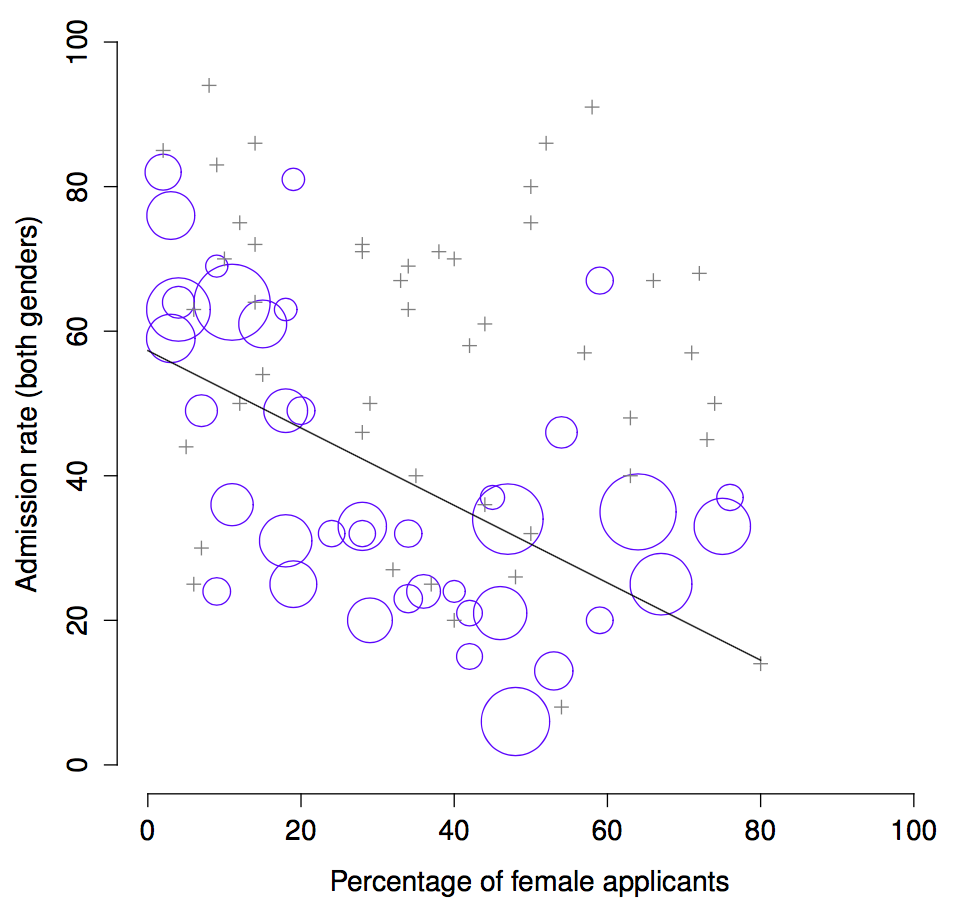
\includegraphics[width=0.75\textwidth,height=\textheight]{imgs/figures/1Simpson.png}

}

\caption{\label{fig-simpson}The Berkeley 1973 college admissions data.
This figure plots the admission rate for the 85 departments that had at
least one female applicant, as a function of the percentage of
applicants that were female. The plot is a redrawing of Figure 1 from
Bickel et al.~(1975). Circles plot departments with more than 40
applicants; the area of the circle is proportional to the total number
of applicants. The crosses plot department with fewer than 40
applicants.}

\end{figure}

Before leaving this topic entirely, I want to point out something else
really critical that is often overlooked in a research methods class.
Statistics only solves \emph{part} of the problem. Remember that we
started all this with the concern that Berkeley's admissions processes
might be unfairly biased against female applicants. When we looked at
the ``aggregated'' data, it did seem like the university was
discriminating against women, but when we ``disaggregate'' and looked at
the individual behavior of all the departments, it turned out that the
actual departments were, if anything, slightly biased in favor of women.
The gender bias in total admissions was caused by the fact that women
tended to self-select for harder departments. From a legal perspective,
that would probably put the university in the clear. Postgraduate
admissions are determined at the level of the individual department (and
there are good reasons to do that), and at the level of individual
departments, the decisions are more or less unbiased (the weak bias in
favor of females at that level is small, and not consistent across
departments). Since the university can't dictate which departments
people choose to apply to, and the decision making takes place at the
level of the department it can hardly be held accountable for any biases
that those choices produce.

That was the basis for my somewhat glib remarks earlier, but that's not
exactly the whole story, is it? After all, if we're interested in this
from a more sociological and psychological perspective, we might want to
ask \emph{why} there are such strong gender differences in applications.
Why do males tend to apply to engineering more often than females, and
why is this reversed for the English department? And why is it it the
case that the departments that tend to have a female-application bias
tend to have lower overall admission rates than those departments that
have a male-application bias? Might this not still reflect a gender
bias, even though every single department is itself unbiased? It might.
Suppose, hypothetically, that males preferred to apply to ``hard
sciences'' and females prefer ``humanities''. And suppose further that
the reason for why the humanities departments have low admission rates
is because the government doesn't want to fund the humanities (spots in
Ph.D.~programs, for instance, are often tied to government funded
research projects). Does that constitute a gender bias? Or just an
unenlightened view of the value of the humanities? What if someone at a
high level in the government cut the humanities funds because they felt
that the humanities are ``useless chick stuff''. That seems pretty
\emph{blatantly} gender biased. None of this falls within the purview of
statistics, but it matters to the research project. If you're interested
in the overall structural effects of subtle gender biases, then you
probably want to look at \emph{both} the aggregated and disaggregated
data. If you're interested in the decision making process at Berkeley
itself then you're probably only interested in the disaggregated data.

In short there are a lot of critical questions that you can't answer
with statistics, but the answers to those questions will have a huge
impact on how you analyse and interpret data. And this is the reason why
you should always think of statistics as a \emph{tool} to help you learn
about your data, no more and no less. It's a powerful tool to that end,
but there's no substitute for careful thought.

\hypertarget{statistics-in-environmental-science-why-all-the-numbers}{%
\section{Statistics in Environmental Science: Why All the
Numbers?}\label{statistics-in-environmental-science-why-all-the-numbers}}

You may wonder why your environmental science class is suddenly filled
with graphs, equations, and statistical terms. Why does environmental
science have so much statistics? Let me break it down for you!

\textbf{Why Does Environmental Science Need Statistics?}

It's a bit of a complex story, but let's face it: nature is complex too!
Unlike physics, where you might be studying straightforward things like
electrons, in environmental science, we're dealing with living
ecosystems, unpredictable weather, and human behavior.

Think of nature as a giant puzzle with pieces constantly changing shape.
We use statistics to piece it together. We're not dealing with simple
objects; we're dealing with the flow of rivers, the growth of forests,
and the migration of animals. It's a whole different ballgame.

In a sense, environmental scientists have to be part detective, part
mathematician. We need to understand statistics because we're solving
harder problems than some other fields. We're trying to make sense of
the messy, beautiful, and intricate web of life.

\textbf{Can't Someone Else Handle the Statistics?}

Sure, you could ask someone else to do the math, but here's the catch:
understanding statistics is crucial for understanding environmental
problems and solutions.

\begin{enumerate}
\def\labelenumi{\arabic{enumi}.}
\item
  \textbf{The Design Connection:} Want to research how pollution affects
  fish? You'll need to understand the statistics behind your study.
  Statistics and research design are like two sides of the same coin.
\item
  \textbf{Understanding the Science:} Want to read up on climate change?
  You'll find a lot of statistics in those papers. To truly get what's
  going on, you need to know what those numbers are saying.
\item
  \textbf{The Money Matter:} Hiring a statistician for every project?
  That'll cost you. Being self-sufficient in statistics means you can
  tackle more projects with fewer resources.
\end{enumerate}

\textbf{But What if I Don't Care About Jobs, Research, or Conservation?
Why Do I Need Statistics?}

Well, first of all, you've got me curious! But even if you're just an
everyday citizen, statistics matter. You're surrounded by data, whether
it's weather forecasts, pollution reports, or wildlife trends.

Knowing a bit about statistics is like having a decoder ring for the
modern world. It helps you understand the news, make informed decisions,
and even argue a point more convincingly.

So yes, statistics might feel like a strange guest in your environmental
science class. But trust me, it's a guest you want to get to know.
Because understanding statistics isn't just about crunching numbers;
it's about understanding our world and how we can make it better.

\hypertarget{statistics-in-everyday-life}{%
\section{Statistics in everyday
life}\label{statistics-in-everyday-life}}

\begin{quote}
\emph{``We are drowning in information,\\
but we are starved for knowledge''}\\

-- Various authors, original probably John Naisbitt
\end{quote}

When I started writing up my lecture notes I took the 20 most recent
news articles posted to the ABC news website. Of those 20 articles, it
turned out that 8 of them involved a discussion of something that I
would call a statistical topic; 6 of those made a mistake. The most
common error, if you're curious, was failing to report baseline data
(e.g., the article mentions that 5\% of people in situation X have some
characteristic Y, but doesn't say how common the characteristic is for
everyone else!) The point I'm trying to make here isn't that journalists
are bad at statistics (though they almost always are), it's that a basic
knowledge of statistics is very helpful for trying to figure out when
someone else is either making a mistake or even lying to you. Perhaps,
one of the biggest things that a knowledge of statistics does to you is
cause you to get angry at the newspaper or the internet on a far more
frequent basis :).

\hypertarget{theres-more-to-research-methods-than-statistics}{%
\section{There's more to research methods than
statistics}\label{theres-more-to-research-methods-than-statistics}}

So far, most of what I've talked about is statistics, and so you'd be
forgiven for thinking that statistics is all I care about in life. To be
fair, you wouldn't be far wrong, but research methodology is a broader
concept than statistics. So most research methods courses will cover a
lot of topics that relate much more to the pragmatics of research
design, and in particular the issues that you encounter when trying to
do research with humans. However, about 99\% of student \emph{fears}
relate to the statistics part of the course, so I've focused on the
stats in this discussion, and hopefully I've convinced you that
statistics matters, and more importantly, that it's not to be feared.
That being said, it's pretty typical for introductory research methods
classes to be very stats-heavy. This is not (usually) because the
lecturers are evil people. Quite the contrary, in fact. Introductory
classes focus a lot on the statistics because you almost always find
yourself needing statistics before you need the other research methods
training. Why? Because almost all of your assignments in other classes
will rely on statistical training, to a much greater extent than they
rely on other methodological tools. It's not common for undergraduate
assignments to require you to design your own study from the ground up
(in which case you would need to know a lot about research design), but
it \emph{is} common for assignments to ask you to analyse and interpret
data that were collected in a study that someone else designed (in which
case you need statistics). In that sense, from the perspective of
allowing you to do well in all your other classes, the statistics is
more urgent.

But note that ``urgent'' is different from ``important'' -- they both
matter. I really do want to stress that research design is just as
important as data analysis, and this book does spend a fair amount of
time on it. However, while statistics has a kind of universality, and
provides a set of core tools that are useful for most types of
psychological research, the research methods side isn't quite so
universal. There are some general principles that everyone should think
about, but a lot of research design is very idiosyncratic, and is
specific to the area of research that you want to engage in. To the
extent that it's the details that matter, those details don't usually
show up in an introductory stats and research methods class.

\hypertarget{a-brief-introduction-to-research-design}{%
\section{A brief introduction to research
design}\label{a-brief-introduction-to-research-design}}

In this chapter, we're going to start thinking about the basic ideas
that go into designing a study, collecting data, checking whether your
data collection works, and so on. It won't give you enough information
to allow you to design studies of your own, but it will give you a lot
of the basic tools that you need to assess the studies done by other
people. However, since the focus of this book is much more on data
analysis than on data collection, I'm only giving a very brief overview.
Note that this chapter is ``special'' in two ways. Firstly, it's much
more psychology-specific than the later chapters. Secondly, it focuses
much more heavily on the scientific problem of research methodology, and
much less on the statistical problem of data analysis. Nevertheless, the
two problems are related to one another, so it's traditional for stats
textbooks to discuss the problem in a little detail. This chapter relies
heavily on Campbell and Stanley (1963) for the discussion of study
design, and Stevens (1946) for the discussion of scales of measurement.
Later versions will attempt to be more precise in the citations.

\hypertarget{introduction-to-measurements}{%
\section{Introduction to
measurements}\label{introduction-to-measurements}}

The first thing to understand is data collection can be thought of as a
kind of \textbf{measurement}. That is, what we're trying to do here is
measure something about human behavior or the human mind. What do I mean
by ``measurement''?

\hypertarget{some-thoughts-about-measurements}{%
\subsection{Some thoughts about
measurements}\label{some-thoughts-about-measurements}}

Measurement itself is a subtle concept, but basically it comes down to
finding some way of assigning numbers, or labels, or some other kind of
well-defined descriptions to ``stuff''. So, any of the following would
count as a measurement:

\begin{itemize}
\item
  My \textbf{age} is \emph{33 years}.
\item
  I \emph{do not} \textbf{like anchovies}.
\item
  My \textbf{chromosomal gender} is \emph{male}.
\item
  My \textbf{self-identified gender} is \emph{male}.
\end{itemize}

In the short list above, the \textbf{bolded part} is ``the thing to be
measured'', and the \emph{italicized part} is ``the measurement
itself''. In fact, we can expand on this a little bit, by thinking about
the set of possible measurements that could have arisen in each case:

\begin{itemize}
\item
  My \textbf{age} (in years) could have been \emph{0, 1, 2, 3 \ldots{}},
  etc. The upper bound on what my age could possibly be is a bit fuzzy,
  but in practice you'd be safe in saying that the largest possible age
  is \emph{150}, since no human has ever lived that long.
\item
  When asked if I \textbf{like anchovies}, I might have said that
  \emph{I do}, or \emph{I do not}, or \emph{I have no opinion}, or
  \emph{I sometimes do}.
\item
  My \textbf{chromosomal gender} is almost certainly going to be
  \emph{male (XY)} or \emph{female (XX)}, but there are a few other
  possibilities. I could also have \emph{Klinfelter's syndrome (XXY)},
  which is more similar to male than to female. And I imagine there are
  other possibilities too.
\item
  My \textbf{self-identified gender} is also likely to be \emph{male} or
  \emph{female}, but it doesn't have to agree with my chromosomal
  gender. I may also choose to identify with \emph{neither}, or to
  explicitly call myself \emph{transgender}.
\end{itemize}

As you can see, for some things (like age) it seems fairly obvious what
the set of possible measurements should be, whereas for other things it
gets a bit tricky. But I want to point out that even in the case of
someone's age, it's much more subtle than this. For instance, in the
example above, I assumed that it was okay to measure age in years. But
if you're a developmental psychologist, that's way too crude, and so you
often measure age in \emph{years and months} (if a child is 2 years and
11 months, this is usually written as ``2;11''). If you're interested in
newborns, you might want to measure age in \emph{days since birth},
maybe even \emph{hours since birth}. In other words, the way in which
you specify the allowable measurement values is important.

Looking at this a bit more closely, you might also realize that the
concept of ``age'' isn't actually all that precise. In general, when we
say ``age'' we implicitly mean ``the length of time since birth''. But
that's not always the right way to do it. Suppose you're interested in
how newborn babies control their eye movements. If you're interested in
kids that young, you might also start to worry that ``birth'' is not the
only meaningful point in time to care about. If Baby Alice is born 3
weeks premature and Baby Bianca is born 1 week late, would it really
make sense to say that they are the ``same age'' if we encountered them
``2 hours after birth''? In one sense, yes: by social convention, we use
birth as our reference point for talking about age in everyday life,
since it defines the amount of time the person has been operating as an
independent entity in the world, but from a scientific perspective
that's not the only thing we care about. When we think about the biology
of human beings, it's often useful to think of ourselves as organisms
that have been growing and maturing since conception, and from that
perspective Alice and Bianca aren't the same age at all. So you might
want to define the concept of ``age'' in two different ways: the length
of time since conception, and the length of time since birth. When
dealing with adults, it won't make much difference, but when dealing
with newborns it might.

Moving beyond these issues, there's the question of methodology. What
specific ``measurement method'' are you going to use to find out
someone's age? As before, there are lots of different possibilities:

\begin{itemize}
\item
  You could just ask people ``how old are you?'' The method of
  self-report is fast, cheap and easy, but it only works with people old
  enough to understand the question, and some people lie about their
  age.
\item
  You could ask an authority (e.g., a parent) ``how old is your child?''
  This method is fast, and when dealing with kids it's not all that hard
  since the parent is almost always around. It doesn't work as well if
  you want to know ``age since conception'', since a lot of parents
  can't say for sure when conception took place. For that, you might
  need a different authority (e.g., an obstetrician).
\item
  You could look up official records, like birth certificates. This is
  time consuming and annoying, but it has its uses (e.g., if the person
  is now dead).
\end{itemize}

\hypertarget{operationalization-defining-your-measurement}{%
\subsection{Operationalization: defining your
measurement}\label{operationalization-defining-your-measurement}}

All of the ideas discussed in the previous section all relate to the
concept of \textbf{operationalization}. To be a bit more precise about
the idea, operationalization is the process by which we take a
meaningful but somewhat vague concept, and turn it into a precise
measurement. The process of operationalization can involve several
different things:

\begin{itemize}
\item
  Being precise about what you are trying to measure: For instance, does
  ``age'' mean ``time since birth'' or ``time since conception'' in the
  context of your research?
\item
  Determining what method you will use to measure it: Will you use
  self-report to measure age, ask a parent, or look up an official
  record? If you're using self-report, how will you phrase the question?
\item
  Defining the set of the allowable values that the measurement can
  take: Note that these values don't always have to be numerical, though
  they often are. When measuring age, the values are numerical, but we
  still need to think carefully about what numbers are allowed. Do we
  want age in years, years and months, days, hours? Etc. For other types
  of measurements (e.g., gender), the values aren't numerical. But, just
  as before, we need to think about what values are allowed. If we're
  asking people to self-report their gender, what options to we allow
  them to choose between? Is it enough to allow only ``male'' or
  ``female''? Do you need an ``other'' option? Or should we not give
  people any specific options, and let them answer in their own words?
  And if you open up the set of possible values to include all verbal
  response, how will you interpret their answers?
\end{itemize}

Operationalization is a tricky business, and there's no ``one, true
way'' to do it. The way in which you choose to operationalize the
informal concept of ``age'' or ``gender'' into a formal measurement
depends on what you need to use the measurement for. Often you'll find
that the community of scientists who work in your area have some fairly
well-established ideas for how to go about it. In other words,
operationalization needs to be thought through on a case by case basis.
Nevertheless, while there a lot of issues that are specific to each
individual research project, there are some aspects to it that are
pretty general.

Before moving on, I want to take a moment to clear up our terminology,
and in the process introduce one more term. Here are four different
things that are closely related to each other:

\begin{itemize}
\item
  \textbf{A theoretical construct}. This is the thing that you're trying
  to take a measurement of, like ``age'', ``gender'' or an ``opinion''.
  A theoretical construct can't be directly observed, and often they're
  actually a bit vague.
\item
  \textbf{A measure}. The measure refers to the method or the tool that
  you use to make your observations. A question in a survey, a
  behavioral observation or a brain scan could all count as a measure.
\item
  \textbf{An operationalization}. The term ``operationalization'' refers
  to the logical connection between the measure and the theoretical
  construct, or to the process by which we try to derive a measure from
  a theoretical construct.
\item
  \textbf{A variable}. Finally, a new term. A variable is what we end up
  with when we apply our measure to something in the world. That is,
  variables are the actual ``data'' that we end up with in our data
  sets.
\end{itemize}

In practice, even scientists tend to blur the distinction between these
things, but it's very helpful to try to understand the differences.

\hypertarget{scales-of-measurement}{%
\section{Scales of measurement}\label{scales-of-measurement}}

As the previous section indicates, the outcome of a psychological
measurement is called a variable. But not all variables are of the same
qualitative type, and it's very useful to understand what types there
are. A very useful concept for distinguishing between different types of
variables is what's known as \textbf{scales of measurement}.

\hypertarget{nominal-scale}{%
\subsection{Nominal scale}\label{nominal-scale}}

A \textbf{nominal scale} variable (also referred to as a
\textbf{categorical} variable) is one in which there is no particular
relationship between the different possibilities: for these kinds of
variables it doesn't make any sense to say that one of them is ``bigger'
or ``better'' than any other one, and it absolutely doesn't make any
sense to average them. The classic example for this is ``eye color''.
Eyes can be blue, green and brown, among other possibilities, but none
of them is any ``better'' than any other one. As a result, it would feel
really weird to talk about an ``average eye color''. Similarly, gender
is nominal too: male isn't better or worse than female, neither does it
make sense to try to talk about an ``average gender''. In short, nominal
scale variables are those for which the only thing you can say about the
different possibilities is that they are different. That's it.

Let's take a slightly closer look at this. Suppose I was doing research
on how people commute to and from work. One variable I would have to
measure would be what kind of transportation people use to get to work.
This ``transport type'' variable could have quite a few possible values,
including: ``train'', ``bus'', ``car'', ``bicycle'', etc. For now, let's
suppose that these four are the only possibilities, and suppose that
when I ask 100 people how they got to work today, and I get this:

\begin{longtable}[]{@{}lc@{}}
\toprule\noalign{}
Transportation & Number of people \\
\midrule\noalign{}
\endhead
\bottomrule\noalign{}
\endlastfoot
(1) Train & 12 \\
(2) Bus & 30 \\
(3) Car & 48 \\
(4) Bicycle & 10 \\
\end{longtable}

So, what's the average transportation type? Obviously, the answer here
is that there isn't one. It's a silly question to ask. You can say that
travel by car is the most popular method, and travel by train is the
least popular method, but that's about all. Similarly, notice that the
order in which I list the options isn't very interesting. I could have
chosen to display the data like this and nothing really changes.

\begin{longtable}[]{@{}lc@{}}
\toprule\noalign{}
Transportation & Number of people \\
\midrule\noalign{}
\endhead
\bottomrule\noalign{}
\endlastfoot
(3) Car & 48 \\
(1) Train & 12 \\
(4) Bicycle & 10 \\
(2) Bus & 30 \\
\end{longtable}

\hypertarget{ordinal-scale}{%
\subsection{Ordinal scale}\label{ordinal-scale}}

\textbf{Ordinal scale} variables have a bit more structure than nominal
scale variables, but not by a lot. An ordinal scale variable is one in
which there is a natural, meaningful way to order the different
possibilities, but you can't do anything else. The usual example given
of an ordinal variable is ``finishing position in a race''. You
\emph{can} say that the person who finished first was faster than the
person who finished second, but you \emph{don't} know how much faster.
As a consequence we know that 1st \(>\) 2nd, and we know that 2nd \(>\)
3rd, but the difference between 1st and 2nd might be much larger than
the difference between 2nd and 3rd.

Here's an more psychologically interesting example. Suppose I'm
interested in people's attitudes to climate change, and I ask them to
pick one of these four statements that most closely matches their
beliefs:

\begin{quote}
\begin{enumerate}
\def\labelenumi{(\arabic{enumi})}
\tightlist
\item
  Temperatures are rising, because of human activity\\
\item
  Temperatures are rising, but we don't know why\\
\item
  Temperatures are rising, but not because of humans\\
\item
  Temperatures are not rising
\end{enumerate}
\end{quote}

Notice that these four statements actually do have a natural ordering,
in terms of ``the extent to which they agree with the current science''.
Statement 1 is a close match, statement 2 is a reasonable match,
statement 3 isn't a very good match, and statement 4 is in strong
opposition to the science. So, in terms of the thing I'm interested in
(the extent to which people endorse the science), I can order the items
as \(1 > 2 > 3 > 4\). Since this ordering exists, it would be very weird
to list the options like this\ldots{}

\begin{quote}
\begin{enumerate}
\def\labelenumi{(\arabic{enumi})}
\setcounter{enumi}{2}
\tightlist
\item
  Temperatures are rising, but not because of humans\\
\item
  Temperatures are rising, because of human activity\\
\item
  Temperatures are not rising\\
\item
  Temperatures are rising, but we don't know why
\end{enumerate}
\end{quote}

\ldots because it seems to violate the natural ``structure'' to the
question.

So, let's suppose I asked 100 people these questions, and got the
following answers:

\begin{longtable}[]{@{}lc@{}}
\toprule\noalign{}
& Number \\
\midrule\noalign{}
\endhead
\bottomrule\noalign{}
\endlastfoot
(1) Temperatures are rising, because of human activity & 51 \\
(2) Temperatures are rising, but we don't know why & 20 \\
(3) Temperatures are rising, but not because of humans & 10 \\
(4) Temperatures are not rising & 19 \\
\end{longtable}

When analyzing these data, it seems quite reasonable to try to group
(1), (2) and (3) together, and say that 81 of 100 people were willing to
\emph{at least partially} endorse the science. And it's \emph{also}
quite reasonable to group (2), (3) and (4) together and say that 49 of
100 people registered \emph{at least some disagreement} with the
dominant scientific view. However, it would be entirely bizarre to try
to group (1), (2) and (4) together and say that 90 of 100 people
said\ldots what? There's nothing sensible that allows you to group those
responses together at all.

That said, notice that while we \emph{can} use the natural ordering of
these items to construct sensible groupings, what we \emph{can't} do is
average them. For instance, in my simple example here, the ``average''
response to the question is 1.97. If you can tell me what that means,
I'd love to know. Because that sounds like gibberish to me!

\hypertarget{interval-scale}{%
\subsection{Interval scale}\label{interval-scale}}

In contrast to nominal and ordinal scale variables, \textbf{interval
scale} and ratio scale variables are variables for which the numerical
value is genuinely meaningful. In the case of interval scale variables,
the \emph{differences} between the numbers are interpretable, but the
variable doesn't have a ``natural'' zero value. A good example of an
interval scale variable is measuring temperature in degrees Celsius. For
instance, if it was 15\(^\circ\) yesterday and 18\(^\circ\) today, then
the 3\(^\circ\) difference between the two is genuinely meaningful.
Moreover, that 3\(^\circ\) difference is \emph{exactly the same} as the
3\(^\circ\) difference between \(7^\circ\) and \(10^\circ\). In short,
addition and subtraction are meaningful for interval scale variables.

However, notice that the \(0^\circ\) does not mean ``no temperature at
all'': it actually means ``the temperature at which water freezes'',
which is pretty arbitrary. As a consequence, it becomes pointless to try
to multiply and divide temperatures. It is wrong to say that
\(20^\circ\) is \emph{twice as hot} as \(10^\circ\), just as it is weird
and meaningless to try to claim that \(20^\circ\) is negative two times
as hot as \(-10^\circ\).

Again, lets look at a more psychological example. Suppose I'm interested
in looking at how the attitudes of first-year university students have
changed over time. Obviously, I'm going to want to record the year in
which each student started. This is an interval scale variable. A
student who started in 2003 did arrive 5 years before a student who
started in 2008. However, it would be completely insane for me to divide
2008 by 2003 and say that the second student started ``1.0024 times
later'' than the first one. That doesn't make any sense at all.

\hypertarget{ratio-scale}{%
\subsection{Ratio scale}\label{ratio-scale}}

The fourth and final type of variable to consider is a \textbf{ratio
scale} variable, in which zero really means zero, and it's okay to
multiply and divide. A good psychological example of a ratio scale
variable is response time (RT). In a lot of tasks it's very common to
record the amount of time somebody takes to solve a problem or answer a
question, because it's an indicator of how difficult the task is.
Suppose that Alan takes 2.3 seconds to respond to a question, whereas
Ben takes 3.1 seconds. As with an interval scale variable, addition and
subtraction are both meaningful here. Ben really did take
\(3.1 - 2.3 = 0.8\) seconds longer than Alan did. However, notice that
multiplication and division also make sense here too: Ben took
\(3.1 / 2.3 = 1.35\) times as long as Alan did to answer the question.
And the reason why you can do this is that, for a ratio scale variable
such as RT, ``zero seconds'' really does mean ``no time at all''.

\hypertarget{continuous-versus-discrete-variables}{%
\subsection{Continuous versus discrete
variables}\label{continuous-versus-discrete-variables}}

There's a second kind of distinction that you need to be aware of,
regarding what types of variables you can run into. This is the
distinction between continuous variables and discrete variables. The
difference between these is as follows:

\begin{itemize}
\item
  A \textbf{continuous variable} is one in which, for any two values
  that you can think of, it's always logically possible to have another
  value in between.
\item
  A \textbf{discrete variable} is, in effect, a variable that isn't
  continuous. For a discrete variable, it's sometimes the case that
  there's nothing in the middle.
\end{itemize}

These definitions probably seem a bit abstract, but they're pretty
simple once you see some examples. For instance, response time is
continuous. If Alan takes 3.1 seconds and Ben takes 2.3 seconds to
respond to a question, then it's possible for Cameron's response time to
lie in between, by taking 3.0 seconds. And of course it would also be
possible for David to take 3.031 seconds to respond, meaning that his RT
would lie in between Cameron's and Alan's. And while in practice it
might be impossible to measure RT that precisely, it's certainly
possible in principle. Because we can always find a new value for RT in
between any two other ones, we say that RT is continuous.

Discrete variables occur when this rule is violated. For example,
nominal scale variables are always discrete: there isn't a type of
transportation that falls ``in between'' trains and bicycles, not in the
strict mathematical way that 2.3 falls in between 2 and 3. So
transportation type is discrete. Similarly, ordinal scale variables are
always discrete: although ``2nd place'' does fall between ``1st place''
and ``3rd place'', there's nothing that can logically fall in between
``1st place'' and ``2nd place''. Interval scale and ratio scale
variables can go either way. As we saw above, response time (a ratio
scale variable) is continuous. Temperature in degrees Celsius (an
interval scale variable) is also continuous. However, the year you went
to school (an interval scale variable) is discrete. There's no year in
between 2002 and 2003. The number of questions you get right on a
true-or-false test (a ratio scale variable) is also discrete: since a
true-or-false question doesn't allow you to be ``partially correct'',
there's nothing in between 5/10 and 6/10. The table summarizes the
relationship between the scales of measurement and the
discrete/continuity distinction. Cells with a tick mark correspond to
things that are possible. I'm trying to hammer this point home, because
(a) some textbooks get this wrong, and (b) people very often say things
like ``discrete variable'' when they mean ``nominal scale variable''.
It's very unfortunate.

\begin{longtable}[]{@{}lcc@{}}
\caption{The relationship between the scales of measurement and the
discrete/continuity distinction. Cells with an x correspond to things
that are possible.}\tabularnewline
\toprule\noalign{}
& continuous & discrete \\
\midrule\noalign{}
\endfirsthead
\toprule\noalign{}
& continuous & discrete \\
\midrule\noalign{}
\endhead
\bottomrule\noalign{}
\endlastfoot
nominal & & x \\
ordinal & & x \\
interval & x & x \\
ratio & x & x \\
\end{longtable}

\hypertarget{some-complexities}{%
\subsection{Some complexities}\label{some-complexities}}

Okay, I know you're going to be shocked to hear this, but \ldots the
real world is much messier than this little classification scheme
suggests. Very few variables in real life actually fall into these nice
neat categories, so you need to be kind of careful not to treat the
scales of measurement as if they were hard and fast rules. It doesn't
work like that: they're guidelines, intended to help you think about the
situations in which you should treat different variables differently.
Nothing more.

So let's take a classic example, maybe \emph{the} classic example, of a
psychological measurement tool: the \textbf{Likert scale}. The humble
Likert scale is the bread and butter tool of all survey design. You
yourself have filled out hundreds, maybe thousands of them, and odds are
you've even used one yourself. Suppose we have a survey question that
looks like this:

\begin{quote}
Which of the following best describes your opinion of the statement that
``all pirates are freaking awesome'' \ldots{}
\end{quote}

and then the options presented to the participant are these:

\begin{quote}
(1) Strongly disagree\\
(2) Disagree\\
(3) Neither agree nor disagree\\
(4) Agree\\
(5) Strongly agree
\end{quote}

This set of items is an example of a 5-point Likert scale: people are
asked to choose among one of several (in this case 5) clearly ordered
possibilities, generally with a verbal descriptor given in each case.
However, it's not necessary that all items be explicitly described. This
is a perfectly good example of a 5-point Likert scale too:

\begin{quote}
(1) Strongly disagree\\
(2)\\
(3)\\
(4)\\
(5) Strongly agree
\end{quote}

Likert scales are very handy, if somewhat limited, tools. The question
is, what kind of variable are they? They're obviously discrete, since
you can't give a response of 2.5. They're obviously not nominal scale,
since the items are ordered; and they're not ratio scale either, since
there's no natural zero.

But are they ordinal scale or interval scale? One argument says that we
can't really prove that the difference between ``strongly agree'' and
``agree'' is of the same size as the difference between ``agree'' and
``neither agree nor disagree''. In fact, in everyday life it's pretty
obvious that they're not the same at all. So this suggests that we ought
to treat Likert scales as ordinal variables. On the other hand, in
practice most participants do seem to take the whole ``on a scale from 1
to 5'' part fairly seriously, and they tend to act as if the differences
between the five response options were fairly similar to one another. As
a consequence, a lot of researchers treat Likert scale data as if it
were interval scale. It's not interval scale, but in practice it's close
enough that we usually think of it as being \textbf{quasi-interval
scale}.

\hypertarget{assessing-the-reliability-of-a-measurement}{%
\section{Assessing the reliability of a
measurement}\label{assessing-the-reliability-of-a-measurement}}

At this point we've thought a little bit about how to operationalize a
theoretical construct and thereby create a psychological measure; and
we've seen that by applying psychological measures we end up with
variables, which can come in many different types. At this point, we
should start discussing the obvious question: is the measurement any
good? We'll do this in terms of two related ideas: \emph{reliability}
and \emph{validity}. Put simply, the \textbf{reliability} of a measure
tells you how \emph{precisely} you are measuring something, whereas the
validity of a measure tells you how \emph{accurate} the measure is.

Reliability is actually a very simple concept: it refers to the
repeatability or consistency of your measurement. The measurement of my
weight by means of a ``bathroom scale'' is very reliable: if I step on
and off the scales over and over again, it'll keep giving me the same
answer. Measuring my intelligence by means of ``asking my mom'' is very
unreliable: some days she tells me I'm a bit thick, and other days she
tells me I'm a complete moron. Notice that this concept of reliability
is different to the question of whether the measurements are correct
(the correctness of a measurement relates to it's validity). If I'm
holding a sack of potatoes when I step on and off of the bathroom
scales, the measurement will still be reliable: it will always give me
the same answer. However, this highly reliable answer doesn't match up
to my true weight at all, therefore it's wrong. In technical terms, this
is a \emph{reliable but invalid} measurement. Similarly, while my mom's
estimate of my intelligence is a bit unreliable, she might be right.
Maybe I'm just not too bright, and so while her estimate of my
intelligence fluctuates pretty wildly from day to day, it's basically
right. So that would be an \emph{unreliable but valid} measure. Of
course, to some extent, notice that if my mum's estimates are too
unreliable, it's going to be very hard to figure out which one of her
many claims about my intelligence is actually the right one. To some
extent, then, a very unreliable measure tends to end up being invalid
for practical purposes; so much so that many people would say that
reliability is necessary (but not sufficient) to ensure validity.

Okay, now that we're clear on the distinction between reliability and
validity, let's have a think about the different ways in which we might
measure reliability:

\begin{itemize}
\item
  \textbf{Test-retest reliability}. This relates to consistency over
  time: if we repeat the measurement at a later date, do we get a the
  same answer?
\item
  \textbf{Inter-rater reliability}. This relates to consistency across
  people: if someone else repeats the measurement (e.g., someone else
  rates my intelligence) will they produce the same answer?
\item
  \textbf{Parallel forms reliability}. This relates to consistency
  across theoretically-equivalent measurements: if I use a different set
  of bathroom scales to measure my weight, does it give the same answer?
\item
  \textbf{Internal consistency reliability}. If a measurement is
  constructed from lots of different parts that perform similar
  functions (e.g., a personality questionnaire result is added up across
  several questions) do the individual parts tend to give similar
  answers.
\end{itemize}

Not all measurements need to possess all forms of reliability. For
instance, educational assessment can be thought of as a form of
measurement. One of the subjects that I teach, \emph{Inroduction to
Environmental Science}, has an assessment structure that has a
presentation component and an exam component (plus other things). The
exam component is \emph{intended} to measure something different from
the presentation component, so the assessment as a whole has low
internal consistency. However, within the exam there are several
questions that are intended to (approximately) measure the same things,
and those tend to produce similar outcomes; so the exam on its own has a
fairly high internal consistency. Which is as it should be. You should
only demand reliability in those situations where you want to be measure
the same thing!

\hypertarget{the-role-of-variables-predictors-and-outcomes}{%
\section{The role of variables: predictors and
outcomes}\label{the-role-of-variables-predictors-and-outcomes}}

Okay, I've got one last piece of terminology that I need to explain to
you before moving away from variables. Normally, when we do some
research we end up with lots of different variables. Then, when we
analyse our data we usually try to explain some of the variables in
terms of some of the other variables. It's important to keep the two
roles ``thing doing the explaining'' and ``thing being explained''
distinct. So let's be clear about this now. Firstly, we might as well
get used to the idea of using mathematical symbols to describe
variables, since it's going to happen over and over again. Let's denote
the ``to be explained'' variable \(Y\), and denote the variables ``doing
the explaining'' as \(X_1\), \(X_2\), etc.

Now, when we doing an analysis, we have different names for \(X\) and
\(Y\), since they play different roles in the analysis. The classical
names for these roles are \textbf{independent variable} (IV) and
\textbf{dependent variable} (DV). The IV is the variable that you use to
do the explaining (i.e., \(X\)) and the DV is the variable being
explained (i.e., \(Y\)). The logic behind these names goes like this: if
there really is a relationship between \(X\) and \(Y\) then we can say
that \(Y\) depends on \(X\), and if we have designed our study
``properly'' then \(X\) isn't dependent on anything else. However, I
personally find those names horrible: they're hard to remember and
they're highly misleading, because (a) the IV is never actually
``independent of everything else'' and (b) if there's no relationship,
then the DV doesn't actually depend on the IV. And in fact, because I'm
not the only person who thinks that IV and DV are just awful names,
there are a number of alternatives that I find more appealing.

For example, in an experiment the IV refers to the
\textbf{manipulation}, and the DV refers to the \textbf{measurement}.
So, we could use \textbf{manipulated variable} (independent variable)
and \textbf{measured variable} (dependent variable).

\begin{longtable}[]{@{}lll@{}}
\caption{The terminology used to distinguish between different roles
that a variable can play when analyzing a data set.}\tabularnewline
\toprule\noalign{}
role of the variable & classical name & modern name \\
\midrule\noalign{}
\endfirsthead
\toprule\noalign{}
role of the variable & classical name & modern name \\
\midrule\noalign{}
\endhead
\bottomrule\noalign{}
\endlastfoot
``to be explained'' & dependent variable (DV) & Measurement \\
``to do the explaining'' & independent variable (IV) & Manipulation \\
\end{longtable}

We could also use \textbf{predictors} and \textbf{outcomes}. The idea
here is that what you're trying to do is use \(X\) (the predictors) to
make guesses about \(Y\) (the outcomes). This is summarized in the
table:

\begin{longtable}[]{@{}lll@{}}
\caption{The terminology used to distinguish between different roles
that a variable can play when analyzing a data set.}\tabularnewline
\toprule\noalign{}
role of the variable & classical name & modern name \\
\midrule\noalign{}
\endfirsthead
\toprule\noalign{}
role of the variable & classical name & modern name \\
\midrule\noalign{}
\endhead
\bottomrule\noalign{}
\endlastfoot
``to be explained'' & dependent variable (DV) & outcome \\
``to do the explaining'' & independent variable (IV) & predictor \\
\end{longtable}

\hypertarget{experimental-and-non-experimental-research}{%
\section{Experimental and non-experimental
research}\label{experimental-and-non-experimental-research}}

One of the big distinctions that you should be aware of is the
distinction between ``experimental research'' and ``non-experimental
research''. When we make this distinction, what we're really talking
about is the degree of control that the researcher exercises over the
people and events in the study.

\hypertarget{experimental-research}{%
\subsection{Experimental research}\label{experimental-research}}

The key features of \textbf{experimental research} is that the
researcher controls all aspects of the study, especially what
participants experience during the study. In particular, the researcher
manipulates or varies something (IVs), and then allows the outcome
variable (DV) to vary naturally. The idea here is to deliberately vary
the something in the world (IVs) to see if it has any causal effects on
the outcomes. Moreover, in order to ensure that there's no chance that
something other than the manipulated variable is causing the outcomes,
everything else is kept constant or is in some other way ``balanced'' to
ensure that they have no effect on the results. In practice, it's almost
impossible to \emph{think} of everything else that might have an
influence on the outcome of an experiment, much less keep it constant.
The standard solution to this is \textbf{randomization}: that is, we
randomly assign people to different groups, and then give each group a
different treatment (i.e., assign them different values of the predictor
variables). We'll talk more about randomization later in this course,
but for now, it's enough to say that what randomization does is minimize
(but not eliminate) the chances that there are any systematic difference
between groups.

Let's consider a very simple, completely unrealistic and grossly
unethical example. Suppose you wanted to find out if smoking causes lung
cancer. One way to do this would be to find people who smoke and people
who don't smoke, and look to see if smokers have a higher rate of lung
cancer. This is \emph{not} a proper experiment, since the researcher
doesn't have a lot of control over who is and isn't a smoker. And this
really matters: for instance, it might be that people who choose to
smoke cigarettes also tend to have poor diets, or maybe they tend to
work in asbestos mines, or whatever. The point here is that the groups
(smokers and non-smokers) actually differ on lots of things, not
\emph{just} smoking. So it might be that the higher incidence of lung
cancer among smokers is caused by something else, not by smoking per se.
In technical terms, these other things (e.g.~diet) are called
``confounds'', and we'll talk about those in just a moment.

In the meantime, let's now consider what a proper experiment might look
like. Recall that our concern was that smokers and non-smokers might
differ in lots of ways. The solution, as long as you have no ethics, is
to \emph{control} who smokes and who doesn't. Specifically, if we
randomly divide participants into two groups, and force half of them to
become smokers, then it's very unlikely that the groups will differ in
any respect other than the fact that half of them smoke. That way, if
our smoking group gets cancer at a higher rate than the non-smoking
group, then we can feel pretty confident that (a) smoking does cause
cancer and (b) we're murderers.

\hypertarget{non-experimental-research}{%
\subsection{Non-experimental research}\label{non-experimental-research}}

\textbf{Non-experimental research} in environmental science often
encompasses studies in which researchers cannot exert full control over
variables as they might in a typical experimental setup. In
environmental science, this issue is particularly pronounced, as there
is no ``control planet'' to allow for perfect experimental conditions.
This unique challenge leads to a reliance on alternative approaches,
such as time series analysis, to understand complex environmental
phenomena.

One distinction worth making between two types of non-experimental
research is the difference between \textbf{quasi-experimental research}
and \textbf{case studies}. Much of the research in environmental science
fits into a quasi-experimental design. Here, researchers might wish to
study the effects of industrial pollution on a river system but cannot
directly control all the variables, such as the quantity or type of
pollutants being emitted by various industries. Instead, they must
observe existing conditions and make careful comparisons, possibly using
statistical tools to account for confounding variables.

\textbf{Time series analysis} becomes vital in this context, as many
environmental processes unfold over extended periods. For example,
tracking changes in global temperatures or sea level requires years of
consistent data collection. The complexity and variability inherent in
environmental systems make drawing definitive conclusions difficult, but
sophisticated statistical methods can help isolate specific effects.

Environmental science also frequently relies on detailed \textbf{case
studies}. These investigations focus on particular events or locations
to provide in-depth insights into environmental processes and their
impacts on ecosystems, human health, and societal structures. Case
studies might explore the aftermath of a natural disaster, the unique
ecology of a threatened habitat, or the social and economic consequences
of environmental policies.

Though they often lack the broad generalizability of more controlled
experimental research, case studies in environmental science offer
valuable opportunities to understand the complexity of real-world
situations. They can uncover nuances and subtleties that might be
overlooked in a broader experimental or quasi-experimental approach.

The absence of a control planet and the complexity of environmental
systems necessitates flexible and often non-traditional approaches to
scientific inquiry in environmental science. While these methods,
including quasi-experimental designs and case studies, may not offer the
same level of control as experimental designs, they are indispensable
tools in the field. By leveraging time series data, employing careful
statistical analysis, and embracing the rich insights offered by focused
case studies, researchers can continue to expand our understanding of
the biosphere and its interactions with human activities.

\hypertarget{assessing-the-validity-of-a-study}{%
\section{Assessing the validity of a
study}\label{assessing-the-validity-of-a-study}}

More than any other thing, a scientist wants their research to be
``valid''. The conceptual idea behind \textbf{validity} is very simple:
can you trust the results of your study? If not, the study is invalid.
However, while it's easy to state, in practice it's much harder to check
validity than it is to check reliability. And in all honesty, there's no
precise, clearly agreed upon notion of what validity actually is. In
fact, there's lots of different kinds of validity, each of which raises
it's own issues, and not all forms of validity are relevant to all
studies. I'm going to talk about five different types:

\begin{itemize}
\item
  Internal validity
\item
  External validity
\item
  Construct validity
\item
  Face validity
\item
  Ecological validity
\end{itemize}

To give you a quick guide as to what matters here\ldots(1) Internal and
external validity are the most important, since they tie directly to the
fundamental question of whether your study really works. (2) Construct
validity asks whether you're measuring what you think you are. (3) Face
validity isn't terribly important except insofar as you care about
``appearances''. (4) Ecological validity is a special case of face
validity that corresponds to a kind of appearance that you might care
about a lot.

\hypertarget{internal-validity}{%
\subsection{Internal validity}\label{internal-validity}}

\textbf{Internal validity} refers to the extent to which you are able
draw the correct conclusions about the causal relationships between
variables. It's called ``internal'' because it refers to the
relationships between things ``inside'' the study. Let's illustrate the
concept with a simple example. Suppose you're interested in finding out
whether a university education makes you write better. To do so, you get
a group of first year students, ask them to write a 1000 word essay, and
count the number of spelling and grammatical errors they make. Then you
find some third-year students, who obviously have had more of a
university education than the first-years, and repeat the exercise. And
let's suppose it turns out that the third-year students produce fewer
errors. And so you conclude that a university education improves writing
skills. Right? Except\ldots{} the big problem that you have with this
experiment is that the third-year students are older, and they've had
more experience with writing things. So it's hard to know for sure what
the causal relationship is: Do older people write better? Or people who
have had more writing experience? Or people who have had more education?
Which of the above is the true \emph{cause} of the superior performance
of the third-years? Age? Experience? Education? You can't tell. This is
an example of a failure of internal validity, because your study doesn't
properly tease apart the \emph{causal} relationships between the
different variables.

\hypertarget{external-validity}{%
\subsection{External validity}\label{external-validity}}

\textbf{External validity} relates to the \textbf{generalizability} of
your findings. That is, to what extent do you expect to see the same
pattern of results in ``real life'' as you saw in your study. To put it
a bit more precisely, any study that you do in psychology will involve a
fairly specific set of questions or tasks, will occur in a specific
environment, and will involve participants that are drawn from a
particular subgroup. So, if it turns out that the results don't actually
generalize to people and situations beyond the ones that you studied,
then what you've got is a lack of external validity.

The classic example of this issue is the fact that a very large
proportion of studies in psychology will use undergraduate psychology
students as the participants. Obviously, however, the researchers don't
care \emph{only} about psychology students; they care about people in
general. Given that, a study that uses only psych students as
participants always carries a risk of lacking external validity. That
is, if there's something ``special'' about psychology students that
makes them different to the general populace in some \emph{relevant}
respect, then we may start worrying about a lack of external validity.

That said, it is absolutely critical to realize that a study that uses
only psychology students does not necessarily have a problem with
external validity. I'll talk about this again later, but it's such a
common mistake that I'm going to mention it here. The external validity
is threatened by the choice of population if (a) the population from
which you sample your participants is very narrow (e.g., psych
students), and (b) the narrow population that you sampled from is
systematically different from the general population, \emph{in some
respect that is relevant to the psychological phenomenon that you intend
to study}. The italicized part is the bit that lots of people forget: it
is true that psychology undergraduates differ from the general
population in lots of ways, and so a study that uses only psych students
\emph{may} have problems with external validity. However, if those
differences aren't very relevant to the phenomenon that you're studying,
then there's nothing to worry about. To make this a bit more concrete,
here's two extreme examples:

\begin{itemize}
\item
  You want to measure ``attitudes of the general public towards
  psychotherapy'', but all of your participants are psychology students.
  This study would almost certainly have a problem with external
  validity.
\item
  You want to measure the effectiveness of a visual illusion, and your
  participants are all psychology students. This study is very unlikely
  to have a problem with external validity
\end{itemize}

Having just spent the last couple of paragraphs focusing on the choice
of participants (since that's the big issue that everyone tends to worry
most about), it's worth remembering that external validity is a broader
concept. The following are also examples of things that might pose a
threat to external validity, depending on what kind of study you're
doing:

\begin{itemize}
\item
  People might answer a ``psychology questionnaire'' in a manner that
  doesn't reflect what they would do in real life.
\item
  Your lab experiment on (say) ``human learning'' has a different
  structure to the learning problems people face in real life.
\end{itemize}

\hypertarget{construct-validity}{%
\subsection{Construct validity}\label{construct-validity}}

\textbf{Construct validity} is basically a question of whether you're
measuring what you want to be measuring. A measurement has good
construct validity if it is actually measuring the correct theoretical
construct, and bad construct validity if it doesn't. To give very simple
(if ridiculous) example, suppose I'm trying to investigate the rates
with which university students cheat on their exams. And the way I
attempt to measure it is by asking the cheating students to stand up in
the lecture theater so that I can count them. When I do this with a
class of 300 students, 0 people claim to be cheaters. So I therefore
conclude that the proportion of cheaters in my class is 0\%. Clearly
this is a bit ridiculous. But the point here is not that this is a very
deep methodological example, but rather to explain what construct
validity is. The problem with my measure is that while I'm \emph{trying}
to measure ``the proportion of people who cheat'' what I'm actually
measuring is ``the proportion of people stupid enough to own up to
cheating, or bloody minded enough to pretend that they do''. Obviously,
these aren't the same thing! So my study has gone wrong, because my
measurement has very poor construct validity.

\hypertarget{face-validity}{%
\subsection{Face validity}\label{face-validity}}

\textbf{Face validity} simply refers to whether or not a measure ``looks
like'' it's doing what it's supposed to, nothing more. If I design a
test of intelligence, and people look at it and they say ``no, that test
doesn't measure intelligence'', then the measure lacks face validity.
It's as simple as that. Obviously, face validity isn't very important
from a pure scientific perspective. After all, what we care about is
whether or not the measure \emph{actually} does what it's supposed to
do, not whether it \emph{looks like} it does what it's supposed to do.
As a consequence, we generally don't care very much about face validity.
That said, the concept of face validity serves three useful pragmatic
purposes:

\begin{itemize}
\item
  Sometimes, an experienced scientist will have a ``hunch'' that a
  particular measure won't work. While these sorts of hunches have no
  strict evidentiary value, it's often worth paying attention to them.
  Because often times people have knowledge that they can't quite
  verbalize, so there might be something to worry about even if you
  can't quite say why. In other words, when someone you trust criticizes
  the face validity of your study, it's worth taking the time to think
  more carefully about your design to see if you can think of reasons
  why it might go awry. Mind you, if you don't find any reason for
  concern, then you should probably not worry: after all, face validity
  really doesn't matter much.
\item
  Often (very often), completely uninformed people will also have a
  ``hunch'' that your research is crap. And they'll criticize it on the
  internet or something. On close inspection, you'll often notice that
  these criticisms are actually focused entirely on how the study
  ``looks'', but not on anything deeper. The concept of face validity is
  useful for gently explaining to people that they need to substantiate
  their arguments further.
\item
  Expanding on the last point, if the beliefs of untrained people are
  critical (e.g., this is often the case for applied research where you
  actually want to convince policy makers of something or other) then
  you \emph{have} to care about face validity. Simply because -- whether
  you like it or not -- a lot of people will use face validity as a
  proxy for real validity. If you want the government to change a law on
  scientific, psychological grounds, then it won't matter how good your
  studies ``really'' are. If they lack face validity, you'll find that
  politicians ignore you. Of course, it's somewhat unfair that policy
  often depends more on appearance than fact, but that's how things go.
\end{itemize}

\hypertarget{ecological-validity}{%
\subsection{Ecological validity}\label{ecological-validity}}

\textbf{Ecological validity} is a different notion of validity, which is
similar to external validity, but less important. The idea is that, in
order to be ecologically valid, the entire set up of the study should
closely approximate the real world scenario that is being investigated.
In a sense, ecological validity is a kind of face validity -- it relates
mostly to whether the study ``looks'' right, but with a bit more rigor
to it. To be ecologically valid, the study has to look right in a fairly
specific way. The idea behind it is the intuition that a study that is
ecologically valid is more likely to be externally valid. It's no
guarantee, of course. But the nice thing about ecological validity is
that it's much easier to check whether a study is ecologically valid
than it is to check whether a study is externally valid. An simple
example would be eyewitness identification studies. Most of these
studies tend to be done in a university setting, often with fairly
simple array of faces to look at rather than a line up. The length of
time between seeing the ``criminal'' and being asked to identify the
suspect in the ``line up'' is usually shorter. The ``crime'' isn't real,
so there's no chance that the witness being scared, and there's no
police officers present, so there's not as much chance of feeling
pressured. These things all mean that the study \emph{definitely} lacks
ecological validity. They might (but might not) mean that it also lacks
external validity.

\hypertarget{confounds-artifacts-and-other-threats-to-validity}{%
\section{Confounds, artifacts and other threats to
validity}\label{confounds-artifacts-and-other-threats-to-validity}}

If we look at the issue of validity in the most general fashion, the two
biggest worries that we have are \emph{confounds} and \emph{artifact}.
These two terms are defined in the following way:

\begin{itemize}
\item
  \textbf{Confound}: A confound is an additional, often unmeasured
  variable that turns out to be related to both the predictors and the
  outcomes. The existence of confounds threatens the internal validity
  of the study because you can't tell whether the predictor causes the
  outcome, or if the confounding variable causes it, etc.
\item
  \textbf{Artifact}: A result is said to be ``artifactual'' if it only
  holds in the special situation that you happened to test in your
  study. The possibility that your result is an artifact describes a
  threat to your external validity, because it raises the possibility
  that you can't generalize your results to the actual population that
  you care about.
\end{itemize}

As a general rule confounds are a bigger concern for non-experimental
studies, precisely because they're not proper experiments: by
definition, you're leaving lots of things uncontrolled, so there's a lot
of scope for confounds working their way into your study. Experimental
research tends to be much less vulnerable to confounds: the more control
you have over what happens during the study, the more you can prevent
confounds from appearing.

However, there's always swings and roundabouts, and when we start
thinking about artifacts rather than confounds, the shoe is very firmly
on the other foot. For the most part, artifactual results tend to be a
concern for experimental studies than for non-experimental studies. To
see this, it helps to realize that the reason that a lot of studies are
non-experimental is precisely because what the researcher is trying to
do is examine human behavior in a more naturalistic context. By working
in a more real-world context, you lose experimental control (making
yourself vulnerable to confounds) but because you tend to be studying
human psychology ``in the wild'' you reduce the chances of getting an
artifactual result. Or, to put it another way, when you take psychology
out of the wild and bring it into the lab (which we usually have to do
to gain our experimental control), you always run the risk of
accidentally studying something different than you wanted to study:
which is more or less the definition of an artifact.

Be warned though: the above is a rough guide only. It's absolutely
possible to have confounds in an experiment, and to get artifactual
results with non-experimental studies. This can happen for all sorts of
reasons, not least of which is researcher error. In practice, it's
really hard to think everything through ahead of time, and even very
good researchers make mistakes. But other times it's unavoidable, simply
because the researcher has ethics (e.g., see ``differential
attrition'').

Okay. There's a sense in which almost any threat to validity can be
characterized as a confound or an artifact: they're pretty vague
concepts. So let's have a look at some of the most common
examples\ldots{}

\hypertarget{history-effects}{%
\subsection{History effects}\label{history-effects}}

\textbf{History effects} refer to the possibility that specific events
may occur during the study itself that might influence the outcomes. For
instance, something might happen in between a pre-test and a post-test.
Or, in between testing participant 23 and participant 24. Alternatively,
it might be that you're looking at an older study, which was perfectly
valid for its time, but the world has changed enough since then that the
conclusions are no longer trustworthy. Examples of things that would
count as history effects:

\begin{itemize}
\item
  You're interested in how people think about risk and uncertainty. You
  started your data collection in December 2010. But finding
  participants and collecting data takes time, so you're still finding
  new people in February 2011. Unfortunately for you (and even more
  unfortunately for others), the Queensland floods occurred in January
  2011, causing billions of dollars of damage and killing many people.
  Not surprisingly, the people tested in February 2011 express quite
  different beliefs about handling risk than the people tested in
  December 2010. Which (if any) of these reflects the ``true'' beliefs
  of participants? I think the answer is probably both: the Queensland
  floods genuinely changed the beliefs of the Australian public, though
  possibly only temporarily. The key thing here is that the ``history''
  of the people tested in February is quite different to people tested
  in December.
\item
  You're testing the psychological effects of a new anti-anxiety drug.
  So what you do is measure anxiety before administering the drug (e.g.,
  by self-report, and taking physiological measures, let's say), then
  you administer the drug, and then you take the same measures
  afterwards. In the middle, however, because your labs are in Los
  Angeles, there's an earthquake, which increases the anxiety of the
  participants.
\end{itemize}

\hypertarget{maturation-effects}{%
\subsection{Maturation effects}\label{maturation-effects}}

As with history effects, \textbf{maturational effects} are fundamentally
about change over time. However, maturation effects aren't in response
to specific events. Rather, they relate to how people change on their
own over time: we get older, we get tired, we get bored, etc. Some
examples of maturation effects:

\begin{itemize}
\item
  When doing developmental psychology research, you need to be aware
  that children grow up quite rapidly. So, suppose that you want to find
  out whether some educational trick helps with vocabulary size among 3
  year olds. One thing that you need to be aware of is that the
  vocabulary size of children that age is growing at an incredible rate
  (multiple words per day), all on its own. If you design your study
  without taking this maturational effect into account, then you won't
  be able to tell if your educational trick works.
\item
  When running a very long experiment in the lab (say, something that
  goes for 3 hours), it's very likely that people will begin to get
  bored and tired, and that this maturational effect will cause
  performance to decline, regardless of anything else going on in the
  experiment
\end{itemize}

\hypertarget{repeated-testing-effects}{%
\subsection{Repeated testing effects}\label{repeated-testing-effects}}

An important type of history effect is the effect of \textbf{repeated
testing}. Suppose I want to take two measurements of some psychological
construct (e.g., anxiety). One thing I might be worried about is if the
first measurement has an effect on the second measurement. In other
words, this is a history effect in which the ``event'' that influences
the second measurement is the first measurement itself! This is not at
all uncommon. Examples of this include:

\begin{itemize}
\item
  \emph{Learning and practice}: e.g., ``intelligence'' at time 2 might
  appear to go up relative to time 1 because participants learned the
  general rules of how to solve ``intelligence-test-style'' questions
  during the first testing session.
\item
  \emph{Familiarity with the testing situation}: e.g., if people are
  nervous at time 1, this might make performance go down; after sitting
  through the first testing situation, they might calm down a lot
  precisely because they've seen what the testing looks like.
\item
  \emph{Auxiliary changes caused by testing}: e.g., if a questionnaire
  assessing mood is boring, then mood at measurement at time 2 is more
  likely to become ``bored'', precisely because of the boring
  measurement made at time 1.
\end{itemize}

\hypertarget{selection-bias}{%
\subsection{Selection bias}\label{selection-bias}}

\textbf{Selection bias} is a pretty broad term. Suppose that you're
running an experiment with two groups of participants, where each group
gets a different ``treatment'', and you want to see if the different
treatments lead to different outcomes. However, suppose that, despite
your best efforts, you've ended up with a gender imbalance across groups
(say, group A has 80\% females and group B has 50\% females). It might
sound like this could never happen, but trust me, it can. This is an
example of a selection bias, in which the people ``selected into'' the
two groups have different characteristics. If any of those
characteristics turns out to be relevant (say, your treatment works
better on females than males) then you're in a lot of trouble.

\hypertarget{differential-attrition}{%
\subsection{Differential attrition}\label{differential-attrition}}

within the study itself, impacting both the internal and external
validity of the research. This phenomenon can occur in environmental
studies, where participants' commitment to certain practices might
change over time, such as in multi-year studies on cover cropping.

When thinking about the effects of differential attrition, it is
sometimes helpful to distinguish between two different types. The first
is \textbf{homogeneous attrition}, in which the attrition effect is the
same for all groups, treatments or conditions. Homogeneous attrition
occurs when the dropout rate is roughly the same across different groups
or conditions within the study. For instance, if many farmers
participating in a cover cropping study discontinue the practice at
similar rates, the sample may become unrepresentative. Though the
internal validity (accuracy of the study's conclusions) might remain
intact, the external validity (generalizability to the broader
population) may suffer. In the realm of environmental science, this
could mean the study's findings are less applicable to the broader
community of farmers or agricultural systems.

The second type of differential attrition is \textbf{heterogeneous
attrition}, in which the attrition effect is different for different
groups. This is a much bigger problem: not only do you have to worry
about your external validity, you also have to worry about your internal
validity too. In a study on cover cropping, if certain groups, perhaps
motivated by specific incentives or pressures, drop out at different
rates, this can introduce a confounding variable. The comparison between
the remaining participants may no longer be valid, as the groups have
become fundamentally different due to the non-random dropout. This not
only affects the generalizability of the findings but also the internal
validity, as the study's conclusions within the sample itself may be
compromised.

\hypertarget{non-response-bias}{%
\subsection{Non-response bias}\label{non-response-bias}}

\textbf{Non-response bias} is closely related to selection bias, and to
differential attrition. The simplest version of the problem goes like
this. You mail out a survey to 1000 people, and only 300 of them reply.
The 300 people who replied are almost certainly not a random sub-sample.
People who respond to surveys are systematically different to people who
don't. This introduces a problem when trying to generalize from those
300 people who replied, to the population at large; since you now have a
very non-random sample. The issue of non-response bias is more general
than this, though. Among the (say) 300 people that did respond to the
survey, you might find that not everyone answers every question. If
(say) 80 people chose not to answer one of your questions, does this
introduce problems? As always, the answer is maybe. If the question that
wasn't answered was on the last page of the questionnaire, and those 80
surveys were returned with the last page missing, there's a good chance
that the missing data isn't a big deal: probably the pages just fell
off. However, if the question that 80 people didn't answer was the most
confrontational or invasive personal question in the questionnaire, then
almost certainly you've got a problem. In essence, what you're dealing
with here is what's called the problem of \textbf{missing data}. If the
data that is missing was ``lost'' randomly, then it's not a big problem.
If it's missing systematically, then it can be a big problem.

\hypertarget{regression-to-the-mean}{%
\subsection{Regression to the mean}\label{regression-to-the-mean}}

\textbf{Regression to the mean} is a curious variation on selection
bias. It refers to any situation where you select data based on an
extreme value on some measure. Because the measure has natural
variation, it almost certainly means that when you take a subsequent
measurement, that later measurement will be less extreme than the first
one, purely by chance.

Here's an example. Suppose we are interested in examining the effects of
specific climatic conditions on the growth of a particular plant
species. We identify the 20 locations with the most significant growth
during a year of favorable weather conditions, such as ideal rainfall
and temperature, and decide to study these areas further.

After another year, we observe that the plant growth in these 20
locations is still above average but not as exceptional as during the
first year. The immediate reaction might be to conclude that a change in
environmental practices or some other factor has adversely affected
growth in these areas.

However, this might simply be an example of regression to the mean.
Consider what is required for remarkable plant growth: optimal soil,
hard work in maintenance, favorable weather conditions, and perhaps a
bit of luck with other uncontrollable environmental factors.

While the soil quality and maintenance practices may be consistent from
one year to the next, luck with weather is not. Certain areas that were
fortunate with ideal weather conditions in the first year may not
experience the same fortune in the following year. This inconsistency in
luck leads to a less extreme measurement the second time.

Regression to the mean is surprisingly common. For instance, if two very
tall people have kids, their children will tend to be taller than
average, but not as tall as the parents. The reverse happens with very
short parents: two very short parents will tend to have short children,
but nevertheless those kids will tend to be taller than the parents. It
can also be extremely subtle. For instance, there have been studies done
that suggested that people learn better from negative feedback than from
positive feedback. However, the way that people tried to show this was
to give people positive reinforcement whenever they did good, and
negative reinforcement when they did bad. And what you see is that after
the positive reinforcement, people tended to do worse; but after the
negative reinforcement they tended to do better. But! Notice that
there's a selection bias here: when people do very well, you're
selecting for ``high'' values, and so you should \emph{expect} (because
of regression to the mean) that performance on the next trial should be
worse, regardless of whether reinforcement is given. Similarly, after a
bad trial, people will tend to improve all on their own. The apparent
superiority of negative feedback is an artifact caused by regression to
the mean (Kahneman and Tversky 1973)

\hypertarget{experimenter-bias}{%
\subsection{Experimenter bias}\label{experimenter-bias}}

\textbf{Experimenter bias} can occur when the researcher, despite
conscientious efforts, inadvertently influences the results of a study.
This may not involve communication with human participants as in other
fields but could still manifest in several ways within environmental
research.

In environmental science, the experimenter might have
\textbf{expectations or preconceived notions about what the data should
reveal}. For instance, a researcher studying the effects of a certain
agricultural practice on soil health may unconsciously select or
emphasize data that align with their expectations or theoretical
commitments. This can lead to a bias in data collection or
interpretation, subtly steering the results toward the expected outcome.

Experimenter bias can also arise from \textbf{methodological choices}. A
researcher may design an experiment, select sites for observation, or
choose measurement techniques in a way that favors a particular outcome.
For example, if studying the effect of pollution on a water source, the
researcher might unintentionally choose sampling times or locations that
are more likely to confirm their hypotheses, overlooking variations that
could provide a more comprehensive and unbiased view.

In some cases, the researcher's bias may inadvertently \textbf{influence
other field or laboratory personnel} involved in the study. A team
member who understands the desired outcome of the study may
unconsciously alter procedures, handling of samples, or recording of
data to align with the researcher's expectations.

The classic example of experimenter bias is the case study of ``Clever
Hans'', which dates back to 1907, (Pfungst 1911; Hothersall 2004).
Clever Hans was a horse that apparently was able to read and count, and
perform other human like feats of intelligence. After Clever Hans became
famous, psychologists started examining his behavior more closely. It
turned out that -- not surprisingly -- Hans didn't know how to do maths.
Rather, Hans was responding to the human observers around him. Because
they did know how to count, and the horse had learned to change its
behavior when people changed theirs.

The general solution to the problem of experimenter bias is to engage in
double blind studies, where neither the experimenter nor the participant
knows which condition the participant is in, or knows what the desired
behavior is. This provides a very good solution to the problem, but it's
important to recognize that it's not quite ideal, and typically not
feasible in Environmental Science. Measures to mitigate this bias
include rigorous peer review, careful documentation of methods, and
maintaining an awareness of potential biases.

\hypertarget{reactivity-and-demand-effects}{%
\subsection{Reactivity and Demand
Effects}\label{reactivity-and-demand-effects}}

Even in environmental studies, the knowledge that a process or
phenomenon is being observed can impact the behavior of the researchers
or those involved in data collection. The basic idea is captured by the
Hawthorne effect: people alter their performance because of the
attention that the study focuses on them. The effect takes its name from
a the ``Hawthorne Works'' factory outside of Chicago (Adair 1984). A
study done in the 1920s looking at the effects of lighting on worker
productivity at the factory turned out to be an effect of the fact that
the workers knew they were being studied, rather than the lighting. This
so-called ``Hawthorne effect'' might influence how a field team conducts
measurements if they know the specific goal of the study.

\hypertarget{placebo-effects}{%
\subsection{Placebo effects}\label{placebo-effects}}

While typically associated with clinical trials, the \textbf{placebo
effect} can have an analogous impact in environmental research. For
instance, a belief in the efficacy of a certain conservation practice
might lead to subjective reporting or unintentional data manipulation.

\hypertarget{situation-measurement-and-subpopulation-effects}{%
\subsection{Situation, measurement and subpopulation
effects}\label{situation-measurement-and-subpopulation-effects}}

In some respects, these terms are a catch-all term for ``all other
threats to external validity''. The choice of location, time,
measurement tools, and even who collects the data can all influence the
results. Ensuring robust methodologies and considering the potential
influences of these factors can help in achieving results that
generalize more widely.

\hypertarget{fraud-deception-and-self-deception}{%
\subsection{Fraud, deception and
self-deception}\label{fraud-deception-and-self-deception}}

\begin{quote}
\emph{It is difficult to get a man to understand something, when his
salary depends on his not understanding it.}\\

-- Upton Sinclair
\end{quote}

One final thing that I feel like I should mention. While reading what
the textbooks often have to say about assessing the validity of the
study, I couldn't help but notice that they seem to make the assumption
that the researcher is honest. I find this hilarious. While the vast
majority of scientists are honest, in my experience at least, some are
not. Not only that, as I mentioned earlier, scientists are not immune to
belief bias -- it's easy for a researcher to end up deceiving themselves
into believing the wrong thing, and this can lead them to conduct subtly
flawed research, and then hide those flaws when they write it up. So you
need to consider not only the (probably unlikely) possibility of
outright fraud, but also the (probably quite common) possibility that
the research is unintentionally ``slanted''. I opened a few standard
textbooks and didn't find much of a discussion of this problem, so
here's my own attempt to list a few ways in which these issues can arise
are:

\begin{itemize}
\item
  \textbf{Data fabrication}. Sometimes, people just make up the data.
  This is occasionally done with ``good'' intentions. For instance, the
  researcher believes that the fabricated data do reflect the truth, and
  may actually reflect ``slightly cleaned up'' versions of actual data.
  On other occasions, the fraud is deliberate and malicious. Some
  high-profile examples where data fabrication has been alleged or shown
  include Cyril Burt (a psychologist who is thought to have fabricated
  some of his data), Andrew Wakefield (who has been accused of
  fabricating his data connecting the MMR vaccine to autism) and Hwang
  Woo-suk (who falsified a lot of his data on stem cell research).
\item
  \textbf{Hoaxes}. Hoaxes share a lot of similarities with data
  fabrication, but they differ in the intended purpose. A hoax is often
  a joke, and many of them are intended to be (eventually) discovered.
  Often, the point of a hoax is to discredit someone or some field.
  There's quite a few well known scientific hoaxes that have occurred
  over the years (e.g., Piltdown man) some of were deliberate attempts
  to discredit particular fields of research (e.g., the Sokal affair).
\item
  \textbf{Data misrepresentation}. While fraud gets most of the
  headlines, it's much more common in my experience to see data being
  misrepresented. When I say this, I'm not referring to newspapers
  getting it wrong (which they do, almost always). I'm referring to the
  fact that often, the data don't actually say what the researchers
  think they say. My guess is that, almost always, this isn't the result
  of deliberate dishonesty, it's due to a lack of sophistication in the
  data analyses. For instance, think back to the example of Simpson's
  paradox that I discussed in the beginning of these notes. It's very
  common to see people present ``aggregated'' data of some kind; and
  sometimes, when you dig deeper and find the raw data yourself, you
  find that the aggregated data tell a different story to the
  disaggregated data. Alternatively, you might find that some aspect of
  the data is being hidden, because it tells an inconvenient story
  (e.g., the researcher might choose not to refer to a particular
  variable). There's a lot of variants on this; many of which are very
  hard to detect.
\item
  \textbf{Study ``misdesign''}. Okay, this one is subtle. Basically, the
  issue here is that a researcher designs a study that has built-in
  flaws, and those flaws are never reported in the paper. The data that
  are reported are completely real, and are correctly analysed, but they
  are produced by a study that is actually quite wrongly put together.
  The researcher really wants to find a particular effect, and so the
  study is set up in such a way as to make it ``easy'' to
  (artifactually) observe that effect. One sneaky way to do this -- in
  case you're feeling like dabbling in a bit of fraud yourself -- is to
  design an experiment in which it's obvious to the participants what
  they're ``supposed'' to be doing, and then let reactivity work its
  magic for you. If you want, you can add all the trappings of double
  blind experimentation etc. It won't make a difference, since the study
  materials themselves are subtly telling people what you want them to
  do. When you write up the results, the fraud won't be obvious to the
  reader: what's obvious to the participant when they're in the
  experimental context isn't always obvious to the person reading the
  paper. Of course, the way I've described this makes it sound like it's
  always fraud: probably there are cases where this is done
  deliberately, but in my experience the bigger concern has been with
  unintentional misdesign. The researcher \emph{believes} \ldots and so
  the study just happens to end up with a built in flaw, and that flaw
  then magically erases itself when the study is written up for
  publication.
\item
  \textbf{Data mining \& post hoc hypothesizing}. Another way in which
  the authors of a study can more or less lie about what they found is
  by engaging in what's referred to as ``data mining''. As we'll discuss
  later in the class, if you keep trying to analyse your data in lots of
  different ways, you'll eventually find something that ``looks'' like a
  real effect but isn't. This is referred to as ``data mining''. It used
  to be quite rare because data analysis used to take weeks, but now
  that everyone has very powerful statistical software on their
  computers, it's becoming very common. Data mining per se isn't
  ``wrong'', but the more that you do it, the bigger the risk you're
  taking. The thing that is wrong, and I suspect is very common, is
  \emph{unacknowledged} data mining. That is, the researcher run every
  possible analysis known to humanity, finds the one that works, and
  then pretends that this was the only analysis that they ever
  conducted. Worse yet, they often ``invent'' a hypothesis after looking
  at the data, to cover up the data mining. To be clear: it's not wrong
  to change your beliefs after looking at the data, and to reanalyze
  your data using your new ``post hoc'' hypotheses. What is wrong (and,
  I suspect, common) is failing to acknowledge that you've done so. If
  you acknowledge that you did it, then other researchers are able to
  take your behavior into account. If you don't, then they can't. And
  that makes your behavior deceptive. Bad!
\item
  \textbf{Publication bias \& self-censoring}. Finally, a pervasive bias
  is ``non-reporting'' of negative results. This is almost impossible to
  prevent. Journals don't publish every article that is submitted to
  them: they prefer to publish articles that find ``something''. So, if
  20 people run an experiment looking at whether reading \emph{Finnegans
  Wake} causes insanity in humans, and 19 of them find that it doesn't,
  which one do you think is going to get published? Obviously, it's the
  one study that did find that \emph{Finnegans Wake} causes insanity.
  This is an example of a \emph{publication bias}: since no-one ever
  published the 19 studies that didn't find an effect, a naive reader
  would never know that they existed. Worse yet, most researchers
  ``internalize'' this bias, and end up \emph{self-censoring} their
  research. Knowing that negative results aren't going to be accepted
  for publication, they never even try to report them. As a friend of
  mine says ``for every experiment that you get published, you also have
  10 failures''. And she's right. The catch is, while some (maybe most)
  of those studies are failures for boring reasons (e.g.~you stuffed
  something up) others might be genuine ``null'' results that you ought
  to acknowledge when you write up the ``good'' experiment. And telling
  which is which is often hard to do. A good place to start is a paper
  by Ioannidis (2005) with the depressing title ``Why most published
  research findings are false''. I'd also suggest taking a look at work
  by Kühberger, Fritz, and Scherndl (2014) presenting statistical
  evidence that this actually happens in psychology.
\end{itemize}

There's probably a lot more issues like this to think about, but that'll
do to start with. What I really want to point out is the blindingly
obvious truth that real world science is conducted by actual humans, and
only the most gullible of people automatically assumes that everyone
else is honest and impartial. Actual scientists aren't usually
\emph{that} naive, but for some reason the world likes to pretend that
we are, and the textbooks we usually write seem to reinforce that
stereotype.

\hypertarget{summary}{%
\section{Summary}\label{summary}}

In this chapter, we have explored essential aspects of research
methodology pertinent to environmental statistics:

\begin{itemize}
\item
  \textbf{Operationalization and Measurement}: Understanding how to
  define and measure theoretical constructs and recognizing the
  distinctions between variables are foundational to research.
\item
  \textbf{Scales of measurement and types of variables}: This section
  addressed the differences between discrete and continuous data, and
  the various scale types including nominal, ordinal, interval, and
  ratio scales.
\item
  \textbf{Reliability of a measurement}: If I measure the ``same''''
  thing twice, should I expect to see the same result? Only if my
  measure is reliable. But what does it mean to talk about doing the
  ``same'' thing? Well, that's why we have different types of
  reliability. Make sure you remember what they are.
\item
  \textbf{Terminology: predictors and outcomes}: What roles do variables
  play in an analysis? Can you remember the difference between
  predictors and outcomes? Dependent and independent variables? Etc.
\item
  \textbf{Experimental and non-experimental research designs}:
  Clarification of the roles that variables play in an analysis,
  including the distinctions between predictors and outcomes, and
  dependent and independent variables.
\item
  \textbf{Research Designs}: Highlighting what constitutes an experiment
  within environmental research, the chapter delves into the
  differentiation between experimental and non-experimental research
  designs.
\item
  \textbf{Validity and Threats}: A comprehensive look at whether a study
  measures what it aims to, understanding potential pitfalls, and
  recognizing the myriad ways things can go awry.
\end{itemize}

Study design is a paramount component of research methodology, with
numerous textbooks and resources available to further explore these
concepts. Drawing on established texts like Campbell and Stanley (1963),
this chapter serves as an introduction and guide to these key topics,
recognizing the intrinsic connection between statistics and study design
within the field of environmental science.

\hypertarget{videos}{%
\section{Videos}\label{videos}}

\hypertarget{terms-of-statistics}{%
\subsection{Terms of Statistics}\label{terms-of-statistics}}

\bookmarksetup{startatroot}

\hypertarget{DescribingData}{%
\chapter{Describing Data}\label{DescribingData}}

\begin{quote}
Far better an approximate answer to the right question, which is often
vague, than an exact answer to the wrong question, which can always be
made precise. ---John W. Tukey
\end{quote}

This chapter is about \textbf{descriptive statistics}. These are tools
for describing data. Some things to keep in mind as we go along are:

\begin{enumerate}
\def\labelenumi{\arabic{enumi}.}
\tightlist
\item
  There are lots of different ways to describe data
\item
  There is more than one ``correct'' way, and you get to choose the most
  ``useful'' way for the data that you are describing
\item
  It is possible to invent new ways of describing data, all of the ways
  we discuss were previously invented by other people, and they are
  commonly used because they are useful.
\item
  Describing data is necessary because there is usually too much of it,
  so it doesn't make any sense by itself.
\end{enumerate}

\hypertarget{this-is-what-too-many-numbers-looks-like}{%
\section{This is what too many numbers looks
like}\label{this-is-what-too-many-numbers-looks-like}}

Let's say you wanted to know how happy people are. So, you ask thousands
of people on the street how happy they are. You let them pick any number
they want from negative infinity to positive infinity. Then you record
all the numbers. Now what?

Well, how about you look at the numbers and see if that helps you
determine anything about how happy people are. What could the numbers
look like. Perhaps something like this:

\begin{longtable}[]{@{}rrrrrrrrrr@{}}
\toprule\noalign{}
\endhead
\bottomrule\noalign{}
\endlastfoot
-901 & 1009 & -645 & -639 & 1038 & 617 & -420 & -184 & -208 & 127 \\
189 & -225 & 277 & -278 & 857 & 491 & 186 & -238 & -487 & -416 \\
557 & 1027 & 518 & 175 & 707 & -116 & 195 & -165 & 33 & 952 \\
1235 & 286 & -253 & 176 & 652 & 81 & 675 & 32 & -264 & 327 \\
-437 & 715 & 131 & -167 & -233 & -465 & 309 & -305 & -859 & 283 \\
-179 & 442 & 955 & -586 & 647 & 49 & -511 & 902 & -393 & 53 \\
377 & -307 & 137 & -201 & -154 & -91 & -16 & -887 & -1025 & 139 \\
671 & -80 & -303 & 197 & 394 & 152 & 376 & -318 & 396 & -669 \\
649 & -228 & 585 & -45 & -599 & -84 & 791 & -15 & 312 & -766 \\
198 & 65 & 275 & 378 & 620 & -622 & -448 & 167 & 305 & 163 \\
316 & 424 & 402 & 1228 & 304 & 679 & 438 & 195 & 38 & 500 \\
-480 & -1121 & 120 & 173 & 478 & -671 & 879 & -229 & 612 & 556 \\
1315 & 498 & 706 & 71 & 519 & 602 & 18 & 1216 & 177 & 158 \\
988 & -269 & 1069 & -714 & 22 & 68 & -617 & -1091 & 700 & -625 \\
576 & -625 & -544 & 375 & -182 & -46 & -19 & 509 & 665 & -128 \\
1135 & 215 & -380 & -178 & -542 & 113 & 452 & 39 & -71 & -884 \\
-67 & 673 & -645 & 564 & -846 & 231 & 141 & 1270 & 88 & -903 \\
-309 & 149 & 201 & 741 & 545 & -161 & 365 & 351 & 77 & -484 \\
-219 & -130 & 595 & 110 & -183 & 88 & -240 & 120 & -554 & 536 \\
767 & 425 & 260 & -232 & 70 & 827 & -236 & -290 & -154 & -940 \\
364 & -657 & -574 & -358 & -172 & 23 & 1424 & 215 & 7 & -83 \\
-304 & -93 & -447 & 55 & 830 & 315 & 133 & 39 & -172 & 842 \\
706 & -173 & 373 & -351 & -15 & 230 & 719 & 440 & -475 & -160 \\
366 & 873 & 374 & -64 & -866 & -13 & 470 & 834 & -321 & 853 \\
-51 & -121 & 125 & -460 & 915 & 352 & 601 & -717 & 187 & -44 \\
802 & 445 & 1011 & 121 & -139 & 315 & 372 & -414 & -201 & -789 \\
-404 & -322 & -257 & -547 & -777 & 156 & -235 & 604 & -235 & -753 \\
295 & 452 & -37 & 338 & 555 & -109 & -589 & -220 & 28 & -123 \\
-392 & 282 & 492 & 93 & 758 & 256 & -358 & 222 & -784 & -194 \\
511 & 369 & 73 & 385 & 206 & 121 & 1018 & 349 & 418 & -619 \\
227 & -344 & 910 & 721 & -48 & 354 & 171 & -216 & 978 & 31 \\
99 & -1223 & -133 & 265 & 58 & 227 & 842 & -449 & -512 & 27 \\
214 & -260 & -422 & 23 & -530 & -651 & -213 & -890 & 554 & 1189 \\
718 & 40 & 173 & 53 & 458 & 253 & 402 & 314 & 228 & 567 \\
47 & 256 & 105 & 453 & 692 & 121 & -139 & -153 & 336 & -445 \\
333 & -497 & -836 & -676 & -573 & -573 & 868 & 350 & -539 & -206 \\
-691 & -181 & -546 & 458 & 608 & 32 & 216 & 548 & 3 & 12 \\
305 & 190 & 397 & 57 & 958 & 1259 & 30 & -885 & -31 & -128 \\
236 & 805 & 478 & -348 & 137 & 442 & 549 & 37 & -20 & 786 \\
-7 & 959 & -824 & 344 & 420 & -204 & -111 & -660 & 1076 & -206 \\
176 & 370 & -517 & 579 & -7 & 667 & -73 & 175 & 9 & 82 \\
-238 & -88 & 142 & -255 & 347 & 719 & 837 & 132 & 494 & 449 \\
174 & -92 & -343 & -79 & -605 & 40 & -218 & -127 & -219 & 518 \\
645 & -844 & -118 & 202 & 425 & 770 & -118 & -553 & -70 & -1517 \\
129 & -1 & -1085 & 116 & -641 & 259 & 320 & -385 & 512 & 149 \\
-201 & -273 & 672 & -489 & 1114 & -14 & 324 & 274 & -688 & 338 \\
535 & 571 & 484 & -148 & 228 & -239 & -109 & 14 & -339 & 735 \\
432 & -716 & 749 & 112 & -1522 & 382 & 556 & 51 & 121 & 606 \\
-77 & 170 & 1134 & 4 & -453 & 675 & 635 & -940 & 64 & 658 \\
86 & 233 & 356 & -276 & 449 & 142 & -581 & -877 & 202 & 1148 \\
\end{longtable}

Now, what are you going to with that big pile of numbers? Look at it all
day long? When you deal with data, it will deal so many numbers to you
that you will be overwhelmed by them. That is why we need ways to
describe the data in a more manageable fashion.

The complete description of the data is always the data itself.
\textbf{Descriptive statistics} and other tools for describing data go
one step further to summarize aspects of the data. Summaries are a way
to compress the important bits of a thing down to a useful and
manageable tidbit. It's like telling your friends why they should watch
a movie: you don't replay the entire movie for them, instead you hit the
highlights. Summarizing the data is just like a movie preview, only for
data.

\hypertarget{look-at-the-data}{%
\section{Look at the data}\label{look-at-the-data}}

We already tried one way of looking at the numbers, and it wasn't
useful. Let's look at some other ways of looking at the numbers, using
graphs.

\hypertarget{stop-time-to-plot}{%
\subsection{Stop, time to plot!}\label{stop-time-to-plot}}

Let's turn all of the numbers into dots, then show them in a graph.
Note, when we do this, we have not yet summarized anything about the
data. Instead, we just look at all of the data in a visual format,
rather than looking at the numbers.

\begin{figure}

{\centering 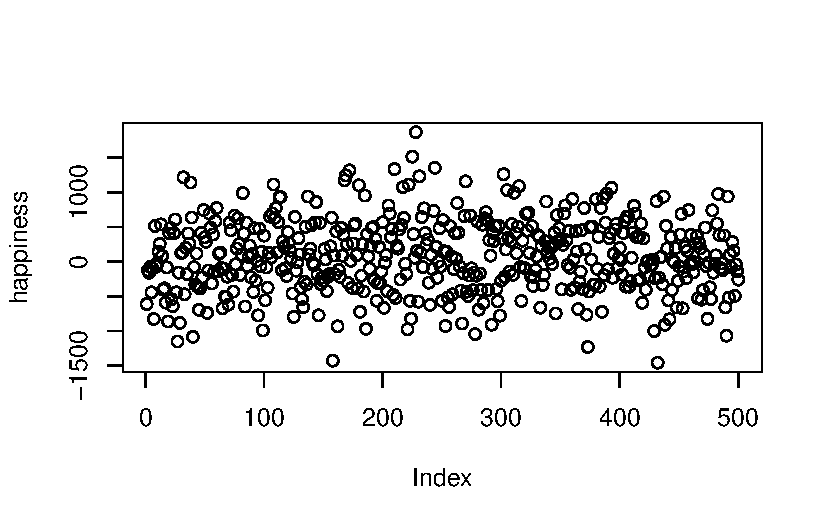
\includegraphics[width=0.75\textwidth,height=\textheight]{02-Describing_Data_files/figure-pdf/fig-happyPlot-1.pdf}

}

\caption{\label{fig-happyPlot}Pretend happiness ratings from 500 people}

\end{figure}

Figure~\ref{fig-happyPlot} shows 500 measurements of happiness. The
graph has two axes. The horizontal \textbf{x-axis}, going from left to
right is labeled ``Index''. The vertical \textbf{y-axis}, going up and
down, is labelled ``happiness''. Each dot represents one measurement of
every person's happiness from our pretend study. Before we talk about
what we can and cannot see about the data, it is worth mentioning that
the way you plot the data will make some things easier to see and some
things harder to see. So, what can we now see about the data?

There are lots of dots everywhere. It looks like there are 500 of them
because the index goes to 500. It looks like some dots go as high as
1000-1500 and as low as -1500. It looks like there are more dots in the
middle-ish area of the plot, sort of spread about 0.

\begin{quote}
Take home: we can see all the numbers at once by putting them in a plot,
and that is much easier and more helpful than looking at the raw
numbers.
\end{quote}

OK, so if these dots represent how happy 500 people are, what can we say
about those people? First, the dots are kind of all over the place, so
different people have different levels of happiness. Are there any
trends? Are more people happy than unhappy, or vice-versa? It's hard to
see that in the graph, so let's make a different one, called a
\textbf{histogram.}

\hypertarget{histograms}{%
\subsection{Histograms}\label{histograms}}

Making a histogram will be our first act of officially summarizing
something about the data. We will no longer look at the individual bits
of data, instead we will see how the numbers group together. Let's look
at Figure~\ref{fig-happyHist}, a histogram of the happiness data, and
then explain it.

\begin{figure}

{\centering 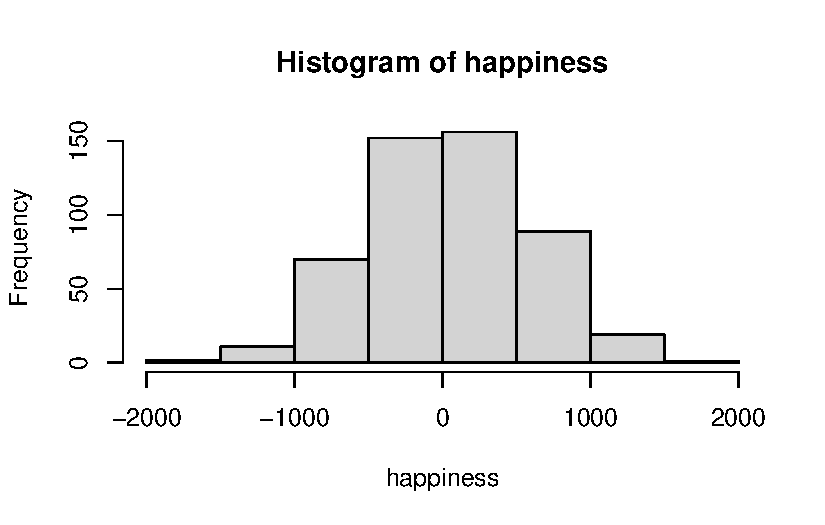
\includegraphics[width=0.75\textwidth,height=\textheight]{02-Describing_Data_files/figure-pdf/fig-happyHist-1.pdf}

}

\caption{\label{fig-happyHist}A histogram of the happiness ratings}

\end{figure}

The dots have disappeared, and now we some bars. Each bar is a summary
of the dots, representing the number of dots (frequency count) inside a
particular range of happiness, also called \textbf{bins}. For example,
how many people gave a happiness rating between 0 and 500? The fifth
bar, the one between 0 and 500 on the x-axis, tells you how many. Look
how tall that bar is. How tall is it? The height is shown on the y-axis,
which provides a frequency count (the number of dots or data points). It
looks like around 150 people said their happiness was between 0-500.

More generally, we see there are many bins on the x-axis. We have
divided the data into bins of 500. Bin \#1 goes from -2000 to -1500, bin
\#2 goes from -1500 to -1000, and so on until the last bin. To make the
histogram, we just count up the number of data points falling inside
each bin, then plot those frequency counts as a function of the bins.
Voila, a histogram.

What does the histogram help us see about the data? First, we can see
the \textbf{shape} of data. The shape of the histogram refers to how it
goes up and down. The shape tells us where the data is. For example,
when the bars are low we know there isn't much data there. When the bars
are high, we know there is more data there. So, where is most of the
data? It looks like it's mostly in the middle two bins, between -500 and
500. We can also see the \textbf{range} of the data. This tells us the
minimums and the maximums of the data. Most of the data is between -1500
and +1500, so no infinite sadness or infinite happiness in our data-set.

When you make a histogram you get to choose how wide each bar will be.
For example, below are four different histograms of the very same
happiness data. What changes is the width of the bins.

\begin{figure}

{\centering 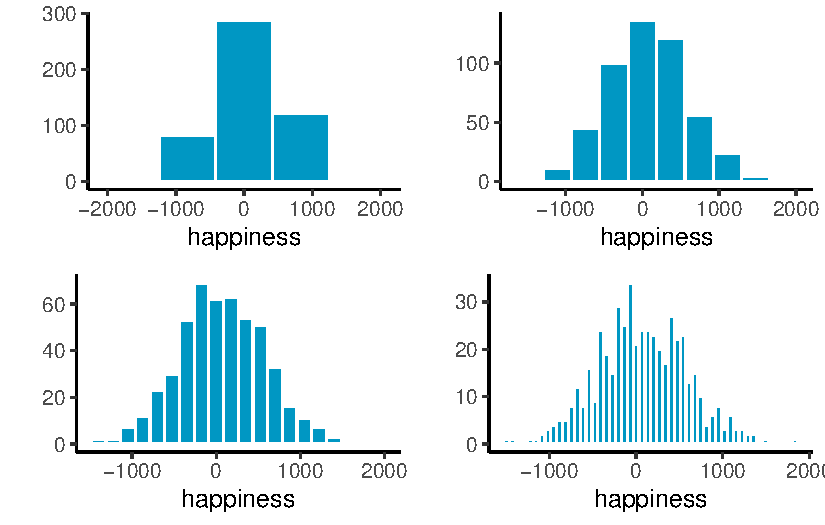
\includegraphics[width=0.75\textwidth,height=\textheight]{02-Describing_Data_files/figure-pdf/fig-manyhistbin-1.pdf}

}

\caption{\label{fig-manyhistbin}Four histograms of the same data using
different bin widths}

\end{figure}

All of the histograms have roughly the same overall shape: From left to
right, the bars start off small, then go up, then get small again. In
other words, as the numbers get closer to zero, they start to occur more
frequently. We see this general trend across all the histograms. But,
some aspects of the trend fall apart when the bars get really narrow.
For example, although the bars generally get taller when moving from
-1000 to 0, there are some exceptions and the bars seem to fluctuate a
little bit. When the bars are wider, there are less exceptions to the
general trend. How wide or narrow should your histogram be? It's a
Goldilocks question. Make it just right for your data.

\hypertarget{important-ideas-distribution-central-tendency-and-variance}{%
\section{Important Ideas: Distribution, Central Tendency, and
Variance}\label{important-ideas-distribution-central-tendency-and-variance}}

Let's introduce three important terms we will use a lot,
\textbf{distribution}, \textbf{central tendency}, and \textbf{variance}.
These terms are similar to their everyday meanings (although I suspect
most people don't say central tendency very often).

\textbf{Distribution.} When you order something from Amazon, where does
it come from, and how does it get to your place? That stuff comes from
one of Amazon's distribution centers. They distribute all sorts of
things by spreading them around to your doorstep. ``To Distribute'''' is
to spread something. Notice, the data in the histogram is distributed,
or spread across the bins. We can also talk about a distribution as a
noun. The histogram is a distribution of the frequency counts across the
bins. Distributions are \textbf{very, very, very, very, very} important.
They can have many different shapes. They can describe data, like in the
histogram above. And as we will learn in later chapters, they can
\textbf{produce} data. Many times we will be asking questions about
where our data came from, and this usually means asking what kind of
distribution could have created our data (more on that later.)

\textbf{Central Tendency} is all about sameness: What is common about
some numbers? For example, is there anything similar about all of the
numbers in the histogram? Yes, we can say that most of them are near 0.
There is a tendency for most of the numbers to be centered near 0.
Notice we are being cautious about our generalization about the numbers.
We are not saying they are all 0. We are saying there is a tendency for
many of them to be near zero. There are lots of ways to talk about the
central tendency of some numbers. There can even be more than one kind
of tendency. For example, if lots of the numbers were around -1000, and
a similar large amount of numbers were grouped around 1000, we could say
there was two tendencies.

\textbf{Variance} is all about different\emph{ness}: What is different
about some numbers?. For example, is there anything different about all
of the numbers in the histogram? YES!!! The numbers are not all the
same! When the numbers are not all the same, they must vary. So, the
variance in the numbers refers to how the numbers are different. There
are many ways to summarize the amount of variance in the numbers, and we
discuss these very soon.

\hypertarget{measures-of-central-tendency-sameness}{%
\section{Measures of Central Tendency
(Sameness)}\label{measures-of-central-tendency-sameness}}

We've seen that we can get a sense of data by plotting dots in a graph,
and by making a histogram. These tools show us what the numbers look
like, approximately how big and small they are, and how similar and
different they are from another. It is good to get a feeling about the
numbers in this way. But, these visual sensitudes are not very precise.
In addition to summarizing numbers with graphs, we can summarize numbers
using numbers (NO, please not more numbers, we promise numbers can be
your friend).

\hypertarget{from-many-numbers-to-one}{%
\subsection{From many numbers to one}\label{from-many-numbers-to-one}}

Measures of central have one important summary goal: to reduce a pile of
numbers to a single number that we can look at. We already know that
looking at thousands of numbers is hopeless. Wouldn't it be nice if we
could just look at one number instead? We think so. It turns out there
are lots of ways to do this. Then, if your friend ever asks the
frightening question, ``hey, what are all these numbers like?''. You can
say they are like this one number right here.

But, just like in Indiana Jones and the Last Crusade (highly recommended
movie), you must choose your measure of central tendency wisely.

\hypertarget{mode}{%
\subsection{Mode}\label{mode}}

The \textbf{mode} is the most frequently occurring number in your
measurement. That is it. How do you find it? You have to count the
number of times each number appears in your measure, then whichever one
occurs the most, is the mode.

\begin{quote}
Example: 1 1 1 2 3 4 5 6
\end{quote}

The mode of the above set is 1, which occurs three times. Every other
number only occurs once.

OK fine. What happens here:

\begin{quote}
Example: 1 1 1 2 2 2 3 4 5 6
\end{quote}

Hmm, now 1 and 2 both occur three times each. What do we do? We say
there are two modes, and they are 1 and 2.

Why is the mode a measure of central tendency? Well, when we ask, ``what
are my numbers like'', we can say, ``most of the number are, like a 1
(or whatever the mode is)''.

Is the mode a good measure of central tendency? That depends on your
numbers. For example, consider these numbers

\begin{quote}
1 1 2 3 4 5 6 7 8 9
\end{quote}

Here, the mode is 1 again, because there are two 1s, and all of the
other numbers occur once. But, are most of the numbers like, a 1. No,
they are mostly not 1s.

``Argh, so should I or should I not use the mode? I thought this class
was supposed to tell me what to do?''. There is no telling you what to
do. Every time you use a tool in statistics you have to think about what
you are doing and justify why what you are doing makes sense. Sorry.

\hypertarget{median}{%
\subsection{Median}\label{median}}

The \textbf{median} is the exact middle of the data. After all, we are
asking about central tendency, so why not go to the center of the data
and see where we are. What do you mean middle of the data? Let's look at
these numbers:

\begin{quote}
1 5 4 3 6 7 9
\end{quote}

Umm, OK. So, three is in the middle? Isn't that kind of arbitrary. Yes.
Before we can compute the median, we need to order the numbers from
smallest to largest.

\begin{quote}
1 3 4 \textbf{5} 6 7 9
\end{quote}

Now, 5 is in the middle. And, by middle we mean in the middle. There are
three numbers to the left of 5, and three numbers to the right. So, five
is definitely in the middle.

OK fine, but what happens when there aren't an even number of numbers?
Then the middle will be missing right? Let's see:

\begin{quote}
1 2 3 4 5 6
\end{quote}

There is no number between 3 and 4 in the data, the middle is empty. In
this case, we compute the median by figuring out the number in between 3
and 4. So, the median would be 3.5.

Is the median a good measure of central tendency? Sure, it is often very
useful. One property of the median is that it stays in the middle even
when some of the other numbers get really weird. For example, consider
these numbers:

\begin{quote}
1 2 3 4 4 4 \textbf{5} 6 6 6 7 7 1000
\end{quote}

Most of these numbers are smallish, but the 1000 is a big old weird
number, very different from the rest. The median is still 5, because it
is in the middle of these ordered numbers. We can also see that five is
pretty similar to most of the numbers (except for 1000). So, the median
does a pretty good job of representing most of the numbers in the set,
and it does so even if one or two of the numbers are very different from
the others.

Finally, \textbf{outlier} is a term will we use to describe numbers that
appear in data that are very different from the rest. 1000 is an
outlier, because it lies way out there on the number line compared to
the other numbers. What to do with outliers is another topic we discuss
sometimes throughout this course.

\hypertarget{mean}{%
\subsection{Mean}\label{mean}}

Have you noticed this is a textbook about statistics that hasn't used a
formula yet? That is about to change, but for those of you with formula
anxiety, don't worry, we will do our best to explain them.

The \textbf{mean} is also called the average. And, we're guessing you
might already now what the average of a bunch of numbers is? It's the
sum of the numbers, divided by the number of number right? How do we
express that idea in a formula? Just like this:

\(Mean = \bar{X} = \frac{\sum_{i=1}^{n} x_{i}}{N}\)

``That looks like Greek to me''. Yup. The \(\sum\) symbol is called
\textbf{sigma}, and it stands for the operation of summing. The little
``i'' on the bottom, and the little ``n'' on the top refers to all of
the numbers in the set, from the first number ``i'' to the last number
``n''. The letters are just arbitrary labels, called \textbf{variables}
that we use for descriptive purposes. The \(x_{i}\) refers to individual
numbers in the set. We sum up all of the numbers, then divide the sum by
\(N\), which is the total number of numbers. Sometimes you will see
\(\bar{X}\) to refer to the mean of all of the numbers.

In plain English, the formula looks like:

\(mean = \frac{\text{Sum of my numbers}}{\text{Count of my numbers}}\)

``Well, why didn't you just say that?''. We just did.

Let's compute the mean for these five numbers:

\begin{quote}
3 7 9 2 6
\end{quote}

Add em up:

\begin{quote}
3+7+9+2+6 = 27
\end{quote}

Count em up:

\begin{quote}
\(i_{1}\) = 3, \(i_{2}\) = 7, \(i_{3}\) = 9, \(i_{4}\) = 2, \(i_{5}\) =
6; N=5, because \(i\) went from 1 to 5
\end{quote}

Divide em:

\begin{quote}
mean = 27 / 5 = 5.4
\end{quote}

Or, to put the numbers in the formula, it looks like this:

\(Mean = \bar{X} = \frac{\sum_{i=1}^{n} x_{i}}{N} = \frac{3+7+9+2+6}{5} = \frac{27}{5} = 5.4\)

OK fine, that is how to compute the mean. But, like we imagined, you
probably already knew that, and if you didn't that's OK, now you do.
What's next?

Is the mean a good measure of central tendency? By now, you should know:
it depends.

\hypertarget{what-does-the-mean-mean}{%
\subsection{What does the mean mean?}\label{what-does-the-mean-mean}}

It is not enough to know the formula for the mean, or to be able to use
the formula to compute a mean for a set of numbers. We believe in your
ability to add and divide numbers. What you really need to know is what
the mean really ``means''. This requires that you know what the mean
does, and not just how to do it. Puzzled? Let's explain.

Can you answer this question: What happens when you divide a sum of
numbers by the number of numbers? What are the consequences of doing
this? What is the formula doing? What kind of properties does the result
give us? FYI, the answer is not that we compute the mean.

OK, so what happens when you divide any number by another number? Of
course, the key word here is divide. We literally carve the number up
top in the numerator into pieces. How many times do we split the top
number? That depends on the bottom number in the denominator. Watch:

\(\frac{12}{3} = 4\)

So, we know the answer is 4. But, what is really going on here is that
we are slicing and dicing up 12 aren't we. Yes, and we slicing 12 into
three parts. It turns out the size of those three parts is 4. So, now we
are thinking of 12 as three different pieces \(12 = 4 + 4 + 4\). I know
this will be obvious, but what kind of properties do our pieces have?
You mean the fours? Yup. Well, obviously they are all fours. Yes. The
pieces are all the same size. They are all equal. So, division equalizes
the numerator by the denominator\ldots{}

``Umm, I think I learned this in elementary school, what does this have
to do with the mean?''. The number on top of the formula for the mean is
just another numerator being divided by a denominator isn't it. In this
case, the numerator is a sum of all the values in your data. What if it
was the sum of all of the 500 happiness ratings? The sum of all of them
would just be a single number adding up all the different ratings. If we
split the sum up into equal parts representing one part for each
person's happiness what would we get? We would get 500 identical and
equal numbers for each person. It would be like taking all of the
happiness in the world, then dividing it up equally, then to be fair,
giving back the same equal amount of happiness to everyone in the world.
This would make some people more happy than they were before, and some
people less happy right. Of course, that's because it would be
equalizing the distribution of happiness for everybody. This process of
equalization by dividing something into equal parts is what the
\textbf{mean} does. See, it's more than just a formula. It's an idea.
This is just the beginning of thinking about these kinds of ideas. We
will come back to this idea about the mean, and other ideas, in later
chapters.

\begin{quote}
Pro tip: The mean is the one and only number that can take the place of
every number in the data, such that when you add up all the equal parts,
you get back the original sum of the data.
\end{quote}

\hypertarget{all-together-now}{%
\subsection{All together now}\label{all-together-now}}

Just to remind ourselves of the mode, median, and mean, take a look at
the next histogram in Figure~\ref{fig-meanmodemed}. We have overlaid the
location of the mean (red), median (green), and mode (blue). For this
dataset, the three measures of central tendency all give different
answers. The mean is the largest because it is influenced by large
numbers, even if they occur rarely. The mode and median are insensitive
to large numbers that occur infrequently, so they have smaller values.

\begin{figure}

{\centering 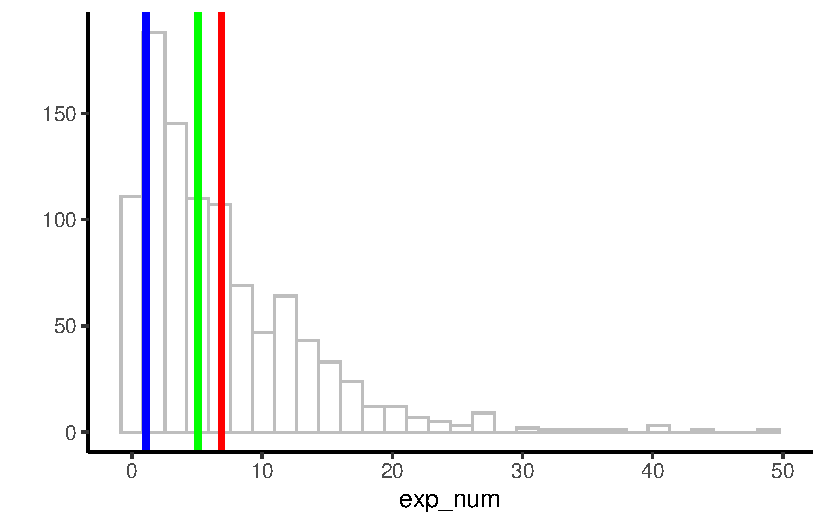
\includegraphics[width=0.75\textwidth,height=\textheight]{02-Describing_Data_files/figure-pdf/fig-meanmodemed-1.pdf}

}

\caption{\label{fig-meanmodemed}A histogram with the mean (red), the
median (green), and the mode (blue)}

\end{figure}

\hypertarget{measures-of-variation-differentness}{%
\section{\texorpdfstring{Measures of Variation
(Different\emph{ness})}{Measures of Variation (Differentness)}}\label{measures-of-variation-differentness}}

What did you do when you wrote essays in high school about a book you
read? Probably compare and contrast something right? When you summarize
data, you do the same thing. Measures of central tendency give us
something like comparing does, they tell us stuff about what is the
same. Measures of variation give us something like contrasting does,
they tell us stuff about what is different.

First, we note that whenever you see a bunch of numbers that aren't the
same, you already know there are some differences. This means the
numbers vary, and there is variation in the size of the numbers.

\hypertarget{the-range}{%
\subsection{The Range}\label{the-range}}

Consider these 10 numbers, that I already ordered from smallest to
largest for you:

\begin{quote}
1 3 4 5 5 6 7 8 9 24
\end{quote}

The numbers have variation, because they are not all the same. We can
use the range to describe the width of the variation. The range refers
to the \textbf{minimum} (smallest value) and \textbf{maximum} (largest
value) in the set. So, the range would be 1 and 24.

The range is a good way to quickly summarize the boundaries of your data
in just two numbers. By computing the range we know that none of the
data is larger or smaller than the range. And, it can alert you to
outliers. For example, if you are expecting your numbers to be between 1
and 7, but you find the range is 1 - 340,500, then you know you have
some big numbers that shouldn't be there, and then you can try to figure
out why those numbers occurred (and potentially remove them if something
went wrong).

\hypertarget{the-difference-scores}{%
\subsection{The Difference Scores}\label{the-difference-scores}}

It would be nice to summarize the amount of different\emph{ness} in the
data. Here's why. If you thought that raw data (lots of numbers) is too
big to look at, then you will be frightened to contemplate how many
differences there are to look at. For example, these 10 numbers are easy
to look at:

\begin{quote}
1 3 4 5 5 6 7 8 9 24
\end{quote}

But, what about the difference between the numbers, what do those look
like? We can compute the difference scores between each number, then put
them in a matrix like the one below:

\begin{longtable}[]{@{}lrrrrrrrrrr@{}}
\toprule\noalign{}
& 1 & 3 & 4 & 5 & 5 & 6 & 7 & 8 & 9 & 24 \\
\midrule\noalign{}
\endhead
\bottomrule\noalign{}
\endlastfoot
1 & 0 & 2 & 3 & 4 & 4 & 5 & 6 & 7 & 8 & 23 \\
3 & -2 & 0 & 1 & 2 & 2 & 3 & 4 & 5 & 6 & 21 \\
4 & -3 & -1 & 0 & 1 & 1 & 2 & 3 & 4 & 5 & 20 \\
5 & -4 & -2 & -1 & 0 & 0 & 1 & 2 & 3 & 4 & 19 \\
5 & -4 & -2 & -1 & 0 & 0 & 1 & 2 & 3 & 4 & 19 \\
6 & -5 & -3 & -2 & -1 & -1 & 0 & 1 & 2 & 3 & 18 \\
7 & -6 & -4 & -3 & -2 & -2 & -1 & 0 & 1 & 2 & 17 \\
8 & -7 & -5 & -4 & -3 & -3 & -2 & -1 & 0 & 1 & 16 \\
9 & -8 & -6 & -5 & -4 & -4 & -3 & -2 & -1 & 0 & 15 \\
24 & -23 & -21 & -20 & -19 & -19 & -18 & -17 & -16 & -15 & 0 \\
\end{longtable}

We are looking at all of the possible differences between each number
and every other number. So, in the top left, the difference between 1
and itself is 0. One column over to the right, the difference between 3
and 1 (3-1) is 2, etc. As you can see, this is a 10x10 matrix, which
means there are 100 differences to look at. Not too bad, but if we had
500 numbers, then we would have 500*500 = 250,000 differences to look at
(go for it if you like looking at that sort of thing).

Pause for a simple question. What would this matrix look like if all of
the 10 numbers in our data were the same number? It should look like a
bunch of 0s right? Good. In that case, we could easily see that the
numbers have no variation.

But, when the numbers are different, we can see that there is a very
large matrix of difference scores. How can we summarize that? How about
we apply what we learned from the previous section on measures of
central tendency. We have a lot of differences, so we could ask
something like, what is the average difference that we have? So, we
could just take all of our differences, and compute the mean difference
right? What do you think would happen if we did that?

Let's try it out on these three numbers:

\begin{quote}
1 2 3
\end{quote}

\begin{longtable}[]{@{}lrrr@{}}
\toprule\noalign{}
& 1 & 2 & 3 \\
\midrule\noalign{}
\endhead
\bottomrule\noalign{}
\endlastfoot
1 & 0 & 1 & 2 \\
2 & -1 & 0 & 1 \\
3 & -2 & -1 & 0 \\
\end{longtable}

You might already guess what is going to happen. Let's compute the mean:

\(\text{mean of difference scores} = \frac{0+1+2-1+0+1-2-1+0}{9} = \frac{0}{9} = 0\)

Uh oh, we get zero for the mean of the difference scores. This will
always happen whenever you take the mean of the difference scores. We
can see that there are some differences between the numbers, so using 0
as the summary value for the variation in the numbers doesn't make much
sense.

Furthermore, you might also notice that the matrices of difference
scores are redundant. The diagonal is always zero, and numbers on one
side of the diagonal are the same as the numbers on the other side,
except their signs are reversed. So, that's one reason why the
difference scores add up to zero.

These are little problems that can be solved by computing the
\textbf{variance} and the \textbf{standard deviation}. For now, the
standard deviation is a just a trick that we use to avoid getting a
zero. But, later we will see it has properties that are important for
other reasons.

\hypertarget{the-variance}{%
\subsection{The Variance}\label{the-variance}}

Variability, variation, variance, vary, variable, varying, variety.
Confused yet? Before we describe \textbf{the variance}, we want to you
be OK with how this word is used. First, don't forget the big picture.
We know that variability and variation refers to the big idea of
differences between numbers. We can even use the word variance in the
same way. When numbers are different, they have variance.

\begin{tcolorbox}[enhanced jigsaw, breakable, colback=white, coltitle=black, toptitle=1mm, rightrule=.15mm, title=\textcolor{quarto-callout-note-color}{\faInfo}\hspace{0.5em}{Note}, opacitybacktitle=0.6, opacityback=0, colframe=quarto-callout-note-color-frame, leftrule=.75mm, colbacktitle=quarto-callout-note-color!10!white, arc=.35mm, bottomtitle=1mm, titlerule=0mm, bottomrule=.15mm, toprule=.15mm, left=2mm]

The formulas for variance and standard deviation depend on whether you
think your data represents an entire population of numbers, or is sample
from the population. We discuss this issue in later on. For now, we
divide by N, later we discuss why you will often divide by N-1 instead.

\end{tcolorbox}

The word \textbf{variance} also refers to a specific summary statistic,
the sum of the squared deviations from the mean. Hold on what? Plain
English please. The variance is the sum of the squared difference
scores, where the difference scores are computed between each score and
the mean. What are these scores? The scores are the numbers in the data
set. Let's see the formula in English first:

\(variance = \frac{\text{Sum of squared difference scores}}{\text{Number of Scores}}\)

\hypertarget{deviations-from-the-mean-difference-scores-from-the-mean}{%
\subsubsection{Deviations from the mean, Difference scores from the
mean}\label{deviations-from-the-mean-difference-scores-from-the-mean}}

We got a little bit complicated before when we computed the difference
scores between all of the numbers in the data. Let's do it again, but in
a more manageable way. This time, we calculate the difference between
each score and the mean. The idea here is

\begin{enumerate}
\def\labelenumi{\arabic{enumi}.}
\tightlist
\item
  We can figure out how similar our scores are by computing the mean
\item
  Then we can figure out how different our scores are from the mean
\end{enumerate}

This could tell us, 1) something about whether our scores are really all
very close to the mean (which could help us know if the mean is good
representative number of the data), and 2) something about how much
differences there are in the numbers.

Take a look at this table:

\begin{longtable}[]{@{}llll@{}}
\toprule\noalign{}
scores & values & mean & Difference\_from\_Mean \\
\midrule\noalign{}
\endhead
\bottomrule\noalign{}
\endlastfoot
1 & 1 & 4.5 & -3.5 \\
2 & 6 & 4.5 & 1.5 \\
3 & 4 & 4.5 & -0.5 \\
4 & 2 & 4.5 & -2.5 \\
5 & 6 & 4.5 & 1.5 \\
6 & 8 & 4.5 & 3.5 \\
Sums & 27 & 27 & 0 \\
Means & 4.5 & 4.5 & 0 \\
\end{longtable}

The first column shows we have 6 scores in the data set, and the
\texttt{value} columns shows each score. The sum of the values, and the
mean is presented on the last two rows. The sum and the mean were
obtained by:

\(\frac{1+6+4+2+6+8}{6} = \frac{27}{6} = 4.5\).

The third column \texttt{mean}, appears a bit silly. We are just listing
the mean once for every score. If you think back to our discussion about
the meaning of the mean, then you will remember that it equally
distributes the total sum across each data point. We can see that here,
if we treat each score as the mean, then every score is a 4.5. We can
also see that adding up all of the means for each score gives us back
27, which is the sum of the original values. Also, we see that if we
find the mean of the mean scores, we get back the mean (4.5 again).

All of the action is occurring in the fourth column,
\texttt{Difference\_from\_Mean}. Here, we are showing the difference
scores from the mean, using \(X_{i}-\bar{X}\). In other words, we
subtracted the mean from each score. So, the first score, 1, is -3.5
from the mean, the second score, 6, is +1.5 from the mean, and so on.

Now, we can look at our original scores and we can look at their
differences from the mean. Notice, we don't have a matrix of raw
difference scores, so it is much easier to look at out. But, we still
have a problem:

We can see that there are non-zero values in the difference scores, so
we know there are a differences in the data. But, when we add them all
up, we still get zero, which makes it seem like there are a total of
zero differences in the data\ldots Why does this happen\ldots and what
to do about it?

\hypertarget{the-mean-is-the-balancing-point-in-the-data}{%
\subsubsection{The mean is the balancing point in the
data}\label{the-mean-is-the-balancing-point-in-the-data}}

One brief pause here to point out another wonderful property of the
mean. It is the balancing point in the data. If you take a pen or pencil
and try to balance it on your figure so it lays flat what are you doing?
You need to find the center of mass in the pen, so that half of it is on
one side, and the other half is on the other side. That's how balancing
works. One side = the other side.

We can think of data as having mass or weight to it. If we put our data
on our bathroom scale, we could figure out how heavy it was by summing
it up. If we wanted to split the data down the middle so that half of
the weight was equal to the other half, then we could balance the data
on top of a pin. The mean of the data tells you where to put the pin. It
is the location in the data, where the numbers on the one side add up to
the same sum as the numbers on the other side.

If we think this through, it means that the sum of the difference scores
from the mean will always add up to zero. This is because the numbers on
one side of the mean will always add up to -x (whatever the sum of those
numbers is), and the numbers of the other side of the mean will always
add up to +x (which will be the same value only positive). And:

\(-x + x = 0\), right.

Right.

\hypertarget{the-squared-deviations}{%
\subsubsection{The squared deviations}\label{the-squared-deviations}}

Some devious someone divined a solution to the fact that differences
scores from the mean always add to zero. Can you think of any solutions?
For example, what could you do to the difference scores so that you
could add them up, and they would weigh something useful, that is they
would not be zero?

The devious solution is to square the numbers. Squaring numbers converts
all the negative numbers to positive numbers. For example, \(2^2 = 4\),
and \(-2^2 = 4\). Remember how squaring works, we multiply the number
twice: \(2^2 = 2*2 = 4\), and \(-2^2 = -2*-2 = 4\). We use the term
\textbf{squared deviations} to refer to differences scores that have
been squared. Deviations are things that move away from something. The
difference scores move away from the mean, so we also call them
\textbf{deviations}.

Let's look at our table again, but add the squared deviations.

\begin{longtable}[]{@{}lllll@{}}
\toprule\noalign{}
scores & values & mean & Difference\_from\_Mean & Squared\_Deviations \\
\midrule\noalign{}
\endhead
\bottomrule\noalign{}
\endlastfoot
1 & 1 & 4.5 & -3.5 & 12.25 \\
2 & 6 & 4.5 & 1.5 & 2.25 \\
3 & 4 & 4.5 & -0.5 & 0.25 \\
4 & 2 & 4.5 & -2.5 & 6.25 \\
5 & 6 & 4.5 & 1.5 & 2.25 \\
6 & 8 & 4.5 & 3.5 & 12.25 \\
Sums & 27 & 27 & 0 & 35.5 \\
Means & 4.5 & 4.5 & 0 & 5.91666666666667 \\
\end{longtable}

OK, now we have a new column called \texttt{squared\_deviations}. These
are just the difference scores squared. So, \(-3.5^2 = 12.25\), etc. You
can confirm for yourself with your cellphone calculator.

Now that all of the squared deviations are positive, we can add them up.
When we do this we create something very special called the sum of
squares (SS), also known as the sum of the squared deviations from the
mean. We will talk at length about this SS later on in the ANOVA
chapter. So, when you get there, remember that you already know what it
is, just some sums of some squared deviations, nothing fancy.

\hypertarget{finally-the-variance}{%
\subsubsection{Finally, the variance}\label{finally-the-variance}}

Guess what, we already computed the variance. It already happened, and
maybe you didn't notice. ``Wait, I missed that, what happened?''.

First, see if you can remember what we are trying to do here. Take a
pause, and see if you can tell yourself what problem we are trying
solve.

\begin{quote}
pause
\end{quote}

Without further ado, we are trying to get a summary of the differences
in our data. There are just as many difference scores from the mean as
there are data points, which can be a lot, so it would be nice to have a
single number to look at, something like a mean, that would tell us
about the average differences in the data.

If you look at the table, you can see we already computed the mean of
the squared deviations. First, we found the sum (SS), then below that we
calculated the mean = 5.916 repeating. This is \textbf{the variance}.
The variance is the mean of the sum of the squared deviations:

\(variance = \frac{SS}{N}\), where SS is the sum of the squared
deviations, and N is the number of observations.

OK, now what. What do I do with the variance? What does this number
mean? Good question. The variance is often an unhelpful number to look
at. Why? Because it is not in the same scale as the original data. This
is because we squared the difference scores before taking the mean.
Squaring produces large numbers. For example, we see a 12.25 in there.
That's a big difference, bigger than any difference between any two
original values. What to do? How can we bring the numbers back down to
their original unsquared size?

If you are thinking about taking the square root, that's a ding ding
ding, correct answer for you. We can always unsquare anything by taking
the square root. So, let's do that to 5.916. \(\sqrt{5.916} =\)
2.4322829.

\hypertarget{the-standard-deviation}{%
\subsection{The Standard Deviation}\label{the-standard-deviation}}

Oops, we did it again. We already computed the standard deviation, and
we didn't tell you. The standard deviation is the square root of the
variance\ldots At least, it is right now, until we complicate matters
for you in the next chapter.

Here is the formula for the standard deviation:

\(\text{standard deviation} = \sqrt{Variance} = \sqrt{\frac{SS}{N}}\).

We could also expand this to say:

\(\text{standard deviation} = \sqrt{\frac{\sum_{i}^{n}({x_{i}-\bar{x})^2}}{N}}\)

Don't let those big square root signs put you off. Now, you know what
they are doing there. Just bringing our measure of the variance back
down to the original size of the data. Let's look at our table again:

\begin{longtable}[]{@{}lllll@{}}
\toprule\noalign{}
scores & values & mean & Difference\_from\_Mean & Squared\_Deviations \\
\midrule\noalign{}
\endhead
\bottomrule\noalign{}
\endlastfoot
1 & 1 & 4.5 & -3.5 & 12.25 \\
2 & 6 & 4.5 & 1.5 & 2.25 \\
3 & 4 & 4.5 & -0.5 & 0.25 \\
4 & 2 & 4.5 & -2.5 & 6.25 \\
5 & 6 & 4.5 & 1.5 & 2.25 \\
6 & 8 & 4.5 & 3.5 & 12.25 \\
Sums & 27 & 27 & 0 & 35.5 \\
Means & 4.5 & 4.5 & 0 & 5.91666666666667 \\
\end{longtable}

We measured the standard deviation as 2.4322829. Notice this number fits
right in the with differences scores from the mean. All of the scores
are kind of in and around + or - 2.4322829. Whereas, if we looked at the
variance, 5.916 is just too big, it doesn't summarize the actual
differences very well.

What does all this mean? Well, if someone told they had some number with
a mean of 4.5 (like the values in our table), and a standard deviation
of 2.4322829, you would get a pretty good summary of the numbers. You
would know that many of the numbers are around 4.5, and you would know
that not all of the numbers are 4.5. You would know that the numbers
spread around 4.5. You also know that the spread isn't super huge, it's
only + or - 2.4322829 on average. That's a good starting point for
describing numbers.

If you had loads of numbers, you could reduce them down to the mean and
the standard deviation, and still be pretty well off in terms of getting
a sense of those numbers.

\hypertarget{using-descriptive-statistics-with-data}{%
\section{Using Descriptive Statistics with
data}\label{using-descriptive-statistics-with-data}}

Remember, you will be learning how to compute descriptive statistics
using software in the labs. Check out the
\href{https://crumplab.github.io/statisticsLab/lab-2-descriptive-statistics.html}{lab
manual exercises for descriptives} to see some examples of working with
real data.

\hypertarget{rolling-your-own-descriptive-statistics}{%
\section{Rolling your own descriptive
statistics}\label{rolling-your-own-descriptive-statistics}}

We spent many paragraphs talking about variation in numbers, and how to
use calculate the \textbf{variance} and \textbf{standard deviation} to
summarize the average differences between numbers in a data set. The
basic process was to 1) calculate some measure of the differences, then
2) average the differences to create a summary. We found that we
couldn't average the raw difference scores, because we would always get
a zero. So, we squared the differences from the mean, then averaged the
squared differences differences. Finally, we square rooted our measure
to bring the summary back down to the scale of the original numbers.

Perhaps you haven't heard, but there is more than one way to skin a cat,
but we prefer to think of this in terms of petting cats, because some of
us love cats. Jokes aside, perhaps you were also thinking that the
problem of summing differences scores (so that they don't equal zero),
can be solved in more than one way. Can you think of a different way,
besides squaring?

\hypertarget{absolute-deviations}{%
\subsection{Absolute deviations}\label{absolute-deviations}}

How about just taking the absolute value of the difference scores.
Remember, the absolute value converts any number to a positive value.
Check out the following table:

\begin{longtable}[]{@{}lllll@{}}
\toprule\noalign{}
scores & values & mean & Difference\_from\_Mean &
Absolute\_Deviations \\
\midrule\noalign{}
\endhead
\bottomrule\noalign{}
\endlastfoot
1 & 1 & 4.5 & -3.5 & 3.5 \\
2 & 6 & 4.5 & 1.5 & 1.5 \\
3 & 4 & 4.5 & -0.5 & 0.5 \\
4 & 2 & 4.5 & -2.5 & 2.5 \\
5 & 6 & 4.5 & 1.5 & 1.5 \\
6 & 8 & 4.5 & 3.5 & 3.5 \\
Sums & 27 & 27 & 0 & 13 \\
Means & 4.5 & 4.5 & 0 & 2.16666666666667 \\
\end{longtable}

This works pretty well too. By converting the difference scores from the
mean to positive values, we can now add them up and get a non-zero value
(if there are differences). Then, we can find the mean of the sum of the
absolute deviations. If we were to map the terms sum of squares (SS),
variance and standard deviation onto these new measures based off of the
absolute deviation, how would the mapping go? For example, what value in
the table corresponds to the SS? That would be the sum of absolute
deviations in the last column. How about the variance and standard
deviation, what do those correspond to? Remember that the variance is
mean (\(SS/N\)), and the standard deviation is a square-rooted mean
(\(\sqrt{SS/N}\)). In the table above we only have one corresponding
mean, the mean of the sum of the absolute deviations. So, we have a
\textbf{variance} measure that does not need to be square rooted. We
might say the mean absolute deviation, is doing double-duty as a
variance and a standard-deviation. Neat.

\hypertarget{other-sign-inverting-operations}{%
\subsection{Other sign-inverting
operations}\label{other-sign-inverting-operations}}

In principle, we could create lots of different summary statistics for
variance that solve the summing to zero problem. For example, we could
raise every difference score to any even numbered power beyond 2 (which
is the square). We could use, 4, 6, 8, 10, etc. There is an infinity of
even numbers, so there is an infinity of possible variance statistics.
We could also use odd numbers as powers, and then take their absolute
value. Many things are possible. The important aspect to any of this is
to have a reason for what you are doing, and to choose a method that
works for the data-analysis problem you are trying to solve. Note also,
we bring up this general issue because we want you to understand that
statistics is a creative exercise. We invent things when we need them,
and we use things that have already been invented when they work for the
problem at hand.

\hypertarget{remember-to-look-at-your-data}{%
\section{Remember to look at your
data}\label{remember-to-look-at-your-data}}

Descriptive statistics are great and we will use them a lot in the
course to describe data. You may suspect that descriptive statistics
also have some short-comings. This is very true. They are compressed
summaries of large piles of numbers. They will almost always be unable
to represent all of the numbers fairly. There are also different kinds
of descriptive statistics that you could use, and it sometimes not clear
which one's you should use.

Perhaps the most important thing you can do when using descriptives is
to use them in combination with looking at the data in a graph form.
This can help you see whether or not your descriptives are doing a good
job of representing the data.

\hypertarget{anscombes-quartet}{%
\subsection{Anscombe's Quartet}\label{anscombes-quartet}}

To hit this point home, and to get you thinking about the issues we
discuss in the next chapter, check this out. It's called Anscombe's
Quartet, because these interesting graphs and numbers and numbers were
produced by Anscombe (1973). In Figure~\ref{fig-anscombe} you are
looking at pairs of measurements. Each graph has an X and Y axis, and
each point represents two measurements. Each of the graphs looks very
different, right?

\begin{figure}

{\centering 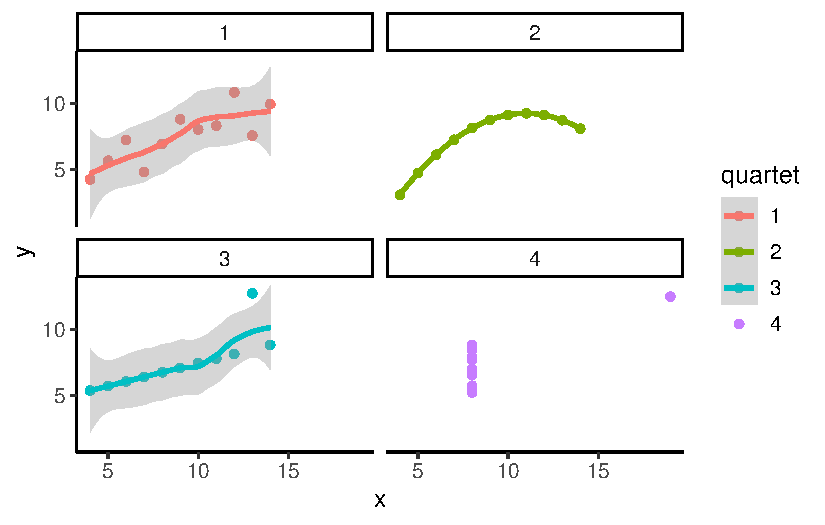
\includegraphics[width=0.75\textwidth,height=\textheight]{02-Describing_Data_files/figure-pdf/fig-anscombe-1.pdf}

}

\caption{\label{fig-anscombe}Anscombe's Quartet}

\end{figure}

Well, would you be surprised if I told that the descriptive statistics
for the numbers in these graphs are exactly the same? It turns out they
do have the same descriptive statistics. In the table below I present
the mean and variance for the x-values in each graph, and the mean and
the variance for the y-values in each graph.

\begin{longtable}[]{@{}lrrrr@{}}
\toprule\noalign{}
quartet & mean\_x & var\_x & mean\_y & var\_y \\
\midrule\noalign{}
\endhead
\bottomrule\noalign{}
\endlastfoot
1 & 9 & 11 & 7.500909 & 4.127269 \\
2 & 9 & 11 & 7.500909 & 4.127629 \\
3 & 9 & 11 & 7.500000 & 4.122620 \\
4 & 9 & 11 & 7.500909 & 4.123249 \\
\end{longtable}

The descriptives are all the same! Anscombe put these special numbers
together to illustrate the point of graphing your numbers. If you only
look at your descriptives, you don't know what patterns in the data they
are hiding. If you look at the graph, then you can get a better
understanding.

\hypertarget{datasaurus-dozen}{%
\subsection{Datasaurus Dozen}\label{datasaurus-dozen}}

If you thought that Anscombe's quartet was neat, you should take a look
at the
\href{https://www.autodeskresearch.com/publications/samestats}{Datasaurus
Dozen} (Matejka and Fitzmaurice 2017). Scroll down to see the examples.
You will be looking at dot plots. The dot plots show many different
patterns, including dinosaurs! What's amazing is that all of the dots
have very nearly the same descriptive statistics. Just another reminder
to look at your data, it might look like a dinosaur!

\hypertarget{videos-1}{%
\section{Videos}\label{videos-1}}

\hypertarget{measures-of-center-mode}{%
\subsection{Measures of center: Mode}\label{measures-of-center-mode}}

\hypertarget{measures-of-center-median-and-mean}{%
\subsection{Measures of center: Median and
Mean}\label{measures-of-center-median-and-mean}}

\hypertarget{standard-deviation-part-i}{%
\subsection{Standard deviation part I}\label{standard-deviation-part-i}}

\hypertarget{standard-deviation-part-ii}{%
\subsection{Standard deviation part
II}\label{standard-deviation-part-ii}}

\bookmarksetup{startatroot}

\hypertarget{Correlation}{%
\chapter{Correlation}\label{Correlation}}

\begin{quote}
Correlation does not equal causation ---Every Statistics and Research
Methods Instructor Ever
\end{quote}

In the last chapter we had some data. It was too much too look at and it
didn't make sense. So, we talked about how to look at the data visually
using plots and histograms, and we talked about how to summarize lots of
numbers so we could determine their central tendencies (sameness) and
variability (differentness). And, all was well with the world.

Let's not forget the big reason why we learned about descriptive
statistics. The big reason is that we are interested in getting answers
to questions using data.

If you are looking for a big theme to think about while you take this
course, the theme is: how do we ask and answer questions using data?

For every section in this book, you should be connecting your inner
monologue to this question, and asking yourself: How does what I am
learning about help me answer questions with data? Advance warning: we
know it is easy to forget this stuff when we dive into the details, and
we will try to throw you a rope to help you out along the
way\ldots remember, we're trying to answer questions with data.

We started Chapter two with some fake data on human happiness, remember?
We imagined that we asked a bunch of people to tell us how happy they
were, then we looked at the numbers they gave us. Let's continue with
this imaginary thought experiment.

What do you get when you ask people to use a number to describe how
happy they are? A bunch of numbers. What kind of questions can you ask
about those numbers? Well, you can look at the numbers and estimate
their general properties as we already did. We would expect those
numbers tell us some things we already know. There are different people,
and different people are different amounts of happy. You've probably met
some of those of really happy people, and really unhappy people, and you
yourself probably have some amount of happiness. ``Great, thanks Captain
Obvious''.

Before moving on, you should also be skeptical of what the numbers might
mean. For example, if you force people to give a number between 0-100 to
rate their happiness, does this number truly reflect how happy that
person is? Can a person know how happy they are? Does the question
format bias how they give their answer? Is happiness even a real thing?
These are all good questions about the \textbf{validity} of the
construct (happiness itself) and the measure (numbers) you are using to
quantify it. For now, though, we will side-step those very important
questions, and assume that, happiness is a thing, and our measure of
happiness measures something about how happy people are.

OK then, after we have measured some happiness, I bet you can think of
some more pressing questions. For example, what causes happiness to go
up or down. If you knew the causes of happiness what could you do? How
about increase your own happiness; or, help people who are unhappy; or,
better appreciate why Eeyore from Winnie the Pooh is unhappy; or,
present valid scientific arguments that argue against incorrect claims
about what causes happiness. A causal theory and understanding of
happiness could be used for all of those things. How can we get there?

Imagine you were an alien observer. You arrived on earth and heard about
this thing called happiness that people have. You want to know what
causes happiness. You also discover that planet earth has lots of other
things. Which of those things, you wonder, cause happiness? How would
your alien-self get started on this big question.

As a person who has happiness, you might already have some hunches about
what causes changes in happiness. For example things like: weather,
friends, music, money, education, drugs, books, movies, beliefs,
personality, color of your shoes, eyebrow length, number of cat's you
see per day, frequency of subway delay, a lifetime supply of chocolate,
et cetera et cetera (as Willy Wonka would say), might all contribute to
happiness in someway. There could be many different causes of happiness.

\hypertarget{if-something-caused-something-else-to-change-what-would-that-look-like}{%
\section{If something caused something else to change, what would that
look
like?}\label{if-something-caused-something-else-to-change-what-would-that-look-like}}

Before we go around determining the causes of happiness, we should
prepare ourselves with some analytical tools so that we could identify
what causation looks like. If we don't prepare ourselves for what we
might find, then we won't know how to interpret our own data. Instead,
we need to anticipate what the data could look like. Specifically, we
need to know what data would look like when one thing does not cause
another thing, and what data would look like when one thing does cause
another thing. This chapter does some of this preparation. Fair warning:
we will find out some tricky things. For example, we can find patterns
that look like one thing is causing another, even when that one thing
DOES NOT CAUSE the other thing. Hang in there.

\hypertarget{charlie-and-the-chocolate-factory}{%
\subsection{Charlie and the Chocolate
factory}\label{charlie-and-the-chocolate-factory}}

Let's imagine that a person's supply of chocolate has a causal influence
on their level of happiness. Let's further imagine that, like Charlie,
the more chocolate you have the more happy you will be, and the less
chocolate you have, the less happy you will be. Finally, because we
suspect happiness is caused by lots of other things in a person's life,
we anticipate that the relationship between chocolate supply and
happiness won't be perfect. What do these assumptions mean for how the
data should look?

Our first step is to collect some imaginary data from 100 people. We
walk around and ask the first 100 people we meet to answer two
questions:

\begin{enumerate}
\def\labelenumi{\arabic{enumi}.}
\tightlist
\item
  how much chocolate do you have, and
\item
  how happy are you.
\end{enumerate}

For convenience, both the scales will go from 0 to 100. For the
chocolate scale, 0 means no chocolate, 100 means lifetime supply of
chocolate. Any other number is somewhere in between. For the happiness
scale, 0 means no happiness, 100 means all of the happiness, and in
between means some amount in between.

Here is some sample data from the first 10 imaginary subjects.

\begin{longtable}[]{@{}rrr@{}}
\toprule\noalign{}
subject & chocolate & happiness \\
\midrule\noalign{}
\endhead
\bottomrule\noalign{}
\endlastfoot
1 & 1 & 1 \\
2 & 1 & 1 \\
3 & 2 & 2 \\
4 & 2 & 4 \\
5 & 3 & 4 \\
6 & 6 & 4 \\
7 & 6 & 4 \\
8 & 7 & 4 \\
9 & 5 & 6 \\
10 & 8 & 8 \\
\end{longtable}

We asked each subject two questions so there are two scores for each
subject, one for their chocolate supply, and one for their level of
happiness. You might already notice some relationships between amount of
chocolate and level of happiness in the table. To make those
relationships even more clear, let's plot all of the data in a graph.

\hypertarget{scatter-plots}{%
\subsection{Scatter plots}\label{scatter-plots}}

When you have two measurements worth of data, you can always turn them
into dots and plot them in a scatter plot. A scatter plot has a
horizontal x-axis, and a vertical y-axis. You get to choose which
measurement goes on which axis. Let's put chocolate supply on the
x-axis, and happiness level on the y-axis. Figure~\ref{fig-3scatter1}
shows 100 dots for each subject.

\begin{figure}

{\centering 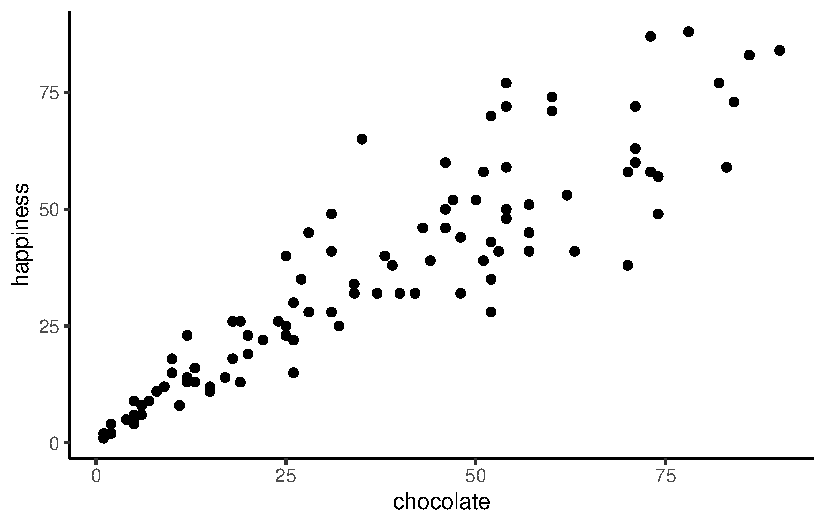
\includegraphics[width=0.75\textwidth,height=\textheight]{03-Correlation_files/figure-pdf/fig-3scatter1-1.pdf}

}

\caption{\label{fig-3scatter1}Imaginary data showing a positive
correlation between amount of chocolate and amount happiness}

\end{figure}

You might be wondering, why are there only 100 dots for the data. Didn't
we collect 100 measures for chocolate, and 100 measures for happiness,
shouldn't there be 200 dots? Nope. Each dot is for one subject, there
are 100 subjects, so there are 100 dots.

What do the dots mean? Each dot has two coordinates, an x-coordinate for
chocolate, and a y-coordinate for happiness. The first dot, all the way
on the bottom left is the first subject in the table, who had close to 0
chocolate and close to zero happiness. You can look at any dot, then
draw a straight line down to the x-axis: that will tell you how much
chocolate that subject has. You can draw a straight line left to the
y-axis: that will tell you how much happiness the subject has.

Now that we are looking at the scatter plot, we can see many things. The
dots are scattered around a bit aren't they, hence \textbf{scatter
plot}. Even when the dot's don't scatter, they're still called scatter
plots, perhaps because those pesky dots in real life have so much
scatter all the time. More important, the dots show a relationship
between chocolate supply and happiness. Happiness is lower for people
with smaller supplies of chocolate, and higher for people with larger
supplies of chocolate. It looks like the more chocolate you have the
happier you will be, and vice-versa. This kind of relationship is called
a \textbf{positive correlation}.

\hypertarget{positive-negative-and-no-correlation}{%
\subsection{Positive, Negative, and
No-Correlation}\label{positive-negative-and-no-correlation}}

Seeing as we are in the business of imagining data, let's imagine some
more. We've already imagined what data would look like if larger
chocolate supplies increase happiness. We'll show that again in a bit.
What do you imagine the scatter plot would look like if the relationship
was reversed, and larger chocolate supplies decreased happiness. Or,
what do you imagine the scatter plot would look like if there was no
relationship, and the amount of chocolate that you have doesn't do
anything to your happiness. We invite your imagination to look at
Figure~\ref{fig-3posnegrand}:

\begin{figure}

{\centering 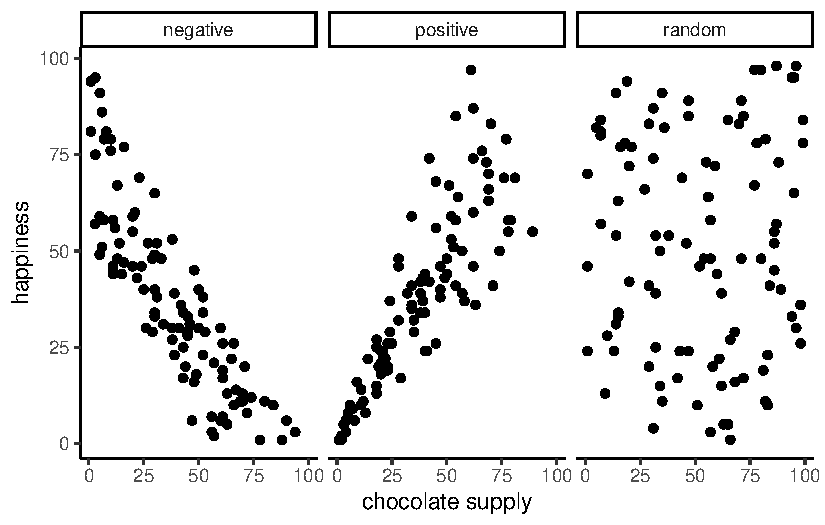
\includegraphics[width=0.75\textwidth,height=\textheight]{03-Correlation_files/figure-pdf/fig-3posnegrand-1.pdf}

}

\caption{\label{fig-3posnegrand}Three scatterplots showing negative,
positive, and zero correlation}

\end{figure}

The first panel shows a \textbf{negative correlation}. Happiness goes
down as chocolate supply increases. Negative correlation occurs when one
thing goes up and the other thing goes down; or, when more of X is less
of Y, and vice-versa. The second panel shows a \textbf{positive
correlation}. Happiness goes up as chocolate as chocolate supply
increases. Positive correlation occurs when both things go up together,
and go down together: more of X is more of Y, and vice-versa. The third
panel shows \textbf{no correlation}. Here, there doesn't appear to be
any obvious relationship between chocolate supply and happiness. The
dots are scattered all over the place, the truest of the scatter plots.

\begin{tcolorbox}[enhanced jigsaw, breakable, colback=white, coltitle=black, toptitle=1mm, rightrule=.15mm, title=\textcolor{quarto-callout-note-color}{\faInfo}\hspace{0.5em}{Note}, opacitybacktitle=0.6, opacityback=0, colframe=quarto-callout-note-color-frame, leftrule=.75mm, colbacktitle=quarto-callout-note-color!10!white, arc=.35mm, bottomtitle=1mm, titlerule=0mm, bottomrule=.15mm, toprule=.15mm, left=2mm]

We are wading into the idea that measures of two things can be related,
or correlated with one another. It is possible for the relationships to
be more complicated than just going up, or going down. For example, we
could have a relationship that where the dots go up for the first half
of X, and then go down for the second half.

\end{tcolorbox}

Zero correlation occurs when one thing is not related in any way to
another things: changes in X do not relate to any changes in Y, and
vice-versa.

\hypertarget{pearsons-r}{%
\section{Pearson's r}\label{pearsons-r}}

``So you've examined your scatter plots and now you might be wondering
how to quantify what you see. We've already covered how to generate
descriptive statistics for individual variables---think of single
measures like happiness levels or chocolate consumption, summarized
through means, variances, and so on. But what if you want to capture the
relationship between two such variables in a single descriptive
statistic? Is that even possible? Karl Pearson to the rescue.

\begin{tcolorbox}[enhanced jigsaw, breakable, colback=white, coltitle=black, toptitle=1mm, rightrule=.15mm, title=\textcolor{quarto-callout-note-color}{\faInfo}\hspace{0.5em}{Note}, opacitybacktitle=0.6, opacityback=0, colframe=quarto-callout-note-color-frame, leftrule=.75mm, colbacktitle=quarto-callout-note-color!10!white, arc=.35mm, bottomtitle=1mm, titlerule=0mm, bottomrule=.15mm, toprule=.15mm, left=2mm]

The stories about the invention of various statistics are very
interesting, you can read more about them in the book, ``The Lady
Tasting Tea'' (Salsburg 2001)

\end{tcolorbox}

There's a statistic for that, and Karl Pearson invented it. Everyone now
calls it, ``Pearson's \(r\)''. We will find out later that Karl Pearson
was a big-wig editor at Biometrika in the 1930s. He took a hating to
another big-wig statistician, Sir Ronald Fisher (who we learn about
later), and they had some statistics fights. Even in the stats world,
not everyone plays nice in the sandbox.

How does Pearson's \(r\) work? Let's look again at the first 10 subjects
in our fake experiment:

\begin{longtable}[]{@{}lll@{}}
\toprule\noalign{}
subject & chocolate & happiness \\
\midrule\noalign{}
\endhead
\bottomrule\noalign{}
\endlastfoot
1 & 1 & 1 \\
2 & 1 & 1 \\
3 & 2 & 2 \\
4 & 2 & 4 \\
5 & 3 & 4 \\
6 & 6 & 4 \\
7 & 6 & 4 \\
8 & 7 & 4 \\
9 & 5 & 6 \\
10 & 8 & 8 \\
Sums & 41 & 38 \\
Means & 4.1 & 3.8 \\
\end{longtable}

What could we do to these numbers to produce a single summary value that
represents the relationship between the chocolate supply and happiness?

\hypertarget{the-idea-of-co-variance}{%
\subsection{The idea of co-variance}\label{the-idea-of-co-variance}}

``Oh please no, don't use the word variance again''. Yes, we're doing
it, we're going to use the word variance again, and again, until it
starts making sense. Remember what variance means about some numbers. It
means the numbers have some change in them, they are not all the same,
some of them are big, some are small. We can see that there is variance
in chocolate supply across the 10 subjects. We can see that there is
variance in happiness across the 10 subjects. We also saw in the scatter
plot, that happiness increases as chocolate supply increases; which is a
positive relationship, a positive correlation. What does this have to do
with variance? Well, it means there is a relationship between the
variance in chocolate supply, and the variance in happiness levels. The
two measures vary together don't they? When we have two measures that
vary together, they are like a happy couple who share their variance.
This is what co-variance refers to, the idea that the pattern of varying
numbers in one measure is shared by the pattern of varying numbers in
another measure.

\textbf{Co-variance} is \textbf{very, very, very, very} important. I
suspect that the word co-variance is initially confusing, especially if
you are not yet fully comfortable with the meaning of variance for a
single measure. Nevertheless, we must proceed and use the idea of
co-variance over and over again to firmly implant it into your
statistical mind (we already said, but redundancy works, it's a thing).

\begin{quote}
Pro tip: Three-legged race is a metaphor for co-variance. Two people tie
one leg to each other, then try to walk. It works when they co-vary
their legs together (positive relationship). They can also co-vary in an
unhelpful way, when one person tries to move forward exactly when the
other person tries to move backward. This is still co-variance (negative
relationship). Funny random walking happens when there is no
co-variance. This means one person does whatever they want, and so does
the other person. There is a lot of variance, but the variance is shared
randomly, so it's just a bunch of legs moving around accomplishing
nothing.
\end{quote}

\begin{quote}
Pro tip \#2: Successfully playing paddy-cake occurs when two people
coordinate their actions so they have positively shared co-variance.
\end{quote}

\hypertarget{turning-the-numbers-into-a-measure-of-co-variance}{%
\section{Turning the numbers into a measure of
co-variance}\label{turning-the-numbers-into-a-measure-of-co-variance}}

``OK, so if you are saying that co-variance is just another word for
correlation or relationship between two measures, I'm good with that. I
suppose we would need some way to measure that.'' Correct, back to our
table\ldots notice anything new?

\begin{longtable}[]{@{}llll@{}}
\toprule\noalign{}
subject & chocolate & happiness & Chocolate\_X\_Happiness \\
\midrule\noalign{}
\endhead
\bottomrule\noalign{}
\endlastfoot
1 & 1 & 1 & 1 \\
2 & 1 & 1 & 1 \\
3 & 2 & 2 & 4 \\
4 & 2 & 4 & 8 \\
5 & 3 & 4 & 12 \\
6 & 6 & 4 & 24 \\
7 & 6 & 4 & 24 \\
8 & 7 & 4 & 28 \\
9 & 5 & 6 & 30 \\
10 & 8 & 8 & 64 \\
Sums & 41 & 38 & 196 \\
Means & 4.1 & 3.8 & 19.6 \\
\end{longtable}

We've added a new column called \texttt{Chocolate\_X\_Happiness}, which
translates to Chocolate scores multiplied by Happiness scores. Each row
in the new column, is the product, or multiplication of the chocolate
and happiness score for that row. Yes, but why would we do this?

Last chapter we took you back to Elementary school and had you think
about division. Now it's time to do the same thing with multiplication.
We assume you know how that works. One number times another, means
taking the first number, and adding it as many times as the second says
to do,

\(2*2= 2+2=4\)

\(2*6= 2+2+2+2+2+2 = 12\), or \(6+6=12\), same thing.

Yes, you know all that. But, can you bend multiplication to your will,
and make it do your bidding when need to solve a problem like
summarizing co-variance? Multiplication is the droid you are looking
for.

We know how to multiple numbers, and all we have to next is think about
the consequences of multiplying sets of numbers together. For example,
what happens when you multiply two small numbers together, compared to
multiplying two big numbers together? The first product should be
smaller than the second product right? How about things like multiplying
a small number by a big number? Those products should be in between
right?.

Then next step is to think about how the products of two measures sum
together, depending on how they line up. Let's look at another table:

\begin{longtable}[]{@{}lllllll@{}}
\toprule\noalign{}
scores & X & Y & A & B & XY & AB \\
\midrule\noalign{}
\endhead
\bottomrule\noalign{}
\endlastfoot
1 & 1 & 1 & 1 & 10 & 1 & 10 \\
2 & 2 & 2 & 2 & 9 & 4 & 18 \\
3 & 3 & 3 & 3 & 8 & 9 & 24 \\
4 & 4 & 4 & 4 & 7 & 16 & 28 \\
5 & 5 & 5 & 5 & 6 & 25 & 30 \\
6 & 6 & 6 & 6 & 5 & 36 & 30 \\
7 & 7 & 7 & 7 & 4 & 49 & 28 \\
8 & 8 & 8 & 8 & 3 & 64 & 24 \\
9 & 9 & 9 & 9 & 2 & 81 & 18 \\
10 & 10 & 10 & 10 & 1 & 100 & 10 \\
Sums & 55 & 55 & 55 & 55 & 385 & 220 \\
Means & 5.5 & 5.5 & 5.5 & 5.5 & 38.5 & 22 \\
\end{longtable}

Look at the \(X\) and \(Y\) column. The scores for \(X\) and \(Y\)
perfectly co-vary. When \(X\) is 1, \(Y\) is 1; when \(X\) is 2, \(Y\)
is 2, etc. They are perfectly aligned. The scores for \(A\) and \(B\)
also perfectly co-vary, just in the opposite manner. When \(A\) is 1,
\(B\) is 10; when \(A\) is 2, \(B\) is 9, etc. \(B\) is a reversed copy
of \(A\).

Now, look at the column \(XY\). These are the products we get when we
multiply the values of \(X\) across with the values of \(Y\). Also, look
at the column \(AB\). These are the products we get when we multiply the
values of A across with the values of B. So far so good.

Now, look at the \texttt{Sums} for the \(XY\) and \(AB\) columns. Not
the same. The sum of the \(XY\) products is 385, and the sum of the
\(AB\) products is 220. For this specific set of data, the numbers 385
and 220 are very important. They represent the biggest possible sum of
products (385), and the smallest possible sum of products (220). There
is no way of re-ordering the numbers 1 to 10, say for \(X\), and the
numbers 1 to 10 for \(Y\), that would ever produce larger or smaller
numbers. Don't believe me? Check this out:

\begin{figure}

{\centering 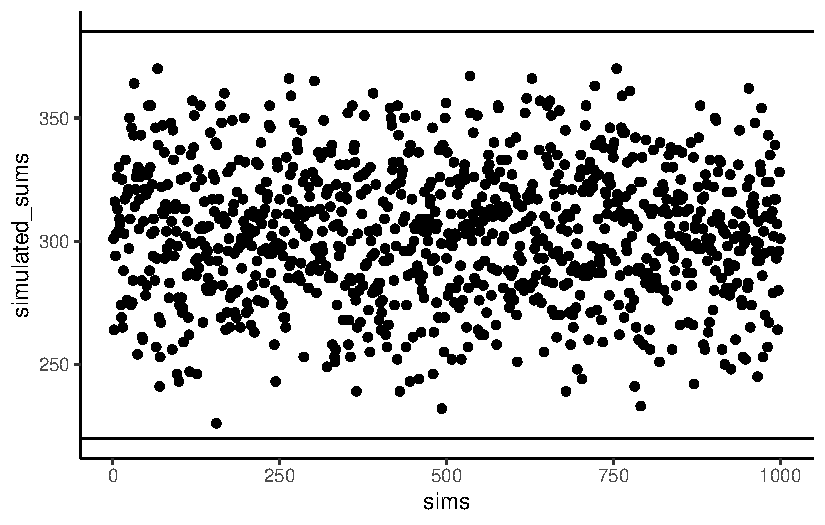
\includegraphics[width=0.75\textwidth,height=\textheight]{03-Correlation_files/figure-pdf/fig-3simsum-1.pdf}

}

\caption{\label{fig-3simsum}Simulated sums of products showing the kinds
of values than can be produced by randomly ordering the numbers in X and
Y.}

\end{figure}

Figure~\ref{fig-3simsum} shows 1000 computer simulations. I convinced my
computer to randomly order the numbers 1 to 10 for X, and randomly order
the numbers 1 to 10 for Y. Then, I multiplied X and Y, and added the
products together. I did this 1000 times. The dots show the sum of the
products for each simulation. The two black lines show the maximum
possible sum (385), and the minimum possible sum (220), for this set of
numbers. Notice, how all of the dots are in between the maximum and
minimum possible values. Told you so.

``OK fine, you told me so\ldots So what, who cares?''. We've been
looking for a way to summarize the co-variance between two measures
right? Well, for these numbers, we have found one, haven't we. It's the
sum of the products. We know that when the sum of the products is 385,
we have found a perfect, positive correlation. We know, that when the
sum of the products is 220, we have found a perfect negative
correlation. What about the numbers in between. What could we conclude
about the correlation if we found the sum of the products to be 350.
Well, it's going to be positive, because it's close to 385, and that's
perfectly positive. If the sum of the products was 240, that's going to
be negative, because it's close to the perfectly negatively correlating
220. What about no correlation? Well, that's going to be in the middle
between 220 and 385 right.

We have just come up with a data-specific summary measure for the
correlation between the numbers 1 to 10 in X, and the numbers 1 to 10 in
Y, it's the sum of the products. We know the maximum (385) and minimum
values (220), so we can now interpret any product sum for this kind of
data with respect to that scale.

\begin{quote}
Pro tip: When the correlation between two measures increases in the
positive direction, the sum of their products increases to its maximum
possible value. This is because the bigger numbers in X will tend to
line up with the bigger numbers in Y, creating the biggest possible sum
of products. When the correlation between two measures increases in the
negative direction, the sum of their products decreases to its minimum
possible value. This is because the bigger numbers in X will tend to
line up with the smaller numbers in Y, creating the smallest possible
sum of products. When there is no correlation, the big numbers in X will
be randomly lined up with the big and small numbers in Y, making the sum
of the products, somewhere in the middle.
\end{quote}

\hypertarget{co-variance-the-measure}{%
\subsection{Co-variance, the measure}\label{co-variance-the-measure}}

We took some time to see what happens when you multiply sets of numbers
together. We found that \(big*big = bigger\) and
\(small*small=\text{still small}\), and
\(big*small=\text{in the middle}\). The purpose of this was to give you
some conceptual idea of how the co-variance between two measures is
reflected in the sum of their products. We did something very
straightforward. We just multiplied X with Y, and looked at how the
product sums get big and small, as X and Y co-vary in different ways.

Now, we can get a little bit more formal. In statistics,
\textbf{co-variance} is not just the straight multiplication of values
in X and Y. Instead, it's the multiplication of the deviations in X from
the mean of X, and the deviation in Y from the mean of Y. Remember those
difference scores from the mean we talked about last chapter? They're
coming back to haunt you know, but in a good way like Casper the
friendly ghost.

Let's see what this look like in a table:

\begin{longtable}[]{@{}llllll@{}}
\toprule\noalign{}
subject & chocolate & happiness & C\_d & H\_d & Cd\_x\_Hd \\
\midrule\noalign{}
\endhead
\bottomrule\noalign{}
\endlastfoot
1 & 1 & 1 & -3.1 & -2.8 & 8.68 \\
2 & 1 & 1 & -3.1 & -2.8 & 8.68 \\
3 & 2 & 2 & -2.1 & -1.8 & 3.78 \\
4 & 2 & 4 & -2.1 & 0.2 & -0.42 \\
5 & 3 & 4 & -1.1 & 0.2 & -0.22 \\
6 & 6 & 4 & 1.9 & 0.2 & 0.38 \\
7 & 6 & 4 & 1.9 & 0.2 & 0.38 \\
8 & 7 & 4 & 2.9 & 0.2 & 0.58 \\
9 & 5 & 6 & 0.9 & 2.2 & 1.98 \\
10 & 8 & 8 & 3.9 & 4.2 & 16.38 \\
Sums & 41 & 38 & 0 & 0 & 40 \\
Means & 4.1 & 3.8 & 0 & 0 & 4.02 \\
\end{longtable}

We have computed the deviations from the mean for the chocolate scores
(column \texttt{C\_d}), and the deviations from the mean for the
happiness scores (column \texttt{H\_d}). Then, we multiplied them
together (last column). Finally, you can see the mean of the products
listed in the bottom right corner of the table, the official \textbf{the
covariance}.

The formula for the co-variance is:

\(cov(X,Y) = \frac{\sum_{i}^{n}(x_{i}-\bar{X})(y_{i}-\bar{Y})}{N}\)

OK, so now we have a formal single number to calculate the relationship
between two variables. This is great, it's what we've been looking for.
However, there is a problem. Remember when we learned how to compute
just the plain old \textbf{variance}. We looked at that number, and we
didn't know what to make of it. It was squared, it wasn't in the same
scale as the original data. So, we square rooted the \textbf{variance}
to produce the \textbf{standard deviation}, which gave us a more
interpretable number in the range of our data. The \textbf{co-variance}
has a similar problem. When you calculate the co-variance as we just
did, we don't know immediately know its scale. Is a 3 big? is a 6 big?
is a 100 big? How big or small is this thing?

From our prelude discussion on the idea of co-variance, we learned the
sum of products between two measures ranges between a maximum and
minimum value. The same is true of the co-variance. For a given set of
data, there is a maximum possible positive value for the co-variance
(which occurs when there is perfect positive correlation). And, there is
a minimum possible negative value for the co-variance (which occurs when
there is a perfect negative correlation). When there is zero
co-variation, guess what happens. Zeroes. So, at the very least, when we
look at a co-variation statistic, we can see what direction it points,
positive or negative. But, we don't know how big or small it is compared
to the maximum or minimum possible value, so we don't know the relative
size, which means we can't say how strong the correlation is. What to
do?

\hypertarget{pearsons-r-we-there-yet}{%
\subsection{Pearson's r we there yet}\label{pearsons-r-we-there-yet}}

Yes, we are here now. Wouldn't it be nice if we could force our measure
of co-variation to be between -1 and +1?

-1 would be the minimum possible value for a perfect negative
correlation. +1 would be the maximum possible value for a perfect
positive correlation. 0 would mean no correlation. Everything in between
0 and -1 would be increasingly large negative correlations. Everything
between 0 and +1 would be increasingly large positive correlations. It
would be a fantastic, sensible, easy to interpret system. If only we
could force the co-variation number to be between -1 and 1. Fortunately,
for us, this episode is brought to you by Pearson's \(r\), which does
precisely this wonderful thing.

Let's take a look at a formula for Pearson's \(r\):

\(r = \frac{cov(X,Y)}{\sigma_{X}\sigma_{Y}} = \frac{cov(X,Y)}{SD_{X}SD_{Y}}\)

We see the symbol \(\sigma\) here, that's more Greek for you. \(\sigma\)
is often used as a symbol for the standard deviation (SD). If we read
out the formula in English, we see that r is the co-variance of X and Y,
divided by the product of the standard deviation of X and the standard
deviation of Y. Why are we dividing the co-variance by the product of
the standard deviations. This operation has the effect of
\textbf{normalizing} the co-variance into the range -1 to 1.

\begin{tcolorbox}[enhanced jigsaw, breakable, colback=white, coltitle=black, toptitle=1mm, rightrule=.15mm, title=\textcolor{quarto-callout-note-color}{\faInfo}\hspace{0.5em}{Note}, opacitybacktitle=0.6, opacityback=0, colframe=quarto-callout-note-color-frame, leftrule=.75mm, colbacktitle=quarto-callout-note-color!10!white, arc=.35mm, bottomtitle=1mm, titlerule=0mm, bottomrule=.15mm, toprule=.15mm, left=2mm]

But, we will fill this part in as soon as we can\ldots promissory note
to explain the magic. FYI, it's not magic. Brief explanation here is
that dividing each measure by its standard deviation ensures that the
values in each measure are in the same range as one another.

\end{tcolorbox}

For now, we will call this mathematical magic. It works, but we don't
have space to tell you why it works right now.

It's worth saying that there are loads of different formulas for
computing Pearson's \(r\). You can find them by Googling them. We will
probably include more of them here, when we get around to it. However,
they all give you the same answer. And, they are all not as pretty as
each other. Some of them might even look scary. In other statistics
textbook you will often find formulas that are easier to use for
calculation purposes. For example, if you only had a pen and paper, you
might use one or another formula because it helps you compute the answer
faster by hand. To be honest, we are not very interested in teaching you
how to plug numbers into formulas. We give one lesson on that here: Put
the numbers into the letters, then compute the answer. Sorry to be
snarky. Nowadays you have a computer that you should use for this kind
of stuff. So, we are more interested in teaching you what the
calculations mean, rather than how to do them. Of course, every week we
are showing you how to do the calculations in lab with computers,
because that is important too.

Does Pearson's \(r\) really stay between -1 and 1 no matter what? It's
true, take a look at the following simulation. Here I randomly ordered
the numbers 1 to 10 for an X measure, and did the same for a Y measure.
Then, I computed Pearson's \(r\), and repeated this process 1000 times.
As you can see from Figure~\ref{fig-3onethousandr} all of the dots are
between -1 and 1. Neat huh.

\begin{figure}

{\centering 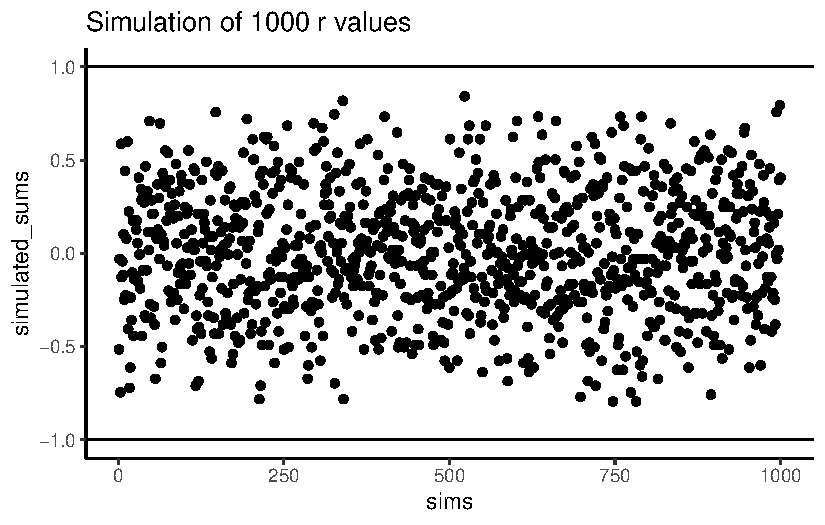
\includegraphics[width=0.75\textwidth,height=\textheight]{03-Correlation_files/figure-pdf/fig-3onethousandr-1.pdf}

}

\caption{\label{fig-3onethousandr}A simulation of of correlations. Each
dot represents the r-value for the correlation between an X and Y
variable that each contain the numbers 1 to 10 in random orders. The
figure ilustrates that many r-values can be obtained by this random
process}

\end{figure}

\hypertarget{examples-with-data}{%
\section{Examples with Data}\label{examples-with-data}}

In the lab for correlation you will be shown how to compute correlations
in real data-sets using software. To give you a brief preview, let's
look at some data from the \href{http://worldhappiness.report}{world
happiness report} (2018).

This report measured various attitudes across people from different
countries. For example, one question asked about how much freedom people
thought they had to make life choices. Another question asked how
confident people were in their national government.
\textbf{?@fig-3hrsdata} is a scatterplot showing the relationship
between these two measures. Each dot represents means for different
countries.

\begin{figure}

{\centering 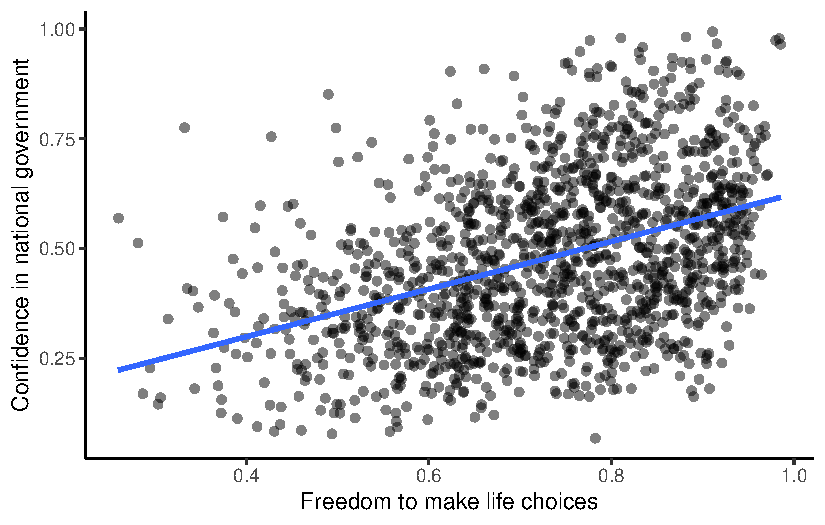
\includegraphics[width=0.75\textwidth,height=\textheight]{03-Correlation_files/figure-pdf/fig-3hsrdata-1.pdf}

}

\caption{\label{fig-3hsrdata}Relationship between freedom to make life
choices and confidence in national government. Data from the world
happiness report for 2018}

\end{figure}

We put a blue line on the scatterplot to summarize the positive
relationship. It appears that as ``freedom to make life choices goes
up'', so to does confidence in national government. It's a positive
correlation.

The actual correlation, as measured by Pearson's \(r\) is:

\begin{verbatim}
#> [1] 0.4080963
\end{verbatim}

You will do a lot more of this kind of thing in the lab. Looking at the
graph you might start to wonder: Does freedom to make life choices cause
changes how confident people are in their national government? Our does
it work the other way? Does being confident in your national government
give you a greater sense of freedom to make life choices? Or, is this
just a random relationship that doesn't mean anything? All good
questions. These data do not provide the answers, they just suggest a
possible relationship.

\hypertarget{regression-a-mini-intro}{%
\section{Regression: A mini intro}\label{regression-a-mini-intro}}

We're going to spend the next little bit adding one more thing to our
understanding of correlation. It's called \textbf{linear regression}. It
sounds scary, and it really is. You'll find out much later in your
Statistics education that everything we will be soon be talking about
can be thought of as a special case of regression. But, we don't want to
scare you off, so right now we just introduce the basic concepts.

First, let's look at a linear regression. This way we can see what we're
trying to learn about. Figure~\ref{fig-3regression} shows the same
scatter plots as before with something new: lines!

\begin{figure}

{\centering 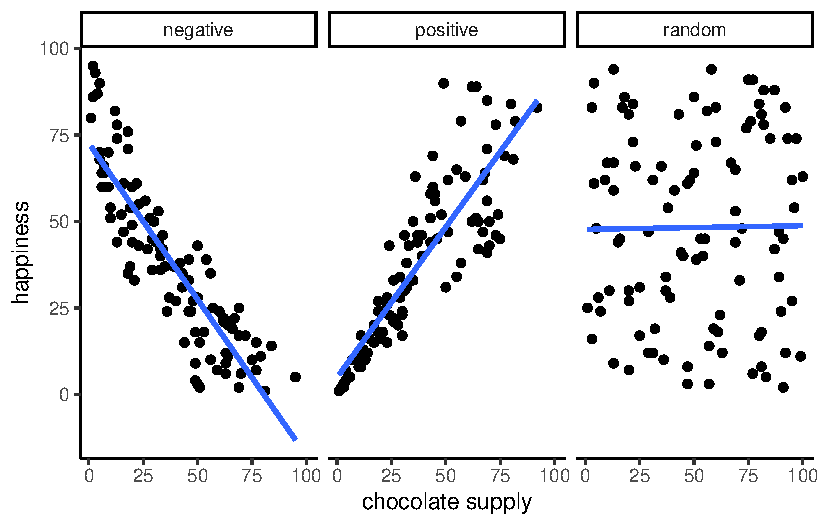
\includegraphics[width=0.75\textwidth,height=\textheight]{03-Correlation_files/figure-pdf/fig-3regression-1.pdf}

}

\caption{\label{fig-3regression}Three scatterplots showing negative,
positive, and a random correlation (where the r-value is expected to be
0), along with the best fit regression line}

\end{figure}

\hypertarget{the-best-fit-line}{%
\subsection{The best fit line}\label{the-best-fit-line}}

Notice anything about these blue lines? Hopefully you can see, at least
for the first two panels, that they go straight through the data, just
like a kebab skewer. We call these lines \textbf{best fit} lines,
because according to our definition (soon we promise) there are no other
lines that you could draw that would do a better job of going straight
throw the data.

One big idea here is that we are using the line as a kind of mean to
describe the relationship between the two variables. When we only have
one variable, that variable exists on a single dimension, it's 1D. So,
it is appropriate that we only have one number, like the mean, to
describe it's central tendency. When we have two variables, and plot
them together, we now have a two-dimensional space. So, for two
dimensions we could use a bigger thing that is 2d, like a line, to
summarize the central tendency of the relationship between the two
variables.

What do we want out of our line? Well, if you had a pencil, and a
printout of the data, you could draw all sorts of straight lines any way
you wanted. Your lines wouldn't even have to go through the data, or
they could slant through the data with all sorts of angles. Would all of
those lines be very good a describing the general pattern of the dots?
Most of them would not. The best lines would go through the data
following the general shape of the dots. Of the best lines, however,
which one is the best? How can we find out, and what do we mean by that?
In short, the best fit line is the one that has the least error.

\begin{tcolorbox}[enhanced jigsaw, breakable, colback=white, coltitle=black, toptitle=1mm, rightrule=.15mm, title=\textcolor{quarto-callout-note-color}{\faInfo}\hspace{0.5em}{Note}, opacitybacktitle=0.6, opacityback=0, colframe=quarto-callout-note-color-frame, leftrule=.75mm, colbacktitle=quarto-callout-note-color!10!white, arc=.35mm, bottomtitle=1mm, titlerule=0mm, bottomrule=.15mm, toprule=.15mm, left=2mm]

R code for plotting residuals thanks to Simon Jackson's blog post:
\url{https://drsimonj.svbtle.com/visualising-residuals}

\end{tcolorbox}

Check out this next plot, it shows a line through some dots. But, it
also shows some teeny tiny lines. These lines drop down from each dot,
and they land on the line. Each of these little lines is called a
\textbf{residual}. They show you how far off the line is for different
dots. It's measure of error, it shows us just how wrong the line is.
After all, it's pretty obvious that not all of the dots are on the line.
This means the line does not actually represent all of the dots. The
line is wrong. But, the best fit line is the least wrong of all the
wrong lines.

\begin{figure}

{\centering 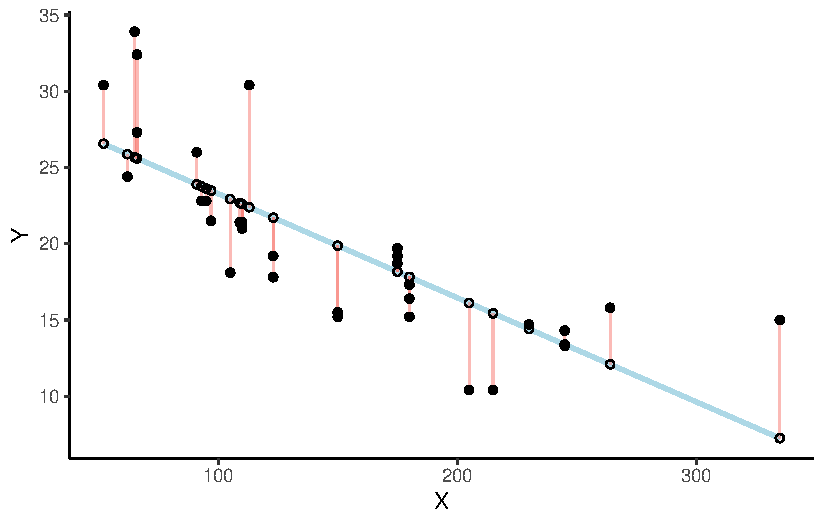
\includegraphics[width=0.75\textwidth,height=\textheight]{03-Correlation_files/figure-pdf/fig-3regressionResiduals-1.pdf}

}

\caption{\label{fig-3regressionResiduals}Black dots represent data
points. The blue line is the best fit regression line. The white dots
are repesent the predicted location of each black dot. The red lines
show the error between each black dot and the regression line. The blue
line is the best fit line because it minimizes the error shown by the
red lines.}

\end{figure}

There's a lot going on in Figure~\ref{fig-3regressionResiduals}. First,
we are looking at a scatter plot of two variables, an X and Y variable.
Each of the black dots are the actual values from these variables. You
can see there is a negative correlation here, as X increases, Y tends to
decrease. We drew a regression line through the data, that's the blue
line. There's these little white dots too. This is where the line thinks
the black dots should be. The red lines are the important residuals
we've been talking about. Each black dot has a red line that drops
straight down, or straight up from the location of the black dot, and
lands directly on the line. We can already see that many of the dots are
not on the line, so we already know the line is ``off'' by some amount
for each dot. The red line just makes it easier to see exactly how off
the line is.

The important thing that is happening here, is that the the blue line is
drawn is such a way, that it minimizes the total length of the red
lines. For example, if we wanted to know how wrong this line was, we
could simply gather up all the red lines, measure how long they are, and
then add all the wrongness together. This would give us the total amount
of wrongness. We usually call this the error. In fact, we've already
talked about this idea before when we discussed standard deviation. What
we will actually be doing with the red lines, is computing the sum of
the squared deviations from the line. That sum is the total amount of
error. Now, this blue line here minimizes the sum of the squared
deviations. Any other line would produce a larger total error.

\textbf{?@fig-3regressionGIF} is an animation to see this in action. The
animations compares the best fit line in blue, to some other possible
lines in black. The black line moves up and down. The red lines show the
error between the black line and the data points. As the black line
moves toward the best fit line, the total error, depicted visually by
the grey area shrinks to it's minimum value. The total error expands as
the black line moves away from the best fit line.

Whenever the black line does not overlap with the blue line, it is worse
than the best fit line. The blue regression line is like Goldilocks,
it's just right, and it's in the middle.

Figure~\ref{fig-3minimizeSS} shows how the sum of squared deviations
(the sum of the squared lengths of the red lines) behaves as we move the
line up and down. What's going on here is that we are computing a
measure of the total error as the black line moves through the best fit
line. This represents the sum of the squared deviations. In other words,
we square the length of each red line from the above animation, then we
add up all of the squared red lines, and get the total error (the total
sum of the squared deviations). The graph below shows what the total
error looks like as the black line approaches then moves away from the
best fit line. Notice, the dots in this graph start high on the left
side, then they swoop down to a minimum at the bottom middle of the
graph. When they reach their minimum point, we have found a line that
minimizes the total error. This is the best fit regression line.

\begin{figure}

{\centering 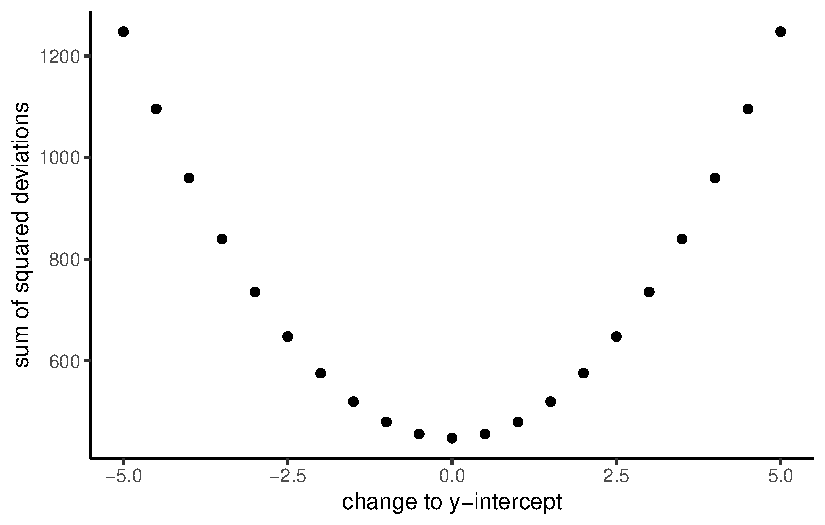
\includegraphics[width=0.75\textwidth,height=\textheight]{03-Correlation_files/figure-pdf/fig-3minimizeSS-1.pdf}

}

\caption{\label{fig-3minimizeSS}A plot of the sum of the squared
deviations for different lines moving up and down, through the best fit
line. The best fit line occurs at the position that minimizes the sum of
the sqaured deviations.}

\end{figure}

OK, so we haven't talked about the y-intercept yet. But, what this graph
shows us is how the total error behaves as we move the line up and down.
The y-intercept here is the thing we change that makes our line move up
and down. As you can see the dots go up when we move the line down from
0 to -5, and the dots go up when we move the line up from 0 to +5. The
best line, that minimizes the error occurs right in the middle, when we
don't move the blue regression line at all.

\hypertarget{lines}{%
\subsection{Lines}\label{lines}}

OK, fine you say. So, there is one magic line that will go through the
middle of the scatter plot and minimize the sum of the squared
deviations. How do I find this magic line? We'll show you. But, to be
completely honest, you'll almost never do it the way we'll show you
here. Instead, it's much easier to use software and make your computer
do it for. You'll learn how to that in the labs.

Before we show you how to find the regression line, it's worth
refreshing your memory about how lines work, especially in 2 dimensions.
Remember this?

\(y = ax + b\), or also \(y = mx + b\) (sometimes a or m is used for the
slope)

This is the formula for a line. Another way of writing it is:

\(y = slope * x + \text{y-intercept}\)

The slope is the slant of the line, and the y-intercept is where the
line crosses the y-axis. Let's look at the lines in
Figure~\ref{fig-3twolines}.

\begin{figure}

{\centering 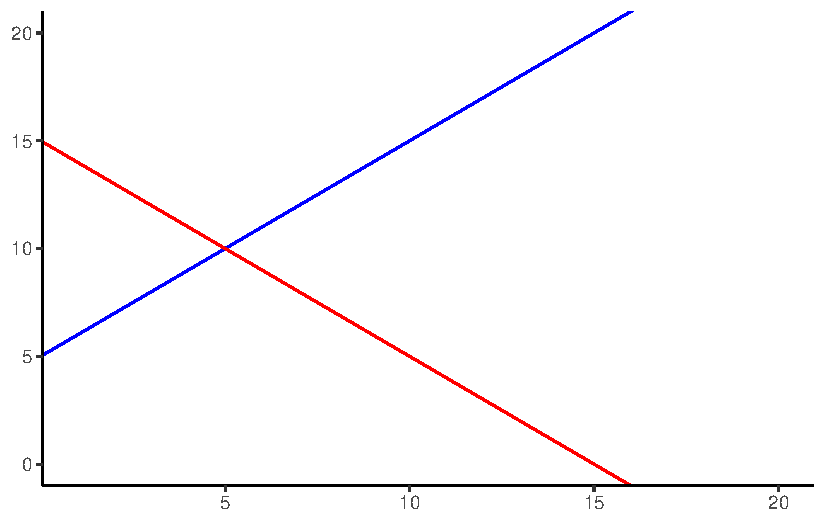
\includegraphics[width=0.5\textwidth,height=\textheight]{03-Correlation_files/figure-pdf/fig-3twolines-1.pdf}

}

\caption{\label{fig-3twolines}Two different lines with different
y-intercepts (where the line crosses the y-axis), and different slopes.
A positive slope makes the line go up from left to right. A negative
slope makes the line go down from left to right.}

\end{figure}

The formula for the blue line is \(y = 1*x + 5\). Let's talk about that.
When x = 0, where is the blue line on the y-axis? It's at five. That
happens because 1 times 0 is 0, and then we just have the five left
over. How about when x = 5? In that case y =10. You just need the plug
in the numbers to the formula, like this:

\(y = 1*x + 5\) \(y = 1*5 + 5 = 5+5 =10\)

The point of the formula is to tell you where y will be, for any number
of x. The slope of the line tells you whether the line is going to go up
or down, as you move from the left to the right. The blue line has a
positive slope of one, so it goes up as x goes up. How much does it go
up? It goes up by one for everyone one of x! If we made the slope a 2,
it would be much steeper, and go up faster. The red line has a negative
slope, so it slants down. This means \(y\) goes down, as \(x\) goes up.
When there is no slant, and we want to make a perfectly flat line, we
set the slope to 0. This means that y doesn't go anywhere as x gets
bigger and smaller.

That's lines.

\hypertarget{computing-the-best-fit-line}{%
\subsection{Computing the best fit
line}\label{computing-the-best-fit-line}}

If you have a scatter plot showing the locations of scores from two
variables, the real question is how can you find the slope and the
y-intercept for the best fit line? What are you going to do? Draw
millions of lines, add up the residuals, and then see which one was
best? That would take forever. Fortunately, there are computers, and
when you don't have one around, there's also some handy formulas.

\begin{tcolorbox}[enhanced jigsaw, breakable, colback=white, coltitle=black, toptitle=1mm, rightrule=.15mm, title=\textcolor{quarto-callout-note-color}{\faInfo}\hspace{0.5em}{Note}, opacitybacktitle=0.6, opacityback=0, colframe=quarto-callout-note-color-frame, leftrule=.75mm, colbacktitle=quarto-callout-note-color!10!white, arc=.35mm, bottomtitle=1mm, titlerule=0mm, bottomrule=.15mm, toprule=.15mm, left=2mm]

It's worth pointing out just how much computers have changed everything.
Before computers everyone had to do these calculations by hand, such a
chore! Aside from the deeper mathematical ideas in the formulas, many of
them were made for convenience, to speed up hand calculations, because
there were no computers. Now that we have computers, the hand
calculations are often just an exercise in algebra. Perhaps they build
character. You decide.

\end{tcolorbox}

We'll show you the formulas. And, work through one example by hand. It's
the worst, we know. By the way, you should feel sorry for me as I do
this entire thing by hand for you.

Here are two formulas we can use to calculate the slope and the
intercept, straight from the data. We won't go into why these formulas
do what they do. These ones are for ``easy'' calculation.

\(intercept = b = \frac{\sum{y}\sum{x^2}-\sum{x}\sum{xy}}{n\sum{x^2}-(\sum{x})^2}\)

\(slope = m = \frac{n\sum{xy}-\sum{x}\sum{y}}{n\sum{x^2}-(\sum{x})^2}\)

In these formulas, the \(x\) and the \(y\) refer to the individual
scores. Here's a table showing you how everything fits together.

\begin{longtable}[]{@{}llllll@{}}
\toprule\noalign{}
scores & x & y & x\_squared & y\_squared & xy \\
\midrule\noalign{}
\endhead
\bottomrule\noalign{}
\endlastfoot
1 & 1 & 2 & 1 & 4 & 2 \\
2 & 4 & 5 & 16 & 25 & 20 \\
3 & 3 & 1 & 9 & 1 & 3 \\
4 & 6 & 8 & 36 & 64 & 48 \\
5 & 5 & 6 & 25 & 36 & 30 \\
6 & 7 & 8 & 49 & 64 & 56 \\
7 & 8 & 9 & 64 & 81 & 72 \\
Sums & 34 & 39 & 200 & 275 & 231 \\
\end{longtable}

We see 7 sets of scores for the x and y variable. We calculated \(x^2\)
by squaring each value of x, and putting it in a column. We calculated
\(y^2\) by squaring each value of y, and putting it in a column. Then we
calculated \(xy\), by multiplying each \(x\) score with each \(y\)
score, and put that in a column. Then we added all the columns up, and
put the sums at the bottom. These are all the number we need for the
formulas to find the best fit line. Here's what the formulas look like
when we put numbers in them:

\(intercept = b = \frac{\sum{y}\sum{x^2}-\sum{x}\sum{xy}}{n\sum{x^2}-(\sum{x})^2} = \frac{39 * 200 - 34*231}{7*200-34^2} = -.221\)

\(slope = m = \frac{n\sum{xy}-\sum{x}\sum{y}}{n\sum{x^2}-(\sum{x})^2} = \frac{7*231-34*39}{7*275-34^2} = 1.19\)

Great, now we can check our work, let's plot the scores in a scatter
plot and draw a line through it with slope = 1.19, and a y-intercept of
-.221. As shown in Figure~\ref{fig-3corwithLine}, the line should go
through the middle of the dots.

\begin{figure}

{\centering 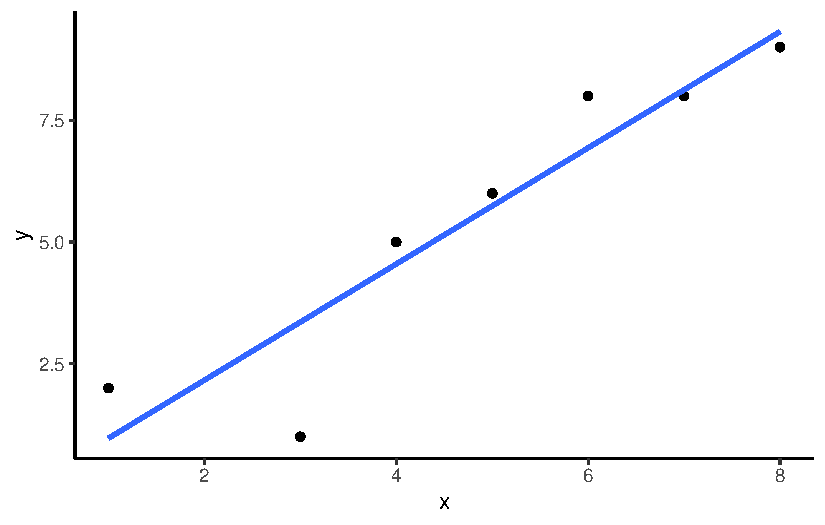
\includegraphics[width=0.75\textwidth,height=\textheight]{03-Correlation_files/figure-pdf/fig-3corwithLine-1.pdf}

}

\caption{\label{fig-3corwithLine}An example regression line with
confidence bands going through a few data points in a scatterplot}

\end{figure}

\hypertarget{interpreting-correlations}{%
\section{Interpreting Correlations}\label{interpreting-correlations}}

What does the presence or the absence of a correlation between two
measures mean? How should correlations be interpreted? What kind of
inferences can be drawn from correlations? These are all very good
questions. A first piece of advice is to use caution when interpreting
correlations. Here's why.

\hypertarget{correlation-does-not-equal-causation}{%
\subsection{Correlation does not equal
causation}\label{correlation-does-not-equal-causation}}

Perhaps you have heard that correlation does not equal causation. Why
not? There are lots of reasons why not. However, before listing some of
the reasons let's start with a case where we would expect a causal
connection between two measurements. Consider, buying a snake plant for
your home. Snake plants are supposed to be easy to take care of because
you can mostly ignore them.

Like most plants, snake plants need some water to stay alive. However,
they also need just the right amount of water. Imagine an experiment
where 1000 snake plants were grown in a house. Each snake plant is given
a different amount of water per day, from zero teaspoons of water per
day to 1000 teaspoons of water per day. We will assume that water is
part of the causal process that allows snake plants to grow. The amount
of water given to each snake plant per day can also be one of our
measures. Imagine further that every week the experimenter measures
snake plant growth, which will be the second measurement. Now, can you
imagine for yourself what a scatter plot of weekly snake plant growth by
tablespoons of water would look like?

\hypertarget{even-when-there-is-causation-there-might-not-be-obvious-correlation}{%
\subsubsection{Even when there is causation, there might not be obvious
correlation}\label{even-when-there-is-causation-there-might-not-be-obvious-correlation}}

The first plant given no water at all would have a very hard time and
eventually die. It should have the least amount of weekly growth. How
about the plants given only a few teaspoons of water per day. This could
be just enough water to keep the plants alive, so they will grow a
little bit but not a lot. If you are imagining a scatter plot, with each
dot being a snake plant, then you should imagine some dots starting in
the bottom left hand corner (no water \& no plant growth), moving up and
to the right (a bit of water, and a bit of growth). As we look at snake
plants getting more and more water, we should see more and more plant
growth, right? ``Sure, but only up to a point''. Correct, there should
be a trend for a positive correlation with increasing plant growth as
amount of water per day increases. But, what happens when you give snake
plants too much water? From personal experience, they die. So, at some
point, the dots in the scatter plot will start moving back down again.
Snake plants that get way too much water will not grow very well.

The imaginary scatter plot you should be envisioning could have an
upside U shape. Going from left to right, the dot's go up, they reach a
maximum, then they go down again reaching a minimum. Computing Pearson's
\(r\) for data like this can give you \(r\) values close to zero. The
scatter plot could look something like Figure~\ref{fig-3snakeplant}.

\begin{figure}

{\centering 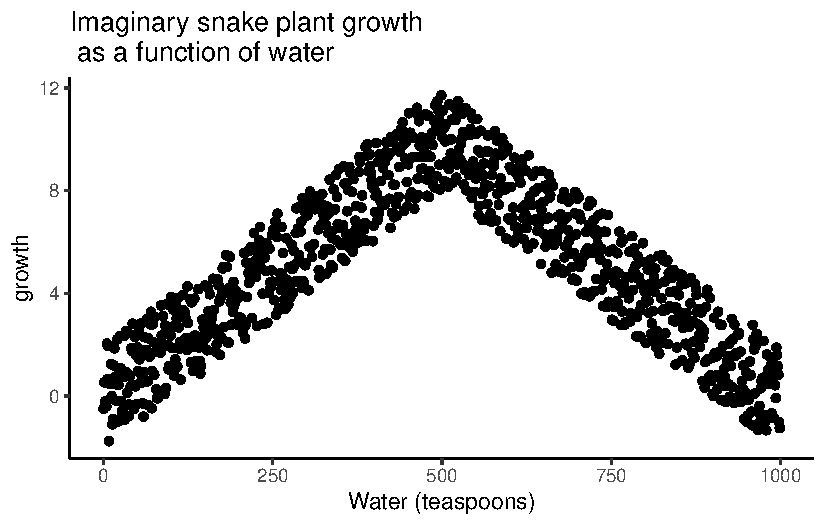
\includegraphics[width=0.75\textwidth,height=\textheight]{03-Correlation_files/figure-pdf/fig-3snakeplant-1.pdf}

}

\caption{\label{fig-3snakeplant}Illustration of a possible relationship
between amount of water and snake plant growth. Growth goes up with
water, but eventually goes back down as too much water makes snake
plants die.}

\end{figure}

Granted this looks more like an inverted V, than an inverted U, but you
get the picture right? There is clearly a relationship between watering
and snake plant growth. But, the correlation isn't in one direction. As
a result, when we compute the correlation in terms of Pearson's r, we
get a value suggesting no relationship.

\begin{verbatim}
#> [1] -0.001845471
\end{verbatim}

What this really means is there is no linear relationship that can be
described by a single straight line. When we need lines or curves going
in more than one direction, we have a nonlinear relationship.

This example illustrates some conundrums in interpreting correlations.
We already know that water is needed for plants to grow, so we are
rightly expecting there to be a relationship between our measure of
amount of water and plant growth. If we look at the first half of the
data we see a positive correlation, if we look at the last half of the
data we see a negative correlation, and if we look at all of the data we
see no correlation. Yikes. So, even when there is a causal connection
between two measures, we won't necessarily obtain clear evidence of the
connection just by computing a correlation coefficient.

\begin{quote}
Pro Tip: This is one reason why plotting your data is so important. If
you see an upside U shape pattern, then a correlation analysis is
probably not the best analysis for your data.
\end{quote}

\hypertarget{confounding-variable-or-third-variable-problem}{%
\subsubsection{Confounding variable, or Third variable
problem}\label{confounding-variable-or-third-variable-problem}}

Anybody can correlate any two things that can be quantified and
measured. For example, we could find a hundred people, ask them all
sorts of questions like:

\begin{enumerate}
\def\labelenumi{\arabic{enumi}.}
\tightlist
\item
  how happy are you
\item
  how old are you
\item
  how tall are you
\item
  how much money do you make per year
\item
  how long are your eyelashes
\item
  how many books have you read in your life
\item
  how loud is your inner voice
\end{enumerate}

Let's say we found a positive correlation between yearly salary and
happiness. Note, we could have just as easily computed the same
correlation between happiness and yearly salary. If we found a
correlation, would you be willing to infer that yearly salary causes
happiness? Perhaps it does play a small part. But, something like
happiness probably has a lot of contributing causes. Money could
directly cause some people to be happy. But, more likely, money buys
people access to all sorts of things, and some of those things might
contribute happiness. These ``other'' things are called \textbf{third}
variables. For example, perhaps people living in nicer places in more
expensive houses are more happy than people in worse places in cheaper
houses. In this scenario, money isn't causing happiness, it's the places
and houses that money buys. But, even is this were true, people can
still be more or less happy in lots of different situations.

The lesson here is that a correlation can occur between two measures
because of a third variable that is not directly measured. So, just
because we find a correlation, does not mean we can conclude anything
about a causal connection between two measurements.

\hypertarget{correlation-and-random-chance}{%
\subsection{Correlation and Random
chance}\label{correlation-and-random-chance}}

Another very important aspect of correlations is the fact that they can
be produced by random chance. This means that you can find a positive or
negative correlation between two measures, even when they have
absolutely nothing to do with one another. You might have hoped to find
zero correlation when two measures are totally unrelated to each other.
Although this certainly happens, unrelated measures can accidentally
produce \textbf{spurious} correlations, just by chance alone.

Let's demonstrate how correlations can occur by chance when there is no
causal connection between two measures. Imagine two participants. One is
at the North pole with a lottery machine full of balls with numbers from
1 to 10. The other is at the south pole with a different lottery machine
full of balls with numbers from 1 to 10. There are an endless supply of
balls in the machine, so every number could be picked for any ball. Each
participant randomly chooses 10 balls, then records the number on the
ball. In this situation we will assume that there is no possible way
that balls chosen by the first participant could causally influence the
balls chosen by the second participant. They are on the other side of
the world. We should assume that the balls will be chosen by chance
alone.

Here is what the numbers on each ball could look like for each
participant:

\begin{longtable}[]{@{}rrr@{}}
\toprule\noalign{}
Ball & North\_pole & South\_pole \\
\midrule\noalign{}
\endhead
\bottomrule\noalign{}
\endlastfoot
1 & 3 & 5 \\
2 & 6 & 8 \\
3 & 2 & 6 \\
4 & 3 & 5 \\
5 & 7 & 9 \\
6 & 2 & 7 \\
7 & 1 & 9 \\
8 & 6 & 10 \\
9 & 8 & 8 \\
10 & 3 & 6 \\
\end{longtable}

In this one case, if we computed Pearson's \(r\), we would find that
\(r =\) 0.4850211. But, we already know that this value does not tell us
anything about the relationship between the balls chosen in the north
and south pole. We know that relationship should be completely random,
because that is how we set up the game.

The better question here is to ask what can random chance do? For
example, if we ran our game over and over again thousands of times, each
time choosing new balls, and each time computing the correlation, what
would we find?First, we will find fluctuation. The r value will
sometimes be positive, sometimes be negative, sometimes be big and
sometimes be small. Second, we will see what the fluctuation looks like.
This will give us a window into the kinds of correlations that chance
alone can produce. Let's see what happens.

\hypertarget{monte-carlo-simulation-of-random-correlations}{%
\subsubsection{Monte-carlo simulation of random
correlations}\label{monte-carlo-simulation-of-random-correlations}}

It is possible to use a computer to simulate our game as many times as
we want. This process is often termed \textbf{monte-carlo simulation}.

Below is a script written for the programming language R. We won't go
into the details of the code here. However, let's briefly explain what
is going on. Notice, the part that says \texttt{for(sim\ in\ 1:1000)}.
This creates a loop that repeats our game 1000 times. Inside the loop
there are variables named \texttt{North\_pole} and \texttt{South\_pole}.
During each simulation, we sample 10 random numbers (between 1 to 10)
into each variable. These random numbers stand for the numbers that
would have been on the balls from the lottery machine. Once we have 10
random numbers for each, we then compute the correlation using
\texttt{cor(North\_pole,South\_pole)}. Then, we save the correlation
value and move on to the next simulation. At the end, we will have 1000
individual Pearson \(r\) values.

\begin{Shaded}
\begin{Highlighting}[]
\NormalTok{simulated\_correlations }\OtherTok{\textless{}{-}} \FunctionTok{length}\NormalTok{(}\DecValTok{0}\NormalTok{)}
\ControlFlowTok{for}\NormalTok{(sim }\ControlFlowTok{in} \DecValTok{1}\SpecialCharTok{:}\DecValTok{1000}\NormalTok{)\{}
\NormalTok{  North\_pole }\OtherTok{\textless{}{-}} \FunctionTok{runif}\NormalTok{(}\DecValTok{10}\NormalTok{,}\DecValTok{1}\NormalTok{,}\DecValTok{10}\NormalTok{)}
\NormalTok{  South\_pole }\OtherTok{\textless{}{-}} \FunctionTok{runif}\NormalTok{(}\DecValTok{10}\NormalTok{,}\DecValTok{1}\NormalTok{,}\DecValTok{10}\NormalTok{)}
\NormalTok{  simulated\_correlations[sim] }\OtherTok{\textless{}{-}} \FunctionTok{cor}\NormalTok{(North\_pole,South\_pole)}
\NormalTok{\}}

\NormalTok{sim\_df }\OtherTok{\textless{}{-}} \FunctionTok{data.frame}\NormalTok{(}\AttributeTok{sims=}\DecValTok{1}\SpecialCharTok{:}\DecValTok{1000}\NormalTok{,simulated\_correlations)}

\FunctionTok{ggplot}\NormalTok{(sim\_df, }\FunctionTok{aes}\NormalTok{(}\AttributeTok{x =}\NormalTok{ sims, }\AttributeTok{y =}\NormalTok{ simulated\_correlations))}\SpecialCharTok{+}
  \FunctionTok{geom\_point}\NormalTok{()}\SpecialCharTok{+}
  \FunctionTok{theme\_classic}\NormalTok{()}\SpecialCharTok{+}
  \FunctionTok{geom\_hline}\NormalTok{(}\AttributeTok{yintercept =} \SpecialCharTok{{-}}\DecValTok{1}\NormalTok{)}\SpecialCharTok{+}
  \FunctionTok{geom\_hline}\NormalTok{(}\AttributeTok{yintercept =} \DecValTok{1}\NormalTok{)}\SpecialCharTok{+}
  \FunctionTok{ggtitle}\NormalTok{(}\StringTok{"Simulation of 1000 r values"}\NormalTok{)}
\end{Highlighting}
\end{Shaded}

\begin{figure}[H]

{\centering 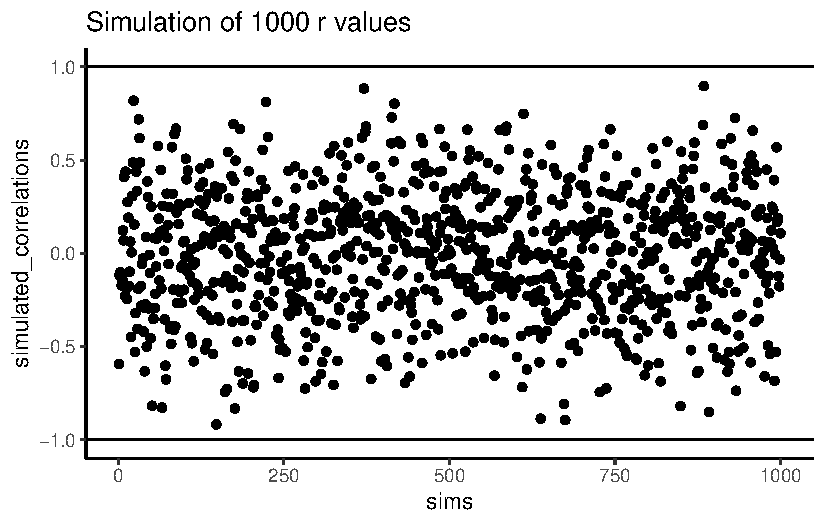
\includegraphics[width=0.75\textwidth,height=\textheight]{03-Correlation_files/figure-pdf/fig-3anotherthousand-1.pdf}

}

\caption{\label{fig-3anotherthousand}Another figure showing a range of
r-values that can be obtained by chance.}

\end{figure}

Figure~\ref{fig-3anotherthousand} shows the 1000 Pearson \(r\) values
from the simulation. Does the figure below look familiar to you? We have
already conducted a similar kind of simulation before. Each dot in the
scatter plot shows the Pearson \(r\) for each simulation from 1 to 1000.
As you can see the dots are all over of the place, in between the range
-1 to 1. The important lesson here is that random chance produced all of
these correlations. This means we can find ``correlations'' in the data
that are completely meaningless, and do not reflect any causal
relationship between one measure and another.

Let's illustrate the idea of finding ``random'' correlations one more
time, with a little movie. This time, we will show you a scatter plot of
the random values sampled for the balls chosen from the North and South
pole. If there is no relationship we should see dots going everywhere.
If there happens to be a positive relationship (purely by chance), we
should see the dots going from the bottom left to the top right. If
there happens to be a negative relationship (purely by chance), we
should see the dots going from the top left down to the bottom right.

On more thing to prepare you for the movie. There are three scatter
plots below in Figure~\ref{fig-3reminder}, showing negative, positive,
and zero correlations between two variables. You've already seen this
graph before. We are just reminding you that the blue lines are helpful
for seeing the correlation.Negative correlations occur when a line goes
down from the top left to bottom right. Positive correlations occur when
a line goes up from the bottom left to the top right. Zero correlations
occur when the line is flat (doesn't go up or down).

\begin{figure}

{\centering 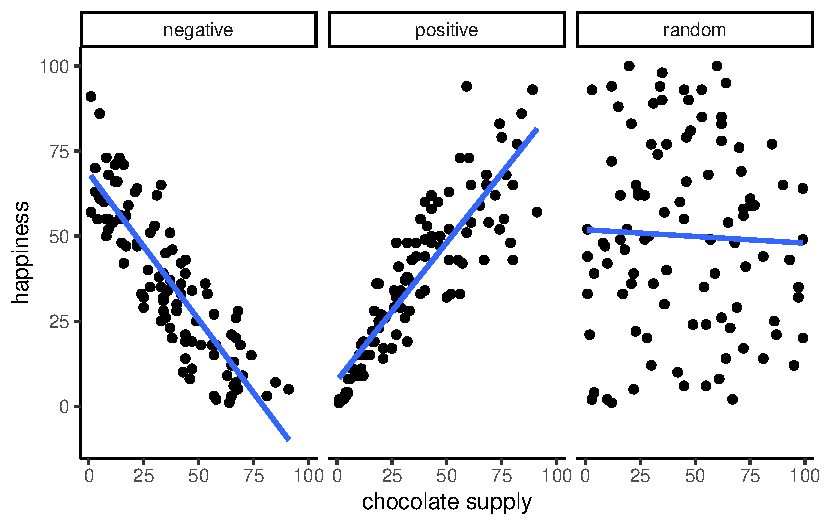
\includegraphics[width=0.75\textwidth,height=\textheight]{03-Correlation_files/figure-pdf/fig-3reminder-1.pdf}

}

\caption{\label{fig-3reminder}A reminder of what positive, negative, and
zero correlation looks like}

\end{figure}

OK, now we are ready for the movie. \textbf{?@fig-3randcor10gif} shows
the process of sampling two sets of numbers randomly, one for the X
variable, and one for the Y variable. Each time we sample 10 numbers for
each, plot them, then draw a line through them. Remember, these numbers
are all completely random, so we should expect, on average that there
should be no correlation between the numbers. However, this is not what
happens. You can the line going all over the place. Sometimes we find a
negative correlation (line goes down), sometimes we see a positive
correlation (line goes up), and sometimes it looks like zero correlation
(line is more flat).

You might be thinking this is kind of disturbing. If we know that there
should be no correlation between two random variables, how come we are
finding correlations? This is a big problem right? I mean, if someone
showed me a correlation between two things, and then claimed one thing
was related to another, how could know I if it was true. After all, it
could be chance! Chance can do that too.

Fortunately, all is not lost. We can look at our simulated data in
another way, using a histogram. Remember, just before the movie, we
simulated 1000 different correlations using random numbers. By, putting
all of those \(r\) values into a histogram, we can get a better sense of
how chance behaves. We can see what kind of correlations chance is
likely or unlikely to produce. Figure~\ref{fig-3histrandcor} is a
histogram of the simulated \(r\) values.

\begin{figure}

{\centering 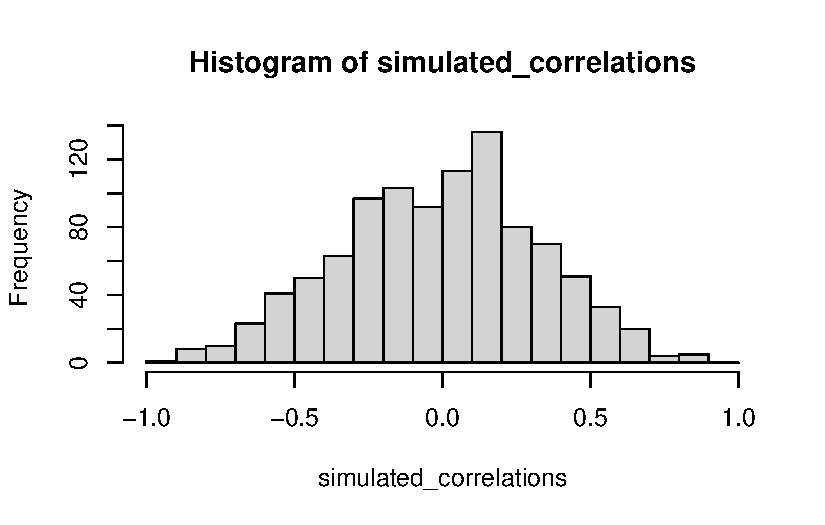
\includegraphics[width=0.75\textwidth,height=\textheight]{03-Correlation_files/figure-pdf/fig-3histrandcor-1.pdf}

}

\caption{\label{fig-3histrandcor}A histogram showing the frequency
distribution of r-values for completely random values between an X and Y
variable (sample-size=10). A rull range of r-values can be obtained by
chance alone. Larger r-values are less common than smaller r-values}

\end{figure}

Notice that this histogram is not flat. Most of the simulated \(r\)
values are close to zero. Notice, also that the bars get smaller as you
move away from zero in the positive or negative direction. The general
take home here is that chance can produce a wide range of correlations.
However, not all correlations happen very often. For example, the bars
for -1 and 1 are very small. Chance does not produce nearly perfect
correlations very often. The bars around -.5 and .5 are smaller than the
bars around zero, as medium correlations do not occur as often as small
correlations by chance alone.

You can think of this histogram as the window of chance. It shows what
chance often does, and what it often does not do. If you found a
correlation under these very same circumstances (e.g., measured the
correlation between two sets of 10 random numbers), then you could
consult this window. What should you ask the window? How about, could my
observed correlation (the one that you found in your data) have come
from this window. Let's say you found a correlation of \(r = .1\). Could
a .1 have come from the histogram? Well, look at the histogram around
where the .1 mark on the x-axis is. Is there a big bar there? If so,
this means that chance produces this value fairly often. You might be
comfortable with the inference: Yes, this .1 could have been produced by
chance, because it is well inside the window of chance. How about
\(r = .5\)? The bar is much smaller here, you might think, ``well, I can
see that chance does produce .5 some times, so chance could have
produced my .5. Did it? Maybe, maybe not, not sure''. Here, your
confidence in a strong inference about the role of chance might start
getting a bit shakier.

How about an \(r = .95\)?. You might see that the bar for .95 is very
very small, perhaps too small to see. What does this tell you? It tells
you that chance does not produce .95 very often, hardly if at all,
pretty much never. So, if you found a .95 in your data, what would you
infer? Perhaps you would be comfortable inferring that chance did not
produce your .95, after .95 is mostly outside the window of chance.

\hypertarget{increasing-sample-size-decreases-opportunity-for-spurious-correlation}{%
\subsubsection{Increasing sample-size decreases opportunity for spurious
correlation}\label{increasing-sample-size-decreases-opportunity-for-spurious-correlation}}

Before moving on, let's do one more thing with correlations. In our
pretend lottery game, each participant only sampled 10 balls each. We
found that this could lead to a range of correlations between the
numbers randomly drawn from either sides of the pole. Indeed, we even
found some correlations that were medium to large in size. If you were a
researcher who found such correlations, you might be tempted to believe
there was a relationship between your measurements. However, we know in
our little game, that those correlations would be spurious, just a
product of random sampling.

The good news is that, as a researcher, you get to make the rules of the
game. You get to determine how chance can play. This is all a little bit
metaphorical, so let's make it concrete.

We will see what happens in four different scenarios. First, we will
repeat what we already did. Each participant will draw 10 balls, then we
compute the correlation, and do this over 1000 times and look at a
histogram. Second, we will change the game so each participant draws 50
balls each, and then repeat our simulation. Third, and fourth, we will
change the game so each participant draws 100 balls each, and then 1000
balls each, and repeat etc.

Figure~\ref{fig-3corrandN} shows four different histograms of the
Pearson \(r\) values in each of the different scenarios. Each scenario
involves a different sample-size, from, 10, 50, 100 to 1000.

\begin{figure}

{\centering 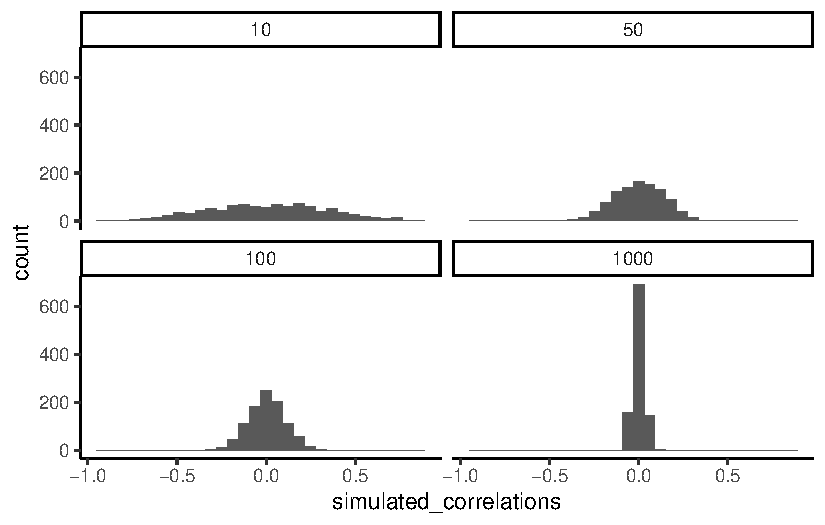
\includegraphics[width=0.75\textwidth,height=\textheight]{03-Correlation_files/figure-pdf/fig-3corrandN-1.pdf}

}

\caption{\label{fig-3corrandN}Four histograms showing the frequency
distributions of r-values between completely random X and Y variables as
a function of sample-size. The width of the distributions shrink as
sample-size increases. Smaller sample-sizes are more likely to produce a
wider range of r-values by chance. Larger sample-sizes always produce a
narrow range of small r-values}

\end{figure}

By inspecting the four histograms you should notice a clear pattern. The
width or range of each histogram shrinks as the sample-size increases.
What is going on here? Well, we already know that we can think of these
histograms as windows of chance. They tell us which \(r\) values occur
fairly often, which do not. When our sample-size is 10, lots of
different \(r\) values happen. That histogram is very flat and spread
out. However, as the sample-size increases, we see that the window of
chance gets pulled in. For example, by the time we get to 1000 balls
each, almost all of the Pearson \(r\) values are very close to 0.

One take home here, is that increasing sample-size narrows the window of
chance. So, for example, if you ran a study involving 1000 samples of
two measures, and you found a correlation of .5, then you can clearly
see in the bottom right histogram that .5 does not occur very often by
chance alone. In fact, there is no bar, because it didn't happen even
once in the simulation. As a result, when you have a large sample size
like n = 1000, you might be more confident that your observed
correlation (say of .5) was not a spurious correlation. If chance is not
producing your result, then something else is.

Finally, notice how your confidence about whether or not chance is
mucking about with your results depends on your sample size. If you only
obtained 10 samples per measurement, and found \(r = .5\), you should
not be as confident that your correlation reflects a real relationship.
Instead, you can see that \(r\)'s of .5 happen fairly often by chance
alone.

\begin{quote}
Pro tip: when you run an experiment you get to decide how many samples
you will collect, which means you can choose to narrow the window of
chance. Then, if you find a relationship in the data you can be more
confident that your finding is real, and not just something that
happened by chance.
\end{quote}

\hypertarget{some-more-movies}{%
\subsection{Some more movies}\label{some-more-movies}}

Let's ingrain these idea with some more movies. When our sample-size is
small (N is small), sampling error can cause all sort ``patterns'' in
the data. This makes it possible, and indeed common, for
``correlations'' to occur between two sets of numbers. When we increase
the sample-size, sampling error is reduced, making it less possible for
``correlations'' to occur just by chance alone. When N is large, chance
has less of an opportunity to operate.

\hypertarget{watching-how-correlation-behaves-when-there-is-no-correlation}{%
\subsubsection{Watching how correlation behaves when there is no
correlation}\label{watching-how-correlation-behaves-when-there-is-no-correlation}}

Below we randomly sample numbers for two variables, plot them, and show
the correlation using a line. There are four panels, each showing the
number of observations in the samples, from 10, 50, 100, to 1000 in each
sample.

Remember, because we are randomly sampling numbers, there should be no
relationship between the X and Y variables. But, as we have been
discussing, because of chance, we can sometimes observe a correlation
(due to chance). The important thing to watch is how the line behaves
across the four panels in \textbf{?@fig-3corRandfour}. The line twirls
around in all directions when the sample size is 10. It is also moves
around quite a bit when the sample size is 50 or 100. It still moves a
bit when the sample size is 1000, but much less. In all cases we expect
that the line should be flat, but every time we take new samples,
sometimes the line shows us pseudo patterns.

Which line should you trust? Well, hopefully you can see that the line
for 1000 samples is the most stable. It tends to be very flat every
time, and it does not depend so much on the particular sample. The line
with 10 observations per sample goes all over the place. The take home
here, is that if someone told you that they found a correlation, you
should want to know how many observations they hand in their sample. If
they only had 10 observations, how could you trust the claim that there
was a correlation? You can't!!! Not now that you know samples that are
that small can do all sorts of things by chance alone. If instead, you
found out the sample was very large, then you might trust that finding a
little bit more. For example, in the above movie you can see that when
there are 1000 samples, we never see a strong or weak correlation; the
line is always flat. This is because chance almost never produces strong
correlations when the sample size is very large.

In the above example, we sampled numbers random numbers from a uniform
distribution. Many examples of real-world data will come from a normal
or approximately normal distribution. We can repeat the above, but
sample random numbers from the same normal distribution. There will
still be zero actual correlation between the X and Y variables, because
everything is sampled randomly. \textbf{?@fig-3normCorfour} shows the
same behavior. The computed correlation for small sample-sizes fluctuate
wildly, and large sample sizes do not.

OK, so what do things look like when there actually is a correlation
between variables?

\hypertarget{watching-correlations-behave-when-there-really-is-a-correlation}{%
\subsubsection{Watching correlations behave when there really is a
correlation}\label{watching-correlations-behave-when-there-really-is-a-correlation}}

Sometimes there really are correlations between two variables that are
not caused by chance. \textbf{?@fig-3realcorFour} shows a movie of four
scatter plots. Each shows the correlation between two variables. Again,
we change the sample-size in steps of 10, 50 100, and 1000. The data
have been programmed to contain a real positive correlation. So, we
should expect that the line will be going up from the bottom left to the
top right. However, there is still variability in the data. So this
time, sampling error due to chance will fuzz the correlation. We know it
is there, but sometimes chance will cause the correlation to be
eliminated.

Notice that in the top left panel (sample-size = 10), the line is
twirling around much more than the other panels. Every new set of
samples produces different correlations. Sometimes, the line even goes
flat or downward. However, as we increase sample-size, we can see that
the line doesn't change very much, it is always going up showing a
positive correlation.

The main takeaway here is that even when there is a positive correlation
between two things, you might not be able to see it if your sample size
is small. For example, you might get unlucky with the one sample that
you measured. Your sample could show a negative correlation, even when
the actual correlation is positive! Unfortunately, in the real world we
usually only have the sample that we collected, so we always have to
wonder if we got lucky or unlucky. Fortunately, if you want to remove
luck, all you need to do is collect larger samples. Then you will be
much more likely to observe the real pattern, rather the pattern that
can be introduced by chance.

\hypertarget{summary-1}{%
\section{Summary}\label{summary-1}}

In this section we have talked about correlation, and started to build
some intuitions about \textbf{inferential statistics}, which is the
major topic of the remaining chapters. For now, the main ideas are:

\begin{enumerate}
\def\labelenumi{\arabic{enumi}.}
\tightlist
\item
  We can measure relationships in data using things like correlation
\item
  The correlations we measure can be produced by numerous things, so
  they are hard to to interpret
\item
  Correlations can be produced by chance, so have the potential to be
  completely meaningless.
\item
  However, we can create a model of exactly what chance can do. The
  model tells us whether chance is more or less likely to produce
  correlations of different sizes
\item
  We can use the chance model to help us make decisions about our own
  data. We can compare the correlation we found in our data to the
  model, then ask whether or not chance could have or was likely to have
  produced our results.
\end{enumerate}

\bookmarksetup{startatroot}

\hypertarget{probability-sampling-and-estimation}{%
\chapter{Probability, Sampling, and
Estimation}\label{probability-sampling-and-estimation}}

Sections 4.1 \& 4.9 - Adapted text by Danielle Navarro Section 4.10 -
4.11 \& 4.13 - Mix of Matthew Crump \& Danielle Navarro Section 4.12 -
4.13 - Adapted text by Danielle Navarro, all sections modified by
Mallory Barnes.

\hfill\break

\begin{quote}
I have studied many languages-French, Spanish and a little Italian, but
no one told me that Statistics was a foreign language. ---Charmaine J.
Forde
\end{quote}

Up to this point in the book, we've discussed some of the key ideas in
experimental design, and we've talked a little about how you can
summarize a data set. To a lot of people, this is all there is to
statistics: it's about calculating averages, collecting all the numbers,
drawing pictures, and putting them all in a report somewhere. Kind of
like stamp collecting, but with numbers. However, statistics covers much
more than that. In fact, descriptive statistics is one of the smallest
parts of statistics, and one of the least powerful. The bigger and more
useful part of statistics is that it provides tools \textbf{that let you
make inferences about data}.

Once you start thinking about statistics in these terms -- that
statistics is there to help us draw inferences from data -- you start
seeing examples of it everywhere. For instance, here's a tiny extract
from a newspaper article in the Sydney Morning Herald (30 Oct 2010):

\begin{quote}
``I have a tough job,'' the Premier said in response to a poll which
found her government is now the most unpopular Labor administration in
polling history, with a primary vote of just 23 per cent.
\end{quote}

This kind of remark is entirely unremarkable in the papers or in
everyday life, but let's have a think about what it entails. A polling
company has conducted a survey, usually a pretty big one because they
can afford it. I'm too lazy to track down the original survey, so let's
just imagine that they called 1000 voters at random, and 230 (23\%) of
those claimed that they intended to vote for the party. For the 2010
Federal election, the Australian Electoral Commission reported 4,610,795
enrolled voters in New South Whales; so the opinions of the remaining
4,609,795 voters (about 99.98\% of voters) remain unknown to us. Even
assuming that no-one lied to the polling company the only thing we can
say with 100\% confidence is that the true primary vote is somewhere
between 230/4610795 (about 0.005\%) and 4610025/4610795 (about 99.83\%).
So, on what basis is it legitimate for the polling company, the
newspaper, and the readership to conclude that the ALP primary vote is
only about 23\%?

The answer to the question is pretty obvious: if I call 1000 people at
random, and 230 of them say they intend to vote for the ALP, then it
seems very unlikely that these are the \textbf{only} 230 people out of
the entire voting public who actually intend to do so. In other words,
we assume that the data collected by the polling company is pretty
representative of the population at large. But how representative? Would
we be surprised to discover that the true ALP primary vote is actually
24\%? 29\%? 37\%? At this point everyday intuition starts to break down
a bit. No-one would be surprised by 24\%, and everybody would be
surprised by 37\%, but it's a bit hard to say whether 29\% is plausible.
We need some more powerful tools than just looking at the numbers and
guessing.

\textbf{Inferential statistics} provides the tools that we need to
answer these sorts of questions, and since these kinds of questions lie
at the heart of the scientific enterprise, they take up the lions share
of every introductory course on statistics and research methods.
However, our tools for making statistical inferences are 1) built on top
of \textbf{probability theory}, and 2) require an understanding of how
samples behave when you take them from distributions (defined by
probability theory\ldots). So, this chapter has two main parts. A brief
introduction to probability theory, and an introduction to sampling from
distributions.

\hypertarget{how-are-probability-and-statistics-different}{%
\section{How are probability and statistics
different?}\label{how-are-probability-and-statistics-different}}

Before we start talking about probability theory, it's helpful to spend
a moment thinking about the relationship between probability and
statistics. The two disciplines are closely related but they're not
identical. Probability theory is ``the doctrine of chances''. It's a
branch of mathematics that tells you how often different kinds of events
will happen. For example, all of these questions are things you can
answer using probability theory:

\begin{itemize}
\item
  What are the chances of a fair coin coming up heads 10 times in a row?
\item
  If I roll two six sided dice, how likely is it that I'll roll two
  sixes?
\item
  How likely is it that five cards drawn from a perfectly shuffled deck
  will all be hearts?
\item
  What are the chances that I'll win the lottery?
\end{itemize}

Notice that all of these questions have something in common. In each
case the ``truth of the world'' is known, and my question relates to the
``what kind of events'' will happen. In the first question I
\textbf{know} that the coin is fair, so there's a 50\% chance that any
individual coin flip will come up heads. In the second question, I
\textbf{know} that the chance of rolling a 6 on a single die is 1 in 6.
In the third question I \textbf{know} that the deck is shuffled
properly. And in the fourth question, I \textbf{know} that the lottery
follows specific rules. You get the idea. The critical point is that
probabilistic questions start with a known \emph{model} of the world,
and we use that model to do some calculations.

The underlying model can be quite simple. For instance, in the coin
flipping example, we can write down the model like this:
\(P(\mbox{heads}) = 0.5\) which you can read as ``the probability of
heads is 0.5''.

As we'll see later, in the same way that percentages are numbers that
range from 0\% to 100\%, probabilities are just numbers that range from
0 to 1. When using this probability model to answer the first question,
I don't actually know exactly what's going to happen. Maybe I'll get 10
heads, like the question says. But maybe I'll get three heads. That's
the key thing: in probability theory, the \textbf{model} is known, but
the \textbf{data} are not.

So that's probability. What about statistics? Statistical questions work
the other way around. In statistics, we know the truth about the world.
All we have is the data, and it is from the data that we want to
\textbf{learn} the truth about the world. Statistical questions tend to
look more like these:

\begin{itemize}
\item
  If my friend flips a coin 10 times and gets 10 heads, are they playing
  a trick on me?
\item
  If five cards off the top of the deck are all hearts, how likely is it
  that the deck was shuffled?
\item
  If the lottery commissioner's spouse wins the lottery, how likely is
  it that the lottery was rigged?
\end{itemize}

This time around, the only thing we have are data. What I \textbf{know}
is that I saw my friend flip the coin 10 times and it came up heads
every time. And what I want to \emph{infer} is whether or not I should
conclude that what I just saw was actually a fair coin being flipped 10
times in a row, or whether I should suspect that my friend is playing a
trick on me. The data I have look like this:

\begin{verbatim}
H H H H H H H H H H H
\end{verbatim}

and what I'm trying to do is work out which ``model of the world'' I
should put my trust in. If the coin is fair, then the model I should
adopt is one that says that the probability of heads is 0.5; that is,
\(P(\mbox{heads}) = 0.5\). If the coin is not fair, then I should
conclude that the probability of heads is \textbf{not} 0.5, which we
would write as \(P(\mbox{heads}) \neq 0.5\). In other words, the
statistical inference problem is to figure out which of these
probability models is right. Clearly, the statistical question isn't the
same as the probability question, but they're deeply connected to one
another. Because of this, a good introduction to statistical theory will
start with a discussion of what probability is and how it works.

\hypertarget{what-does-probability-mean}{%
\section{What does probability mean?}\label{what-does-probability-mean}}

Let's start with the first of these questions. What is ``probability''?
It might seem surprising to you, but while statisticians and
mathematicians (mostly) agree on what the \textbf{rules} of probability
are, there's much less of a consensus on what the word really
\textbf{means}. It seems weird because we're all very comfortable using
words like ``chance'', ``likely'', ``possible'' and ``probable'', and it
doesn't seem like it should be a very difficult question to answer. If
you had to explain ``probability'' to a five year old, you could do a
pretty good job. But if you've ever had that experience in real life,
you might walk away from the conversation feeling like you didn't quite
get it right, and that (like many everyday concepts) it turns out that
you don't \textbf{really} know what it's all about.

So I'll have a go at it. Let's suppose I want to bet on a soccer game
between two teams of robots, \textbf{Arduino Arsenal} and \textbf{C
Milan}. After thinking about it, I decide that there is an 80\%
probability that \textbf{Arduino Arsenal} winning. What do I mean by
that? Here are three possibilities\ldots{}

\begin{itemize}
\item
  They're robot teams, so I can make them play over and over again, and
  if I did that, \textbf{Arduino Arsenal} would win 8 out of every 10
  games on average.
\item
  For any given game, I would only agree that betting on this game is
  only ``fair'' if a \$1 bet on \textbf{C Milan} gives a \$5 payoff
  (i.e.~I get my \$1 back plus a \$4 reward for being correct), as would
  a \$4 bet on \textbf{Arduino Arsenal} (i.e., my \$4 bet plus a \$1
  reward).
\item
  My subjective ``belief'' or ``confidence'' in an \textbf{Arduino
  Arsenal} victory is four times as strong as my belief in a \textbf{C
  Milan} victory.
\end{itemize}

Each of these seems sensible. However they're not identical, and not
every statistician would endorse all of them. The reason is that there
are different statistical ideologies (yes, really!) and depending on
which one you subscribe to, you might say that some of those statements
are meaningless or irrelevant. In this section, I give a brief
introduction the two main approaches that exist in the literature. These
are by no means the only approaches, but they're the two big ones.

\hypertarget{the-frequentist-view}{%
\subsection{The frequentist view}\label{the-frequentist-view}}

The first of the two major approaches to probability, and the more
dominant one in statistics, is referred to as the \emph{frequentist
view}, and it defines probability as a \emph{long-run frequency}.
Suppose we were to try flipping a fair coin, over and over again. By
definition, this is a coin that has \(P(H) = 0.5\). What might we
observe? One possibility is that the first 20 flips might look like
this:

\begin{verbatim}
T,H,H,H,H,T,T,H,H,H,H,T,H,H,T,T,T,T,T,H
\end{verbatim}

In this case 11 of these 20 coin flips (55\%) came up heads. Now suppose
that I'd been keeping a running tally of the number of heads (which I'll
call \(N_H\)) that I've seen, across the first \(N\) flips, and
calculate the proportion of heads \(N_H / N\) every time. Here's what
I'd get (I did literally flip coins to produce this!):

\begin{longtable}[]{@{}
  >{\raggedright\arraybackslash}p{(\columnwidth - 20\tabcolsep) * \real{0.2537}}
  >{\centering\arraybackslash}p{(\columnwidth - 20\tabcolsep) * \real{0.0746}}
  >{\centering\arraybackslash}p{(\columnwidth - 20\tabcolsep) * \real{0.0746}}
  >{\centering\arraybackslash}p{(\columnwidth - 20\tabcolsep) * \real{0.0746}}
  >{\centering\arraybackslash}p{(\columnwidth - 20\tabcolsep) * \real{0.0746}}
  >{\centering\arraybackslash}p{(\columnwidth - 20\tabcolsep) * \real{0.0746}}
  >{\centering\arraybackslash}p{(\columnwidth - 20\tabcolsep) * \real{0.0746}}
  >{\centering\arraybackslash}p{(\columnwidth - 20\tabcolsep) * \real{0.0746}}
  >{\centering\arraybackslash}p{(\columnwidth - 20\tabcolsep) * \real{0.0746}}
  >{\centering\arraybackslash}p{(\columnwidth - 20\tabcolsep) * \real{0.0746}}
  >{\centering\arraybackslash}p{(\columnwidth - 20\tabcolsep) * \real{0.0746}}@{}}
\toprule\noalign{}
\endhead
\bottomrule\noalign{}
\endlastfoot
number of flips & 1 & 2 & 3 & 4 & 5 & 6 & 7 & 8 & 9 & 10 \\
number of heads & 0 & 1 & 2 & 3 & 4 & 4 & 4 & 5 & 6 & 7 \\
proportion & .00 & .50 & .67 & .75 & .80 & .67 & .57 & .63 & .67 &
.70 \\
\end{longtable}

\begin{longtable}[]{@{}
  >{\raggedright\arraybackslash}p{(\columnwidth - 20\tabcolsep) * \real{0.2537}}
  >{\centering\arraybackslash}p{(\columnwidth - 20\tabcolsep) * \real{0.0746}}
  >{\centering\arraybackslash}p{(\columnwidth - 20\tabcolsep) * \real{0.0746}}
  >{\centering\arraybackslash}p{(\columnwidth - 20\tabcolsep) * \real{0.0746}}
  >{\centering\arraybackslash}p{(\columnwidth - 20\tabcolsep) * \real{0.0746}}
  >{\centering\arraybackslash}p{(\columnwidth - 20\tabcolsep) * \real{0.0746}}
  >{\centering\arraybackslash}p{(\columnwidth - 20\tabcolsep) * \real{0.0746}}
  >{\centering\arraybackslash}p{(\columnwidth - 20\tabcolsep) * \real{0.0746}}
  >{\centering\arraybackslash}p{(\columnwidth - 20\tabcolsep) * \real{0.0746}}
  >{\centering\arraybackslash}p{(\columnwidth - 20\tabcolsep) * \real{0.0746}}
  >{\centering\arraybackslash}p{(\columnwidth - 20\tabcolsep) * \real{0.0746}}@{}}
\toprule\noalign{}
\endhead
\bottomrule\noalign{}
\endlastfoot
number of flips & 11 & 12 & 13 & 14 & 15 & 16 & 17 & 18 & 19 & 20 \\
number of heads & 8 & 8 & 9 & 10 & 10 & 10 & 10 & 10 & 10 & 11 \\
proportion & .73 & .67 & .69 & .71 & .67 & .63 & .59 & .56 & .53 &
.55 \\
\end{longtable}

Notice that at the start of the sequence, the \textbf{proportion} of
heads fluctuates wildly, starting at .00 and rising as high as .80.
Later on, one gets the impression that it dampens out a bit, with more
and more of the values actually being pretty close to the ``right''
answer of .50. This is the frequentist definition of probability in a
nutshell: flip a fair coin over and over again, and as \(N\) grows large
(approaches infinity, denoted \(N\rightarrow \infty\)), the proportion
of heads will converge to 50\%. There are some subtle technicalities
that the mathematicians care about, but qualitatively speaking, that's
how the frequentists define probability. Unfortunately, I don't have an
infinite number of coins, or the infinite patience required to flip a
coin an infinite number of times. However, I do have a computer, and
computers excel at mindless repetitive tasks. So I asked my computer to
simulate flipping a coin 1000 times, and then drew a picture of what
happens to the proportion \(N_H / N\) as \(N\) increases. Actually, I
did it four times, just to make sure it wasn't a fluke. The results are
shown in Figure~\ref{fig-4FreqProb}. As you can see, the
\textbf{proportion of observed heads} eventually stops fluctuating, and
settles down; when it does, the number at which it finally settles is
the true probability of heads.

\begin{figure}

{\centering 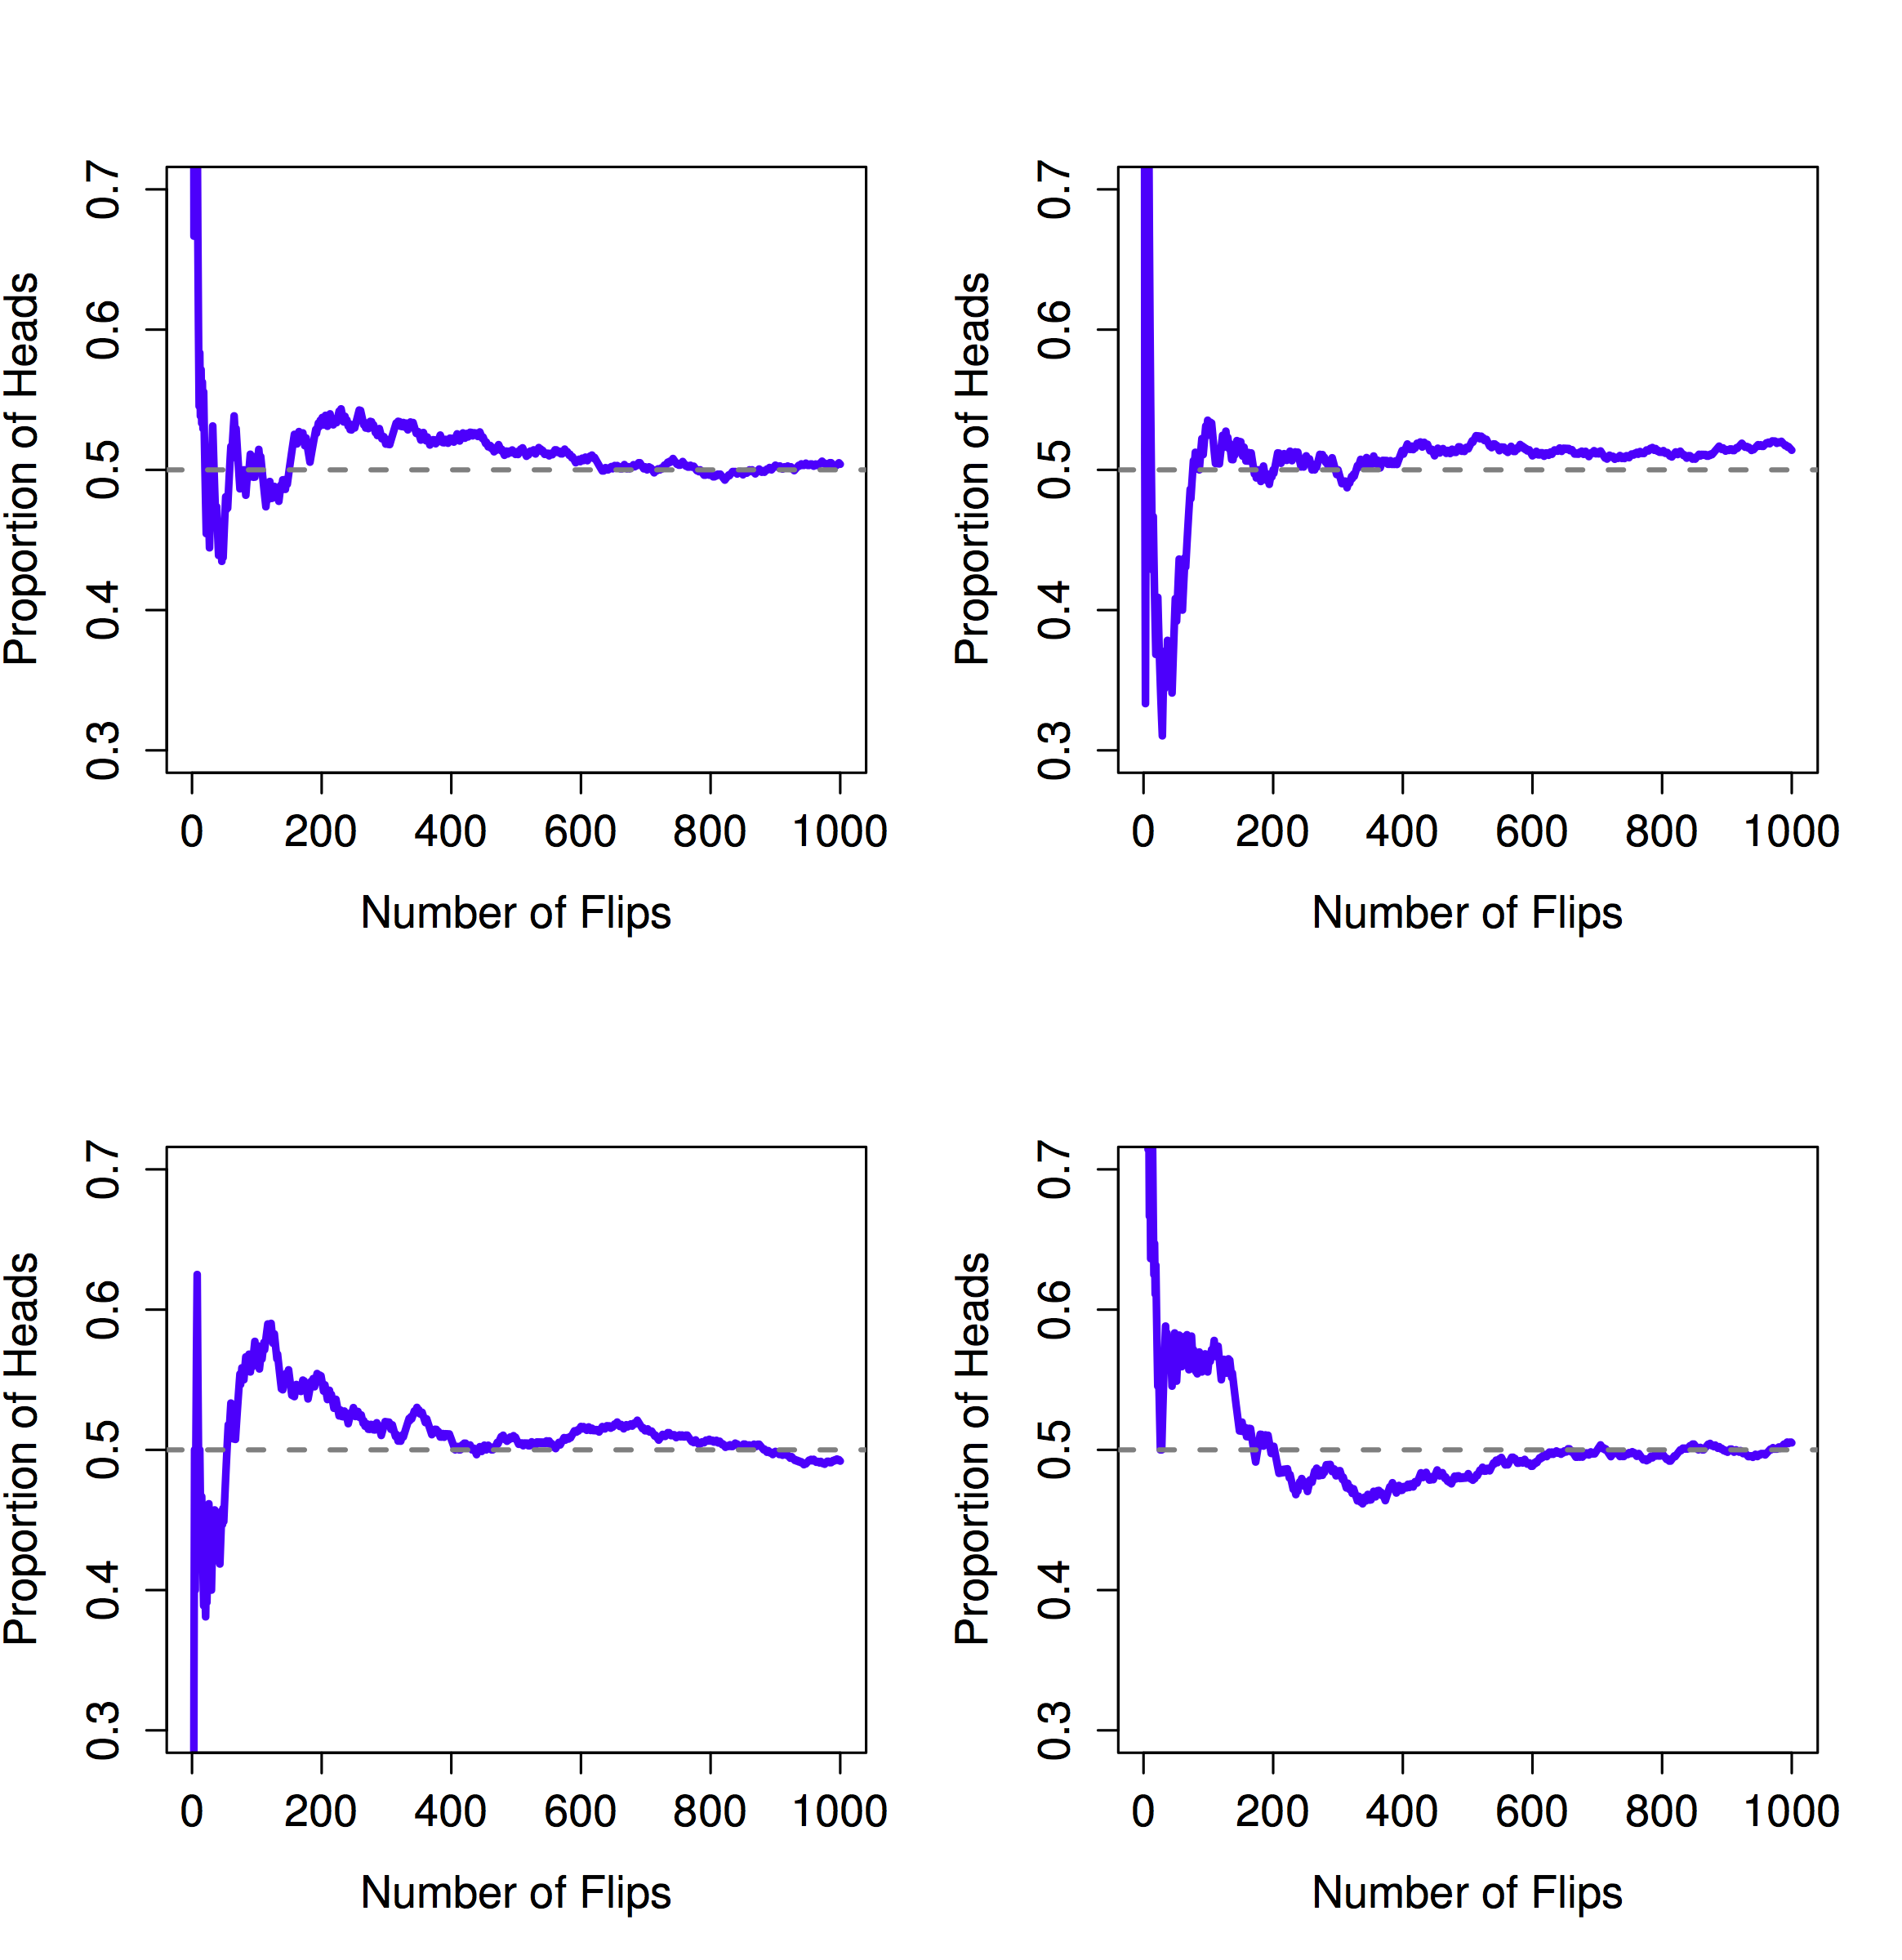
\includegraphics[width=0.75\textwidth,height=\textheight]{imgs/navarro_img/probability/frequentistProb-eps-converted-to.png}

}

\caption{\label{fig-4FreqProb}An illustration of how frequentist
probability works. If you flip a fair coin over and over again, the
proportion of heads that you've seen eventually settles down, and
converges to the true probability of 0.5. Each panel shows four
different simulated experiments: in each case, we pretend we flipped a
coin 1000 times, and kept track of the proportion of flips that were
heads as we went along. Although none of these sequences actually ended
up with an exact value of .5, if we'd extended the experiment for an
infinite number of coin flips they would have.}

\end{figure}

The frequentist definition of probability has some desirable
characteristics. First, it is objective: the probability of an event is
\textbf{necessarily} grounded in the world. The only way that
probability statements can make sense is if they refer to (a sequence
of) events that occur in the physical universe. Second, it is
unambiguous: any two people watching the same sequence of events unfold,
trying to calculate the probability of an event, must inevitably come up
with the same answer.

However, it also has undesirable characteristics. Infinite sequences
don't exist in the physical world. Suppose you picked up a coin from
your pocket and started to flip it. Every time it lands, it impacts on
the ground. Each impact wears the coin down a bit; eventually, the coin
will be destroyed. So, one might ask whether it really makes sense to
pretend that an ``infinite'' sequence of coin flips is even a meaningful
concept, or an objective one. We can't say that an ``infinite sequence''
of events is a real thing in the physical universe, because the physical
universe doesn't allow infinite anything.

More seriously, the frequentist definition has a narrow scope. There are
lots of things out there that human beings are happy to assign
probability to in everyday language, but cannot (even in theory) be
mapped onto a hypothetical sequence of events. For instance, if a
meteorologist comes on TV and says, ``the probability of rain in
Adelaide on 2 November 2048 is 60\%'' we humans are happy to accept
this. But it's not clear how to define this in frequentist terms.
There's only one city of Adelaide, and only 2 November 2048. There's no
infinite sequence of events here, just a once-off thing. Frequentist
probability genuinely \textbf{forbids} us from making probability
statements about a single event. From the frequentist perspective, it
will either rain tomorrow or it will not; there is no ``probability''
that attaches to a single non-repeatable event. Now, it should be said
that there are some very clever tricks that frequentists can use to get
around this. One possibility is that what the meteorologist means is
something like this: ``There is a category of days for which I predict a
60\% chance of rain; if we look only across those days for which I make
this prediction, then on 60\% of those days it will actually rain''.
It's very weird and counter intuitive to think of it this way, but you
do see frequentists do this sometimes.

\hypertarget{the-bayesian-view}{%
\subsection{The Bayesian view}\label{the-bayesian-view}}

The \textbf{Bayesian view} of probability is often called the
subjectivist view, and it is a minority view among statisticians, but
one that has been steadily gaining traction for the last several
decades. There are many flavors of Bayesianism, making hard to say
exactly what ``the'' Bayesian view is. The most common way of thinking
about subjective probability is to define the probability of an event as
the \textbf{degree of belief} that an intelligent and rational agent
assigns to that truth of that event. From that perspective,
probabilities don't exist in the world, but rather in the thoughts and
assumptions of people and other intelligent beings. However, in order
for this approach to work, we need some way of operationalising ``degree
of belief''. One way that you can do this is to formalize it in terms of
``rational gambling'', though there are many other ways. Suppose that I
believe that there's a 60\% probability of rain tomorrow. If someone
offers me a bet: if it rains tomorrow, then I win \$5, but if it doesn't
rain then I lose \$5. Clearly, from my perspective, this is a pretty
good bet. On the other hand, if I think that the probability of rain is
only 40\%, then it's a bad bet to take. Thus, we can operationalize the
notion of a ``subjective probability'' in terms of what bets I'm willing
to accept.

What are the advantages and disadvantages to the Bayesian approach? The
main advantage is that it allows you to assign probabilities to any
event you want to. You don't need to be limited to those events that are
repeatable. The main disadvantage (to many people) is that we can't be
purely objective -- specifying a probability requires us to specify an
entity that has the relevant degree of belief. This entity might be a
human, an alien, a robot, or even a statistician, but there has to be an
intelligent agent out there that believes in things. To many people this
is uncomfortable: it seems to make probability arbitrary. While the
Bayesian approach does require that the agent in question be rational
(i.e., obey the rules of probability), it does allow everyone to have
their own beliefs; I can believe the coin is fair and you don't have to,
even though we're both rational. The frequentist view doesn't allow any
two observers to attribute different probabilities to the same event:
when that happens, then at least one of them must be wrong. The Bayesian
view does not prevent this from occurring. Two observers with different
background knowledge can legitimately hold different beliefs about the
same event. In short, where the frequentist view is sometimes considered
to be too narrow (forbids lots of things that that we want to assign
probabilities to), the Bayesian view is sometimes thought to be too
broad (allows too many differences between observers).

\hypertarget{whats-the-difference-and-who-is-right}{%
\subsection{What's the difference? And who is
right?}\label{whats-the-difference-and-who-is-right}}

Now that you've seen each of these two views independently, it's useful
to make sure you can compare the two. Go back to the hypothetical robot
soccer game at the start of the section. What do you think a frequentist
and a Bayesian would say about these three statements? Which statement
would a frequentist say is the correct definition of probability? Which
one would a Bayesian do? Would some of these statements be meaningless
to a frequentist or a Bayesian? If you've understood the two
perspectives, you should have some sense of how to answer those
questions.

Okay, assuming you understand the different, you might be wondering
which of them is \textbf{right}? Honestly, I don't know that there is a
right answer. As far as I can tell there's nothing mathematically
incorrect about the way frequentists think about sequences of events,
and there's nothing mathematically incorrect about the way that
Bayesians define the beliefs of a rational agent. In fact, when you dig
down into the details, Bayesians and frequentists actually agree about a
lot of things. Many frequentist methods lead to decisions that Bayesians
agree a rational agent would make. Many Bayesian methods have very good
frequentist properties.

For the most part, I'm a pragmatist so I'll use any statistical method
that I trust. As it turns out, that makes me prefer Bayesian methods,
for reasons I'll explain towards the end of the book, but I'm not
fundamentally opposed to frequentist methods. Not everyone is quite so
relaxed. For instance, consider Sir Ronald Fisher, one of the towering
figures of 20th century statistics and a vehement opponent to all things
Bayesian, whose paper on the mathematical foundations of statistics
referred to Bayesian probability as ``an impenetrable jungle {[}that{]}
arrests progress towards precision of statistical concepts'' Fisher
(1922, 311). Or the psychologist Paul Meehl, who suggests that relying
on frequentist methods could turn you into ``a potent but sterile
intellectual rake who leaves in his merry path a long train of ravished
maidens but no viable scientific offspring'' Meehl (1967, 114). The
history of statistics, as you might gather, is not devoid of
entertainment.

\hypertarget{basic-probability-theory}{%
\section{Basic probability theory}\label{basic-probability-theory}}

Ideological arguments between Bayesians and frequentists
notwithstanding, it turns out that people mostly agree on the rules that
probabilities should obey. There are lots of different ways of arriving
at these rules. The most commonly used approach is based on the work of
Andrey Kolmogorov, one of the great Soviet mathematicians of the 20th
century. I won't go into a lot of detail, but I'll try to give you a bit
of a sense of how it works. And in order to do so, I'm going to have to
talk about my pants.

\hypertarget{introducing-probability-distributions}{%
\subsection{Introducing probability
distributions}\label{introducing-probability-distributions}}

One of the disturbing truths about my life is that I only own 5 pairs of
pants: three pairs of jeans, the bottom half of a suit, and a pair of
tracksuit pants. Even sadder, I've given them names: I call them
\(X_1\), \(X_2\), \(X_3\), \(X_4\) and \(X_5\). I really do: that's why
they call me Mister Imaginative. Now, on any given day, I pick out
exactly one of pair of pants to wear. Not even I'm so stupid as to try
to wear two pairs of pants, and thanks to years of training I never go
outside without wearing pants anymore. If I were to describe this
situation using the language of probability theory, I would refer to
each pair of pants (i.e., each \(X\)) as an \emph{elementary event}. The
key characteristic of elementary events is that every time we make an
observation (e.g., every time I put on a pair of pants), then the
outcome will be one and only one of these events. Like I said, these
days I always wear exactly one pair of pants, so my pants satisfy this
constraint. Similarly, the set of all possible events is called a
\emph{sample space}. Granted, some people would call it a ``wardrobe'',
but that's because they're refusing to think about my pants in
probabilistic terms. Sad.

Okay, now that we have a sample space (a wardrobe), which is built from
lots of possible elementary events (pants), what we want to do is assign
a \emph{probability} of one of these elementary events. For an event
\(X\), the probability of that event \(P(X)\) is a number that lies
between 0 and 1. The bigger the value of \(P(X)\), the more likely the
event is to occur. So, for example, if \(P(X) = 0\), it means the event
\(X\) is impossible (i.e., I never wear those pants). On the other hand,
if \(P(X) = 1\) it means that event \(X\) is certain to occur (i.e., I
always wear those pants). For probability values in the middle, it means
that I sometimes wear those pants. For instance, if \(P(X) = 0.5\) it
means that I wear those pants half of the time.

At this point, we're almost done. The last thing we need to recognize is
that ``something always happens''. Every time I put on pants, I really
do end up wearing pants (crazy, right?). What this somewhat trite
statement means, in probabilistic terms, is that the probabilities of
the elementary events need to add up to 1. This is known as the
\emph{law of total probability}, not that any of us really care. More
importantly, if these requirements are satisfied, then what we have is a
\emph{probability distribution}. For example, this is an example of a
probability distribution

\begin{longtable}[]{@{}lcc@{}}
\toprule\noalign{}
Which pants? & Label & Probability \\
\midrule\noalign{}
\endhead
\bottomrule\noalign{}
\endlastfoot
Blue jeans & \(X_1\) & \(P(X_1) = .5\) \\
Grey jeans & \(X_2\) & \(P(X_2) = .3\) \\
Black jeans & \(X_3\) & \(P(X_3) = .1\) \\
Black suit & \(X_4\) & \(P(X_4) = 0\) \\
Blue tracksuit & \(X_5\) & \(P(X_5) = .1\) \\
\end{longtable}

Each of the events has a probability that lies between 0 and 1, and if
we add up the probability of all events, they sum to 1. Awesome. We can
even draw a nice bar graph to visualize this distribution, as shown in
Figure~\ref{fig-4pantsprob}. And at this point, we've all achieved
something. You've learned what a probability distribution is, and I've
finally managed to find a way to create a graph that focuses entirely on
my pants. Everyone wins!

\begin{figure}

{\centering 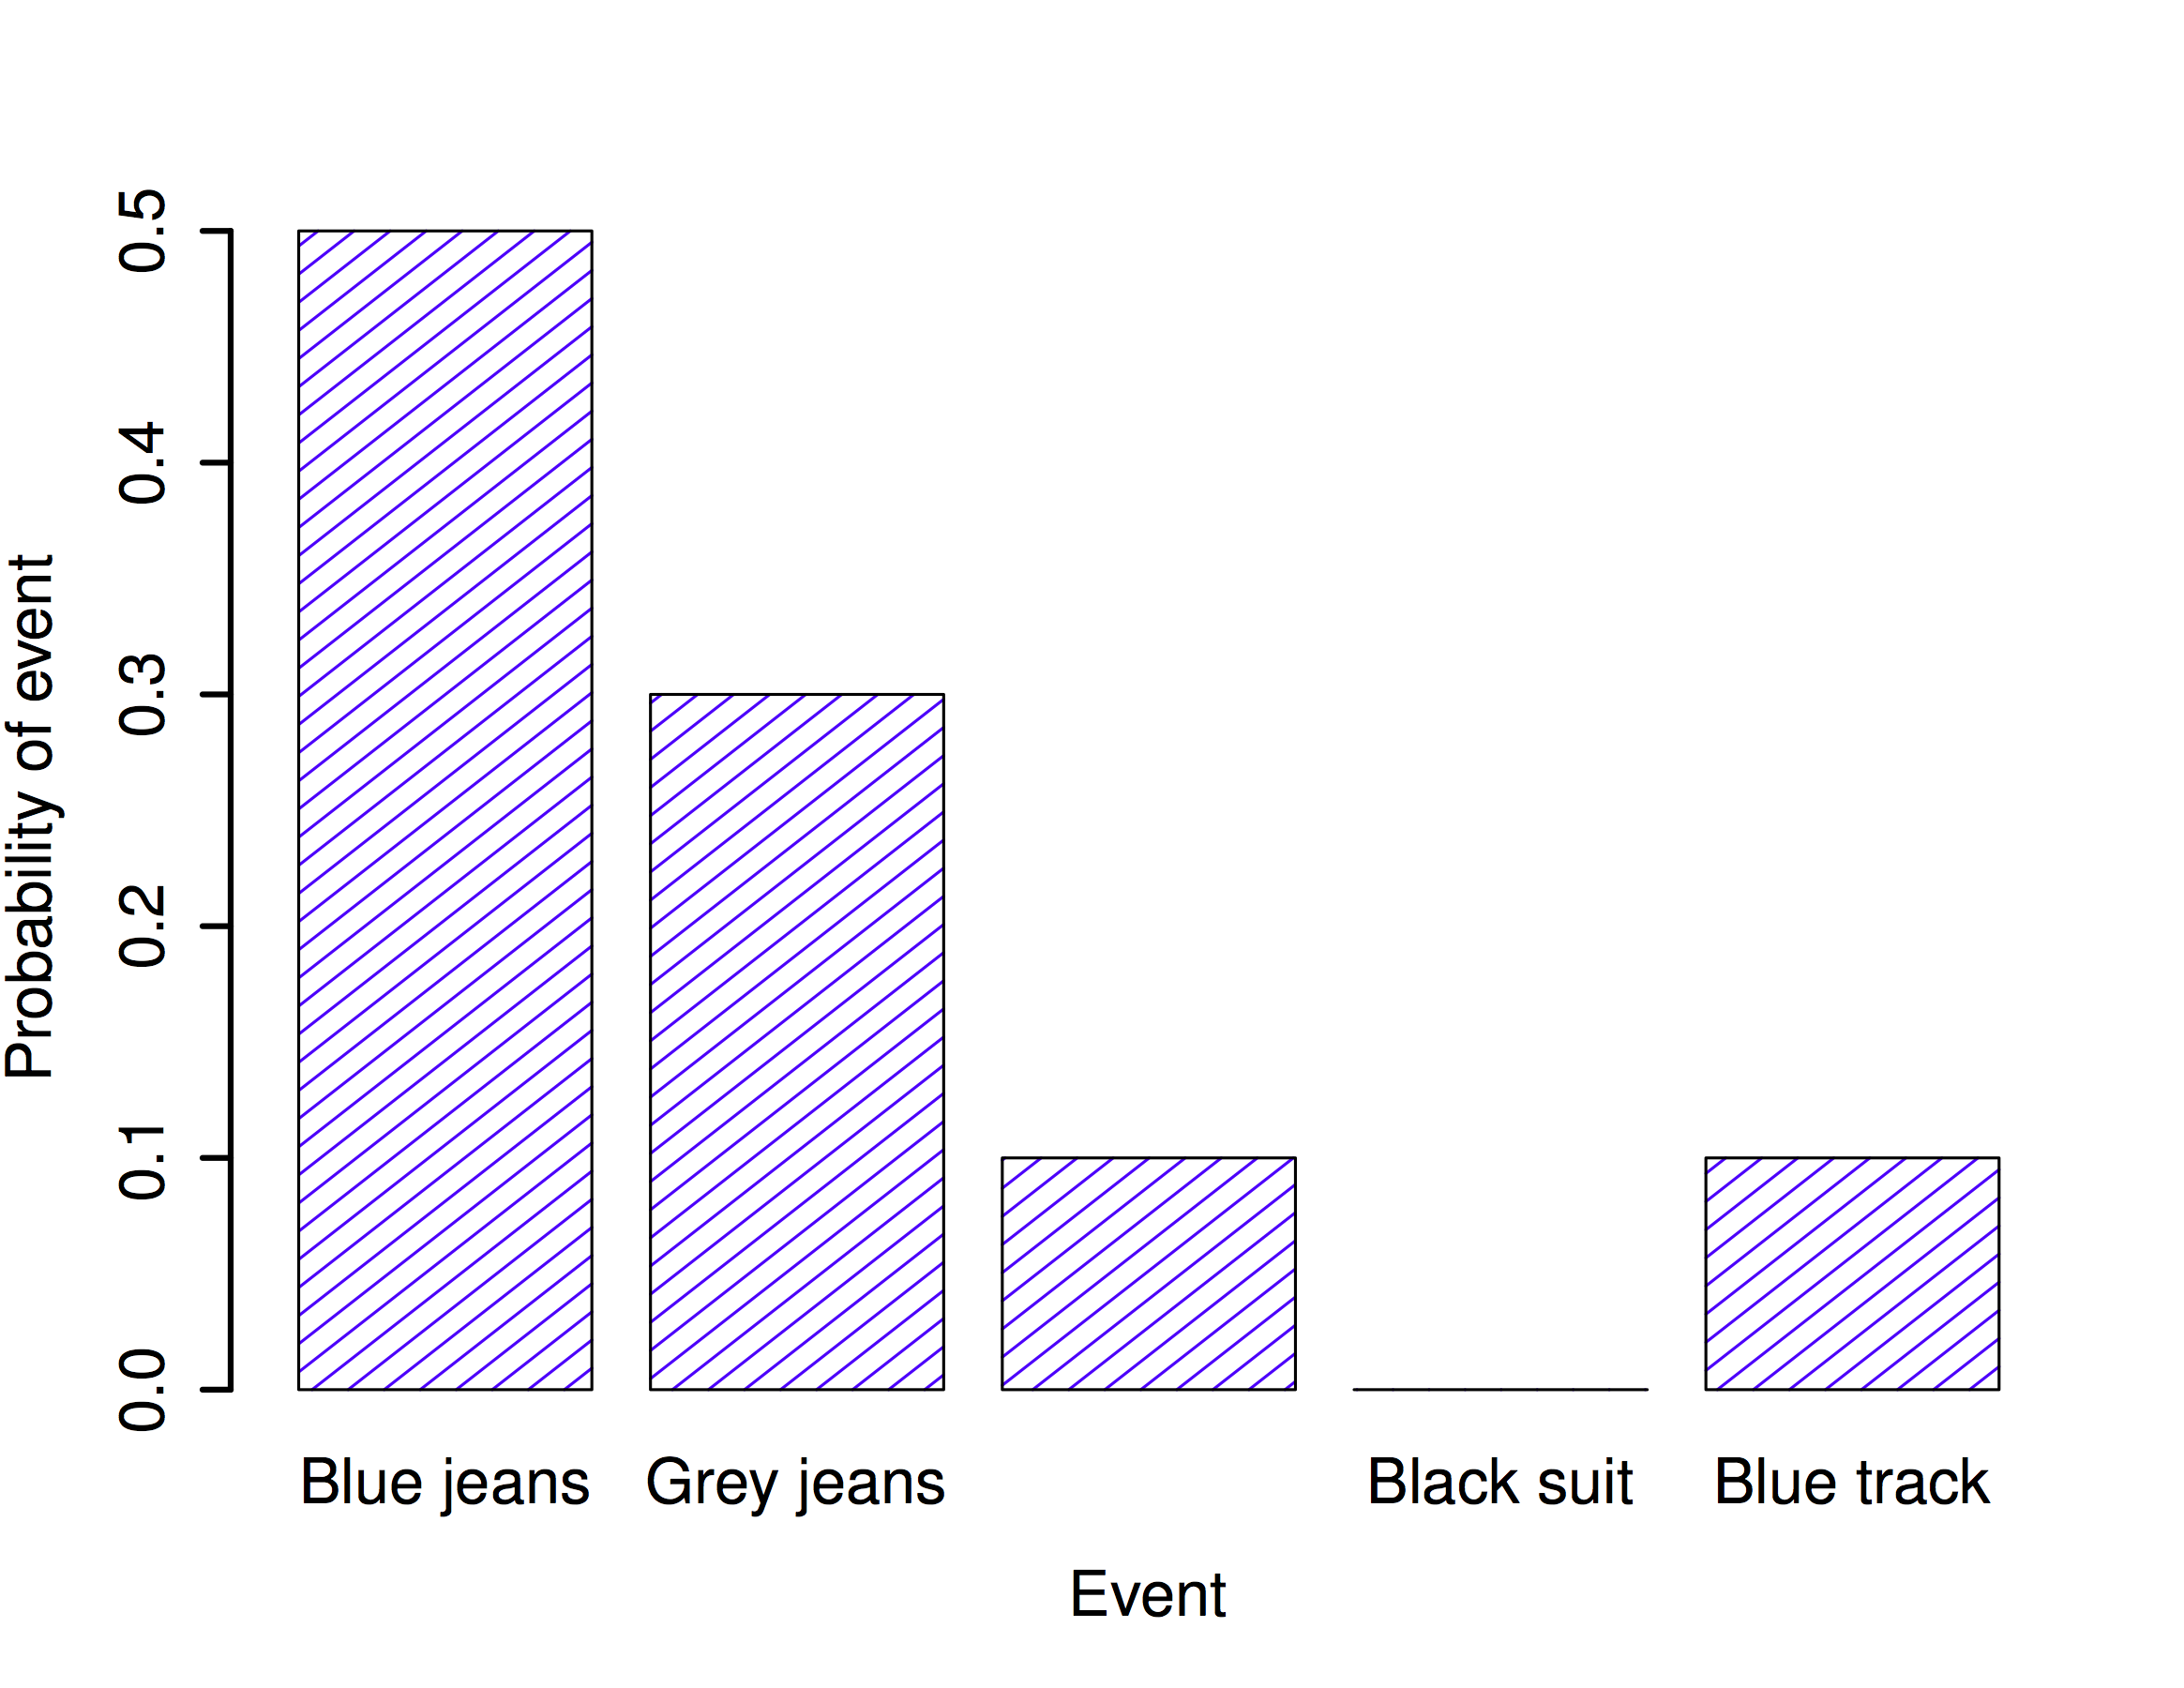
\includegraphics[width=0.75\textwidth,height=\textheight]{imgs/navarro_img/probability/pantsDistribution-eps-converted-to.png}

}

\caption{\label{fig-4pantsprob}A visual depiction of the pants
probability distribution. There are five elementary events,
corresponding to the five pairs of pants that I own. Each event has some
probability of occurring: this probability is a number between 0 to 1.
The sum of these probabilities is 1.}

\end{figure}

The only other thing that I need to point out is that probability theory
allows you to talk about \emph{non elementary events} as well as
elementary ones. The easiest way to illustrate the concept is with an
example. In the pants example, it's perfectly legitimate to refer to the
probability that I wear jeans. In this scenario, the ``Dan wears jeans''
event said to have happened as long as the elementary event that
actually did occur is one of the appropriate ones; in this case ``blue
jeans'', ``black jeans'' or ``grey jeans''. In mathematical terms, we
defined the ``jeans'' event \(E\) to correspond to the set of elementary
events \((X_1, X_2, X_3)\). If any of these elementary events occurs,
then \(E\) is also said to have occurred. Having decided to write down
the definition of the \(E\) this way, it's pretty straightforward to
state what the probability \(P(E)\) is: we just add everything up. In
this particular case \[P(E) = P(X_1) + P(X_2) + P(X_3)\] and, since the
probabilities of blue, grey and black jeans respectively are .5, .3 and
.1, the probability that I wear jeans is equal to .9.

At this point you might be thinking that this is all terribly obvious
and simple and you'd be right. All we've really done is wrap some basic
mathematics around a few common sense intuitions. However, from these
simple beginnings it's possible to construct some extremely powerful
mathematical tools. I'm definitely not going to go into the details in
this book, but what I will do is list some of the other rules that
probabilities satisfy. These rules can be derived from the simple
assumptions that I've outlined above, but since we don't actually use
these rules for anything in this book, I won't do so here.

\begin{longtable}[]{@{}lrll@{}}
\caption{Some basic rules that probabilities must satisfy. You don't
really need to know these rules in order to understand the analyses that
we'll talk about later in the book, but they are important if you want
to understand probability theory a bit more deeply.}\tabularnewline
\toprule\noalign{}
English & Notation & & Formula \\
\midrule\noalign{}
\endfirsthead
\toprule\noalign{}
English & Notation & & Formula \\
\midrule\noalign{}
\endhead
\bottomrule\noalign{}
\endlastfoot
not \(A\) & \(P(\neg A)\) & \(=\) & \(1-P(A)\) \\
\(A\) or \(B\) & \(P(A \cup B)\) & \(=\) &
\(P(A) + P(B) - P(A \cap B)\) \\
\(A\) and \(B\) & \(P(A \cap B)\) & \(=\) & \(P(A|B) P(B)\) \\
\end{longtable}

Now that we have the ability to ``define'' non-elementary events in
terms of elementary ones, we can actually use this to construct (or, if
you want to be all mathematicallish, ``derive'') some of the other rules
of probability. These rules are listed above, and while I'm pretty
confident that very few of my readers actually care about how these
rules are constructed, I'm going to show you anyway: even though it's
boring and you'll probably never have a lot of use for these
derivations, if you read through it once or twice and try to see how it
works, you'll find that probability starts to feel a bit less
mysterious, and with any luck a lot less daunting. So here goes.
Firstly, in order to construct the rules I'm going to need a sample
space \(X\) that consists of a bunch of elementary events \(x\), and two
non-elementary events, which I'll call \(A\) and \(B\). Let's say:
\[\begin{array}{rcl}
X &=& (x_1, x_2, x_3, x_4, x_5) \\
A &=& (x_1, x_2, x_3) \\
B &=& (x_3, x_4)
\end{array}\] To make this a bit more concrete, let's suppose that we're
still talking about the pants distribution. If so, \(A\) corresponds to
the event ``jeans'', and \(B\) corresponds to the event ``black'':
\[\begin{array}{rcl}
\mbox{``jeans''} &=& (\mbox{``blue jeans''}, \mbox{``grey jeans''}, \mbox{``black jeans''}) \\
\mbox{``black''} &=& (\mbox{``black jeans''}, \mbox{``black suit''})
\end{array}\] So now let's start checking the rules that I've listed in
the table.

In the first line, the table says that \[P(\neg A) = 1- P(A)\] and what
it \textbf{means} is that the probability of ``not \(A\)'' is equal to 1
minus the probability of \(A\). A moment's thought (and a tedious
example) make it obvious why this must be true. If \(A\) corresponds to
the even that I wear jeans (i.e., one of \(x_1\) or \(x_2\) or \(x_3\)
happens), then the only meaningful definition of ``not \(A\)'' (which is
mathematically denoted as \(\neg A\)) is to say that \(\neg A\) consists
of \textbf{all} elementary events that don't belong to \(A\). In the
case of the pants distribution it means that \(\neg A = (x_4, x_5)\),
or, to say it in English: ``not jeans'' consists of all pairs of pants
that aren't jeans (i.e., the black suit and the blue tracksuit).
Consequently, every single elementary event belongs to either \(A\) or
\(\neg A\), but not both. Okay, so now let's rearrange our statement
above: \[P(\neg A) + P(A) = 1\] which is a trite way of saying either I
do wear jeans or I don't wear jeans: the probability of ``not jeans''
plus the probability of ``jeans'' is 1. Mathematically:
\[\begin{array}{rcl}
P(\neg A) &=&  P(x_4) + P(x_5) \\
P(A) &=& P(x_1) + P(x_2) + P(x_3) 
\end{array}\] so therefore \[\begin{array}{rcl} 
P(\neg A) + P(A) &=& P(x_1) + P(x_2) + P(x_3) + P(x_4) + P(x_5) \\
&=& \sum_{x \in X} P(x) \\
&=& 1
\end{array}\] Excellent. It all seems to work.

Wow, I can hear you saying. That's a lot of \(x\)s to tell me the
freaking obvious. And you're right: this \textbf{is} freaking obvious.
The whole \textbf{point} of probability theory to to formalize and
mathematize a few very basic common sense intuitions. So let's carry
this line of thought forward a bit further. In the last section I
defined an event corresponding to \textbf{not} A, which I denoted
\(\neg A\). Let's now define two new events that correspond to important
everyday concepts: \(A\) \textbf{and} \(B\), and \(A\) \textbf{or}
\(B\). To be precise:

\begin{longtable}[]{@{}lc@{}}
\toprule\noalign{}
English statement: & Mathematical notation: \\
\midrule\noalign{}
\endhead
\bottomrule\noalign{}
\endlastfoot
``\(A\) and \(B\)'' both happen & \(A \cap B\) \\
at least one of ``\(A\) or \(B\)'' happens & \(A \cup B\) \\
\end{longtable}

Since \(A\) and \(B\) are both defined in terms of our elementary events
(the \(x\)s) we're going to need to try to describe \(A \cap B\) and
\(A \cup B\) in terms of our elementary events too. Can we do this? Yes
we can The only way that both \(A\) and \(B\) can occur is if the
elementary event that we observe turns out to belong to both \(A\) and
\(B\). Thus ``\(A \cap B\)'' includes only those elementary events that
belong to both \(A\) and \(B\)\ldots{} \[\begin{array}{rcl}
A &=& (x_1, x_2, x_3) \\
B &=& (x_3, x_4) \\
A \cap B & = & (x_3) 
\end{array}\] So, um, the only way that I can wear ``jeans''
\((x_1, x_2, x_3)\) and ``black pants'' \((x_3, x_4)\) is if I wear
``black jeans'' \((x_3)\). Another victory for the bloody obvious.

At this point, you're not going to be at all shocked by the definition
of \(A \cup B\), though you're probably going to be extremely bored by
it. The only way that I can wear ``jeans'' or ``black pants'' is if the
elementary pants that I actually do wear belongs to \(A\) or to \(B\),
or to both. So\ldots{} \[\begin{array}{rcl}
A &=& (x_1, x_2, x_3) \\
B &=& (x_3, x_4) \\
A \cup B & = & (x_1, x_2, x_3, x_4) 
\end{array}\] Oh yeah baby. Mathematics at its finest.

So, we've defined what we mean by \(A \cap B\) and \(A \cup B\). Now
let's assign probabilities to these events. More specifically, let's
start by verifying the rule that claims that:
\[P(A \cup B) = P(A) + P(B) - P(A \cap B)\] Using our definitions
earlier, we know that \(A \cup B = (x_1, x_2, x_3, x_4)\), so
\[P(A \cup B) = P(x_1) + P(x_2) + P(x_3) + P(x_4)\] and making similar
use of the fact that we know what elementary events belong to \(A\),
\(B\) and \(A \cap B\)\ldots. \[\begin{array}{rcl}
P(A)  &=&   P(x_1) + P(x_2) + P(x_3)    \\
P(B) &=&  P(x_3) + P(x_4)  \\
P(A \cap B) &=&  P(x_3)
\end{array}\] and therefore \[\begin{array}{rcl}
P(A) + P(B) - P(A \cap B)
&=&  P(x_1) + P(x_2) + P(x_3) +  P(x_3) + P(x_4) -  P(x_3) \\
&=& P(x_1) + P(x_2) + P(x_3) + P(x_4) \\
&=& P(A \cup B)
\end{array}\] Done.

The next concept we need to define is the notion of ``\(B\) given
\(A\)'', which is typically written \(B | A\). Here's what I mean:
suppose that I get up one morning, and put on a pair of pants. An
elementary event \(x\) has occurred. Suppose further I yell out to my
wife (who is in the other room, and so cannot see my pants) ``I'm
wearing jeans today!''. Assuming that she believes that I'm telling the
truth, she knows that \(A\) is true. \textbf{Given} that she knows that
\(A\) has happened, what is the \textbf{conditional probability} that
\(B\) is also true? Well, let's think about what she knows. Here are the
facts:

\begin{itemize}
\item
  \textbf{The non-jeans events are impossible}. If \(A\) is true, then
  we know that the only possible elementary events that could have
  occurred are \(x_1\), \(x_2\) and \(x_3\) (i.e.,the jeans). The
  non-jeans events \(x_4\) and \(x_5\) are now impossible, and must be
  assigned probability zero. In other words, our \textbf{sample space}
  has been restricted to the jeans events. But it's still the case that
  the probabilities of these these events \textbf{must} sum to 1: we
  know for sure that I'm wearing jeans.
\item
  \textbf{She's learned nothing about which jeans I'm wearing}. Before I
  made my announcement that I was wearing jeans, she already knew that I
  was five times as likely to be wearing blue jeans (\(P(x_1) = 0.5\))
  than to be wearing black jeans (\(P(x_3) = 0.1\)). My announcement
  doesn't change this\ldots{} I said \textbf{nothing} about what color
  my jeans were, so it must remain the case that \(P(x_1) / P(x_3)\)
  stays the same, at a value of 5.
\end{itemize}

There's only one way to satisfy these constraints: set the impossible
events to have zero probability (i.e., \(P(x | A) = 0\) if \(x\) is not
in \(A\)), and then divide the probabilities of all the others by
\(P(A)\). In this case, since \(P(A) = 0.9\), we divide by 0.9. This
gives:

\begin{longtable}[]{@{}
  >{\raggedright\arraybackslash}p{(\columnwidth - 6\tabcolsep) * \real{0.2162}}
  >{\raggedright\arraybackslash}p{(\columnwidth - 6\tabcolsep) * \real{0.2432}}
  >{\centering\arraybackslash}p{(\columnwidth - 6\tabcolsep) * \real{0.2432}}
  >{\centering\arraybackslash}p{(\columnwidth - 6\tabcolsep) * \real{0.2973}}@{}}
\toprule\noalign{}
\begin{minipage}[b]{\linewidth}\raggedright
which pants?
\end{minipage} & \begin{minipage}[b]{\linewidth}\raggedright
elementary event
\end{minipage} & \begin{minipage}[b]{\linewidth}\centering
old prob, \(P(x)\)
\end{minipage} & \begin{minipage}[b]{\linewidth}\centering
new prob, \(P(x | A)\)
\end{minipage} \\
\midrule\noalign{}
\endhead
\bottomrule\noalign{}
\endlastfoot
blue jeans & \(x_1\) & 0.5 & 0.556 \\
grey jeans & \(x_2\) & 0.3 & 0.333 \\
black jeans & \(x_3\) & 0.1 & 0.111 \\
black suit & \(x_4\) & 0 & 0 \\
blue tracksuit & \(x_5\) & 0.1 & 0 \\
\end{longtable}

In mathematical terms, we say that \[P(x | A) = \frac{P(x)}{P(A)}\] if
\(x \in A\), and \(P(x|A) = 0\) otherwise. And therefore\ldots{}
\[\begin{array}{rcl}
P(B | A) &=& P(x_3 | A)  + P(x_4 | A) \\ \\
&=&  \displaystyle\frac{P(x_3)}{P(A)} + 0    \\ \\
&=& \displaystyle\frac{P(x_3)}{P(A)}
\end{array}\] Now, recalling that \(A \cap B = (x_3)\), we can write
this as \[P(B | A) = \frac{P(A \cap B)}{P(A)}\] and if we multiply both
sides by \(P(A)\) we obtain: \[P(A \cap B) = P(B| A) P(A)\] which is the
third rule that we had listed in the table.

\hypertarget{the-binomial-distribution}{%
\section{The binomial distribution}\label{the-binomial-distribution}}

As you might imagine, probability distributions vary enormously, and
there's an enormous range of distributions out there. However, they
aren't all equally important. In fact, the vast majority of the content
in this book relies on one of five distributions: the binomial
distribution, the normal distribution, the \(t\) distribution, the
\(\chi^2\) (``chi-square'') distribution and the \(F\) distribution.
Given this, what I'll do over the next few sections is provide a brief
introduction to all five of these, paying special attention to the
binomial and the normal. I'll start with the binomial distribution,
since it's the simplest of the five.

\hypertarget{introducing-the-binomial}{%
\subsection{Introducing the binomial}\label{introducing-the-binomial}}

The theory of probability originated in the attempt to describe how
games of chance work, so it seems fitting that our discussion of the
\emph{binomial distribution} should involve a discussion of rolling dice
and flipping coins. Let's imagine a simple ``experiment'': in my hand
I'm holding 20 identical six-sided dice. On one face of each die there's
a picture of a skull; the other five faces are all blank. If I proceed
to roll all 20 dice, what's the probability that I'll get exactly 4
skulls? Assuming that the dice are fair, we know that the chance of any
one die coming up skulls is 1 in 6; to say this another way, the skull
probability for a single die is approximately \(.167\). This is enough
information to answer our question, so let's have a look at how it's
done.

As usual, we'll want to introduce some names and some notation. We'll
let \(N\) denote the number of dice rolls in our experiment; which is
often referred to as the \emph{size parameter} of our binomial
distribution. We'll also use \(\theta\) to refer to the the probability
that a single die comes up skulls, a quantity that is usually called the
\emph{success probability} of the binomial. Finally, we'll use \(X\) to
refer to the results of our experiment, namely the number of skulls I
get when I roll the dice. Since the actual value of \(X\) is due to
chance, we refer to it as a \emph{random variable}. In any case, now
that we have all this terminology and notation, we can use it to state
the problem a little more precisely. The quantity that we want to
calculate is the probability that \(X = 4\) given that we know that
\(\theta = .167\) and \(N=20\). The general ``form'' of the thing I'm
interested in calculating could be written as \[P(X \ | \ \theta, N)\]
and we're interested in the special case where \(X=4\),
\(\theta = .167\) and \(N=20\). There's only one more piece of notation
I want to refer to before moving on to discuss the solution to the
problem. If I want to say that \(X\) is generated randomly from a
binomial distribution with parameters \(\theta\) and \(N\), the notation
I would use is as follows: \[X \sim \mbox{Binomial}(\theta, N)\]

Yeah, yeah. I know what you're thinking: notation, notation, notation.
Really, who cares? Very few readers of this book are here for the
notation, so I should probably move on and talk about how to use the
binomial distribution. To that end, Figure Figure~\ref{fig-4binomial1}
plots the binomial probabilities for all possible values of \(X\) for
our dice rolling experiment, from \(X=0\) (no skulls) all the way up to
\(X=20\) (all skulls). Note that this is basically a bar chart, and is
no different to the ``pants probability'' plot I drew in
Figure~\ref{fig-4pantsprob}. On the horizontal axis we have all the
possible events, and on the vertical axis we can read off the
probability of each of those events. So, the probability of rolling 4
skulls out of 20 times is about 0.20 (the actual answer is 0.2022036, as
we'll see in a moment). In other words, you'd expect that to happen
about 20\% of the times you repeated this experiment.

\begin{figure}

{\centering 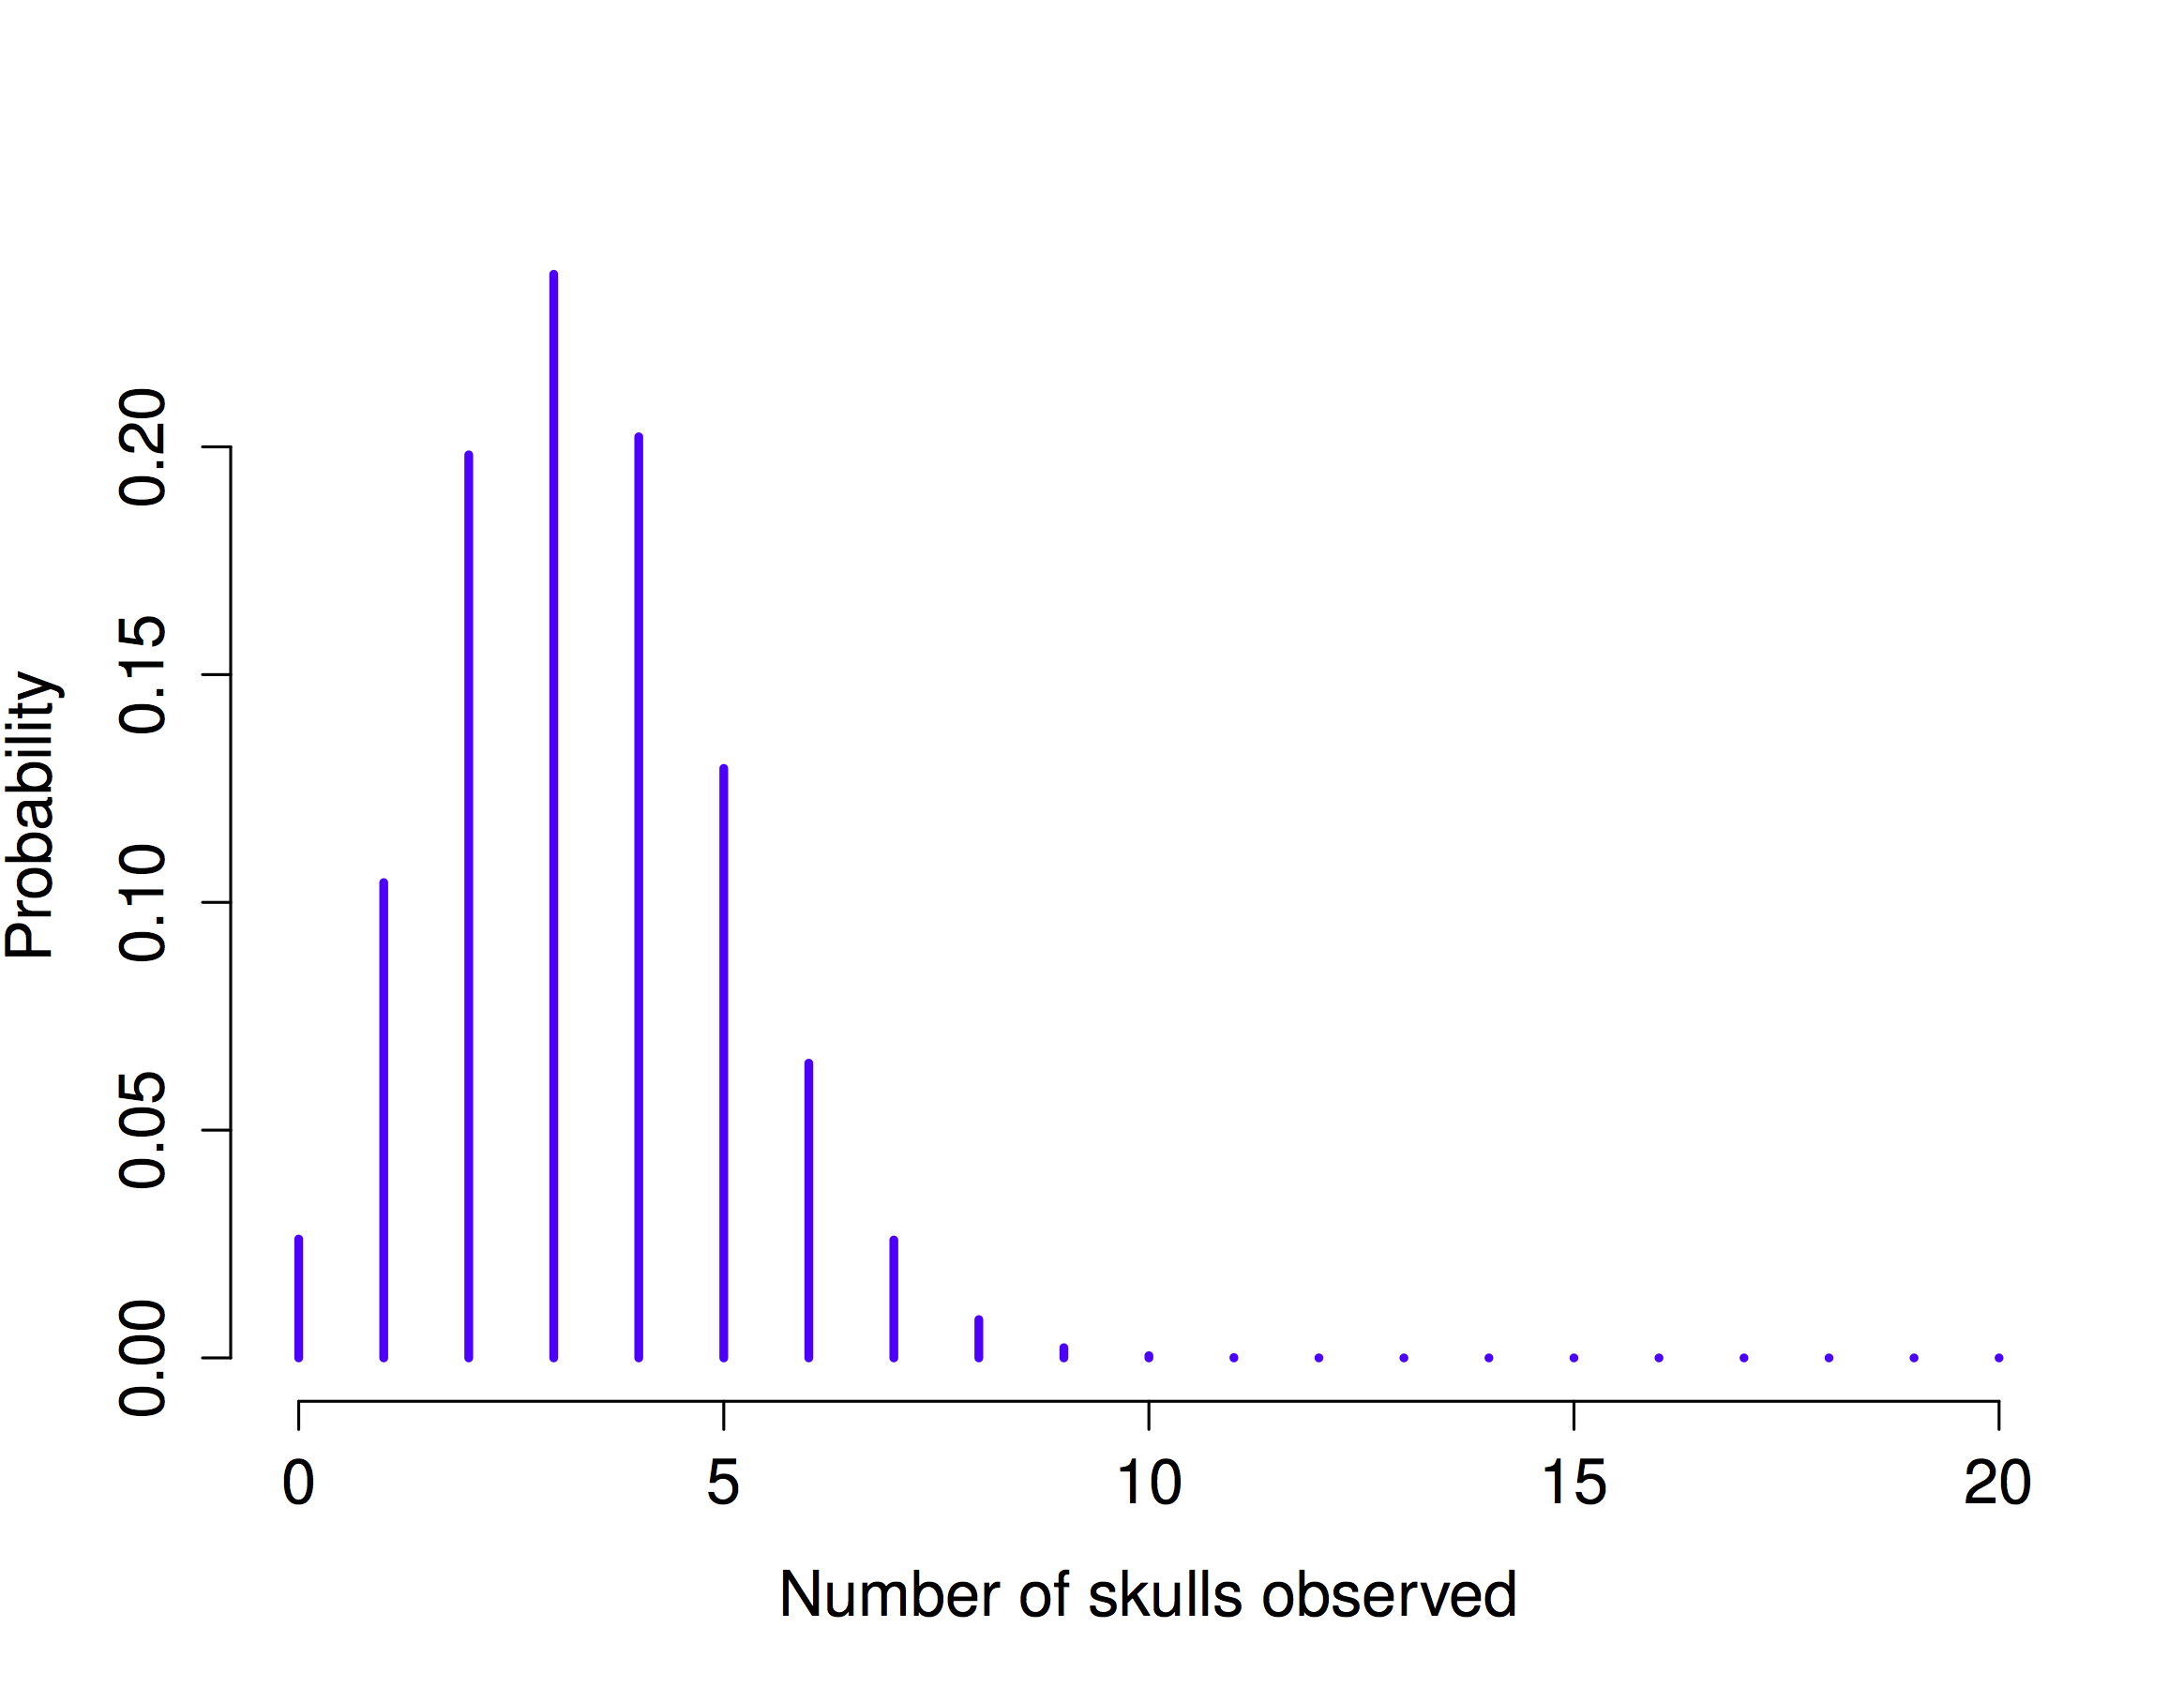
\includegraphics[width=0.75\textwidth,height=\textheight]{imgs/navarro_img/probability/binomSkulls20-eps-converted-to.png}

}

\caption{\label{fig-4binomial1}The binomial distribution with size
parameter of N =20 and an underlying success probability of 1/6. Each
vertical bar depicts the probability of one specific outcome (i.e., one
possible value of X). Because this is a probability distribution, each
of the probabilities must be a number between 0 and 1, and the heights
of the bars must sum to 1 as well.}

\end{figure}

\hypertarget{working-with-the-binomial-distribution-in-r}{%
\subsection{Working with the binomial distribution in
R}\label{working-with-the-binomial-distribution-in-r}}

R has a function called \texttt{dbinom} that calculates binomial
probabilities for us. The main arguments to the function are

\begin{itemize}
\item
  \texttt{x} This is a number, or vector of numbers, specifying the
  outcomes whose probability you're trying to calculate.
\item
  \texttt{size} This is a number telling R the size of the experiment.
\item
  \texttt{prob} This is the success probability for any one trial in the
  experiment.
\end{itemize}

So, in order to calculate the probability of getting skulls, from an
experiment of trials, in which the probability of getting a skull on any
one trial is \ldots{} well, the command I would use is simply this:

\begin{Shaded}
\begin{Highlighting}[]
\FunctionTok{dbinom}\NormalTok{( }\AttributeTok{x =} \DecValTok{4}\NormalTok{, }\AttributeTok{size =} \DecValTok{20}\NormalTok{, }\AttributeTok{prob =} \DecValTok{1}\SpecialCharTok{/}\DecValTok{6}\NormalTok{ )}
\CommentTok{\#\textgreater{} [1] 0.2022036}
\end{Highlighting}
\end{Shaded}

To give you a feel for how the binomial distribution changes when we
alter the values of \(\theta\) and \(N\), let's suppose that instead of
rolling dice, I'm actually flipping coins. This time around, my
experiment involves flipping a fair coin repeatedly, and the outcome
that I'm interested in is the number of heads that I observe. In this
scenario, the success probability is now \(\theta = 1/2\). Suppose I
were to flip the coin \(N=20\) times. In this example, I've changed the
success probability, but kept the size of the experiment the same. What
does this do to our binomial distribution?

\begin{figure}

{\centering 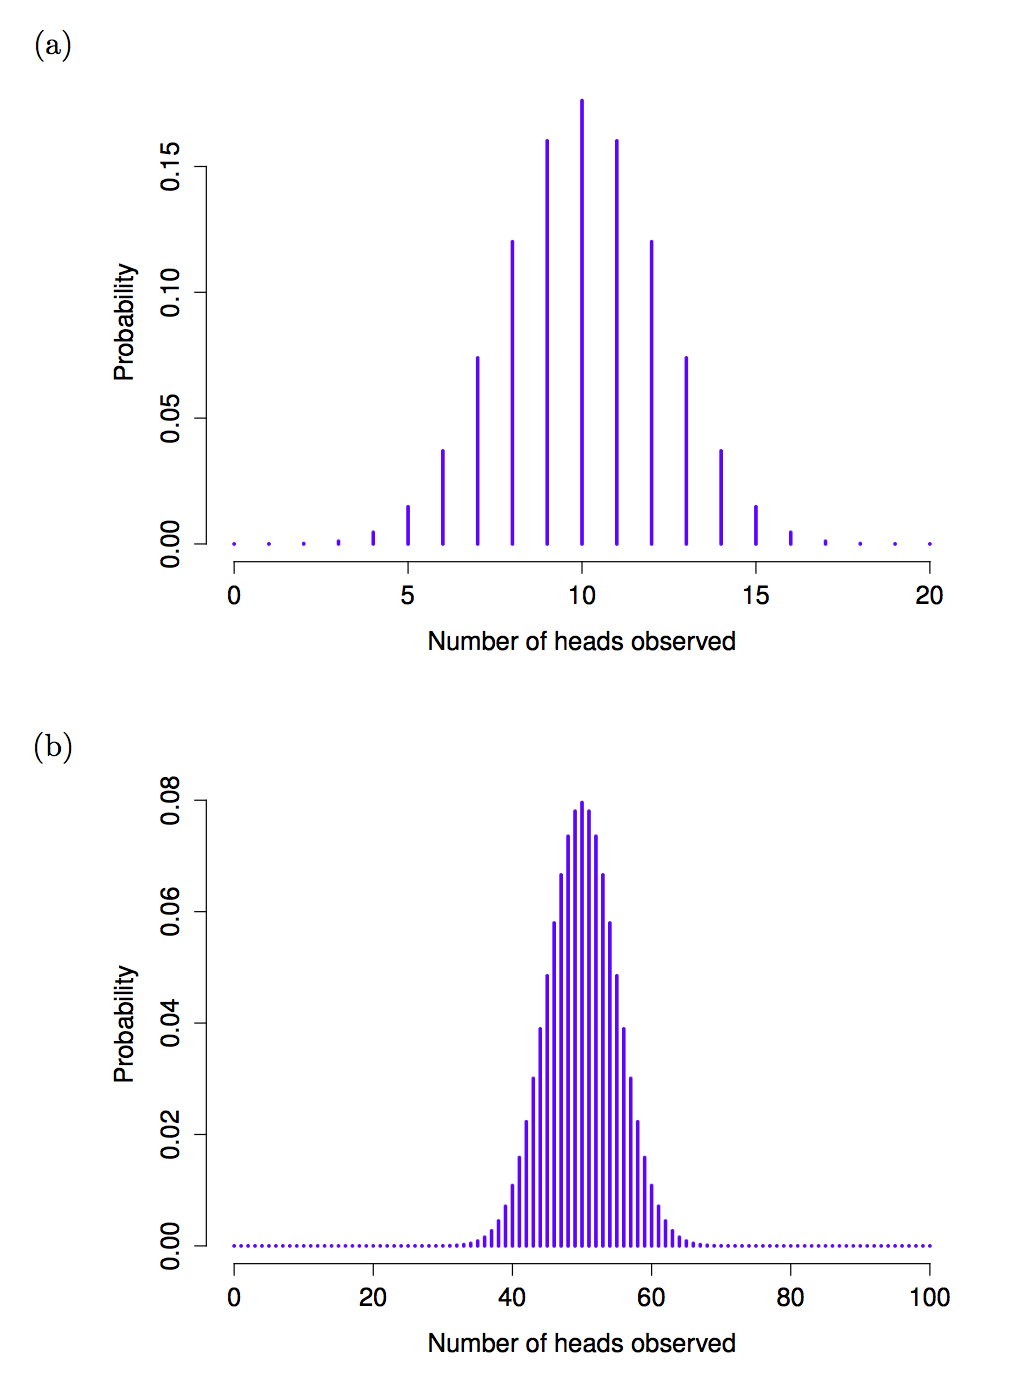
\includegraphics[width=0.75\textwidth,height=\textheight]{imgs/navarro_img/probability/Binomial2.png}

}

\caption{\label{fig-4binomial2}Two binomial distributions, involving a
scenario in which I'm flipping a fair coin, so the underlying success
probability is 1/2. In panel (a), we assume I'm flipping the coin N = 20
times. In panel (b) we assume that the coin is flipped N = 100 times.}

\end{figure}

Well, as Figure~\ref{fig-4binomial2} \(a\) shows, the main effect of
this is to shift the whole distribution, as you'd expect. Okay, what if
we flipped a coin \(N=100\) times? Well, in that case, we get
Figure~\ref{fig-4binomial2} \(b\). The distribution stays roughly in the
middle, but there's a bit more variability in the possible outcomes.

At this point, I should probably explain the name of the \texttt{dbinom}
function. Obviously, the ``binom'' part comes from the fact that we're
working with the binomial distribution, but the ``d'' prefix is probably
a bit of a mystery. In this section I'll give a partial explanation:
specifically, I'll explain why there is a prefix. As for why it's a
``d'' specifically, you'll have to wait until the next section. What's
going on here is that R actually provides \textbf{four} functions in
relation to the binomial distribution. These four functions are
\texttt{dbinom}, \texttt{pbinom}, \texttt{rbinom} and \texttt{qbinom},
and each one calculates a different quantity of interest. Not only that,
R does the same thing for \textbf{every} probability distribution that
it implements. No matter what distribution you're talking about, there's
a \texttt{d} function, a \texttt{p} function, \texttt{r} a function and
a \texttt{q} function.

Let's have a look at what all four functions do. Firstly, all four
versions of the function require you to specify the \texttt{size} and
\texttt{prob} arguments: no matter what you're trying to get R to
calculate, it needs to know what the parameters are. However, they
differ in terms of what the other argument is, and what the output is.
So let's look at them one at a time.

\begin{itemize}
\item
  The \texttt{d} form we've already seen: you specify a particular
  outcome \texttt{x}, and the output is the probability of obtaining
  exactly that outcome. (the ``d'' is short for \emph{density}, but
  ignore that for now).
\item
  The \texttt{p} form calculates the \emph{cumulative probability}. You
  specify a particular quantile \texttt{q} , and it tells you the
  probability of obtaining an outcome \textbf{smaller than or equal to}
  \texttt{q}.
\item
  The \texttt{q} form calculates the \emph{quantiles} of the
  distribution. You specify a probability value \texttt{p}, and it gives
  you the corresponding percentile. That is, the value of the variable
  for which there's a probability \texttt{p} of obtaining an outcome
  lower than that value.
\item
  The \texttt{r} form is a \emph{random number generator}: specifically,
  it generates \texttt{n} random outcomes from the distribution.
\end{itemize}

This is a little abstract, so let's look at some concrete examples.
Again, we've already covered \texttt{dbinom} so let's focus on the other
three versions. We'll start with \texttt{pbinom}, and we'll go back to
the skull-dice example. Again, I'm rolling 20 dice, and each die has a 1
in 6 chance of coming up skulls. Suppose, however, that I want to know
the probability of rolling 4 \textbf{or fewer} skulls. If I wanted to, I
could use the \texttt{dbinom} function to calculate the exact
probability of rolling 0 skulls, 1 skull, 2 skulls, 3 skulls and 4
skulls and then add these up, but there's a faster way. Instead, I can
calculate this using the \texttt{pbinom} function. Here's the command:

\begin{Shaded}
\begin{Highlighting}[]
\FunctionTok{pbinom}\NormalTok{( }\AttributeTok{q=} \DecValTok{4}\NormalTok{, }\AttributeTok{size =} \DecValTok{20}\NormalTok{, }\AttributeTok{prob =} \DecValTok{1}\SpecialCharTok{/}\DecValTok{6}\NormalTok{)}
\CommentTok{\#\textgreater{} [1] 0.7687492}
\end{Highlighting}
\end{Shaded}

In other words, there is a 76.9\% chance that I will roll 4 or fewer
skulls. Or, to put it another way, R is telling us that a value of 4 is
actually the 76.9th percentile of this binomial distribution.

Next, let's consider the \texttt{qbinom} function. Let's say I want to
calculate the 75th percentile of the binomial distribution. If we're
sticking with our skulls example, I would use the following command to
do this:

\begin{Shaded}
\begin{Highlighting}[]
\FunctionTok{qbinom}\NormalTok{( }\AttributeTok{p =} \FloatTok{0.75}\NormalTok{, }\AttributeTok{size =} \DecValTok{20}\NormalTok{, }\AttributeTok{prob =} \DecValTok{1}\SpecialCharTok{/}\DecValTok{6}\NormalTok{ )}
\CommentTok{\#\textgreater{} [1] 4}
\end{Highlighting}
\end{Shaded}

Hm. There's something odd going on here. Let's think this through. What
the \texttt{qbinom} function appears to be telling us is that the 75th
percentile of the binomial distribution is 4, even though we saw from
the function that 4 is \textbf{actually} the 76.9th percentile. And it's
definitely the \texttt{pbinom} function that is correct. I promise. The
weirdness here comes from the fact that our binomial distribution
doesn't really \textbf{have} a 75th percentile. Not really. Why not?
Well, there's a 56.7\% chance of rolling 3 or fewer skulls (you can type
\texttt{pbinom(3,\ 20,\ 1/6)} to confirm this if you want), and a 76.9\%
chance of rolling 4 or fewer skulls. So there's a sense in which the
75th percentile should lie ``in between'' 3 and 4 skulls. But that makes
no sense at all! You can't roll 20 dice and get 3.9 of them come up
skulls. This issue can be handled in different ways: you could report an
in between value (or \textbf{interpolated} value, to use the technical
name) like 3.9, you could round down (to 3) or you could round up (to
4).

The \texttt{qbinom} function rounds upwards: if you ask for a percentile
that doesn't actually exist (like the 75th in this example), R finds the
smallest value for which the the percentile rank is \textbf{at least}
what you asked for. In this case, since the ``true'' 75th percentile
(whatever that would mean) lies somewhere between 3 and 4 skulls, R
Rounds up and gives you an answer of 4. This subtlety is tedious, I
admit, but thankfully it's only an issue for discrete distributions like
the binomial. The other distributions that I'll talk about (normal,
\(t\), \(\chi^2\) and \(F\)) are all continuous, and so R can always
return an exact quantile whenever you ask for it.

Finally, we have the random number generator. To use the \texttt{rbinom}
function, you specify how many times R should ``simulate'' the
experiment using the \texttt{n} argument, and it will generate random
outcomes from the binomial distribution. So, for instance, suppose I
were to repeat my die rolling experiment 100 times. I could get R to
simulate the results of these experiments by using the following
command:

\begin{Shaded}
\begin{Highlighting}[]
\FunctionTok{rbinom}\NormalTok{( }\AttributeTok{n =} \DecValTok{100}\NormalTok{, }\AttributeTok{size =} \DecValTok{20}\NormalTok{, }\AttributeTok{prob =} \DecValTok{1}\SpecialCharTok{/}\DecValTok{6}\NormalTok{ )}
\CommentTok{\#\textgreater{}   [1] 3 4 4 1 4 4 6 2 4 0 4 2 2 3 2 3 2 2 3 3 4 3 3 4 8 4 2 4 5 2 5 4 3 3 6 0 1}
\CommentTok{\#\textgreater{}  [38] 5 5 4 1 3 3 2 4 4 1 3 4 1 1 2 2 5 2 2 3 2 2 4 2 0 6 3 3 3 2 1 2 5 5 6 7 5}
\CommentTok{\#\textgreater{}  [75] 3 3 2 5 3 3 2 6 5 2 3 1 4 3 3 4 5 2 1 4 4 3 5 2 4 3}
\end{Highlighting}
\end{Shaded}

As you can see, these numbers are pretty much what you'd expect given
the distribution shown in Figure~\ref{fig-4binomial1} . Most of the time
I roll somewhere between 1 to 5 skulls. There are a lot of subtleties
associated with random number generation using a computer, but for the
purposes of this book we don't need to worry too much about them.

\hypertarget{the-normal-distribution}{%
\section{The normal distribution}\label{the-normal-distribution}}

While the binomial distribution is conceptually the simplest
distribution to understand, it's not the most important one. That
particular honor goes to the \emph{normal distribution}, which is also
referred to as ``the bell curve'' or a ``Gaussian distribution''.

\begin{figure}

{\centering 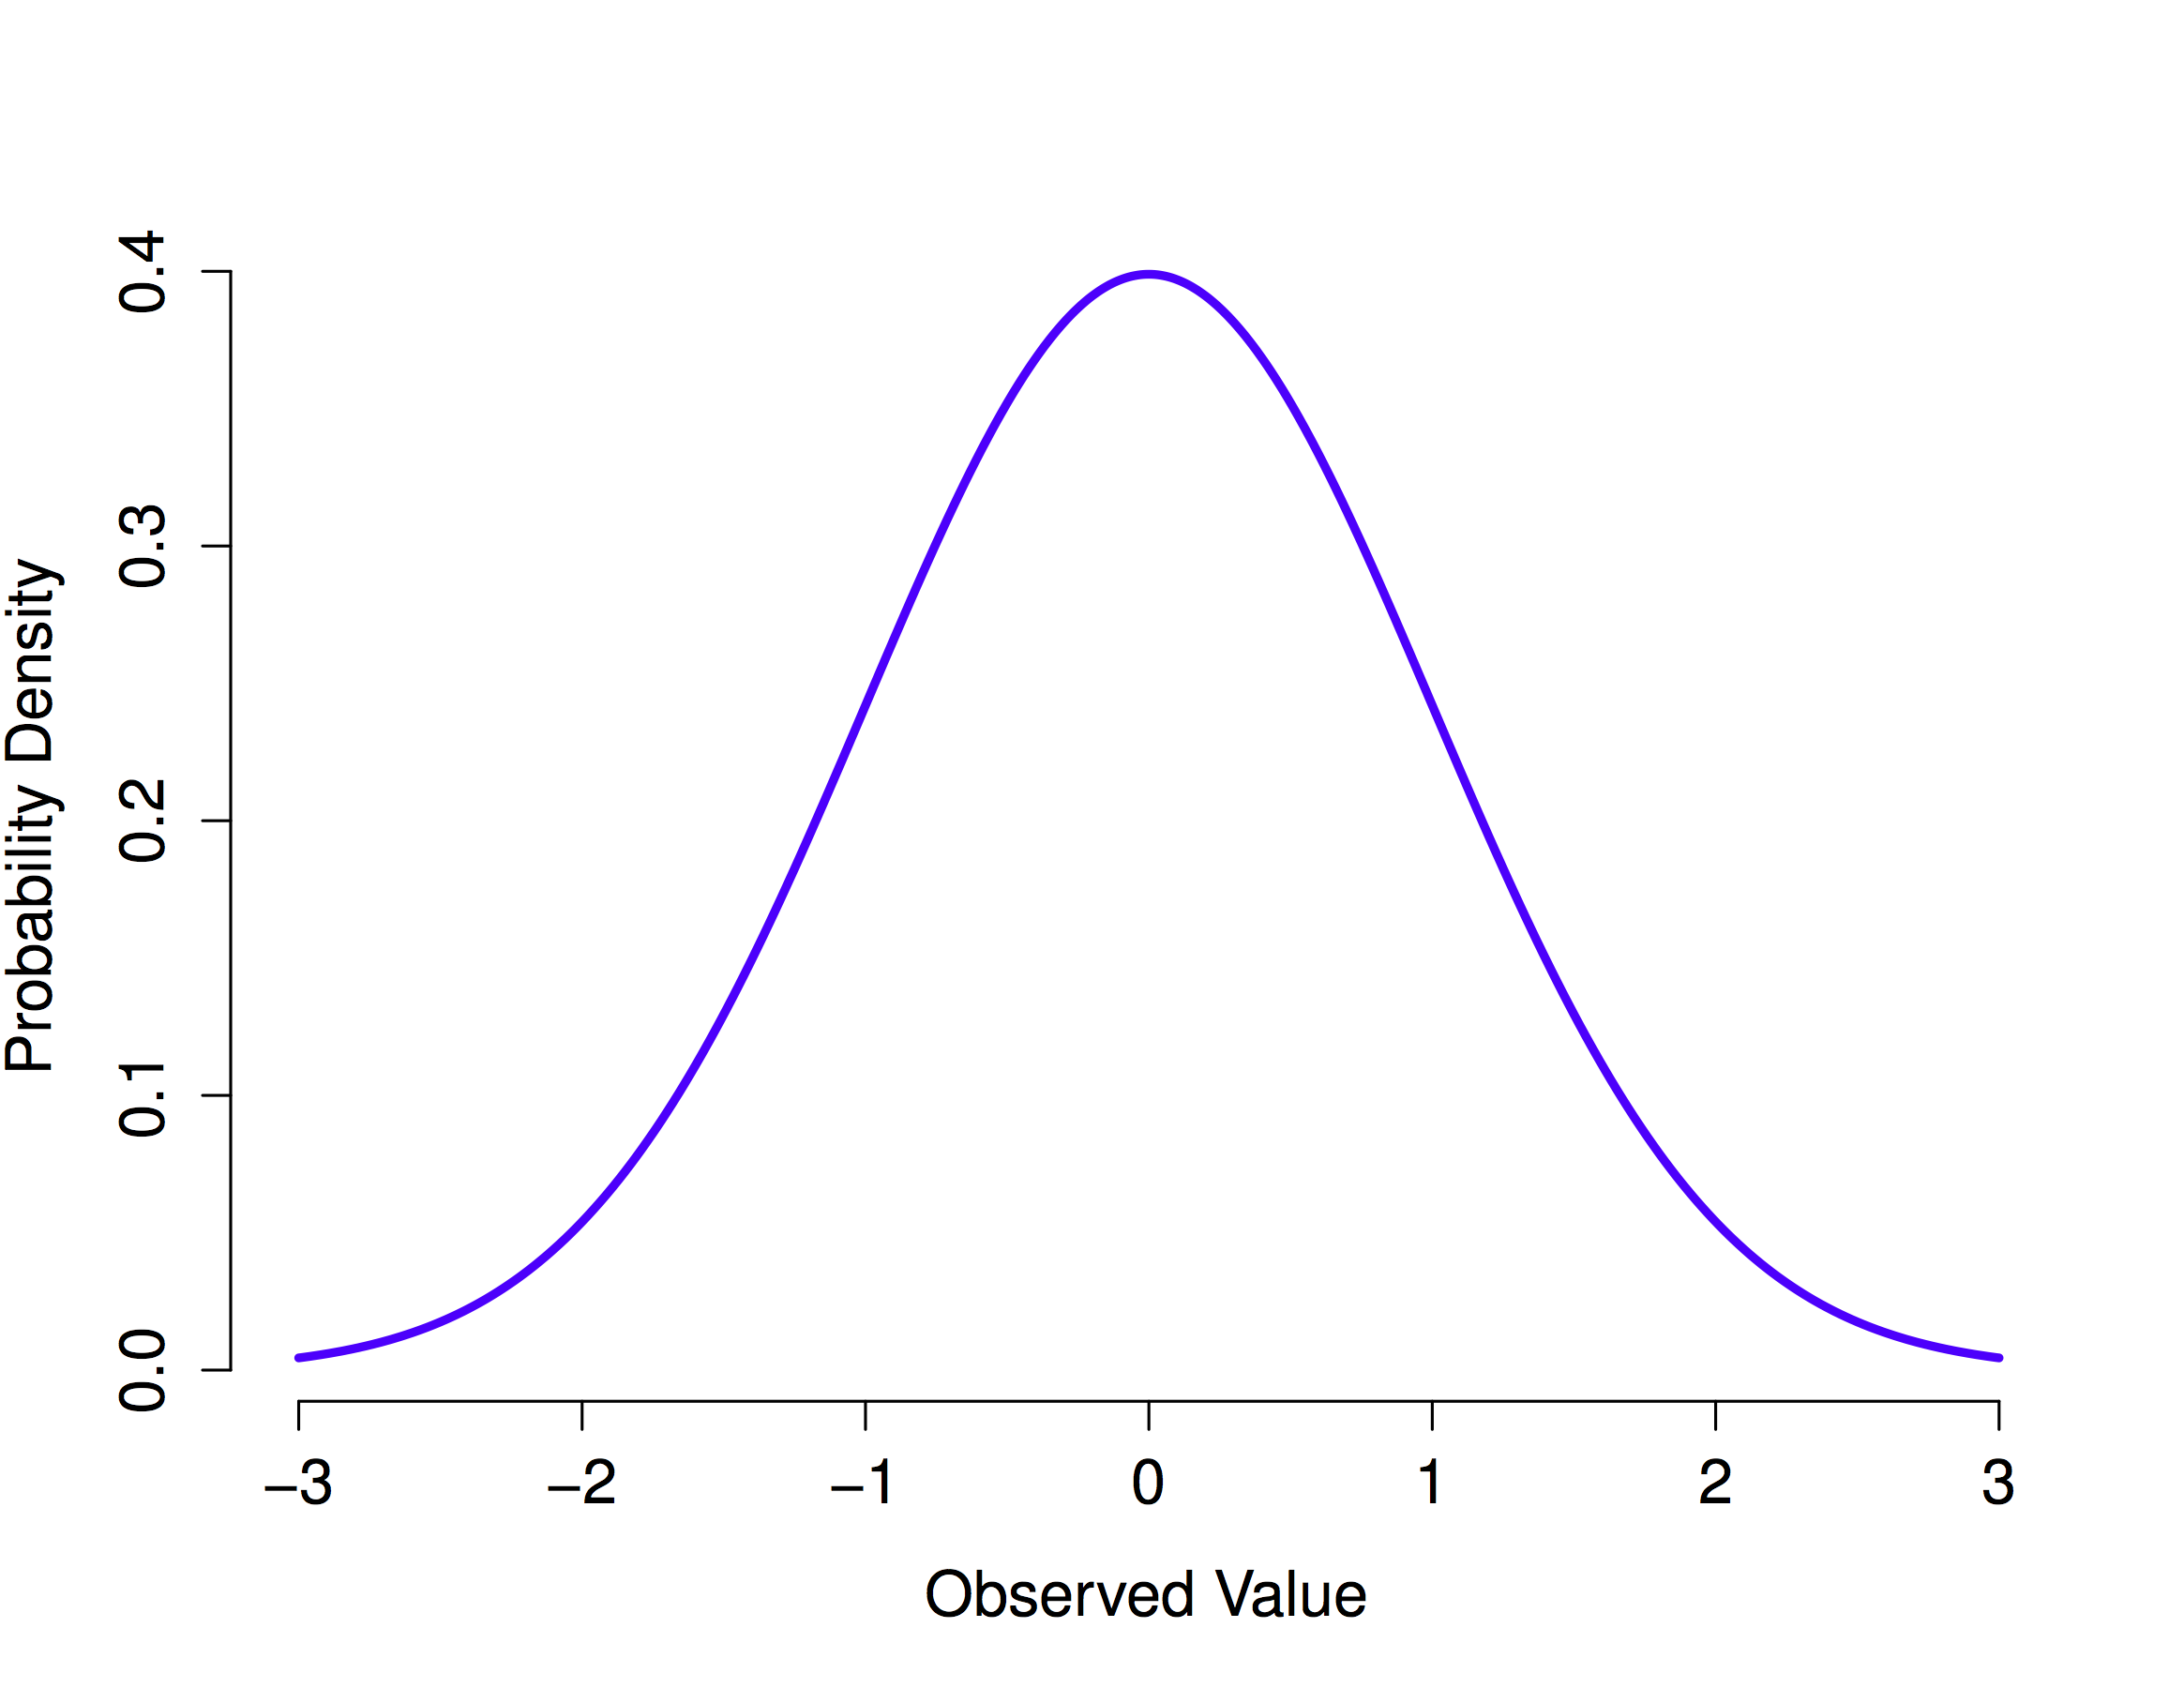
\includegraphics[width=0.75\textwidth,height=\textheight]{imgs/navarro_img/probability/standardNormal-eps-converted-to.png}

}

\caption{\label{fig-4normal}The normal distribution with mean = 0 and
standard deviation = 1. The x-axis corresponds to the value of some
variable, and the y-axis tells us something about how likely we are to
observe that value. However, notice that the y-axis is labelled
Probability Density and not Probability. There is a subtle and somewhat
frustrating characteristic of continuous distributions that makes the y
axis behave a bit oddly: the height of the curve here isn't actually the
probability of observing a particular x value. On the other hand, it is
true that the heights of the curve tells you which x values are more
likely (the higher ones!).}

\end{figure}

A normal distribution is described using two parameters, the mean of the
distribution \(\mu\) and the standard deviation of the distribution
\(\sigma\). The notation that we sometimes use to say that a variable
\(X\) is normally distributed is as follows:
\[X \sim \mbox{Normal}(\mu,\sigma)\] Of course, that's just notation. It
doesn't tell us anything interesting about the normal distribution
itself. The mathematical formula for the normal distribution is:

\begin{figure}

{\centering 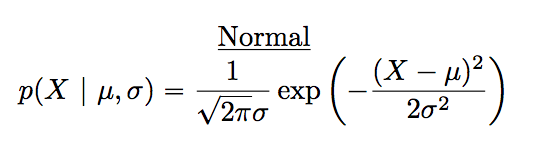
\includegraphics[width=0.75\textwidth,height=\textheight]{imgs/navarro_img/probability/Normal_formula.png}

}

\caption{Formula for the normal distribution}

\end{figure}

The formula is important enough that everyone who learns statistics
should at least look at it, but since this is an introductory text I
don't want to focus on it to much. Instead, we look at how R can be used
to work with normal distributions. The R functions for the normal
distribution are \emph{dnorm()}, \emph{pnorm()}, \emph{qnorm()} and
\emph{rnorm()}. However, they behave in pretty much exactly the same way
as the corresponding functions for the binomial distribution, so there's
not a lot that you need to know. The only thing that I should point out
is that the argument names for the parameters are \emph{mean} and
\emph{sd}. In pretty much every other respect, there's nothing else to
add.

Instead of focusing on the maths, let's try to get a sense for what it
means for a variable to be normally distributed. To that end, have a
look at Figure~\ref{fig-4normal}, which plots a normal distribution with
mean \(\mu = 0\) and standard deviation \(\sigma = 1\). You can see
where the name ``bell curve'' comes from: it looks a bit like a bell.
Notice that, unlike the plots that I drew to illustrate the binomial
distribution, the picture of the normal distribution in Figure
Figure~\ref{fig-4normal} shows a smooth curve instead of
``histogram-like'' bars. This isn't an arbitrary choice: the normal
distribution is continuous, whereas the binomial is discrete. For
instance, in the die rolling example from the last section, it was
possible to get 3 skulls or 4 skulls, but impossible to get 3.9 skulls.

With this in mind, let's see if we can get an intuition for how the
normal distribution works. First, let's have a look at what happens when
we play around with the parameters of the distribution. One parameter we
can change is the mean. This will shift the distribution to the right or
left. The animation in \textbf{?@fig-4normalMeanShift} shows a normal
distribution with mean = 0, moving up and down from mean = 0 to mean =
5. Note, when you change the mean the whole shape of the distribution
does not change, it just shifts from left to right. In the animation the
normal distribution bounces up and down a little, but that's just a
quirk of the animation (plus it looks fun that way).

In contrast, if we increase the standard deviation while keeping the
mean constant, the peak of the distribution stays in the same place, but
the distribution gets wider. The animation in
\textbf{?@fig-4normalSDShift} shows what happens when you start with a
small standard deviation (sd = 0.5), and move to larger and larger
standard deviation (up to sd = 5). As you can see, the distribution
spreads out and becomes wider as the standard deviation increases.

Notice that when we widen the distribution the height of the peak
shrinks. This has to happen: in the same way that the heights of the
bars that we used to draw a discrete binomial distribution have to
\emph{sum} to 1, the total \emph{area under the curve} for the normal
distribution must equal 1. Before moving on, I want to point out one
important characteristic of the normal distribution. Irrespective of
what the actual mean and standard deviation are, 68.3\% of the area
falls within 1 standard deviation of the mean. Similarly, 95.4\% of the
distribution falls within 2 standard deviations of the mean, and 99.7\%
of the distribution is within 3 standard deviations.

\hypertarget{probability-density}{%
\subsection{Probability density}\label{probability-density}}

There's something I've been trying to hide throughout my discussion of
the normal distribution, something that some introductory textbooks omit
completely. They might be right to do so: this ``thing'' that I'm hiding
is weird and counter intuitive even by the admittedly distorted
standards that apply in statistics. Fortunately, it's not something that
you need to understand at a deep level in order to do basic statistics:
rather, it's something that starts to become important later on when you
move beyond the basics. So, if it doesn't make complete sense, don't
worry: try to make sure that you follow the gist of it.

Throughout my discussion of the normal distribution, there's been one or
two things that don't quite make sense. Perhaps you noticed that the
\(y\)-axis in these figures is labelled ``Probability Density'' rather
than density. Maybe you noticed that I used \(p(X)\) instead of \(P(X)\)
when giving the formula for the normal distribution. Maybe you're
wondering why R uses the ``d'' prefix for functions like \emph{dnorm()}.
And maybe, just maybe, you've been playing around with the
\emph{dnorm()} function, and you accidentally typed in a command like
this:

\begin{Shaded}
\begin{Highlighting}[]
\FunctionTok{dnorm}\NormalTok{( }\AttributeTok{x =} \DecValTok{1}\NormalTok{, }\AttributeTok{mean =} \DecValTok{1}\NormalTok{, }\AttributeTok{sd =} \FloatTok{0.1}\NormalTok{ )}
\CommentTok{\#\textgreater{} [1] 3.989423}
\end{Highlighting}
\end{Shaded}

And if you've done the last part, you're probably very confused. I've
asked R to calculate the probability that \emph{x = 1}, for a normally
distributed variable with \emph{mean = 1} and standard deviation
\emph{sd = 0.1}; and it tells me that the probability is 3.99. But, as
we discussed earlier, probabilities \emph{can't} be larger than 1. So
either I've made a mistake, or that's not a probability.

As it turns out, the second answer is correct. What we've calculated
here isn't actually a probability: it's something else. To understand
what that something is, you have to spend a little time thinking about
what it really \emph{means} to say that \(X\) is a continuous variable.
Let's say we're talking about the temperature outside. The thermometer
tells me it's 23 degrees, but I know that's not really true. It's not
\emph{exactly} 23 degrees. Maybe it's 23.1 degrees, I think to myself.
But I know that that's not really true either, because it might actually
be 23.09 degrees. But, I know that\ldots{} well, you get the idea. The
tricky thing with genuinely continuous quantities is that you never
really know exactly what they are.

Now think about what this implies when we talk about probabilities.
Suppose that tomorrow's maximum temperature is sampled from a normal
distribution with mean 23 and standard deviation 1. What's the
probability that the temperature will be \emph{exactly} 23 degrees? The
answer is ``zero'', or possibly, ``a number so close to zero that it
might as well be zero''. Why is this?

It's like trying to throw a dart at an infinitely small dart board: no
matter how good your aim, you'll never hit it. In real life you'll never
get a value of exactly 23. It'll always be something like 23.1 or
22.99998 or something. In other words, it's completely meaningless to
talk about the probability that the temperature is exactly 23 degrees.
However, in everyday language, if I told you that it was 23 degrees
outside and it turned out to be 22.9998 degrees, you probably wouldn't
call me a liar. Because in everyday language, ``23 degrees'' usually
means something like ``somewhere between 22.5 and 23.5 degrees''. And
while it doesn't feel very meaningful to ask about the probability that
the temperature is exactly 23 degrees, it does seem sensible to ask
about the probability that the temperature lies between 22.5 and 23.5,
or between 20 and 30, or any other range of temperatures.

The point of this discussion is to make clear that, when we're talking
about continuous distributions, it's not meaningful to talk about the
probability of a specific value. However, what we \emph{can} talk about
is the \textbf{probability that the value lies within a particular range
of values}. To find out the probability associated with a particular
range, what you need to do is calculate the ``area under the curve''.

Okay, so that explains part of the story. I've explained a little bit
about how continuous probability distributions should be interpreted
(i.e., area under the curve is the key thing), but I haven't actually
explained what the \emph{dnorm()} function actually calculates.
Equivalently, what does the formula for \(p(x)\) that I described
earlier actually mean? Obviously, \(p(x)\) doesn't describe a
probability, but what is it? The name for this quantity \(p(x)\) is a
\emph{probability density}, and in terms of the plots we've been
drawing, it corresponds to the \emph{height} of the curve. The densities
themselves aren't meaningful in and of themselves: but they're
``rigged'' to ensure that the \emph{area} under the curve is always
interpretable as genuine probabilities. To be honest, that's about as
much as you really need to know for now.

\hypertarget{other-useful-distributions}{%
\section{Other useful distributions}\label{other-useful-distributions}}

There are many other useful distributions, these include the \texttt{t}
distribution, the \texttt{F} distribution, and the chi squared
distribution. We will soon discover more about the \texttt{t} and
\texttt{F} distributions when we discuss t-tests and ANOVAs in later
chapters.

\hypertarget{summary-of-probability}{%
\section{Summary of Probability}\label{summary-of-probability}}

We've talked what probability means, and why statisticians can't agree
on what it means. We talked about the rules that probabilities have to
obey. And we introduced the idea of a probability distribution, and
spent a good chunk talking about some of the more important probability
distributions that statisticians work with. We talked about things like
this:

\begin{itemize}
\item
  Probability theory versus statistics
\item
  Frequentist versus Bayesian views of probability
\item
  Basics of probability theory
\item
  Binomial distribution, normal distribution
\end{itemize}

As you'd expect, this coverage is by no means exhaustive. Probability
theory is a large branch of mathematics in its own right, entirely
separate from its application to statistics and data analysis. As such,
there are thousands of books written on the subject and universities
generally offer multiple classes devoted entirely to probability theory.
Even the ``simpler'' task of documenting standard probability
distributions is a big topic.Fortunately for you, very little of this is
necessary. You're unlikely to need to know dozens of statistical
distributions when you go out and do real world data analysis, and you
definitely won't need them for this book, but it never hurts to know
that there's other possibilities out there.

Picking up on that last point, there's a sense in which this whole
chapter is something of a digression. Many statistics classes skim over
this content very quickly (I know mine did), and even the more advanced
classes will often ``forget'' to revisit the basic foundations of the
field. Many academics would not know the difference between probability
and density, and until recently very few would have been aware of the
difference between Bayesian and frequentist probability. However, I
think it's important to understand these things before moving onto the
applications. For example, there are a lot of rules about what you're
``allowed'' to say when doing statistical inference, and many of these
can seem arbitrary and weird. However, they start to make sense if you
understand that there is this Bayesian/frequentist distinction.

\hypertarget{samples-populations-and-sampling}{%
\section{Samples, populations and
sampling}\label{samples-populations-and-sampling}}

Remember, the role of descriptive statistics is to concisely summarize
what we \textbf{do} know. In contrast, the purpose of inferential
statistics is to ``learn what we do not know from what we do''. What
kinds of things would we like to learn about? And how do we learn them?
These are the questions that lie at the heart of inferential statistics,
and they are traditionally divided into two ``big ideas'': estimation
and hypothesis testing. The goal in this chapter is to introduce the
first of these big ideas, estimation theory, but we'll talk about
sampling theory first because estimation theory doesn't make sense until
you understand sampling. So, this chapter divides into sampling theory,
and how to make use of sampling theory to discuss how statisticians
think about estimation. We have already done lots of sampling, so you
are already familiar with some of the big ideas.

\textbf{Sampling theory} plays a huge role in specifying the assumptions
upon which your statistical inferences rely. And in order to talk about
``making inferences'' the way statisticians think about it, we need to
be a bit more explicit about what it is that we're drawing inferences
\textbf{from} (the sample) and what it is that we're drawing inferences
\textbf{about} (the population).

In almost every situation of interest, what we have available to us as
researchers is a \textbf{sample} of data. We might have run experiment
with some number of participants; a polling company might have phoned
some number of people to ask questions about voting intentions; etc.
Regardless: the data set available to us is finite, and incomplete. We
can't possibly get every person in the world to do our experiment; a
polling company doesn't have the time or the money to ring up every
voter in the country etc. In our earlier discussion of descriptive
statistics, this sample was the only thing we were interested in. Our
only goal was to find ways of describing, summarizing and graphing that
sample. This is about to change.

\hypertarget{defining-a-population}{%
\subsection{Defining a population}\label{defining-a-population}}

A sample is a concrete thing. You can open up a data file, and there's
the data from your sample. A \textbf{population}, on the other hand, is
a more abstract idea. It refers to the set of all possible people, or
all possible observations, that you want to draw conclusions about, and
is generally \textbf{much} bigger than the sample. In an ideal world,
the researcher would begin the study with a clear idea of what the
population of interest is, since the process of designing a study and
testing hypotheses about the data that it produces does depend on the
population about which you want to make statements. However, that
doesn't always happen in practice: usually the researcher has a fairly
vague idea of what the population is and designs the study as best
he/she can on that basis.

Sometimes it's easy to state the population of interest. For instance,
in the ``polling company'' example, the population consisted of all
voters enrolled at the a time of the study -- millions of people. The
sample was a set of 1000 people who all belong to that population. In
most situations the situation is much less simple. In a typical a
psychological experiment, determining the population of interest is a
bit more complicated. Suppose I run an experiment using 100
undergraduate students as my participants. My goal, as a cognitive
scientist, is to try to learn something about how the mind works. So,
which of the following would count as ``the population'':

\begin{itemize}
\item
  All of the undergraduate psychology students at the University of
  Adelaide?
\item
  Undergraduate psychology students in general, anywhere in the world?
\item
  Australians currently living?
\item
  Australians of similar ages to my sample?
\item
  Anyone currently alive?
\item
  Any human being, past, present or future?
\item
  Any biological organism with a sufficient degree of intelligence
  operating in a terrestrial environment?
\item
  Any intelligent being?
\end{itemize}

Each of these defines a real group of mind-possessing entities, all of
which might be of interest to me as a cognitive scientist, and it's not
at all clear which one ought to be the true population of interest.

\hypertarget{simple-random-samples}{%
\subsection{Simple random samples}\label{simple-random-samples}}

Irrespective of how we define the population, the critical point is that
the sample is a subset of the population, and our goal is to use our
knowledge of the sample to draw inferences about the properties of the
population. The relationship between the two depends on the
\textbf{procedure} by which the sample was selected. This procedure is
referred to as a \textbf{sampling method}, and it is important to
understand why it matters.

To keep things simple, imagine we have a bag containing 10 chips. Each
chip has a unique letter printed on it, so we can distinguish between
the 10 chips. The chips come in two colors, black and white.

\begin{figure}

{\centering 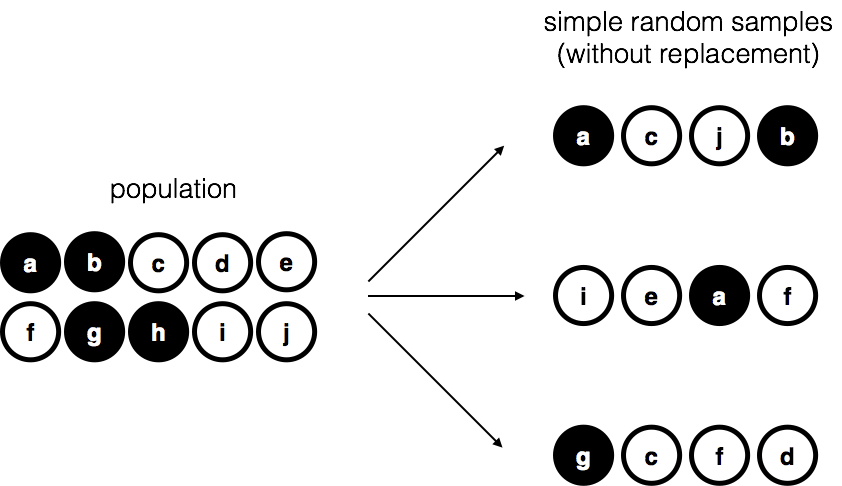
\includegraphics[width=0.75\textwidth,height=\textheight]{imgs/navarro_img/estimation/srs1.png}

}

\caption{\label{fig-srs1}Simple random sampling without replacement from
a finite population}

\end{figure}

This set of chips is the population of interest, and it is depicted
graphically on the left of Figure~\ref{fig-srs1}.

As you can see from looking at the picture, there are 4 black chips and
6 white chips, but of course in real life we wouldn't know that unless
we looked in the bag. Now imagine you run the following ``experiment'':
you shake up the bag, close your eyes, and pull out 4 chips without
putting any of them back into the bag. First out comes the \(a\) chip
(black), then the \(c\) chip (white), then \(j\) (white) and then
finally \(b\) (black). If you wanted, you could then put all the chips
back in the bag and repeat the experiment, as depicted on the right hand
side of Figure~\ref{fig-srs1}. Each time you get different results, but
the procedure is identical in each case. The fact that the same
procedure can lead to different results each time, we refer to it as a
\textbf{random} process. However, because we shook the bag before
pulling any chips out, it seems reasonable to think that every chip has
the same chance of being selected. A procedure in which every member of
the population has the same chance of being selected is called a
\textbf{simple random sample}. The fact that we did \textbf{not} put the
chips back in the bag after pulling them out means that you can't
observe the same thing twice, and in such cases the observations are
said to have been sampled \textbf{without replacement}.

To help make sure you understand the importance of the sampling
procedure, consider an alternative way in which the experiment could
have been run. Suppose that my 5-year old son had opened the bag, and
decided to pull out four black chips without putting any of them back in
the bag. This \textbf{biased} sampling scheme is depicted in
Figure~\ref{fig-brs}.

\begin{figure}

{\centering 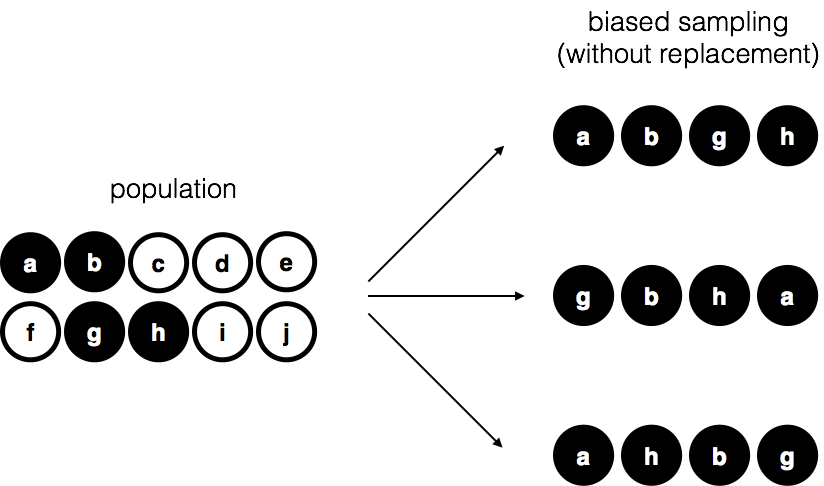
\includegraphics[width=0.75\textwidth,height=\textheight]{imgs/navarro_img/estimation/brs.png}

}

\caption{\label{fig-brs}Biased sampling without replacement from a
finite populations.}

\end{figure}

Now consider the evidentiary value of seeing 4 black chips and 0 white
chips. Clearly, it depends on the sampling scheme, does it not? If you
know that the sampling scheme is biased to select only black chips, then
a sample that consists of only black chips doesn't tell you very much
about the population! For this reason, statisticians really like it when
a data set can be considered a simple random sample, because it makes
the data analysis \textbf{much} easier.

A third procedure is worth mentioning. This time around we close our
eyes, shake the bag, and pull out a chip. This time, however, we record
the observation and then put the chip back in the bag. Again we close
our eyes, shake the bag, and pull out a chip. We then repeat this
procedure until we have 4 chips. Data sets generated in this way are
still simple random samples, but because we put the chips back in the
bag immediately after drawing them it is referred to as a sample
\textbf{with replacement}. The difference between this situation and the
first one is that it is possible to observe the same population member
multiple times, as illustrated in Figure~\ref{fig-srs2}.

\begin{figure}

{\centering 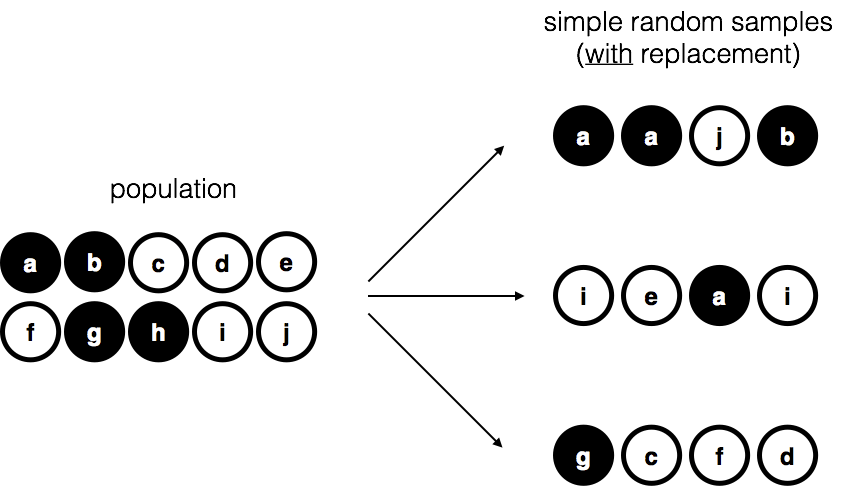
\includegraphics[width=0.75\textwidth,height=\textheight]{imgs/navarro_img/estimation/srs2.png}

}

\caption{\label{fig-srs2}Simple random sampling with replacement from a
finite population.}

\end{figure}

Most psychology experiments tend to be sampling without replacement,
because the same person is not allowed to participate in the experiment
twice. However, most statistical theory is based on the assumption that
the data arise from a simple random sample \textbf{with} replacement. In
real life, this very rarely matters. If the population of interest is
large (e.g., has more than 10 entities!) the difference between sampling
with- and without- replacement is too small to be concerned with. The
difference between simple random samples and biased samples, on the
other hand, is not such an easy thing to dismiss.

\hypertarget{most-samples-are-not-simple-random-samples}{%
\subsection{Most samples are not simple random
samples}\label{most-samples-are-not-simple-random-samples}}

As you can see from looking at the list of possible populations that I
showed above, it is almost impossible to obtain a simple random sample
from most populations of interest. When I run experiments, I'd consider
it a minor miracle if my participants turned out to be a random sampling
of the undergraduate psychology students at Adelaide university, even
though this is by far the narrowest population that I might want to
generalize to. A thorough discussion of other types of sampling schemes
is beyond the scope of this book, but to give you a sense of what's out
there I'll list a few of the more important ones:

\begin{itemize}
\item
  \textbf{Stratified sampling}. Suppose your population is (or can be)
  divided into several different sub-populations, or \textbf{strata}.
  Perhaps you're running a study at several different sites, for
  example. Instead of trying to sample randomly from the population as a
  whole, you instead try to collect a separate random sample from each
  of the strata. Stratified sampling is sometimes easier to do than
  simple random sampling, especially when the population is already
  divided into the distinct strata. It can also be more efficient that
  simple random sampling, especially when some of the sub-populations
  are rare. For instance, when studying schizophrenia it would be much
  better to divide the population into two strata (schizophrenic and
  not-schizophrenic), and then sample an equal number of people from
  each group. If you selected people randomly, you would get so few
  schizophrenic people in the sample that your study would be useless.
  This specific kind of of stratified sampling is referred to as
  \textbf{oversampling} because it makes a deliberate attempt to
  over-represent rare groups.
\item
  \textbf{Snowball sampling} is a technique that is especially useful
  when sampling from a ``hidden'' or hard to access population, and is
  especially common in social sciences. For instance, suppose the
  researchers want to conduct an opinion poll among transgender people.
  The research team might only have contact details for a few trans
  folks, so the survey starts by asking them to participate (stage 1).
  At the end of the survey, the participants are asked to provide
  contact details for other people who might want to participate. In
  stage 2, those new contacts are surveyed. The process continues until
  the researchers have sufficient data. The big advantage to snowball
  sampling is that it gets you data in situations that might otherwise
  be impossible to get any. On the statistical side, the main
  disadvantage is that the sample is highly non-random, and non-random
  in ways that are difficult to address. On the real life side, the
  disadvantage is that the procedure can be unethical if not handled
  well, because hidden populations are often hidden for a reason. I
  chose transgender people as an example here to highlight this: if you
  weren't careful you might end up outing people who don't want to be
  outed (very, very bad form), and even if you don't make that mistake
  it can still be intrusive to use people's social networks to study
  them. It's certainly very hard to get people's informed consent
  \textbf{before} contacting them, yet in many cases the simple act of
  contacting them and saying ``hey we want to study you'' can be
  hurtful. Social networks are complex things, and just because you can
  use them to get data doesn't always mean you should.
\item
  \textbf{Convenience sampling} is more or less what it sounds like. The
  samples are chosen in a way that is convenient to the researcher, and
  not selected at random from the population of interest. Snowball
  sampling is one type of convenience sampling, but there are many
  others. A common example in psychology are studies that rely on
  undergraduate psychology students. These samples are generally
  non-random in two respects: firstly, reliance on undergraduate
  psychology students automatically means that your data are restricted
  to a single sub-population. Secondly, the students usually get to pick
  which studies they participate in, so the sample is a self selected
  subset of psychology students not a randomly selected subset. In real
  life, most studies are convenience samples of one form or another.
  This is sometimes a severe limitation, but not always.
\end{itemize}

\hypertarget{how-much-does-it-matter-if-you-dont-have-a-simple-random-sample}{%
\subsection{How much does it matter if you don't have a simple random
sample?}\label{how-much-does-it-matter-if-you-dont-have-a-simple-random-sample}}

Okay, so real world data collection tends not to involve nice simple
random samples. Does that matter? A little thought should make it clear
to you that it \textbf{can} matter if your data are not a simple random
sample: just think about the difference between Figure~\ref{fig-srs1}
and Figure~\ref{fig-brs}. However, it's not quite as bad as it sounds.
Some types of biased samples are entirely unproblematic. For instance,
when using a stratified sampling technique you actually \textbf{know}
what the bias is because you created it deliberately, often to
\textbf{increase} the effectiveness of your study, and there are
statistical techniques that you can use to adjust for the biases you've
introduced (not covered in this book!). So in those situations it's not
a problem.

More generally though, it's important to remember that random sampling
is a means to an end, not the end in itself. Let's assume you've relied
on a convenience sample, and as such you can assume it's biased. A bias
in your sampling method is only a problem if it causes you to draw the
wrong conclusions. When viewed from that perspective, I'd argue that we
don't need the sample to be randomly generated in \textbf{every}
respect: we only need it to be random with respect to the
psychologically-relevant phenomenon of interest. Suppose I'm doing a
study looking at working memory capacity. In study 1, I actually have
the ability to sample randomly from all human beings currently alive,
with one exception: I can only sample people born on a Monday. In study
2, I am able to sample randomly from the Australian population. I want
to generalize my results to the population of all living humans. Which
study is better? The answer, obviously, is study 1. Why? Because we have
no reason to think that being ``born on a Monday'' has any interesting
relationship to working memory capacity. In contrast, I can think of
several reasons why ``being Australian'' might matter. Australia is a
wealthy, industrialized country with a very well-developed education
system. People growing up in that system will have had life experiences
much more similar to the experiences of the people who designed the
tests for working memory capacity. This shared experience might easily
translate into similar beliefs about how to ``take a test'', a shared
assumption about how psychological experimentation works, and so on.
These things might actually matter. For instance, ``test taking'' style
might have taught the Australian participants how to direct their
attention exclusively on fairly abstract test materials relative to
people that haven't grown up in a similar environment; leading to a
misleading picture of what working memory capacity is.

There are two points hidden in this discussion. Firstly, when designing
your own studies, it's important to think about what population you care
about, and try hard to sample in a way that is appropriate to that
population. In practice, you're usually forced to put up with a ``sample
of convenience'' (e.g., psychology lecturers sample psychology students
because that's the least expensive way to collect data, and our coffers
aren't exactly overflowing with gold), but if so you should at least
spend some time thinking about what the dangers of this practice might
be.

Secondly, if you're going to criticize someone else's study because
they've used a sample of convenience rather than laboriously sampling
randomly from the entire human population, at least have the courtesy to
offer a specific theory as to \textbf{how} this might have distorted the
results. Remember, everyone in science is aware of this issue, and does
what they can to alleviate it. Merely pointing out that ``the study only
included people from group BLAH'' is entirely unhelpful, and borders on
being insulting to the researchers, who are aware of the issue. They
just don't happen to be in possession of the infinite supply of time and
money required to construct the perfect sample. In short, if you want to
offer a responsible critique of the sampling process, then be
\textbf{helpful}. Rehashing the blindingly obvious truisms that I've
been rambling on about in this section isn't helpful.

\hypertarget{population-parameters-and-sample-statistics}{%
\subsection{Population parameters and sample
statistics}\label{population-parameters-and-sample-statistics}}

Okay. Setting aside the thorny methodological issues associated with
obtaining a random sample, let's consider a slightly different issue. Up
to this point we have been talking about populations the way a scientist
might. To a psychologist, a population might be a group of people. To an
ecologist, a population might be a group of bears. In most cases the
populations that scientists care about are concrete things that actually
exist in the real world.

Statisticians, however, are a funny lot. On the one hand, they
\textbf{are} interested in real world data and real science in the same
way that scientists are. On the other hand, they also operate in the
realm of pure abstraction in the way that mathematicians do. As a
consequence, statistical theory tends to be a bit abstract in how a
population is defined. In much the same way that psychological
researchers operationalize our abstract theoretical ideas in terms of
concrete measurements, statisticians operationalize the concept of a
``population'' in terms of mathematical objects that they know how to
work with. You've already come across these objects they're called
probability distributions (remember, the place where data comes from).

The idea is quite simple. Let's say we're talking about IQ scores. To a
psychologist, the population of interest is a group of actual humans who
have IQ scores. A statistician ``simplifies'' this by operationally
defining the population as the probability distribution depicted in
Figure~\ref{fig-IQdist} \(a\).

\begin{figure}

{\centering 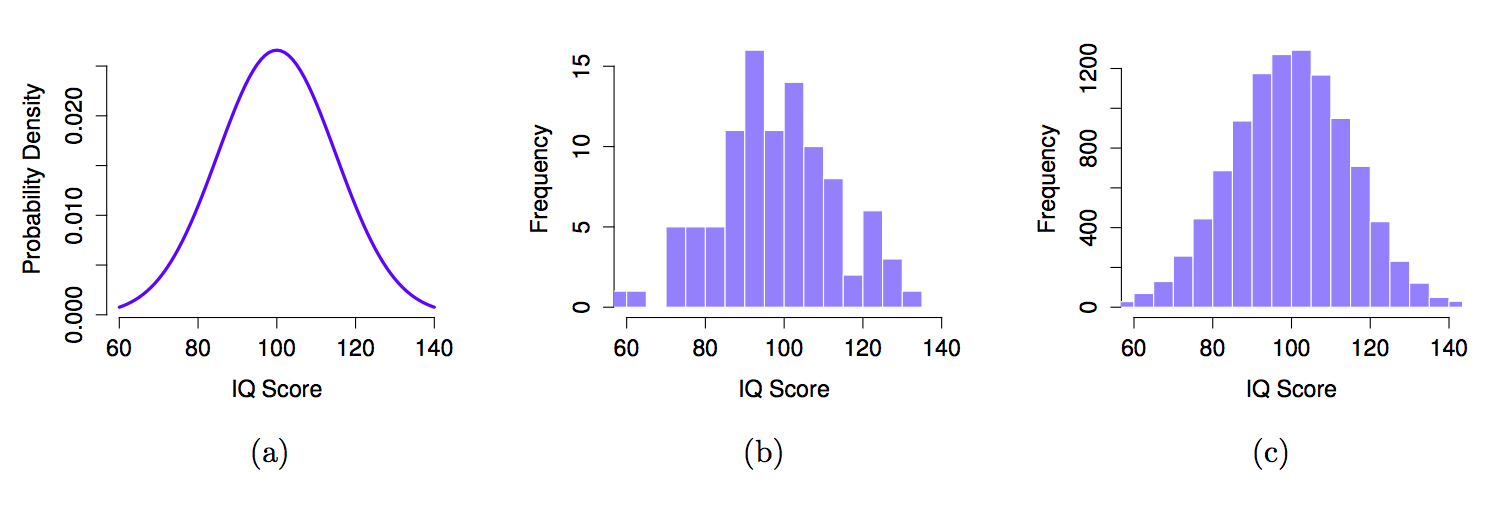
\includegraphics[width=1\textwidth,height=\textheight]{imgs/figures/navIQ.png}

}

\caption{\label{fig-IQdist}The population distribution of IQ scores
(panel a) and two samples drawn randomly from it. In panel b we have a
sample of 100 observations, and panel c we have a sample of 10,000
observations.}

\end{figure}

IQ tests are designed so that the average IQ is 100, the standard
deviation of IQ scores is 15, and the distribution of IQ scores is
normal. These values are referred to as the \textbf{population
parameters} because they are characteristics of the entire population.
That is, we say that the population mean \(\mu\) is 100, and the
population standard deviation \(\sigma\) is 15.

Now suppose we collect some data. We select 100 people at random and
administer an IQ test, giving a simple random sample from the
population. The sample would consist of a collection of numbers like
this:

\texttt{106\ 101\ 98\ 80\ 74\ ...\ 107\ 72\ 100}

Each of these IQ scores is sampled from a normal distribution with mean
100 and standard deviation 15. So if I plot a histogram of the sample, I
get something like the one shown in Figure~\ref{fig-IQdist} \(b\). As
you can see, the histogram is \textbf{roughly} the right shape, but it's
a very crude approximation to the true population distribution shown in
Figure~\ref{fig-IQdist} \(a\). The mean of the sample is fairly close to
the population mean 100 but not identical. In this case, it turns out
that the people in the sample have a mean IQ of 98.5, and the standard
deviation of their IQ scores is 15.9. These \textbf{sample statistics}
are properties of the data set, and although they are fairly similar to
the true population values, they are not the same. \textbf{In general,
sample statistics are the things you can calculate from your data set,
and the population parameters are the things you want to learn about.}
Later on in this chapter we'll talk about how you can estimate
population parameters using your sample statistics and how to work out
how confident you are in your estimates but before we get to that
there's a few more ideas in sampling theory that you need to know about.

\hypertarget{the-law-of-large-numbers}{%
\section{The law of large numbers}\label{the-law-of-large-numbers}}

We just looked at the results of one fictitious IQ experiment with a
sample size of \(N=100\). The results were somewhat encouraging: the
true population mean is 100, and the sample mean of 98.5 is a pretty
reasonable approximation to it. In many scientific studies that level of
precision is perfectly acceptable, but in other situations you need to
be a lot more precise. If we want our sample statistics to be much
closer to the population parameters, what can we do about it?

The obvious answer is to collect more data. Suppose that we ran a much
larger experiment, this time measuring the IQ's of 10,000 people. We can
simulate the results of this experiment using R, using the
\textbf{rnorm()} function, which generates random numbers sampled from a
normal distribution. For an experiment with a sample size of \textbf{n =
10000}, and a population with \textbf{mean = 100} and \textbf{sd = 15},
R produces our fake IQ data using these commands:

\begin{Shaded}
\begin{Highlighting}[]
\NormalTok{IQ }\OtherTok{\textless{}{-}} \FunctionTok{rnorm}\NormalTok{(}\AttributeTok{n=}\DecValTok{10000}\NormalTok{, }\AttributeTok{mean=}\DecValTok{100}\NormalTok{, }\AttributeTok{sd=}\DecValTok{15}\NormalTok{) }\CommentTok{\#generate IQ scores}
\NormalTok{IQ }\OtherTok{\textless{}{-}} \FunctionTok{round}\NormalTok{(IQ) }\CommentTok{\# make round numbers}
\end{Highlighting}
\end{Shaded}

Cool, we just generated 10,000 fake IQ scores. Where did they go? Well,
they went into the variable IQ on my computer. You can do the same on
your computer too by copying the above code. 10,000 numbers is too many
numbers to look at. We can look at the first 100 like this:

\begin{Shaded}
\begin{Highlighting}[]
\FunctionTok{print}\NormalTok{(IQ[}\DecValTok{1}\SpecialCharTok{:}\DecValTok{100}\NormalTok{])}
\CommentTok{\#\textgreater{}   [1]  81  96 114  96 115 114 147  81  74  97  91  89 101 101 116  87 115 131}
\CommentTok{\#\textgreater{}  [19]  78  98  73  91  87  93 102  76  82  97  97 127 105  98  95  75 101 109}
\CommentTok{\#\textgreater{}  [37]  81 123  96 124  81  92  95  86  97  80  92  97  97  86 139  88 117 114}
\CommentTok{\#\textgreater{}  [55] 105 131 101 111 103 107  84  82  91  89  99  91  79  90  75  89 103 110}
\CommentTok{\#\textgreater{}  [73] 109 111  90  95 132  75 119 104 102 106 105  87 112  83  71 102 113 114}
\CommentTok{\#\textgreater{}  [91] 113  97  88  80  89  76  85 107  86 124}
\end{Highlighting}
\end{Shaded}

We can compute the mean IQ using the command \textbf{mean(IQ)} and the
standard deviation using the command \textbf{sd(IQ)}, and draw a
histogram using \textbf{hist()}. The histogram of this much larger
sample is shown in Figure @ref(fig:IQdist)c.~Even a moment's inspections
makes clear that the larger sample is a much better approximation to the
true population distribution than the smaller one. This is reflected in
the sample statistics: the mean IQ for the larger sample turns out to be
99.9, and the standard deviation is 15.1. These values are now very
close to the true population.

I feel a bit silly saying this, but the thing I want you to take away
from this is that large samples generally give you better information. I
feel silly saying it because it's so bloody obvious that it shouldn't
need to be said. In fact, it's such an obvious point that when Jacob
Bernoulli -- one of the founders of probability theory -- formalized
this idea back in 1713, he was kind of a jerk about it. Here's how he
described the fact that we all share this intuition:

\begin{quote}
\textbf{For even the most stupid of men, by some instinct of nature, by
himself and without any instruction (which is a remarkable thing), is
convinced that the more observations have been made, the less danger
there is of wandering from one's goal} (see Stigler, 1986, p65).
\end{quote}

Okay, so the passage comes across as a bit condescending (not to mention
sexist), but his main point is correct: it really does feel obvious that
more data will give you better answers. The question is, why is this so?
Not surprisingly, this intuition that we all share turns out to be
correct, and statisticians refer to it as the \textbf{law of large
numbers}. The law of large numbers is a mathematical law that applies to
many different sample statistics, but the simplest way to think about it
is as a law about averages. The sample mean is the most obvious example
of a statistic that relies on averaging (because that's what the mean
is\ldots{} an average), so let's look at that. \textbf{When applied to
the sample mean, what the law of large numbers states is that as the
sample gets larger, the sample mean tends to get closer to the true
population mean.} Or, to say it a little bit more precisely, as the
sample size ``approaches'' infinity (written as
\(N \rightarrow \infty\)) the sample mean approaches the population mean
(\(\bar{X} \rightarrow \mu\)).

I don't intend to subject you to a proof that the law of large numbers
is true, but it's one of the most important tools for statistical
theory. The law of large numbers is the thing we can use to justify our
belief that collecting more and more data will eventually lead us to the
truth. For any particular data set, the sample statistics that we
calculate from it will be wrong, but the law of large numbers tells us
that if we keep collecting more data those sample statistics will tend
to get closer and closer to the true population parameters.

\hypertarget{sampling-distributions-and-the-central-limit-theorem}{%
\section{Sampling distributions and the central limit
theorem}\label{sampling-distributions-and-the-central-limit-theorem}}

The law of large numbers is a very powerful tool, but it's not going to
be good enough to answer all our questions. Among other things, all it
gives us is a ``long run guarantee''. In the long run, if we were
somehow able to collect an infinite amount of data, then the law of
large numbers guarantees that our sample statistics will be correct. But
as John Maynard Keynes famously argued in economics, a long run
guarantee is of little use in real life:

\begin{quote}
{[}**The{]} long run is a misleading guide to current affairs. In the
long run we are all dead. Economists set themselves too easy, too
useless a task, if in tempestuous seasons they can only tell us, that
when the storm is long past, the ocean is flat again.** Keynes (1923,
80)
\end{quote}

As in economics, so too in psychology and statistics. It is not enough
to know that we will \textbf{eventually} arrive at the right answer when
calculating the sample mean. Knowing that an infinitely large data set
will tell me the exact value of the population mean is cold comfort when
my \textbf{actual} data set has a sample size of \(N=100\). In real
life, then, we must know something about the behavior of the sample mean
when it is calculated from a more modest data set!

\hypertarget{sampling-distribution-of-the-sample-means}{%
\subsection{Sampling distribution of the sample
means}\label{sampling-distribution-of-the-sample-means}}

``Oh no, what is the sample distribution of the sample means? Is that
even allowed in English?''. Yes, unfortunately, this is allowed. The
\textbf{sampling distribution of the sample means} is the next most
important thing you will need to understand. IT IS SO IMPORTANT THAT IT
IS NECESSARY TO USE ALL CAPS. It is only confusing at first because it's
long and uses sampling and sample in the same phrase.

Don't worry, we've been prepping you for this. You know what a
distribution is right? It's where numbers comes from. It makes some
numbers occur more or less frequently, or the same as other numbers. You
know what a sample is right? It's the numbers we take from a
distribution. So, what could the sampling distribution of the sample
means refer to?

First, what do you think the sample means refers to? Well, if you took a
sample of numbers, you would have a bunch of numbers\ldots then, you
could compute the mean of those numbers. The sample mean is the mean of
the numbers in the sample. That is all. So, what is this distribution
you speak of? Well, what if you took a bunch of samples, put one here,
put one there, put some other ones other places. You have a lot of
different samples of numbers. You could compute the mean for each them.
Then you would have a bunch of means. What do those means look like?
Well, if you put them in a histogram, you could find out. If you did
that, you would be looking at (roughly) a distribution, AKA \textbf{the
sampling distribution of the sample means}.

``I'm following along sort of, why would I want to do this instead of
watching Netflix\ldots{}''. Because, the sampling distribution of the
sample means gives you another window into chance. A very useful one
that you can control, just like your remote control, by pressing the
right design buttons.

\hypertarget{seeing-the-pieces}{%
\subsection{Seeing the pieces}\label{seeing-the-pieces}}

To make a sampling distribution of the sample means, we just need the
following:

\begin{enumerate}
\def\labelenumi{\arabic{enumi}.}
\tightlist
\item
  A distribution to take numbers from
\item
  A bunch of different samples from the distribution
\item
  The means of each of the samples
\item
  Get all of the sample means, and plot them in a histogram
\end{enumerate}

\begin{center}\rule{0.5\linewidth}{0.5pt}\end{center}

Question for yourself: What do you think the sampling distribution of
the sample means will look like? Will it tend to look the shape of the
distribution that the samples came from? Or not? Good question, think
about it.

\begin{center}\rule{0.5\linewidth}{0.5pt}\end{center}

Let's do those four things. We will sample numbers from the uniform
distribution. Figure~\ref{fig-4Unif} shows the uniform distribution for
sampling the set of integers from 1 to 10:

\begin{figure}

{\centering 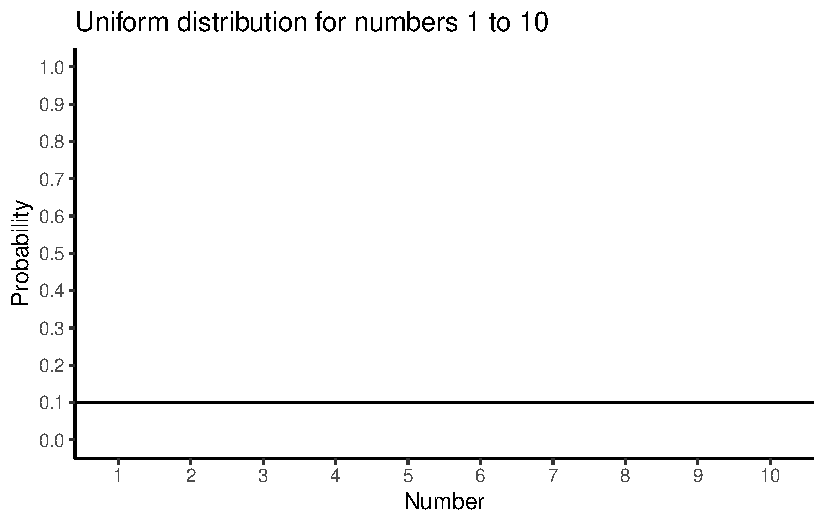
\includegraphics[width=0.75\textwidth,height=\textheight]{04-SamplesPopulations_files/figure-pdf/fig-4Unif-1.pdf}

}

\caption{\label{fig-4Unif}A uniform distribution illustrating the
probabilites of sampling the numbers 1 to 10. In a uniform distribution,
all numbers have an equal probability of being sampled, so the line is
flat indicating all numbers have the same probability}

\end{figure}

\textbf{?@fig-4sample20unif} animates the process of taking a bunch of
samples from the uniform distribution. We will set our sample-size to
20. It's easier to see how the sample mean behaves in a movie. Each
histogram shows a new sample. The red line shows where the mean of the
sample is. The samples are all very different from each other, but the
red line doesn't move around very much, it always stays near the middle.
However, the red line does move around a little bit, and this variance
is what we call the sampling distribution of the sample mean.

OK, what have we got here? We have an animation of 10 different samples.
Each sample has 20 observations and these are summarized in each of
histograms that show up in the animation. Each histogram has a red line.
The red line shows you where the mean of each sample is located. So, we
have found the sample means for the 10 different samples from a uniform
distribution.

First question. Are the sample means all the same? The answer is no.
They are all kind of similar to each other though, they are all around
five plus or minus a few numbers. This is interesting. Although all of
our samples look pretty different from one another, the means of our
samples look more similar than different.

Second question. What should we do with the means of our samples? Well,
how about we collect them them all, and then plot a histogram of them.
This would allow us to see what the distribution of the sample means
looks like. The next histogram is just this. Except, rather than taking
10 samples, we will take 10,000 samples. For each of them we will
compute the means. So, we will have 10,000 means.
Figure~\ref{fig-4unifmany} shows the histogram of the sample means:

\begin{figure}

{\centering 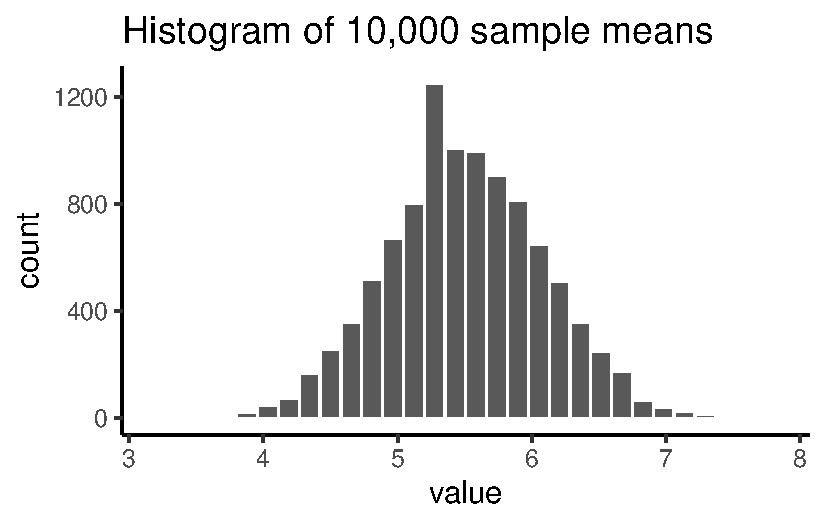
\includegraphics[width=0.75\textwidth,height=\textheight]{04-SamplesPopulations_files/figure-pdf/fig-4unifmany-1.pdf}

}

\caption{\label{fig-4unifmany}A histogram showing the sample means for
10,000 samples, each size 20, from the uniform distribution of numbers
from 1 to 10. The expected mean is 5.5, and the histogram is centered on
5.5. The mean of each sample is not always 5.5 because of sampling error
or chance}

\end{figure}

``Wait what? This doesn't look right. I thought we were taking samples
from a uniform distribution. Uniform distributions are flat. THIS DOES
NOT LOOK LIKE A FLAT DISTRIBTUION, WHAT IS GOING ON, AAAAAGGGHH.''. We
feel your pain.

Remember, we are looking at the distribution of sample means. It is
indeed true that the distribution of sample means does not look the same
as the distribution we took the samples from. Our distribution of sample
means goes up and down. In fact, this will almost always be the case for
distributions of sample means. This fact is called the \textbf{central
limit theorem}, which we talk about later.

For now, let's talk about about what's happening. Remember, we have been
sampling numbers between the range 1 to 10. We are supposed to get each
number with roughly equal frequency, because we are sampling from a
uniform distribution. So, let's say we took a sample of 10 numbers, and
happened to get one of each from 1 to 10.

\texttt{1\ 2\ 3\ 4\ 5\ 6\ 7\ 8\ 9\ 10}

What is the mean of those numbers? Well, its 1+2+3+4+5+6+7+8+9+10 = 55 /
10 = 5.5. Imagine if we took a bigger sample, say of 20 numbers, and
again we got exactly 2 of each number. What would the mean be? It would
be (1+2+3+4+5+6+7+8+9+10)*2 = 110 / 20 = 5.5. Still 5.5. You can see
here, that the mean value of our uniform distribution is 5.5. Now that
we know this, we might expect that most of our samples will have a mean
near this number. We already know that every sample won't be perfect,
and it won't have exactly an equal amount of every number. So, we will
expect the mean of our samples to vary a little bit. The histogram that
we made shows the variation. Not surprisingly, the numbers vary around
the value 5.5.

\hypertarget{sampling-distributions-exist-for-any-sample-statistic}{%
\subsection{Sampling distributions exist for any sample
statistic!}\label{sampling-distributions-exist-for-any-sample-statistic}}

One thing to keep in mind when thinking about sampling distributions is
that \textbf{any} sample statistic you might care to calculate has a
sampling distribution. For example, suppose that each time you sampled
some numbers from an experiment you wrote down the largest number in the
experiment. Doing this over and over again would give you a very
different sampling distribution, namely the \textbf{sampling
distribution of the maximum}. You could calculate the smallest number,
or the mode, or the median, of the variance, or the standard deviation,
or anything else from your sample. Then, you could repeat many times,
and produce the sampling distribution of those statistics. Neat!

Just for fun here are some different sampling distributions for
different statistics. We will take a normal distribution with mean =
100, and standard deviation =20. Then, we'll take lots of samples with n
= 50 (50 observations per sample). We'll save all of the sample
statistics, then plot their histograms in Figure~\ref{fig-4samplestats}.
Let's do it:

\begin{figure}

{\centering 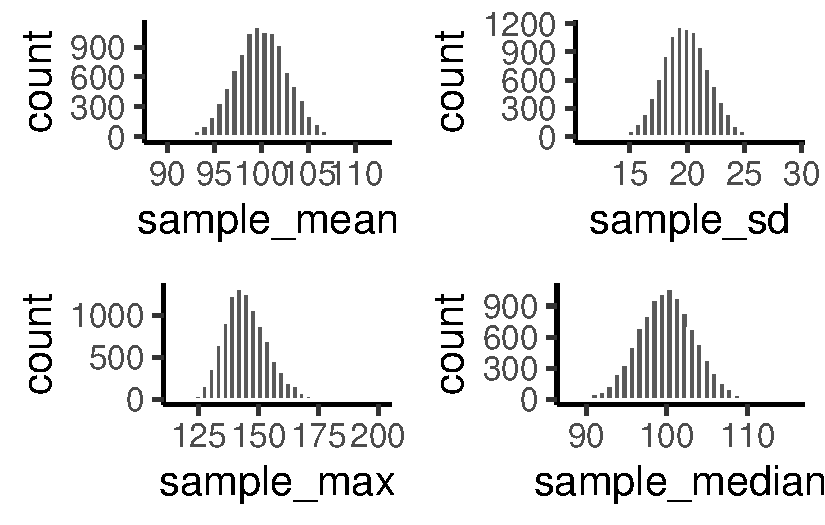
\includegraphics[width=1\textwidth,height=\textheight]{04-SamplesPopulations_files/figure-pdf/fig-4samplestats-1.pdf}

}

\caption{\label{fig-4samplestats}Each panel shows a histogram of a
different sampling statistic}

\end{figure}

We just computed 4 different sampling distributions, for the mean,
standard deviation, maximum value, and the median. If you just look
quickly at these histograms you might think they all basically look the
same. Hold up now. It's very important to look at the x-axes. They are
different. For example, the sample mean goes from about 90 to 110,
whereas the standard deviation goes from 15 to 25.

These sampling distributions are super important, and worth thinking
about. What should you think about? Well, here's a clue. These
distributions are telling you what to expect from your sample.
Critically, they are telling you what you should expect from a sample,
when you take one from the specific distribution that we used (normal
distribution with mean =100 and SD = 20). What have we learned. We've
learned a tonne. We've learned that we can expect our sample to have a
mean somewhere between 90 and 108ish. Notice, the sample means are never
more extreme. We've learned that our sample will usually have some
variance, and that the the standard deviation will be somewhere between
15 and 25 (never much more extreme than that). We can see that sometime
we get some big numbers, say between 120 and 180, but not much bigger
than that. And, we can see that the median is pretty similar to the
mean. If you ever took a sample of 50 numbers, and your descriptive
statistics were inside these windows, then perhaps they came from this
kind of normal distribution. If your sample statistics are very
different, then your sample probably did not come this distribution. By
using simulation, we can find out what samples look like when they come
from distributions, and we can use this information to make inferences
about whether our sample came from particular distributions.

\hypertarget{the-central-limit-theorem}{%
\section{The central limit theorem}\label{the-central-limit-theorem}}

OK, so now you've seen lots of sampling distributions, and you know what
the sampling distribution of the mean is. Here, we'll focus on
\textbf{how the sampling distribution of the mean changes as a function
of sample size.}

Intuitively, you already know part of the answer: if you only have a few
observations, the sample mean is likely to be quite inaccurate (you've
already seen it bounce around): if you replicate a small experiment and
recalculate the mean you'll get a very different answer. In other words,
the sampling distribution is quite wide. If you replicate a large
experiment and recalculate the sample mean you'll probably get the same
answer you got last time, so the sampling distribution will be very
narrow.

Let's give ourselves a nice movie to see everything in action. We're
going to sample numbers from a normal distribution.
\textbf{?@fig-4samplingmean} has four panels, each panel represents a
different sample size (n), including sample-sizes of 10, 50, 100, and
1000. The red line shows the shape of the normal distribution. The grey
bars show a histogram of each of the samples that we take. The red line
shows the mean of an individual sample (the middle of the grey bars). As
you can see, the red line moves around a lot, especially when the sample
size is small (10).

The new bits are the blue bars and the blue lines. The blue bars
represent the sampling distribution of the sample mean. For example, in
the panel for sample-size 10, we see a bunch of blue bars. This is a
histogram of 10 sample means, taken from 10 samples of size 10. In the
50 panel, we see a histogram of 50 sample means, taken from 50 samples
of size 50, and so on. The blue line in each panel is the mean of the
sample means (``aaagh, it's a mean of means'', yes it is).

What should you notice? Notice that the range of the blue bars shrinks
as sample size increases. The sampling distribution of the mean is quite
wide when the sample-size is 10, it narrows as sample-size increases to
50 and 100, and it's just one bar, right in the middle when sample-size
goes to 1000. What we are seeing is that the mean of the sampling
distribution approaches the mean of the population as sample-size
increases.

So, the sampling distribution of the mean is another distribution, and
it has some variance. It varies more when sample-size is small, and
varies less when sample-size is large. We can quantify this effect by
calculating the standard deviation of the sampling distribution, which
is referred to as the \textbf{standard error}. The standard error of a
statistic is often denoted SE, and since we're usually interested in the
standard error of the sample \textbf{mean}, we often use the acronym
SEM. As you can see just by looking at the movie, as the sample size
\(N\) increases, the SEM decreases.

Okay, so that's one part of the story. However, there's something we've
been glossing over a little bit. We've seen it already, but it's worth
looking at it one more time. Here's the thing: \textbf{no matter what
shape your population distribution is}, as \(N\) increases the sampling
distribution of the mean starts to look more like a normal distribution.
This is the central limit theorem.

To see the central limit theorem in action, we are going to look at some
histograms of sample means from different kinds of distributions. It is
very important to recognize that you are looking at distributions of
sample means, not distributions of individual samples.

Here we go, Figure~\ref{fig-4sampledistmeannorm} shows sampling from a
normal distribution. The red line is the normal distribution where each
sample is drawn from. The mean for each sample of numbers is computed,
and the distribution of sample means is shown by the blue bars. Note
that the shape of red line and the blue bars are similar, they both look
like a normal distribution.

\begin{figure}

{\centering 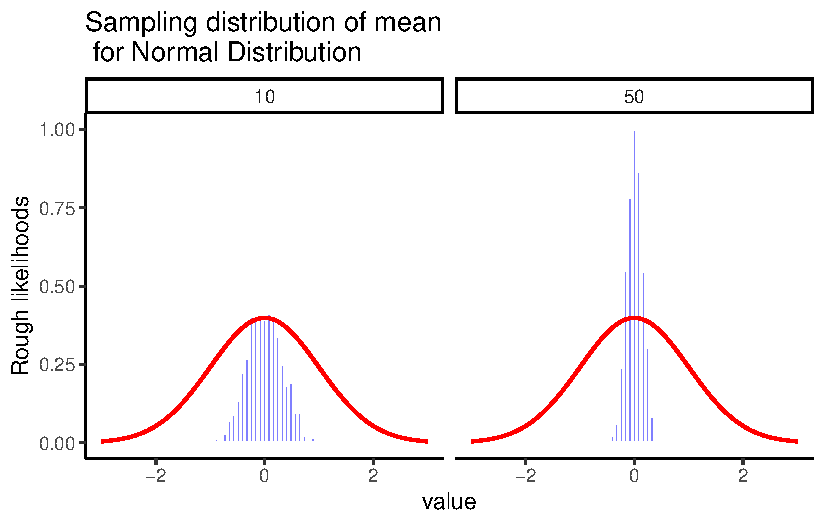
\includegraphics[width=0.75\textwidth,height=\textheight]{04-SamplesPopulations_files/figure-pdf/fig-4sampledistmeannorm-1.pdf}

}

\caption{\label{fig-4sampledistmeannorm}Comparison of two normal
distributions, and histograms for the sampling distribution of the mean
for different samples-sizes. The range of sampling distribution of the
mean shrinks as sample-size increases}

\end{figure}

Let's do it again. This time we will sample from a flat uniform
distribution shown by the red line. However,
Figure~\ref{fig-4samplemeanunif} shows the distribution of sample means
represented by the blue bars is not flat, it looks like a normal
distribution.

\begin{figure}

{\centering 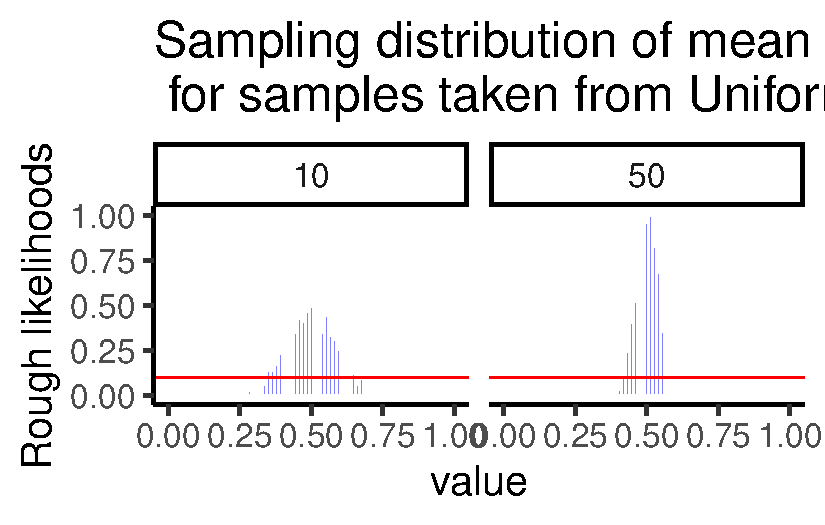
\includegraphics[width=1\textwidth,height=\textheight]{04-SamplesPopulations_files/figure-pdf/fig-4samplemeanunif-1.pdf}

}

\caption{\label{fig-4samplemeanunif}Illustration that the shape of the
sampling distribution of the mean is normal, even when the samples come
from a non-normal (uniform in this case) distribution}

\end{figure}

One more time with an exponential distribution (shown in red) where
smaller numbers are more likely to be sampled than larger numbers. Even
though way more of the numbers in a given sample will be smaller than
larger, according to Figure~\ref{fig-4samplemeanExp} the sampling
distribution of the mean does not look the red line. Instead, the
sampling distribution of the mean looks like a bell-shaped normal curve.
This is the central limit theorem in action.

\begin{figure}

{\centering 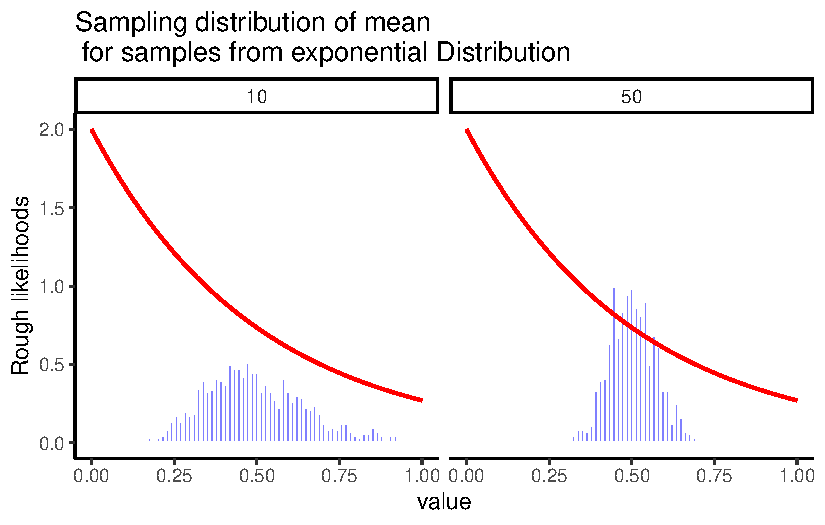
\includegraphics[width=0.75\textwidth,height=\textheight]{04-SamplesPopulations_files/figure-pdf/fig-4samplemeanExp-1.pdf}

}

\caption{\label{fig-4samplemeanExp}Illustration that the shape of the
sampling distribution of the mean is normal, even when the samples come
from an exponential distribution}

\end{figure}

On the basis of these figures, it seems like we have evidence for all of
the following claims about the sampling distribution of the mean:

\begin{itemize}
\item
  The mean of the sampling distribution is the same as the mean of the
  population
\item
  The standard deviation of the sampling distribution (i.e., the
  standard error) gets smaller as the sample size increases
\item
  The shape of the sampling distribution becomes normal as the sample
  size increases
\end{itemize}

As it happens, not only are all of these statements true, there is a
very famous theorem in statistics that proves all three of them, known
as the \textbf{central limit theorem}. Among other things, the central
limit theorem tells us that if the population distribution has mean
\(\mu\) and standard deviation \(\sigma\), then the sampling
distribution of the mean also has mean \(\mu\), and the standard error
of the mean is \[\mbox{SEM} = \frac{\sigma}{ \sqrt{N} }\] Because we
divide the population standard deviation \(\sigma\) by the square root
of the sample size \(N\), the SEM gets smaller as the sample size
increases. It also tells us that the shape of the sampling distribution
becomes normal.

This result is useful for all sorts of things. It tells us why large
experiments are more reliable than small ones, and because it gives us
an explicit formula for the standard error it tells us \textbf{how much}
more reliable a large experiment is. It tells us why the normal
distribution is, well, \textbf{normal}. In real experiments, many of the
things that we want to measure are actually averages of lots of
different quantities (e.g., arguably, ``general'' intelligence as
measured by IQ is an average of a large number of ``specific'' skills
and abilities), and when that happens, the averaged quantity should
follow a normal distribution. Because of this mathematical law, the
normal distribution pops up over and over again in real data.

\hypertarget{z-scores}{%
\section{z-scores}\label{z-scores}}

We are now in a position to combine some of things we've been talking
about in this chapter, and introduce you to a new tool,
\textbf{z-scores}. It turns out we won't use \textbf{z-scores} very much
in this textbook. However, you can't take a class on statistics and not
learn about \textbf{z-scores}.

We are going to look at a normal distribution in
Figure~\ref{fig-4normalSDspercents}, and draw lines through the
distribution at 0, +/- 1, +/-2, and +/- 3 standard deviations from the
mean:

\begin{figure}

{\centering 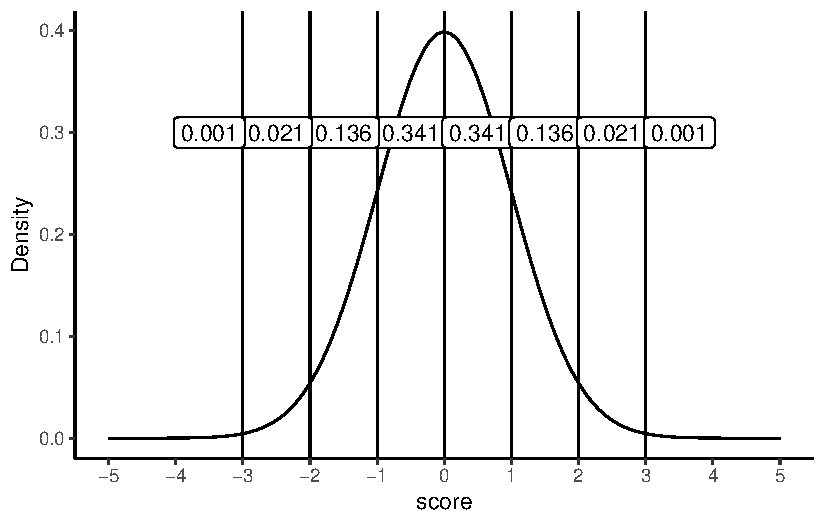
\includegraphics[width=0.75\textwidth,height=\textheight]{04-SamplesPopulations_files/figure-pdf/fig-4normalSDspercents-1.pdf}

}

\caption{\label{fig-4normalSDspercents}A normal distribution. Each line
represents a standard deviation from the mean. The labels show the
proportions of scores that fall between each bar.}

\end{figure}

The figure shows a normal distribution with mean = 0, and standard
deviation = 1. We've drawn lines at each of the standard deviations: -3,
-2, -1, 0, 1, 2, and 3. We also show some numbers in the labels, in
between each line. These numbers are proportions. For example, we see
the proportion is .341 for scores that fall between the range 0 and 1.
Scores between 0 and 1 occur 34.1\% of the time. Scores in between -1
and 1, occur 68.2\% of the time, that's more than half of the scores.
Scores between 1 and occur about 13.6\% of the time, and scores between
2 and 3 occur even less, only 2.1\% of the time.

Normal distributions always have these properties, even when they have
different means and standard deviations. For example, take a look at the
normal distribution in Figure~\ref{fig-4normalSDspercentsB} that has a
mean = 100, and standard deviation = 25.

\begin{figure}

{\centering 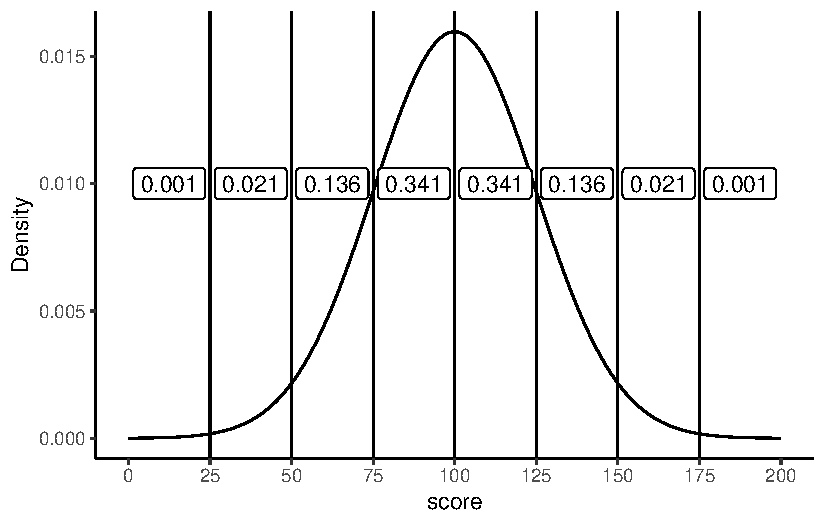
\includegraphics[width=0.75\textwidth,height=\textheight]{04-SamplesPopulations_files/figure-pdf/fig-4normalSDspercentsB-1.pdf}

}

\caption{\label{fig-4normalSDspercentsB}A normal distribution. Each line
represents a standard deviation from the mean. The labels show the
proportions of scores that fall between each bar.}

\end{figure}

Now we are looking at a normal distribution with mean = 100 and standard
deviation = 25. Notice that the region between 100 and 125 contains
34.1\% of the scores. This region is 1 standard deviation away from the
mean (the standard deviation is 25, the mean is 100, so 25 is one whole
standard deviation away from 100). As you can see, the very same
proportions occur between each of the standard deviations, as they did
when our standard deviation was set to 1 (with a mean of 0).

\hypertarget{idea-behind-z-scores}{%
\subsection{Idea behind z-scores}\label{idea-behind-z-scores}}

Sometimes it can be convenient to transform your original scores into
different scores that are easier to work with. For example, if you have
a bunch of proportions, like .3, .5, .6, .7, you might want to turn them
into percentages like 30\%, 50\%, 60\%, and 70\%. To do that you
multiply the proportions by a constant of 100. If you want to turn
percentages back into proportions, you divide by a constant of 100. This
kind of transformation just changes the scale of the numbers from
between 0-1, and between 0-100. Otherwise, the pattern in the numbers
stays the same.

The idea behind z-scores is a similar kind of transformation. The idea
is to express each raw score in terms of it's standard deviation. For
example, if I told you I got a 75\% on test, you wouldn't know how well
I did compared to the rest of the class. But, if I told you that I
scored 2 standard deviations above the mean, you'd know I did quite well
compared to the rest of the class, because you know that most scores (if
they are distributed normally) fall below 2 standard deviations of the
mean.

We also know, now thanks to the central limit theorem, that many of our
measures, such as sample means, will be distributed normally. So, it can
often be desirable to express the raw scores in terms of their standard
deviations.

Let's see how this looks in a table without showing you any formulas. We
will look at some scores that come from a normal distribution with mean
= 100, and standard deviation = 25. We will list some raw scores, along
with the z-scores

\begin{longtable}[]{@{}rr@{}}
\toprule\noalign{}
raw & z \\
\midrule\noalign{}
\endhead
\bottomrule\noalign{}
\endlastfoot
25 & -3 \\
50 & -2 \\
75 & -1 \\
100 & 0 \\
125 & 1 \\
150 & 2 \\
175 & 3 \\
\end{longtable}

Remember, the mean is 100, and the standard deviation is 25. How many
standard deviations away from the mean is a score of 100? The answer is
0, it's right on the mean. You can see the z-score for 100, is 0. How
many standard deviations is 125 away from the mean? Well the standard
deviation is 25, 125 is one whole 25 away from 100, that's a total of 1
standard deviation, so the z-score for 125 is 1. The z-score for 150 is
2, because 150 is two 25s away from 100. The z-score for 50 is -2,
because 50 is two 25s away from 100 in the opposite direction. All we
are doing here is re-expressing the raw scores in terms of how many
standard deviations they are from the mean. Remember, the mean is always
right on target, so the center of the z-score distribution is always 0.

\hypertarget{calculating-z-scores}{%
\subsection{Calculating z-scores}\label{calculating-z-scores}}

To calculate z-scores all you have to do is figure out how many standard
deviations from the mean each number is. Let's say the mean is 100, and
the standard deviation is 25. You have a score of 97. How many standard
deviations from the mean is 97?

First compute the difference between the score and the mean:

\(97-100 = -3\)

Alright, we have a total difference of -3. How many standard deviations
does -3 represent if 1 standard deviation is 25? Clearly -3 is much
smaller than 25, so it's going to be much less than 1. To figure it out,
just divide -3 by the standard deviation.

\(\frac{-3}{25} = -.12\)

Our z-score for 97 is -.12.

Here's the general formula:

\(z = \frac{\text{raw score} - \text{mean}}{\text{standard deviation}}\)

So, for example if we had these 10 scores from a normal distribution
with mean = 100, and standard deviation =25

\begin{verbatim}
#>  [1]  92.23  88.11 124.06  89.73 130.02 101.37  86.87 116.92 143.70  70.65
\end{verbatim}

The z-scores would be:

\begin{verbatim}
#>  [1] -0.3108 -0.4756  0.9624 -0.4108  1.2008  0.0548 -0.5252  0.6768  1.7480
#> [10] -1.1740
\end{verbatim}

Once you have the z-scores, you could use them as another way to
describe your data. For example, now just by looking at a score you know
if it is likely or unlikely to occur, because you know how the area
under the normal curve works. z-scores between -1 and 1 happen pretty
often, scores greater than 1 or -1 still happen fairly often, but not as
often. And, scores bigger than 2 or -2 don't happen very often. This is
a convenient thing to do if you want to look at your numbers and get a
general sense of how often they happen.

Usually you do not know the mean or the standard deviation of the
population that you are drawing your sample scores from. So, you could
use the mean and standard deviation of your sample as an estimate, and
then use those to calculate z-scores.

Finally, z-scores are also called \textbf{standardized scores}, because
each raw score is described in terms of it's standard deviation. This
may well be the last time we talk about z-scores in this book. You might
wonder why we even bothered telling you about them. First, it's worth
knowing they are a thing. Second, they become important as your
statistical prowess becomes more advanced. Third, some statistical
concepts, like correlation, can be re-written in terms of z-scores, and
this illuminates aspects of those statistics. Finally, they are super
useful when you are dealing with a normal distribution that has a known
mean and standard deviation.

\hypertarget{estimating-population-parameters}{%
\section{Estimating population
parameters}\label{estimating-population-parameters}}

Let's pause for a moment to get our bearings. We're about to go into the
topic of \textbf{estimation}. What is that, and why should you care?
First, population parameters are things about a distribution. For
example, distributions have means. The mean is a parameter of the
distribution. The standard deviation of a distribution is a parameter.
Anything that can describe a distribution is a potential parameter.

OK fine, who cares? This I think, is a really good question. There are
some good concrete reasons to care. And there are some great abstract
reasons to care. Unfortunately, most of the time in research, it's the
abstract reasons that matter most, and these can be the most difficult
to get your head around.

\hypertarget{concrete-population-parameters}{%
\subsection{Concrete population
parameters}\label{concrete-population-parameters}}

First some concrete reasons. There are real populations out there, and
sometimes you want to know the parameters of them. For example, if you
are a shoe company, you would want to know about the population
parameters of feet size. As a first pass, you would want to know the
mean and standard deviation of the population. If your company knew
this, and other companies did not, your company would do better
(assuming all shoes are made equal). Why would your company do better,
and how could it use the parameters? Here's one good reason. As a shoe
company you want to meet demand with the right amount of supply. If you
make too many big or small shoes, and there aren't enough people to buy
them, then you're making extra shoes that don't sell. If you don't make
enough of the most popular sizes, you'll be leaving money on the table.
Right? Yes. So, what would be an optimal thing to do? Perhaps, you would
make different amounts of shoes in each size, corresponding to how the
demand for each shoe size. You would know something about the demand by
figuring out the frequency of each size in the population. You would
need to know the population parameters to do this.

Fortunately, it's pretty easy to get the population parameters without
measuring the entire population. Who has time to measure every-bodies
feet? Nobody, that's who. Instead, you would just need to randomly pick
a bunch of people, measure their feet, and then measure the parameters
of the sample. If you take a big enough sample, we have learned that the
sample mean gives a very good estimate of the population mean. We will
learn shortly that a version of the standard deviation of the sample
also gives a good estimate of the standard deviation of the population.
Perhaps shoe-sizes have a slightly different shape than a normal
distribution. Here too, if you collect a big enough sample, the shape of
the distribution of the sample will be a good estimate of the shape of
the populations. All of these are good reasons to care about estimating
population parameters. But, do you run a shoe company? Probably not.

\hypertarget{abstract-population-parameters}{%
\subsection{Abstract population
parameters}\label{abstract-population-parameters}}

Even when we think we are talking about something concrete in
Psychology, it often gets abstract right away. Instead of measuring the
population of feet-sizes, how about the population of human happiness.
We all think we know what happiness is, everyone has more or less of it,
there are a bunch of people, so there must be a population of happiness
right? Perhaps, but it's not very concrete. The first problem is
figuring out how to measure happiness. Let's use a questionnaire.
Consider these questions:

\begin{quote}
How happy are you right now on a scale from 1 to 7? How happy are you in
general on a scale from 1 to 7? How happy are you in the mornings on a
scale from 1 to 7? How happy are you in the afternoons on a scale from 1
to 7?
\end{quote}

\begin{enumerate}
\def\labelenumi{\arabic{enumi}.}
\tightlist
\item
  = very unhappy
\item
  = unhappy
\item
  = sort of unhappy
\item
  = in the middle
\item
  = sort of happy
\item
  = happy
\item
  = very happy
\end{enumerate}

Forget about asking these questions to everybody in the world. Let's
just ask them to lots of people (our sample). What do you think would
happen? Well, obviously people would give all sorts of answers right. We
could tally up the answers and plot them in a histogram. This would show
us a distribution of happiness scores from our sample. ``Great,
fantastic!'', you say. Yes, fine and dandy.

So, on the one hand we could say lots of things about the people in our
sample. We could say exactly who says they are happy and who says they
aren't, after all they just told us!

But, what can we say about the larger population? Can we use the
parameters of our sample (e.g., mean, standard deviation, shape etc.) to
estimate something about a larger population. Can we infer how happy
everybody else is, just from our sample? HOLD THE PHONE.

\hypertarget{complications-with-inference}{%
\subsubsection{Complications with
inference}\label{complications-with-inference}}

Before listing a bunch of complications, let me tell you what I think we
can do with our sample. Provided it is big enough, our sample parameters
will be a pretty good estimate of what another sample would look like.
Because of the following discussion, this is often all we can say. But,
that's OK, as you see throughout this book, we can work with that!

\textbf{Problem 1: Multiple populations}: If you looked at a large
sample of questionnaire data you will find evidence of multiple
distributions inside your sample. People answer questions differently.
Some people are very cautious and not very extreme. Their answers will
tend to be distributed about the middle of the scale, mostly 3s, 4s, and
5s. Some people are very bi-modal, they are very happy and very unhappy,
depending on time of day. These people's answers will be mostly 1s and
2s, and 6s and 7s, and those numbers look like they come from a
completely different distribution. Some people are entirely happy or
entirely unhappy. Again, these two ``populations'' of people's numbers
look like two different distributions, one with mostly 6s and 7s, and
one with mostly 1s and 2s. Other people will be more random, and their
scores will look like a uniform distribution. So, is there a single
population with parameters that we can estimate from our sample?
Probably not. Could be a mixture of lots of populations with different
distributions.

\textbf{Problem 2: What do these questions measure?}: If the whole point
of doing the questionnaire is to estimate the population's happiness, we
really need wonder if the sample measurements actually tell us anything
about happiness in the first place. Some questions: Are people accurate
in saying how happy they are? Does the measure of happiness depend on
the scale, for example, would the results be different if we used 0-100,
or -100 to +100, or no numbers? Does the measure of happiness depend on
the wording in the question? Does a measure like this one tell us
everything we want to know about happiness (probably not), what is it
missing (who knows? probably lots). In short, nobody knows if these
kinds of questions measure what we want them to measure. We just hope
that they do. Instead, we have a very good idea of the kinds of things
that they actually measure. It's really quite obvious, and staring you
in the face. Questionnaire measurements measure how people answer
questionnaires. In other words, how people behave and answer questions
when they are given a questionnaire. This might also measure something
about happiness, when the question has to do about happiness. But, it
turns out people are remarkably consistent in how they answer questions,
even when the questions are total nonsense, or have no questions at all
(just numbers to choose!) Maul (2017).

The take home complications here are that we can collect samples, but in
Psychology, we often don't have a good idea of the populations that
might be linked to these samples. There might be lots of populations, or
the populations could be different depending on who you ask. Finally,
the ``population'' might not be the one you want it to be.

\hypertarget{experiments-and-population-parameters}{%
\subsection{Experiments and Population
parameters}\label{experiments-and-population-parameters}}

OK, so we don't own a shoe company, and we can't really identify the
population of interest in Psychology, can't we just skip this section on
estimation? After all, the ``population'' is just too weird and abstract
and useless and contentious. HOLD THE PHONE AGAIN!

It turns out we can apply the things we have been learning to solve lots
of important problems in research. These allow us to answer questions
with the data that we collect. Parameter estimation is one of these
tools. We just need to be a little bit more creative, and a little bit
more abstract to use the tools.

Here is what we know already. The numbers that we measure come from
somewhere, we have called this place ``distributions''. Distributions
control how the numbers arrive. Some numbers happen more than others
depending on the distribution. We assume, even if we don't know what the
distribution is, or what it means, that the numbers came from one.
Second, when get some numbers, we call it a sample. This entire chapter
so far has taught you one thing. When your sample is big, it resembles
the distribution it came from. And, when your sample is big, it will
resemble very closely what another big sample of the same thing will
look like. We can use this knowledge!

Very often as Psychologists what we want to know is what causes what. We
want to know if X causes something to change in Y. Does eating chocolate
make you happier? Does studying improve your grades? There a bazillions
of these kinds of questions. And, we want answers to them.

I've been trying to be mostly concrete so far in this textbook, that's
why we talk about silly things like chocolate and happiness, at least
they are concrete. Let's give a go at being abstract. We can do it.

So, we want to know if X causes Y to change. What is X? What is Y? X is
something you change, something you manipulate, the independent
variable. Y is something you measure. So, we will be taking samples from
Y. ``Oh I get it, we'll take samples from Y, then we can use the sample
parameters to estimate the population parameters of Y!'' NO, not really,
but yes sort of. We will take sample from Y, that is something we
absolutely do. In fact, that is really all we ever do, which is why
talking about the population of Y is kind of meaningless. We're more
interested in our samples of Y, and how they behave.

So, what would happen if we removed X from the universe altogether, and
then took a big sample of Y. We'll pretend Y measures something in a
Psychology experiment. So, we know right away that Y is variable. When
we take a big sample, it will have a distribution (because Y is
variable). So, we can do things like measure the mean of Y, and measure
the standard deviation of Y, and anything else we want to know about Y.
Fine. What would happen if we replicated this measurement. That is, we
just take another random sample of Y, just as big as the first. What
should happen is that our first sample should look a lot like our second
example. After all, we didn't do anything to Y, we just took two big
samples twice. Both of our samples will be a little bit different (due
to sampling error), but they'll be mostly the same. The bigger our
samples, the more they will look the same, especially when we don't do
anything to cause them to be different. In other words, we can use the
parameters of one sample to estimate the parameters of a second sample,
because they will tend to be the same, especially when they are large.

We are now ready for step two. You want to know if X changes Y. What do
you do? You make X go up and take a big sample of Y then look at it. You
make X go down, then take a second big sample of Y and look at it. Next,
you compare the two samples of Y. If X does nothing then what should you
find? We already discussed that in the previous paragraph. If X does
nothing, then both of your big samples of Y should be pretty similar.
However, if X does something to Y, then one of your big samples of Y
will be different from the other. You will have changed something about
Y. Maybe X makes the mean of Y change. Or maybe X makes the variation in
Y change. Or, maybe X makes the whole shape of the distribution change.
If we find any big changes that can't be explained by sampling error,
then we can conclude that something about X caused a change in Y! We
could use this approach to learn about what causes what!

The very important idea is still about estimation, just not population
parameter estimation exactly. We know that when we take samples they
naturally vary. So, when we estimate a parameter of a sample, like the
mean, we know we are off by some amount. When we find that two samples
are different, we need to find out if the size of the difference is
consistent with what sampling error can produce, or if the difference is
bigger than that. If the difference is bigger, then we can be confident
that sampling error didn't produce the difference. So, we can
confidently infer that something else (like an X) did cause the
difference. This bit of abstract thinking is what most of the rest of
the textbook is about. Determining whether there is a difference caused
by your manipulation. There's more to the story, there always is. We can
get more specific than just, is there a difference, but for introductory
purposes, we will focus on the finding of differences as a foundational
concept.

\hypertarget{interim-summary}{%
\subsection{Interim summary}\label{interim-summary}}

We've talked about estimation without doing any estimation, so in the
next section we will do some estimating of the mean and of the standard
deviation. Formally, we talk about this as using a sample to estimate a
parameter of the population. Feel free to think of the ``population'' in
different ways. It could be concrete population, like the distribution
of feet-sizes. Or, it could be something more abstract, like the
parameter estimate of what samples usually look like when they come from
a distribution.

\hypertarget{estimating-the-population-mean}{%
\subsection{Estimating the population
mean}\label{estimating-the-population-mean}}

Suppose we go to Brooklyn and 100 of the locals are kind enough to sit
through an IQ test. The average IQ score among these people turns out to
be \(\bar{X}=98.5\). So what is the true mean IQ for the entire
population of Brooklyn? Obviously, we don't know the answer to that
question. It could be \(97.2\), but if could also be \(103.5\). Our
sampling isn't exhaustive so we cannot give a definitive answer.
Nevertheless if forced to give a ``best guess'' I'd have to say
\(98.5\). That's the essence of statistical estimation: giving a best
guess. We're using the sample mean as the best guess of the population
mean.

In this example, estimating the unknown population parameter is
straightforward. I calculate the sample mean, and I use that as my
\textbf{estimate of the population mean}. It's pretty simple, and in the
next section we'll explain the statistical justification for this
intuitive answer. However, for the moment let's make sure you recognize
that the sample statistic and the estimate of the population parameter
are conceptually different things. A sample statistic is a description
of your data, whereas the estimate is a guess about the population. With
that in mind, statisticians often use different notation to refer to
them. For instance, if true population mean is denoted \(\mu\), then we
would use \(\hat\mu\) to refer to our estimate of the population mean.
In contrast, the sample mean is denoted \(\bar{X}\) or sometimes \(m\).
However, in simple random samples, the estimate of the population mean
is identical to the sample mean: if I observe a sample mean of
\(\bar{X} = 98.5\), then my estimate of the population mean is also
\(\hat\mu = 98.5\). To help keep the notation clear, here's a handy
table:

\begin{longtable}[]{@{}
  >{\raggedright\arraybackslash}p{(\columnwidth - 4\tabcolsep) * \real{0.2603}}
  >{\raggedright\arraybackslash}p{(\columnwidth - 4\tabcolsep) * \real{0.3562}}
  >{\raggedright\arraybackslash}p{(\columnwidth - 4\tabcolsep) * \real{0.3836}}@{}}
\toprule\noalign{}
\begin{minipage}[b]{\linewidth}\raggedright
Symbol
\end{minipage} & \begin{minipage}[b]{\linewidth}\raggedright
What is it?
\end{minipage} & \begin{minipage}[b]{\linewidth}\raggedright
Do we know what it is?
\end{minipage} \\
\midrule\noalign{}
\endhead
\bottomrule\noalign{}
\endlastfoot
\(\bar{X}\) & Sample mean & Yes, calculated from the raw data \\
\(\mu\) & True population mean & Almost never known for sure \\
\(\hat{\mu}\) & Estimate of the population mean & Yes, identical to the
sample mean \\
\end{longtable}

\hypertarget{estimating-the-population-standard-deviation}{%
\subsection{Estimating the population standard
deviation}\label{estimating-the-population-standard-deviation}}

So far, estimation seems pretty simple, and you might be wondering why I
forced you to read through all that stuff about sampling theory. In the
case of the mean, our estimate of the population parameter
(i.e.~\(\hat\mu\)) turned out to identical to the corresponding sample
statistic (i.e.~\(\bar{X}\)). However, that's not always true. To see
this, let's have a think about how to construct an \textbf{estimate of
the population standard deviation}, which we'll denote \(\hat\sigma\).
What shall we use as our estimate in this case? Your first thought might
be that we could do the same thing we did when estimating the mean, and
just use the sample statistic as our estimate. That's almost the right
thing to do, but not quite.

Here's why. Suppose I have a sample that contains a single observation.
For this example, it helps to consider a sample where you have no
intuitions at all about what the true population values might be, so
let's use something completely fictitious. Suppose the observation in
question measures the \textbf{cromulence} of my shoes. It turns out that
my shoes have a cromulence of 20. So here's my sample:

\texttt{20}

This is a perfectly legitimate sample, even if it does have a sample
size of \(N=1\). It has a sample mean of 20, and because every
observation in this sample is equal to the sample mean (obviously!) it
has a sample standard deviation of 0. As a description of the
\textbf{sample} this seems quite right: the sample contains a single
observation and therefore there is no variation observed within the
sample. A sample standard deviation of \(s = 0\) is the right answer
here. But as an estimate of the \textbf{population} standard deviation,
it feels completely insane, right? Admittedly, you and I don't know
anything at all about what ``cromulence'' is, but we know something
about data: the only reason that we don't see any variability in the
\textbf{sample} is that the sample is too small to display any
variation! So, if you have a sample size of \(N=1\), it \textbf{feels}
like the right answer is just to say ``no idea at all''.

Notice that you \textbf{don't} have the same intuition when it comes to
the sample mean and the population mean. If forced to make a best guess
about the population mean, it doesn't feel completely insane to guess
that the population mean is 20. Sure, you probably wouldn't feel very
confident in that guess, because you have only the one observation to
work with, but it's still the best guess you can make.

Let's extend this example a little. Suppose I now make a second
observation. My data set now has \(N=2\) observations of the cromulence
of shoes, and the complete sample now looks like this:

\texttt{20,\ 22}

This time around, our sample is \textbf{just} large enough for us to be
able to observe some variability: two observations is the bare minimum
number needed for any variability to be observed! For our new data set,
the sample mean is \(\bar{X}=21\), and the sample standard deviation is
\(s=1\). What intuitions do we have about the population? Again, as far
as the population mean goes, the best guess we can possibly make is the
sample mean: if forced to guess, we'd probably guess that the population
mean cromulence is 21. What about the standard deviation? This is a
little more complicated. The sample standard deviation is only based on
two observations, and if you're at all like me you probably have the
intuition that, with only two observations, we haven't given the
population ``enough of a chance'' to reveal its true variability to us.
It's not just that we suspect that the estimate is \textbf{wrong}: after
all, with only two observations we expect it to be wrong to some degree.
The worry is that the error is \textbf{systematic}.

If the error is systematic, that means it is \textbf{biased}. For
example, imagine if the sample mean was always smaller than the
population mean. If this was true (it's not), then we couldn't use the
sample mean as an estimator. It would be biased, we'd be using the wrong
number.

It turns out the sample standard deviation is a \textbf{biased
estimator} of the population standard deviation. We can sort of
anticipate this by what we've been discussing. When the sample size is
1, the standard deviation is 0, which is obviously to small. When the
sample size is 2, the standard deviation becomes a number bigger than 0,
but because we only have two sample, we suspect it might still be too
small. Turns out this intuition is correct.

It would be nice to demonstrate this somehow. There are in fact
mathematical proofs that confirm this intuition, but unless you have the
right mathematical background they don't help very much. Instead, what
I'll do is use R to simulate the results of some experiments. With that
in mind, let's return to our IQ studies. Suppose the true population
mean IQ is 100 and the standard deviation is 15. I can use the
\textbf{rnorm()} function to generate the the results of an experiment
in which I measure \(N=2\) IQ scores, and calculate the sample standard
deviation. If I do this over and over again, and plot a histogram of
these sample standard deviations, what I have is the \textbf{sampling
distribution of the standard deviation}. I've plotted this distribution
in Figure~\ref{fig-sampdistsd}.

\begin{figure}

{\centering 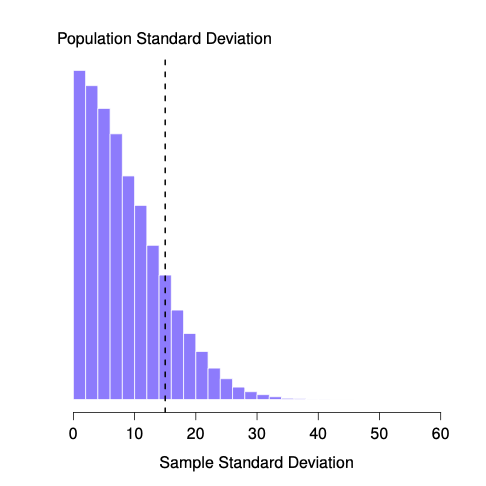
\includegraphics[width=0.75\textwidth,height=\textheight]{imgs/navarro_img/estimation/sampdistsd.png}

}

\caption{\label{fig-sampdistsd}The sampling distribution of the sample
standard deviation for a two IQ scores experiment. The true population
standard deviation is 15 (dashed line), but as you can see from the
histogram, the vast majority of experiments will produce a much smaller
sample standard deviation than this. On average, this experiment would
produce a sample standard deviation of only 8.5, well below the true
value! In other words, the sample standard deviation is a biased
estimate of the population standard deviation.}

\end{figure}

Even though the true population standard deviation is 15, the average of
the \textbf{sample} standard deviations is only 8.5. Notice that this is
a very different from when we were plotting sampling distributions of
the sample mean, those were always centered around the mean of the
population.

Now let's extend the simulation. Instead of restricting ourselves to the
situation where we have a sample size of \(N=2\), let's repeat the
exercise for sample sizes from 1 to 10. If we plot the average sample
mean and average sample standard deviation as a function of sample size,
you get the following results.

@fig-estimatorbiasA shows the sample mean as a function of sample size.
Notice it's a flat line. The sample mean doesn't underestimate or
overestimate the population mean. It is an unbiased estimate!

\begin{figure}

{\centering 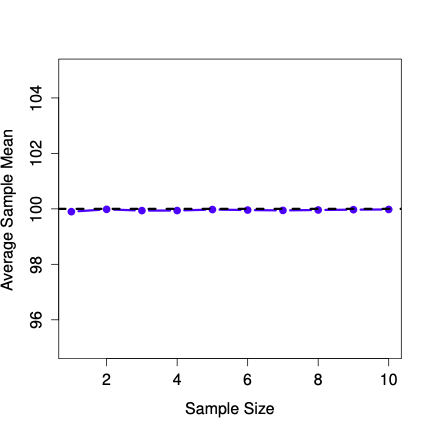
\includegraphics[width=0.75\textwidth,height=\textheight]{imgs/navarro_img/estimation/biasMean-eps-converted-to.png}

}

\caption{\label{fig-estimatorbiasA}An illustration of the fact that the
sample mean is an unbiased estimator of the population mean.}

\end{figure}

Figure~\ref{fig-estimatorbiasB} shows the sample standard deviation as a
function of sample size. Notice it is not a flat line. The sample
standard deviation systematically underestimates the population standard
deviation!

\begin{figure}

{\centering 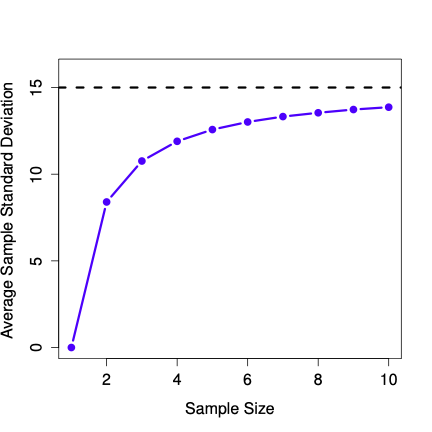
\includegraphics[width=0.75\textwidth,height=\textheight]{imgs/navarro_img/estimation/biasSD-eps-converted-to.png}

}

\caption{\label{fig-estimatorbiasB}An illustration of the fact that the
the sample standard deviation is a biased estimator of the population
standard deviation.}

\end{figure}

In other words, if we want to make a ``best guess'' (\(\hat\sigma\), our
estimate of the population standard deviation) about the value of the
population standard deviation \(\sigma\), we should make sure our guess
is a little bit larger than the sample standard deviation \(s\).

The fix to this systematic bias turns out to be very simple. Here's how
it works. Before tackling the standard deviation, let's look at the
variance. If you recall from the second chapter, the sample variance is
defined to be the average of the squared deviations from the sample
mean. That is: \[s^2 = \frac{1}{N} \sum_{i=1}^N (X_i - \bar{X})^2\] The
sample variance \(s^2\) is a biased estimator of the population variance
\(\sigma^2\). But as it turns out, we only need to make a tiny tweak to
transform this into an unbiased estimator. All we have to do is divide
by \(N-1\) rather than by \(N\). If we do that, we obtain the following
formula: \[\hat\sigma^2 = \frac{1}{N-1} \sum_{i=1}^N (X_i - \bar{X})^2\]
This is an unbiased estimator of the population variance \(\sigma\).

A similar story applies for the standard deviation. If we divide by
\(N-1\) rather than \(N\), our estimate of the population standard
deviation becomes:
\[\hat\sigma = \sqrt{\frac{1}{N-1} \sum_{i=1}^N (X_i - \bar{X})^2}\].

It is worth pointing out that software programs make assumptions
\textbf{for you}, about which variance and standard deviation
\textbf{you} are computing. Some programs automatically divide by
\(N-1\), some do not. You need to check to figure out what they are
doing. Don't let the software tell you what to do. Software is for you
telling it what to do.

One final point: in practice, a lot of people tend to refer to
\(\hat{\sigma}\) (i.e., the formula where we divide by \(N-1\)) as the
\textbf{sample} standard deviation. Technically, this is incorrect: the
\textbf{sample} standard deviation should be equal to \(s\) (i.e., the
formula where we divide by \(N\)). These aren't the same thing, either
conceptually or numerically. One is a property of the sample, the other
is an estimated characteristic of the population. However, in almost
every real life application, what we actually care about is the estimate
of the population parameter, and so people always report \(\hat\sigma\)
rather than \(s\).

\begin{tcolorbox}[enhanced jigsaw, breakable, colback=white, coltitle=black, toptitle=1mm, rightrule=.15mm, title=\textcolor{quarto-callout-note-color}{\faInfo}\hspace{0.5em}{Note}, opacitybacktitle=0.6, opacityback=0, colframe=quarto-callout-note-color-frame, leftrule=.75mm, colbacktitle=quarto-callout-note-color!10!white, arc=.35mm, bottomtitle=1mm, titlerule=0mm, bottomrule=.15mm, toprule=.15mm, left=2mm]

Note, whether you should divide by N or N-1 also depends on your
philosophy about what you are doing. For example, if you don't think
that what you are doing is estimating a population parameter, then why
would you divide by N-1? Also, when N is large, it doesn't matter too
much. The difference between a big N, and a big N-1, is just -1.

\end{tcolorbox}

This is the right number to report, of course, it's that people tend to
get a little bit imprecise about terminology when they write it up,
because ``sample standard deviation'' is shorter than ``estimated
population standard deviation''. It's no big deal, and in practice I do
the same thing everyone else does. Nevertheless, I think it's important
to keep the two \textbf{concepts} separate: it's never a good idea to
confuse ``known properties of your sample'' with ``guesses about the
population from which it came''. The moment you start thinking that
\(s\) and \(\hat\sigma\) are the same thing, you start doing exactly
that.

To finish this section off, here's another couple of tables to help keep
things clear:

\begin{longtable}[]{@{}
  >{\raggedright\arraybackslash}p{(\columnwidth - 4\tabcolsep) * \real{0.2639}}
  >{\raggedright\arraybackslash}p{(\columnwidth - 4\tabcolsep) * \real{0.3333}}
  >{\raggedright\arraybackslash}p{(\columnwidth - 4\tabcolsep) * \real{0.4028}}@{}}
\toprule\noalign{}
\begin{minipage}[b]{\linewidth}\raggedright
Symbol
\end{minipage} & \begin{minipage}[b]{\linewidth}\raggedright
What is it?
\end{minipage} & \begin{minipage}[b]{\linewidth}\raggedright
Do we know what it is?
\end{minipage} \\
\midrule\noalign{}
\endhead
\bottomrule\noalign{}
\endlastfoot
\(s^2\) & Sample variance & Yes, calculated from the raw data \\
\(\sigma^2\) & Population variance & Almost never known for sure \\
\(\hat{\sigma}^2\) & Estimate of the population variance & Yes, but not
the same as the sample variance \\
\end{longtable}

\hypertarget{estimating-a-confidence-interval}{%
\section{Estimating a confidence
interval}\label{estimating-a-confidence-interval}}

\begin{quote}
Statistics means never having to say you're certain -- Unknown origin
\end{quote}

Up to this point in this chapter, we've outlined the basics of sampling
theory which statisticians rely on to make guesses about population
parameters on the basis of a sample of data. As this discussion
illustrates, one of the reasons we need all this sampling theory is that
every data set leaves us with some of uncertainty, so our estimates are
never going to be perfectly accurate. The thing that has been missing
from this discussion is an attempt to \textbf{quantify} the amount of
uncertainty in our estimate. It's not enough to be able guess that the
mean IQ of undergraduate psychology students is 115 (yes, I just made
that number up). We also want to be able to say something that expresses
the degree of certainty that we have in our guess. For example, it would
be nice to be able to say that there is a 95\% chance that the true mean
lies between 109 and 121. The name for this is a \textbf{confidence
interval} for the mean.

Armed with an understanding of sampling distributions, constructing a
confidence interval for the mean is actually pretty easy. Here's how it
works. Suppose the true population mean is \(\mu\) and the standard
deviation is \(\sigma\). I've just finished running my study that has
\(N\) participants, and the mean IQ among those participants is
\(\bar{X}\). We know from our discussion of the central limit theorem
that the sampling distribution of the mean is approximately normal. We
also know from our discussion of the normal distribution that there is a
95\% chance that a normally-distributed quantity will fall within two
standard deviations of the true mean. To be more precise, we can use the
\textbf{qnorm()} function to compute the 2.5th and 97.5th percentiles of
the normal distribution

\begin{quote}
qnorm( p = c(.025, .975) ) {[}1{]} -1.959964 1.959964
\end{quote}

Okay, so I lied earlier on. The more correct answer is that a 95\%
chance that a normally-distributed quantity will fall within 1.96
standard deviations of the true mean.

Next, recall that the standard deviation of the sampling distribution is
referred to as the standard error, and the standard error of the mean is
written as SEM. When we put all these pieces together, we learn that
there is a 95\% probability that the sample mean \(\bar{X}\) that we
have actually observed lies within 1.96 standard errors of the
population mean. Oof, that is a lot of mathy talk there. We'll clear it
up, don't worry.

Mathematically, we write this as:
\[\mu - \left( 1.96 \times \mbox{SEM} \right) \ \leq \  \bar{X}\  \leq \  \mu + \left( 1.96 \times \mbox{SEM} \right)\]
where the SEM is equal to \(\sigma / \sqrt{N}\), and we can be 95\%
confident that this is true.

However, that's not answering the question that we're actually
interested in. The equation above tells us what we should expect about
the sample mean, given that we know what the population parameters are.
What we \textbf{want} is to have this work the other way around: we want
to know what we should believe about the population parameters, given
that we have observed a particular sample. However, it's not too
difficult to do this. Using a little high school algebra, a sneaky way
to rewrite our equation is like this:
\[\bar{X} -  \left( 1.96 \times \mbox{SEM} \right) \ \leq \ \mu  \ \leq  \ \bar{X} +  \left( 1.96 \times \mbox{SEM}\right)\]
What this is telling is is that the range of values has a 95\%
probability of containing the population mean \(\mu\). We refer to this
range as a \textbf{95\% confidence interval}, denoted
\(\mbox{CI}_{95}\). In short, as long as \(N\) is sufficiently large --
large enough for us to believe that the sampling distribution of the
mean is normal -- then we can write this as our formula for the 95\%
confidence interval:
\[\mbox{CI}_{95} = \bar{X} \pm \left( 1.96 \times \frac{\sigma}{\sqrt{N}} \right)\]
Of course, there's nothing special about the number 1.96: it just
happens to be the multiplier you need to use if you want a 95\%
confidence interval. If I'd wanted a 70\% confidence interval, I could
have used the \textbf{qnorm()} function to calculate the 15th and 85th
quantiles:

\begin{quote}
qnorm( p = c(.15, .85) ) {[}1{]} -1.036433 1.036433
\end{quote}

and so the formula for \(\mbox{CI}_{70}\) would be the same as the
formula for \(\mbox{CI}_{95}\) except that we'd use 1.04 as our magic
number rather than 1.96.

\hypertarget{a-slight-mistake-in-the-formula}{%
\subsection{A slight mistake in the
formula}\label{a-slight-mistake-in-the-formula}}

As usual, I lied. The formula that I've given above for the 95\%
confidence interval is approximately correct, but I glossed over an
important detail in the discussion. Notice my formula requires you to
use the standard error of the mean, SEM, which in turn requires you to
use the true population standard deviation \(\sigma\).

Yet, before we stressed the fact that we don't actually \textbf{know}
the true population parameters. Because we don't know the true value of
\(\sigma\), we have to use an estimate of the population standard
deviation \(\hat{\sigma}\) instead. This is pretty straightforward to
do, but this has the consequence that we need to use the quantiles of
the \(t\)-distribution rather than the normal distribution to calculate
our magic number; and the answer depends on the sample size. Plus, we
haven't really talked about the \(t\) distribution yet.

When we use the \(t\) distribution instead of the normal distribution,
we get bigger numbers, indicating that we have more uncertainty. And why
do we have that extra uncertainty? Well, because our estimate of the
population standard deviation \(\hat\sigma\) might be wrong! If it's
wrong, it implies that we're a bit less sure about what our sampling
distribution of the mean actually looks like\ldots{} and this
uncertainty ends up getting reflected in a wider confidence interval.

\hypertarget{summary-2}{%
\section{Summary}\label{summary-2}}

In this chapter I've covered two main topics. The first half of the
chapter talks about sampling theory, and the second half talks about how
we can use sampling theory to construct estimates of the population
parameters. The section breakdown looks like this:

\begin{itemize}
\item
  Basic ideas about samples, sampling and populations
\item
  Statistical theory of sampling: the law of large numbers, sampling
  distributions and the central limit theorem.
\item
  Estimating means and standard deviations
\item
  confidence intervals
\end{itemize}

As always, there's a lot of topics related to sampling and estimation
that aren't covered in this chapter, but for an introductory psychology
class this is fairly comprehensive I think. For most applied researchers
you won't need much more theory than this. One big question that I
haven't touched on in this chapter is what you do when you don't have a
simple random sample. There is a lot of statistical theory you can draw
on to handle this situation, but it's well beyond the scope of this
book.

\hypertarget{videos-2}{%
\section{Videos}\label{videos-2}}

\hypertarget{introduction-to-probability}{%
\subsection{Introduction to
Probability}\label{introduction-to-probability}}

Jeff has several more videos on probability that you can view on his
\href{https://www.youtube.com/playlist?list=PLKXdxQAT3tCvuex_E1ZnQYaw897ELUSaI}{statistics
playlist}.

\hypertarget{chebychevs-theorem}{%
\subsection{Chebychev's Theorem}\label{chebychevs-theorem}}

\hypertarget{z-scores-1}{%
\subsection{Z-scores}\label{z-scores-1}}

\hypertarget{normal-distribution-i}{%
\subsection{Normal Distribution I}\label{normal-distribution-i}}

\hypertarget{normal-distribution-ii}{%
\subsection{Normal Distribution II}\label{normal-distribution-ii}}

\bookmarksetup{startatroot}

\hypertarget{foundations-for-inference}{%
\chapter{Foundations for inference}\label{foundations-for-inference}}

\begin{quote}
Data and data sets are not objective; they are creations of human
design. We give numbers their voice, draw inferences from them, and
define their meaning through our interpretations. ---Katie Crawford
\end{quote}

So far we have been talking about describing data and looking for
possible relationships between things we measure. We began with the
problem of having too many numbers and discussed how they could be
summarized with descriptive statistics, and communicated in graphs. We
also looked at the idea of relationships between things. If one thing
causes change in another thing, then if we measure how one thing goes up
and down we should find that other thing goes up and down, or does
something systematically following the first thing. At the end of the
chapter on correlation, we showed how correlations, which imply a
relationship between two things, are very difficult to interpret. Why?
Because an observed correlation can be caused by a hidden third
variable, or could be a spurious finding ``caused'' by random chance. In
the last chapter, we talked about sampling from distributions, and we
saw how samples can be different because of random error introduced by
the sampling process.

Now we begin our journey into \textbf{inferential statistics}. These are
tools used to make inferences about where our data came from, and to
make inferences about what causes what.

In this chapter we provide some foundational ideas. We will stay mostly
at a conceptual level, and use lots of simulations like we did in the
last chapters. In the remaining chapters we formalize the intuitions
built here to explain how some common inferential statistics work.

\hypertarget{brief-review-of-experiments}{%
\section{Brief review of
Experiments}\label{brief-review-of-experiments}}

In chapter one we talked a about research methods and experiments.
Experiments are a structured way of collecting data that can permit
inferences about causality. If we wanted to know whether something like
watching cats on YouTube increases happiness we would need an
experiment. We already found out that just finding a bunch of people and
measuring number of hours watching cats, and level of happiness, and
correlating the two will not permit inferences about causation. For one,
the causal flow could be reversed. Maybe being happy causes people to
watch more cat videos. We need an experiment.

An experiment has two parts. A manipulation and a measurement. The
manipulation is under the control of the experimenter. Manipulations are
also called \textbf{independent variables}. For example, we could
manipulate time spent watching cat videos: 1 hour versus 2 hours of cat
videos. The measurement is the data that is collected. We could measure
how happy people are after watching cat videos on a scale from 1 to 100.
Measurements are also called \textbf{dependent variables}. So, in a
basic experiment like the one above, we take measurements of happiness
from people in one of two experimental conditions defined by the
independent variable. Let's say we ran 50 subjects. 25 subjects would be
randomly assigned to watch 1 hour of cat videos, and the other 25
subjects would be randomly assigned to watch 2 hours of cat videos. We
would measure happiness for each subject at the end of the videos. Then
we could look at the data.

What would we want to look at? If watching cat videos caused a change in
happiness, then we would expect the measures of happiness for people
watching 1 hour of cat videos to be different from the measures of
happiness for people watching 2 hours of cat videos. If watching cat
videos does not change happiness, then we would expect no differences in
measures of happiness between conditions. Causal forces cause change,
and the experiment is set up to detect the change.

Now we can state one overarching question, how do we know if the data
changed between conditions? If we can be confident that there was a
change between conditions, we can infer that our manipulation caused a
changed in the measurement. If we cannot be confident there was a
change, then we cannot infer that our manipulation caused a change in
the measurement. We need to build some change detection tools so we can
know a change when we find one.

``Hold on, if we are just looking for a change, wouldn't that be easy to
see by looking at the numbers and seeing if they are different, what's
so hard about that?''. Good question. Now we must take a detour. The
short answer is that there will always be change in the data (remember
variance).

\hypertarget{the-data-came-from-a-distribution}{%
\section{The data came from a
distribution}\label{the-data-came-from-a-distribution}}

In the last chapter we discussed samples and distributions, and the idea
that you can take samples from distributions. So, from now on when you
see a bunch of numbers, you should wonder, ``where did these numbers
come from?''. What caused some kinds of numbers to happen more than
other kinds of numbers. The answer to this question requires us to again
veer off into the abstract world of distributions. A
\textbf{distribution} a place where numbers can come from. The
distribution sets the constraints. It determines what numbers are likely
to occur, and what numbers are not likely to occur. Distributions are
abstract ideas. But, they can be made concrete, and we can draw them
with pictures that you have seen already, called histograms.

The next bit might seem slightly repetitive from the previous chapter.
We again look at sampling numbers from a uniform distribution. We show
that individual samples can look quite different from each other. Much
of the beginning part of this chapter will already be familiar to you,
but we take the concepts in a slightly different direction. The
direction is how to make inferences about the role of chance in your
experiment.

\hypertarget{uniform-distribution}{%
\subsection{Uniform distribution}\label{uniform-distribution}}

As a reminder from last chapter, Figure~\ref{fig-5unifagain} shows that
the shape of a uniform distribution is completely flat.

\begin{figure}

{\centering 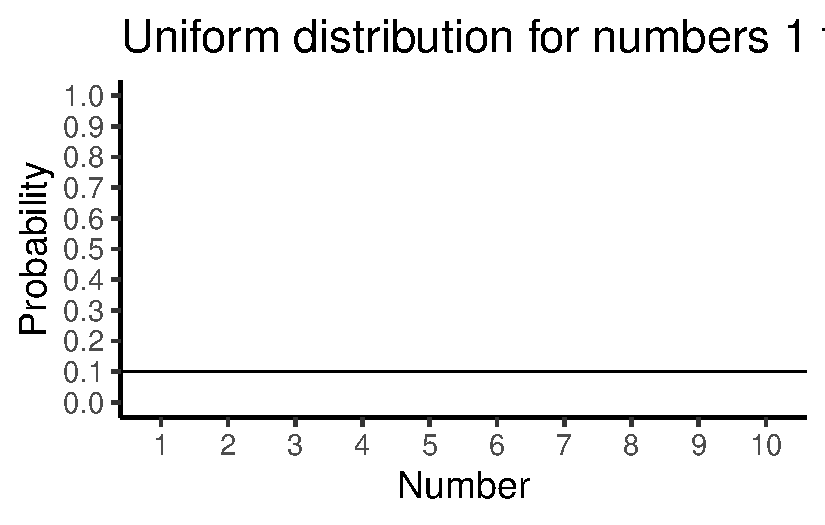
\includegraphics[width=0.75\textwidth,height=\textheight]{05-Foundation_Inference_files/figure-pdf/fig-5unifagain-1.pdf}

}

\caption{\label{fig-5unifagain}Uniform distribution showing that the
numbers from 1 to 10 have an equal probability of being sampled}

\end{figure}

OK, so that doesn't look like much. What is going on here? The y-axis is
labelled \texttt{probability}, and it goes from 0 to 1. The x-axis is
labelled \texttt{Number}, and it goes from one to 10. There is a
horizontal line drawn straight through. This line tells you the
probability of each number from 1 to 10. Notice the line is flat. This
means all of the numbers have the same probability of occurring. More
specifically, there are 10 numbers from 1 to 10 (1,2,3,4,5,6,7,8,9,10),
and they all have an equal chance of occurring. 1/10 = .1, which is the
probability indicated by the horizontal line.

``So what?''. Imagine that this uniform distribution is a number
generating machine. It spits out numbers, but it spits out each number
with the probability indicated by the line. If this distribution was
going to start spitting out numbers, it would spit out 10\% 1s, 10\% 2s,
10\% 3s, and so on, up to 10\% 10s. Wanna see what that would look like?
Let's make it spit out 100 numbers and put them in
Table~\ref{tbl-5100rand}.

\hypertarget{tbl-5100rand}{}
\begin{longtable}[]{@{}rrrrrrrrrr@{}}
\caption{\label{tbl-5100rand}100 numbers randomly sampled from a uniform
distribution.}\tabularnewline
\toprule\noalign{}
\endfirsthead
\endhead
\bottomrule\noalign{}
\endlastfoot
2 & 4 & 4 & 3 & 7 & 3 & 7 & 10 & 3 & 6 \\
9 & 8 & 5 & 3 & 4 & 5 & 4 & 3 & 8 & 9 \\
6 & 3 & 5 & 5 & 6 & 7 & 7 & 9 & 2 & 6 \\
7 & 5 & 6 & 1 & 2 & 6 & 6 & 9 & 1 & 5 \\
9 & 1 & 5 & 5 & 8 & 10 & 7 & 8 & 7 & 7 \\
4 & 6 & 9 & 8 & 2 & 8 & 2 & 1 & 3 & 8 \\
4 & 7 & 8 & 5 & 3 & 3 & 2 & 6 & 2 & 2 \\
4 & 5 & 10 & 1 & 9 & 6 & 8 & 2 & 4 & 7 \\
1 & 6 & 8 & 6 & 10 & 6 & 2 & 6 & 7 & 8 \\
1 & 5 & 6 & 6 & 5 & 4 & 9 & 1 & 1 & 1 \\
\end{longtable}

We used the uniform distribution to generate these numbers. Officially,
we call this \textbf{sampling} from a \textbf{distribution}. Sampling is
what you do at a grocery store when there is free food. You can keep
taking more. However, if you take all of the samples, then what you have
is called the \textbf{population}. We'll talk more about samples and
populations as we go along.

Because we used the uniform distribution to create numbers, we already
know where our numbers came from. However, we can still pretend for the
moment that someone showed up at your door, showed you these numbers,
and then you wondered where they came from. Can you tell just by looking
at these numbers that they came from a uniform distribution? What would
need to look at? Perhaps you would want to know if all of the numbers
occur with roughly equal frequency, after all they should have right?
That is, if each number had the same chance of occurring, we should see
that each number occurs roughly the same number of times.

We already know what a histogram is, so we can put our sample of 100
numbers into a histogram and see what the counts look like. If all of
the numbers from 1 to 10 occur with equal frequency, then each
individual number should occur about 10 times.
Figure~\ref{fig-5histunif} shows the histogram:

\begin{figure}

{\centering 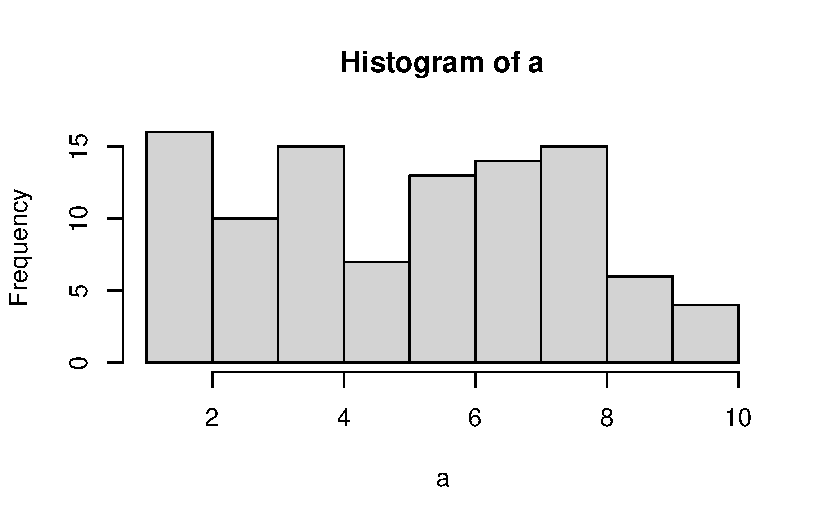
\includegraphics[width=0.75\textwidth,height=\textheight]{05-Foundation_Inference_files/figure-pdf/fig-5histunif-1.pdf}

}

\caption{\label{fig-5histunif}Histogram of 100 numbers randomly sampled
from the uniform distribution containing the integers from 1 to 10}

\end{figure}

Uh oh, as you can see, not all of the number occurred 10 times each. All
of the bars are not the same height. This shows that randomly sampling
numbers from this distribution does not guarantee that our numbers will
be exactly like the distribution they came from. We can call this
sampling error, or sampling variability.

\hypertarget{not-all-samples-are-the-same-they-are-usually-quite-different}{%
\subsection{Not all samples are the same, they are usually quite
different}\label{not-all-samples-are-the-same-they-are-usually-quite-different}}

Let's look at sampling error more closely. We will sample 20 numbers
from the uniform distribution. We should expect that each number between
1 and 10 occurs about two times each. As before, this expectation can be
visualized in a histogram. To get a better sense of sampling error,
let's repeat the above process ten times. Figure~\ref{fig-5manysamples}
has 10 histograms, each showing what 10 different samples of twenty
numbers looks like:

\begin{figure}

{\centering 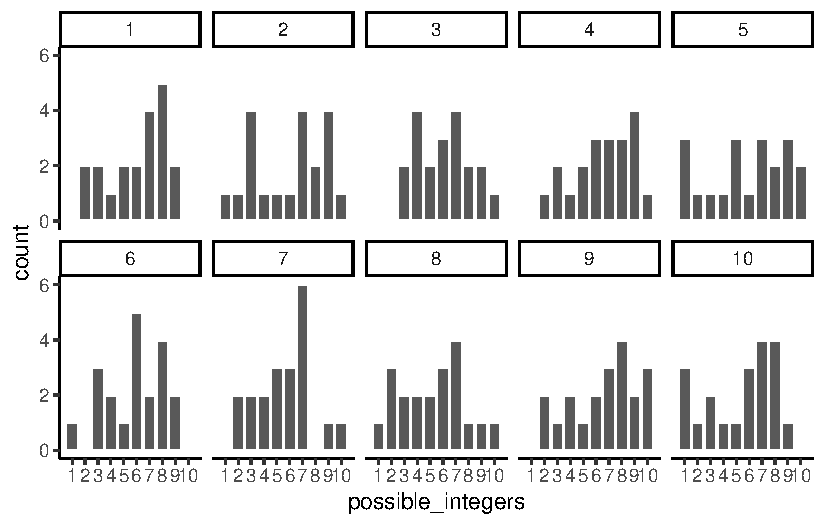
\includegraphics[width=1\textwidth,height=\textheight]{05-Foundation_Inference_files/figure-pdf/fig-5manysamples-1.pdf}

}

\caption{\label{fig-5manysamples}Histograms for 10 different samples
from the uniform distribution. Each sample contains 20 numbers. The
histograms all look quite different. The differences between the samples
are due to sampling error or random chance.}

\end{figure}

You might notice right away that none of the histograms are the same.
Even though we are randomly taking 20 numbers from the very same uniform
distribution, each sample of 20 numbers comes out different. This is
sampling variability, or sampling error.

\textbf{?@fig-5expectedUnif} shows an animated version of the process of
repeatedly choosing 20 new random numbers and plotting a histogram. The
horizontal line shows the flat-line shape of the uniform distribution.
The line crosses the y-axis at 2; and, we expect that each number (from
1 to 10) should occur about 2 times each in a sample of 20. However,
each sample bounces around quite a bit, due to random chance.

Looking at the above histograms shows us that figuring out where our
numbers came from can be difficult. In the real world, our measurements
are samples. We usually only have the luxury of getting one sample of
measurements, rather than repeating our own measurements 10 times or
more. If you look at the histograms, you will see that some of them look
like they could have come from the uniform distribution: most of the
bars are near two, and they all fall kind of on a flat line. But, if you
happen to look at a different sample, you might see something that is
very bumpy, with some numbers happening way more than others. This could
suggest to you that those numbers did not come from a uniform
distribution (they're just too bumpy). But let me remind you, all of
these samples came from a uniform distribution, this is what samples
from that distribution look like. This is what chance does to samples,
it makes the individual data points noisy.

\hypertarget{large-samples-are-more-like-the-distribution-they-came-from}{%
\subsection{Large samples are more like the distribution they came
from}\label{large-samples-are-more-like-the-distribution-they-came-from}}

Let's refresh the question. Which of the two samples in
Figure~\ref{fig-5whichone} do you think came from a uniform
distribution?

\begin{figure}

{\centering 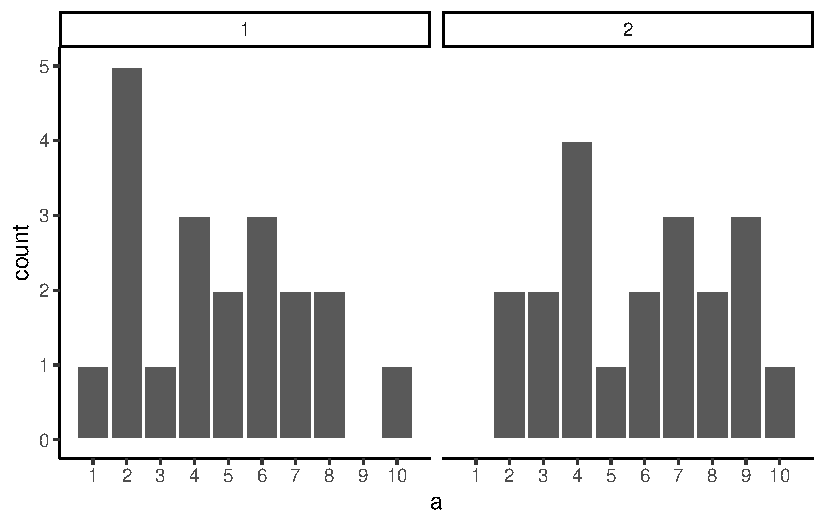
\includegraphics[width=0.75\textwidth,height=\textheight]{05-Foundation_Inference_files/figure-pdf/fig-5whichone-1.pdf}

}

\caption{\label{fig-5whichone}Which of these two samples came from a
uniform distribution?}

\end{figure}

The answer is that they both did. But, neither of them look like they
did.

Can we improve things, and make it easier to see if a sample came from a
uniform distribution? Yes, we can. All we need to do is increase the
\textbf{sample-size}. We will often use the letter \texttt{n} to refer
to sample-size. N is the number of observations in the sample.

So let's increase the number of observations in each sample from 20 to
100. We will again create 10 samples (each with 100 observations), and
make histograms for each of them. All of these samples will be drawn
from the very same uniform distribution. This, means we should expect
each number from 1 to 10 to occur about 10 times in each sample. The
histograms are shown in Figure~\ref{fig-5unifsamp100}.

\begin{figure}

{\centering 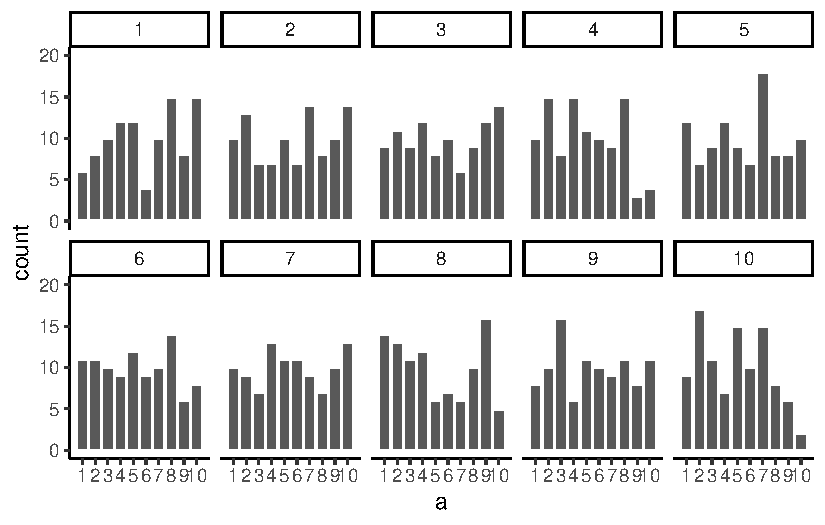
\includegraphics[width=1\textwidth,height=\textheight]{05-Foundation_Inference_files/figure-pdf/fig-5unifsamp100-1.pdf}

}

\caption{\label{fig-5unifsamp100}Histograms for different samples from a
uniform distribution. N = 100 for each sample.}

\end{figure}

Again, most of these histograms don't look very flat, and all of the
bars seem to be going up or down, and they are not exactly at 10 each.
So, we are still dealing with sampling error. It's a pain. It's always
there.

Let's bump up the \(N\) from 100 to 1000 observations per sample. Now we
should expect every number to appear about 100 times each. What happens?

\begin{figure}

{\centering 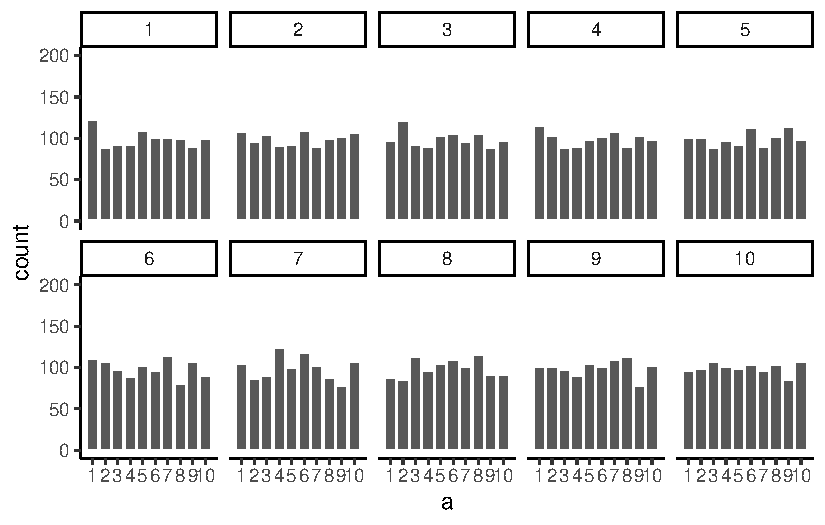
\includegraphics[width=1\textwidth,height=\textheight]{05-Foundation_Inference_files/figure-pdf/fig-5unifsamp1000-1.pdf}

}

\caption{\label{fig-5unifsamp1000}Histograms for different samples from
a uniform distribution. N = 1000 for each sample.}

\end{figure}

Figure~\ref{fig-5unifsamp1000} shows the histograms are starting to
flatten out. The bars are still not perfectly at 100, because there is
still sampling error (there always will be). But, if you found a
histogram that looked flat and knew that the sample contained many
observations, you might be more confident that those numbers came from a
uniform distribution.

Just for fun let's make the samples really big. Say 100,000 observations
per sample. Here, we should expect that each number occurs about 10,000
times each. What happens?

\begin{figure}

{\centering 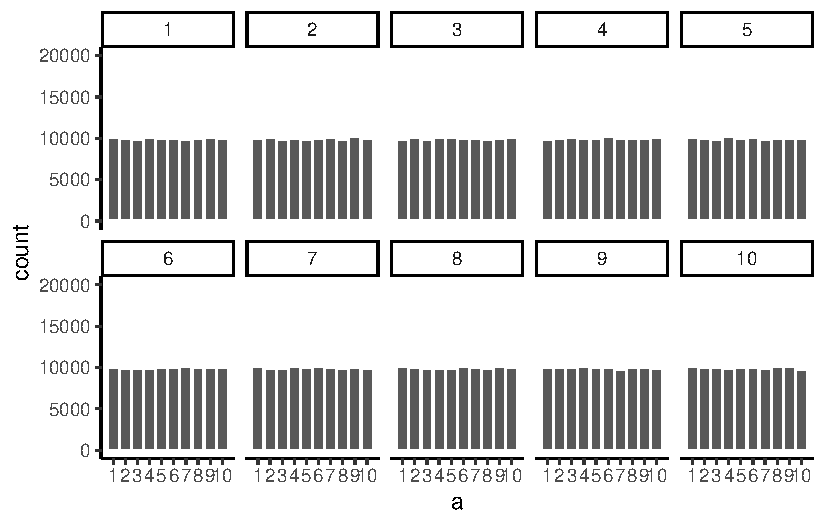
\includegraphics[width=1\textwidth,height=\textheight]{05-Foundation_Inference_files/figure-pdf/fig-5sampunifALOT-1.pdf}

}

\caption{\label{fig-5sampunifALOT}Histograms for different samples from
a uniform distribution. N = 100,000 for each sample.}

\end{figure}

Figure~\ref{fig-5sampunifALOT} shows that the histograms for each sample
are starting to look the same. They all have 100,000 observations, and
this gives chance enough opportunity to equally distribute the numbers,
roughly making sure that they all occur very close to the same amount of
times. As you can see, the bars are all very close to 10,000, which is
where they should be if the sample came from a uniform distribution.

\begin{tcolorbox}[enhanced jigsaw, breakable, colback=white, coltitle=black, toptitle=1mm, rightrule=.15mm, title=\textcolor{quarto-callout-tip-color}{\faLightbulb}\hspace{0.5em}{Pro tip}, opacitybacktitle=0.6, opacityback=0, colframe=quarto-callout-tip-color-frame, leftrule=.75mm, colbacktitle=quarto-callout-tip-color!10!white, arc=.35mm, bottomtitle=1mm, titlerule=0mm, bottomrule=.15mm, toprule=.15mm, left=2mm]

The pattern behind a sample will tend to stabilize as sample-size
increases. Small samples will have all sorts of patterns because of
sampling error (chance).

\end{tcolorbox}

Before getting back to the topic of experiments that we started with,
let's ask two more questions. First, which of the two samples in
Figure~\ref{fig-5whichoneB} do you think came from a uniform
distribution? FYI, each of these samples had 20 observations each.

\begin{figure}

{\centering 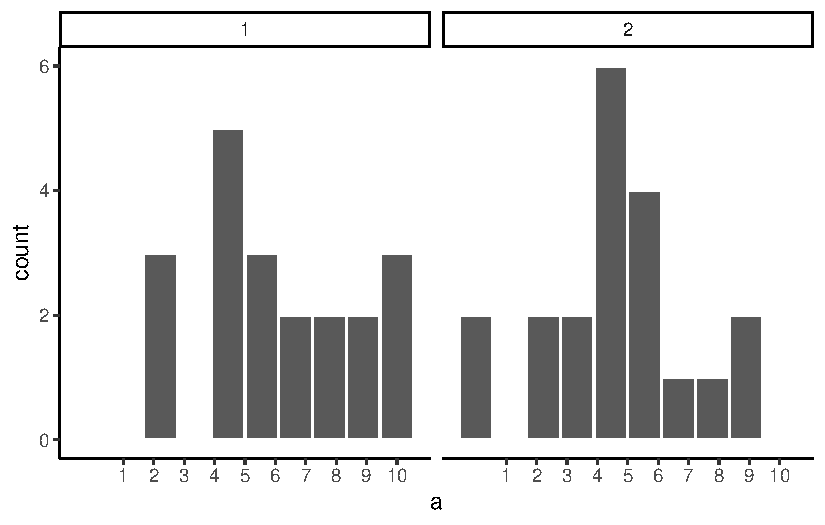
\includegraphics[width=0.75\textwidth,height=\textheight]{05-Foundation_Inference_files/figure-pdf/fig-5whichoneB-1.pdf}

}

\caption{\label{fig-5whichoneB}Which of these samples came from a
uniform distribution?}

\end{figure}

If you are not confident in the answer, this is because \textbf{sampling
error} (randomness) is fuzzing with the histograms.

Here is the very same question, only this time we will take 1,000
observations for each sample. Which histogram in
Figure~\ref{fig-5whichoneC} do you think came from a uniform
distribution, which one did not?

\begin{figure}

{\centering \includegraphics[width=0.75\textwidth,height=\textheight]{05-Foundation_Inference_files/figure-pdf/fig-5whichoneC-1.pdf}

}

\caption{\label{fig-5whichoneC}Which of these samples came from a
uniform distribution?}

\end{figure}

Now that we have increased N, we can see the pattern in each sample
becomes more obvious. The histogram for sample 1 has bars near 100, not
perfectly flat, but it resembles a uniform distribution. The histogram
for sample 2 is not flat looking at all.

Congratulations to Us! We have just made some statistical inferences
without using formulas!

``We did?'' Yes, by looking at our two samples we have inferred that
sample 2 did not come from a uniform distribution. We have also inferred
that sample 1 could have come form a uniform distribution. Fantastic.
These are the same kinds of inferences we will be making for the rest of
the course. We will be looking at some numbers, wondering where they
came from, then we will arrange the numbers in such a way so that we can
make inferences about the kind of distribution they came from. That's
it.

\hypertarget{is-there-a-difference}{%
\section{Is there a difference?}\label{is-there-a-difference}}

Let's get back to experiments. In an experiment we want to know if an
independent variable (our manipulation) causes a change in a dependent
variable (measurement). If this occurs, then we will expect to see some
differences in our measurement as a function of the manipulation.

Consider the light switch example:

\begin{center}\rule{0.5\linewidth}{0.5pt}\end{center}

\textbf{Light Switch Experiment}: You manipulate the switch up
(condition 1 of independent variable), light goes on (measurement). You
manipulate the switch down (condition 2 of independent variable), light
goes off (another measurement). The measurement (light) changes (goes
off and on) as a function of the manipulation (moving switch up or
down).

You can see the change in measurement between the conditions, it is as
obvious as night and day. So, when you conduct a manipulation, and can
see the difference (change) in your measure, you can be pretty confident
that your manipulation is causing the change.

\begin{quote}
note: to be cautious we can say ``something'' about your manipulation is
causing the change, it might not be what you think it is if your
manipulation is very complicated and involves lots of moving parts.
\end{quote}

\begin{center}\rule{0.5\linewidth}{0.5pt}\end{center}

\hypertarget{chance-can-produce-differences}{%
\subsection{Chance can produce
differences}\label{chance-can-produce-differences}}

Do you think random chance can produce the appearance of differences,
even when there really aren't any? I hope so. We have already shown that
the process of sampling numbers from a distribution is a chancy process
that produces different samples. Different samples are different, so
yes, chance can produce differences. This can muck up our interpretation
of experiments.

Let's conduct a fictitious experiment where we expect to find no
differences, because we will manipulate something that shouldn't do
anything. Here's the set-up:

You are the experimenter standing in front of a gumball machine. It is
very big, has thousands of gumballs. 50\% of the gumballs are green, and
50\% are red. You want to find out if picking gumballs with your right
hand vs.~your left hand will cause you to pick more green gumballs.
Plus, you will be blindfolded the entire time. The independent variable
is Hand: right hand vs.~left hand. The dependent variable is the
measurement of the color of each gumball.

You run the experiment as follows. 1) put on blind fold. 2) pick 10
gumballs randomly with left hand, set them aside. 3) pick 10 gumballs
randomly with right hand, set them aside. 4) count the number of green
and red gumballs chosen by your left hand, and count the number of green
and red gumballs chosen by your right hand. Hopefully you will agree
that your hands will not be able to tell the difference between the
gumballs. If you don't agree, we will further stipulate the gumballs are
completely identical in every way except their color, so it would be
impossible to tell them apart using your hands. So, what should happen
in this experiment?

``Umm, maybe you get 5 red gum balls and 5 green balls from your left
hand, and also from your right hand?''. Sort of yes, this is what you
would usually get. But, it is not all that you can get. Here is some
data showing what happened from one pretend experiment:

\begin{longtable}[]{@{}lr@{}}
\toprule\noalign{}
hand & gumball \\
\midrule\noalign{}
\endhead
\bottomrule\noalign{}
\endlastfoot
left & 0 \\
left & 1 \\
left & 1 \\
left & 1 \\
left & 0 \\
left & 0 \\
left & 1 \\
left & 1 \\
left & 0 \\
left & 1 \\
right & 0 \\
right & 0 \\
right & 1 \\
right & 1 \\
right & 1 \\
right & 0 \\
right & 1 \\
right & 0 \\
right & 1 \\
right & 1 \\
\end{longtable}

``What am I looking at here''. This is a long-format table. Each row is
one gumball. The first column tells you what hand was used. The second
column tells you what kind of gumball. We will say 1s stand for green
gum balls, and 0s stand for red gumballs. So, did your left hand cause
you to pick more green gumballs than your right hand?

It would be easier to look at the data using a bar graph
(Figure~\ref{fig-5gumballA}). To keep things simple, we only count the
green gumballs (the other gumballs must be red). So, all we need to do
is sum up the 1s. The 0s won't add anything.

\begin{figure}

{\centering \includegraphics[width=0.75\textwidth,height=\textheight]{05-Foundation_Inference_files/figure-pdf/fig-5gumballA-1.pdf}

}

\caption{\label{fig-5gumballA}Counts of green gumballs picked randomly
by each hand.}

\end{figure}

Oh look, the bars are not the same. One hand picked more green gum balls
than the other. Does this mean that one of your hands secretly knows how
to find green gumballs? No, it's just another case of sampling error,
that thing we call luck or chance. The difference here is caused by
chance, not by the manipulation (which hand you use). \textbf{Major
problem for inference alert}. We run experiments to look for differences
so we can make inferences about whether our manipulations cause change
in our measures. However, this example demonstrates that we can find
differences by chance. How can we know if a difference is real, or just
caused by chance?

\hypertarget{differences-due-to-chance-can-be-simulated}{%
\subsection{Differences due to chance can be
simulated}\label{differences-due-to-chance-can-be-simulated}}

Remember when we showed that chance can produce correlations. We also
showed that chance is restricted in its ability to produce correlations.
For example, chance more often produces weak correlations than strong
correlations. Remember the window of chance? We found out before that
correlations falling outside the window of chance were very unlikely. We
can do the same thing for differences. Let's find out just what chance
can do in our experiment. Once we know what chance is capable of we will
be in a better position to judge whether our manipulation caused a
difference, or whether it could have been chance.

The first thing to do is pretend you conduct the gumball experiment 10
times in a row. This will produce 10 different sets of results.
Figure~\ref{fig-5gumballsims} shows bar graphs for each replication of
the experiment. Now we can look at whether the left hand chose more
green gumballs than red gumballs.

\begin{figure}

{\centering \includegraphics[width=1\textwidth,height=\textheight]{05-Foundation_Inference_files/figure-pdf/fig-5gumballsims-1.pdf}

}

\caption{\label{fig-5gumballsims}10 simulated replications of picking
gumballs. Each replication gives a slightly different answer. Any
difference between the bars is due to chance, or sampling error. This
shows that chance alone can produce differences, just by the act of
sampling.}

\end{figure}

These 10 experiments give us a better look at what chance can do. It
should also mesh well with your expectations. If everything is
determined by chance (as we have made it so), then sometimes your left
hand will choose more green balls, sometimes your right hand will choose
more green gumballs, and sometimes they will choose the same amount of
gumballs. Right? Right.

\hypertarget{chance-makes-some-differences-more-likely-than-others}{%
\section{Chance makes some differences more likely than
others}\label{chance-makes-some-differences-more-likely-than-others}}

OK, we have seen that chance can produce differences here. But, we still
don't have a good idea about what chance usually does and doesn't do.
For example, if we could find the window of opportunity here, we would
be able find out that chance usually does not produce differences of a
certain large size. If we knew what the size was, then if we ran
experiment and our difference was bigger than what chance can do, we
could be confident that chance did not produce our difference.

Let's think about our measure of green balls in terms of a difference.
For example, in each experiment we counted the green balls for the left
and right hand. What we really want to know is if there is a difference
between them. So, we can calculate the \textbf{difference score}. Let's
decide that the difference score = \# of green gumballs in left hand -
\# of green gumballs in right hand. Figure~\ref{fig-5gumballdiffs}
redraws the 10 bar graphs from above; however, now there is only one bar
for each experiment. This bar represents the difference in number of
green gumballs drawn by the left and right hand.

\begin{figure}

{\centering \includegraphics[width=0.75\textwidth,height=\textheight]{05-Foundation_Inference_files/figure-pdf/fig-5gumballdiffs-1.pdf}

}

\caption{\label{fig-5gumballdiffs}A look at the differences between
number of each kind of gumball for the different replications. The
difference should be zero, but sampling error produces non-zero
differences.}

\end{figure}

Missing bars mean that there were an equal number of green gumballs
chosen by the left and right hands (difference score is 0). A positive
value means that more green gumballs were chosen by the left than right
hand. A negative value means that more green gumballs were chosen by the
right than left hand. Note that if we decided (and we get to decide) to
calculate the difference in reverse (right hand - left hand), the signs
of the differences scores would flip around.

We are starting to see more of the differences that chance can produce.
The difference scores are mostly between -2 to +2. We could get an even
better impression by running this pretend experiment 100 times instead
of only 10 times. The results are shown in Figure~\ref{fig-5manydiffs}.

\begin{figure}

{\centering \includegraphics[width=0.75\textwidth,height=\textheight]{05-Foundation_Inference_files/figure-pdf/fig-5manydiffs-1.pdf}

}

\caption{\label{fig-5manydiffs}Replicating the experiment 100 times, and
looking at the differences each time. There are mnay kinds of
differences that chance alone can produce.}

\end{figure}

Ooph, we just ran so many simulated experiments that the x-axis is
unreadable, but it goes from 1 to 100. Each bar represents the
difference of number of green balls chosen randomly by the left or right
hand. Beginning to notice anything? Look at the y-axis, this shows the
size of the difference. Yes, there are lots of bars of different sizes,
this shows us that many kinds of differences do occur by chance.
However, the y-axis is also restricted. It does not go from -10 to +10.
Big differences greater than 5 or -5 don't happen very often.

Now that we have a method for simulating differences due to chance,
let's run 10,000 simulated experiments. But, instead of plotting the
differences in a bar graph for each experiment, how about we look at the
histogram of difference scores. The histogram in
Figure~\ref{fig-5histdiffgumball} provides a clearer picture about which
differences happen most often, and which ones do not. This will be
another window into observing what kinds of differences chance is
capable of producing.

\begin{figure}

{\centering \includegraphics[width=0.75\textwidth,height=\textheight]{05-Foundation_Inference_files/figure-pdf/fig-5histdiffgumball-1.pdf}

}

\caption{\label{fig-5histdiffgumball}A histogram of the differences
obtained by chance over 10,000 replications. The most frequency
difference is 0, which is what we expect by chance. But the differences
can be as large as -10 or +10. Larger differences occur less often by
chance. Chance can't do everything.}

\end{figure}

Our computer simulation allows us to force chance to operate hundreds of
times, each time it produces a difference. We record the difference,
then at the end of the simulation we plot the histogram of the
differences. The histogram begins to show us the where the differences
came from. Remember the idea that numbers come from a distribution, and
the distribution says how often each number occurs. We are looking at
one of these distributions. It is showing us that chance produces some
differences more often than others. First, chance usually produces 0
differences, that's the biggest bar in the middle. Chance also produces
larger differences, but as the differences get larger (positive or
negative), they occur less frequently. The shape of this histogram is
your chance window, it tells you what chance can do, it tells you what
chance usually does, and what it usually does not do.

You can use this chance window to help you make inferences. If you ran
yourself in the gumball experiment and found that your left hand chose 2
more green gumballs than red gumballs, would you conclude that you left
hand was special, and caused you to choose more green gumballs?
Hopefully not. You could look at the chance window and see that
differences of size +2 do happen fairly often by chance alone. You
should not be surprised if you got a +2 difference. However, what if
your left chose 5 more green gumballs than red gumballs. Well, chance
doesn't do this very often, you might think something is up with your
left hand. If you got a whopping 9 more green gumballs than red
gumballs, you might really start to wonder. This is the kind of thing
that could happen (it's possible), but virtually never happens by
chance. When you get things that almost never happen by chance, you can
be more confident that the difference reflects a causal force that is
not chance.

\hypertarget{the-crump-test}{%
\section{The Crump Test}\label{the-crump-test}}

We are going to be doing a lot of inference throughout the rest of this
course. Pretty much all of it will come down to one question. Did chance
produce the differences in my data? We will be talking about experiments
mostly, and in experiments we want to know if our manipulation caused a
difference in our measurement. But, we measure things that have natural
variability, so every time we measure things we will always find a
difference. We want to know if the difference we found (between our
experimental conditions) could have been produced by chance. If chance
is a very unlikely explanation of our observed difference, we will make
the inference that chance did not produce the difference, and that
something about our experimental manipulation did produce the
difference. This is it (for this textbook).

\begin{tcolorbox}[enhanced jigsaw, breakable, colback=white, coltitle=black, toptitle=1mm, rightrule=.15mm, title=\textcolor{quarto-callout-note-color}{\faInfo}\hspace{0.5em}{Note}, opacitybacktitle=0.6, opacityback=0, colframe=quarto-callout-note-color-frame, leftrule=.75mm, colbacktitle=quarto-callout-note-color!10!white, arc=.35mm, bottomtitle=1mm, titlerule=0mm, bottomrule=.15mm, toprule=.15mm, left=2mm]

Statistics is not only about determining whether chance could have
produced a pattern in the observed data. The same tools we are talking
about here can be generalized to ask whether any kind of distribution
could have produced the differences. This allows comparisons between
different models of the data, to see which one was the most likely,
rather than just rejecting the unlikely ones (e.g., chance). But, we'll
leave those advanced topics for another textbook.

\end{tcolorbox}

This chapter is about building intuitions for making these kinds of
inferences about the role of chance in your data. It's not clear to me
what are the best things to say, to build up your intuitions for how to
do statistical inference. So, this chapter tries different things, some
of them standard, and some of them made up. What you are about to read,
is a made up way of doing statistical inference, without using the
jargon that we normally use to talk about it. The goal is to do things
without formulas, and without probabilities, and just work with some
ideas using simulations to see what happens. We will look at what chance
can do, then we will talk about what needs to happen in your data in
order for you to be confident that chance didn't do it.

\hypertarget{intuitive-methods}{%
\subsection{Intuitive methods}\label{intuitive-methods}}

Warning, this is an unofficial statistical test made up by Matt Crump.
It makes sense to him (me), and if it turns out someone else already
made this up, then Crump didn't do his homework, and we will change the
name of this test to it's original author later on. The point of this
test is to show how simple arithmetic operations that you already
understand can be used to create a statistic tool for inference. This
test uses:

\begin{enumerate}
\def\labelenumi{\arabic{enumi}.}
\tightlist
\item
  Sampling numbers randomly from a distribution
\item
  Adding and subtracting
\item
  Division, to find the mean
\item
  Counting
\item
  Graphing and drawing lines
\item
  NO FORMULAS
\end{enumerate}

\hypertarget{part-1-frequency-based-intuition-about-occurrence}{%
\subsection{Part 1: Frequency based intuition about
occurrence}\label{part-1-frequency-based-intuition-about-occurrence}}

\textbf{Question}: How many times does something need to happen for it
to happen a lot? Or, how many times does something need to happen for it
to happen not very much, or even really not at all? Small enough for you
to not worry about it at all happening to you?

Would you go outside everyday if you thought that you would get hit by
lightning 1 out of 10 times? I wouldn't. You'd probably be hit by
lightning more than once per month, you'd be dead pretty quickly. 1 out
of 10 is a lot (to me, maybe not to you, there's no right answer here).

Would you go outside everyday if you thought that you would get hit by
lightning 1 out of every 100 days? Jeez, that's a tough one. What would
I even do? If I went out everyday I'd probably be dead in a year! Maybe
I would go out 2 or 3 times per year, I'm risky like that, but I'd
probably live longer if I stayed at home forever. It would massively
suck.

Would you go outside everyday if you thought you would get hit by
lightning 1 out of every 1000 days? Well, you'd probably be dead in 3-6
years if you did that. Are you a gambler? Maybe go out once per month,
still sucks.

Would you go outside everyday if you thought lightning would get you 1
out every 10,000 days? 10,000 is a bigger number, harder to think about.
It translates to getting hit about once every 27 years. Ya, I'd probably
go out 150 days per year, and keep my fingers crossed.

Would you go outside everyday if you thought lightning would get you 1
out every 100,000 days? How many years is that? It's about 273 years.
With those odds, I'd probably go out all the time and forget about being
hit by lightning. It doesn't happen very often.

The point of considering these questions is to get a sense for yourself
of what happens a lot, and what doesn't happen a lot, and how you would
make important decisions based on what happens a lot and what doesn't.

\hypertarget{part-2-simulating-chance}{%
\subsection{Part 2: Simulating chance}\label{part-2-simulating-chance}}

This next part could happen a bunch of ways, I'll make loads of
assumptions that I won't defend, and I won't claim the Crump test has
problems. I will claim it helps us make an inference about whether
chance could have produced some differences in data. We've already been
introduced to simulating things, so we'll do that again. Here is what we
will do. I am a cognitive psychologist who happens to be measuring X.
Because of prior research in the field, I know that when I measure X, my
samples will tend to have a particular mean and standard deviation.
Let's say the mean is usually 100, and the standard deviation is usually
15. In this case, I don't care about using these numbers as estimates of
the population parameters, I'm just thinking about what my samples
usually look like. What I want to know is how they behave when I sample
them. I want to see what kind of samples happen a lot, and what kind of
samples don't happen a lot. Now, I also live in the real world, and in
the real world when I run experiments to see what changes X, I usually
only have access to some number of participants, who I am very grateful
too, because they participate in my experiments. Let's say I usually can
run 20 subjects in each condition in my experiments. Let's keep the
experiment simple, with two conditions, so I will need 40 total
subjects.

I would like to learn something to help me with inference. One thing I
would like to learn is what the sampling distribution of the sample mean
looks like. This distribution tells me what kinds of mean values happen
a lot, and what kinds don't happen very often. But, I'm actually going
to skip that bit. Because what I'm really interested in is what the
\textbf{sampling distribution of the difference between my sample means}
looks like. After all, I am going to run an experiment with 20 people in
one condition, and 20 people in the other. Then I am going to calculate
the mean for group A, and the mean for group B, and I'm going to look a
the difference. I will probably find a difference, but my question is,
did my manipulation cause this difference, or is this the kind of thing
that happens a lot by chance. If I knew what chance can do, and how
often it produces differences of particular sizes, I could look at the
difference I observed, then look at what chance can do, and then I can
make a decision! If my difference doesn't happen a lot (we'll get to how
much not a lot is in a bit), then I might be willing to believe that my
manipulation caused a difference. If my difference happens all the time
by chance alone, then I wouldn't be inclined to think my manipulation
caused the difference, because it could have been chance.

So, here's what we'll do, even before running the experiment. We'll do a
simulation. We will sample numbers for group A and Group B, then compute
the means for group A and group B, then we will find the difference in
the means between group A and group B. But, we will do one very
important thing. We will pretend that we haven't actually done a
manipulation. If we do this (do nothing, no manipulation that could
cause a difference), then we know that \textbf{only sampling error}
could cause any differences between the mean of group A and group B.
We've eliminated all other causes, only chance is left. By doing this,
we will be able to see exactly what chance can do. More importantly, we
will see the kinds of differences that occur a lot, and the kinds that
don't occur a lot.

Before we do the simulation, we need to answer one question. How much is
a lot? We could pick any number for a lot. I'm going to pick 10,000.
That is a lot. If something happens only 1 times out 10,000, I am
willing to say that is not a lot.

OK, now we have our number, we are going to simulate the possible mean
differences between group A and group B that could arise by chance. We
do this 10,000 times. This gives chance a lot of opportunity to show us
what it does do, and what it does not do.

This is what I did: I sampled 20 numbers into group A, and 20 into group
B. The numbers both came from the same normal distribution, with mean =
100, and standard deviation = 15. Because the samples are coming from
the same distribution, we expect that on average they will be similar
(but we already know that samples differ from one another). Then, I
compute the mean for each sample, and compute the difference between the
means. I save the \textbf{mean difference score}, and end up with 10,000
of them. Then, I draw the histogram in Figure~\ref{fig-5crumptestdiff}.

\begin{figure}

{\centering \includegraphics[width=0.75\textwidth,height=\textheight]{05-Foundation_Inference_files/figure-pdf/fig-5crumptestdiff-1.pdf}

}

\caption{\label{fig-5crumptestdiff}Histogram of mean differences arising
by chance.}

\end{figure}

\begin{tcolorbox}[enhanced jigsaw, breakable, colback=white, coltitle=black, toptitle=1mm, rightrule=.15mm, title=\textcolor{quarto-callout-note-color}{\faInfo}\hspace{0.5em}{Note}, opacitybacktitle=0.6, opacityback=0, colframe=quarto-callout-note-color-frame, leftrule=.75mm, colbacktitle=quarto-callout-note-color!10!white, arc=.35mm, bottomtitle=1mm, titlerule=0mm, bottomrule=.15mm, toprule=.15mm, left=2mm]

Of course, we might recognize that chance could do a difference greater
than 15. We just didn't give it the opportunity. We only ran the
simulation 10,000 times. If we ran it a million times, maybe a
difference greater than 15 or even 20 would happen a couple times. If we
ran it a bazillion gazillion times, maybe a difference greater than 30
would happen a couple times. If we go out to infinity, then chance might
produce all sorts of bigger differences once in a while. But, we've
already decided that 1/10,000 is not a lot. So things that happen 0 out
of 10,000 times, like differences greater than 15, are considered to be
extremely unlikely.

\end{tcolorbox}

Now we can see what chance can do to the size of our mean difference.
The x-axis shows the size of the mean difference. We took our samples
from the sample distribution, so the difference between them should
usually be 0, and that's what we see in the histogram.

Pause for a second. Why should the mean differences usually be zero,
wasn't the population mean = 100, shouldn't they be around 100? No.~The
mean of group A will tend to be around 100, and the mean of group B will
tend be around 100. So, the difference score will tend to be 100-100 =
0. That is why we expect a mean difference of zero when the samples are
drawn from the same population.

So, differences near zero happen the most, that's good, that's what we
expect. Bigger or smaller differences happen increasingly less often.
Differences greater than 15 or -15 never happen at all. For our
purposes, it looks like chance only produces differences between -15 to
15.

OK, let's ask a couple simple questions. What was the biggest negative
number that occurred in the simulation? We'll use R for this. All of the
10,000 difference scores are stored in a variable I made called
\texttt{difference}. If we want to find the minimum value, we use the
\texttt{min} function. Here's the result.

\begin{Shaded}
\begin{Highlighting}[]
\FunctionTok{min}\NormalTok{(difference)}
\CommentTok{\#\textgreater{} [1] {-}18.00152}
\end{Highlighting}
\end{Shaded}

OK, so what was the biggest positive number that occurred? Let's use the
\texttt{max} function to find out. It finds the biggest (maximum) value
in the variable. FYI, we've just computed the range, the minimum and
maximum numbers in the data. Remember we learned that before. Anyway,
here's the max.

\begin{Shaded}
\begin{Highlighting}[]
\FunctionTok{max}\NormalTok{(difference)}
\CommentTok{\#\textgreater{} [1] 18.57387}
\end{Highlighting}
\end{Shaded}

Both of these extreme values only occurred once. Those values were so
rare we couldn't even see them on the histogram, the bar was so small.
Also, these biggest negative and positive numbers are pretty much the
same size if you ignore their sign, which makes sense because the
distribution looks roughly symmetrical.

So, what can we say about these two numbers for the min and max? We can
say the min happens 1 times out of 10,000. We can say the max happens 1
times out of 10,000. Is that a lot of times? Not to me. It's not a lot.

So, how often does a difference of 30 (much larger larger than the max)
occur out of 10,000. We really can't say, 30s didn't occur in the
simulation. Going with what we got, we say 0 out of 10,000. That's
never.

We're about to move into part three, which involves drawing decision
lines and talking about them. The really important part about part 3 is
this. What would you say if you ran this experiment once, and found a
mean difference of 30? I would say it happens 0 times of out 10,000 by
chance. I would say chance did not produce my difference of 30. That's
what I would say. We're going to expand upon this right now.

\hypertarget{part-3-judgment-and-decision-making}{%
\subsection{Part 3: Judgment and
Decision-making}\label{part-3-judgment-and-decision-making}}

Remember, we haven't even conducted an experiment. We're just simulating
what could happen if we did conduct an experiment. We made a histogram.
We can see that chance produces some differences more than others, and
that chance never produced really big differences. What should we do
with this information?

What we are going to do is talk about judgment and decision making. What
kind of judgment and decision making? Well, when you finally do run an
experiment, you will get two means for group A and B, and then you will
need to make some judgments, and perhaps even a decision, if you are so
inclined. You will need to judge whether chance (sampling error) could
have produced the difference you observed. If you judge that it did it
not, you might make the decision to tell people that your experimental
manipulation actually works. If you judge that it could have been
chance, you might make a different decision. These are important
decisions for researchers. Their careers can depend on them. Also, their
decisions matter for the public. Nobody wants to hear fake news from the
media about scientific findings.

So, what we are doing is preparing to make those judgments. We are going
to draw up a plan, before we even see the data, for how we will make
judgments and decisions about what we find. This kind of planning is
extremely important, because we discuss in part 4, that your planning
can help you design an even better experiment than the one you might
have been intending to run. This kind of planning can also be used to
interpret other people's results, as a way of double-checking checking
whether you believe those results are plausible.

The thing about judgement and decision making is that reasonable people
disagree about how to do it, unreasonable people really disagree about
it, and statisticians and researchers disagree about how to do it. I
will propose some things that people will disagree with. That's OK,
these things still make sense. And, the disagreeable things point to
important problems that are very real for any ``real'' statistical
inference test.

Let's talk about some objective facts from our simulation of 10,000
things that we definitely know to be true. For example, we can draw some
lines on the graph, and label some different regions. We'll talk about
two kinds of regions.

\begin{enumerate}
\def\labelenumi{\arabic{enumi}.}
\tightlist
\item
  Region of chance. Chance did it. Chance could have done it
\item
  Region of not chance. Chance didn't do it. Chance couldn't have done
  it.
\end{enumerate}

The regions are defined by the minimum value and the maximum value.
Chance never produced a smaller or bigger number. The region inside the
range is what chance did do, and the the region outside the range on
both sides is what chance never did. It looks like
Figure~\ref{fig-5crumpdecision}:

\begin{figure}

{\centering \includegraphics[width=0.75\textwidth,height=\textheight]{05-Foundation_Inference_files/figure-pdf/fig-5crumpdecision-1.pdf}

}

\caption{\label{fig-5crumpdecision}Applying decision boundaries to the
histogrm of mean differences. The boundaries identify what differences
chance did or did not produce in the simulation.}

\end{figure}

We have just drawn some lines, and shaded some regions, and made one
plan we could use to make decisions. How would the decisions work. Let's
say you ran the experiment and found a mean difference between groups A
and B of 25. Where is 25 in the figure? It's in the green part. What
does the green part say? NOT CHANCE. What does this mean. It means
chance never made a difference of 25. It did that 0 out of 10,000 times.
If we found a difference of 25, perhaps we could confidently conclude
that chance did not cause the difference. If I found a difference of 25
with this kind of data, I'd be pretty confident chance did not cause the
difference; and, I would give myself license to consider that my
experimental manipulation may be causing the difference.

What about a difference of +10? That's in the red part, where chance
lives. Chance could have done a difference of +10 because we can see
that it did do that sometimes. The red part is the window of what chance
did in our simulation. Anything inside the window could have been a
difference caused by chance. If I found a difference of +10, I'd say,
``ya, it coulda been chance.'' I would also be less confident that the
difference was only caused by my experimental manipulation.

Statistical inference could be this easy. The number you get from your
experiment could be in the chance window (then you can't rule out chance
as a cause), or it could be outside the chance window (then you can rule
out chance). Case closed. Let's all go home.

\hypertarget{grey-areas}{%
\subsubsection{Grey areas}\label{grey-areas}}

So what's the problem? Depending on who you are, and what kinds of risks
you're willing to take, there might not be a problem. But, if you are
just even a little bit risky then there is a problem that makes clear
judgments about the role of chance difficult. We would like to say
chance did or did not cause our difference. But, we're really always in
the position of admitting that it could have sometimes, or wouldn't have
most times. These are wishy washy statements, they are in between yes or
no. That's OK. Grey is a color too, let's give grey some respect.

``What grey areas are you talking about?, I only see red or green, am I
grey blind?''. Let's look at where some grey areas might be. I say might
be, because people disagree about where the grey is. People have
different comfort levels with grey. Figure~\ref{fig-5crumpuncertainty}
shows my opinion on grey areas.

\begin{figure}

{\centering \includegraphics[width=0.75\textwidth,height=\textheight]{05-Foundation_Inference_files/figure-pdf/fig-5crumpuncertainty-1.pdf}

}

\caption{\label{fig-5crumpuncertainty}The question marks refer to an
area where you have some uncertainty. Differences inside the question
mark region do not happen very often by chance. When you find
differences of these sizes, should you reject the idea that chance
caused your difference? You will always have some uncertainty associated
with this decision because it is clear that chance could have caused the
difference. But, chance usually does not produce differences of these
sizes.}

\end{figure}

I made two grey areas, and they are reddish grey, because we are still
in the chance window. There are question marks (?) in the grey areas.
Why? The question marks reflect some uncertainty that we have about
those particular differences. For example, if you found a difference
that was in a grey area, say a 15. 15 is less than the maximum, which
means chance did create differences of around 15. But, differences of 15
don't happen very often.

What can you conclude or say about this 15 you found? Can you say
without a doubt that chance did not produce the difference? Of course
not, you know that chance could have. Still, it's one of those things
that doesn't happen a lot. That makes chance an unlikely explanation.
Instead of thinking that chance did it, you might be willing to take a
risk and say that your experimental manipulation caused the difference.
You'd be making a bet that it wasn't chance\ldots but, could be a safe
bet, since you know the odds are in your favor.

You might be thinking that your grey areas aren't the same as the ones
I've drawn. Maybe you want to be more conservative, and make them
smaller. Or, maybe you're more risky, and would make them bigger. Or,
maybe you'd add some grey area going in a little bit to the green area
(after all, chance could probably produce some bigger differences
sometimes, and to avoid those you would have to make the grey area go a
bit into the green area).

Another thing to think about is your decision policy. What will you do,
when your observed difference is in your grey area? Will you always make
the same decision about the role of chance? Or, will you sometimes
flip-flop depending on how you feel. Perhaps, you think that there
shouldn't be a strict policy, and that you should accept some level of
uncertainty. The difference you found could be a real one, or it might
not. There's uncertainty, hard to avoid that.

So let's illustrate one more kind of strategy for making decisions. We
just talked about one that had some lines, and some regions. This makes
it seem like a binary choice: we can either rule out, or not rule out
the role of chance. Another perspective is that everything is a
different shade of grey, like in Figure~\ref{fig-5crumpshade}.

\begin{figure}

{\centering \includegraphics[width=0.75\textwidth,height=\textheight]{05-Foundation_Inference_files/figure-pdf/fig-5crumpshade-1.pdf}

}

\caption{\label{fig-5crumpshade}The shading of the blue bars indicates
levels of confidence in whether a difference could have been produced by
chance. Darker bars represent increased confidence that the difference
was not produced by chance. Bars get darker as the mean difference
increases in absolute value.}

\end{figure}

OK, so I made it shades of blue (because it was easier in R). Now we can
see two decision plans at the same time. Notice that as the bars get
shorter, they also get become a darker stronger blue. The color can be
used as a guide for your confidence. That is, your confidence in the
belief that your manipulation caused the difference rather than chance.
If you found a difference near a really dark bar, those don't happen
often by chance, so you might be really confident that chance didn't do
it. If you find a difference near a slightly lighter blue bar, you might
be slightly less confident. That is all. You run your experiment, you
get your data, then you have some amount of confidence that it wasn't
produced by chance. This way of thinking is elaborated to very
interesting degrees in the Bayesian world of statistics. We don't wade
too much into that, but mention it a little bit here and there. It's
worth knowing it's out there.

\hypertarget{making-decisions-and-being-wrong}{%
\subsubsection{Making decisions and being
wrong}\label{making-decisions-and-being-wrong}}

No matter how you plan to make decisions about your data, you will
always be prone to making some mistakes. You might call one finding
real, when in fact it was caused by chance. This is called a
\textbf{type I} error, or a false positive. You might ignore one
finding, calling it chance, when in fact it wasn't chance (even though
it was in the window). This is called a \textbf{type II} error, or a
false negative.

How you make decisions can influence how often you make errors over
time. If you are a researcher, you will run lots of experiments, and you
will make some amount of mistakes over time. If you do something like
the very strict method of only accepting results as real when they are
in the ``no chance'' zone, then you won't make many type I errors.
Pretty much all of your result will be real. But, you'll also make type
II errors, because you will miss things real things that your decision
criteria says are due to chance. The opposite also holds. If you are
willing to be more liberal, and accept results in the grey as real, then
you will make more type I errors, but you won't make as many type II
errors. Under the decision strategy of using these cutoff regions for
decision-making there is a necessary trade-off. The Bayesian view get's
around this a little bit. Bayesians talk about updating their beliefs
and confidence over time. In that view, all you ever have is some level
of confidence about whether something is real, and by running more
experiments you can increase or decrease your level of confidence. This,
in some fashion, avoids some trade-off between type I and type II
errors.

Regardless, there is another way to reduce type I and type II errors,
and to increase your confidence in your results, even before you do the
experiment. It's called ``knowing how to design a good experiment''.

\hypertarget{part-4-experiment-design}{%
\subsection{Part 4: Experiment Design}\label{part-4-experiment-design}}

We've seen what chance can do. Now, let's venture into an experiment. We
make a change between ecosystems A and B, gather the data, assess the
average outcomes, and then observe the variance. Then we keep our
fingers crossed, hoping that the variance is significant enough to be
beyond natural fluctuations. Yes, nature keeps us guessing.

Here's the catch, we aren't always certain about the magnitude of our
environmental interventions. So, even if an intervention induces a
change, pinning down its exact magnitude can be challenging. And that's
the essence of our experiment. Many interventions in Environmental
Science might not cause large-scale shifts. This poses a challenge in
identifying these subtle, yet potentially crucial, environmental
effects. In a hypothetical scenario, introducing a certain pollinator
species might influence plant growth, but to what extent? If the
difference is marginal, differentiating between natural variation and
the effect of our intervention becomes tricky. Let's say our
intervention involves introducing shade in one ecosystem versus none in
the other. While shade can influence plant growth, if the effect is only
marginal, it becomes hard to ascertain if it wasn't just a natural
occurrence. And, it's not straightforward to intensify the shading to
amplify its impact, without risking other unintended consequences.

EXPERIMENT DESIGN TO THE RESCUE! Newsflash, it is often possible to
change how you run your experiment so that it is \textbf{more sensitive}
to smaller effects. How do you think we can do this? Here is a hint.
It's the stuff you learned about the sampling distribution of the sample
mean, and the role of sample-size. What happens to the sampling
distribution of the sample mean when N (sample size)? The distribution
gets narrower and narrower, and starts to look the a single number (the
hypothetical mean of the hypothetical population). That's great. If you
switch to thinking about mean difference scores, like the distribution
we created in this test, what do you think will happen to that
distribution as we increase N? It will will also shrink. As we increase
N to infinity, it will shrink to 0. Which means that, when N is
infinity, chance never produces any differences at all. We can use this.

For example, we could run our experiment with 20 subjects in each group.
Or, we could decide to invest more time and run 40 subjects in each
group, or 80, or 150. When you are the experimenter, you get to decide
the design. These decisions matter big time. Basically, the more
subjects you have, the more sensitive your experiment. With bigger N,
you will be able to reliably detect smaller mean differences, and be
able to confidently conclude that chance did not produce those small
effects.

Check out the histograms in Figure~\ref{fig-5sampleDistNormal}. This is
the same simulation as before, but with four different sample-sizes: 20,
40, 80, 160. We are doubling our sample-size across each simulation just
to see what happens to the width of the chance window.

\begin{figure}

{\centering \includegraphics[width=0.75\textwidth,height=\textheight]{05-Foundation_Inference_files/figure-pdf/fig-5sampleDistNormal-1.pdf}

}

\caption{\label{fig-5sampleDistNormal}The range or width of the
differences produced by chance shrinks as sample-size increases.}

\end{figure}

There you have it. The \textbf{sampling distribution of the mean
differences} shrinks toward 0 as sample-size increases. This means if
you run an experiment with a larger sample-size, you will be able to
detect smaller mean differences, and be confident they aren't due to
chance. Table~\ref{tbl-5minmax} contains the minimum and maximum values
that chance produced across the four sample-sizes:

\hypertarget{tbl-5minmax}{}
\begin{longtable}[]{@{}rrr@{}}
\caption{\label{tbl-5minmax}The smallest and largest mean differences
produced by chance as a function of sample-size.}\tabularnewline
\toprule\noalign{}
sample\_size & smallest & largest \\
\midrule\noalign{}
\endfirsthead
\toprule\noalign{}
sample\_size & smallest & largest \\
\midrule\noalign{}
\endhead
\bottomrule\noalign{}
\endlastfoot
20 & -27.80689 & 24.88639 \\
40 & -16.58451 & 17.34902 \\
80 & -13.72506 & 11.77566 \\
160 & -10.62335 & 10.99505 \\
\end{longtable}

The table shows the range of chance behavior is very wider for smaller N
and narrower for larger N. Consider what this narrowing means for your
experiment design. For example, one aspect of the design is the choice
of sample size, N, or in a psychology experiment the number of
participants.

If it turns out your manipulation will cause a difference of +11, then
what should you do? Run an experiment with N = 20 people? I hope not. If
you did that, you could get a mean difference of +11 fairly often by
chance. However, if you ran the experiment with 160 people, then you
would definitely be able to say that +11 was not due to chance, it would
be outside the range of what chance can do. You could even consider
running the experiment with 80 subjects. A +11 there wouldn't happen
often by chance, and you'd be cost-effective, spending less time on the
experiment.

The point is: \textbf{the design of the experiment determines the sizes
of the effects it can detect}. If you want to detect a small effect.
Make your sample size bigger. It's really important to say this is not
the only thing you can do. You can also make your cell-sizes bigger. For
example, often times we take several measurements from a single subject.
The more measurements you take (cell-size), the more stable your
estimate of the subject's mean. We discuss these issues more later. You
can also make a stronger manipulation, when possible.

\hypertarget{part-5-i-have-the-power}{%
\subsection{Part 5: I have the power}\label{part-5-i-have-the-power}}

\begin{quote}
By the power of greyskull, I HAVE THE POWER - He-man
\end{quote}

The last topic in this section is called \textbf{power}. Later we will
define power in terms of some particular ideas about statistical
inference. Here, we will just talk about the big idea. And, we'll show
how to make sure your design has 100\% power. Because, why not. Why run
a design that doesn't have the power?

The big idea behind power is the concept of sensitivity. The concept of
sensitivity assumes that there is something to be sensitive to. That is,
there is some real difference that can be measured. So, the question is,
how sensitive is your experiment? We've already seen that the number of
subjects (sample-size), changes the sensitivity of the design. More
subjects = more sensitivity to smaller effects.

Let's take a look at one more plot. What we will do is simulate a
measure of sensitivity across a whole bunch of sample sizes, from 10 to
300. We'll do this in steps of 10. For each simulation, we'll compute
the mean differences as we have done. But, rather than showing the
histogram, we'll just compute the smallest value and the largest value.
This is a pretty good measure of the outer reach of chance. Then we'll
plot those values as a function of sample size and see what we've got.

\begin{figure}

{\centering \includegraphics[width=0.75\textwidth,height=\textheight]{05-Foundation_Inference_files/figure-pdf/fig-5crumpminmax-1.pdf}

}

\caption{\label{fig-5crumpminmax}A graph of the maximum and minimum mean
differences produced by chance as a function of sample-size. The range
narrows as sample-size increases showing that chance alone produces a
smaller range of mean differences as sample-size increases.}

\end{figure}

Figure~\ref{fig-5crumpminmax} shows a reasonably precise window of
sensitivity as a function of sample size. For each sample size, we can
see the maximum difference that chance produced and the minimum
difference. In those simulations, chance never produced bigger or
smaller differences. So, each design is sensitive to any difference that
is underneath the bottom line, or above the top line.

Here's another way of putting it. Which of the sample sizes will be
sensitive to a difference of +10 or -10. That is, if a difference of +10
or -10 was observed, then we could very confidently say that the
difference was not due to chance, because according to these
simulations, chance never produced differences that big. To help us see
which ones are sensitive, Figure~\ref{fig-5crumpredline} draws
horizontal lines at -10 and +10.

\begin{figure}

{\centering \includegraphics[width=0.75\textwidth,height=\textheight]{05-Foundation_Inference_files/figure-pdf/fig-5crumpredline-1.pdf}

}

\caption{\label{fig-5crumpredline}The red line represents the size of a
mean difference that a researcher may be interested in detecting. All of
the dots outside (above or below) the red line represent designs with
small sample-sizes. When a difference of 10 occurs for these designs, we
can rule out chance with confidence. The dots between the red lines
represent designs with larger sample-sizes. These designs never produce
differences as large as 10, so when those differences occur, we can be
confident chance did not produce them.}

\end{figure}

Based on visual guesstimation, the designs with sample-size
\textgreater= 100 are all sensitive to real differences of 10. Designs
with sample-size \textgreater{} 100 all failed to produce extreme
differences outside of the red lines by chance alone. If these designs
were used, and if an effect of 10 or larger was observed, then we could
be confident that chance alone did not produce the effect. Designing
your experiment so that you know it is sensitive to the thing you are
looking for is the big idea behind power.

\hypertarget{summary-of-crump-test}{%
\subsection{Summary of Crump Test}\label{summary-of-crump-test}}

What did we learn from this so-called fake Crump test that nobody uses?
Well, we learned the basics of what we'll be doing moving forward. And,
we did it all without any hard math or formulas. We sampled numbers, we
computed means, we subtracted means between experimental conditions,
then we repeated that process many times and counted up the mean
differences and put them in a histogram. This showed us what chance do
in an experiment. Then, we discussed how to make decisions around these
facts. And, we showed how we can control the role of chance just by
changing things like sample size.

\hypertarget{the-randomization-test-permutation-test}{%
\section{The randomization test (permutation
test)}\label{the-randomization-test-permutation-test}}

Welcome to the first official inferential statistic in this textbook. Up
till now we have been building some intuitions for you. Next, we will
get slightly more formal and show you how we can use random chance to
tell us whether our experimental finding was likely due to chance or
not. We do this with something called a randomization test. The ideas
behind the randomization test are the very same ideas behind the rest of
the inferential statistics that we will talk about in later chapters.
And, surprise, we have already talked about all of the major ideas
already. Now, we will just put the ideas together, and give them the
name \textbf{randomization test}.

Here's the big idea. When you run an experiment and collect some data
you get to find out what happened that one time. But, because you ran
the experiment only once, you don't get to find out what \textbf{could
have happened}. The randomization test is a way of finding out what
\textbf{could have happened}. And, once you know that, you can compare
\textbf{what did happen} in your experiment, with \textbf{what could
have happened}.

\hypertarget{pretend-example-does-chewing-gum-improve-your-grades}{%
\subsection{Pretend example does chewing gum improve your
grades?}\label{pretend-example-does-chewing-gum-improve-your-grades}}

Let's say you run an experiment to find out if chewing gum causes
students to get better grades on statistics exams. You randomly assign
20 students to the chewing gum condition, and 20 different students to
the no-chewing gum condition. Then, you give everybody statistics tests
and measure their grades. If chewing gum causes better grades, then the
chewing gum group should have higher grades on average than the group
who did not chew gum.

Let's say the data looked like this:

\begin{longtable}[]{@{}lll@{}}
\toprule\noalign{}
student & gum & no\_gum \\
\midrule\noalign{}
\endhead
\bottomrule\noalign{}
\endlastfoot
1 & 88 & 44 \\
2 & 77 & 62 \\
3 & 91 & 43 \\
4 & 79 & 46 \\
5 & 81 & 70 \\
6 & 95 & 41 \\
7 & 99 & 56 \\
8 & 79 & 70 \\
9 & 84 & 74 \\
10 & 91 & 61 \\
11 & 80 & 62 \\
12 & 93 & 46 \\
13 & 94 & 83 \\
14 & 99 & 43 \\
15 & 100 & 71 \\
16 & 94 & 58 \\
17 & 94 & 80 \\
18 & 95 & 78 \\
19 & 81 & 42 \\
20 & 81 & 84 \\
Sums & 1775 & 1214 \\
Means & 88.75 & 60.7 \\
\end{longtable}

So, did the students chewing gum do better than the students who didn't
chew gum? Look at the mean test performance at the bottom of the table.
The mean for students chewing gum was 88.75, and the mean for students
who did not chew gum was 60.7. Just looking at the means, it looks like
chewing gum worked!

``STOP THE PRESSES, this is silly''. We already know this is silly
because we are making pretend data. But, even if this was real data, you
might think, ``Chewing gum won't do anything, this difference could have
been caused by chance, I mean, maybe the better students just happened
to be put into the chewing group, so because of that their grades were
higher, chewing gum didn't do anything\ldots{}''. We agree. But, let's
take a closer look. We already know how the data come out. What we want
to know is how they could have come out, what are all the possibilities?

For example, the data would have come out a bit different if we happened
to have put some of the students from the gum group into the no gum
group, and vice versa. Think of all the ways you could have assigned the
40 students into two groups, there are lots of ways. And, the means for
each group would turn out differently depending on how the students are
assigned to each group.

Practically speaking, it's not possible to run the experiment every
possible way, that would take too long. But, we can nevertheless
estimate how all of those experiments might have turned out using
simulation.

Here's the idea. We will take the 40 measurements (exam scores) that we
found for all the students. Then we will randomly take 20 of them and
pretend they were in the gum group, and we'll take the remaining 20 and
pretend they were in the no gum group. Then we can compute the means
again to find out what would have happened. We can keep doing this over
and over again. Every time computing what happened in that version of
the experiment.

\hypertarget{doing-the-randomization}{%
\subsubsection{Doing the randomization}\label{doing-the-randomization}}

Before we do that, let's show how the randomization part works. We'll
use fewer numbers to make the process easier to look at. Here are the
first 5 exam scores for students in both groups.

\begin{longtable}[]{@{}lll@{}}
\toprule\noalign{}
student & gum & no\_gum \\
\midrule\noalign{}
\endhead
\bottomrule\noalign{}
\endlastfoot
1 & 88 & 44 \\
2 & 77 & 62 \\
3 & 91 & 43 \\
4 & 79 & 46 \\
5 & 81 & 70 \\
Sums & 416 & 265 \\
Means & 83.2 & 53 \\
\end{longtable}

Things could have turned out differently if some of the subjects in the
gum group were switched with the subjects in the no gum group. Here's
how we can do some random switching. We will do this using R.

\begin{Shaded}
\begin{Highlighting}[]
\NormalTok{all\_scores       }\OtherTok{\textless{}{-}} \FunctionTok{c}\NormalTok{(gum[}\DecValTok{1}\SpecialCharTok{:}\DecValTok{5}\NormalTok{],no\_gum[}\DecValTok{1}\SpecialCharTok{:}\DecValTok{5}\NormalTok{])}
\NormalTok{randomize\_scores }\OtherTok{\textless{}{-}} \FunctionTok{sample}\NormalTok{(all\_scores)}
\NormalTok{new\_gum          }\OtherTok{\textless{}{-}}\NormalTok{ randomize\_scores[}\DecValTok{1}\SpecialCharTok{:}\DecValTok{5}\NormalTok{]}
\NormalTok{new\_no\_gum       }\OtherTok{\textless{}{-}}\NormalTok{ randomize\_scores[}\DecValTok{6}\SpecialCharTok{:}\DecValTok{10}\NormalTok{]}
\FunctionTok{print}\NormalTok{(new\_gum)}
\CommentTok{\#\textgreater{} [1] 70 81 79 62 77}
\FunctionTok{print}\NormalTok{(new\_no\_gum)}
\CommentTok{\#\textgreater{} [1] 44 46 88 43 91}
\end{Highlighting}
\end{Shaded}

We have taken the first 5 numbers from the original data, and put them
all into a variable called \texttt{all\_scores}. Then we use the
\texttt{sample} function in R to shuffle the scores. Finally, we take
the first 5 scores from the shuffled numbers and put them into a new
variable called \texttt{new\_gum}. Then, we put the last five scores
into the variable \texttt{new\_no\_gum}. Then we printed them, so we can
see them.

If we do this a couple of times and put them in a table, we can indeed
see that the means for gum and no gum would be different if the subjects
were shuffled around. Check it out:

\begin{longtable}[]{@{}lllllll@{}}
\toprule\noalign{}
student & gum & no\_gum & gum2 & no\_gum2 & gum3 & no\_gum3 \\
\midrule\noalign{}
\endhead
\bottomrule\noalign{}
\endlastfoot
1 & 88 & 44 & 70 & 62 & 43 & 91 \\
2 & 77 & 62 & 44 & 81 & 88 & 70 \\
3 & 91 & 43 & 88 & 77 & 62 & 46 \\
4 & 79 & 46 & 91 & 43 & 77 & 44 \\
5 & 81 & 70 & 79 & 46 & 81 & 79 \\
Sums & 416 & 265 & 372 & 309 & 351 & 330 \\
Means & 83.2 & 53 & 74.4 & 61.8 & 70.2 & 66 \\
\end{longtable}

\hypertarget{simulating-the-mean-differences-across-the-different-randomizations}{%
\subsubsection{Simulating the mean differences across the different
randomizations}\label{simulating-the-mean-differences-across-the-different-randomizations}}

In our pretend experiment we found that the mean for students chewing
gum was 88.75, and the mean for students who did not chew gum was 60.7.
The mean difference (gum - no gum) was 28.05. This is a pretty big
difference. This is \textbf{what did happen}. But, \textbf{what could
have happened}? If we tried out all of the experiments where different
subjects were switched around, what does the distribution of the
possible mean differences look like? Let's find out. This is what the
randomization test is all about.

When we do our randomization test we will measure the mean difference in
exam scores between the gum group and the no gum group. Every time we
randomize we will save the mean difference.

Let's look at a short animation of what is happening in the
randomization test. \textbf{?@fig-5randtest} shows data from a different
fake experiment, but the principles are the same. We'll return to the
gum no gum experiment after the animation. The animation is showing
three important things. First, the purple dots show the mean scores in
two groups (didn't study vs study). It looks like there is a difference,
as 1 dot is lower than the other. We want to know if chance could
produce a difference this big. At the beginning of the animation, the
light green and red dots show the individual scores from each of 10
subjects in the design (the purple dots are the means of these original
scores). Now, during the randomizations, we randomly shuffle the
original scores between the groups. You can see this happening
throughout the animation, as the green and red dots appear in different
random combinations. The moving yellow dots show you the new means for
each group after the randomization. The differences between the yellow
dots show you the range of differences that chance could produce.

We are engaging in some visual statistical inference. By looking at the
range of motion of the yellow dots, we are watching what kind of
differences chance can produce. In this animation, the purple dots,
representing the original difference, are generally outside of the range
of chance. The yellow dots don't move past the purple dots, as a result
chance is an unlikely explanation of the difference.

If the purple dots were inside the range of the yellow dots, then when
would know that chance is capable of producing the difference we
observed, and that it does so fairly often. As a result, we should not
conclude the manipulation caused the difference, because it could have
easily occurred by chance.

Let's return to the gum example. After we randomize our scores many
times, and computed the new means, and the mean differences, we will
have loads of mean differences to look at, which we can plot in a
histogram. The histogram gives a picture of \textbf{what could have
happened}. Then, we can compare \textbf{what did happen} with
\textbf{what could have happened}.

Here's the histogram of the mean differences from the randomization
test. For this simulation, we randomized the results from the original
experiment 1000 times. This is what could have happened. The blue line
in Figure~\ref{fig-5randhist} shows where the observed difference lies
on the x-axis.

\begin{figure}

{\centering \includegraphics[width=0.75\textwidth,height=\textheight]{05-Foundation_Inference_files/figure-pdf/fig-5randhist-1.pdf}

}

\caption{\label{fig-5randhist}A histogram of simulated mean differences
for a randomization test}

\end{figure}

What do you think? Could the difference represented by the blue line
have been caused by chance? My answer is probably not. The histogram
shows us the window of chance. The blue line is not inside the window.
This means we can be pretty confident that the difference we observed
was not due to chance.

We are looking at another window of chance. We are seeing a histogram of
the kinds of mean differences that could have occurred in our
experiment, if we had assigned our subjects to the gum and no gum groups
differently. As you can see, the mean differences range from negative to
positive. The most frequent difference is 0. Also, the distribution
appears to be symmetrical about zero, which shows we had roughly same
the chances of getting a positive or negative difference. Also, notice
that as the differences get larger (in the positive or negative
direction, they become less frequent). The blue line shows us
\textbf{the observed difference}, this is the one we found in our fake
experiment. Where is it? It's way out to the right. It is is well
outside the histogram. In other words, when we look at \textbf{what
could have happened}, we see that \textbf{what did happen} doesn't occur
very often.

IMPORTANT: In this case, when we speak of \textbf{what could have
happened}. We are talking about what could have happened \textbf{by
chance}. When we compare what did happen to what chance could have done,
we can get a better idea of whether our result was caused by chance.

\begin{center}\rule{0.5\linewidth}{0.5pt}\end{center}

OK, let's pretend we got a much smaller mean difference when we first
ran the experiment. We can draw new lines (blue and red) to represent a
smaller mean that we might have found.

\begin{figure}

{\centering \includegraphics[width=0.75\textwidth,height=\textheight]{05-Foundation_Inference_files/figure-pdf/fig-5randquestion-1.pdf}

}

\caption{\label{fig-5randquestion}Would you expect a mean difference
represented by the blue line to occur more or less often by chance
compared to the mean difference represented by the red line?}

\end{figure}

Look at the blue line in Figure~\ref{fig-5randquestion}. If you found a
mean difference of 10, would you be convinced that your difference was
not caused by chance? As you can see, the blue line is inside the chance
window. Notably, differences of +10 don't very often. You might infer
that your difference was not likely to be due to chance (but you might
be a little bit skeptical, because it could have been). How about the
red line? The red line represents a difference of +5. If you found a
difference of +5 here, would you be confident that your difference was
not caused by chance? I wouldn't be. The red line is totally inside the
chance window, this kind of difference happens fairly often. I'd need
some more evidence to consider the claim the some independent variable
actually caused the difference. I'd be much more comfortable assuming
that sampling error probably caused the difference.

\hypertarget{take-homes-so-far}{%
\subsection{Take homes so far}\label{take-homes-so-far}}

Have you noticed that we haven't used any formulas yet, but we have been
able to accomplish inferential statistics. We will see some formulas as
we progress, but these aren't as the idea behind the formulas.

Inferential statistics is an attempt to solve the problem: \textbf{where
did my data from?}. In the randomization test example, our question was:
\textbf{where did the differences between the means in my data come
from?}. We know that the differences could be produced by chance alone.
We simulated what chance can due using randomization. Then we plotted
what chance can do using a histogram. Then, we used to picture to help
us make an inference. Did our observed difference come from the
distribution, or not? When the observed difference is clearly inside the
chance distribution, then we can infer that our difference \textbf{could
have been produced by chance}. When the observed difference is not
clearly inside the chance distribution, then we can infer that our
difference was \textbf{probably not produced by chance}.

In my opinion, these pictures are very, very helpful. If one of our
goals is to help ourselves summarize a bunch of complicated numbers to
arrive at an inference, then the pictures do a great job. We don't even
need a summary number, we just need to look at the picture and see if
the observed difference is inside or outside of the window. This is what
it is all about. Creating intuitive and meaningful ways to make
inferences from our data. As we move forward, the main thing that we
will do is formalize our process, and talk more about ``standard''
inferential statistics. For example, rather than looking at a picture
(which is a good thing to do), we will create some helpful numbers. For
example, what if you wanted to the probability that your difference
could have been produced by chance? That could be a single number, like
95\%. If there was a 95\% probability that chance can produce the
difference you observed, you might not be very confident that something
like your experimental manipulation was causing the difference. If there
was only 1\% probability that chance could produce your difference, then
you might be more confident that \textbf{chance did not} produce the
difference; and, you might instead be comfortable with the possibility
that your experimental manipulation actually caused the difference. So,
how can we arrive at those numbers? In order to get there we will
introduce you to some more foundational tools for statistical inference.

\hypertarget{videos-3}{%
\section{Videos}\label{videos-3}}

\hypertarget{null-and-alternate-hypotheses}{%
\subsection{Null and Alternate
Hypotheses}\label{null-and-alternate-hypotheses}}

\hypertarget{types-of-errors}{%
\subsection{Types of Errors}\label{types-of-errors}}

\bookmarksetup{startatroot}

\hypertarget{hypothesis-testing}{%
\chapter{Hypothesis Testing}\label{hypothesis-testing}}

\hypertarget{hypothesis-testing---the-nuts-bolts}{%
\section{Hypothesis Testing - The Nuts \&
Bolts}\label{hypothesis-testing---the-nuts-bolts}}

Hypothesis testing helps us figure out if what we believe about a whole
group is likely true, just by looking at a small part of it (a sample).

\begin{center}\rule{0.5\linewidth}{0.5pt}\end{center}

\hypertarget{clarifying-alpha-p-value-and-confidence-level}{%
\subsection{Clarifying Alpha, P-value, and Confidence
Level}\label{clarifying-alpha-p-value-and-confidence-level}}

Before diving deep, let's clear up some terms you'll come across often.

\textbf{Alpha (}\(\alpha\))

Alpha (\(\alpha\)) is the significance level of a statistical test, and
it quantifies the risk of committing a Type I error. A Type I error
happens when we incorrectly reject a true null hypothesis. The standard
value for alpha is often set at 0.05, implying a 5\% chance of making a
Type I error. In other words, we are willing to accept a 5\% risk of
concluding that a difference exists when there is no actual difference.

\textbf{P-value}

The p-value is another crucial concept in hypothesis testing. It
represents the probability of observing the obtained results, or
something more extreme, assuming that the null hypothesis is true. A
small p-value (usually ≤ 0.05) suggests that the observed data is
inconsistent with the null hypothesis, and thus, you have evidence to
reject it.

\textbf{Confidence Level}

The confidence level is related but distinct from alpha and p-value.
While alpha quantifies the risk of a Type I error, the confidence level
indicates how confident we are in our statistical estimates. The
confidence level is calculated as the complement of alpha:

\[
\text{Confidence Level} = 1 - \alpha
\]

For example, if \(\alpha\) is 0.05, the confidence level would be (1 -
0.05 = 0.95) or 95\%. This means we are 95\% confident that our results
fall within a specific range.

\textbf{Bringing It All Together}

\begin{itemize}
\tightlist
\item
  \textbf{Alpha (}\(\alpha\)): Risk of Type I error (usually 5\%)
\item
  \textbf{P-value}: Probability of observed data given the null is true
\item
  \textbf{Confidence Level}: Confidence in the range of our estimates
  (usually 95\%)
\end{itemize}

Grasping how these three terms connect and differ is key to making sense
of the stats we'll discuss.

\begin{center}\rule{0.5\linewidth}{0.5pt}\end{center}

\hypertarget{the-steps-of-hypothesis-testing-applied-to-an-example}{%
\subsection{The Steps of Hypothesis Testing Applied to an
Example}\label{the-steps-of-hypothesis-testing-applied-to-an-example}}

Let's say we want to know if the average pollution in a set of water
samples is above the legal limit. Or if young deer in a region are, on
average, healthy.

\textbf{Step 1}: Define Your Hypotheses: First, we need to define two
hypotheses: the \textbf{research hypothesis} and the \textbf{null
hypothesis}.

\begin{itemize}
\tightlist
\item
  \textbf{Research Hypothesis (H\textsubscript{a})}: This is what we aim
  to support. \textbf{Keep in mind, we can't exactly ``prove''
  H\textsubscript{a} is correct, we can only say that H\textsubscript{0}
  isn't likely}. It can take a few forms based on the question:

  \begin{itemize}
  \tightlist
  \item
    H\textsubscript{a}: average pollution \textgreater{} legal limit
    (pollution is too high)
  \item
    H\textsubscript{a}: average pollution \textless{} legal limit
    (pollution is too low)
  \item
    H\textsubscript{a}: average pollution ≠ legal limit (pollution is
    just different)
  \end{itemize}
\item
  \textbf{Null Hypothesis (H\textsubscript{0})}: This is the default or
  `no change' scenario. It's opposite to the research hypothesis.

  \begin{itemize}
  \tightlist
  \item
    H\textsubscript{0}: average pollution ≤ legal limit (for the first
    H\textsubscript{a})
  \item
    H\textsubscript{0}: average pollution ≥ legal limit (for the second
    H\textsubscript{a})
  \item
    H\textsubscript{0}: average pollution = legal limit (for the third
    H\textsubscript{a})
  \end{itemize}
\end{itemize}

\textbf{Step 2}: Choose Your Test Statistic: Based on the data, we'll
compute a \textbf{test statistic}. This number will help us decide which
hypothesis seems more likely.

\textbf{Step 3}: Determine the Rejection Region: Before running the
test, we decide on a \textbf{rejection region}. If our test statistic
falls in this region, we'll reject the null hypothesis.

\textbf{Step 4}: Check Assumptions: Before drawing conclusions, ensure
that the test's conditions and assumptions are satisfied.

\textbf{Step 5}: Draw Conclusions: Finally, based on the test statistic
and the rejection region, decide whether to reject the null hypothesis.

\begin{center}\rule{0.5\linewidth}{0.5pt}\end{center}

\hypertarget{errors-in-hypothesis-testing}{%
\subsection{Errors in Hypothesis
Testing}\label{errors-in-hypothesis-testing}}

Sometimes, even with the best methods, we make incorrect decisions.

\begin{itemize}
\item
  \textbf{Type I Error} (\(\alpha\)): This happens when we mistakenly
  reject the true null hypothesis. Imagine sending an innocent person to
  jail. Typically, \(\alpha\) is set at 0.05 (5\%).
\item
  \textbf{Type II Error} (\(\beta\)): Here, we mistakenly accept a false
  null hypothesis. Think of it as letting a guilty person go free.
\end{itemize}

\begin{longtable}[]{@{}
  >{\raggedright\arraybackslash}p{(\columnwidth - 4\tabcolsep) * \real{0.2778}}
  >{\raggedright\arraybackslash}p{(\columnwidth - 4\tabcolsep) * \real{0.3556}}
  >{\raggedright\arraybackslash}p{(\columnwidth - 4\tabcolsep) * \real{0.3667}}@{}}
\toprule\noalign{}
\begin{minipage}[b]{\linewidth}\raggedright
Decision
\end{minipage} & \begin{minipage}[b]{\linewidth}\raggedright
If the null hypothesis is True
\end{minipage} & \begin{minipage}[b]{\linewidth}\raggedright
If the null hypothesis is False
\end{minipage} \\
\midrule\noalign{}
\endhead
\bottomrule\noalign{}
\endlastfoot
\textbf{Reject H\textsubscript{0}} & Type I error (prob = \(\alpha\)) &
Correct (prob = 1 - \(\beta\)) \\
\textbf{Fail to reject H\textsubscript{0}} & Correct (prob = 1 -
\(\alpha\)) & Type II error (prob = \(\beta\)) \\
\end{longtable}

\begin{quote}
\textbf{Key Takeaway}: As \(\alpha\) gets smaller, \(\beta\) gets
bigger, and vice-versa.
\end{quote}

\begin{center}\rule{0.5\linewidth}{0.5pt}\end{center}

\begin{center}\rule{0.5\linewidth}{0.5pt}\end{center}

\hypertarget{deciphering-significance-with-p-values}{%
\subsection{Deciphering Significance with
P-values}\label{deciphering-significance-with-p-values}}

The p-value is like a reality-check. It tells us how weird our results
are if we assume the starting belief (null hypothesis) is spot on.

\begin{itemize}
\item
  \textbf{One-Tailed Test}: The p-value shows the likelihood of
  observing an average as extreme as our sample's if the null hypothesis
  stands.
\item
  \textbf{Two-Tailed Test}: This p-value represents the odds of spotting
  an average as different from the null value as our sample's.
\end{itemize}

\begin{quote}
\textbf{Rule of Thumb}: If the p-value is less than \(\alpha\), we opt
to reject the null hypothesis.
\end{quote}

\hypertarget{graphical-review}{%
\section{Graphical Review}\label{graphical-review}}

\hypertarget{key-players-in-hypothesis-testing-visualization}{%
\subsection{Key Players in Hypothesis Testing
Visualization}\label{key-players-in-hypothesis-testing-visualization}}

We define and visualize the core components essential to understanding
the graphical representations of hypothesis testing:

\begin{enumerate}
\def\labelenumi{\arabic{enumi}.}
\item
  \textbf{Null Distribution} - The hypothesized parent distribution
  under the assumption that the null hypothesis H\textsubscript{0} is
  true.
\item
  \textbf{Inferred Parent Distribution} - The parent distribution
  inferred from our sample data. This is what we conceptualize as the
  distribution of H\textsubscript{a}.
\item
  \textbf{True Parent Distribution} - The actual distribution from which
  our sample originates.
\item
  \textbf{Sampling Distribution of the Sample Mean} - Represents the
  distribution of sample means if we were to draw multiple samples from
  the parent distribution. This is crucial for making inferences about
  the \textbf{Inferred Parent Distribution}.
\end{enumerate}

\begin{center}\rule{0.5\linewidth}{0.5pt}\end{center}

In the figure below, we've outlined the various elements crucial for
hypothesis testing. Think of this section as a handy guide. Whenever you
come across detailed graphs later in this chapter, you can circle back
here for clarity.

\begin{figure}

{\centering \includegraphics[width=1\textwidth,height=\textheight]{06-Hypothesis_Testing_files/figure-pdf/fig-5-5.keyfig-1.pdf}

}

\caption{\label{fig-5-5.keyfig}Comparison of four distributions
essential for hypothesis testing: Null, True Parent, Inferred Parent,
and Sampling Distribution of the Sample Mean.}

\end{figure}

\begin{center}\rule{0.5\linewidth}{0.5pt}\end{center}

For a two-tailed alternative, we are interested in the possibility that
a sample comes from a parent distribution that may have a lower or
higher location than the null.

\begin{figure}

{\centering \includegraphics[width=1\textwidth,height=\textheight]{06-Hypothesis_Testing_files/figure-pdf/fig-5-5.twotailed-1.pdf}

}

\caption{\label{fig-5-5.twotailed}Two-tailed distribution}

\end{figure}

\begin{center}\rule{0.5\linewidth}{0.5pt}\end{center}

In a one-tailed t-test, we're examining if our sample originates from a
parent distribution that's situated either below or above the null
hypothesis. Unlike a two-tailed test, we're only interested in one of
these directions, not both.

\begin{figure}

{\centering \includegraphics[width=1\textwidth,height=\textheight]{06-Hypothesis_Testing_files/figure-pdf/fig-5-5.onetailed-1.pdf}

}

\caption{\label{fig-5-5.onetailed}Side-by-side comparison of one-tailed
t-test scenarios: exploring if our sample comes from a distribution
either below or above the null hypothesis.}

\end{figure}

\begin{center}\rule{0.5\linewidth}{0.5pt}\end{center}

In a ``perfect'' world in which the null hypothesis is true, the
sample's parent distribution (solid, orange) is exactly the same parent
distribution described by the null hypothesis (solid, blue).

\begin{figure}

{\centering \includegraphics[width=1\textwidth,height=\textheight]{06-Hypothesis_Testing_files/figure-pdf/fig-5-5.null_identical_sample-1.pdf}

}

\caption{\label{fig-5-5.null_identical_sample}True parent distribution
\& null distribution are the same}

\end{figure}

\begin{center}\rule{0.5\linewidth}{0.5pt}\end{center}

\textbf{We never know the true parent distribution of the sample} -- we
infer it from the sample. Here, the tall dash-dotted line shows the
sampling distribution of the mean, from which we infer the parent
distribution (green3, dashed).

In this even more perfect world, that parent distribution is the same as
the parent distribution described by the null hypothesis and we have
taken a perfectly representative sample, so all 3 curves line up
perfectly on the same mean. The thick, short, flat dark green line is
the confidence interval for the sample mean.

\begin{figure}

{\centering \includegraphics[width=1\textwidth,height=\textheight]{06-Hypothesis_Testing_files/figure-pdf/fig-5-5.perfectly_representative_sample-1.pdf}

}

\caption{\label{fig-5-5.perfectly_representative_sample}Here, we have a
perfectly representative sample}

\end{figure}

\begin{center}\rule{0.5\linewidth}{0.5pt}\end{center}

In an imperfect but convenient world, the sample is not a perfect
representation of the parent population, but is fairly close. The sample
mean is close to hypothesized mean, and (in the 2-tailed case) the
confidence interval for the sample mean ``catches'' the mean of the null
hypothesis (pink dashed line). A hypothesis test will correctly
determine that there is not a significant difference between the sample
mean and the mean of the null hypothesis.

\begin{figure}

{\centering \includegraphics[width=1\textwidth,height=\textheight]{06-Hypothesis_Testing_files/figure-pdf/fig-5-5.sample_imperfect_convenient-1.pdf}

}

\caption{\label{fig-5-5.sample_imperfect_convenient}Imperfect, but
convenient}

\end{figure}

\begin{center}\rule{0.5\linewidth}{0.5pt}\end{center}

In an imperfect and inconvenient world, the random sample is, by chance,
sufficiently imperfect that the apparent (inferred) parent distribution
is far from the true parent distribution and (in the 2-tailed case) the
confidence interval for the sample mean no longer ``catches'' the mean
of the null hypothesis. A hypothesis test will now find a significant
difference between the sample mean and the mean of the null hypothesis.
\textbf{This is a type I error}.

\begin{figure}

{\centering \includegraphics[width=1\textwidth,height=\textheight]{06-Hypothesis_Testing_files/figure-pdf/fig-5-5.type1_error-1.pdf}

}

\caption{\label{fig-5-5.type1_error}Type 1 Error}

\end{figure}

\begin{center}\rule{0.5\linewidth}{0.5pt}\end{center}

In another imperfect and inconvenient world, the sample (dashed dark
green lines) really is drawn from the alternative distribution (the
sample's true parent distribution; orange), but is unrepresentative of
its parent and similar to the null (solid blue line). The confidence
interval (in the 2-tailed case) of the sample ``catches'' the mean of
the null hypothesis although it is far from the mean of the true parent
of the sample. A hypothesis test will find no significant difference
between the sample mean and the mean of the null hypothesis.
\textbf{This is a type II error.}

\begin{figure}

{\centering \includegraphics[width=1\textwidth,height=\textheight]{06-Hypothesis_Testing_files/figure-pdf/fig-5-5.type2_error-1.pdf}

}

\caption{\label{fig-5-5.type2_error}Type 2 Error}

\end{figure}

\hypertarget{graphical-review-of-test-outcomes-that-are-not-in-error}{%
\section{Graphical Review of Test Outcomes that are Not in
Error}\label{graphical-review-of-test-outcomes-that-are-not-in-error}}

As you review hypothesis testing, it's essential to remember that we
don't \emph{accept} the null hypothesis. The possibility of a Type I
error means our conclusion might be flawed. Instead of accepting the
null hypothesis, we \emph{fail to reject} H\textsubscript{0}. The
scarcity of data with small sample sizes can lead to significant
differences between the sample mean and the null mean (μ\_0). While it's
tempting to gather more data to be more certain, in the meantime, the
best we can do is fail to reject H\textsubscript{0}.

In the figures below, as in the figures above, the blue lines represent
the null parent distribution (defined by the null mean and the sample's
standard deviation).

The green solid lines denote the apparent parent distribution of our
sample:

\begin{itemize}
\item
  \textbf{Solid lighter green line}: Represents the distribution
  described by our sample mean and standard deviation.
\item
  *\textbf{Dashed dark green line}: Shows the sampling distribution of
  the sample mean, described by our sample mean and the standard error
  (SE).
\end{itemize}

\hypertarget{graphical-descriptions}{%
\subsection{Graphical Descriptions:}\label{graphical-descriptions}}

\begin{enumerate}
\def\labelenumi{\arabic{enumi}.}
\tightlist
\item
  \textbf{Fail to Reject the Null Hypothesis} - \emph{Sample Mean
  Supports the Null Hypothesis}: The means are far apart, but
  \textbf{not in our direction of interest}. For a one-tailed test, only
  data on one side of the rejection region can support the null
  hypothesis. Question to ponder: If we gather more data and obtain the
  same sample mean, could our conclusion change?
\end{enumerate}

\begin{figure}

{\centering \includegraphics[width=1\textwidth,height=\textheight]{06-Hypothesis_Testing_files/figure-pdf/fig-5-5.fail_to_reject_1-1.pdf}

}

\caption{\label{fig-5-5.fail_to_reject_1}Ha:μ \textless{} X}

\end{figure}

\begin{enumerate}
\def\labelenumi{\arabic{enumi}.}
\setcounter{enumi}{1}
\tightlist
\item
  \textbf{Fail to Reject the Null Hypothesis}: \emph{The sample mean
  supports the alternate hypothesis (it is on the appropriate side of
  the rejection region), but the sample size is too small}. The sample
  mean is only about 1SE from the null mean, making it too close to be
  significant. Hypothetical situation: With more data and the same
  sample mean, could our conclusion differ?
\end{enumerate}

\begin{figure}

{\centering \includegraphics[width=1\textwidth,height=\textheight]{06-Hypothesis_Testing_files/figure-pdf/fig-5-5.fail_to_reject_2-1.pdf}

}

\caption{\label{fig-5-5.fail_to_reject_2}Ha:μ \textless{} X}

\end{figure}

\begin{enumerate}
\def\labelenumi{\arabic{enumi}.}
\setcounter{enumi}{2}
\tightlist
\item
  \textbf{Reject the Null Hypothesis}: The sample mean is on the
  appropriate side of the rejection region. It's significantly distant
  from the null mean, over 3 SE, which is typically considered
  significant for most standard values of α.
\end{enumerate}

\begin{figure}

{\centering \includegraphics[width=1\textwidth,height=\textheight]{06-Hypothesis_Testing_files/figure-pdf/fig-5-5.reject_1-1.pdf}

}

\caption{\label{fig-5-5.reject_1}Ha:μ \textless{} X}

\end{figure}

\begin{enumerate}
\def\labelenumi{\arabic{enumi}.}
\setcounter{enumi}{3}
\tightlist
\item
  \textbf{Reject the Null Hypothesis (Two-Tailed Test)}: Reject the null
  hypothesis for the same reasons as the previous example. This case is
  two-tailed, but nothing else has changed.
\end{enumerate}

\begin{figure}

{\centering \includegraphics[width=1\textwidth,height=\textheight]{06-Hypothesis_Testing_files/figure-pdf/fig-5-5.reject_2_two_tailed-1.pdf}

}

\caption{\label{fig-5-5.reject_2_two_tailed}Ha:μ ≠ X}

\end{figure}

\hypertarget{graphical-review-of-sample-size-effect-when-test-outcomes-are-in-error}{%
\section{Graphical Review of Sample Size Effect when Test Outcomes are
in
Error}\label{graphical-review-of-sample-size-effect-when-test-outcomes-are-in-error}}

It's a given that we never truly grasp the actual parent distribution of
a sample. An unrepresentative sample can lead either to a Type I or a
Type II error. The term \emph{sampling error} is sometimes invoked to
depict such unrepresentative samples, but it's imperative to understand
that the researcher hasn't committed any mistakes.

\hypertarget{graphical-descriptions-1}{%
\subsection{Graphical Descriptions:}\label{graphical-descriptions-1}}

\textbf{Type I Error}: Here, the green curves depict the sampling
distribution (dark green) and the apparent parent distribution (lighter
green) of our sample. But in reality, the sample is a product of the
null distribution (blue). Question to ponder: How would the
representation look if we had utilized a smaller sample size?

\begin{figure}

{\centering \includegraphics[width=1\textwidth,height=\textheight]{06-Hypothesis_Testing_files/figure-pdf/fig-5-5.type1_samplesize-1.pdf}

}

\caption{\label{fig-5-5.type1_samplesize}\textbf{?(caption)}}

\end{figure}

The main thing that would change with a larger sample size is that the
sampling distribution of sample means becomes much tighter, thus making
the confidence interval smaller. So here, are we more or less likely to
have a type 1 error with the larger sample size?

\begin{figure}

{\centering \includegraphics[width=1\textwidth,height=\textheight]{06-Hypothesis_Testing_files/figure-pdf/fig-5-5.type_1_samplesize_larger-1.pdf}

}

\caption{\label{fig-5-5.type_1_samplesize_larger}\textbf{?(caption)}}

\end{figure}

\textbf{Type II Error}: The sample genuinely hails from the solid orange
parent population. However, it was misleading enough (as depicted by the
dashed green line) to seem analogous to the null distribution (blue).
Query to reflect upon: How would this representation transform if the
sample size was substantially larger?

\begin{figure}

{\centering \includegraphics[width=1\textwidth,height=\textheight]{06-Hypothesis_Testing_files/figure-pdf/fig-5-5.type_2_samplesize-1.pdf}

}

\caption{\label{fig-5-5.type_2_samplesize}\textbf{?(caption)}}

\end{figure}

The main thing that would change with a larger sample size is that the
sampling distribution of sample means becomes much tighter, thus making
the confidence interval smaller. So here, are we more or less likely to
have a type 2 error with the larger sample size?

\begin{figure}

{\centering \includegraphics[width=1\textwidth,height=\textheight]{06-Hypothesis_Testing_files/figure-pdf/fig-5-5.type_2_samplesize_larger-1.pdf}

}

\caption{\label{fig-5-5.type_2_samplesize_larger}\textbf{?(caption)}}

\end{figure}

\hypertarget{how-significant-is-significant-interpreting-p-values}{%
\subsection{How Significant is `Significant' -- Interpreting
p-values}\label{how-significant-is-significant-interpreting-p-values}}

When we use a rejection region to test a hypothesis, we get a yes-or-no
answer. For a two-tailed test, if we ask whether the confidence interval
``captures'' the null mean, we get a yes-or-no answer as well.

\hypertarget{calculating-p-values}{%
\subsubsection{Calculating p-values}\label{calculating-p-values}}

We can do better -- we can get an actual probability value. The blue box
for the z-test tells us how to calculate our p-value if our mean is in
the area of interest for the test.

\begin{enumerate}
\def\labelenumi{\arabic{enumi}.}
\item
  \textbf{Calculate Z-value}: First, we calculate how many standard
  errors our mean is from the null mean. This is the z-value for our
  mean in the world of the null hypothesis.

  \begin{itemize}
  \tightlist
  \item
    For (H\textsubscript{0} \textless{} X), we ask about the upper tail
    probability of our mean.
  \item
    For (H\textsubscript{0} \textgreater{} X), we ask about the lower
    tail probability of our mean.
  \item
    For (H\textsubscript{0} = X), we calculate twice the tail
    probability.
  \end{itemize}
\end{enumerate}

\hypertarget{one-tailed-vs-two-tailed-tests}{%
\subsubsection{One-Tailed vs Two-Tailed
Tests}\label{one-tailed-vs-two-tailed-tests}}

\begin{itemize}
\item
  \textbf{One-Tailed Test}: The p-value tells us the probability of a
  mean at least as much greater than (H\textsubscript{0}) as our mean,
  when the null hypothesis is true or as much less than
  (H\textsubscript{0}).
\item
  \textbf{Two-Tailed Test}: The p-value tells us the probability of a
  mean at least as different from (H\textsubscript{0}) as our mean, when
  the null hypothesis is true.
\end{itemize}

\hypertarget{rejecting-the-null-hypothesis}{%
\subsubsection{Rejecting the Null
Hypothesis}\label{rejecting-the-null-hypothesis}}

We reject (H\textsubscript{0}) when (p)-value (\textless{} \alpha). At
that point, our data are too unusual when the null hypothesis is true
for us to believe that the null hypothesis is true.

\begin{itemize}
\tightlist
\item
  \textbf{Small p-value}: When (p) is small, our data provide weak
  support for (H\textsubscript{0}), and we are more sure that
  (H\textsubscript{0}) is not true, and that (H\textsubscript{a}) is
  more likely.
\end{itemize}

\begin{center}\rule{0.5\linewidth}{0.5pt}\end{center}

\hypertarget{review-of-ways-to-test-h0}{%
\section{\texorpdfstring{Review of Ways to Test
(H\textsubscript{0})}{Review of Ways to Test (H0)}}\label{review-of-ways-to-test-h0}}

\begin{enumerate}
\def\labelenumi{\arabic{enumi}.}
\item
  \textbf{Confidence Interval}: If the alternative is two-tailed, build
  a 1-(\alpha) confidence interval. If the CI catches
  (H\textsubscript{0}) then fail to reject.
\item
  \textbf{Test Statistic}: Calculate the test statistic and compare to
  the rejection region of size (\alpha). If the test statistic is in the
  rejection region, reject (H\textsubscript{0}).
\item
  \textbf{Probability}: Determine the probability of your test
  statistic. If (p \textless{} \alpha) then reject (H\textsubscript{0}).
\end{enumerate}

\textbf{Note}: The first two methods give you a yes-or-no answer. The
third method gives you some additional information.

\begin{center}\rule{0.5\linewidth}{0.5pt}\end{center}

\hypertarget{results-statement}{%
\subsection{Results Statement}\label{results-statement}}

Now that we have started doing statistical tests, we have also started
to think about results. A results statement provides an English language
version of what we discovered, as well as the statistical results. For a
z-test, a results sentence might say:

\begin{quote}
The average level of mercury in the ponds within 10 km of the smelter is
significantly higher than the legal limit (z = 2.85, n = 32, p = 0.004).
\end{quote}

The information in the parentheses, for a one-sample test, is, in this
order,

\begin{enumerate}
\def\labelenumi{\arabic{enumi})}
\tightlist
\item
  the value of the test statistic, in this case, (z);
\item
  the sample size or degrees of freedom; and
\item
  the probability of the test statistic when the null hypothesis is
  true.
\end{enumerate}

Most problems that include a test will require a results sentence.

\begin{center}\rule{0.5\linewidth}{0.5pt}\end{center}

\hypertarget{beyond-the-0.5-cutoff-effect-size-and-power}{%
\subsection{Beyond the 0.5 cutoff: Effect-size and
power}\label{beyond-the-0.5-cutoff-effect-size-and-power}}

You've probably heard me mention that the 0.5 cutoff for statistical
significance is somewhat arbitrary. So, what's the alternative? Enter
effect size and statistical power. These aren't just buzzwords; they're
foundational elements for conducting meaningful environmental research.
Many scientific journals even have guidelines on how to report them.
Ideally, you should be thinking about these factors before you collect
your first data point. Given their importance, it's time we delve into
what these concepts really mean and why they're crucial for research.

\hypertarget{the-importance-of-knowing-what-youre-doing}{%
\subsection{The importance of knowing what you're
doing}\label{the-importance-of-knowing-what-youre-doing}}

Effect size and power analyses are more than just boxes to tick; they're
essential tools in your research toolkit for understanding environmental
data. Rather than using them simply because you were advised to, see
them as integral to designing meaningful studies. These tools help you
filter out statistical ``noise,'' revealing actionable insights that can
address real-world environmental issues. They shouldn't be applied
blindly but should be part of a thoughtful research strategy aimed at
making your data work for you.

\hypertarget{chance-vs.-real-effects-the-playground-the-superpower-and-the-impact-scale}{%
\subsection{Chance vs.~Real Effects: The Playground, the Superpower, and
the Impact
Scale}\label{chance-vs.-real-effects-the-playground-the-superpower-and-the-impact-scale}}

In environmental research, the goal is often to identify meaningful
changes---like the improvement of air quality due to reduced pollution.
However, researchers sometimes find themselves grappling with
statistical ``noise'' rather than detecting genuine effects. To navigate
this complex landscape, let's use some analogies.

\textbf{The Playground and the Mischievous Kid}

First, consider your sample size as a playground and chance as a
mischievous kid running around in it. The smaller the playground, the
more room this kid has to create chaos, leading to random variations in
your data. On the flip side, a larger playground restricts the kid's
antics, minimizing the influence of chance. So, your first task is to
design your study like an ultimate playground---spacious and
well-planned to keep chance at bay.

\textbf{The Balls: Different Sizes, Different Impacts}

Next, let's focus on the ``stuff'' being thrown around on this
playground. Think of different types of balls---soccer balls, tennis
balls, ping pong balls, and marbles---as representing different effect
sizes:

\begin{itemize}
\item
  \textbf{Soccer Ball (Strong Effect)}: It's big and noticeable. When it
  lands, you know something significant has happened.
\item
  \textbf{Tennis Ball (Medium Effect)}: Still impactful but not as
  game-changing as a soccer ball.
\item
  \textbf{Ping Pong Ball (Small Effect)}: It might bounce around, but
  it's not going to change the landscape.
\item
  \textbf{Marble (Very Small Effect)}: Almost negligible amid the other
  activities.
\end{itemize}

\textbf{The Superhero: Statistical Power}

Here's where statistical power comes into play. It's your research
superhero, capable of discerning whether the changes you're observing
are due to chance, the size of your playground, or the type of ball
being thrown (Effect Size). Imagine it as a keen-eyed playground
supervisor who can tell the difference between a random bounce and a
meaningful impact.

The Takeaway

\begin{enumerate}
\def\labelenumi{\arabic{enumi}.}
\item
  \textbf{Plan Well}: Design your study like you're building the
  ultimate playground---spacious and well-planned to minimize the role
  of chance.
\item
  \textbf{Know Your Ball}: Understand the potential impact (effect size)
  of what you're introducing into your study. This helps you make
  meaningful conclusions.
\item
  \textbf{Power Up}: Conduct a power analysis to ensure your study is
  equipped to distinguish between meaningful impacts and random noise.
\end{enumerate}

By focusing on these three elements---chance, effect size, and
statistical power---you're not just adhering to research best practices;
you're elevating the quality and impact of your work.

\hypertarget{effect-size-concrete-vs.-abstract-notions}{%
\subsection{Effect size: concrete vs.~abstract
notions}\label{effect-size-concrete-vs.-abstract-notions}}

Generally speaking, the big concept of effect size, is simply how big
the differences are, that's it. However, the biggness or smallness of
effects quickly becomes a little bit complicated. On the one hand, the
raw difference in the means can be very meaningful. Let's say we are
measuring performance on a final exam, and we are testing whether or not
a miracle drug can make you do better on the test. Let's say taking the
drug makes you do 5\% better on the test, compared to not taking the
drug. You know what 5\% means, that's basically a whole letter grade.
Pretty good. An effect-size of 25\% would be even better, right? Lots of
measures have a concrete quality to them, and we often want to the size
of the effect expressed in terms of the original measure.

Let's talk about concrete measures some more. How about learning a
musical instrument. Let's say it takes 10,000 hours to become an expert
piano, violin, or guitar player. And, let's say you found something
online that says that using their method, you will learn the instrument
in less time than normal. That is a claim about the effect size of their
method. You would want to know how big the effect is right? For example,
the effect-size could be 10 hours. That would mean it would take you
9,980 hours to become an expert (that's a whole 10 hours less). If I
knew the effect-size was so tiny, I wouldn't bother with their new
method. But, if the effect size was say 1,000 hours, that's a pretty big
deal, that's 10\% less (still doesn't seem like much, but saving 1,000
hours seems like a lot).

In environmental science, we often encounter measures that are not as
straightforward as, say, temperature or pH levels. Take biodiversity
indices as an example. These indices can give us a numerical value
representing the variety of life in a particular ecosystem, but
interpreting what these numbers mean can be challenging.

Imagine you're assessing the impact of a reforestation project. Your
biodiversity index might read 3 before the project and 4 after. That's a
difference of only 1 unit, but what does that actually signify? Is it a
significant improvement, or just a minor change? The raw numbers alone
don't provide enough context.

To make these abstract measures more interpretable, we often turn to
standardized metrics, like z-scores. If that 1-unit difference in
biodiversity corresponds to a shift of one standard deviation, that's a
substantial change worth noting. On the other hand, if the shift is only
0.1 in terms of standard deviation, then the 11-unit difference might
not be as impactful as it first seemed. Standardized measures like
Cohen's d can further help us understand the practical significance of
our findings.

\hypertarget{cohens-d}{%
\subsection{Cohen's d}\label{cohens-d}}

Let's look a few distributions to firm up some ideas about effect-size.
Figure~\ref{fig-5.5effectdists} has four panels. The first panel (0)
represents the null distribution of no differences. This is the idea
that your manipulation (A vs.~B) doesn't do anything at all, as a result
when you measure scores in conditions A and B, you are effectively
sampling scores from the very same overall distribution. The panel shows
the distribution as green for condition B, but the red one for condition
A is identical and drawn underneath (it's invisible). There is 0
difference between these distributions, so it represent a null effect.

\begin{figure}

{\centering \includegraphics[width=1\textwidth,height=\textheight]{06-Hypothesis_Testing_files/figure-pdf/fig-5.5effectdists-1.pdf}

}

\caption{\label{fig-5.5effectdists}Each panel shows hypothetical
distributions for two conditions. As the effect-size increases, the
difference between the distributions become larger.}

\end{figure}

The remaining panels are hypothetical examples of what a true effect
could look like, when your manipulation actually causes a difference.
For example, if condition A is a control group, and condition B is a
treatment group, we are looking at three cases where the treatment
manipulation causes a positive shift in the mean of distribution. We are
using normal curves with mean =0 and sd =1 for this demonstration, so a
shift of .5 is a shift of half of a standard deviation. A shift of 1 is
a shift of 1 standard deviation, and a shift of 2 is a shift of 2
standard deviations. We could draw many more examples showing even
bigger shifts, or shifts that go in the other direction.

Let's look at another example, but this time we'll use some concrete
measurements. Let's say we are looking at final exam performance, so our
numbers are grade percentages. Let's also say that we know the mean on
the test is 65\%, with a standard deviation of 5\%. Group A could be a
control that just takes the test, Group B could receive some
``educational'' manipulation designed to improve the test score. These
graphs then show us some hypotheses about what the manipulation may or
may not be doing.

\begin{figure}

{\centering \includegraphics[width=1\textwidth,height=\textheight]{06-Hypothesis_Testing_files/figure-pdf/fig-5.5effectdistsB-1.pdf}

}

\caption{\label{fig-5.5effectdistsB}Each panel shows hypothetical
distributions for two conditions. As the effect-size increases, the
difference between the distributions become larger.}

\end{figure}

The first panel shows that both condition A and B will sample test
scores from the same distribution (mean =65, with 0 effect). The other
panels show shifted mean for condition B (the treatment that is supposed
to increase test performance). So, the treatment could increase the test
performance by 2.5\% (mean 67.5, .5 sd shift), or by 5\% (mean 70, 1 sd
shift), or by 10\% (mean 75\%, 2 sd shift), or by any other amount. In
terms of our previous metaphor, a shift of 2 standard deviations is more
like jack-hammer in terms of size, and a shift of .5 standard deviations
is more like using a pencil. The thing about research, is we often have
no clue about whether our manipulation will produce a big or small
effect, that's why we are conducting the research.

You might have noticed that the letter \(d\) appears in the above
figure. Why is that? Jacob Cohen (Cohen 1988) used the letter \(d\) in
defining the effect-size for this situation, and now everyone calls it
Cohen's \(d\). The formula for Cohen's \(d\) is:

\(d = \frac{\text{mean for condition 1} - \text{mean for condition 2}}{\text{population standard deviation}}\)

If you notice, this is just a kind of z-score. It is a way to
standardize the mean difference in terms of the population standard
deviation.

It is also worth noting again that this measure of effect-size is
entirely hypothetical for most purposes. In general, researchers do not
know the population standard deviation, they can only guess at it, or
estimate it from the sample. The same goes for means, in the formula
these are hypothetical mean differences in two population distributions.
In practice, researchers do not know these values, they guess at them
from their samples.

Before discussing why the concept of effect-size can be useful, we note
that Cohen's \(d\) is useful for understanding abstract measures. For
example, when you don't know what a difference of 10 or 20 means as a
raw score, you can standardize the difference by the sample standard
deviation, then you know roughly how big the effect is in terms of
standard units. If you thought a 20 was big, but it turned out to be
only 1/10th of a standard deviation, then you would know the effect is
actually quite small with respect to the overall variability in the
data.

\hypertarget{power}{%
\section{Power}\label{power}}

When there is a true effect out there to measure, you want to make sure
your design is sensitive enough to detect the effect, otherwise what's
the point. We've already talked about the idea that an effect can have
different sizes. The next idea is that your design can be more less
sensitive in its ability to reliabily measure the effect. We have
discussed this general idea many times already in the textbook, for
example we know that we will be more likely to detect ``significant''
effects (when there are real differences) when we increase our
sample-size. Here, we will talk about the idea of design sensitivity in
terms of the concept of power. Interestingly, the concept of power is a
somewhat limited concept, in that it only exists as a concept within
some philosophies of statistics.

\hypertarget{a-digresssion-about-hypothesis-testing}{%
\subsection{A digresssion about hypothesis
testing}\label{a-digresssion-about-hypothesis-testing}}

In particular, the concept of power falls out of the Neyman-Pearson
concept of null vs.~alternative hypothesis testing. Neyman-Pearson ideas
are by now the most common and widespread, and in the opinion of some of
us, they are also the most widely misunderstood and abused idea.

What we have been mainly doing is talking about hypothesis testing from
the Fisherian (Sir Ronald Fisher, the ANOVA guy) perspective. This is a
basic perspective that can't be easily ignored. It is also quite
limited. The basic idea is this:

\begin{enumerate}
\def\labelenumi{\arabic{enumi}.}
\tightlist
\item
  We know that chance can cause some differences when we measure
  something between experimental conditions.
\item
  We want to rule out the possibility that the difference that we
  observed can not be due to chance
\item
  We construct large N designs that permit us to do this when a real
  effect is observed, such that we can confidently say that big
  differences that we find are so big (well outside the chance window)
  that it is highly implausible that chance alone could have produced.
\item
  The final conclusion is that chance was extremely unlikely to have
  produced the differences. We then infer that something else, like the
  manipulation, must have caused the difference.
\item
  We don't say anything else about the something else.
\item
  We either reject the null distribution as an explanation (that chance
  couldn't have done it), or retain the null (admit that chance could
  have done it, and if it did we couldn't tell the difference between
  what we found and what chance could do)
\end{enumerate}

Neyman and Pearson introduced one more idea to this mix, the idea of an
alternative hypothesis. The alternative hypothesis is the idea that if
there is a true effect, then the data sampled into each condition of the
experiment must have come from two different distributions. Remember,
when there is no effect we assume all of the data cam from the same
distribution (which by definition can't produce true differences in the
long run, because all of the numbers are coming from the same
distribution). The graphs of effect-sizes from before show examples of
these alternative distributions, with samples for condition A coming
from one distribution, and samples from condition B coming from a
shifted distribution with a different mean.

So, under the Neyman-Pearson tradition, when a researcher find a
signifcant effect they do more than one things. First, they reject the
null-hypothesis of no differences, and they accept the alternative
hypothesis that there was differences. This seems like a sensible thing
to do. And, because the researcher is actually interested in the
properties of the real effect, they might be interested in learning more
about the actual alternative hypothesis, that is they might want to know
if their data come from two different distributions that were separated
by some amount\ldots in other words, they would want to know the size of
the effect that they were measuring.

\hypertarget{back-to-power}{%
\subsection{Back to power}\label{back-to-power}}

We have now discussed enough ideas to formalize the concept of
statistical power. For this concept to exist we need to do a couple
things.

\begin{enumerate}
\def\labelenumi{\arabic{enumi}.}
\tightlist
\item
  Agree to set an alpha criterion. When the p-value for our
  test-statistic is below this value we will call our finding
  statistically significant, and agree to reject the null hypothesis and
  accept the ``alternative'' hypothesis (sidenote, usually it isn't very
  clear which specific alternative hypothesis was accepted)
\item
  In advance of conducting the study, figure out what kinds of
  effect-sizes our design is capable of detecting with particular
  probabilites.
\end{enumerate}

The power of a study is determined by the relationship between

\begin{enumerate}
\def\labelenumi{\arabic{enumi}.}
\tightlist
\item
  The sample-size of the study
\item
  The effect-size of the manipulation
\item
  The alpha value set by the researcher.
\end{enumerate}

To see this in practice let's do a simulation. We will do a t-test on a
between-groups design 10 subjects in each group. Group A will be a
control group with scores sampled from a normal distribution with mean
of 10, and standard deviation of 5. Group B will be a treatment group,
we will say the treatment has an effect-size of Cohen's \(d\) = .5,
that's a standard deviation shift of .5, so the scores with come from a
normal distribution with mean =12.5 and standard deivation of 5.
Remember 1 standard deviation here is 5, so half of a standard deviation
is 2.5.

The following R script runs this simulated experiment 1000 times. We set
the alpha criterion to .05, this means we will reject the null whenever
the \(p\)-value is less than .05. With this specific design, how many
times out of of 1000 do we reject the null, and accept the alternative
hypothesis?

\begin{verbatim}
#> [1] 190
\end{verbatim}

The answer is that we reject the null, and accept the alternative 190
times out of 1000. In other words our experiment succesfully accepts the
alternative hypothesis 19 percent of the time, this is known as the
power of the study. Power is the probability that a design will
succesfully detect an effect of a specific size.

Importantly, power is completely abstract idea that is completely
determined by many assumptions including N, effect-size, and alpha. As a
result, it is best not to think of power as a single number, but instead
as a family of numbers.

For example, power is different when we change N. If we increase N, our
samples will more precisely estimate the true distributions that they
came from. Increasing N reduces sampling error, and shrinks the range of
differences that can be produced by chance. Lets' increase our N in this
simulation from 10 to 20 in each group and see what happens.

\begin{verbatim}
#> [1] 329
\end{verbatim}

Now the number of significant experiments i 329 out of 1000, or a power
of 32.9 percent. That's roughly doubled from before. We have made the
design more sensitive to the effect by increasing N.

We can change the power of the design by changing the alpha-value, which
tells us how much evidence we need to reject the null. For example, if
we set the alpha criterion to 0.01, then we will be more conservative,
only rejecting the null when chance can produce the observed difference
1\% of the time. In our example, this will have the effect of reducing
power. Let's keep N at 20, but reduce the alpha to 0.01 and see what
happens:

\begin{verbatim}
#> [1] 157
\end{verbatim}

Now only 157 out of 1000 experiments are significant, that's 15.7 power.

Finally, the power of the design depends on the actual size of the
effect caused by the manipulation. In our example, we hypothesized that
the effect caused a shift of .5 standard deviations. What if the effect
causes a bigger shift? Say, a shift of 2 standard deviations. Let's keep
N= 20, and alpha \textless{} .01, but change the effect-size to two
standard deviations. When the effect in the real-world is bigger, it
should be easier to measure, so our power will increase.

\begin{verbatim}
#> [1] 1000
\end{verbatim}

Neat, if the effect-size is actually huge (2 standard deviation shift),
then we have power 100 percent to detect the true effect.

\hypertarget{power-curves}{%
\subsection{Power curves}\label{power-curves}}

We mentioned that it is best to think of power as a family of numbers,
rather than as a single number. To elaborate on this consider the power
curve below. This is the power curve for a specific design: a between
groups experiments with two levels, that uses an independent samples
t-test to test whether an observed difference is due to chance.
Critically, N is set to 10 in each group, and alpha is set to .05

In Figure~\ref{fig-5.5powercurve} power (as a proportion, not a
percentage) is plotted on the y-axis, and effect-size (Cohen's d) in
standard deviation units is plotted on the x-axis.

\begin{figure}

{\centering \includegraphics[width=1\textwidth,height=\textheight]{06-Hypothesis_Testing_files/figure-pdf/fig-5.5powercurve-1.pdf}

}

\caption{\label{fig-5.5powercurve}This figure shows power as a function
of effect-size (Cohen's d) for a between-subjects independent samples
t-test, with N=10, and alpha criterion 0.05.}

\end{figure}

A power curve like this one is very helpful to understand the
sensitivity of a particular design. For example, we can see that a
between subjects design with N=10 in both groups, will detect an effect
of d=.5 (half a standard deviation shift) about 20\% of the time, will
detect an effect of d=.8 about 50\% of the time, and will detect an
effect of d=2 about 100\% of the time. All of the percentages reflect
the power of the design, which is the percentage of times the design
would be expected to find a \(p\) \textless{} 0.05.

Let's imagine that based on prior research, the effect you are
interested in measuring is fairly small, d=0.2. If you want to run an
experiment that will detect an effect of this size a large percentage of
the time, how many subjects do you need to have in each group? We know
from the above graph that with N=10, power is very low to detect an
effect of d=0.2. Let's make Figure~\ref{fig-5.5powercurveN} and vary the
number of subjects rather than the size of the effect.

\begin{figure}

{\centering \includegraphics[width=1\textwidth,height=\textheight]{06-Hypothesis_Testing_files/figure-pdf/fig-5.5powercurveN-1.pdf}

}

\caption{\label{fig-5.5powercurveN}This figure shows power as a function
of N for a between-subjects independent samples t-test, with d=0.2, and
alpha criterion 0.05.}

\end{figure}

The figure plots power to detect an effect of d=0.2, as a function of N.
The green line shows where power = .8, or 80\%. It looks like we would
nee about 380 subjects in each group to measure an effect of d=0.2, with
power = .8. This means that 80\% of our experiments would succesfully
show p \textless{} 0.05. Often times power of 80\% is recommended as a
reasonable level of power, however even when your design has power =
80\%, your experiment will still fail to find an effect (associated with
that level of power) 20\% of the time!

\hypertarget{planning-your-design}{%
\section{Planning your design}\label{planning-your-design}}

Our discussion of effect size and power highlight the importance of the
understanding the statistical limitations of an experimental design. In
particular, we have seen the relationship between:

\begin{enumerate}
\def\labelenumi{\arabic{enumi}.}
\tightlist
\item
  Sample-size
\item
  Effect-size
\item
  Alpha criterion
\item
  Power
\end{enumerate}

As a general rule of thumb, small N designs can only reliably detect
very large effects, whereas large N designs can reliably detect much
smaller effects. As a researcher, it is your responsibility to plan your
design accordingly so that it is capable of reliably detecting the kinds
of effects it is intended to measure.

\hypertarget{some-considerations}{%
\section{Some considerations}\label{some-considerations}}

\hypertarget{low-powered-studies}{%
\subsection{Low powered studies}\label{low-powered-studies}}

Consider the following case. A researcher runs a study to detect an
effect of interest. There is good reason, from prior research, to
believe the effect-size is d=0.5. The researcher uses a design that has
30\% power to detect the effect. They run the experiment and find a
significant p-value, (p\textless.05). They conclude their manipulation
worked, because it was unlikely that their result could have been caused
by chance. How would you interpret the results of a study like this?
Would you agree with thte researchers that the manipulation likely
caused the difference? Would you be skeptical of the result?

The situation above requires thinking about two kinds of probabilities.
On the one hand we know that the result observed by the researchers does
not occur often by chance (p is less than 0.05). At the same time, we
know that the design was underpowered, it only detects results of the
expected size 30\% of the time. We are face with wondering what kind of
luck was driving the difference. The researchers could have gotten
unlucky, and the difference really could be due to chance. In this case,
they would be making a type I error (saying the result is real when it
isn't). If the result was not due to chance, then they would also be
lucky, as their design only detects this effect 30\% of the time.

Perhaps another way to look at this situation is in terms of the
replicability of the result. Replicability refers to whether or not the
findings of the study would be the same if the experiment was repeated.
Because we know that power is low here (only 30\%), we would expect that
most replications of this experiment would not find a significant
effect. Instead, the experiment would be expected to replicate only 30\%
of the time.

\hypertarget{large-n-and-small-effects}{%
\subsection{Large N and small effects}\label{large-n-and-small-effects}}

Perhaps you have noticed that there is an intriguing relationship
between N (sample-size) and power and effect-size. As N increases, so
does power to detect an effect of a particular size. Additionally, as N
increases, a design is capable of detecting smaller and smaller effects
with greater and greater power. For example, if N was large enough, we
would have high power to detect very small effects, say d= 0.01, or even
d=0.001. Let's think about what this means.

Imagine a drug company told you that they ran an experiment with 1
billion people to test whether their drug causes a significant change in
headache pain. Let's say they found a significant effect (with power
=100\%), but the effect was very small, it turns out the drug reduces
headache pain by less than 1\%, let's say 0.01\%. For our imaginary
study we will also assume that this effect is very real, and not caused
by chance.

Clearly the design had enough power to detect the effect, and the effect
was there, so the design did detect the effect. However, the issue is
that there is little practical value to this effect. Nobody is going to
by a drug to reduce their headache pain by 0.01\%, even if it was
``scientifcally proven'' to work. This example brings up two issues.
First, increasing N to very large levels will allow designs to detect
almost any effect (even very tiny ones) with very high power. Second,
sometimes effects are meaningless when they are very small, especially
in applied research such as drug studies.

These two issues can lead to interesting suggestions. For example,
someone might claim that large N studies aren't very useful, because
they can always detect really tiny effects that are practically
meaningless. On the other hand, large N studies will also detect larger
effects too, and they will give a better estimate of the ``true'' effect
in the population (because we know that larger samples do a better job
of estimating population parameters). Additionally, although really
small effects are often not interesting in the context of applied
research, they can be very important in theoretical research. For
example, one theory might predict that manipulating X should have no
effect, but another theory might predict that X does have an effect,
even if it is a small one. So, detecting a small effect can have
theoretical implication that can help rule out false theories. Generally
speaking, researchers asking both theoretical and applied questions
should think about and establish guidelines for ``meaningful''
effect-sizes so that they can run designs of appropriate size to detect
effects of ``meaningful size''.

\hypertarget{small-n-and-large-effects}{%
\subsection{Small N and Large effects}\label{small-n-and-large-effects}}

All other things being equal would you trust the results from a study
with small N or large N? This isn't a trick question, but sometimes
people tie themselves into a knot trying to answer it. We already know
that large sample-sizes provide better estimates of the distributions
the samples come from. As a result, we can safely conclude that we
should trust the data from large N studies more than small N studies.

At the same time, you might try to convince yourself otherwise. For
example, you know that large N studies can detect very small effects
that are practically and possibly even theoretically meaningless. You
also know that that small N studies are only capable of reliably
detecting very large effects. So, you might reason that a small N study
is better than a large N study because if a small N study detects an
effect, that effect must be big and meaningful; whereas, a large N study
could easily detect an effect that is tiny and meaningless.

This line of thinking needs some improvement. First, just because a
large N study can detect small effects, doesn't mean that it only
detects small effects. If the effect is large, a large N study will
easily detect it. Large N studies have the power to detect a much wider
range of effects, from small to large. Second, just because a small N
study detected an effect, does not mean that the effect is real, or that
the effect is large. For example, small N studies have more variability,
so the estimate of the effect size will have more error. Also, there is
5\% (or alpha rate) chance that the effect was spurious. Interestingly,
there is a pernicious relationship between effect-size and type I error
rate

\hypertarget{type-i-errors-are-convincing-when-n-is-small}{%
\subsection{Type I errors are convincing when N is
small}\label{type-i-errors-are-convincing-when-n-is-small}}

So what is this pernicious relationship between Type I errors and
effect-size? Mainly, this relationship is pernicious for small N
studies. For example, the following figure illustrates the results of
1000s of simulated experiments, all assuming the null distribution. In
other words, for all of these simulations there is no true effect, as
the numbers are all sampled from an identical distribution (normal
distribution with mean =0, and standard deviation =1). The true
effect-size is 0 in all cases.

We know that under the null, researchers will find p values that are
less 5\% about 5\% of the time, remember that is the definition. So, if
a researcher happened to be in this situation (where there manipulation
did absolutely nothing), they would make a type I error 5\% of the time,
or if they conducted 100 experiments, they would expect to find a
significant result for 5 of them.

Figure~\ref{fig-5.5effectsizeType1} reports the findings from only the
type I errors, where the simulated study did produce p \textless{} 0.05.
For each type I error, we calculated the exact p-value, as well as the
effect-size (cohen's D) (mean difference divided by standard deviation).
We already know that the true effect-size is zero, however take a look
at this graph, and pay close attention to the smaller sample-sizes.

\begin{figure}

{\centering \includegraphics[width=1\textwidth,height=\textheight]{06-Hypothesis_Testing_files/figure-pdf/fig-5.5effectsizeType1-1.pdf}

}

\caption{\label{fig-5.5effectsizeType1}Effect size as a function of
p-values for type 1 Errors under the null, for a paired samples t-test.}

\end{figure}

For example, look at the red dots, when sample size is 10. Here we see
that the effect-sizes are quite large. When p is near 0.05 the
effect-size is around .8, and it goes up and up as when p gets smaller
and smaller. What does this mean? It means that when you get unlucky
with a small N design, and your manipulation does not work, but you by
chance find a ``significant'' effect, the effect-size measurement will
show you a ``big effect''. This is the pernicious aspect. When you make
a type I error for small N, your data will make you think there is no
way it could be a type I error because the effect is just so big!.
Notice that when N is very large, like 1000, the measure of effect-size
approaches 0 (which is the true effect-size in the simulation shown in
Figure~\ref{fig-5.5cohensD}).

\begin{figure}

{\centering \includegraphics[width=1\textwidth,height=\textheight]{06-Hypothesis_Testing_files/figure-pdf/fig-5.5cohensD-1.pdf}

}

\caption{\label{fig-5.5cohensD}Each panel shows a histogram of a
different sampling statistic.}

\end{figure}

\bookmarksetup{startatroot}

\hypertarget{t-tests}{%
\chapter{t-tests}\label{t-tests}}

Back in the day, William Sealy Gosset got a job working for Guinness
Breweries. They make the famous Irish stout called Guinness. What
happens next went something like this (total fabrication, but mostly on
point).

Guinness wanted all of their beers to be the best beers. No mistakes, no
bad beers. They wanted to improve their quality control so that when
Guinness was poured anywhere in the world, it would always comes out
fantastic: 5 stars out of 5 every time, the best.

Guinness had some beer tasters, who were super-experts. Every time they
tasted a Guinness from the factory that wasn't 5 out of 5, they knew
right away.

But, Guinness had a big problem. They would make a keg of beer, and they
would want to know if every single pint that would come out would be a 5
out of 5. So, the beer tasters drank pint after pint out of the keg,
until it was gone. Some kegs were all 5 out of 5s. Some weren't,
Guinness needed to fix that. But, the biggest problem was that, after
the testing, there \textbf{was no beer left to sell}, the testers drank
it all (remember I'm making this part up to illustrate a point, they
probably still had beer left to sell).

Guinness had a sampling and population problem. They wanted to know that
the entire population of the beers they made were all 5 out of 5 stars.
But, if they sampled the entire population, they would drink all of
their beer, and wouldn't have any left to sell.

Enter William Sealy Gosset. Gosset figured out the solution to the
problem. He asked questions like this:

\begin{enumerate}
\def\labelenumi{\arabic{enumi}.}
\item
  How many samples do I need to take to know the whole population is 5
  out of 5?
\item
  What's the fewest amount of samples I need to take to know the above,
  that would mean Guinness could test fewer beers for quality, sell more
  beers for profit, and make the product testing time shorter.
\end{enumerate}

Gosset solved those questions, and he invented something called the
\emph{Student's t-test}. Gosset was working for Guinness, and could be
fired for releasing trade-secrets that he invented (the t-test). But,
Gosset published the work anyways, under a pseudonym (Student 1908). He
called himself Student, hence Student's t-test. Now you know the rest of
the story.

It turns out this was a very nice thing for Gosset to have done. t-tests
are used all the time, and they are useful, that's why they are used. In
this chapter we learn how they work.

You'll be surprised to learn that what we've already talked about, (the
Crump Test, and the Randomization Test), are both very very similar to
the t-test. So, in general, you have already been thinking about the
things you need to think about to understand t-tests. You're probably
wondering what is this \(t\), what does \(t\) mean? We will tell you.
Before we tell what it means, we first tell you about one more idea.

\hypertarget{check-your-confidence-in-your-mean}{%
\section{Check your confidence in your
mean}\label{check-your-confidence-in-your-mean}}

We've talked about getting a sample of data. We know we can find the
mean, we know we can find the standard deviation. We know we can look at
the data in a histogram. These are all useful things to do for us to
learn something about the properties of our data.

You might be thinking of the mean and standard deviation as very
different things that we would not put together. The mean is about
central tendency (where most of the data is), and the standard deviation
is about variance (where most of the data isn't). Yes, they are
different things, but we can use them together to create useful new
things.

What if I told you my sample mean was 50, and I told you nothing else
about my sample. Would you be confident that most of the numbers were
near 50? Would you wonder if there was a lot of variability in the
sample, and many of the numbers were very different from 50. You should
wonder all of those things. The mean alone, just by itself, doesn't tell
you anything about well the mean represents all of the numbers in the
sample.

It could be a representative number, when the standard deviation is very
small, and all the numbers are close to 50. It could be a
non-representative number, when the standard deviation is large, and
many of the numbers are not near 50. You need to know the standard
deviation in order to be confident in how well the mean represents the
data.

How can we put the mean and the standard deviation together, to give us
a new number that tells us about confidence in the mean?

We can do this using a ratio:

\(\frac{mean}{\text{standard deviation}}\)

Think about what happens here. We are dividing a number by a number.
Look at what happens:

\(\frac{number}{\text{same number}} = 1\)

\(\frac{number}{\text{smaller number}} = \text{big number}\)

compared to:

\(\frac{number}{\text{bigger number}} = \text{smaller number}\)

Imagine we have a mean of 50, and a truly small standard deviation of 1.
What do we get with our formula?

\(\frac{50}{1} = 50\)

Imagine we have a mean of 50, and a big standard deviation of 100. What
do we get with our formula?

\(\frac{50}{100} = 0.5\)

Notice, when we have a mean paired with a small standard deviation, our
formula gives us a big number, like 50. When we have a mean paired with
a large standard deviation, our formula gives us a small number, like
0.5. These numbers can tell us something about confidence in our mean,
in a general way. We can be 50 confident in our mean in the first case,
and only 0.5 (not at a lot) confident in the second case.

What did we do here? We created a descriptive statistic by dividing the
mean by the standard deviation. And, we have a sense of how to interpret
this number, when it's big we're more confident that the mean represents
all of the numbers, when it's small we are less confident. This is a
useful kind of number, a ratio between what we think about our sample
(the mean), and the variability in our sample (the standard deviation).
Get used to this idea. Almost everything that follows in this textbook
is based on this kind of ratio. We will see that our ratio turns into
different kinds of ``statistics'', and the ratios will look like this in
general:

\(\text{name of statistic} = \frac{\text{measure of what we know}}{\text{measure of what we don't know}}\)

or, to say it using different words:

\(\text{name of statistic} = \frac{\text{measure of effect}}{\text{measure of error}}\)

In fact, this is the general formula for the t-test. Big surprise!

\hypertarget{one-sample-t-test-a-new-t-test}{%
\section{One-sample t-test: A new
t-test}\label{one-sample-t-test-a-new-t-test}}

Now we are ready to talk about t-test. We will talk about three of them.
We start with the one-sample t-test.

Commonly, the one-sample t-test is used to estimate the chances that
your sample came from a particular population. Specifically, you might
want to know whether the mean that you found from your sample, could
have come from a particular population having a particular mean.

Straight away, the one-sample t-test becomes a little confusing (and I
haven't even described it yet). Officially, it uses known parameters
from the population, like the mean of the population and the standard
deviation of the population. However, most times you don't know those
parameters of the population! So, you have to estimate them from your
sample. Remember from the chapters on descriptive statistics and
sampling, our sample mean is an unbiased estimate of the population
mean. And, our sample standard deviation (the one where we divide by
n-1) is an unbiased estimate of the population standard deviation. When
Gosset developed the t-test, he recognized that he could use these
estimates from his samples, to make the t-test. Here is the formula for
the one sample t-test, we first use words, and then become more
specific:

\hypertarget{formulas-for-one-sample-t-test}{%
\subsection{Formulas for one-sample
t-test}\label{formulas-for-one-sample-t-test}}

\(\text{name of statistic} = \frac{\text{measure of effect}}{\text{measure of error}}\)

\(\text{t} = \frac{\text{measure of effect}}{\text{measure of error}}\)

\(\text{t} = \frac{\text{Mean difference}}{\text{standard error}}\)

\(\text{t} = \frac{\bar{X}-u}{S_{\bar{X}}}\)

\(\text{t} = \frac{\text{Sample Mean  - Population Mean}}{\text{Sample Standard Error}}\)

\(\text{Estimated Standard Error} = \text{Standard Error of Sample} = \frac{s}{\sqrt{N}}\)

Where, s is the sample standard deviation.

Some of you may have gone cross-eyed looking at all of this. Remember,
we've seen it before when we divided our mean by the standard deviation
in the first bit. The t-test is just a measure of a sample mean, divided
by the standard error of the sample mean. That is it.

\hypertarget{what-does-t-represent}{%
\subsection{What does t represent?}\label{what-does-t-represent}}

\(t\) gives us a measure of confidence, just like our previous ratio for
dividing the mean by a standard deviations. The only difference with
\(t\), is that we divide by the standard error of mean (remember, this
is also a standard deviation, it is the standard deviation of the
sampling distribution of the mean)

\begin{tcolorbox}[enhanced jigsaw, breakable, colback=white, coltitle=black, toptitle=1mm, rightrule=.15mm, title=\textcolor{quarto-callout-note-color}{\faInfo}\hspace{0.5em}{Note}, opacitybacktitle=0.6, opacityback=0, colframe=quarto-callout-note-color-frame, leftrule=.75mm, colbacktitle=quarto-callout-note-color!10!white, arc=.35mm, bottomtitle=1mm, titlerule=0mm, bottomrule=.15mm, toprule=.15mm, left=2mm]

What does the t in t-test stand for? Apparently nothing. Gosset
originally labelled it z. And, Fisher later called it t, perhaps because
t comes after s, which is often used for the sample standard deviation.

\end{tcolorbox}

\(t\) is a property of the data that you collect. You compute it with a
sample mean, and a sample standard error (there's one more thing in the
one-sample formula, the population mean, which we get to in a moment).
This is why we call \(t\), a sample-statistic. It's a statistic we
compute from the sample.

What kinds of numbers should we expect to find for these \(ts\)? How
could we figure that out?

Let's start small and work through some examples. Imagine your sample
mean is 5. You want to know if it came from a population that also has a
mean of 5. In this case, what would \(t\) be? It would be zero: we first
subtract the sample mean from the population mean, \(5-5=0\). Because
the numerator is 0, \(t\) will be zero. So, \(t\) = 0, occurs, when
there is no difference.

Let's say you take another sample, do you think the mean will be 5 every
time, probably not. Let's say the mean is 6. So, what can \(t\) be here?
It will be a positive number, because 6-5= +1. But, will \(t\) be +1?
That depends on the standard error of the sample. If the standard error
of the sample is 1, then \(t\) could be 1, because 1/1 = 1.

If the sample standard error is smaller than 1, what happens to \(t\)?
It get's bigger right? For example, 1 divided by 0.5 = 2. If the sample
standard error was 0.5, \(t\) would be 2. And, what could we do with
this information? Well, it be like a measure of confidence. As \(t\)
get's bigger we could be more confident in the mean difference we are
measuring.

Can \(t\) be smaller than 1? Sure, it can. If the sample standard error
is big, say like 2, then \(t\) will be smaller than one (in our case),
e.g., 1/2 = .5. The direction of the difference between the sample mean
and population mean, can also make the \(t\) become negative. What if
our sample mean was 4. Well, then \(t\) will be negative, because the
mean difference in the numerator will be negative, and the number in the
bottom (denominator) will always be positive (remember why, it's the
standard error, computed from the sample standard deviation, which is
always positive because of the squaring that we did.).

So, that is some intuitions about what the kinds of values t can take.
\(t\) can be positive or negative, and big or small.

Let's do one more thing to build our intuitions about what \(t\) can
look like. How about we sample some numbers and then measure the sample
mean \textbf{and} the standard error of the mean, and then plot those
two things against each each. This will show us how a sample mean
typically varies with respect to the standard error of the mean.

In Figure~\ref{fig-7sampleMSEM}, I pulled 1,000 samples of \(N = 10\)
from a normal distribution (mean = 0, sd = 1). Each time I measured the
mean and standard error of the sample. That gave two descriptive
statistics for each sample, letting us plot each sample as dot in a
scatter plot.

\begin{figure}

{\centering \includegraphics[width=0.75\textwidth,height=\textheight]{07-ttests_files/figure-pdf/fig-7sampleMSEM-1.pdf}

}

\caption{\label{fig-7sampleMSEM}A scatter plot with sample mean on the
x-axis, and standard error of the mean on the y-axis}

\end{figure}

What we get is a cloud of dots. You might notice the cloud has a
circular quality. There's more dots in the middle, and fewer dots as
they radiate out from the middle. The dot cloud shows us the general
range of the sample mean, for example most of the dots are in between -1
and 1. Similarly, the range for the sample standard error is roughly
between .2 and .5. Remember, each dot represents one sample.

We can look at the same data a different way. For example, rather than
using a scatter plot, we can divide the mean for each dot by the
standard error for each dot. Figure~\ref{fig-7thisexample} shows the
result in a histogram.

\begin{figure}

{\centering \includegraphics[width=0.75\textwidth,height=\textheight]{07-ttests_files/figure-pdf/fig-7thisexample-1.pdf}

}

\caption{\label{fig-7thisexample}A histogram of the sample means divided
by the sample standard errors, this is a t-distribution.}

\end{figure}

Interesting, we can see the histogram is shaped like a normal curve. It
is centered on 0, which is the most common value. As values become more
extreme, they become less common. If you remember, our formula for
\(t\), was the mean divided by the standard error of the mean. That's
what we did here. This histogram is showing you a \(t\)-distribution.

\hypertarget{calculating-t-from-data}{%
\subsection{Calculating t from data}\label{calculating-t-from-data}}

Let's briefly calculate a t-value from a small sample. Let's say we had
10 students do a true/false quiz with 5 questions on it. There's a 50\%
chance of getting each answer correct.

Every student completes the 5 questions, we grade them, and then we find
their performance (mean percent correct). What we want to know is
whether the students were guessing. If they were all guessing, then the
sample mean should be about 50\%, it shouldn't be different from chance,
which is 50\%. Let's look at Table~\ref{tbl-tsmall}.

\hypertarget{tbl-tsmall}{}
\begin{table}
\caption{\label{tbl-tsmall}Calculating the t-value for a one-sample test. }\tabularnewline

\centering
\begin{tabular}{l|l|l|l|l}
\hline
students & scores & mean & Difference\_from\_Mean & Squared\_Deviations\\
\hline
1 & 50 & 61 & -11 & 121\\
\hline
2 & 70 & 61 & 9 & 81\\
\hline
3 & 60 & 61 & -1 & 1\\
\hline
4 & 40 & 61 & -21 & 441\\
\hline
5 & 80 & 61 & 19 & 361\\
\hline
6 & 30 & 61 & -31 & 961\\
\hline
7 & 90 & 61 & 29 & 841\\
\hline
8 & 60 & 61 & -1 & 1\\
\hline
9 & 70 & 61 & 9 & 81\\
\hline
10 & 60 & 61 & -1 & 1\\
\hline
Sums & 610 & 610 & 0 & 2890\\
\hline
Means & 61 & 61 & 0 & 289\\
\hline
 &  &  & sd & 17.92\\
\hline
 &  &  & SEM & 5.67\\
\hline
 &  &  & t & 1.94003527336861\\
\hline
\end{tabular}
\end{table}

You can see the \texttt{scores} column has all of the test scores for
each of the 10 students. We did the things we need to do to compute the
standard deviation.

Remember the sample standard deviation is the square root of the sample
variance, or:

\(\text{sample standard deviation} = \sqrt{\frac{\sum_{i}^{n}({x_{i}-\bar{x})^2}}{N-1}}\)

\(\text{sd} = \sqrt{\frac{2890}{10-1}} = 17.92\)

The standard error of the mean, is the standard deviation divided by the
square root of N

\(\text{SEM} = \frac{s}{\sqrt{N}} = \frac{17.92}{10} = 5.67\)

\(t\) is the difference between our sample mean (61), and our population
mean (50, assuming chance), divided by the standard error of the mean.

\(\text{t} = \frac{\bar{X}-u}{S_{\bar{X}}} = \frac{\bar{X}-u}{SEM} = \frac{61-50}{5.67} = 1.94\)

And, that is you how calculate \(t\), by hand. It's a pain. I was
annoyed doing it this way. In the lab, you learn how to calculate \(t\)
using software, so it will just spit out \(t\). For example in R, all
you have to do is this:

\begin{Shaded}
\begin{Highlighting}[]
\FunctionTok{t.test}\NormalTok{(scores, }\AttributeTok{mu=}\DecValTok{50}\NormalTok{)}
\CommentTok{\#\textgreater{} }
\CommentTok{\#\textgreater{}  One Sample t{-}test}
\CommentTok{\#\textgreater{} }
\CommentTok{\#\textgreater{} data:  scores}
\CommentTok{\#\textgreater{} t = 1.9412, df = 9, p{-}value = 0.08415}
\CommentTok{\#\textgreater{} alternative hypothesis: true mean is not equal to 50}
\CommentTok{\#\textgreater{} 95 percent confidence interval:}
\CommentTok{\#\textgreater{}  48.18111 73.81889}
\CommentTok{\#\textgreater{} sample estimates:}
\CommentTok{\#\textgreater{} mean of x }
\CommentTok{\#\textgreater{}        61}
\end{Highlighting}
\end{Shaded}

\hypertarget{how-does-t-behave}{%
\subsection{How does t behave?}\label{how-does-t-behave}}

If \(t\) is just a number that we can compute from our sample (it is),
what can we do with it? How can we use \(t\) for statistical inference?

Remember back to the chapter on sampling and distributions, that's where
we discussed the sampling distribution of the sample mean. Remember, we
made a lot of samples, then computed the mean for each sample, then we
plotted a histogram of the sample means. Later, in that same section, we
mentioned that we could generate sampling distributions for any
statistic. For each sample, we could compute the mean, the standard
deviation, the standard error, and now even \(t\), if we wanted to. We
could generate 10,000 samples, and draw four histograms, one for each
sampling distribution for each statistic.

This is exactly what I did, and the results are shown in the four panels
of Figure~\ref{fig-7sampdists} below. I used a sample size of 20, and
drew random observations for each sample from a normal distribution,
with mean = 0, and standard deviation = 1. Let's look at the sampling
distributions for each of the statistics. \(t\) was computed assuming
with the population mean assumed to be 0.

\begin{figure}

{\centering \includegraphics[width=1\textwidth,height=\textheight]{07-ttests_files/figure-pdf/fig-7sampdists-1.pdf}

}

\caption{\label{fig-7sampdists}Sampling distributions for the mean,
standard deviation, standard error of the mean, and \(t\).}

\end{figure}

We see four sampling distributions. This is how statistical summaries of
these summaries behave. We have used the word chance windows before.
These are four chance windows, measuring different aspects of the
sample. In this case, all of the samples came from the same normal
distribution. Because of sampling error, each sample is not identical.
The means are not identical, the standard deviations are not identical,
sample standard error of the means are not identical, and the \(t\)s of
the samples are not identical. They all have some variation, as shown by
the histograms. This is how samples of size 20 behave.

We can see straight away, that in this case, we are unlikely to get a
sample mean of 2. That's way outside the window. The range for the
sampling distribution of the mean is around -.5 to +.5, and is centered
on 0 (the population mean, would you believe!).

We are unlikely to get sample standard deviations of between .6 and 1.5,
that is a different range, specific to the sample standard deviation.

Same thing with the sample standard error of the mean, the range here is
even smaller, mostly between .1, and .3. You would rarely find a sample
with a standard error of the mean greater than .3. Virtually never would
you find one of say 1 (for this situation).

Now, look at \(t\). It's range is basically between -3 and +3 here. 3s
barely happen at all. You pretty much never see a 5 or -5 in this
situation.

All of these sampling windows are chance windows, and they can all be
used in the same way as we have used similar sampling distributions
before (e.g., Crump Test, and Randomization Test) for statistical
inference. For all of them we would follow the same process:

\begin{enumerate}
\def\labelenumi{\arabic{enumi}.}
\tightlist
\item
  Generate these distributions
\item
  Look at your sample statistics for the data you have (mean, SD, SEM,
  and \(t\))
\item
  Find the likelihood of obtaining that value or greater
\item
  Obtain that probability
\item
  See if you think your sample statistics were probable or improbable.
\end{enumerate}

We'll formalize this in a second. I just want you to know that what you
will be doing is something that you have already done before. For
example, in the Crump test and the Randomization test we focused on the
distribution of mean differences. We could do that again here, but
instead, we will focus on the distribution of \(t\) values. We then
apply the same kinds of decision rules to the \(t\) distribution, as we
did for the other distributions. Below you will see a graph you have
already seen, except this time it is a distribution of \(t\)s, not mean
differences:

Remember, if we obtained a single \(t\) from one sample we collected, we
could consult the chance window in Figure~\ref{fig-7tdecision} below to
find out whether the \(t\) we obtained from the sample was likely or
unlikely to occur by chance.

\begin{figure}

{\centering \includegraphics[width=0.75\textwidth,height=\textheight]{07-ttests_files/figure-pdf/fig-7tdecision-1.pdf}

}

\caption{\label{fig-7tdecision}Applying decision criteria to the
\(t\)-distribution. Histogram of \(t\)s from samples (n=20) drawn from
the same normal distribution (u=0, sd=1)}

\end{figure}

\hypertarget{making-a-decision}{%
\subsection{Making a decision}\label{making-a-decision}}

From our early example involving the TRUE/FALSE quizzes, we are now
ready to make some kind of decision about what happened there. We found
a mean difference of 11. We found a \(t\) = 1.9411765. The probability
of this \(t\) or larger occurring is \(p\) = 0.0841503. We were testing
the idea that our sample mean of 61 could have come from a normal
distribution with mean = 50. The \(t\) test tells us that the \(t\) for
our sample, or a larger one, would happen with p = 0.0841503. In other
words, chance can do it a kind of small amount of time, but not often.
In English, this means that all of the students could have been
guessing, but it wasn't that likely that were just guessing.

The next \(t\)-test is called a \textbf{paired samples t-test}. And,
spoiler alert, we will find out that a paired samples t-test is actually
a one-sample t-test in disguise (WHAT!), yes it is. If the one-sample
\(t\)-test didn't make sense to you, read the next section.

\hypertarget{paired-samples-t-test}{%
\section{Paired-samples t-test}\label{paired-samples-t-test}}

For me (Crump), many analyses often boil down to a paired samples
t-test. It just happens that many things I do reduce down to a test like
this.

I am a cognitive psychologist, I conduct research about how people do
things like remember, pay attention, and learn skills. There are lots of
Psychologists like me, who do very similar things.

We all often conduct the same kinds of experiments. They go like this,
and they are called \textbf{repeated measures} designs. They are called
\textbf{repeated measures} designs, because we measure how one person
does something more than once, we \textbf{repeat} the measure.

So, I might measure somebody doing something in condition A, and measure
the same person doing something in Condition B, and then I see that same
person does different things in the two conditions. I \textbf{repeatedly
measure} the same person in both conditions. I am interested in whether
the experimental manipulation changes something about how people perform
the task in question.

\hypertarget{mehr-song-and-spelke-2016}{%
\subsection{Mehr, Song, and Spelke
(2016)}\label{mehr-song-and-spelke-2016}}

We will introduce the paired-samples t-test with an example using real
data, from a real study. Mehr, Song, and Spelke (2016) were interested
in whether singing songs to infants helps infants become more sensitive
to social cues. For example, infants might need to learn to direct their
attention toward people as a part of learning how to interact socially
with people. Perhaps singing songs to infants aids this process of
directing attention. When an infant hears a familiar song, they might
start to pay more attention to the person singing that song, even after
they are done singing the song. The person who sang the song might
become more socially important to the infant. You will learn more about
this study in the lab for this week. This example, prepares you for the
lab activities. Here is a brief summary of what they did.

First, parents were trained to sing a song to their infants. After many
days of singing this song to the infants, a parent came into the lab
with their infant. In the first session, parents sat with their infants
on their knees, so the infant could watch two video presentations. There
were two videos. Each video involved two unfamiliar new people the
infant had never seen before. Each new person in the video (the singers)
sang one song to the infant. One singer sang the ``familiar'' song the
infant had learned from their parents. The other singer sang an
``unfamiliar'' song the infant had not hear before.

There were two really important measurement phases: the baseline phase,
and the test phase.

The baseline phase occurred before the infants saw and heard each singer
sing a song. During the baseline phase, the infants watched a video of
both singers at the same time. The researchers recorded the proportion
of time that the infant looked at each singer. The baseline phase was
conducted to determine whether infants had a preference to look at
either person (who would later sing them a song).

The test phase occurred \textbf{after} infants saw and heard each song,
sung by each singer. During the test phase, each infant had an
opportunity to watch silent videos of both singers. The researchers
measured the proportion of time the infants spent looking at each
person. The question of interest, was whether the infants would spend a
greater proportion of time looking at the singer who sang the familiar
song, compared to the singer who sang the unfamiliar song.

There is more than one way to describe the design of this study. We will
describe it like this. It was a repeated measures design, with one
independent (manipulation) variable called Viewing phase: Baseline
versus Test. There was one dependent variable (the measurement), which
was proportion looking time (to singer who sung familiar song). This was
a repeated measures design because the researchers measured proportion
looking time twice (they repeated the measure), once during baseline
(before infants heard each singer sing a song), and again during test
(after infants head each singer sing a song).

The important question was whether infants would change their looking
time, and look more at the singer who sang the familiar song during the
test phase, than they did during the baseline phase. This is a question
about a change within individual infants. In general, the possible
outcomes for the study are:

\begin{enumerate}
\def\labelenumi{\arabic{enumi}.}
\item
  No change: The difference between looking time toward the singer of
  the familiar song during baseline and test is zero, no difference.
\item
  Positive change: Infants will look longer toward the singer of the
  familiar song during the test phase (after they saw and heard the
  singers), compared to the baseline phase (before they saw and heard
  the singers). This is a positive difference if we use the formula:
  Test Phase Looking time - Baseline phase looking time (to familiar
  song singer).
\item
  Negative change: Infants will look longer toward the singer of the
  unfamiliar song during the test phase (after they saw and heard the
  singers), compared to the baseline phase (before they saw and heard
  the singers). This is a negative difference if we use the same
  formula: Test Phase Looking time - Baseline phase looking time (to
  familiar song singer).
\end{enumerate}

\hypertarget{the-data}{%
\subsection{The data}\label{the-data}}

Let's take a look at the data for the first 5 infants in the study. This
will help us better understand some properties of the data before we
analyze it. We will see that the data is structured in a particular way
that we can take advantage of with a paired samples t-test. Note, we
look at the first 5 infants to show how the computations work. The
results of the paired-samples t-test change when we use all of the data
from the study.

Here is a table of the data:

\begin{tabular}{r|r|r}
\hline
infant & Baseline & Test\\
\hline
1 & 0.44 & 0.60\\
\hline
2 & 0.41 & 0.68\\
\hline
3 & 0.75 & 0.72\\
\hline
4 & 0.44 & 0.28\\
\hline
5 & 0.47 & 0.50\\
\hline
\end{tabular}

The table shows proportion looking times toward the singer of the
familiar song during the Baseline and Test phases. Notice there are five
different infants, (1 to 5). Each infant is measured twice, once during
the Baseline phase, and once during the Test phase. To repeat from
before, this is a repeated-measures design, because the infants are
measured repeatedly (twice in this case). Or, this kind of design is
also called a \textbf{paired-samples} design. Why? because each
participant comes with a pair of samples (two samples), one for each
level of the design.

Great, so what are we really interested in here? We want to know if the
mean looking time toward the singer of the familiar song for the Test
phase is higher than the Baseline phase. We are comparing the two sample
means against each other and looking for a difference. We already know
that differences could be obtained by chance alone, simply because we
took two sets of samples, and we know that samples can be different. So,
we are interested in knowing whether chance was likely or unlikely to
have produced any difference we might observe.

In other words, we are interested in looking at the difference scores
between the baseline and test phase for each infant. The question here
is, for each infant, did their proportion looking time to the singer of
the familiar song, increase during the test phase as compared to the
baseline phase.

\hypertarget{the-difference-scores-1}{%
\subsection{The difference scores}\label{the-difference-scores-1}}

Let's add the difference scores to the table of data so it is easier to
see what we are talking about. The first step in creating difference
scores is to decide how you will take the difference, there are two
options:

\begin{enumerate}
\def\labelenumi{\arabic{enumi}.}
\tightlist
\item
  Test phase score - Baseline Phase Score
\item
  Baseline phase score - Test Phase score
\end{enumerate}

Let's use the first formula. Why? Because it will give us positive
differences when the test phase score is higher than the baseline phase
score. This makes a positive score meaningful with respect to the study
design, we know (because we defined it to be this way), that positive
scores will refer to longer proportion looking times (to singer of
familiar song) during the test phase compared to the baseline phase.

\begin{tabular}{r|r|r|r}
\hline
infant & Baseline & Test & differences\\
\hline
1 & 0.44 & 0.60 & 0.16\\
\hline
2 & 0.41 & 0.68 & 0.27\\
\hline
3 & 0.75 & 0.72 & -0.03\\
\hline
4 & 0.44 & 0.28 & -0.16\\
\hline
5 & 0.47 & 0.50 & 0.03\\
\hline
\end{tabular}

There we have it, the difference scores. The first thing we can do here
is look at the difference scores, and ask how many infants showed the
effect of interest. Specifically, how many infants showed a positive
difference score. We can see that three of five infants showed a
positive difference (they looked more at the singer of the familiar song
during the test than baseline phase), and two the infants showed the
opposite effect (negative difference, they looked more at the singer of
the familiar song during baseline than test).

\hypertarget{the-mean-difference}{%
\subsection{The mean difference}\label{the-mean-difference}}

As we have been discussing, the effect of interest in this study is the
mean difference between the baseline and test phase proportion looking
times. We can calculate the \textbf{mean difference}, by finding the
\textbf{mean of the difference scores}. Let's do that, in fact, for fun
let's calculate the mean of the baseline scores, the test scores, and
the difference scores.

\begin{tabular}{l|l|l|l}
\hline
infant & Baseline & Test & differences\\
\hline
1 & 0.44 & 0.6 & 0.16\\
\hline
2 & 0.41 & 0.68 & 0.27\\
\hline
3 & 0.75 & 0.72 & -0.03\\
\hline
4 & 0.44 & 0.28 & -0.16\\
\hline
5 & 0.47 & 0.5 & 0.03\\
\hline
Sums & 2.51 & 2.78 & 0.27\\
\hline
Means & 0.502 & 0.556 & 0.054\\
\hline
\end{tabular}

We can see there was a positive mean difference of 0.054, between the
test and baseline phases.

Can we rush to judgment and conclude that infants are more socially
attracted to individuals who have sung them a familiar song? I would
hope not based on this very small sample. First, the difference in
proportion looking isn't very large, and of course we recognize that
this difference could have been produced by chance.

We will more formally evaluate whether this difference could have been
caused by chance with the paired-samples t-test. But, before we do that,
let's again calculate \(t\) and discuss what \(t\) tells us over and
above what our measure of the mean of the difference scores tells us.

\hypertarget{calculate-t}{%
\subsection{Calculate t}\label{calculate-t}}

OK, so how do we calculate \(t\) for a paired-samples \(t\)-test?
Surprise, we use the one-sample t-test formula that you already learned
about! Specifically, we use the one-sample \(t\)-test formula on the
difference scores. We have one sample of difference scores (you can see
they are in one column), so we can use the one-sample \(t\)-test on the
difference scores. Specifically, we are interested in comparing whether
the mean of our difference scores came from a distribution with mean
difference = 0. This is a special distribution we refer to as the
\textbf{null distribution}. It is the distribution no differences. Of
course, this \textbf{null distribution} can produce differences due to
to sampling error, but those differences are not caused by any
experimental manipulation, they caused by the random sampling process.

We calculate \(t\) in a moment. Let's now consider again why we want to
calculate \(t\)? Why don't we just stick with the mean difference we
already have?

Remember, the whole concept behind \(t\), is that it gives an indication
of how confident we should be in our mean. Remember, \(t\) involves a
measure of the mean in the numerator, divided by a measure of variation
(standard error of the sample mean) in the denominator. The resulting
\(t\) value is small when the mean difference is small, or when the
variation is large. So small \(t\)-values tell us that we shouldn't be
that confident in the estimate of our mean difference. Large
\(t\)-values occur when the mean difference is large and/or when the
measure of variation is small. So, large \(t\)-values tell us that we
can be more confident in the estimate of our mean difference. Let's find
\(t\) for the mean difference scores. We use the same formulas as we did
last time:

\begin{tabular}{l|l|l|l|l|l}
\hline
infant & Baseline & Test & differences & diff\_from\_mean & Squared\_differences\\
\hline
1 & 0.44 & 0.6 & 0.16 & 0.106 & 0.011236\\
\hline
2 & 0.41 & 0.68 & 0.27 & 0.216 & 0.046656\\
\hline
3 & 0.75 & 0.72 & -0.03 & -0.084 & 0.00705600000000001\\
\hline
4 & 0.44 & 0.28 & -0.16 & -0.214 & 0.045796\\
\hline
5 & 0.47 & 0.5 & 0.03 & -0.024 & 0.000575999999999999\\
\hline
Sums & 2.51 & 2.78 & 0.27 & 0 & 0.11132\\
\hline
Means & 0.502 & 0.556 & 0.054 & 0 & 0.022264\\
\hline
 &  &  &  & sd & 0.167\\
\hline
 &  &  &  & SEM & 0.075\\
\hline
 &  &  &  & t & 0.72\\
\hline
\end{tabular}

If we did this test using R, we would obtain almost the same numbers
(there is a little bit of rounding in the table).

\begin{verbatim}
#> 
#>  One Sample t-test
#> 
#> data:  differences
#> t = 0.72381, df = 4, p-value = 0.5092
#> alternative hypothesis: true mean is not equal to 0
#> 95 percent confidence interval:
#>  -0.1531384  0.2611384
#> sample estimates:
#> mean of x 
#>     0.054
\end{verbatim}

Here is a quick write up of our t-test results, t(4) = .72, p = .509.

What does all of that tell us? There's a few things we haven't gotten
into much yet. For example, the 4 represents degrees of freedom, which
we discuss later. The important part, the \(t\) value should start to be
a little bit more meaningful. We got a kind of small t-value didn't we.
It's .72. What can we tell from this value? First, it is positive, so we
know the mean difference is positive. The sign of the \(t\)-value is
always the same as the sign of the mean difference (ours was +0.054). We
can also see that the p-value was .509. We've seen p-values before. This
tells us that our \(t\) value or larger, occurs about 50.9\% of the
time\ldots{} Actually it means more than this. And, to understand it, we
need to talk about the concept of two-tailed and one-tailed tests.

\hypertarget{interpreting-ts}{%
\subsection{\texorpdfstring{Interpreting
\(t\)s}{Interpreting ts}}\label{interpreting-ts}}

Remember what it is we are doing here. We are evaluating whether our
sample data could have come from a particular kind of distribution. The
null distribution of no differences. This is the distribution of
\(t\)-values that would occur for samples of size 5, with a mean
difference of 0, and a standard error of the sample mean of .075 (this
is the SEM that we calculated from our sample). We can see what this
particular null-distribution looks like in Figure~\ref{fig-7tnull}.

\begin{figure}

{\centering \includegraphics[width=0.75\textwidth,height=\textheight]{07-ttests_files/figure-pdf/fig-7tnull-1.pdf}

}

\caption{\label{fig-7tnull}A distribution of \(t\)-values that can occur
by chance alone, when there is no difference between the sample and a
population}

\end{figure}

The \(t\)-distribution above shows us the kinds of values \(t\) will
will take by chance alone, when we measure the mean differences for
pairs of 5 samples (like our current). \(t\) is most likely to be zero,
which is good, because we are looking at the distribution of
no-differences, which should most often be 0! But, sometimes, due to
sampling error, we can get \(t\)s that are bigger than 0, either in the
positive or negative direction. Notice the distribution is symmetrical,
a \(t\) from the null-distribution will be positive half of the time,
and negative half of the time, that is what we would expect by chance.

So, what kind of information do we want know when we find a particular
\(t\) value from our sample? We want to know how likely the \(t\) value
like the one we found occurs just by chance. This is actually a subtly
nuanced kind of question. For example, any particular \(t\) value
doesn't have a specific probability of occurring. When we talk about
probabilities, we are talking about ranges of probabilities. Let's
consider some probabilities. We will use the letter \(p\), to talk about
the probabilities of particular \(t\) values.

\begin{enumerate}
\def\labelenumi{\arabic{enumi}.}
\item
  What is the probability that \(t\) is zero or positive or negative?
  The answer is p=1, or 100\%. We will always have a \(t\) value that is
  zero or non-zero\ldots Actually, if we can't compute the t-value, for
  example when the standard deviation is undefined, I guess then we
  would have a non-number. But, assuming we can calculate \(t\), then it
  will always be 0 or positive or negative.
\item
  What is the probability of \(t\) = 0 or greater than 0? The answer is
  p=.5, or 50\%. 50\% of \(t\)-values are 0 or greater.
\item
  What is the of \(t\) = 0 or smaller than 0? The answer is p=.5, or
  50\%. 50\% of \(t\)-values are 0 or smaller.
\end{enumerate}

We can answer all of those questions just by looking at our
t-distribution, and dividing it into two equal regions, the left side
(containing 50\% of the \(t\) values), and the right side containing
50\% of the \(t\)-values).

What if we wanted to take a more fine-grained approach, let's say we
were interested in regions of 10\%. What kinds of \(t\)s occur 10\% of
the time. We would apply lines like the following. Notice, the
likelihood of bigger numbers (positive or negative) gets smaller, so we
have to increase the width of the bars for each of the intervals between
the bars to contain 10\% of the \(t\)-values, it looks like
Figure~\ref{fig-7percentregions}.

\begin{figure}

{\centering \includegraphics[width=1\textwidth,height=\textheight]{07-ttests_files/figure-pdf/fig-7percentregions-1.pdf}

}

\caption{\label{fig-7percentregions}Splitting the t distribution up into
regions each containing 10\% of the \(t\)-values. The width between the
bars narrows as they approach the center of the distribution, where
there are more \(t\)-values.}

\end{figure}

Consider the probabilities (\(p\)) of \(t\) for the different ranges.

\begin{enumerate}
\def\labelenumi{\arabic{enumi}.}
\tightlist
\item
  \(t\) \textless= -1.5 (\(t\) is less than or equal to -1.5), \(p\) =
  10\%
\item
  -1.5 \textgreater= \(t\) \textless= -0.9 (\(t\) is equal to or between
  -1.5 and -.9), \(p\) = 10\%
\item
  -.9 \textgreater= \(t\) \textless= -0.6 (\(t\) is equal to or between
  -.9 and -.6), \(p\) = 10\%
\item
  \(t\) \textgreater= 1.5 (\(t\) is greater than or equal to 1.5), \(p\)
  = 10\%
\end{enumerate}

Notice, that the \(p\)s are always 10\%. \(t\)s occur in these ranges
with 10\% probability.

\hypertarget{getting-the-p-values-for-t-values}{%
\subsection{\texorpdfstring{Getting the p-values for
\(t\)-values}{Getting the p-values for t-values}}\label{getting-the-p-values-for-t-values}}

You might be wondering where I am getting some of these values from. For
example, how do I know that 10\% of \(t\) values (for this null
distribution) have a value of approximately 1.5 or greater than 1.5? The
answer is I used R to tell me.

In most statistics textbooks the answer would be: there is a table at
the back of the book where you can look these things up\ldots This
textbook has no such table. We could make one for you. And, we might do
that. But, we didn't do that yet\ldots{}

So, where do these values come from, how can you figure out what they
are? The complicated answer is that we are not going to explain the math
behind finding these values because, 1) the authors (some of us)
admittedly don't know the math well enough to explain it, and 2) it
would sidetrack us to much, 3) you will learn how to get these numbers
in the lab with software, 4) you will learn how to get these numbers in
lab without the math, just by doing a simulation, and 5) you can do it
in R, or excel, or you can use an
\href{http://www.socscistatistics.com/pvalues/tdistribution.aspx}{online
calculator}.

This is all to say that you can find the \(t\)s and their associated
\(p\)s using software. But, the software won't tell you what these
values mean. That's we are doing here. You will also see that software
wants to know a few more things from you, such as the degrees of freedom
for the test, and whether the test is one-tailed or two tailed. We
haven't explained any of these things yet. That's what we are going to
do now. Note, we explain degrees of freedom last. First, we start with a
one-tailed test.

\hypertarget{one-tailed-tests}{%
\subsection{One-tailed tests}\label{one-tailed-tests}}

A \textbf{one-tailed test} is sometimes also called a directional test.
It is called a directional test, because a researcher might have a
hypothesis in mind suggesting that the difference they observe in their
means is going to have a particular direction, either a positive
difference, or a negative difference.

Typically, a researcher would set an \textbf{alpha criterion}. The alpha
criterion describes a line in the sand for the researcher. Often, the
alpha criterion is set at \(p = .05\). What does this mean?
Figure~\ref{fig-7critT} shows the \(t\)-distribution and the alpha
criterion.

\begin{figure}

{\centering \includegraphics[width=0.75\textwidth,height=\textheight]{07-ttests_files/figure-pdf/fig-7critT-1.pdf}

}

\caption{\label{fig-7critT}The critical value of t for an alpha
criterion of 0.05. 5\% of all ts are at this value or larger}

\end{figure}

The figure shows that \(t\) values of +2.13 or greater occur 5\% of the
time. Because the t-distribution is symmetrical, we also know that \(t\)
values of -2.13 or smaller also occur 5\% of the time. Both of these
properties are true under the null distribution of no differences. This
means, that when there really are no differences, a researcher can
expect to find \(t\) values of 2.13 or larger 5\% of the time.

Let's review and connect some of the terms:

\begin{enumerate}
\def\labelenumi{\arabic{enumi}.}
\item
  \textbf{alpha criterion}: the criterion set by the researcher to make
  decisions about whether they believe chance did or did not cause the
  difference. The alpha criterion here is set to \(p = .05\).
\item
  \textbf{Critical} \(t\). The critical \(t\) is the \(t\)-value
  associated with the alpha-criterion. In this case for a one-tailed
  test, it is the \(t\) value where 5\% of all \(t\)s are this number or
  greater. In our example, the critical \(t\) is 2.13. 5\% of all \(t\)
  values (with degrees of freedom = 4) are +2.13, or greater than +2.13.
\item
  \textbf{Observed} \(t\). The observed \(t\) is the one that you
  calculated from your sample. In our example about the infants, the
  observed \(t\) was \(t\) (4) = 0.72.
\item
  \textbf{p-value}. The \(p\)-value is the probability of obtaining the
  observed \(t\) value or larger. Now, you could look back at our
  previous example, and find that the \(p\)-value for \(t\) (4) = .72,
  was \(p = .509\) . HOWEVER, this p-value was not calculated for a
  one-directional test\ldots(we talk about what .509 means in the next
  section).
\end{enumerate}

Figure~\ref{fig-7tonedirection} shows what the \(p\)-value for \(t\) (4)
= .72 using a one-directional test would would look like:

\begin{figure}

{\centering \includegraphics[width=0.75\textwidth,height=\textheight]{07-ttests_files/figure-pdf/fig-7tonedirection-1.pdf}

}

\caption{\label{fig-7tonedirection}A case where the observed value of t
is much less than the critical value for a one-directional t-test.}

\end{figure}

Let's take this one step at a time. We have located the observed \(t\)
of .72 on the graph. We shaded the right region all grey. What we see is
that the grey region represents .256 or 25.6\% of all \(t\) values. In
other words, 25.6\% of \(t\) values are .72 or larger than .72. You
could expect, by chance alone, to a find a \(t\) value of .72 or larger,
25.6\% of the time. That's fairly often. We did find a \(t\) value of
.72. Now that you know this kind of \(t\) value or larger occurs 25.6\%
of the time, would you be confident that the mean difference was not due
to chance? Probably not, given that chance can produce this difference
fairly often.

Following the ``standard'' decision making procedure, we would claim
that our \(t\) value was \textbf{not statistically significant}, because
it was not large enough. If our observed value was larger than the
critical \(t\) (larger than 2.13), defined by our alpha criterion, then
we would claim that our \(t\) value was \textbf{statistically
significant}. This would be equivalent to saying that we believe it is
unlikely that the difference we observed was due to chance. In general,
for any observed \(t\) value, the associated \(p\)-value tells you how
likely a \(t\) of the observed size or larger would be observed. The
\(p\)-value \textbf{always} refers to a \textbf{range} of \(t\)-values,
never to a single \(t\)-value. Researchers use the alpha criterion of
.05, as a matter of convenience and convention. There are other ways to
interpret these values that do not rely on a strict (significant versus
not) dichotomy.

\hypertarget{two-tailed-tests}{%
\subsection{Two-tailed tests}\label{two-tailed-tests}}

OK, so that was one-tailed tests\ldots{} What are two tailed tests? The
\(p\)-value that we originally calculated from our paired-samples
\(t\)-test was for a 2-tailed test. Often, the default is that the
\(p\)-value is for a two-tailed test.

The two-tailed test, is asking a more general question about whether a
difference is likely to have been produced by chance. The question is:
what is probability of any difference. It is also called a
\textbf{non-directional} test, because here we don't care about the
direction or sign of the difference (positive or negative), we just care
if there is any kind of difference.

The same basic things as before are involved. We define an alpha
criterion (\(\alpha = 0.05\)). And, we say that any observed \(t\) value
that has a probability of \(p\) \textless.05 (\(p\) is less than .05)
will be called \textbf{statistically significant}, and ones that are
more likely (\(p\) \textgreater.05, \(p\) is greater than .05) will be
called null-results, or not statistically significant. The only
difference is how we draw the alpha range. Before it was on the right
side of the \(t\) distribution (we were conducting a one-sided test
remember, so we were only interested in one side).

Figure~\ref{fig-7twotailedt} shows what the most extreme 5\% of the
\(t\)-values are when we ignore their sign (whether they are positive or
negative).

\begin{figure}

{\centering \includegraphics[width=0.75\textwidth,height=\textheight]{07-ttests_files/figure-pdf/fig-7twotailedt-1.pdf}

}

\caption{\label{fig-7twotailedt}Critical values for a two-tailed test.
Each line represents the location where 2.5\% of all \(t\)s are larger
or smaller than critical value. The total for both tails is 5\%}

\end{figure}

Here is what we are seeing. A distribution of no differences (the null,
which is what we are looking at), will produce \(t\)s that are 2.78 or
greater 2.5\% of the time, and \(t\)s that are -2.78 or smaller 2.5\% of
the time. 2.5\% + 2.5\% is a total of 5\% of the time. We could also say
that \(t\)s larger than +/- 2.78 occur 5\% of the time.

As a result, the critical \(t\) value is (+/-) 2.78 for a two-tailed
test. As you can see, the two-tailed test is blind to the direction or
sign of the difference. Because of this, the critical \(t\) value is
also higher for a two-tailed test, than for the one-tailed test that we
did earlier. Hopefully, now you can see why it is called a two-tailed
test. There are two tails of the distribution, one on the left and
right, both shaded in green.

\hypertarget{one-or-two-tailed-which-one}{%
\subsection{One or two tailed, which
one?}\label{one-or-two-tailed-which-one}}

Now that you know there are two kinds of tests, one-tailed, and
two-tailed, which one should you use? There is some conventional wisdom
on this, but also some debate. In the end, it is up to you to be able to
justify your choice and why it is appropriate for you data. That is the
real answer.

The conventional answer is that you use a one-tailed test when you have
a theory or hypothesis that is making a directional prediction (the
theory predicts that the difference will be positive, or negative).
Similarly, use a two-tailed test when you are looking for any
difference, and you don't have a theory that makes a directional
prediction (it just makes the prediction that there will be a
difference, either positive or negative).

Also, people appear to choose one or two-tailed tests based on how risky
they are as researchers. If you always ran one-tailed tests, your
critical \(t\) values for your set alpha criterion would always be
smaller than the critical \(t\)s for a two-tailed test. Over the long
run, you would make more type I errors, because the criterion to detect
an effect is a lower bar for one than two tailed tests.

\begin{quote}
Remember type 1 errors occur when you reject the idea that chance could
have caused your difference. You often never know when you make this
error. It happens anytime that sampling error was the actual cause of
the difference, but a researcher dismisses that possibility and
concludes that their manipulation caused the difference.
\end{quote}

Similarly, if you always ran two-tailed tests, even when you had a
directional prediction, you would make fewer type I errors over the long
run, because the \(t\) for a two-tailed test is higher than the \(t\)
for a one-tailed test. It seems quite common for researchers to use a
more conservative two-tailed test, even when they are making a
directional prediction based on theory. In practice, researchers tend to
adopt a standard for reporting that is common in their field. Whether or
not the practice is justifiable can sometimes be an open question. The
important task for any researcher, or student learning statistics, is to
be able to justify their choice of test.

\hypertarget{degrees-of-freedom}{%
\subsection{Degrees of freedom}\label{degrees-of-freedom}}

Before we finish up with paired-samples \(t\)-tests, we should talk
about degrees of freedom. Our sense is that students don't really
understand degrees of freedom very well. If you are reading this
textbook, you are probably still wondering what is degrees of freedom,
seeing as we haven't really talked about it all.

For the \(t\)-test, there is a formula for degrees of freedom. For the
one-sample and paired sample \(t\)-tests, the formula is:

\(\text{Degrees of Freedom} = \text{df} = n-1\). Where n is the number
of samples in the test.

In our paired \(t\)-test example, there were 5 infants. Therefore,
degrees of freedom = 5-1 = 4.

OK, that's a formula. Who cares about degrees of freedom, what does the
number mean? And why do we report it when we report a \(t\)-test\ldots{}
you've probably noticed the number in parentheses e.g., \(t\)(4)=.72,
the 4 is the \(df\), or degrees of freedom.

Degrees of freedom is both a concept, and a correction. The concept is
that if you estimate a property of the numbers, and you use this
estimate, you will be forcing some constraints on your numbers.

Consider the numbers: 1, 2, 3. The mean of these numbers is 2. Now,
let's say I told you that the mean of three numbers is 2. Then, how many
of these three numbers have freedom? Funny question right. What we mean
is, how many of the three numbers could be any number, or have the
freedom to be any number.

The first two numbers could be any number. But, once those two numbers
are set, the final number (the third number), MUST be a particular
number that makes the mean 2. The first two numbers have freedom. The
third number has no freedom.

To illustrate. Let's freely pick two numbers: 51 and -3. I used my
personal freedom to pick those two numbers. Now, if our three numbers
are 51, -3, and x, and the mean of these three numbers is 2. There is
only one solution, x has to be -42, otherwise the mean won't be 2. This
is one way to think about degrees of freedom. The degrees of freedom for
these three numbers is n-1 = 3-1= 2, because 2 of the numbers can be
free, but the last number has no freedom, it becomes fixed after the
first two are decided.

Now, statisticians often apply degrees of freedom to their calculations,
especially when a second calculation relies on an estimated value. For
example, when we calculate the standard deviation of a sample, we first
calculate the mean of the sample right! By estimating the mean, we are
fixing an aspect of our sample, and so, our sample now has n-1 degrees
of freedom when we calculate the standard deviation (remember for the
sample standard deviation, we divide by n-1\ldots there's that n-1
again.)

\hypertarget{simulating-how-degrees-of-freedom-affects-the-t-distribution}{%
\subsubsection{\texorpdfstring{Simulating how degrees of freedom affects
the \(t\)
distribution}{Simulating how degrees of freedom affects the t distribution}}\label{simulating-how-degrees-of-freedom-affects-the-t-distribution}}

There are at least two ways to think the degrees of freedom for a
\(t\)-test. For example, if you want to use math to compute aspects of
the \(t\) distribution, then you need the degrees of freedom to plug in
to the formula\ldots{} If you want to see the formulas I'm talking
about, scroll down on the
\href{https://en.wikipedia.org/wiki/Student\%27s_t-distribution}{\(t\)-test
wikipedia page} and look for the probability density or cumulative
distribution functions\ldots We think that is quite scary for most
people, and one reason why degrees of freedom are not well-understood.

If we wanted to simulate the \(t\) distribution we could more easily see
what influence degrees of freedom has on the shape of the distribution.
Remember, \(t\) is a sample statistic, it is something we measure from
the sample. So, we could simulate the process of measuring \(t\) from
many different samples, then plot the histogram of \(t\) to show us the
simulated \(t\) distribution.

\begin{figure}

{\centering \includegraphics[width=1\textwidth,height=\textheight]{07-ttests_files/figure-pdf/fig-7dft-1.pdf}

}

\caption{\label{fig-7dft}The width of the t distribution shrinks as
sample size and degrees of freedom (from 4 to 100) increases.}

\end{figure}

In Figure~\ref{fig-7dft} notice that the red distribution for
\(df = 4\), is a little bit shorter, and a little bit wider than the
bluey-green distribution for \(df = 100\). As degrees of freedom
increase the \(t\) distribution gets taller (in the middle), and
narrower in the range. It get's more peaky. Can you guess the reason for
this? Remember, we are estimating a sample statistic, and degrees of
freedom is really just a number that refers to the number of subjects
(well minus one). And, we already know that as we increase \(n\), our
sample statistics become better estimates (less variance) of the
distributional parameters they are estimating. So, \(t\) becomes a
better estimate of it's ``true'' value as sample size increase,
resulting in a more narrow distribution of \(t\)s.

There is a slightly different \(t\) distribution for every degrees of
freedom, and the critical regions associated with 5\% of the extreme
values are thus slightly different every time. This is why we report the
degrees of freedom for each t-test, they define the distribution of
\(t\) values for the sample-size in question. Why do we use n-1 and not
n? Well, we calculate \(t\) using the sample standard deviation to
estimate the standard error or the mean, that estimate uses n-1 in the
denominator, so our \(t\) distribution is built assuming n-1. That's
enough for degrees of freedom\ldots{}

\hypertarget{the-paired-samples-t-test-strikes-back}{%
\section{The paired samples t-test strikes
back}\label{the-paired-samples-t-test-strikes-back}}

You must be wondering if we will ever be finished talking about paired
samples t-tests\ldots{} why are we doing round 2, oh no! Don't worry,
we're just going to 1) remind you about what we were doing with the
infant study, and 2) do a paired samples t-test on the entire data set
and discuss.

Remember, we were wondering if the infants would look longer toward the
singer who sang the familiar song during the test phase compared to the
baseline phase. We showed you data from 5 infants, and walked through
the computations for the \(t\)-test. As a reminder, it looked like this:

\begin{tabular}{l|l|l|l|l|l}
\hline
infant & Baseline & Test & differences & diff\_from\_mean & Squared\_differences\\
\hline
1 & 0.44 & 0.6 & 0.16 & 0.106 & 0.011236\\
\hline
2 & 0.41 & 0.68 & 0.27 & 0.216 & 0.046656\\
\hline
3 & 0.75 & 0.72 & -0.03 & -0.084 & 0.00705600000000001\\
\hline
4 & 0.44 & 0.28 & -0.16 & -0.214 & 0.045796\\
\hline
5 & 0.47 & 0.5 & 0.03 & -0.024 & 0.000575999999999999\\
\hline
Sums & 2.51 & 2.78 & 0.27 & 0 & 0.11132\\
\hline
Means & 0.502 & 0.556 & 0.054 & 0 & 0.022264\\
\hline
 &  &  &  & sd & 0.167\\
\hline
 &  &  &  & SEM & 0.075\\
\hline
 &  &  &  & t & 0.72\\
\hline
\end{tabular}

\begin{verbatim}
#> 
#>  One Sample t-test
#> 
#> data:  round(differences, digits = 2)
#> t = 0.72381, df = 4, p-value = 0.5092
#> alternative hypothesis: true mean is not equal to 0
#> 95 percent confidence interval:
#>  -0.1531384  0.2611384
#> sample estimates:
#> mean of x 
#>     0.054
\end{verbatim}

Let's write down the finding one more time: The mean difference was
0.054, \(t\)(4) = .72, \(p\) =.509. We can also now confirm, that the
\(p\)-value was from a two-tailed test. So, what does this all really
mean.

We can say that a \(t\) value with an absolute of .72 or larger occurs
50.9\% of the time. More precisely, the distribution of no differences
(the null), will produce a \(t\) value this large or larger 50.9\% of
the time. In other words, chance alone good have easily produced the
\(t\) value from our sample, and the mean difference we observed or
.054, could easily have been a result of chance.

Let's quickly put all of the data in the \(t\)-test, and re-run the test
using all of the infant subjects.

\begin{verbatim}
#> 
#>  One Sample t-test
#> 
#> data:  differences
#> t = 2.4388, df = 31, p-value = 0.02066
#> alternative hypothesis: true mean is not equal to 0
#> 95 percent confidence interval:
#>  0.01192088 0.13370412
#> sample estimates:
#> mean of x 
#> 0.0728125
\end{verbatim}

Now we get a very different answer. We would summarize the results
saying the mean difference was .073, t(31) = 2.44, p = 0.020. How many
total infants were their? Well the degrees of freedom was 31, so there
must have been 32 infants in the study. Now we see a much smaller
\(p\)-value. This was also a two-tailed test, so we that observing a
\(t\) value of 2.4 or greater (absolute value) only occurs 2\% of the
time. In other words, the distribution of no differences will produce
the observed t-value very rarely. So, it is unlikely that the observed
mean difference of .073 was due to chance (it could have been due to
chance, but that is very unlikely). As a result, we can be somewhat
confident in concluding that something about seeing and hearing a
unfamiliar person sing a familiar song, causes an infant to draw their
attention toward the singer, and this potentially benefits social
learning on the part of the infant.

\hypertarget{independent-samples-t-test-the-return-of-the-t-test}{%
\section{Independent samples t-test: The return of the
t-test?}\label{independent-samples-t-test-the-return-of-the-t-test}}

If you've been following the Star Wars references, we are on last movie
(of the original trilogy)\ldots{} the independent t-test. This is were
basically the same story plays out as before, only slightly different.

Remember there are different \(t\)-tests for different kinds of research
designs. When your design is a \textbf{between-subjects} design, you use
an \textbf{independent samples t-test}. Between-subjects design involve
different people or subjects in each experimental condition. If there
are two conditions, and 10 people in each, then there are 20 total
people. And, there are no paired scores, because every single person is
measured once, not twice, no repeated measures. Because there are no
repeated measures we can't look at the difference scores between
conditions one and two. The scores are not paired in any meaningful way,
to it doesn't make sense to subtract them. So what do we do?

The logic of the independent samples t-test is the very same as the
other \(t\)-tests. We calculated the means for each group, then we find
the difference. That goes into the numerator of the t formula. Then we
get an estimate of the variation for the denominator. We divide the mean
difference by the estimate of the variation, and we get \(t\). It's the
same as before.

The only wrinkle here is what goes into the denominator? How should we
calculate the estimate of the variance? It would be nice if we could do
something very straightforward like this, say for an experiment with two
groups A and B:

\(t = \frac{\bar{A}-\bar{B}}{(\frac{SEM_A+SEM_B}{2})}\)

In plain language, this is just:

\begin{enumerate}
\def\labelenumi{\arabic{enumi}.}
\tightlist
\item
  Find the mean difference for the top part
\item
  Compute the SEM (standard error of the mean) for each group, and
  average them together to make a single estimate, pooling over both
  samples.
\end{enumerate}

This would be nice, but unfortunately, it turns out that finding the
average of two standard errors of the mean is not the best way to do it.
This would create a biased estimator of the variation for the
hypothesized distribution of no differences. We won't go into the math
here, but instead of the above formula, we an use a different one that
gives as an \textbf{unbiased estimate of the pooled standard error of
the sample mean}. Our new and improved \(t\) formula would look like
this:

\(t = \frac{\bar{X_A}-\bar{X_B}}{s_p * \sqrt{\frac{1}{n_A} + \frac{1}{n_B}}}\)

and, \(s_p\), which is the pooled sample standard deviation is defined
as, note the \$s\$es in the formula are variances:

\(s_p = \sqrt{\frac{(n_A-1)s_A^2 + (n_B-1)s^2_B}{n_A +n_B -2}}\)

Believe you me, that is so much more formula than I wanted to type out.
Shall we do one independent \(t\)-test example by hand, just to see the
computations? Let's do it\ldots but in a slightly different way than you
expect. I show the steps using R. I made some fake scores for groups A
and B. Then, I followed all of the steps from the formula, but made R do
each of the calculations. This shows you the needed steps by following
the code. At the end, I print the \(t\)-test values I computed ``by
hand'', and then the \(t\)-test value that the R software outputs using
the \(t\)-test function. You should be able to get the same values for
\(t\), if you were brave enough to compute \(t\) by hand.

\begin{Shaded}
\begin{Highlighting}[]

\DocumentationTok{\#\# By "hand" using R r code}
\NormalTok{a }\OtherTok{\textless{}{-}} \FunctionTok{c}\NormalTok{(}\DecValTok{1}\NormalTok{,}\DecValTok{2}\NormalTok{,}\DecValTok{3}\NormalTok{,}\DecValTok{4}\NormalTok{,}\DecValTok{5}\NormalTok{)}
\NormalTok{b }\OtherTok{\textless{}{-}} \FunctionTok{c}\NormalTok{(}\DecValTok{3}\NormalTok{,}\DecValTok{5}\NormalTok{,}\DecValTok{4}\NormalTok{,}\DecValTok{7}\NormalTok{,}\DecValTok{9}\NormalTok{)}

\NormalTok{mean\_difference }\OtherTok{\textless{}{-}} \FunctionTok{mean}\NormalTok{(a)}\SpecialCharTok{{-}}\FunctionTok{mean}\NormalTok{(b) }\CommentTok{\# compute mean difference}

\NormalTok{variance\_a }\OtherTok{\textless{}{-}} \FunctionTok{var}\NormalTok{(a) }\CommentTok{\# compute variance for A}
\NormalTok{variance\_b }\OtherTok{\textless{}{-}} \FunctionTok{var}\NormalTok{(b) }\CommentTok{\# compute variance for B}

\CommentTok{\# Compute top part and bottom part of sp formula}

\NormalTok{sp\_numerator }\OtherTok{\textless{}{-}}\NormalTok{ (}\DecValTok{4}\SpecialCharTok{*}\NormalTok{variance\_a }\SpecialCharTok{+} \DecValTok{4}\SpecialCharTok{*}\NormalTok{ variance\_b) }
\NormalTok{sp\_denominator }\OtherTok{\textless{}{-}} \DecValTok{5}\SpecialCharTok{+}\DecValTok{5{-}2}
\NormalTok{sp }\OtherTok{\textless{}{-}} \FunctionTok{sqrt}\NormalTok{(sp\_numerator}\SpecialCharTok{/}\NormalTok{sp\_denominator) }\CommentTok{\# compute sp}


\CommentTok{\# compute t following formulat}

\NormalTok{t }\OtherTok{\textless{}{-}}\NormalTok{ mean\_difference }\SpecialCharTok{/}\NormalTok{ ( sp }\SpecialCharTok{*} \FunctionTok{sqrt}\NormalTok{( (}\DecValTok{1}\SpecialCharTok{/}\DecValTok{5}\NormalTok{) }\SpecialCharTok{+}\NormalTok{(}\DecValTok{1}\SpecialCharTok{/}\DecValTok{5}\NormalTok{) ) )}

\NormalTok{t }\CommentTok{\# print results}
\CommentTok{\#\textgreater{} [1] {-}2.017991}


\CommentTok{\# using the R function t.test}
\FunctionTok{t.test}\NormalTok{(a,b, }\AttributeTok{paired=}\ConstantTok{FALSE}\NormalTok{, }\AttributeTok{var.equal =} \ConstantTok{TRUE}\NormalTok{)}
\CommentTok{\#\textgreater{} }
\CommentTok{\#\textgreater{}  Two Sample t{-}test}
\CommentTok{\#\textgreater{} }
\CommentTok{\#\textgreater{} data:  a and b}
\CommentTok{\#\textgreater{} t = {-}2.018, df = 8, p{-}value = 0.0783}
\CommentTok{\#\textgreater{} alternative hypothesis: true difference in means is not equal to 0}
\CommentTok{\#\textgreater{} 95 percent confidence interval:}
\CommentTok{\#\textgreater{}  {-}5.5710785  0.3710785}
\CommentTok{\#\textgreater{} sample estimates:}
\CommentTok{\#\textgreater{} mean of x mean of y }
\CommentTok{\#\textgreater{}       3.0       5.6}
\end{Highlighting}
\end{Shaded}

\hypertarget{simulating-data-for-t-tests}{%
\section{Simulating data for
t-tests}\label{simulating-data-for-t-tests}}

An ``advanced'' topic for \(t\)-tests is the idea of using R to conduct
simulations for \(t\)-tests.

If you recall, \(t\) is a property of a sample. We calculate \(t\) from
our sample. The \(t\) distribution is the hypothetical behavior of our
sample. That is, if we had taken thousands upon thousands of samples,
and calculated \(t\) for each one, and then looked at the distribution
of those \(t\)'s, we would have the sampling distribution of \(t\)!

It can be very useful to get in the habit of using R to simulate data
under certain conditions, to see how your sample data, and things like
\(t\) behave. Why is this useful? It mainly prepares you with some
intuitions about how sampling error (random chance) can influence your
results, given specific parameters of your design, such as sample-size,
the size of the mean difference you expect to find in your data, and the
amount of variation you might find. These methods can be used formally
to conduct power-analyses. Or more informally for data sense.

\hypertarget{simulating-a-one-sample-t-test}{%
\subsection{Simulating a one-sample
t-test}\label{simulating-a-one-sample-t-test}}

Here are the steps you might follow to simulate data for a one sample
\(t\)-test.

\begin{enumerate}
\def\labelenumi{\arabic{enumi}.}
\item
  Make some assumptions about what your sample (that you might be
  planning to collect) might look like. For example, you might be
  planning to collect 30 subjects worth of data. The scores of those
  data points might come from a normal distribution (mean = 50, sd =
  10).
\item
  sample simulated numbers from the distribution, then conduct a
  \(t\)-test on the simulated numbers. Save the statistics you want
  (such as \(t\)s and \(p\)s), and then see how things behave.
\end{enumerate}

Let's do this a couple different times. First, let's simulate samples
with N = 30, taken from a normal (mean= 50, sd = 25). We'll do a
simulation with 1000 simulations. For each simulation, we will compare
the sample mean with a population mean of 50. There should be no
difference on average here. Figure~\ref{fig-7nullt} is the null
distribution that we are simulating.

\begin{figure}

{\centering \includegraphics[width=0.75\textwidth,height=\textheight]{07-ttests_files/figure-pdf/fig-7nullt-1.pdf}

}

\caption{\label{fig-7nullt}The distribution of \(t\)-values under the
null. These are the \(t\) values that are produced by chance alone.}

\end{figure}

\begin{figure}

{\centering \includegraphics[width=0.75\textwidth,height=\textheight]{07-ttests_files/figure-pdf/fig-7flatp-1.pdf}

}

\caption{\label{fig-7flatp}The distribution of \(p\)-values that are
observed is flat under the null.}

\end{figure}

Neat. We see both a \(t\) distribution, that looks like \(t\)
distribution as it should. And we see the \(p\) distribution. This shows
us how often we get \(t\) values of particular sizes. You may find it
interesting that the \(p\)-distribution is flat under the null, which we
are simulating here. This means that you have the same chances of a
getting a \(t\) with a p-value between 0 and 0.05, as you would for
getting a \(t\) with a p-value between .90 and .95. Those ranges are
both ranges of 5\%, so there are an equal amount of \(t\) values in them
by definition.

Here's another way to do the same simulation in R, using the replicate
function, instead a for loop:

\begin{figure}

{\centering \includegraphics[width=0.75\textwidth,height=\textheight]{07-ttests_files/figure-pdf/fig-7simtsRep-1.pdf}

}

\caption{\label{fig-7simtsRep}Simulating \(t\)s in R.}

\end{figure}

\begin{figure}

{\centering \includegraphics[width=0.75\textwidth,height=\textheight]{07-ttests_files/figure-pdf/fig-7simpsRep-1.pdf}

}

\caption{\label{fig-7simpsRep}Simulating \(p\)s in R.}

\end{figure}

\hypertarget{simulating-a-paired-samples-t-test}{%
\subsection{Simulating a paired samples
t-test}\label{simulating-a-paired-samples-t-test}}

The code below is set up to sample 10 scores for condition A and B from
the same normal distribution. The simulation is conducted 1000 times,
and the \(t\)s and \(p\)s are saved and plotted for each.

\begin{Shaded}
\begin{Highlighting}[]

\NormalTok{save\_ps }\OtherTok{\textless{}{-}} \FunctionTok{length}\NormalTok{(}\DecValTok{1000}\NormalTok{)}
\NormalTok{save\_ts }\OtherTok{\textless{}{-}} \FunctionTok{length}\NormalTok{(}\DecValTok{1000}\NormalTok{)}
\ControlFlowTok{for}\NormalTok{ ( i }\ControlFlowTok{in} \DecValTok{1}\SpecialCharTok{:}\DecValTok{1000}\NormalTok{ )\{}
\NormalTok{  condition\_A }\OtherTok{\textless{}{-}} \FunctionTok{rnorm}\NormalTok{(}\DecValTok{10}\NormalTok{,}\DecValTok{10}\NormalTok{,}\DecValTok{5}\NormalTok{)}
\NormalTok{  condition\_B }\OtherTok{\textless{}{-}} \FunctionTok{rnorm}\NormalTok{(}\DecValTok{10}\NormalTok{,}\DecValTok{10}\NormalTok{,}\DecValTok{5}\NormalTok{)}
\NormalTok{  differences }\OtherTok{\textless{}{-}}\NormalTok{ condition\_A }\SpecialCharTok{{-}}\NormalTok{ condition\_B}
\NormalTok{  t\_test }\OtherTok{\textless{}{-}} \FunctionTok{t.test}\NormalTok{(differences, }\AttributeTok{mu=}\DecValTok{0}\NormalTok{)}
\NormalTok{  save\_ps[i] }\OtherTok{\textless{}{-}}\NormalTok{ t\_test}\SpecialCharTok{$}\NormalTok{p.value}
\NormalTok{  save\_ts[i] }\OtherTok{\textless{}{-}}\NormalTok{ t\_test}\SpecialCharTok{$}\NormalTok{statistic}
\NormalTok{\}}
\end{Highlighting}
\end{Shaded}

\begin{figure}

{\centering \includegraphics[width=0.75\textwidth,height=\textheight]{07-ttests_files/figure-pdf/fig-7simps1000-1.pdf}

}

\caption{\label{fig-7simps1000}1000 simulated ts from the null
distribution}

\end{figure}

\begin{figure}

{\centering \includegraphics[width=0.75\textwidth,height=\textheight]{07-ttests_files/figure-pdf/fig-7simts1000-1.pdf}

}

\caption{\label{fig-7simts1000}1000 simulated ps from the null
distribution}

\end{figure}

According to the simulation. When there are no differences between the
conditions, and the samples are being pulled from the very same
distribution, you get these two distributions for \(t\) and \(p\). These
again show how the null distribution of no differences behaves.

For any of these simulations, if you rejected the null-hypothesis (that
your difference was only due to chance), you would be making a type I
error. If you set your alpha criteria to \(\alpha = .05\), we can ask
how many type I errors were made in these 1000 simulations. The answer
is:

\begin{Shaded}
\begin{Highlighting}[]
\FunctionTok{length}\NormalTok{(save\_ps[save\_ps}\SpecialCharTok{\textless{}}\NormalTok{.}\DecValTok{05}\NormalTok{])}
\CommentTok{\#\textgreater{} [1] 31}
\FunctionTok{length}\NormalTok{(save\_ps[save\_ps}\SpecialCharTok{\textless{}}\NormalTok{.}\DecValTok{05}\NormalTok{])}\SpecialCharTok{/}\DecValTok{1000}
\CommentTok{\#\textgreater{} [1] 0.031}
\end{Highlighting}
\end{Shaded}

We happened to make 31. The expectation over the long run is 5\% type I
error rates (if your alpha is .05).

What happens if there actually is a difference in the simulated data,
let's set one condition to have a larger mean than the other:

\begin{Shaded}
\begin{Highlighting}[]

\NormalTok{save\_ps }\OtherTok{\textless{}{-}} \FunctionTok{length}\NormalTok{(}\DecValTok{1000}\NormalTok{)}
\NormalTok{save\_ts }\OtherTok{\textless{}{-}} \FunctionTok{length}\NormalTok{(}\DecValTok{1000}\NormalTok{)}
\ControlFlowTok{for}\NormalTok{ ( i }\ControlFlowTok{in} \DecValTok{1}\SpecialCharTok{:}\DecValTok{1000}\NormalTok{ )\{}
\NormalTok{  condition\_A }\OtherTok{\textless{}{-}} \FunctionTok{rnorm}\NormalTok{(}\DecValTok{10}\NormalTok{,}\DecValTok{10}\NormalTok{,}\DecValTok{5}\NormalTok{)}
\NormalTok{  condition\_B }\OtherTok{\textless{}{-}} \FunctionTok{rnorm}\NormalTok{(}\DecValTok{10}\NormalTok{,}\DecValTok{13}\NormalTok{,}\DecValTok{5}\NormalTok{)}
\NormalTok{  differences }\OtherTok{\textless{}{-}}\NormalTok{ condition\_A }\SpecialCharTok{{-}}\NormalTok{ condition\_B}
\NormalTok{  t\_test }\OtherTok{\textless{}{-}} \FunctionTok{t.test}\NormalTok{(differences, }\AttributeTok{mu=}\DecValTok{0}\NormalTok{)}
\NormalTok{  save\_ps[i] }\OtherTok{\textless{}{-}}\NormalTok{ t\_test}\SpecialCharTok{$}\NormalTok{p.value}
\NormalTok{  save\_ts[i] }\OtherTok{\textless{}{-}}\NormalTok{ t\_test}\SpecialCharTok{$}\NormalTok{statistic}
\NormalTok{\}}
\end{Highlighting}
\end{Shaded}

\begin{figure}

{\centering \includegraphics[width=0.75\textwidth,height=\textheight]{07-ttests_files/figure-pdf/fig-7simtruets-1.pdf}

}

\caption{\label{fig-7simtruets}1000 ts when there is a true difference}

\end{figure}

\begin{figure}

{\centering \includegraphics[width=0.75\textwidth,height=\textheight]{07-ttests_files/figure-pdf/fig-7simtrueps-1.pdf}

}

\caption{\label{fig-7simtrueps}1000 ps when there is a true difference}

\end{figure}

Now you can see that the \(p\)-value distribution is skewed to the left.
This is because when there is a true effect, you will get p-values that
are less than .05 more often. Or, rather, you get larger \(t\) values
than you normally would if there were no differences.

In this case, we wouldn't be making a type I error if we rejected the
null when p was smaller than .05. How many times would we do that out of
our 1000 experiments?

\begin{Shaded}
\begin{Highlighting}[]
\FunctionTok{length}\NormalTok{(save\_ps[save\_ps}\SpecialCharTok{\textless{}}\NormalTok{.}\DecValTok{05}\NormalTok{])}
\CommentTok{\#\textgreater{} [1] 211}
\FunctionTok{length}\NormalTok{(save\_ps[save\_ps}\SpecialCharTok{\textless{}}\NormalTok{.}\DecValTok{05}\NormalTok{])}\SpecialCharTok{/}\DecValTok{1000}
\CommentTok{\#\textgreater{} [1] 0.211}
\end{Highlighting}
\end{Shaded}

We happened to get 211 simulations where p was less than .05, that's
only 0.211 experiments. If you were the researcher, would you want to
run an experiment that would be successful only 0.211 of the time? I
wouldn't. I would run a better experiment.

How would you run a better simulated experiment? Well, you could
increase \(n\), the number of subjects in the experiment. Let's increase
\(n\) from 10 to 100, and see what happens to the number of
``significant'' simulated experiments.

\begin{Shaded}
\begin{Highlighting}[]

\NormalTok{save\_ps }\OtherTok{\textless{}{-}} \FunctionTok{length}\NormalTok{(}\DecValTok{1000}\NormalTok{)}
\NormalTok{save\_ts }\OtherTok{\textless{}{-}} \FunctionTok{length}\NormalTok{(}\DecValTok{1000}\NormalTok{)}
\ControlFlowTok{for}\NormalTok{ ( i }\ControlFlowTok{in} \DecValTok{1}\SpecialCharTok{:}\DecValTok{1000}\NormalTok{ )\{}
\NormalTok{  condition\_A }\OtherTok{\textless{}{-}} \FunctionTok{rnorm}\NormalTok{(}\DecValTok{100}\NormalTok{,}\DecValTok{10}\NormalTok{,}\DecValTok{5}\NormalTok{)}
\NormalTok{  condition\_B }\OtherTok{\textless{}{-}} \FunctionTok{rnorm}\NormalTok{(}\DecValTok{100}\NormalTok{,}\DecValTok{13}\NormalTok{,}\DecValTok{5}\NormalTok{)}
\NormalTok{  differences }\OtherTok{\textless{}{-}}\NormalTok{ condition\_A }\SpecialCharTok{{-}}\NormalTok{ condition\_B}
\NormalTok{  t\_test }\OtherTok{\textless{}{-}} \FunctionTok{t.test}\NormalTok{(differences, }\AttributeTok{mu=}\DecValTok{0}\NormalTok{)}
\NormalTok{  save\_ps[i] }\OtherTok{\textless{}{-}}\NormalTok{ t\_test}\SpecialCharTok{$}\NormalTok{p.value}
\NormalTok{  save\_ts[i] }\OtherTok{\textless{}{-}}\NormalTok{ t\_test}\SpecialCharTok{$}\NormalTok{statistic}
\NormalTok{\}}
\end{Highlighting}
\end{Shaded}

\begin{figure}

{\centering \includegraphics[width=0.75\textwidth,height=\textheight]{07-ttests_files/figure-pdf/fig-7simtsB-1.pdf}

}

\caption{\label{fig-7simtsB}1000 ts for n =100, when there is a true
effect}

\end{figure}

\begin{verbatim}
#> [1] 990
#> [1] 0.99
\end{verbatim}

\begin{figure}

{\centering \includegraphics[width=0.75\textwidth,height=\textheight]{07-ttests_files/figure-pdf/fig-7simpsB-1.pdf}

}

\caption{\label{fig-7simpsB}1000 ps for n =100, when there is a true
effect}

\end{figure}

Cool, now almost all of the experiments show a \(p\)-value of less than
.05 (using a two-tailed test, that's the default in R). See, you could
use this simulation process to determine how many subjects you need to
reliably find your effect.

\hypertarget{simulating-an-independent-samples-t.test}{%
\subsection{Simulating an independent samples
t.test}\label{simulating-an-independent-samples-t.test}}

Just change the t.test function like so\ldots{} this is for the null,
assuming no difference between groups.

\begin{Shaded}
\begin{Highlighting}[]

\NormalTok{save\_ps }\OtherTok{\textless{}{-}} \FunctionTok{length}\NormalTok{(}\DecValTok{1000}\NormalTok{)}
\NormalTok{save\_ts }\OtherTok{\textless{}{-}} \FunctionTok{length}\NormalTok{(}\DecValTok{1000}\NormalTok{)}
\ControlFlowTok{for}\NormalTok{ ( i }\ControlFlowTok{in} \DecValTok{1}\SpecialCharTok{:}\DecValTok{1000}\NormalTok{ )\{}
\NormalTok{  group\_A }\OtherTok{\textless{}{-}} \FunctionTok{rnorm}\NormalTok{(}\DecValTok{10}\NormalTok{,}\DecValTok{10}\NormalTok{,}\DecValTok{5}\NormalTok{)}
\NormalTok{  group\_B }\OtherTok{\textless{}{-}} \FunctionTok{rnorm}\NormalTok{(}\DecValTok{10}\NormalTok{,}\DecValTok{10}\NormalTok{,}\DecValTok{5}\NormalTok{)}
\NormalTok{  t\_test }\OtherTok{\textless{}{-}} \FunctionTok{t.test}\NormalTok{(group\_A, group\_B, }\AttributeTok{paired=}\ConstantTok{FALSE}\NormalTok{, }\AttributeTok{var.equal=}\ConstantTok{TRUE}\NormalTok{)}
\NormalTok{  save\_ps[i] }\OtherTok{\textless{}{-}}\NormalTok{ t\_test}\SpecialCharTok{$}\NormalTok{p.value}
\NormalTok{  save\_ts[i] }\OtherTok{\textless{}{-}}\NormalTok{ t\_test}\SpecialCharTok{$}\NormalTok{statistic}
\NormalTok{\}}
\end{Highlighting}
\end{Shaded}

\begin{figure}

{\centering \includegraphics[width=0.75\textwidth,height=\textheight]{07-ttests_files/figure-pdf/fig-7simtsC-1.pdf}

}

\caption{\label{fig-7simtsC}1000 ts for n =100, when there is a true
effect}

\end{figure}

\begin{verbatim}
#> [1] 45
#> [1] 0.045
\end{verbatim}

\begin{figure}

{\centering \includegraphics[width=0.75\textwidth,height=\textheight]{07-ttests_files/figure-pdf/fig-7simpsC-1.pdf}

}

\caption{\label{fig-7simpsC}1000 ps for n =100, when there is a true
effect}

\end{figure}

\hypertarget{videos-4}{%
\section{Videos}\label{videos-4}}

\hypertarget{one-or-two-tailed-tests}{%
\subsection{One or Two tailed tests}\label{one-or-two-tailed-tests}}

\bookmarksetup{startatroot}

\hypertarget{anova}{%
\chapter{ANOVA}\label{anova}}

A fun bit of stats history (Salsburg 2001). Sir Ronald Fisher invented
the ANOVA, which we learn about in this section. He wanted to publish
his new test in the journal Biometrika. The editor at the time was Karl
Pearson (remember Pearson's \(r\) for correlation?). Pearson and Fisher
were apparently not on good terms, they didn't like each other. Pearson
refused to publish Fisher's new test. So, Fisher eventually published
his work in the Journal of Agricultural Science. Funnily enough, the
feud continued onto the next generation. Years after Fisher published
his ANOVA, Karl Pearson's son Egon Pearson, and Jersey Neyman revamped
Fisher's ideas, and re-cast them into what is commonly known as null
vs.~alternative hypothesis testing. Fisher didn't like this very much.

We present the ANOVA in the Fisherian sense, and at the end describe the
Neyman-Pearson approach that invokes the concept of null vs.~alternative
hypotheses.

\hypertarget{anova-is-analysis-of-variance}{%
\section{ANOVA is Analysis of
Variance}\label{anova-is-analysis-of-variance}}

ANOVA stands for Analysis Of Variance. It is a widely used technique for
assessing the likelihood that differences found between means in sample
data could be produced by chance. You might be thinking, well don't we
have \(t\)-tests for that? Why do we need the ANOVA, what do we get
that's new that we didn't have before?

What's new with the ANOVA, is the ability to test a wider range of means
beyond just two. In all of the \(t\)-test examples we were always
comparing two things. For example, we might ask whether the difference
between two sample means could have been produced by chance. What if our
experiment had more than two conditions or groups? We would have more
than 2 means. We would have one mean for each group or condition. That
could be a lot depending on the experiment. How would we compare all of
those means? What should we do, run a lot of \(t\)-tests, comparing
every possible combination of means? Actually, you could do that. Or,
you could do an ANOVA.

In practice, we will combine both the ANOVA test and \(t\)-tests when
analyzing data with many sample means (from more than two groups or
conditions). Just like the \(t\)-test, there are different kinds of
ANOVAs for different research designs. There is one for between-subjects
designs, and a slightly different one for repeated measures designs. We
talk about both, beginning with the ANOVA for between-subjects designs.

\hypertarget{one-factor-anova}{%
\section{One-factor ANOVA}\label{one-factor-anova}}

The one-factor ANOVA is sometimes also called a between-subjects ANOVA,
an independent factor ANOVA, or a one-way ANOVA (which is a bit of a
misnomer as we discuss later). The critical ingredient for a one-factor,
between-subjects ANOVA, is that you have one independent variable, with
at least two-levels. When you have one IV with two levels, you can run a
\(t\)-test. You can also run an ANOVA. Interestingly, they give you
almost the exact same results. You will get a \(p\)-value from both
tests that is identical (they are really doing the same thing under the
hood). The \(t\)-test gives a \(t\)-value as the important sample
statistic. The ANOVA gives you the \(F\)-value (for Fisher, the inventor
of the test) as the important sample statistic. It turns out that
\(t^2\) equals \(F\), when there are only two groups in the design. They
are the same test. Side-note, it turns out they are all related to
Pearson's r too (but we haven't written about this relationship yet in
this textbook).

Remember that \(t\) is computed directly from the data. It's like a mean
and standard error that we measure from the sample. In fact it's the
mean difference divided by the standard error of the sample. It's just
another descriptive statistic isn't it.

The same thing is true about \(F\). \(F\) is computed directly from the
data. In fact, the idea behind \(F\) is the same basic idea that goes
into making \(t\). Here is the general idea behind the formula, it is
again a ratio of the effect we are measuring (in the numerator), and the
variation associated with the effect (in the denominator).

\(\text{name of statistic} = \frac{\text{measure of effect}}{\text{measure of error}}\)

\(\text{F} = \frac{\text{measure of effect}}{\text{measure of error}}\)

The difference with \(F\), is that we use variances to describe both the
measure of the effect and the measure of error. So, \(F\) is a ratio of
two variances.

Remember what we said about how these ratios work. When the variance
associated with the effect is the same size as the variance associated
with sampling error, we will get two of the same numbers, this will
result in an \(F\)-value of 1. When the variance due to the effect is
larger than the variance associated with sampling error, then \(F\) will
be greater than 1. When the variance associated with the effect is
smaller than the variance associated with sampling error, \(F\) will be
less than one.

Let's rewrite in plainer English. We are talking about two concepts that
we would like to measure from our data. 1) A measure of what we can
explain, and 2) a measure of error, or stuff about our data we can't
explain. So, the \(F\) formula looks like this:

\(\text{F} = \frac{\text{Can Explain}}{\text{Can't Explain}}\)

When we can explain as much as we can't explain, \(F\) = 1. This isn't
that great of a situation for us to be in. It means we have a lot of
uncertainty. When we can explain much more than we can't we are doing a
good job, \(F\) will be greater than 1. When we can explain less than
what we can't, we really can't explain very much, \(F\) will be less
than 1. That's the concept behind making \(F\).

If you saw an \(F\) in the wild, and it was .6. Then you would
automatically know the researchers couldn't explain much of their data.
If you saw an \(F\) of 5, then you would know the researchers could
explain 5 times more than the couldn't, that's pretty good. And the
point of this is to give you an intuition about the meaning of an
\(F\)-value, even before you know how to compute it.

\hypertarget{computing-the-f-value}{%
\subsection{\texorpdfstring{Computing the
\(F\)-value}{Computing the F-value}}\label{computing-the-f-value}}

Fisher's ANOVA is very elegant in my opinion. It starts us off with a
big problem we always have with data. We have a lot of numbers, and
there is a lot of variation in the numbers, what to do? Wouldn't it be
nice to split up the variation into to kinds, or sources. If we could
know what parts of the variation were being caused by our experimental
manipulation, and what parts were being caused by sampling error, we
would be making really good progress. We would be able to know if our
experimental manipulation was causing more change in the data than
sampling error, or chance alone. If we could measure those two parts of
the total variation, we could make a ratio, and then we would have an
\(F\) value. This is what the ANOVA does. It splits the total variation
in the data into two parts. The formula is:

Total Variation = Variation due to Manipulation + Variation due to
sampling error

This is a nice idea, but it is also vague. We haven't specified our
measure of variation. What should we use?

Remember the sums of squares that we used to make the variance and the
standard deviation? That's what we'll use. Let's take another look at
the formula, using sums of squares for the measure of variation:

\(SS_\text{total} = SS_\text{Effect} + SS_\text{Error}\)

\hypertarget{ss-total}{%
\subsection{SS Total}\label{ss-total}}

The total sums of squares, or \(SS\text{Total}\) is a way of thinking
about all of the variation in a set of data. It's pretty straightforward
to measure. No tricky business. All we do is find the difference between
each score and the grand mean, then we square the differences and add
them all up.

Let's imagine we had some data in three groups, A, B, and C. For
example, we might have 3 scores in each group. The data could look like
this:

\begin{tabular}{l|l|l|l}
\hline
groups & scores & diff & diff\_squared\\
\hline
A & 20 & 13 & 169\\
\hline
A & 11 & 4 & 16\\
\hline
A & 2 & -5 & 25\\
\hline
B & 6 & -1 & 1\\
\hline
B & 2 & -5 & 25\\
\hline
B & 7 & 0 & 0\\
\hline
C & 2 & -5 & 25\\
\hline
C & 11 & 4 & 16\\
\hline
C & 2 & -5 & 25\\
\hline
Sums & 63 & 0 & 302\\
\hline
Means & 7 & 0 & 33.5555555555556\\
\hline
\end{tabular}

The data is organized in long format, so that each row is a single
score. There are three scores for the A, B, and C groups. The mean of
all of the scores is called the \textbf{Grand Mean}. It's calculated in
the table, the Grand Mean = 7.

We also calculated all of the difference scores \textbf{from the Grand
Mean}. The difference scores are in the column titled \texttt{diff}.
Next, we squared the difference scores, and those are in the next column
called \texttt{diff\_squared}.

Remember, the difference scores are a way of measuring variation. They
represent how far each number is from the Grand Mean. If the Grand Mean
represents our best guess at summarizing the data, the difference scores
represent the error between the guess and each actual data point. The
only problem with the difference scores is that they sum to zero
(because the mean is the balancing point in the data). So, it is
convenient to square the difference scores, this turns all of them into
positive numbers. The size of the squared difference scores still
represents error between the mean and each score. And, the squaring
operation exacerbates the differences as the error grows larger
(squaring a big number makes a really big number, squaring a small
number still makes a smallish number).

OK fine! We have the squared deviations from the grand mean, we know
that they represent the error between the grand mean and each score.
What next? SUM THEM UP!

When you add up all of the individual squared deviations (difference
scores) you get the sums of squares. That's why it's called the sums of
squares (SS).

Now, we have the first part of our answer:

\(SS_\text{total} = SS_\text{Effect} + SS_\text{Error}\)

\(SS_\text{total} = 302\) and

\(302 = SS_\text{Effect} + SS_\text{Error}\)

What next? If you think back to what you learned about algebra, and
solving for X, you might notice that we don't really need to find the
answers to both missing parts of the equation. We only need one, and we
can solve for the other. For example, if we found \(SS_\text{Effect}\),
then we could solve for \(SS_\text{Error}\).

\hypertarget{ss-effect}{%
\subsection{SS Effect}\label{ss-effect}}

\(SS_\text{Total}\) gave us a number representing all of the change in
our data, how all the scores are different from the grand mean.

What we want to do next is estimate how much of the total change in the
data might be due to the experimental manipulation. For example, if we
ran an experiment that causes causes change in the measurement, then the
means for each group will be different from other. As a result, the
manipulation forces change onto the numbers, and this will naturally
mean that some part of the total variation in the numbers is caused by
the manipulation.

The way to isolate the variation due to the manipulation (also called
effect) is to look at the means in each group, and calculate the
difference scores between each group mean and the grand mean, and then
sum the squared deviations to find \(SS_\text{Effect}\).

Consider this table, showing the calculations for \(SS_\text{Effect}\).

\begin{tabular}{l|l|l|l|l}
\hline
groups & scores & means & diff & diff\_squared\\
\hline
A & 20 & 11 & 4 & 16\\
\hline
A & 11 & 11 & 4 & 16\\
\hline
A & 2 & 11 & 4 & 16\\
\hline
B & 6 & 5 & -2 & 4\\
\hline
B & 2 & 5 & -2 & 4\\
\hline
B & 7 & 5 & -2 & 4\\
\hline
C & 2 & 5 & -2 & 4\\
\hline
C & 11 & 5 & -2 & 4\\
\hline
C & 2 & 5 & -2 & 4\\
\hline
Sums & 63 & 63 & 0 & 72\\
\hline
Means & 7 & 7 & 0 & 8\\
\hline
\end{tabular}

Notice we created a new column called \texttt{means}. For example, the
mean for group A was 11. You can see there are three 11s, one for each
observation in row A. The means for group B and C happen to both be 5.
So, the rest of the numbers in the means column are 5s.

What we are doing here is thinking of each score in the data from the
viewpoint of the group means. The group means are our best attempt to
summarize the data in those groups. From the point of view of the mean,
all of the numbers are treated as the same. The mean doesn't know how
far off it is from each score, it just knows that all of the scores are
centered on the mean.

\begin{quote}
Let's pretend you are the mean for group A. That means you are an 11.
Someone asks you ``hey, what's the score for the first data point in
group A?''. Because you are the mean, you say, I know that, it's 11.
``What about the second score?''\ldots it's 11\ldots{} they're all 11,
so far as I can tell\ldots{}``Am I missing something\ldots{}'', asked
the mean.
\end{quote}

Now that we have converted each score to it's mean value we can find the
differences between each mean score and the grand mean, then square
them, then sum them up. We did that, and found that the
\(SS_\text{Effect} = 72\).

\(SS_\text{Effect}\) represents the amount of variation that is caused
by differences between the means. I also refer to this as the amount of
variation that the researcher can explain (by the means, which represent
differences between groups or conditions that were manipulated by the
researcher).

Notice also that \(SS_\text{Effect} = 72\), and that 72 is smaller than
\(SS_\text{total} = 302\). That is very important. \(SS_\text{Effect}\)
by definition can never be larger than \(SS_\text{total}\).

\hypertarget{ss-error}{%
\subsection{SS Error}\label{ss-error}}

Great, we made it to SS Error. We already found SS Total, and SS Effect,
so now we can solve for SS Error just like this:

\(SS_\text{total} = SS_\text{Effect} + SS_\text{Error}\)

switching around:

\$ SS\_\text{Error} = SS\_\text{total} - SS\_\text{Effect} \$

\$ SS\_\text{Error} = 302 - 72 = 230 \$

We could stop here and show you the rest of the ANOVA, we're almost
there. But, the next step might not make sense unless we show you how to
calculate \(SS_\text{Error}\) directly from the data, rather than just
solving for it. We should do this just to double-check our work anyway.

\begin{tabular}{l|l|l|l|l}
\hline
groups & scores & means & diff & diff\_squared\\
\hline
A & 20 & 11 & -9 & 81\\
\hline
A & 11 & 11 & 0 & 0\\
\hline
A & 2 & 11 & 9 & 81\\
\hline
B & 6 & 5 & -1 & 1\\
\hline
B & 2 & 5 & 3 & 9\\
\hline
B & 7 & 5 & -2 & 4\\
\hline
C & 2 & 5 & 3 & 9\\
\hline
C & 11 & 5 & -6 & 36\\
\hline
C & 2 & 5 & 3 & 9\\
\hline
Sums & 63 & 63 & 0 & 230\\
\hline
Means & 7 & 7 & 0 & 25.5555555555556\\
\hline
\end{tabular}

Alright, we did almost the same thing as we did to find
\(SS_\text{Effect}\). Can you spot the difference? This time for each
score we first found the group mean, then we found the error in the
group mean estimate for each score. In other words, the values in the
\(diff\) column are the differences between each score and it's group
mean. The values in the \texttt{diff\_squared} column are the squared
deviations. When we sum up the squared deviations, we get another Sums
of Squares, this time it's the \(SS_\text{Error}\). This is an
appropriate name, because these deviations are the ones that the group
means can't explain!

\hypertarget{degrees-of-freedom-1}{%
\subsection{Degrees of freedom}\label{degrees-of-freedom-1}}

Degrees of freedom come into play again with ANOVA. This time, their
purpose is a little bit more clear. \(Df\)s can be fairly simple when we
are doing a relatively simple ANOVA like this one, but they can become
complicated when designs get more complicated.

Let's talk about the degrees of freedom for the \(SS_\text{Effect}\) and
\(SS_\text{Error}\).

The formula for the degrees of freedom for \(SS_\text{Effect}\) is

\(df_\text{Effect} = \text{Groups} -1\), where Groups is the number of
groups in the design.

In our example, there are 3 groups, so the df is 3-1 = 2. You can think
of the df for the effect this way. When we estimate the grand mean (the
overall mean), we are taking away a degree of freedom for the group
means. Two of the group means can be anything they want (they have
complete freedom), but in order for all three to be consistent with the
Grand Mean, the last group mean has to be fixed.

The formula for the degrees of freedom for \(SS_\text{Error}\) is

\(df_\text{Error} = \text{scores} - \text{groups}\), or the number of
scores minus the number of groups. We have 9 scores and 3 groups, so our
\(df\) for the error term is 9-3 = 6. Remember, when we computed the
difference score between each score and its group mean, we had to
compute three means (one for each group) to do that. So, that reduces
the degrees of freedom by 3. 6 of the difference scores could be
anything they want, but the last 3 have to be fixed to match the means
from the groups.

\hypertarget{mean-squared-error}{%
\subsection{Mean Squared Error}\label{mean-squared-error}}

OK, so we have the degrees of freedom. What's next? There are two steps
left. First we divide the \(SS\)es by their respective degrees of
freedom to create something new called Mean Squared Error. Let's talk
about why we do this.

First of all, remember we are trying to accomplish this goal:

\(\text{F} = \frac{\text{measure of effect}}{\text{measure of error}}\)

We want to build a ratio that divides a measure of an effect by a
measure of error. Perhaps you noticed that we already have a measure of
an effect and error! How about the \(SS_\text{Effect}\) and
\(SS_\text{Error}\). They both represent the variation due to the
effect, and the leftover variation that is unexplained. Why don't we
just do this?

\(\frac{SS_\text{Effect}}{SS_\text{Error}}\)

Well, of course you could do that. What would happen is you can get some
really big and small numbers for your inferential statistic. And, the
kind of number you would get wouldn't be readily interpretable like a
\(t\) value or a \(z\) score.

The solution is to \textbf{normalize} the \(SS\) terms. Don't worry,
normalize is just a fancy word for taking the average, or finding the
mean. Remember, the SS terms are all sums. And, each sum represents a
different number of underlying properties.

For example, the SS\_\text{Effect} represents the sum of variation for
three means in our study. We might ask the question, well, what is the
average amount of variation for each mean\ldots You might think to
divide SS\_\text{Effect} by 3, because there are three means, but
because we are estimating this property, we divide by the degrees of
freedom instead (\# groups - 1 = 3-1 = 2). Now we have created something
new, it's called the \(MSE_\text{Effect}\).

\(MSE_\text{Effect} = \frac{SS_\text{Effect}}{df_\text{Effect}}\)

\(MSE_\text{Effect} = \frac{72}{2} = 36\)

This might look alien and seem a bit complicated. But, it's just another
mean. It's the mean of the sums of squares for the effect. If this
reminds you of the formula for the variance, good memory. The
\(SME_\text{Effect}\) is a measure variance for the change in the data
due to changes in the means (which are tied to the experimental
conditions).

The \(SS_\text{Error}\) represents the sum of variation for nine scores
in our study. That's a lot more scores, so the \(SS_\text{Error}\) is
often way bigger than than \(SS_\text{Effect}\). If we left our SSes
this way and divided them, we would almost always get numbers less than
one, because the \(SS_\text{Error}\) is so big. What we need to do is
bring it down to the average size. So, we might want to divide our
\(SS_\text{Error}\) by 9, after all there were nine scores. However,
because we are estimating this property, we divide by the degrees of
freedom instead (scores-groups) = 9-3 = 6). Now we have created
something new, it's called the \(MSE_\text{Error}\).

\(MSE_\text{Error} = \frac{SS_\text{Error}}{df_\text{Error}}\)

\(MSE_\text{Error} = \frac{230}{6} = 38.33\)

\hypertarget{calculate-f}{%
\subsection{Calculate F}\label{calculate-f}}

Now that we have done all of the hard work, calculating \(F\) is easy:

\(\text{F} = \frac{\text{measure of effect}}{\text{measure of error}}\)

\(\text{F} = \frac{MSE_\text{Effect}}{MSE_\text{Error}}\)

\(\text{F} = \frac{36}{38.33} = .939\)

Done!

\hypertarget{the-anova-table}{%
\subsection{The ANOVA TABLE}\label{the-anova-table}}

You might suspect we aren't totally done here. We've walked through the
steps of computing \(F\). Remember, \(F\) is a sample statistic, we
computed \(F\) directly from the data. There were a whole bunch of
pieces we needed, the dfs, the SSes, the MSEs, and then finally the F.

All of these little pieces are conveniently organized by ANOVA tables.
ANOVA tables look like this:

\begin{tabular}{l|r|r|r|r|r}
\hline
  & Df & Sum Sq & Mean Sq & F value & Pr(>F)\\
\hline
groups & 2 & 72 & 36.00000 & 0.9391304 & 0.4417359\\
\hline
Residuals & 6 & 230 & 38.33333 & NA & NA\\
\hline
\end{tabular}

You are looking at the print-out of an ANOVA summary table from R.
Notice, it had columns for \(Df\), \(SS\) (Sum Sq), \(MSE\) (Mean Sq),
\(F\), and a \(p\)-value. There are two rows. The \texttt{groups} row is
for the Effect (what our means can explain). The \texttt{Residuals} row
is for the Error (what our means can't explain). Different programs give
slightly different labels, but they are all attempting to present the
same information in the ANOVA table. There isn't anything special about
the ANOVA table, it's just a way of organizing all the pieces. Notice,
the MSE for the effect (36) is placed above the MSE for the error
(38.333), and this seems natural because we divide 36/38.33 in or to get
the \(F\)-value!

\hypertarget{what-does-f-mean}{%
\section{What does F mean?}\label{what-does-f-mean}}

We've just noted that the ANOVA has a bunch of numbers that we
calculated straight from the data. All except one, the \(p\)-value. We
did not calculate the \(p\)-value from the data. Where did it come from,
what does it mean? How do we use this for statistical inference. Just so
you don't get too worried, the \(p\)-value for the ANOVA has the very
same general meaning as the \(p\)-value for the \(t\)-test, or the
\(p\)-value for any sample statistic. It tells us that the probability
that we would observe our test statistic or larger, under the
distribution of no differences (the null).

As we keep saying, \(F\) is a sample statistic. Can you guess what we do
with sample statistics in this textbook? We did it for the Crump Test,
the Randomization Test, and the \(t\)-test\ldots{} We make fake data, we
simulate it, we compute the sample statistic we are interested in, then
we see how it behaves over many replications or simulations.

Let's do that for \(F\). This will help you understand what \(F\) really
is, and how it behaves. We are going to created the sampling
distribution of \(F\). Once we have that you will be able to see where
the \(p\)-values come from. It's the same basic process that we followed
for the \(t\) tests, except we are measuring \(F\) instead of \(t\).

Here is the set-up, we are going to run an experiment with three levels.
In our imaginary experiment we are going to test whether a new magic
pill can make you smarter. The independent variable is the number of
magic pills you take: 1, 2, or 3. We will measure your smartness using a
smartness test. We will assume the smartness test has some known
properties, the mean score on the test is 100, with a standard deviation
of 10 (and the distribution is normal).

The only catch is that our magic pill does NOTHING AT ALL. The fake
people in our fake experiment will all take sugar pills that do
absolutely nothing to their smartness. Why would we want to simulate
such a bunch of nonsense? The answer is that this kind of simulation is
critical for making inferences about chance if you were to conduct a
real experiment.

Here are some more details for the experiment. Each group will have 10
different subjects, so there will be a total of 30 subjects. We are
going to run this experiment 10,000 times. Each time drawing numbers
randomly from the very same normal distribution. We are going to
calculate \(F\) from our sample data every time, and then we are going
to draw the histogram of \(F\)-values. Figure~\ref{fig-8fnull} shows the
sampling distribution of \(F\) for our situation.

\begin{figure}

{\centering \includegraphics[width=1\textwidth,height=\textheight]{08-ANOVA_files/figure-pdf/fig-8fnull-1.pdf}

}

\caption{\label{fig-8fnull}A simulation of 10,000 experiments from a
null distribution where there is no differences. The histogram shows
10,000 \(F\)-values, one for each simulation. These are values that F
can take in this situation. All of these \(F\)-values were produced by
random sampling error.}

\end{figure}

Let's note a couple things about the \(F\) distribution. 1) The smallest
value is 0, and there are no negative values. Does this make sense?
\(F\) can never be negative because it is the ratio of two variances,
and variances are always positive because of the squaring operation. So,
yes, it makes sense that the sampling distribution of \(F\) is always 0
or greater. 2) it does not look normal. No it does not. \(F\) can have
many different looking shapes, depending on the degrees of freedom in
the numerator and denominator. However, these aspects are too important
for now.

Remember, before we talked about some intuitive ideas for understanding
\(F\), based on the idea that \(F\) is a ratio of what we can explain
(variance due to mean differences), divided by what we can't explain
(the error variance). When the error variance is higher than the effect
variance, then we will always get an \(F\)-value less than one. You can
see that we often got \(F\)-values less than one in the simulation. This
is sensible, after all we were simulating samples coming from the very
same distribution. On average there should be no differences between the
means. So, on average the part of the total variance that is explained
by the means should be less than one, or around one, because it should
be roughly the same as the amount of error variance (remember, we are
simulating no differences).

At the same time, we do see that some \(F\)-values are larger than 1.
There are little bars that we can see going all the way up to about 5.
If you were to get an \(F\)-value of 5, you might automatically think,
that's a pretty big \(F\)-value. Indeed it kind of is, it means that you
can explain 5 times more of variance than you can't explain. That seems
like a lot. You can also see that larger \(F\)-values don't occur very
often. As a final reminder, what you are looking at is how the
\(F\)-statistic (measured from each of 10,000 simulated experiments)
behaves when the only thing that can cause differences in the means is
random sampling error. Just by chance sometimes the means will be
different. You are looking at another chance window. These are the
\(F\)s that chance can produce.

\hypertarget{making-decisions}{%
\subsection{Making Decisions}\label{making-decisions}}

We can use the sampling distribution of \(F\) (for the null) to make
decisions about the role of chance in a real experiment. For example, we
could do the following.

\begin{enumerate}
\def\labelenumi{\arabic{enumi}.}
\tightlist
\item
  Set an alpha criterion of \(p\) = 0.05
\item
  Find out the critical value for \(F\), for our particular situation
  (with our \(df\)s for the numerator and denominator).
\end{enumerate}

Let's do that. I've drawn the line for the critical value onto the
histogram in Figure~\ref{fig-8criticalF}:

\begin{figure}

{\centering \includegraphics[width=1\textwidth,height=\textheight]{08-ANOVA_files/figure-pdf/fig-8criticalF-1.pdf}

}

\caption{\label{fig-8criticalF}The critical value for \(F\) where 5\% of
all \(F\)-values lie beyond this point}

\end{figure}

Alright, now we can see that only 5\% of all \(F\)-values from from this
sampling distribution will be 3.35 or larger. We can use this
information.

How would we use it? Imagine we ran a real version of this experiment.
And, we really used some pills that just might change smartness. If we
ran the exact same design, with 30 people in total (10 in each group),
we could set an \(F\) criterion of 3.35 for determining whether any of
our results reflected a causal change in smartness due to the pills, and
not due to random chance. For example, if we found an \(F\)-value of
3.34, which happens, just less than 5\% of the time, we might conclude
that random sampling error did not produce the differences between our
means. Instead, we might be more confident that the pills actually did
something, after all an \(F\)-value of 3.34 doesn't happen very often,
it is unlikely (only 5 times out of 100) to occur by chance.

\hypertarget{fs-and-means}{%
\subsection{Fs and means}\label{fs-and-means}}

Up to here we have been building your intuition for understanding \(F\).
We went through the calculation of \(F\) from sample data. We went
through the process of simulating thousands of \(F\)s to show you the
null distribution. We have not talked so much about what researchers
really care about\ldots The MEANS! The actual results from the
experiment. Were the means different? that's often what people want to
know. So, now we will talk about the means, and \(F\), together.

Notice, if I told you I ran an experiment with three groups, testing
whether some manipulation changes the behavior of the groups, and I told
you that I found a big \(F\)!, say an \(F\) of 6!. And, that the \(F\)
of 6 had a \(p\)-value of .001. What would you know based on that
information alone? You would only know that Fs of 6 don't happen very
often by chance. In fact they only happen 0.1\% of the time, that's
hardly at all. If someone told me those values, I would believe that the
results they found in their experiment were not likely due to chance.
However, I still would not know what the results of the experiment were!
Nobody told us what the means were in the different groups, we don't
know what happened!

IMPORTANT: even though we don't know what the means were, we do know
something about them, whenever we get \(F\)-values and \(p\)-values like
that (big \(F\)s, and very small associated \(p\)s)\ldots{} Can you
guess what we know? I'll tell you. We automatically know that there
\textbf{must have been some differences between the means}. If there was
no differences between the means, then the variance explained by the
means (the numerator for \(F\)) would not be very large. So, we know
that there must be some differences, we just don't know what they are.
Of course, if we had the data, all we would need to do is look at the
means for the groups (the ANOVA table doesn't report this, we need to do
it as a separate step).

\hypertarget{anova-is-an-omnibus-test}{%
\subsubsection{ANOVA is an omnibus
test}\label{anova-is-an-omnibus-test}}

This property of the ANOVA is why the ANOVA is sometimes called the
\textbf{omnibus test}. Omnibus is a fun word, it sounds like a bus I'd
like to ride. The meaning of omnibus, according to the dictionary, is
``comprising several items''. The ANOVA is, in a way, one omnibus test,
comprising several little tests.

For example, if you had three groups, A, B, and C. You get could
differences between

\begin{enumerate}
\def\labelenumi{\arabic{enumi}.}
\tightlist
\item
  A and B
\item
  B and C
\item
  A and C
\end{enumerate}

That's three possible differences you could get. You could run separate
\(t\)-tests, to test whether each of those differences you might have
found could have been produced by chance. Or, you could run an ANOVA,
like what we have been doing, to ask one more general question about the
differences. Here is one way to think about what the omnibus test is
testing:

Hypothesis of no differences anywhere: \$ A = B = C \$

Any differences anywhere:

\begin{enumerate}
\def\labelenumi{\alph{enumi}.}
\tightlist
\item
  \$ A \neq B = C \$
\item
  \$ A = B \neq C \$
\item
  \$ A \neq C = B \$
\end{enumerate}

The \(\neq\) symbol means ``does not equal'', it's an equal sign with a
cross through it (no equals allowed!).

How do we put all of this together. Generally, when we get a small
\(F\)-value, with a large \(p\)-value, we will not reject the hypothesis
of no differences. We will say that we do not have evidence that the
means of the three groups are in any way different, and the differences
that are there could easily have been produced by chance. When we get a
large F with a small \(p\)-value (one that is below our alpha
criterion), we will generally reject the hypothesis of no differences.
We would then assume that at least one group mean is not equal to one of
the others. That is the omnibus test. Rejecting the null in this way is
rejecting the idea there are no differences. But, the \(F\) test still
does not tell you which of the possible group differences are the ones
that are different.

\hypertarget{looking-at-a-bunch-of-group-means}{%
\subsubsection{Looking at a bunch of group
means}\label{looking-at-a-bunch-of-group-means}}

We just ran 10,000 experiments and we didn't even once look at the group
means for any of the experiments. Different patterns of group means
under the null are shown in Figure~\ref{fig-8manyDiffs} for a subset of
10 random simulations.

\begin{figure}

{\centering \includegraphics[width=1\textwidth,height=\textheight]{08-ANOVA_files/figure-pdf/fig-8manyDiffs-1.pdf}

}

\caption{\label{fig-8manyDiffs}Different patterns of group means under
the null (all scores for each group sampled from the same
distribution).}

\end{figure}

Whoa, that's a lot to look at. What is going on here? Each little box
represents the outcome of a simulated experiment. The dots are the means
for each group (whether subjects took 1 , 2, or 3 magic pills). The
y-axis shows the mean smartness for each group. The error bars are
standard errors of the mean.

You can see that each of the 10 experiments turn out different.
Remember, we sampled 10 numbers for each group from the \textbf{same}
normal distribution with mean = 100, and sd = 10. So, we know that the
\textbf{correct} means for each sample should actually be 100 every
single time. However, they are not 100 every single time because
of?\ldots{}\textbf{sampling error} (Our good friend that we talk about
all the time).

For most of the simulations the error bars are all overlapping, this
suggests visually that the means are not different. However, some of
them look like they are not overlapping so much, and this would suggest
that they are different. This is the siren song of chance (sirens lured
sailors to their deaths at sea\ldots beware of the siren call of
chance). If we concluded that any of these sets of means had a true
difference, we would be committing a type I error. Because we made the
simulation, we know that none of these means are actually different.
But, when you are running a real experiment, you don't get to know this
for sure.

\hypertarget{looking-at-bar-graphs}{%
\subsubsection{Looking at bar graphs}\label{looking-at-bar-graphs}}

Let's look at the exact same graph as above, but this time use bars to
visually illustrate the means, instead of dots. We'll re-do our
simulation of 10 experiments, so the pattern will be a little bit
different:

\begin{figure}

{\centering \includegraphics[width=1\textwidth,height=\textheight]{08-ANOVA_files/figure-pdf/fig-8manyDiffsBar-1.pdf}

}

\caption{\label{fig-8manyDiffsBar}Different patterns of group means
under the null (all scores for each group sampled from the same
distribution).}

\end{figure}

In Figure~\ref{fig-8manyDiffsBar} the heights of the bars display the
means for each pill group. The pattern across simulations is generally
the same. Some of the fake experiments look like there might be
differences, and some of them don't.

\hypertarget{what-mean-differences-look-like-when-f-is-less-than-1}{%
\subsubsection{\texorpdfstring{What mean differences look like when
\(F\) is less than
1}{What mean differences look like when F is less than 1}}\label{what-mean-differences-look-like-when-f-is-less-than-1}}

We are now giving you some visual experience looking at what means look
like from a particular experiment. This is for your stats intuition.
We're trying to improve your data senses.

What we are going to do now is similar to what we did before. Except
this time we are going to look at 10 simulated experiments, where all of
the \(F\)-values were less than 1. All of these \(F\)-values would also
be associated with fairly large \(p\)-values. When F is less than one,
we would not reject the hypothesis of no differences. So, when we look
at patterns of means when F is less than 1, we should see mostly the
same means, and no big differences.

\begin{figure}

{\centering \includegraphics[width=1\textwidth,height=\textheight]{08-ANOVA_files/figure-pdf/fig-8flesshthanone-1.pdf}

}

\caption{\label{fig-8flesshthanone}Different patterns of group means
under the null (sampled from same distribution) when F is less than 1.}

\end{figure}

In Figure~\ref{fig-8flesshthanone} the numbers in the panels now tell us
which simulations actually produced \(F\)s of less than 1.

We see here that all the bars aren't perfectly flat, that's OK. What's
more important is that for each panel, the error bars for each mean are
totally overlapping with all the other error bars. We can see visually
that our estimate of the mean for each sample is about the same for all
of the bars. That's good, we wouldn't make any type I errors here.

\hypertarget{what-mean-differences-look-like-when-f-3.35}{%
\subsubsection{What mean differences look like when F \textgreater{}
3.35}\label{what-mean-differences-look-like-when-f-3.35}}

Earlier we found that the critical value for \(F\) in our situation was
3.35, this was the location on the \(F\) distribution where only 5\% of
\(F\)s were 3.35 or greater. We would reject the hypothesis of no
differences whenever \(F\) was greater than 3.35. In this case, whenever
we did that, we would be making a type I error. That is because we are
simulating the distribution of no differences (remember all of our
sample means are coming from the exact same distribution). So, now we
can take a look at what type I errors look like. In other words, we can
run some simulations and look at the pattern in the means, only when
\(F\) happens to be 3.35 or greater (this only happens 5\% of the time,
so we might have to let the computer simulate for a while). Let's see
what that looks like:

\begin{figure}

{\centering \includegraphics[width=1\textwidth,height=\textheight]{08-ANOVA_files/figure-pdf/fig-8sigdiffs-1.pdf}

}

\caption{\label{fig-8sigdiffs}Different patterns of group means under
the null when F is above critical value (these are all type I Errors).}

\end{figure}

The numbers in the panels now tell us which simulations actually
produced \(F\)s that were greater than 3.35

What do you notice about the pattern of means inside each panel of
Figure~\ref{fig-8sigdiffs}? Now, every the panels show at least one mean
that is different from the others. Specifically, the error bars for one
mean do not overlap with the error bars for one or another mean. This is
what mistakes looks like. These are all type I errors. They are
insidious. When they happen to you by chance, the data really does
appear to show a strong pattern, your \(F\)-value is large, and your
\(p\)-value is small! It is easy to be convinced by a type I error (it's
the siren song of chance).

\hypertarget{anova-on-real-data}{%
\section{ANOVA on Real Data}\label{anova-on-real-data}}

We've covered many fundamentals about the ANOVA, how to calculate the
necessary values to obtain an \(F\)-statistic, and how to interpret the
\(F\)-statistic along with it's associate \(p\)-value once we have one.
In general, you will be conducting ANOVAs and playing with \(F\)s and
\(p\)s using software that will automatically spit out the numbers for
you. It's important that you understand what the numbers mean, that's
why we've spent time on the concepts. We also recommend that you try to
compute an ANOVA by hand at least once. It builds character, and let's
you know that you know what you are doing with the numbers.

But, we've probably also lost the real thread of all this. The core
thread is that when we run an experiment we use our inferential
statistics, like ANOVA, to help us determine whether the differences we
found are likely due to chance or not. In general, we like to find out
that the differences that we find are not due to chance, but instead to
due to our manipulation.

So, we return to the application of the ANOVA to a real data set with a
real question. This is the same one that you will be learning about in
the lab. We give you a brief overview here so you know what to expect.

\hypertarget{tetris-and-bad-memories}{%
\subsection{Tetris and bad memories}\label{tetris-and-bad-memories}}

Yup, you read that right. The research you will learn about tests
whether playing Tetris after watching a scary movie can help prevent you
from having bad memories from the movie (James et al. 2015). Sometimes
in life people have intrusive memories, and they think about things
they'd rather not have to think about. This research looks at one method
that could reduce the frequency of intrusive memories.

Here's what they did. Subjects watched a scary movie, then at the end of
the week they reported how many intrusive memories about the movie they
had. The mean number of intrusive memories was the measurement (the
dependent variable). This was a between-subjects experiment with four
groups. Each group of subjects received a different treatment following
the scary movie. The question was whether any of these treatments would
reduce the number of intrusive memories. All of these treatments
occurred after watching the scary movie:

\begin{enumerate}
\def\labelenumi{\arabic{enumi}.}
\tightlist
\item
  No-task control: These participants completed a 10-minute music filler
  task after watching the scary movie.
\item
  Reactivation + Tetris: These participants were shown a series of
  images from the trauma film to reactivate the traumatic memories
  (i.e., reactivation task). Then, participants played the video game
  Tetris for 12 minutes.
\item
  Tetris Only: These participants played Tetris for 12 minutes, but did
  not complete the reactivation task.
\item
  Reactivation Only: These participants completed the reactivation task,
  but did not play Tetris.
\end{enumerate}

For reasons we elaborate on in the lab, the researchers hypothesized
that the \texttt{Reactivation+Tetris} group would have fewer intrusive
memories over the week than the other groups.

Let's look at the findings. Note you will learn how to do all of these
steps in the lab. For now, we just show the findings and the ANOVA
table. Then we walk through how to interpret it.

\begin{figure}

{\centering \includegraphics[width=1\textwidth,height=\textheight]{08-ANOVA_files/figure-pdf/fig-8tetrisData-1.pdf}

}

\caption{\label{fig-8tetrisData}Mean number of intrusive memories per
week as a function of experimental treatments.}

\end{figure}

OOooh, look at that. We did something fancy.
Figure~\ref{fig-8tetrisData} shows the data from the four groups. The
height of each bar shows the mean intrusive memories for the week. The
dots show the individual scores for each subject in each group (useful
to to the spread of the data). The error bars show the standard errors
of the mean.

What can we see here? Right away it looks like there is some support for
the research hypothesis. The green bar, for the Reactivation + Tetris
group had the lowest mean number of intrusive memories. Also, the error
bar is not overlapping with any of the other error bars. This implies
that the mean for the Reactivation + Tetris group is different from the
means for the other groups. And, this difference is probably not very
likely by chance.

We can now conduct the ANOVA on the data to ask the omnibus question. If
we get a an \(F\)-value with an associated \(p\)-value of less than .05
(the alpha criterion set by the authors), then we can reject the
hypothesis of no differences. Let's see what happens:

\begin{tabular}{l|r|r|r|r|r}
\hline
  & Df & Sum Sq & Mean Sq & F value & Pr(>F)\\
\hline
Condition & 3 & 114.8194 & 38.27315 & 3.794762 & 0.0140858\\
\hline
Residuals & 68 & 685.8333 & 10.08578 & NA & NA\\
\hline
\end{tabular}

We see the ANOVA table, it's up there. We could report the results from
the ANOVA table like this:

\begin{quote}
There was a significant main effect of treatment condition, F(3, 68) =
3.79, MSE = 10.08, p=0.014.
\end{quote}

We called this a significant effect because the \(p\)-value was less
than 0.05. In other words, the \(F\)-value of 3.79 only happens 1.4\% of
the time when the null is true. Or, the differences we observed in the
means only occur by random chance (sampling error) 1.4\% of the time.
Because chance rarely produces this kind of result, the researchers made
the inference that chance DID NOT produce their differences, instead,
they were inclined to conclude that the Reactivation + Tetris treatment
really did cause a reduction in intrusive memories. That's pretty neat.

\hypertarget{comparing-means-after-the-anova}{%
\subsection{Comparing means after the
ANOVA}\label{comparing-means-after-the-anova}}

Remember that the ANOVA is an omnibus test, it just tells us whether we
can reject the idea that all of the means are the same. The F-test
(synonym for ANOVA) that we just conducted suggested we could reject the
hypothesis of no differences. As we discussed before, that must mean
that there are some differences in the pattern of means.

Generally after conducting an ANOVA, researchers will conduct follow-up
tests to compare differences between specific means. We will talk more
about this practice throughout the textbook. There are many recommended
practices for follow-up tests, and there is a lot of debate about what
you should do. We are not going to wade into this debate right now.
Instead we are going to point out that \textbf{you need to do something}
to compare the means of interest after you conduct the ANOVA, because
the ANOVA is just the beginning\ldots It usually doesn't tell you want
you want to know. You might wonder why bother conducting the ANOVA in
the first place\ldots Not a terrible question at all. A good question.
You will see as we talk about more complicated designs, why ANOVAs are
so useful. In the present example, they are just a common first step.
There are required next steps, such as what we do next.

How can you compare the difference between two means, from a
between-subjects design, to determine whether or not the difference you
observed is likely or unlikely to be produced by chance? We covered this
one already, it's the independent \(t\)-test. We'll do a couple
\(t\)-tests, showing the process.

\hypertarget{control-vs.-reactivationtetris}{%
\subsubsection{Control
vs.~Reactivation+Tetris}\label{control-vs.-reactivationtetris}}

What we really want to know is if Reactivation+Tetris caused fewer
intrusive memories\ldots but compared to what? Well, if it did
something, the Reactivation+Tetris group should have a smaller mean than
the Control group. So, let's do that comparison:

\begin{verbatim}
#> 
#>  Two Sample t-test
#> 
#> data:  Days_One_to_Seven_Number_of_Intrusions by Condition
#> t = 2.9893, df = 34, p-value = 0.005167
#> alternative hypothesis: true difference in means between group Control and group Reactivation+Tetris is not equal to 0
#> 95 percent confidence interval:
#>  1.031592 5.412852
#> sample estimates:
#>             mean in group Control mean in group Reactivation+Tetris 
#>                          5.111111                          1.888889
\end{verbatim}

We found that there was a significant difference between the control
group (M=5.11) and Reactivation + Tetris group (M=1.89), t(34) = 2.99,
p=0.005.

Above you just saw an example of reporting another \(t\)-test. This
sentences does an OK job of telling the reader everything they want to
know. It has the means for each group, and the important bits from the
\(t\)-test.

More important, as we suspected the difference between the control and
Reactivation + Tetris group was likely not due to chance.

\hypertarget{control-vs.-tetris_only}{%
\subsubsection{Control vs.~Tetris\_only}\label{control-vs.-tetris_only}}

Now we can really start wondering what caused the difference. Was it
just playing Tetris? Does just playing Tetris reduce the number of
intrusive memories during the week? Let's compare that to control:

\begin{verbatim}
#> 
#>  Two Sample t-test
#> 
#> data:  Days_One_to_Seven_Number_of_Intrusions by Condition
#> t = 1.0129, df = 34, p-value = 0.3183
#> alternative hypothesis: true difference in means between group Control and group Tetris_only is not equal to 0
#> 95 percent confidence interval:
#>  -1.230036  3.674480
#> sample estimates:
#>     mean in group Control mean in group Tetris_only 
#>                  5.111111                  3.888889
\end{verbatim}

Here we did not find a significant difference. We found that no
significant difference between the control group (M=5.11) and Tetris
Only group (M=3.89), t(34) = 2.99, p=0.318.

So, it seems that not all of the differences between our means are large
enough to be called statistically significant. In particular, the
difference here, or larger, happens by chance 31.8\% of the time.

You could go on doing more comparisons, between all of the different
pairs of means. Each time conducting a \(t\)-test, and each time saying
something more specific about the patterns across the means than you get
to say with the omnibus test provided by the ANOVA.

Usually, it is the pattern of differences across the means that you as a
researcher are primarily interested in understanding. Your theories will
make predictions about how the pattern turns out (e.g., which specific
means should be higher or lower and by how much). So, the practice of
doing comparisons after an ANOVA is really important for establishing
the patterns in the means.

\hypertarget{anova-summary}{%
\section{ANOVA Summary}\label{anova-summary}}

We have just finished a rather long introduction to the ANOVA, and the
\(F\)-test. The next couple of chapters continue to explore properties
of the ANOVA for different kinds of experimental designs. In general,
the process to follow for all of the more complicated designs is very
similar to what we did here, which boils down to two steps:

\begin{enumerate}
\def\labelenumi{\arabic{enumi})}
\tightlist
\item
  conduct the ANOVA on the data
\item
  conduct follow-up tests, looking at differences between particular
  means
\end{enumerate}

So what's next\ldots the ANOVA for repeated measures designs. See you in
the next chapter.

\bookmarksetup{startatroot}

\hypertarget{repeated-measures-anova}{%
\chapter{Repeated Measures ANOVA}\label{repeated-measures-anova}}

This chapter introduces you to \textbf{repeated measures ANOVA}.
Repeated measures ANOVAs are very common in Psychology, because
psychologists often use repeated measures designs, and repeated measures
ANOVAs are the appropriate test for making inferences about repeated
measures designs.

Remember the paired sample \(t\)-test? We used that test to compare two
means from a repeated measures design. Remember what a repeated measures
design is? It's also called a within-subjects design. These designs
involve measuring the same subject more than once. Specifically, at
least once for every experimental condition. In the paired \(t\)-test
example, we discussed a simple experiment with only two experimental
conditions. There, each subject would contribute a measurement to level
one and level two of the design.

However, paired-samples \(t\)-tests are limited to comparing two means.
What if you had a design that had more than two experimental conditions?
For example, perhaps your experiment had 3 levels for the independent
variable, and each subject contributed data to each of the three levels?

This is starting to sounds like an ANOVA problem. ANOVAs are capable of
evaluating whether there is a difference between any number of means,
two or greater. So, we can use an ANOVA for our repeated measures design
with three levels for the independent variable.

Great! So, what makes a repeated measures ANOVA different from the ANOVA
we just talked about?

\hypertarget{repeated-measures-design}{%
\section{Repeated measures design}\label{repeated-measures-design}}

Let's use the exact same toy example from the previous chapter, but
let's convert it to a repeated measures design.

Last time, we imagined we had some data in three groups, A, B, and C,
such as in Table~\ref{tbl-8rmdata1}:

\hypertarget{tbl-8rmdata1}{}
\begin{table}
\caption{\label{tbl-8rmdata1}Example data for three groups. }\tabularnewline

\centering
\begin{tabular}{l|r}
\hline
groups & scores\\
\hline
A & 20\\
\hline
A & 11\\
\hline
A & 2\\
\hline
B & 6\\
\hline
B & 2\\
\hline
B & 7\\
\hline
C & 2\\
\hline
C & 11\\
\hline
C & 2\\
\hline
\end{tabular}
\end{table}

The above table represents a between-subject design where each score
involves a unique subject.

Let's change things up a tiny bit, and imagine we only had 3 subjects in
total in the experiment. And, that each subject contributed data to the
three levels of the independent variable, A, B, and C. Before we called
the IV \texttt{groups}, because there were different groups of subjects.
Let's change that to \texttt{conditions}, because now the same group of
subjects participates in all three conditions. Table~\ref{tbl-8rmdata2}
shows a within-subjects (repeated measures) version of this experiment:

\hypertarget{tbl-8rmdata2}{}
\begin{table}
\caption{\label{tbl-8rmdata2}Example data for a repeated measures design with three conditions, where
each subject contributes data in each condition. }\tabularnewline

\centering
\begin{tabular}{r|l|r}
\hline
subjects & conditions & scores\\
\hline
1 & A & 20\\
\hline
2 & A & 11\\
\hline
3 & A & 2\\
\hline
1 & B & 6\\
\hline
2 & B & 2\\
\hline
3 & B & 7\\
\hline
1 & C & 2\\
\hline
2 & C & 11\\
\hline
3 & C & 2\\
\hline
\end{tabular}
\end{table}

\hypertarget{partitioning-the-sums-of-squares}{%
\section{Partitioning the Sums of
Squares}\label{partitioning-the-sums-of-squares}}

Time to introduce a new name for an idea you learned about last chapter,
it's called \textbf{partitioning the sums of squares}. Sometimes an
obscure new name can be helpful for your understanding of what is going
on. ANOVAs are all about partitioning the sums of squares. We already
did some partitioning in the last chapter. What do we mean by
partitioning?

Imagine you had a big empty house with no rooms in it. What would happen
if you partitioned the house? What would you be doing? One way to
partition the house is to split it up into different rooms. You can do
this by adding new walls and making little rooms everywhere. That's what
partitioning means, to split up.

The act of partitioning, or splitting up, is the core idea of ANOVA. To
use the house analogy. Our total sums of squares (SS Total) is our big
empty house. We want to split it up into little rooms. Before we
partitioned SS Total using this formula:

\(SS_\text{TOTAL} = SS_\text{Effect} + SS_\text{Error}\)

Remember, the \(SS_\text{Effect}\) was the variance we could attribute
to the means of the different groups, and \(SS_\text{Error}\) was the
leftover variance that we couldn't explain. \(SS_\text{Effect}\) and
\(SS_\text{Error}\) are the partitions of \(SS_\text{TOTAL}\), they are
the little rooms.

In the between-subjects case above, we got to split \(SS_\text{TOTAL}\)
into two parts. What is most interesting about the repeated-measures
design, is that we get to split \(SS_\text{TOTAL}\) into three parts,
there's one more partition. Can you guess what the new partition is?
Hint: whenever we have a new way to calculate means in our design, we
can always create a partition for those new means. What are the new
means in the repeated measures design?

Here is the new idea for partitioning \(SS_\text{TOTAL}\) in a
repeated-measures design:

\(SS_\text{TOTAL} = SS_\text{Effect} + SS_\text{Subjects} +SS_\text{Error}\)

We've added \(SS_\text{Subjects}\) as the new idea in the formula.
What's the idea here? Well, because each subject was measured in each
condition, we have a new set of means. These are the means for each
subject, collapsed across the conditions. For example, subject 1 has a
mean (mean of their scores in conditions A, B, and C); subject 2 has a
mean (mean of their scores in conditions A, B, and C); and subject 3 has
a mean (mean of their scores in conditions A, B, and C). There are three
subject means, one for each subject, collapsed across the conditions.
And, we can now estimate the portion of the total variance that is
explained by these subject means.

We just showed you a ``formula'' to split up \(SS_\text{TOTAL}\) into
three parts, but we called the formula an idea. We did that because the
way we wrote the formula is a little bit misleading, and we need to
clear something up. Before we clear the thing up, we will confuse you
just a little bit. Be prepared to be confused a little bit.

First, we need to introduce you to some more terms. It turns out that
different authors use different words to describe parts of the ANOVA.
This can be really confusing. For example, we described the SS formula
for a between subjects design like this:

\(SS_\text{TOTAL} = SS_\text{Effect} + SS_\text{Error}\)

However, the very same formula is often written differently, using the
words between and within in place of effect and error, it looks like
this:

\(SS_\text{TOTAL} = SS_\text{Between} + SS_\text{Within}\)

Whoa, hold on a minute. Haven't we switched back to talking about a
\textbf{between-subjects} ANOVA. YES! Then why are we using the word
\textbf{within}, what does that mean? YES! We think this is very
confusing for people. Here the word \textbf{within} has a special
meaning. It \textbf{does not} refer to a within-subjects design. Let's
explain. First, \(SS_\text{Between}\) (which we have been calling
\(SS_\text{Effect}\)) refers to variation \textbf{between} the group
means, that's why it is called \(SS_\text{Between}\). Second, and most
important, \(SS_\text{Within}\) (which we have been calling
\(SS_\text{Error}\)), refers to the leftover variation within each group
mean. Specifically, it is the variation between each group mean and each
score in the group. ``AAGGH, you've just used the word between to
describe within group variation!''. Yes! We feel your pain. Remember,
for each group mean, every score is probably off a little bit from the
mean. So, the scores within each group have some variation. This is the
within group variation, and it is why the leftover error that we can't
explain is often called \(SS_\text{Within}\).

OK. So why did we introduce this new confusing way of talking about
things? Why can't we just use \(SS_\text{Error}\) to talk about this
instead of \(SS_\text{Within}\), which you might (we do) find confusing.
We're getting there, but perhaps Figure~\ref{fig-9splitSS} will help
out.

\begin{figure}

{\centering \includegraphics[width=1\textwidth,height=\textheight]{imgs/figures/SS_ANOVA.png}

}

\caption{\label{fig-9splitSS}Illustration showing how the total sums of
squares are partitioned differently for a between versus
repeated-measures design}

\end{figure}

The figure lines up the partitioning of the Sums of Squares for both
between-subjects and repeated-measures designs. In both designs,
\(SS_\text{Total}\) is first split up into two pieces
\(SS_\text{Effect (between-groups)}\) and
\(SS_\text{Error (within-groups)}\). At this point, both ANOVAs are the
same. In the repeated measures case we split the
\(SS_\text{Error (within-groups)}\) into two more littler parts, which
we call \(SS_\text{Subjects (error variation about the subject mean)}\)
and \(SS_\text{Error (left-over variation we can't explain)}\).

So, when we earlier wrote the formula to split up SS in the
repeated-measures design, we were kind of careless in defining what we
actually meant by \(SS_\text{Error}\), this was a little too vague:

\(SS_\text{TOTAL} = SS_\text{Effect} + SS_\text{Subjects} +SS_\text{Error}\)

The critical feature of the repeated-measures ANOVA, is that the
\(SS_\text{Error}\) that we will later use to compute the MSE in the
denominator for the \(F\)-value, is smaller in a repeated-measures
design, compared to a between subjects design. This is because the
\(SS_\text{Error (within-groups)}\) is split into two parts,
\(SS_\text{Subjects (error variation about the subject mean)}\) and
\(SS_\text{Error (left-over variation we can't explain)}\).

To make this more clear, consider Figure~\ref{fig-9moresplit}:

\begin{figure}

{\centering \includegraphics[width=1\textwidth,height=\textheight]{imgs/figures/SS_RMANOVA.png}

}

\caption{\label{fig-9moresplit}Close-up showing that the Error term is
split into two parts in the repeated measures design}

\end{figure}

As we point out, the \(SS_\text{Error (left-over)}\) in the green circle
will be a smaller number than the \(SS_\text{Error (within-group)}\).
That's because we are able to subtract out the \(SS_\text{Subjects}\)
part of the \(SS_\text{Error (within-group)}\). As we will see shortly,
this can have the effect of producing larger F-values when using a
repeated-measures design compared to a between-subjects design.

\hypertarget{calculating-the-rm-anova}{%
\section{Calculating the RM ANOVA}\label{calculating-the-rm-anova}}

Now that you are familiar with the concept of an ANOVA table (remember
the table from last chapter where we reported all of the parts to
calculate the \(F\)-value?), we can take a look at the things we need to
find out to make the ANOVA table. Figure~\ref{fig-9rmtable} presents an
abstract for the repeated-measures ANOVA table. It shows us all the
thing we need to calculate to get the \(F\)-value for our data.

\begin{figure}

{\centering \includegraphics[width=1\textwidth,height=\textheight]{imgs/figures/RMANOVA_table.png}

}

\caption{\label{fig-9rmtable}Equations for computing the ANOVA table for
a repeated measures design}

\end{figure}

So, what we need to do is calculate all the \(SS\)es that we did before
for the between-subjects ANOVA. That means the next three steps are
identical to the ones you did before. In fact, I will just basically
copy the next three steps to find \(SS_\text{TOTAL}\),
\(SS_\text{Effect}\) , and \(SS_\text{Error (within-conditions)}\).
After that we will talk about splitting up
\(SS_\text{Error (within-conditions)}\) into two parts, this is the new
thing for this chapter. Here we go!

\hypertarget{ss-total-1}{%
\subsection{SS Total}\label{ss-total-1}}

The total sums of squares, or \(SS\text{Total}\) measures the total
variation in a set of data. All we do is find the difference between
each score and the grand mean, then we square the differences and add
them all up.

\begin{tabular}{l|l|l|l|l}
\hline
subjects & conditions & scores & diff & diff\_squared\\
\hline
1 & A & 20 & 13 & 169\\
\hline
2 & A & 11 & 4 & 16\\
\hline
3 & A & 2 & -5 & 25\\
\hline
1 & B & 6 & -1 & 1\\
\hline
2 & B & 2 & -5 & 25\\
\hline
3 & B & 7 & 0 & 0\\
\hline
1 & C & 2 & -5 & 25\\
\hline
2 & C & 11 & 4 & 16\\
\hline
3 & C & 2 & -5 & 25\\
\hline
Sums &  & 63 & 0 & 302\\
\hline
Means &  & 7 & 0 & 33.5555555555556\\
\hline
\end{tabular}

The mean of all of the scores is called the \textbf{Grand Mean}. It's
calculated in the table, the Grand Mean = 7.

We also calculated all of the difference scores \textbf{from the Grand
Mean}. The difference scores are in the column titled \texttt{diff}.
Next, we squared the difference scores, and those are in the next column
called \texttt{diff\_squared}.

When you add up all of the individual squared deviations (difference
scores) you get the sums of squares. That's why it's called the sums of
squares (SS).

Now, we have the first part of our answer:

\(SS_\text{total} = SS_\text{Effect} + SS_\text{Error}\)

\(SS_\text{total} = 302\) and

\(302 = SS_\text{Effect} + SS_\text{Error}\)

\hypertarget{ss-effect-1}{%
\subsection{SS Effect}\label{ss-effect-1}}

\(SS_\text{Total}\) gave us a number representing all of the change in
our data, how they all are different from the grand mean.

What we want to do next is estimate how much of the total change in the
data might be due to the experimental manipulation. For example, if we
ran an experiment that causes causes change in the measurement, then the
means for each group will be different from other, and the scores in
each group will be different from each. As a result, the manipulation
forces change onto the numbers, and this will naturally mean that some
part of the total variation in the numbers is caused by the
manipulation.

The way to isolate the variation due to the manipulation (also called
effect) is to look at the means in each group, and the calculate the
difference scores between each group mean and the grand mean, and then
the squared deviations to find the sum for \(SS_\text{Effect}\).

Consider this table, showing the calculations for \(SS_\text{Effect}\).

\begin{tabular}{l|l|l|l|l|l}
\hline
subjects & conditions & scores & means & diff & diff\_squared\\
\hline
1 & A & 20 & 11 & 4 & 16\\
\hline
2 & A & 11 & 11 & 4 & 16\\
\hline
3 & A & 2 & 11 & 4 & 16\\
\hline
1 & B & 6 & 5 & -2 & 4\\
\hline
2 & B & 2 & 5 & -2 & 4\\
\hline
3 & B & 7 & 5 & -2 & 4\\
\hline
1 & C & 2 & 5 & -2 & 4\\
\hline
2 & C & 11 & 5 & -2 & 4\\
\hline
3 & C & 2 & 5 & -2 & 4\\
\hline
Sums &  & 63 & 63 & 0 & 72\\
\hline
Means &  & 7 & 7 & 0 & 8\\
\hline
\end{tabular}

Notice we created a new column called \texttt{means}, these are the
means for each condition, A, B, and C.

\(SS_\text{Effect}\) represents the amount of variation that is caused
by differences between the means. The \texttt{diff} column is the
difference between each condition mean and the grand mean, so for the
first row, we have 11-7 = 4, and so on.

We found that \(SS_\text{Effect} = 72\), this is the same as the ANOVA
from the previous chapter

\hypertarget{ss-error-within-conditions}{%
\subsection{SS Error
(within-conditions)}\label{ss-error-within-conditions}}

Great, we made it to SS Error. We already found SS Total, and SS Effect,
so now we can solve for SS Error just like this:

\(SS_\text{total} = SS_\text{Effect} + SS_\text{Error (within-conditions)}\)

switching around:

\$ SS\_\text{Error} = SS\_\text{total} - SS\_\text{Effect} \$

\$ SS\_\text{Error (within conditions)} = 302 - 72 = 230 \$

Or, we could compute \(SS_\text{Error (within conditions)}\) directly
from the data as we did last time:

\begin{tabular}{l|l|l|l|l|l}
\hline
subjects & conditions & scores & means & diff & diff\_squared\\
\hline
1 & A & 20 & 11 & -9 & 81\\
\hline
2 & A & 11 & 11 & 0 & 0\\
\hline
3 & A & 2 & 11 & 9 & 81\\
\hline
1 & B & 6 & 5 & -1 & 1\\
\hline
2 & B & 2 & 5 & 3 & 9\\
\hline
3 & B & 7 & 5 & -2 & 4\\
\hline
1 & C & 2 & 5 & 3 & 9\\
\hline
2 & C & 11 & 5 & -6 & 36\\
\hline
3 & C & 2 & 5 & 3 & 9\\
\hline
Sums &  & 63 & 63 & 0 & 230\\
\hline
Means &  & 7 & 7 & 0 & 25.5555555555556\\
\hline
\end{tabular}

When we compute \(SS_\text{Error (within conditions)}\) directly, we
find the difference between each score and the condition mean for that
score. This gives us the remaining error variation around the condition
mean, that the condition mean does not explain.

\hypertarget{ss-subjects}{%
\subsection{SS Subjects}\label{ss-subjects}}

Now we are ready to calculate new partition, called
\(SS_\text{Subjects}\). We first find the means for each subject. For
subject 1, this is the mean of their scores across Conditions A, B, and
C. The mean for subject 1 is 9.33 (repeating). Notice there is going to
be some rounding error here, that's OK for now.

The \texttt{means} column now shows all of the subject means. We then
find the difference between each subject mean and the grand mean. These
deviations are shown in the \texttt{diff} column. Then we square the
deviations, and sum them up.

\begin{tabular}{l|l|l|l|l|l}
\hline
subjects & conditions & scores & means & diff & diff\_squared\\
\hline
1 & A & 20 & 9.33 & 2.33 & 5.4289\\
\hline
2 & A & 11 & 8 & 1 & 1\\
\hline
3 & A & 2 & 3.66 & -3.34 & 11.1556\\
\hline
1 & B & 6 & 9.33 & 2.33 & 5.4289\\
\hline
2 & B & 2 & 8 & 1 & 1\\
\hline
3 & B & 7 & 3.66 & -3.34 & 11.1556\\
\hline
1 & C & 2 & 9.33 & 2.33 & 5.4289\\
\hline
2 & C & 11 & 8 & 1 & 1\\
\hline
3 & C & 2 & 3.66 & -3.34 & 11.1556\\
\hline
Sums &  & 63 & 62.97 & -0.0299999999999994 & 52.7535\\
\hline
Means &  & 7 & 6.99666666666667 & -0.00333333333333326 & 5.8615\\
\hline
\end{tabular}

We found that the sum of the squared deviations \(SS_\text{Subjects}\) =
52.75. Note again, this has some small rounding error because some of
the subject means had repeating decimal places, and did not divide
evenly.

We can see the effect of the rounding error if we look at the sum and
mean in the \texttt{diff} column. We know these should be both zero,
because the Grand mean is the balancing point in the data. The sum and
mean are both very close to zero, but they are not zero because of
rounding error.

\hypertarget{ss-error-left-over}{%
\subsection{SS Error (left-over)}\label{ss-error-left-over}}

Now we can do the last thing. Remember we wanted to split up the
\(SS_\text{Error (within conditions)}\) into two parts,
\(SS_\text{Subjects}\) and \(SS_\text{Error (left-over)}\). Because we
have already calculate \(SS_\text{Error (within conditions)}\) and
\(SS_\text{Subjects}\), we can solve for
\(SS_\text{Error (left-over)}\):

\(SS_\text{Error (left-over)} = SS_\text{Error (within conditions)} - SS_\text{Subjects}\)

\(SS_\text{Error (left-over)} = SS_\text{Error (within conditions)} - SS_\text{Subjects} = 230 - 52.75 = 177.25\)

\hypertarget{check-our-work}{%
\subsection{Check our work}\label{check-our-work}}

Before we continue to compute the MSEs and F-value for our data, let's
quickly check our work. For example, we could have R compute the
repeated measures ANOVA for us, and then we could look at the ANOVA
table and see if we are on the right track so far.

\hypertarget{tbl-8rmANOVA1}{}
\begin{table}
\caption{\label{tbl-8rmANOVA1}Example ANOVA table table reporting the degrees of freedom, sums of
squares, mean squares, \(F\) value and associated \(p\) value. }\tabularnewline

\centering
\begin{tabular}{l|r|r|r|r|r}
\hline
  & Df & Sum Sq & Mean Sq & F value & Pr(>F)\\
\hline
Residuals & 2 & 52.66667 & 26.33333 & NA & NA\\
\hline
conditions & 2 & 72.00000 & 36.00000 & 0.8120301 & 0.505848\\
\hline
Residuals & 4 & 177.33333 & 44.33333 & NA & NA\\
\hline
\end{tabular}
\end{table}

Table~\ref{tbl-8rmANOVA1} looks good. We found the \(SS_\text{Effect}\)
to be 72, and the SS for the conditions (same thing) in the table is
also 72. We found the \(SS_\text{Subjects}\) to be 52.75, and the SS for
the first residual (same thing) in the table is also 53.66 repeating.
That's close, and our number is off because of rounding error. Finally,
we found the \(SS_\text{Error (left-over)}\) to be 177.25, and the SS
for the bottom residuals in the table (same thing) in the table is
177.33 repeating, again close but slightly off due to rounding error.

We have finished our job of computing the sums of squares that we need
in order to do the next steps, which include computing the MSEs for the
effect and the error term. Once we do that, we can find the F-value,
which is the ratio of the two MSEs.

Before we do that, you may have noticed that we solved for
\(SS_\text{Error (left-over)}\), rather than directly computing it from
the data. In this chapter we are not going to show you the steps for
doing this. We are not trying to hide anything from, instead it turns
out these steps are related to another important idea in ANOVA. We
discuss this idea, which is called an \textbf{interaction} in the next
chapter, when we discuss \textbf{factorial} designs (designs with more
than one independent variable).

\hypertarget{compute-the-mses}{%
\subsection{Compute the MSEs}\label{compute-the-mses}}

Calculating the MSEs (mean squared error) that we need for the
\(F\)-value involves the same general steps as last time. We divide each
SS by the degrees of freedom for the SS.

The degrees of freedom for \(SS_\text{Effect}\) are the same as before,
the number of conditions - 1. We have three conditions, so the df is 2.
Now we can compute the \(MSE_\text{Effect}\).

\(MSE_\text{Effect} = \frac{SS_\text{Effect}}{df} = \frac{72}{2} = 36\)

The degrees of freedom for \(SS_\text{Error (left-over)}\) are different
than before, they are the (number of subjects - 1) multiplied by the
(number of conditions -1). We have 3 subjects and three conditions, so
\((3-1) * (3-1) = 2*2 =4\). You might be wondering why we are
multiplying these numbers. Hold that thought for now and wait until the
next chapter. Regardless, now we can compute the
\(MSE_\text{Error (left-over)}\).

\(MSE_\text{Error (left-over)} = \frac{SS_\text{Error (left-over)}}{df} = \frac{177.33}{4}= 44.33\)

\hypertarget{compute-f}{%
\subsection{Compute F}\label{compute-f}}

We just found the two MSEs that we need to compute \(F\). We went
through all of this to compute \(F\) for our data, so let's do it:

\(F = \frac{MSE_\text{Effect}}{MSE_\text{Error (left-over)}} = \frac{36}{44.33}= 0.812\)

And, there we have it!

\hypertarget{p-value}{%
\subsection{p-value}\label{p-value}}

We already conducted the repeated-measures ANOVA using R and reported
the ANOVA. Here it is again. The table shows the \(p\)-value associated
with our \(F\)-value.

\begin{tabular}{l|r|r|r|r|r}
\hline
  & Df & Sum Sq & Mean Sq & F value & Pr(>F)\\
\hline
Residuals & 2 & 52.66667 & 26.33333 & NA & NA\\
\hline
conditions & 2 & 72.00000 & 36.00000 & 0.8120301 & 0.505848\\
\hline
Residuals & 4 & 177.33333 & 44.33333 & NA & NA\\
\hline
\end{tabular}

We might write up the results of our experiment and say that the main
effect condition was not significant, F(2,4) = 0.812, MSE = 44.33, p =
0.505.

What does this statement mean? Remember, that the \(p\)-value represents
the probability of getting the \(F\) value we observed or larger under
the null (assuming that the samples come from the same distribution, the
assumption of no differences). So, we know that an \(F\)-value of 0.812
or larger happens fairly often by chance (when there are no real
differences), in fact it happens 50.5\% of the time. As a result, we do
not reject the idea that any differences in the means we have observed
could have been produced by chance.

\hypertarget{things-worth-knowing}{%
\section{Things worth knowing}\label{things-worth-knowing}}

Repeated Measures ANOVAs have some special properties that are worth
knowing about. The main special property is that the error term used to
for the \(F\)-value (the MSE in the denominator) will always be smaller
than the error term used for the \(F\)-value the ANOVA for a
between-subjects design. We discussed this earlier. It is smaller,
because we subtract out the error associated with the subject means.

This can have the consequence of generally making \(F\)-values in
repeated measures designs larger than \(F\)-values in between-subjects
designs. When the number in the bottom of the \(F\) formula is generally
smaller, it will generally make the resulting ratio a larger number.
That's what happens when you make the number in the bottom smaller.

Because big \(F\) values usually let us reject the idea that differences
in our means are due to chance, the repeated-measures ANOVA becomes a
more sensitive test of the differences (its \(F\)-values are usually
larger).

At the same time, there is a trade-off here. The repeated measures ANOVA
uses different degrees of freedom for the error term, and these are
typically a smaller number of degrees of freedom. So, the
\(F\)-distributions for the repeated measures and between-subjects
designs are actually different \(F\)-distributions, because they have
different degrees of freedom.

\hypertarget{repeated-vs-between-subjects-anova}{%
\subsection{Repeated vs between-subjects
ANOVA}\label{repeated-vs-between-subjects-anova}}

Let's do a couple simulations to see some the differences between the
ANOVA for a repeated measures design, and the ANOVA for a
between-subjects design.

We will do the following.

\begin{enumerate}
\def\labelenumi{\arabic{enumi}.}
\tightlist
\item
  Simulate a design with three conditions, A, B, and C
\item
  sample 10 scores into each condition from the same normal distribution
  (mean = 100, SD = 10)
\item
  We will include a subject factor for the repeated-measures version.
  Here there are 10 subjects, each contributing three scores, one each
  condition
\item
  For the between-subjects design there are 30 different subjects, each
  contributing one score in the condition they were assigned to (really
  the group).
\end{enumerate}

We run 1000 simulated experiments for each design. We calculate the
\(F\) for each experiment, for both the between and repeated measures
designs. Figure~\ref{fig-9critcompare} has the sampling distributions of
\(F\) for both designs.

\begin{figure}

{\centering \includegraphics[width=1\textwidth,height=\textheight]{09-RMANOVA_files/figure-pdf/fig-9critcompare-1.pdf}

}

\caption{\label{fig-9critcompare}Comparing critical F values for a
between and repeated measures design}

\end{figure}

These two \(F\) sampling distributions look pretty similar. However,
they are subtly different. The between \(F\) distribution has degrees of
freedom 2, and 27, for the numerator and denominator. There are 3
conditions, so \$df\$1 = 3-1 = 2. There are 30 subjects, so \$df\$2 =
30-3 =27. The critical value, assuming an alpha of 0.05 is 3.35. This
means \(F\) is 3.35 or larger 5\% of the time under the null.

The repeated-measures \(F\) distribution has degrees of freedom 2, and
18, for the numerator and denominator. There are 3 conditions, so
\$df\$1 = 3-1 = 2. There are 10 subjects, so \$df\$2 = (10-1)\emph{(3-1)
= 9}2 = 18. The critical value, assuming an alpha of 0.05 is 3.55. This
means \(F\) is 3.55 or larger 5\% of the time under the null.

The critical value for the repeated measures version is slightly higher.
This is because when \$df\$2 (the denominator) is smaller, the
\(F\)-distribution spreads out to the right a little bit. When it is
skewed like this, we get some bigger \(F\)s a greater proportion of the
time.

So, in order to detect a real difference, you need an \(F\) of 3.35 or
greater in a between-subjects design, or an \(F\) of 3.55 or greater for
a repeated-measures design. The catch here is that when there is a real
difference between the means, you will detect it more often with the
repeated-measures design, even though you need a larger \(F\) (to pass
the higher critical \(F\)-value for the repeated measures design).

\hypertarget{repeated-measures-designs-are-more-sensitive}{%
\subsection{repeated measures designs are more
sensitive}\label{repeated-measures-designs-are-more-sensitive}}

To illustrate why repeated-measures designs are more sensitive, we will
conduct another set of simulations.

We will do something slightly different this time. We will make sure
that the scores for condition A, are always a little bit higher than the
other scores. In other words, we will program in a real true difference.
Specifically, the scores for condition will be sampled from a normal
distribution with mean = 105, and SD = 10. This mean is 5 larger than
the means for the other two conditions (still set to 100).

With a real difference in the means, we should now reject the hypothesis
of no differences more often. We should find \(F\) values larger than
the critical value more often. And, we should find \(p\)-values for each
experiment that are smaller than .05 more often, those should occur more
than 5\% of the time.

To look at this we conduct 1000 experiments for each design, we conduct
the ANOVA, then we save the \(p\)-value we obtained for each experiment.
This is like asking how many times will we find a \(p\)-value less than
0.05, when there is a real difference (in this case an average of 5)
between some of the means. Figure~\ref{fig-9fpvaluedist} contains
histograms of the \(p\)-values:

\begin{figure}

{\centering \includegraphics[width=1\textwidth,height=\textheight]{09-RMANOVA_files/figure-pdf/fig-9fpvaluedist-1.pdf}

}

\caption{\label{fig-9fpvaluedist}\(p\)-value distributions for a between
and within-subjects ANOVA}

\end{figure}

Here we have two distributions of observed p-values for the simulations.
The red line shows the location of 0.05. Overall, we can see that for
both designs, we got a full range of \(p\)-values from 0 to 1. This
means that many times we would not have rejected the hypothesis of no
differences (even though we know there is a small difference). We would
have rejected the null every time the \(p\)-value was less than 0.05.

For the between subject design, there were 605 experiments with a \(p\)
less than 0.05, or 0.605 of experiments were ``significant'', with
alpha=.05.

For the within subject design, there were 554 experiments with a \(p\)
less than 0.05, or 0.554 of experiments were ``significant'', with
alpha=.05.

OK, well, you still might not be impressed. In this case, the
between-subjects design detected the true effect slightly more often
than the repeated measures design. Both them were right around 55\% of
the time. Based on this, we could say the two designs are pretty
comparable in their sensitivity, or ability to detect a true difference
when there is one.

However, remember that the between-subjects design uses 30 subjects, and
the repeated measures design only uses 10. We had to make a big
investment to get our 30 subjects. And, we're kind of unfairly comparing
the between design (which is more sensitive because it has more
subjects) with the repeated measures design that has fewer subjects.

What do you think would happen if we ran 30 subjects in the repeated
measures design? Let's find out. Figure~\ref{fig-9pdistwithin} re-plots
the above, but this time only for the repeated measures design. We
increase \(N\) from 10 to 30.

\begin{figure}

{\centering \includegraphics[width=1\textwidth,height=\textheight]{09-RMANOVA_files/figure-pdf/fig-9pdistwithin-1.pdf}

}

\caption{\label{fig-9pdistwithin}\(p\)-value distribution for
within-subjects design with \(n = 30\)}

\end{figure}

Wowsers! Look at that. When we ran 30 subjects in the repeated measures
design almost all of the \(p\)-values were less than .05. There were 980
experiments with a \(p\) less than 0.05, or 0.98 of experiments were
``significant'', with alpha=.05. That's huge! If we ran the repeated
measures design, we would almost always detect the true difference when
it is there. This is why the repeated measures design can be more
sensitive than the between-subjects design.

\hypertarget{real-data}{%
\section{Real Data}\label{real-data}}

Let's look at some real data from a published experiment that uses a
repeated measures design. This is the same example that you will be
using in the lab for repeated measures ANOVA. The data happen to be
taken from a recent study conducted by Lawrence Behmer and myself, at
Brooklyn College (Behmer and Crump 2017).

We were interested in how people perform sequences of actions. One
question is whether people learn individual parts of actions, or the
whole larger pattern of a sequence of actions. We looked at these issues
in a computer keyboard typing task. One of our questions was whether we
would replicate some well known findings about how people type words and
letters.

From prior work we knew that people type words way faster than than
random letters, but if you made the random letters a little bit more
English-like, then people type those letter strings a little bit faster,
but not as slow as random string.

In the study, 38 participants sat in front of a computer and typed 5
letter strings one at a time. Sometimes the 5 letter made a word (Normal
condition, TRUCK), sometimes they were completely random (Random
Condition, JWYFG), and sometimes they followed patterns like you find in
English (Bigram Condition, QUEND), but were not actual words. So, the
independent variable for the typing material had three levels. We
measured every single keystroke that participants made. This gave us a
few different dependent measures. Let's take a look a the reaction
times. This is how long it took for participants to start typing the
first letter in the string.

\begin{figure}

{\centering \includegraphics[width=1\textwidth,height=\textheight]{09-RMANOVA_files/figure-pdf/fig-9behmcrump-1.pdf}

}

\caption{\label{fig-9behmcrump}Results from Behmer \& Crump (2017)}

\end{figure}

OK, I made a figure showing the mean reaction times for the different
typing material conditions. You will notice that there are two sets of
lines. That's because there was another manipulation I didn't tell you
about. In one block of trials participants got to look at the keyboard
while they typed, but in the other condition we covered up the keyboard
so people had to type without looking. Finally, the error bars are
standard error of the means.

\begin{tcolorbox}[enhanced jigsaw, breakable, colback=white, coltitle=black, toptitle=1mm, rightrule=.15mm, title=\textcolor{quarto-callout-note-color}{\faInfo}\hspace{0.5em}{Note}, opacitybacktitle=0.6, opacityback=0, colframe=quarto-callout-note-color-frame, leftrule=.75mm, colbacktitle=quarto-callout-note-color!10!white, arc=.35mm, bottomtitle=1mm, titlerule=0mm, bottomrule=.15mm, toprule=.15mm, left=2mm]

Note, the use of error bars for repeated-measures designs is not very
straightforward. In fact the standard error of the means that we have
added here are not very meaningful for judging whether the differences
between the means are likely not due to chance. They would be if this
was a between-subjects design. We will update this textbook with a
longer discussion of this issue, for now we will just live with these
error bars.

\end{tcolorbox}

For the purpose of this example, we will say, it sure looks like the
previous finding replicated. For example, people started typing Normal
words faster than Bigram strings (English-like), and they started typing
random letters the most slowly of all. Just like prior research had
found.

Let's focus only on the block of trials where participants were allowed
to look at the keyboard while they typed, that's the red line, for the
``visible keyboard'' block. We can see the means look different. Let's
next ask, what is the likelihood that chance (random sampling error)
could have produced these mean differences. To do that we run a
repeated-measures ANOVA in R. Here is the ANOVA table.

\begin{tabular}{l|r|r|r|r|r}
\hline
  & Df & Sum Sq & Mean Sq & F value & Pr(>F)\\
\hline
Residuals & 37 & 2452611.9 & 66286.808 & NA & NA\\
\hline
Stimulus & 2 & 1424914.0 & 712457.010 & 235.7342 & 0\\
\hline
Residuals1 & 74 & 223649.4 & 3022.289 & NA & NA\\
\hline
\end{tabular}

Alright, we might report the results like this. There was a significant
main effect of Stimulus type, F(2, 74) = 235.73, MSE = 3022.289, p
\textless{} 0.001.

Notice a couple things. First, this is a huge \(F\)-value. It's 253!
Notice also that the p-value is listed as 0. That doesn't mean there is
zero chance of getting an F-value this big under the null. This is a
rounding error. The true p-value is 0.00000000000000\ldots{} The zeros
keep going for a while. This means there is only a vanishingly small
probability that these differences could have been produced by sampling
error. So, we reject the idea that the differences between our means
could be explained by chance. Instead, we are pretty confident, based on
this evidence and and previous work showing the same thing, that our
experimental manipulation caused the difference. In other words, people
really do type normal words faster than random letters, and they type
English-like strings somewhere in the middle in terms of speed.

\hypertarget{summary-3}{%
\section{Summary}\label{summary-3}}

In this chapter you were introduced to the repeated-measures ANOVA. This
analysis is appropriate for within-subjects or repeated measures
designs. The main difference between the independent factor ANOVA and
the repeated measures ANOVA, is the ability to partial out variance due
to the individual subject means. This can often result in the
repeated-measures ANOVA being more sensitive to true effects than the
between-subjects ANOVA.

\bookmarksetup{startatroot}

\hypertarget{factorial-anova}{%
\chapter{Factorial ANOVA}\label{factorial-anova}}

Portions adapted from the Factorial ANOVA chapter, contributors Keryn
Bain, Rachel Blakey, Stephanie Brodie, Corey Callaghan, Will Cornwell,
Kingsley Griffin, Matt Holland, James Lavender, Andrew Letten, Shinichi
Nakagawa, Shaun Nielsen, Alistair Poore, Gordana Popovic, Fiona Robinson
and Jakub Stoklosa. ``Environmental Computing''
\url{https://environmentalcomputing.net/}

\hfill\break

Factorial designs may be the most complicated topic discussed in this
class. What's so complicated? Up until now we have been talking about
experiments with two important bits: the independent variable (the
manipulation) and the dependent variable (what we measure). In most
cases, our independent variable has had two levels, or three or four;
but, there has only been one independent variable.

What if you wanted to manipulate more than one independent variable? If
you did that you would have at least two independent variables, each
with their own levels. The rest of the book is about factorial designs
with more than one independent variable, and the statistical tests we
use to analyze those designs.

Let's go through some examples of designs. We will be imagining
experiments that are trying to improve students grades. So, the
dependent variable will always be grade on a test.

\begin{enumerate}
\def\labelenumi{\arabic{enumi}.}
\tightlist
\item
  1 IV (two levels)
\end{enumerate}

We would use a t-test for these designs, because they only have two
levels.

\begin{enumerate}
\def\labelenumi{\alph{enumi}.}
\item
  Time of day (Morning versus Afternoon): Do students do better on tests
  when they take them in the morning versus the afternoon? There is one
  IV (time of day), with two levels (Morning vs.~Afternoon)
\item
  Caffeine (some caffeine vs no caffeine): Do students do better on
  tests when they drink caffeine versus not drinking caffeine? There is
  one IV (caffeine), with two levels (some caffeine vs no caffeine)
\end{enumerate}

\begin{enumerate}
\def\labelenumi{\arabic{enumi}.}
\setcounter{enumi}{1}
\tightlist
\item
  1 IV (three levels):
\end{enumerate}

We would use an ANOVA for these designs because they have more than two
levels

\begin{enumerate}
\def\labelenumi{\alph{enumi}.}
\item
  Time of day (Morning, Afternoon, Night): Do students do better on
  tests when they take them in the morning, the afternoon, or at night?
  There is one IV (time of day), with three levels (Morning, Afternoon,
  and Night)
\item
  Caffeine (1 coffee, 2 coffees, 3 coffees): Do students do better on
  tests when they drink 1 coffee, 2 coffees, or three coffees? There is
  one IV (caffeine), with three levels (1 coffee, 2 coffees, and 3
  coffees)
\end{enumerate}

\begin{enumerate}
\def\labelenumi{\arabic{enumi}.}
\setcounter{enumi}{2}
\tightlist
\item
  \textbf{2 IVs: IV1 (two levels), IV2 (two levels)}
\end{enumerate}

We haven't talked about what kind of test to run for this design (hint:
it is called a factorial ANOVA)

\begin{enumerate}
\def\labelenumi{\alph{enumi}.}
\tightlist
\item
  IV1 (Time of Day: Morning vs.~Afternoon); IV2 (Caffeine: some caffeine
  vs.~no caffeine): How does time of day and caffeine consumption
  influence student grades? We had students take tests in the morning or
  in the afternoon, with or without caffeine. There are two IVs (time of
  day \& caffeine). IV1 (Time of day) has two levels (morning vs
  afternoon). IV2 (caffeine) has two levels (some caffeine vs.~no
  caffeine)
\end{enumerate}

OK, let's stop here for the moment. The first two designs both had one
IV. The third design shows an example of a design with 2 IVs (time of
day and caffeine), each with two levels. This is called a \textbf{2x2
Factorial Design}. It is called a \textbf{factorial} design, because the
levels of each independent variable are fully crossed. This means that
first each level of one IV, the levels of the other IV are also
manipulated. ``HOLD ON STOP PLEASE!'' Yes, it seems as if we are
starting to talk in the foreign language of statistics and research
designs. We apologize for that. We'll keep mixing it up with some plain
language, and some pictures.

\hypertarget{factorial-basics}{%
\section{Factorial basics}\label{factorial-basics}}

\hypertarget{x2-designs}{%
\subsection{2x2 Designs}\label{x2-designs}}

We've just started talking about a \textbf{2x2 Factorial design}. We
said this means the IVs are crossed. To illustrate this, take a look at
Figure~\ref{fig-10designs}. We show an abstract version and a concrete
version using time of day and caffeine as the two IVs, each with two
levels in the design:

\begin{figure}

{\centering \includegraphics[width=0.75\textwidth,height=\textheight]{imgs/figures/2x2Design.png}

}

\caption{\label{fig-10designs}Structure of 2x2 factorial designs}

\end{figure}

Let's talk about this crossing business. Here's what it means for the
design. For the first level of Time of Day (morning), we measure test
performance when some people drank caffeine and some did not. So, in the
morning we manipulate whether or not caffeine is taken. Also, in the
second level of the Time of Day (afternoon), we also manipulate
caffeine. Some people drink or don't drink caffeine in the afternoon as
well, and we collect measures of test performance in both conditions.

We could say the same thing, but talk from the point of view of the
second IV. For example, when people drink caffeine, we test those people
in the morning, and in the afternoon. So, time of day is manipulated for
the people who drank caffeine. Also, when people do not drink caffeine,
we test those people in the morning, and in the afternoon, So, time of
day is manipulated for the people who did not drink caffeine.

Finally, each of the four squares representing a DV, is called a
\textbf{condition}. So, we have 2 IVs, each with 2 levels, for a total
of 4 conditions. This is why we call it a 2x2 design. 2x2 = 4. The
notation tells us how to calculate the total number of conditions.

\hypertarget{factorial-notation}{%
\subsection{Factorial Notation}\label{factorial-notation}}

Anytime \textbf{all of the levels} of each IV in a design are fully
crossed, so that they all occur for each level of every other IV, we can
say the design is a \textbf{fully factorial} design.

We use a notation system to refer to these designs. The rules for
notation are as follows. Each IV get's it's own number. The number of
levels in the IV is the number we use for the IV. Let's look at some
examples:

2x2 = There are two IVS, the first IV has two levels, the second IV has
2 levels. There are a total of 4 conditions, 2x2 = 4.

2x3 = There are two IVs, the first IV has two levels, the second IV has
three levels. There are a total of 6 conditions, 2x3 = 6

3x2 = There are two IVs, the first IV has three levels, the second IV
has two levels. There are a total of 6 conditions, 3x2=6.

4x4 = There are two IVs, the first IV has 4 levels, the second IV has 4
levels. There are a total of 16 condition, 4x4=16

2x3x2 = There are a total of three IVs. The first IV has 2 levels. The
second IV has 3 levels. The third IV has 2 levels. There are a total of
12 condition. 2x3x2 = 12.

\hypertarget{x-3-designs}{%
\subsection{2 x 3 designs}\label{x-3-designs}}

Figure~\ref{fig-1023design} shows the structure of a 2x3 factorial
design.

\begin{figure}

{\centering \includegraphics[width=0.75\textwidth,height=\textheight]{imgs/figures/2x3Design.png}

}

\caption{\label{fig-1023design}Structure of 2x3 factorial designs}

\end{figure}

All we did was add another row for the second IV. It's a 2x3 design, so
it should have 6 conditions. As you can see there are now 6 cells to
measure the DV.

\hypertarget{purpose-of-factorial-designs}{%
\section{Purpose of Factorial
Designs}\label{purpose-of-factorial-designs}}

Factorial designs let researchers manipulate more than one thing at
once. This immediately makes things more complicated, because as you
will see, there are many more details to keep track of. Why would
researchers want to make things more complicated? Why would they want to
manipulate more than one IV at a time?

Before we go on, let's clarify what we mean by manipulating more than
one thing at once. When you have one IV in your design, by definition,
you are manipulating only \textbf{one} thing. This might seem confusing
at first, because the IV has more than one level, so it seems to have
more than one manipulation. Consider manipulating the number of coffees
that people drink before they do a test. We could have one IV (coffee),
with three levels (1, 2, or 3 coffees). You might want to say we have
three manipulations here, drinking 1, 2, or 3 coffees. But, the way we
define manipulation is terms of the IV. There is only one coffee IV. It
does have three levels. Nevertheless, we say you are only doing one
coffee manipulation. The only thing you are manipulating is the amount
of coffee. That's just one thing, so it's called one manipulation. To do
another, second manipulation, you need to additionally manipulate
something that is not coffee (like time of day in our previous example).

Returning to our question: why would researchers want to manipulate more
than one thing in their experiment. The answer might be kind of obvious.
They want to know if more than one thing causes change in the thing they
are measuring!

\hypertarget{factorials-manipulate-an-effect-of-interest}{%
\subsection{Factorials manipulate an effect of
interest}\label{factorials-manipulate-an-effect-of-interest}}

Factorial designs enable researchers to sift through multiple layers of
influence to grasp the broader picture. Complicated? Certainly, but it's
complexity that mirrors the real world where multiple factors often come
into play simultaneously.

Let's make sense of this by contemplating a multifaceted environmental
study. Imagine we're environmental scientists, eager to measure the
effects of various pollutants on aquatic life. Here's what we could do:

\begin{enumerate}
\def\labelenumi{\arabic{enumi}.}
\item
  \textbf{Choose a bioindicator}: Our subjects are the varied aquatic
  macroinvertebrates, whose species diversity is a critical measure of
  water health---our dependent variable.
\item
  \textbf{Identify impactful variables}: We've identified the usual
  suspect -- excess Nutrient-loaded agricultural runoff (Pollutant A),
  notorious for depleting oxygen and threatening our aquatic buddies.
  We'll add this to our macroinvertebrates' environment and observe the
  ripple effects on their diversity, using a pristine control (No
  Pollutant) for comparison.
\item
  \textbf{Measure the impact}: We'll examine the richness and variety of
  macroinvertebrate species when exposed to each type of pollutant.
\item
  \textbf{Detect the variation}: Variations in macroinvertebrate
  diversity will illuminate the `Pollution effect'. The impact of
  pollutaiton on macroinvertebrate diversity.
\end{enumerate}

The proof is in the visuals.We aim to contrast macroinvertebrate
diversity in the shadow of Pollutant A with a pollutant-free scenario.
Figure~\ref{fig-10biodiversityeffect} shows how the data might look.

\begin{figure}

{\centering \includegraphics[width=1\textwidth,height=\textheight]{10-FactorialANOVA_files/figure-pdf/fig-10biodiversityeffect-1.pdf}

}

\caption{\label{fig-10biodiversityeffect}Example data illustrating the
influence of different pollution types on aquatic macroinvertebrate
species diversity}

\end{figure}

Behold! The macroinvertebrate lineup takes a hit from both pollutants,
but they really don't like the industrial waste after-party. In general,
it is very common to use the word \textbf{effect} to refer to the
differences caused by the manipulation. This is what we could call the
``Pollution effect''.

\hypertarget{manipulating-the-polltuion-effect}{%
\subsection{Manipulating the Polltuion
effect}\label{manipulating-the-polltuion-effect}}

This is where factorial designs come in to play. We've already
pinpointed a `Pollution effect'---the change in macroinvertebrate
biodiversity when pollutants enter their habitat. This effect serves as
our guide, leading us to ask: Where does pollution strike the hardest?
What conditions exacerbate its harmful impact?

One possible lever for controlling this Pollution effect could be the
timing of fertilizer application, reducing runoff by strategic
scheduling post-rainfall. Cover cropping might also act as a shield,
protecting our waters from nutrient excess. But now, we introduce a new
player: flow rate. Will high flow rate reduce impacts of pollution,
since the pollution will scoot on out of there? Or, paradoxically, could
it exacerbate the issue, hastening the spread of pollutants that might
otherwise degrade if left undisturbed?

Our question evolves: Does flow rate influence the Pollution Effect? We
postulate that a higher flow rate might reduce the observable Pollution
Effect compared to a more stagnant, low flow environment. If our theory
holds water, the results could flow out like the data in
Figure~\ref{fig-10flow}.

\begin{figure}

{\centering \includegraphics[width=1\textwidth,height=\textheight]{10-FactorialANOVA_files/figure-pdf/fig-10flow-1.pdf}

}

\caption{\label{fig-10flow}Example data showing how the Pollution effect
could be modulated by a Flow manipulation. Pollution plotted on the
x-axis, makes it more difficult to compare the changes in the pollution
effect between flow rate conditions}

\end{figure}

In this graph, we maintain consistency by placing the Pollution
conditions on the x-axis.The bars represent the average
macroinvertebrate diversity for each combination of flow and pollution
conditions, with colors distinguishing the flow rates. But, it's not as
helpful as it could be. We can try to interpret this graph, but
\textbf{?@fig-10flowB} plots the same data in a way that makes it easier
to see what we are talking about.

\begin{figure}

{\centering \includegraphics[width=1\textwidth,height=\textheight]{10-FactorialANOVA_files/figure-pdf/fig-10FlowB-1.pdf}

}

\caption{\label{fig-10FlowB}Example data showing how the pollution
effect could be modulated by a flow rate manipulation. Flow condition
plotted on the x-axis, makes it easier to compare the changes in the
pollution effect between Flow conditions}

\end{figure}

Here, the x-axis represents the Flow Rate, with the color of the bars
indicating the Pollution condition. This graph layout simplifies the
comparison of the Pollution effect within each Flow Rate condition,
making it easier to discern the interaction between these two factors.

\textbf{No-Flow condition}: In the low flow condition, our
macroinvertebrates were observed in both polluted and unpolluted waters.
This mirrors the baseline scenario of our study. Consistently with our
predictions, the graph would likely show a significant difference: a
higher species count in unpolluted waters compared to polluted ones.
Thus, we'd observe a Pollution effect, with a specific difference in
species count illustrating the impact of pollution under low flow
conditions.

\textbf{Flow condition}: In the high flow condition, the
macroinvertebrates also faced both polluted and unpolluted environments.
However, the dynamic nature of high flow was hypothesized to influence
their response to pollution. The expectation was that the swift current
might diminish the observable Pollution effect by dispersing pollutants
more effectively. If the graph supports our hypothesis, we'd see a
smaller difference in species count between the polluted and unpolluted
conditions under high flow, indicating a lessened Pollution effect.

Should our research validate these predictions, we could infer that flow
rate does indeed modulate the Pollution effect. In a low flow
environment, the Pollution effect might be pronounced, as observed by
the larger difference in species counts. Conversely, in a high flow
scenario, the effect diminishes, with the difference in biodiversity
less stark. Therefore, the manipulation of flow rate could potentially
alter the Pollution effect by a quantifiable margin, underscored by the
variation in species counts between the two flow conditions.v

This is our description of why factorial designs are so useful. They
allow researchers to find out what kinds of manipulations can cause
changes in the effects they measure. In our environmental study, for
instance, we've measured the Pollution effect on macroinvertebrate
biodiversity. Then, we introduced the variable of flow rate to see if
and how it might alter this effect. If our goal is to untangle the web
of ecological dynamics, we'd need to delve into the mechanisms by which
flow rate could influence pollutant dispersion and, subsequently,
biodiversity. We have the initial evidence suggesting that flow rate can
indeed sway the Pollution effect. The next step is to craft hypotheses
on the nature of this influence---perhaps proposing that faster flows
dilute pollutants more effectively, thus mitigating their negative
impact on biodiversity. These hypotheses then become the basis for
further experiments, designed to test their validity and expand our
understanding of these complex environmental interactions.

\hypertarget{graphing-the-means}{%
\section{Graphing the means}\label{graphing-the-means}}

In our example above we showed you two bar graphs of the very same means
for our 2x2 design. Even though the graphs plot identical means, they
look different, so they are more or less easy to interpret by looking at
them. Results from 2x2 designs are also often plotted with line graphs.
Those look different too. There are four different graphs in
Figure~\ref{fig-10visualdiffs}, using bars and lines to plot the very
same means from before. We are showing you this so that you realize
\textbf{how you graph your data matters} because it makes it more or
less easy for people to understand the results. Also, how the data is
plotted matters for what you need to look at to interpret the results.

\begin{figure}

{\centering \includegraphics[width=1\textwidth,height=\textheight]{10-FactorialANOVA_files/figure-pdf/fig-10visualdiffs-1.pdf}

}

\caption{\label{fig-10visualdiffs}same example means plotted using bar
graphs or line graphs, and with Pollution or Flow on the x-axis}

\end{figure}

\hypertarget{knowing-what-you-want-to-find-out}{%
\section{Knowing what you want to find
out}\label{knowing-what-you-want-to-find-out}}

When you conduct a design with more than one IV, you get more means to
look at. As a result, there are more kinds of questions that you can ask
of the data. Sometimes it turns out that the questions that you can ask,
are not the ones that you want to ask, or have an interest in asking.
Because you ran the design with more than one IV, you have the
opportunity to ask these kinds of extra questions.

What kinds of extra questions? Let's keep going with our Pollution
effect experiment. We have the first IV where we manipulated Pollution.
So, we could find the overall means in spot-the difference for the
Pollution vs.~no-Pollution conditions (that's two means). The second IV
was Flow. We could find the overall means in spot-the-difference
performance for the Flow vs.~no-Flow conditions (that's two more means).
We could do what we already did, and look at the means for each
combination, that is the mean for Pollution/Flow, Pollution/no-Flow,
no-Pollution/Flow, and no-Pollution/no-Flow (that's four more means, if
you're counting).

There's even more. We could look at the mean Pollution effect (the
difference between pollution and no pollution) for the low flow
condition, and the mean Pollution effect for the high flow condition
(that's two more).

Figure~\ref{fig-10alleffects} shows multiple ways of looking at the
means across four panels.

\begin{figure}

{\centering \includegraphics[width=1\textwidth,height=\textheight]{10-FactorialANOVA_files/figure-pdf/fig-10alleffects-1.pdf}

}

\caption{\label{fig-10alleffects}Each panel shows the mean for different
effects in the design}

\end{figure}

The purpose of showing all of these means is to orient you to your
problem. If you conduct a 2x2 design (and this is the most simple
factorial that you can conduct), you will get all of these means. You
need to know what you want to know from the means. That is, you need to
be able to connect the research question to the specific means you are
interested in analyzing.

For example, in our example, the research question was whether Flow
would change the size of the Pollution effect. The top left panel gives
us some info about this question. We can see all of the condition means,
and we can visually see that the Pollution effect was larger in the
No-Flow compared to the Flow condition. But, to ``see'' this, we need to
do some visual subtraction. You need to look at the difference between
the red and aqua bars for each of the High flow and Low flow conditions.

Does the top right panel tell us about whether Flow changed the size of
the Pollution effect? NO, it just shows that there was an overall
Pollution effect (this is called the \textbf{main effect} of Pollution).
\textbf{Main effects} are any differences between the levels of one
independent variable.

Does the bottom left panel tell us about whether Flow changed the size
of the Pollution effect? NO! it just shows that there was an overall
Flow effect, called the main effect of Flow. There was a stronger effect
of pollution in the high flow condition, but this doesn't tell us if
they were more negatively impacted in terms of species.

Finally, how about the bottom left panel. Does this tell us about
whether the Flow changed the size of the Pollution effect? YES! Notice,
the y-axis is different for this panel. The y-axis here is labelled
``Pollution Effect''. You are looking at two difference scores. The
Pollution effect in the no-Flow condition (10-5 = 5), and the Pollution
effect in the Flow condition (11-9 = 2). These two bars are different as
a function of Flow. So, it looks like Flow did produce a difference
between the Pollution effects! This was the whole point of the fake
study. It is these means that were most important for answering the
question of the study. As a very last point, this panel contains what we
call an \textbf{interaction}. We explain this in the next section.

\begin{tcolorbox}[enhanced jigsaw, breakable, colback=white, coltitle=black, toptitle=1mm, rightrule=.15mm, title=\textcolor{quarto-callout-tip-color}{\faLightbulb}\hspace{0.5em}{Pro tip}, opacitybacktitle=0.6, opacityback=0, colframe=quarto-callout-tip-color-frame, leftrule=.75mm, colbacktitle=quarto-callout-tip-color!10!white, arc=.35mm, bottomtitle=1mm, titlerule=0mm, bottomrule=.15mm, toprule=.15mm, left=2mm]

Make sure you know what you want to know from your means before you run
the study, otherwise you will just have way too many means, and you
won't know what they mean.

\end{tcolorbox}

\hypertarget{simple-analysis-of-2x2-repeated-measures-design}{%
\section{Simple analysis of 2x2 repeated measures
design}\label{simple-analysis-of-2x2-repeated-measures-design}}

Normally in a chapter about factorial designs we would introduce you to
Factorial ANOVAs, which are totally a thing. We will introduce you to
them soon. But, before we do that, we are going to show you how to
analyze a 2x2 repeated measures ANOVA design with paired-samples
t-tests. This is probably something you won't do very often. However, it
turns out the answers you get from this method are the same ones you
would get from an ANOVA.

Admittedly, if you found the explanation of ANOVA complicated, it will
just appear even more complicated for factorial designs. So, our purpose
here is to delay the complication, and show you with t-tests what it is
that the Factorial ANOVA is doing. More important, when you do the
analysis with t-tests, you have to be very careful to make all of the
comparisons in the right way. As a result, you will get some experience
learning how to know what it is you want to know from factorial designs.
Once you know what you want to know, you can use the ANOVA to find out
the answers, and then you will also know what answers to look for after
you run the ANOVA. Isn't new knowledge fun!

The first thing we need to do is define \textbf{main effects} and
\textbf{interactions}. Whenever you conduct a Factorial design, you will
also have the opportunity to analyze \textbf{main effects} and
\textbf{interactions}. However, the number of \textbf{main effects} and
\textbf{interactions} you get to analyse depends on the number of IVs in
the design.

\hypertarget{main-effects}{%
\subsection{Main effects}\label{main-effects}}

Formally, main effects are the mean differences for a single Independent
variable. There is always one main effect for each IV. A 2x2 design has
2 IVs, so there are two main effects. In our example, there is one main
effect for Pollution, and one main effect for Flow. We will often ask if
the main effect of some IV is significant. This refers to a statistical
question: Were the differences between the means for that IV likely or
unlikely to be caused by chance (sampling error).

If you had a 2x2x2 design, you would measure three main effects, one for
each IV. If you had a 3x3x3 design, you would still only have 3 IVs, so
you would have three main effects.

\hypertarget{interaction}{%
\subsection{Interaction}\label{interaction}}

We find that the interaction concept is one of the most confusing
concepts for factorial designs. Formally, we might say an interaction
occurs whenever the effect of one IV has an influence on the size of the
effect for another IV. That's probably not very helpful. In more
concrete terms, using our example, we found that the Flow IV had an
effect on the size of the Pollution effect. The Pollution effect was
larger when there was no-Flow, and it was smaller when there was a Flow.
So, there was an interaction.

We might also say an interaction occurs when the difference between the
differences are different! Yikes. Let's explain. There was a difference
in spot-the-difference performance between the Pollution and
no-Pollution condition, this is called the Pollution effect (it is a
difference measure). The Flow manipulation changed the size of the
Pollution effect, that means there was difference in the size of the
Pollution effect. The Pollution effect is itself a measure of
differences. So, we did find that the difference (in the Pollution
effect) between the differences (the two measures of the Pollution
effect between the Flow conditions) were different. When you start to
write down explanations of what interactions are, you find out why they
come across as complicated. We'll leave our definition of interaction
like this for now. Don't worry, we'll go through lots of examples to
help firm up this concept for you.

The number of interactions in the design also depend on the number of
IVs. For a 2x2 design there is only 1 interaction. The interaction
between IV1 and IV2. This occurs when the effect of say IV2 (whether
there is a difference between the levels of IV2) changes across the
levels of IV1. We could write this in reverse, and ask if the effect of
IV1 (whether there is a difference between the levels of IV1) changes
across the levels of IV2. However, just because we can write this two
ways, does not mean there are two interactions. We'll see in a bit, that
no matter how do the calculation to see if the difference
scores--measure of effect for one IV-- change across the levels of the
other IV, we always get the same answer. That is why there is only one
interaction for a 2x2. Similarly, there is only one interaction for a
3x3, because there again we only have two IVs (each with three levels).
Only when we get up to designs with more than 2 IVs, do we find more
possible interactions. A design with three IVS, has four interactions.
If the IVs are labelled A, B, and C, then we have three 2-way
interactions (AB, AC, and BC), and one three-way interaction (ABC). We
hold off on this stuff for much later

\hypertarget{looking-at-the-data}{%
\subsection{Looking at the data}\label{looking-at-the-data}}

It is most helpful to see some data in order to understand how we will
analyze it. Let's imagine we ran our fake attention study. We will have
five people in the study, and they will participate in all conditions,
so it will be a fully repeated-measures design. The data could look like
this:

\begin{tabular}{r|r|r|r|r}
\hline
\multicolumn{1}{c|}{ } & \multicolumn{2}{c|}{Low Flow} & \multicolumn{2}{c}{High Flow} \\
\cline{2-3} \cline{4-5}
\multicolumn{1}{c|}{ } & \multicolumn{1}{c|}{No Pollution} & \multicolumn{1}{c|}{Pollution} & \multicolumn{1}{c|}{No Pollution} & \multicolumn{1}{c}{Pollution} \\
\cline{2-2} \cline{3-3} \cline{4-4} \cline{5-5}
subject & A & B & C & D\\
\hline
1 & 10 & 5 & 12 & 9\\
\hline
2 & 8 & 4 & 13 & 8\\
\hline
3 & 11 & 3 & 14 & 10\\
\hline
4 & 9 & 4 & 11 & 11\\
\hline
5 & 10 & 2 & 13 & 12\\
\hline
\multicolumn{5}{l}{\rule{0pt}{1em}\textit{Note: }}\\
\multicolumn{5}{l}{\rule{0pt}{1em}Number of differences spotted for each subject in each condition. }\\
\end{tabular}

\hypertarget{main-effect-of-pollution}{%
\subsection{Main effect of Pollution}\label{main-effect-of-pollution}}

The main effect of Pollution compares the overall means for all scores
in the no-Pollution and Pollution conditions, collapsing over the Flow
conditions.

The yellow columns show the no-Pollution scores for each subject. The
blue columns show the Pollution scores for each subject.

The overall means for for each subject, for the two Pollution conditions
are shown to the right. For example, subject 1 had a 10 and 12 in the
no-Pollution condition, so their mean is 11.

We are interested in the main effect of Pollution. This is the
difference between the AC column (average of subject scores in the
no-Pollution condition) and the BD column (average of the subject scores
in the Pollution condition). These differences for each subject are
shown in the last green column. The overall means, averaging over
subjects are in the bottom green row.

\begin{table}
\centering
\begin{tabular}{l|>{}l|>{}l|>{}l|>{}l|l|l|>{}l}
\hline
\multicolumn{1}{c|}{ } & \multicolumn{4}{c|}{ All Conditions} & \multicolumn{3}{c}{ } \\
\cline{2-5}
\multicolumn{1}{c|}{ } & \multicolumn{2}{c|}{Low Flow} & \multicolumn{2}{c|}{High Flow} & \multicolumn{2}{c|}{ Pollution Means } & \multicolumn{1}{c}{Pollution Effect } \\
\cline{2-3} \cline{4-5} \cline{6-7} \cline{8-8}
\multicolumn{1}{c|}{ } & \multicolumn{1}{c|}{No Pollution} & \multicolumn{1}{c|}{Pollution} & \multicolumn{1}{c|}{No Pollution} & \multicolumn{1}{c|}{Pollution} & \multicolumn{1}{c|}{No Pollution} & \multicolumn{1}{c|}{Pollution} & \multicolumn{1}{c}{Difference} \\
\cline{2-2} \cline{3-3} \cline{4-4} \cline{5-5} \cline{6-6} \cline{7-7} \cline{8-8}
subject & A & B & C & D & AC & BD & AC.minus.BD\\
\hline
1 & \cellcolor{yellow}{10} & \cellcolor{lightgray}{5} & \cellcolor{yellow}{12} & \cellcolor{lightgray}{9} & 11 & 7 & \cellcolor{lightgray}{4}\\
\hline
2 & \cellcolor{yellow}{8} & \cellcolor{lightgray}{4} & \cellcolor{yellow}{13} & \cellcolor{lightgray}{8} & 10.5 & 6 & \cellcolor{lightgray}{4.5}\\
\hline
3 & \cellcolor{yellow}{11} & \cellcolor{lightgray}{3} & \cellcolor{yellow}{14} & \cellcolor{lightgray}{10} & 12.5 & 6.5 & \cellcolor{lightgray}{6}\\
\hline
4 & \cellcolor{yellow}{9} & \cellcolor{lightgray}{4} & \cellcolor{yellow}{11} & \cellcolor{lightgray}{11} & 10 & 7.5 & \cellcolor{lightgray}{2.5}\\
\hline
5 & \cellcolor{yellow}{10} & \cellcolor{lightgray}{2} & \cellcolor{yellow}{13} & \cellcolor{lightgray}{12} & 11.5 & 7 & \cellcolor{lightgray}{4.5}\\
\hline
\cellcolor{lightgray}{Means} & \cellcolor{lightgray}{} & \cellcolor{lightgray}{} & \cellcolor{lightgray}{} & \cellcolor{lightgray}{} & \cellcolor{lightgray}{11.1} & \cellcolor{lightgray}{6.8} & \cellcolor{lightgray}{4.3}\\
\hline
\end{tabular}
\end{table}

Just looking at the means, we can see there was a main effect of
Pollution, the mean for the no-Pollution condition was 11.1, and the
mean for the Pollution condition was 6.8. The size of the main effect
was 4.3 (the difference between 11.1 and 6.8).

Now, what if we wanted to know if this main effect of Pollution (the
difference of 4.3) could have been caused by chance, or sampling error.
You could do two things. You could run a paired samples \(t\)-test
between the mean no-Pollution scores for each subject (column AC) and
the mean Pollution scores for each subject (column BD). Or, you could
run a one-sample \(t\)-test on the difference scores column, testing
against a mean difference of 0. Either way you will get the same answer.

Here's the paired samples version:

\begin{verbatim}
#> 
#>  Paired t-test
#> 
#> data:  AC and BD
#> t = 7.6615, df = 4, p-value = 0.00156
#> alternative hypothesis: true mean difference is not equal to 0
#> 95 percent confidence interval:
#>  2.741724 5.858276
#> sample estimates:
#> mean difference 
#>             4.3
\end{verbatim}

Here's the one sample version:

\begin{verbatim}
#> 
#>  One Sample t-test
#> 
#> data:  AC - BD
#> t = 7.6615, df = 4, p-value = 0.00156
#> alternative hypothesis: true mean is not equal to 0
#> 95 percent confidence interval:
#>  2.741724 5.858276
#> sample estimates:
#> mean of x 
#>       4.3
\end{verbatim}

If we were to write-up our results for the main effect of Pollution we
could say something like this:

The main effect of Pollution was significant, \(t\)(4) = 7.66, \(p\) =
0.001. The mean number of differences spotted was higher in the
no-Pollution condition (M = 11.1) than the Pollution condition (M =
6.8).

\hypertarget{main-effect-of-flow}{%
\subsection{Main effect of Flow}\label{main-effect-of-flow}}

The main effect of Flow compares the overall means for all scores in the
no-Flow and Flow conditions, collapsing over the Flow conditions.

The yellow columns show the no-Flow scores for each subject. The blue
columns show the Flow scores for each subject.

The overall means for for each subject, for the two Flow conditions are
shown to the right. For example, subject 1 had a 10 and 5 in the no-Flow
condition, so their mean is 7.5.

We are interested in the main effect of Flow. This is the difference
between the AB column (average of subject scores in the no-Flow
condition) and the CD column (average of the subject scores in the Flow
condition). These differences for each subject are shown in the last
green column. The overall means, averaging over subjects are in the
bottom green row.

\begin{table}
\centering
\begin{tabular}{l|>{}l|>{}l|>{}l|>{}l|l|l|>{}l}
\hline
\multicolumn{1}{c|}{ } & \multicolumn{4}{c|}{ All Conditions} & \multicolumn{3}{c}{ } \\
\cline{2-5}
\multicolumn{1}{c|}{ } & \multicolumn{2}{c|}{Low Flow} & \multicolumn{2}{c|}{High Flow} & \multicolumn{2}{c|}{ Flow Means } & \multicolumn{1}{c}{Flow Effect } \\
\cline{2-3} \cline{4-5} \cline{6-7} \cline{8-8}
\multicolumn{1}{c|}{ } & \multicolumn{1}{c|}{No Pollution} & \multicolumn{1}{c|}{Pollution} & \multicolumn{1}{c|}{No Pollution} & \multicolumn{1}{c|}{Pollution} & \multicolumn{1}{c|}{Low Flow} & \multicolumn{1}{c|}{High Flow} & \multicolumn{1}{c}{Difference} \\
\cline{2-2} \cline{3-3} \cline{4-4} \cline{5-5} \cline{6-6} \cline{7-7} \cline{8-8}
subject & A & B & C & D & AB & CD & CD.minus.AB\\
\hline
1 & \cellcolor{yellow}{10} & \cellcolor{yellow}{5} & \cellcolor{lightgray}{12} & \cellcolor{lightgray}{9} & 7.5 & 10.5 & \cellcolor{lightgray}{3}\\
\hline
2 & \cellcolor{yellow}{8} & \cellcolor{yellow}{4} & \cellcolor{lightgray}{13} & \cellcolor{lightgray}{8} & 6 & 10.5 & \cellcolor{lightgray}{4.5}\\
\hline
3 & \cellcolor{yellow}{11} & \cellcolor{yellow}{3} & \cellcolor{lightgray}{14} & \cellcolor{lightgray}{10} & 7 & 12 & \cellcolor{lightgray}{5}\\
\hline
4 & \cellcolor{yellow}{9} & \cellcolor{yellow}{4} & \cellcolor{lightgray}{11} & \cellcolor{lightgray}{11} & 6.5 & 11 & \cellcolor{lightgray}{4.5}\\
\hline
5 & \cellcolor{yellow}{10} & \cellcolor{yellow}{2} & \cellcolor{lightgray}{13} & \cellcolor{lightgray}{12} & 6 & 12.5 & \cellcolor{lightgray}{6.5}\\
\hline
\cellcolor{lightgray}{Means} & \cellcolor{lightgray}{} & \cellcolor{lightgray}{} & \cellcolor{lightgray}{} & \cellcolor{lightgray}{} & \cellcolor{lightgray}{6.6} & \cellcolor{lightgray}{11.3} & \cellcolor{lightgray}{4.7}\\
\hline
\end{tabular}
\end{table}

Just looking at the means, we can see there was a main effect of Flow.
The mean number of differences spotted was 11.3 in the Flow condition,
and 6.6 in the no-Flow condition. So, the size of the main effect of
Flow was 4.7.

Is a difference of this size likely o unlikely due to chance? We could
conduct a paired-samples \(t\)-test on the AB vs.~CD means, or a
one-sample \(t\)-test on the difference scores. They both give the same
answer:

Here's the paired samples version:

\begin{verbatim}
#> 
#>  Paired t-test
#> 
#> data:  CD and AB
#> t = 8.3742, df = 4, p-value = 0.001112
#> alternative hypothesis: true mean difference is not equal to 0
#> 95 percent confidence interval:
#>  3.141724 6.258276
#> sample estimates:
#> mean difference 
#>             4.7
\end{verbatim}

Here's the one sample version:

\begin{verbatim}
#> 
#>  One Sample t-test
#> 
#> data:  CD - AB
#> t = 8.3742, df = 4, p-value = 0.001112
#> alternative hypothesis: true mean is not equal to 0
#> 95 percent confidence interval:
#>  3.141724 6.258276
#> sample estimates:
#> mean of x 
#>       4.7
\end{verbatim}

If we were to write-up our results for the main effect of Flow we could
say something like this:

The main effect of Flow was significant, t(4) = 8.37, p = 0.001. The
mean number of differences spotted was higher in the Flow condition (M =
11.3) than the no-Flow condition (M = 6.6).

\hypertarget{interaction-between-pollution-and-flow}{%
\subsection{Interaction between Pollution and
Flow}\label{interaction-between-pollution-and-flow}}

Now we are ready to look at the interaction. Remember, the whole point
of this fake study was what? Can you remember?

Here's a reminder. We wanted to know if giving Flows versus not would
change the size of the Pollution effect.

Notice, neither the main effect of Pollution, or the main effect of
Flow, which we just went through the process of computing, answers this
question.

In order to answer the question we need to do two things. First, compute
Pollution effect for each subject when they were in the no-Flow
condition. Second, compute the Pollution effect for each subject when
they were in the Flow condition.

Then, we can compare the two Pollution effects and see if they are
different. The comparison between the two Pollution effects is what we
call the \textbf{interaction effect}. Remember, this is a difference
between two difference scores. We first get the difference scores for
the Pollution effects in the no-Flow and Flow conditions. Then we find
the difference scores between the two Pollution effects. This difference
of differences is the interaction effect (green column in the table)

\begin{table}
\centering
\begin{tabular}{l|>{}l|>{}l|>{}l|>{}l|l|l|>{}l}
\hline
\multicolumn{1}{c|}{ } & \multicolumn{4}{c|}{ All Conditions} & \multicolumn{3}{c}{ } \\
\cline{2-5}
\multicolumn{1}{c|}{ } & \multicolumn{2}{c|}{Low Flow} & \multicolumn{2}{c|}{High Flow} & \multicolumn{2}{c|}{ Pollution Effects } & \multicolumn{1}{c}{Interaction Effect } \\
\cline{2-3} \cline{4-5} \cline{6-7} \cline{8-8}
\multicolumn{1}{c|}{ } & \multicolumn{1}{c|}{No Pollution} & \multicolumn{1}{c|}{Pollution} & \multicolumn{1}{c|}{No Pollution} & \multicolumn{1}{c|}{Pollution} & \multicolumn{1}{c|}{Low Flow} & \multicolumn{1}{c|}{High Flow} & \multicolumn{1}{c}{Difference} \\
\cline{2-2} \cline{3-3} \cline{4-4} \cline{5-5} \cline{6-6} \cline{7-7} \cline{8-8}
subject & A & B & C & D & A-B & C-D & (A-B)-(C-D)\\
\hline
1 & \cellcolor{yellow}{10} & \cellcolor{lightgray}{5} & \cellcolor{yellow}{12} & \cellcolor{lightgray}{9} & 5 & 3 & \cellcolor{lightgray}{2}\\
\hline
2 & \cellcolor{yellow}{8} & \cellcolor{lightgray}{4} & \cellcolor{yellow}{13} & \cellcolor{lightgray}{8} & 4 & 5 & \cellcolor{lightgray}{-1}\\
\hline
3 & \cellcolor{yellow}{11} & \cellcolor{lightgray}{3} & \cellcolor{yellow}{14} & \cellcolor{lightgray}{10} & 8 & 4 & \cellcolor{lightgray}{4}\\
\hline
4 & \cellcolor{yellow}{9} & \cellcolor{lightgray}{4} & \cellcolor{yellow}{11} & \cellcolor{lightgray}{11} & 5 & 0 & \cellcolor{lightgray}{5}\\
\hline
5 & \cellcolor{yellow}{10} & \cellcolor{lightgray}{2} & \cellcolor{yellow}{13} & \cellcolor{lightgray}{12} & 8 & 1 & \cellcolor{lightgray}{7}\\
\hline
\cellcolor{lightgray}{Means} & \cellcolor{lightgray}{} & \cellcolor{lightgray}{} & \cellcolor{lightgray}{} & \cellcolor{lightgray}{} & \cellcolor{lightgray}{6} & \cellcolor{lightgray}{2.6} & \cellcolor{lightgray}{3.4}\\
\hline
\end{tabular}
\end{table}

The mean Pollution effects in the no-Flow (6) and Flow (2.6) conditions
were different. This difference is the interaction effect. The size of
the interaction effect was 3.4.

How can we test whether the interaction effect was likely or unlikely
due to chance? We could run another paired-sample \(t\)-test between the
two Pollution effect measures for each subject, or a one sample
\(t\)-test on the green column (representing the difference between the
differences). Both of these \(t\)-tests will give the same results:

Here's the paired samples version:

\begin{verbatim}
#> 
#>  Paired t-test
#> 
#> data:  A_B and C_D
#> t = 2.493, df = 4, p-value = 0.06727
#> alternative hypothesis: true mean difference is not equal to 0
#> 95 percent confidence interval:
#>  -0.3865663  7.1865663
#> sample estimates:
#> mean difference 
#>             3.4
\end{verbatim}

Here's the one sample version:

\begin{verbatim}
#> 
#>  One Sample t-test
#> 
#> data:  A_B - C_D
#> t = 2.493, df = 4, p-value = 0.06727
#> alternative hypothesis: true mean is not equal to 0
#> 95 percent confidence interval:
#>  -0.3865663  7.1865663
#> sample estimates:
#> mean of x 
#>       3.4
\end{verbatim}

Oh look, the interaction was not significant. At least, if we had set
our alpha criterion to 0.05, it would not have met that criteria. We
could write up the results like this. The two-way interaction between
between Pollution and Flow was not significant, \(t\)(4) = 2.493, \(p\)
= 0.067.

Often times when a result is ``not significant'' according to the alpha
criteria, the pattern among the means is not described further. One
reason for this practice is that the researcher is treating the means as
if they are not different (because there was an above alpha probability
that the observed differences were due to chance). If they are not
different, then there is no pattern to report.

There are differences in opinion among reasonable and expert
statisticians on what should or should not be reported. Let's say we
wanted to report the observed mean differences, we would write something
like this:

The two-way interaction between between Pollution and Flow was not
significant, t(4) = 2.493, p = 0.067. The mean Pollution effect in the
no-Flow condition was 6 and the mean Pollution effect in the Flow
condition was 2.6.

\hypertarget{writing-it-all-up}{%
\subsection{Writing it all up}\label{writing-it-all-up}}

We have completed an analysis of a 2x2 repeated measures design using
paired-samples \(t\)-tests. Here is what a full write-up of the results
could look like.

The main effect of Pollution was significant, \(t\)(4) = 7.66, \(p\) =
0.001. The mean number of differences spotted was higher in the
no-Pollution condition (M = 11.1) than the Pollution condition (M =
6.8).

The main effect of Flow was significant, \(t\)(4) = 8.37, \(p\) = 0.001.
The mean number of differences spotted was higher in the Flow condition
(M = 11.3) than the no-Flow condition (M = 6.6).

The two-way interaction between between Pollution and Flow was not
significant, \(t\)(4) = 2.493, \(p\) = 0.067. The mean Pollution effect
in the no-Flow condition was 6 and the mean Pollution effect in the Flow
condition was 2.6.

\textbf{Interim Summary}. We went through this exercise to show you how
to break up the data into individual comparisons of interest. Generally
speaking, a 2x2 repeated measures design would not be analyzed with
three paired-samples \(t\)-test. This is because it is more convenient
to use the repeated measures ANOVA for this task. We will do this in a
moment to show you that they give the same results. And, by the same
results, what we will show is that the \(p\)-values for each main
effect, and the interaction, are the same. The ANOVA will give us
\(F\)-values rather than \(t\) values. It turns out that in this
situation, the \(F\)-values are related to the \(t\) values. In fact,
\(t^2 = F\).

\hypertarget{x2-repeated-measures-anova}{%
\subsection{2x2 Repeated Measures
ANOVA}\label{x2-repeated-measures-anova}}

We just showed how a 2x2 repeated measures design can be analyzed using
paired-sampled \(t\)-tests. We broke up the analysis into three parts.
The main effect for Pollution, the main effect for Flow, and the 2-way
interaction between Pollution and Flow. We claimed the results of the
paired-samples \(t\)-test analysis would mirror what we would find if we
conducted the analysis using an ANOVA. Let's show that the results are
the same. Here are the results from the 2x2 repeated-measures ANOVA,
using the \texttt{aov} function in R.

\begin{tabular}{l|r|r|r|r|r}
\hline
  & Df & Sum Sq & Mean Sq & F value & Pr(>F)\\
\hline
Residuals & 4 & 3.70 & 0.925 & NA & NA\\
\hline
Pollution & 1 & 92.45 & 92.450 & 58.698413 & 0.0015600\\
\hline
Residuals1 & 4 & 6.30 & 1.575 & NA & NA\\
\hline
Flow & 1 & 110.45 & 110.450 & 70.126984 & 0.0011122\\
\hline
Residuals2 & 4 & 6.30 & 1.575 & NA & NA\\
\hline
Pollution:Flow & 1 & 14.45 & 14.450 & 6.215054 & 0.0672681\\
\hline
Residuals & 4 & 9.30 & 2.325 & NA & NA\\
\hline
\end{tabular}

Let's compare these results with the paired-samples \(t\)-tests.

\textbf{Main effect of Pollution}: Using the paired samples \(t\)-test,
we found \(t\)(4) =7.6615, \(p\)=0.00156. Using the ANOVA we found,
\(F\)(1,4) = 58.69, \(p\)=0.00156. See, the \(p\)-values are the same,
and \(t^2 = 7.6615^2 = 58.69 = F\).

\textbf{Main effect of Flow}: Using the paired samples \(t\)-test, we
found \(t\)(4) =8.3742, \(p\)=0.001112. Using the ANOVA we found,
\(F\)(1,4) = 70.126, \(p\)=0.001112. See, the \(p\)-values are the same,
and \(t^2 = 8.3742^2 = 70.12 = F\).

\textbf{Interaction effect}: Using the paired samples \(t\)-test, we
found \(t\)(4) =2.493, \(p\)=0.06727. Using the ANOVA we found,
\(F\)(1,4) = 6.215, \(p\)=0.06727. See, the \(p\)-values are the same,
and \(t^2 = 2.493^2 = 6.215 = F\).

There you have it. The results from a 2x2 repeated measures ANOVA are
the same as you would get if you used paired-samples \(t\)-tests for the
main effects and interactions.

\hypertarget{x2-between-subjects-anova}{%
\section{2x2 Between-subjects ANOVA}\label{x2-between-subjects-anova}}

You must be wondering how to calculate a 2x2 ANOVA. We haven't discussed
this yet. We've only shown you that you don't have to do it when the
design is a 2x2 repeated measures design (note this is a special case).

We are now going to work through some examples of calculating the ANOVA
table for 2x2 designs. We will start with the between-subjects ANOVA for
2x2 designs. We do essentially the same thing that we did before (in the
other ANOVAs), and the only new thing is to show how to compute the
interaction effect.

Remember the logic of the ANOVA is to partition the variance into
different parts. The SS formula for the between-subjects 2x2 ANOVA looks
like this:

\(SS_\text{Total} = SS_\text{Effect IV1} + SS_\text{Effect IV2} + SS_\text{Effect IV1xIV2} + SS_\text{Error}\)

In the following sections we use tables to show the calculation of each
SS. We use the same example as before with the exception that \textbf{we
are turning this into a between-subjects design}. There are now 5
different subjects in each condition, for a total of 20 subjects. As a
result, we remove the subjects column.

\hypertarget{ss-total-2}{%
\subsection{SS Total}\label{ss-total-2}}

We calculate the grand mean (mean of all of the score). Then, we
calculate the differences between each score and the grand mean. We
square the difference scores, and sum them up. That is
\(SS_\text{Total}\), reported in the bottom yellow row.

\begin{table}
\centering
\begin{tabular}{l|l|l|l|l|l|l|l|l|>{}l|>{}l|>{}l|>{}l}
\hline
\multicolumn{1}{c|}{ } & \multicolumn{4}{c|}{All Conditions} & \multicolumn{4}{c|}{Difference from Grand Mean} & \multicolumn{4}{c}{Squared Differences} \\
\cline{2-5} \cline{6-9} \cline{10-13}
\multicolumn{1}{c|}{ } & \multicolumn{2}{c|}{Low Flow} & \multicolumn{2}{c|}{High Flow} & \multicolumn{2}{c|}{Low Flow} & \multicolumn{2}{c|}{High Flow} & \multicolumn{2}{c|}{Low Flow} & \multicolumn{2}{c}{High Flow} \\
\cline{2-3} \cline{4-5} \cline{6-7} \cline{8-9} \cline{10-11} \cline{12-13}
\multicolumn{1}{c|}{ } & \multicolumn{1}{c|}{No Pollution} & \multicolumn{1}{c|}{Pollution} & \multicolumn{1}{c|}{No Pollution} & \multicolumn{1}{c|}{Pollution} & \multicolumn{1}{c|}{No Pollution} & \multicolumn{1}{c|}{Pollution} & \multicolumn{1}{c|}{No Pollution} & \multicolumn{1}{c|}{Pollution} & \multicolumn{1}{c|}{No Pollution} & \multicolumn{1}{c|}{Pollution} & \multicolumn{1}{c|}{No Pollution} & \multicolumn{1}{c}{Pollution} \\
\cline{2-2} \cline{3-3} \cline{4-4} \cline{5-5} \cline{6-6} \cline{7-7} \cline{8-8} \cline{9-9} \cline{10-10} \cline{11-11} \cline{12-12} \cline{13-13}
  & A & B & C & D & A-GrandM & B-GrandM & C-GrandM & D-GrandM & (A-GrandM)\textasciicircum{}2 & (B-GrandM)\textasciicircum{}2 & (C-GrandM)\textasciicircum{}2 & (D-GrandM)\textasciicircum{}2\\
\hline
 & 10 & 5 & 12 & 9 & 1.05 & -3.95 & 3.05 & 0.05 & \cellcolor{yellow}{1.1025} & \cellcolor{yellow}{15.6025} & \cellcolor{yellow}{9.3025} & \cellcolor{yellow}{0.0025}\\
\hline
 & 8 & 4 & 13 & 8 & -0.95 & -4.95 & 4.05 & -0.95 & \cellcolor{yellow}{0.9025} & \cellcolor{yellow}{24.5025} & \cellcolor{yellow}{16.4025} & \cellcolor{yellow}{0.9025}\\
\hline
 & 11 & 3 & 14 & 10 & 2.05 & -5.95 & 5.05 & 1.05 & \cellcolor{yellow}{4.2025} & \cellcolor{yellow}{35.4025} & \cellcolor{yellow}{25.5025} & \cellcolor{yellow}{1.1025}\\
\hline
 & 9 & 4 & 11 & 11 & 0.05 & -4.95 & 2.05 & 2.05 & \cellcolor{yellow}{0.0025} & \cellcolor{yellow}{24.5025} & \cellcolor{yellow}{4.2025} & \cellcolor{yellow}{4.2025}\\
\hline
 & 10 & 2 & 13 & 12 & 1.05 & -6.95 & 4.05 & 3.05 & \cellcolor{yellow}{1.1025} & \cellcolor{yellow}{48.3025} & \cellcolor{yellow}{16.4025} & \cellcolor{yellow}{9.3025}\\
\hline
\cellcolor{lightgray}{Means} & \cellcolor{lightgray}{9.6} & \cellcolor{lightgray}{3.6} & \cellcolor{lightgray}{12.6} & \cellcolor{lightgray}{10} & \cellcolor{lightgray}{} & \cellcolor{lightgray}{} & \cellcolor{lightgray}{} & \cellcolor{lightgray}{} & \cellcolor{yellow}{} & \cellcolor{yellow}{} & \cellcolor{yellow}{} & \cellcolor{yellow}{}\\
\hline
\cellcolor{lightgray}{Grand Mean} & \cellcolor{lightgray}{8.95} & \cellcolor{lightgray}{} & \cellcolor{lightgray}{} & \cellcolor{lightgray}{} & \cellcolor{lightgray}{} & \cellcolor{lightgray}{} & \cellcolor{lightgray}{} & \cellcolor{lightgray}{} & \cellcolor{yellow}{} & \cellcolor{yellow}{} & \cellcolor{yellow}{} & \cellcolor{yellow}{}\\
\hline
\cellcolor{yellow}{sums} & \cellcolor{yellow}{} & \cellcolor{yellow}{} & \cellcolor{yellow}{} & \cellcolor{yellow}{} & \cellcolor{yellow}{} & \cellcolor{yellow}{} & \cellcolor{yellow}{} & \cellcolor{yellow}{Sums} & \cellcolor{yellow}{7.3125} & \cellcolor{yellow}{148.3125} & \cellcolor{yellow}{71.8125} & \cellcolor{yellow}{15.5125}\\
\hline
\cellcolor{yellow}{SS Total} & \cellcolor{yellow}{} & \cellcolor{yellow}{} & \cellcolor{yellow}{} & \cellcolor{yellow}{} & \cellcolor{yellow}{} & \cellcolor{yellow}{} & \cellcolor{yellow}{} & \cellcolor{yellow}{SS Total} & \cellcolor{yellow}{242.95} & \cellcolor{yellow}{} & \cellcolor{yellow}{} & \cellcolor{yellow}{}\\
\hline
\end{tabular}
\end{table}

\hypertarget{ss-pollution}{%
\subsection{SS Pollution}\label{ss-pollution}}

We need to compute the SS for the main effect for Pollution. We
calculate the grand mean (mean of all of the scores). Then, we calculate
the means for the two Pollution conditions. Then we treat each score as
if it was the mean for it's respective Pollution condition. We find the
differences between each Pollution condition mean and the grand mean.
Then we square the differences and sum them up. That is
\(SS_\text{Pollution}\), reported in the bottom yellow row.

\begin{table}
\centering
\begin{tabular}{l|l|l|l|l|l|l|l|l|>{}l|>{}l|>{}l|>{}l}
\hline
\multicolumn{1}{c|}{ } & \multicolumn{4}{c|}{All Conditions} & \multicolumn{4}{c|}{Pollution Mean - GM} & \multicolumn{4}{c}{Squared Differences} \\
\cline{2-5} \cline{6-9} \cline{10-13}
\multicolumn{1}{c|}{ } & \multicolumn{2}{c|}{Low Flow} & \multicolumn{2}{c|}{High Flow} & \multicolumn{2}{c|}{Low Flow} & \multicolumn{2}{c|}{High Flow} & \multicolumn{2}{c|}{Low Flow} & \multicolumn{2}{c}{High Flow} \\
\cline{2-3} \cline{4-5} \cline{6-7} \cline{8-9} \cline{10-11} \cline{12-13}
\multicolumn{1}{c|}{ } & \multicolumn{1}{c|}{No Pollution} & \multicolumn{1}{c|}{Pollution} & \multicolumn{1}{c|}{No Pollution} & \multicolumn{1}{c|}{Pollution} & \multicolumn{1}{c|}{No Pollution} & \multicolumn{1}{c|}{Pollution} & \multicolumn{1}{c|}{No Pollution} & \multicolumn{1}{c|}{Pollution} & \multicolumn{1}{c|}{No Pollution} & \multicolumn{1}{c|}{Pollution} & \multicolumn{1}{c|}{No Pollution} & \multicolumn{1}{c}{Pollution} \\
\cline{2-2} \cline{3-3} \cline{4-4} \cline{5-5} \cline{6-6} \cline{7-7} \cline{8-8} \cline{9-9} \cline{10-10} \cline{11-11} \cline{12-12} \cline{13-13}
  & A & B & C & D & NDM-GM A & DM-GM B & NDM-GM C & DM-GM D & (NDM-GM )\textasciicircum{}2 A & (DM-GM)\textasciicircum{}2 B & (NDM-GM)\textasciicircum{}2 C & (DM-GM)\textasciicircum{}2 D\\
\hline
 & 10 & 5 & 12 & 9 & 2.15 & -2.15 & 2.15 & -2.15 & \cellcolor{yellow}{4.6225} & \cellcolor{yellow}{4.6225} & \cellcolor{yellow}{4.6225} & \cellcolor{yellow}{4.6225}\\
\hline
 & 8 & 4 & 13 & 8 & 2.15 & -2.15 & 2.15 & -2.15 & \cellcolor{yellow}{4.6225} & \cellcolor{yellow}{4.6225} & \cellcolor{yellow}{4.6225} & \cellcolor{yellow}{4.6225}\\
\hline
 & 11 & 3 & 14 & 10 & 2.15 & -2.15 & 2.15 & -2.15 & \cellcolor{yellow}{4.6225} & \cellcolor{yellow}{4.6225} & \cellcolor{yellow}{4.6225} & \cellcolor{yellow}{4.6225}\\
\hline
 & 9 & 4 & 11 & 11 & 2.15 & -2.15 & 2.15 & -2.15 & \cellcolor{yellow}{4.6225} & \cellcolor{yellow}{4.6225} & \cellcolor{yellow}{4.6225} & \cellcolor{yellow}{4.6225}\\
\hline
 & 10 & 2 & 13 & 12 & 2.15 & -2.15 & 2.15 & -2.15 & \cellcolor{yellow}{4.6225} & \cellcolor{yellow}{4.6225} & \cellcolor{yellow}{4.6225} & \cellcolor{yellow}{4.6225}\\
\hline
\cellcolor{lightgray}{Means} & \cellcolor{lightgray}{9.6} & \cellcolor{lightgray}{3.6} & \cellcolor{lightgray}{12.6} & \cellcolor{lightgray}{10} & \cellcolor{lightgray}{} & \cellcolor{lightgray}{} & \cellcolor{lightgray}{} & \cellcolor{lightgray}{} & \cellcolor{yellow}{} & \cellcolor{yellow}{} & \cellcolor{yellow}{} & \cellcolor{yellow}{}\\
\hline
\cellcolor{lightgray}{Grand Mean} & \cellcolor{lightgray}{8.95} & \cellcolor{lightgray}{No Pollution} & \cellcolor{lightgray}{11.1} & \cellcolor{lightgray}{Pollution} & \cellcolor{lightgray}{6.8} & \cellcolor{lightgray}{} & \cellcolor{lightgray}{} & \cellcolor{lightgray}{} & \cellcolor{yellow}{} & \cellcolor{yellow}{} & \cellcolor{yellow}{} & \cellcolor{yellow}{}\\
\hline
\cellcolor{yellow}{sums} & \cellcolor{yellow}{} & \cellcolor{yellow}{} & \cellcolor{yellow}{} & \cellcolor{yellow}{} & \cellcolor{yellow}{} & \cellcolor{yellow}{} & \cellcolor{yellow}{} & \cellcolor{yellow}{Sums} & \cellcolor{yellow}{23.1125} & \cellcolor{yellow}{23.1125} & \cellcolor{yellow}{23.1125} & \cellcolor{yellow}{23.1125}\\
\hline
\cellcolor{yellow}{SS Pollution} & \cellcolor{yellow}{} & \cellcolor{yellow}{} & \cellcolor{yellow}{} & \cellcolor{yellow}{} & \cellcolor{yellow}{} & \cellcolor{yellow}{} & \cellcolor{yellow}{} & \cellcolor{yellow}{SS Pollution} & \cellcolor{yellow}{92.45} & \cellcolor{yellow}{} & \cellcolor{yellow}{} & \cellcolor{yellow}{}\\
\hline
\end{tabular}
\end{table}

These tables are a lot to look at! Notice here, that we first found the
grand mean (8.95). Then we found the mean for all the scores in the
no-Pollution condition (columns A and C), that was 11.1. All of the
difference scores for the no-Pollution condition are 11.1-8.95 = 2.15.
We also found the mean for the scores in the Pollution condition
(columns B and D), that was 6.8. So, all of the difference scores are
6.8-8.95 = -2.15. Remember, means are the balancing point in the data,
this is why the difference scores are +2.15 and -2.15. The grand mean
8.95 is in between the two condition means (11.1 and 6.8), by a
difference of 2.15.

\hypertarget{ss-flow}{%
\subsection{SS Flow}\label{ss-flow}}

We need to compute the SS for the main effect for Flow. We calculate the
grand mean (mean of all of the scores). Then, we calculate the means for
the two Flow conditions. Then we treat each score as if it was the mean
for it's respective Flow condition. We find the differences between each
Flow condition mean and the grand mean. Then we square the differences
and sum them up. That is \(SS_\text{Flow}\), reported in the bottom
yellow row.

\begin{table}
\centering
\begin{tabular}{l|l|l|l|l|l|l|l|l|>{}l|>{}l|>{}l|>{}l}
\hline
\multicolumn{1}{c|}{ } & \multicolumn{4}{c|}{All Conditions} & \multicolumn{4}{c|}{Flow Mean - GM} & \multicolumn{4}{c}{Squared Differences} \\
\cline{2-5} \cline{6-9} \cline{10-13}
\multicolumn{1}{c|}{ } & \multicolumn{2}{c|}{Low Flow} & \multicolumn{2}{c|}{High Flow} & \multicolumn{2}{c|}{Low Flow} & \multicolumn{2}{c|}{High Flow} & \multicolumn{2}{c|}{Low Flow} & \multicolumn{2}{c}{High Flow} \\
\cline{2-3} \cline{4-5} \cline{6-7} \cline{8-9} \cline{10-11} \cline{12-13}
\multicolumn{1}{c|}{ } & \multicolumn{1}{c|}{No Pollution} & \multicolumn{1}{c|}{Pollution} & \multicolumn{1}{c|}{No Pollution} & \multicolumn{1}{c|}{Pollution} & \multicolumn{1}{c|}{No Pollution} & \multicolumn{1}{c|}{Pollution} & \multicolumn{1}{c|}{No Pollution} & \multicolumn{1}{c|}{Pollution} & \multicolumn{1}{c|}{No Pollution} & \multicolumn{1}{c|}{Pollution} & \multicolumn{1}{c|}{No Pollution} & \multicolumn{1}{c}{Pollution} \\
\cline{2-2} \cline{3-3} \cline{4-4} \cline{5-5} \cline{6-6} \cline{7-7} \cline{8-8} \cline{9-9} \cline{10-10} \cline{11-11} \cline{12-12} \cline{13-13}
  & A & B & C & D & NRM-GM A & NRM-GM B & RM-GM C & RM-GM D & (NRM-GM )\textasciicircum{}2 A & (NRM-GM)\textasciicircum{}2 B & (RM-GM)\textasciicircum{}2 C & (RM-GM)\textasciicircum{}2 D\\
\hline
 & 10 & 5 & 12 & 9 & -2.35 & -2.35 & 2.35 & 2.35 & \cellcolor{yellow}{5.5225} & \cellcolor{yellow}{5.5225} & \cellcolor{yellow}{5.5225} & \cellcolor{yellow}{5.5225}\\
\hline
 & 8 & 4 & 13 & 8 & -2.35 & -2.35 & 2.35 & 2.35 & \cellcolor{yellow}{5.5225} & \cellcolor{yellow}{5.5225} & \cellcolor{yellow}{5.5225} & \cellcolor{yellow}{5.5225}\\
\hline
 & 11 & 3 & 14 & 10 & -2.35 & -2.35 & 2.35 & 2.35 & \cellcolor{yellow}{5.5225} & \cellcolor{yellow}{5.5225} & \cellcolor{yellow}{5.5225} & \cellcolor{yellow}{5.5225}\\
\hline
 & 9 & 4 & 11 & 11 & -2.35 & -2.35 & 2.35 & 2.35 & \cellcolor{yellow}{5.5225} & \cellcolor{yellow}{5.5225} & \cellcolor{yellow}{5.5225} & \cellcolor{yellow}{5.5225}\\
\hline
 & 10 & 2 & 13 & 12 & -2.35 & -2.35 & 2.35 & 2.35 & \cellcolor{yellow}{5.5225} & \cellcolor{yellow}{5.5225} & \cellcolor{yellow}{5.5225} & \cellcolor{yellow}{5.5225}\\
\hline
\cellcolor{lightgray}{Means} & \cellcolor{lightgray}{9.6} & \cellcolor{lightgray}{3.6} & \cellcolor{lightgray}{12.6} & \cellcolor{lightgray}{10} & \cellcolor{lightgray}{} & \cellcolor{lightgray}{} & \cellcolor{lightgray}{} & \cellcolor{lightgray}{} & \cellcolor{yellow}{} & \cellcolor{yellow}{} & \cellcolor{yellow}{} & \cellcolor{yellow}{}\\
\hline
\cellcolor{lightgray}{Grand Mean} & \cellcolor{lightgray}{8.95} & \cellcolor{lightgray}{Low Flow} & \cellcolor{lightgray}{6.6} & \cellcolor{lightgray}{High Flow} & \cellcolor{lightgray}{11.3} & \cellcolor{lightgray}{} & \cellcolor{lightgray}{} & \cellcolor{lightgray}{} & \cellcolor{yellow}{} & \cellcolor{yellow}{} & \cellcolor{yellow}{} & \cellcolor{yellow}{}\\
\hline
\cellcolor{yellow}{sums} & \cellcolor{yellow}{} & \cellcolor{yellow}{} & \cellcolor{yellow}{} & \cellcolor{yellow}{} & \cellcolor{yellow}{} & \cellcolor{yellow}{} & \cellcolor{yellow}{} & \cellcolor{yellow}{Sums} & \cellcolor{yellow}{27.6125} & \cellcolor{yellow}{27.6125} & \cellcolor{yellow}{27.6125} & \cellcolor{yellow}{27.6125}\\
\hline
\cellcolor{yellow}{SS Flow} & \cellcolor{yellow}{} & \cellcolor{yellow}{} & \cellcolor{yellow}{} & \cellcolor{yellow}{} & \cellcolor{yellow}{} & \cellcolor{yellow}{} & \cellcolor{yellow}{} & \cellcolor{yellow}{SS Flow} & \cellcolor{yellow}{110.45} & \cellcolor{yellow}{} & \cellcolor{yellow}{} & \cellcolor{yellow}{}\\
\hline
\end{tabular}
\end{table}

Now we treat each no-Flow score as the mean for the no-Flow condition
(6.6), and subtract it from the grand mean (8.95), to get -2.35. Then,
we treat each Flow score as the mean for the Flow condition (11.3), and
subtract it from the grand mean (8.95), to get +2.35. Then we square the
differences and sum them up.

\hypertarget{ss-pollution-by-flow}{%
\subsection{SS Pollution by Flow}\label{ss-pollution-by-flow}}

We need to compute the SS for the interaction effect between Pollution
and Flow. This is the new thing that we do in an ANOVA with more than
one IV. How do we calculate the variation explained by the interaction?

The heart of the question is something like this. Do the individual
means for each of the four conditions do something a little bit
different than the group means for both of the independent variables?

For example, consider the overall mean for all of the scores in the Low
Flow group, we found that to be 6.6 Now, was the mean for each no-Flow
group in the whole design a 6.6? For example, in the no-Pollution group,
was the mean for column A (the no-Flow condition in that group) also
6.6? The answer is no, it was 9.6. How about the Pollution group? Was
the mean for the Flow condition in the Pollution group (column B) 6.6?
No, it was 3.6. The mean of 9.6 and 3.6 is 6.6. If there was no hint of
an interaction, we would expect that the means for the Flow condition in
both levels of the Pollution group would be the same, they would both be
6.6. However, when there is an interaction, the means for the Flow group
will depend on the levels of the group from another IV. In this case, it
looks like there is an interaction because the means are different from
6.6, they are 9.6 and 3.6 for the no-Pollution and Pollution conditions.
This is extra-variance that is not explained by the mean for the Flow
condition. We want to capture this extra variance and sum it up. Then we
will have measure of the portion of the variance that is due to the
interaction between the Flow and Pollution conditions.

What we will do is this. We will find the four condition means. Then we
will see how much additional variation they explain beyond the group
means for Flow and Pollution. To do this we treat each score as the
condition mean for that score. Then we subtract the mean for the
Pollution group, and the mean for the Flow group, and then we add the
grand mean. This gives us the unique variation that is due to the
interaction. We could also say that we are subtracting each condition
mean from the grand mean, and then adding back in the Pollution mean and
the Flow mean, that would amount to the same thing, and perhaps make
more sense.

Here is a formula to describe the process for each score:

\(\bar{X}_\text{condition} -\bar{X}_\text{IV1} - \bar{X}_\text{IV2} + \bar{X}_\text{Grand Mean}\)

Or we could write it this way:

\(\bar{X}_\text{condition} - \bar{X}_\text{Grand Mean} + \bar{X}_\text{IV1} + \bar{X}_\text{IV2}\)

When you look at the following table, we apply this formula to the
calculation of each of the differences scores. We then square the
difference scores, and sum them up to get \(SS_\text{Interaction}\),
which is reported in the bottom yellow row.

\begin{table}
\centering
\begin{tabular}{l|l|l|l|l|l|l|l|l|>{}l|>{}l|>{}l|>{}l}
\hline
\multicolumn{1}{c|}{ } & \multicolumn{4}{c|}{All Conditions} & \multicolumn{4}{c|}{Interaction Differences} & \multicolumn{4}{c}{Squared Differences} \\
\cline{2-5} \cline{6-9} \cline{10-13}
\multicolumn{1}{c|}{ } & \multicolumn{2}{c|}{Low Flow} & \multicolumn{2}{c|}{High Flow} & \multicolumn{2}{c|}{Low Flow} & \multicolumn{2}{c|}{High Flow} & \multicolumn{2}{c|}{Low Flow} & \multicolumn{2}{c}{High Flow} \\
\cline{2-3} \cline{4-5} \cline{6-7} \cline{8-9} \cline{10-11} \cline{12-13}
\multicolumn{1}{c|}{ } & \multicolumn{1}{c|}{No Pollution} & \multicolumn{1}{c|}{Pollution} & \multicolumn{1}{c|}{No Pollution} & \multicolumn{1}{c|}{Pollution} & \multicolumn{1}{c|}{No Pollution} & \multicolumn{1}{c|}{Pollution} & \multicolumn{1}{c|}{No Pollution} & \multicolumn{1}{c|}{Pollution} & \multicolumn{1}{c|}{No Pollution} & \multicolumn{1}{c|}{Pollution} & \multicolumn{1}{c|}{No Pollution} & \multicolumn{1}{c}{Pollution} \\
\cline{2-2} \cline{3-3} \cline{4-4} \cline{5-5} \cline{6-6} \cline{7-7} \cline{8-8} \cline{9-9} \cline{10-10} \cline{11-11} \cline{12-12} \cline{13-13}
  & A & B & C & D & A-ND-NR+GM & B-D-NR+GM & C-ND-R+GM & D-D-R+GM & (A-ND-NR+GM)\textasciicircum{}2 A & (B-D-NR+GM)\textasciicircum{}2 B & (C-ND-R+GM)\textasciicircum{}2 C & (D-D-R+GM)\textasciicircum{}2 D\\
\hline
 & 10 & 5 & 12 & 9 & 0.85 & -0.85 & -0.85 & 0.85 & \cellcolor{yellow}{0.7225} & \cellcolor{yellow}{0.7225} & \cellcolor{yellow}{0.7225} & \cellcolor{yellow}{0.7225}\\
\hline
 & 8 & 4 & 13 & 8 & 0.85 & -0.85 & -0.85 & 0.85 & \cellcolor{yellow}{0.7225} & \cellcolor{yellow}{0.7225} & \cellcolor{yellow}{0.7225} & \cellcolor{yellow}{0.7225}\\
\hline
 & 11 & 3 & 14 & 10 & 0.85 & -0.85 & -0.85 & 0.85 & \cellcolor{yellow}{0.7225} & \cellcolor{yellow}{0.7225} & \cellcolor{yellow}{0.7225} & \cellcolor{yellow}{0.7225}\\
\hline
 & 9 & 4 & 11 & 11 & 0.85 & -0.85 & -0.85 & 0.85 & \cellcolor{yellow}{0.7225} & \cellcolor{yellow}{0.7225} & \cellcolor{yellow}{0.7225} & \cellcolor{yellow}{0.7225}\\
\hline
 & 10 & 2 & 13 & 12 & 0.85 & -0.85 & -0.85 & 0.85 & \cellcolor{yellow}{0.7225} & \cellcolor{yellow}{0.7225} & \cellcolor{yellow}{0.7225} & \cellcolor{yellow}{0.7225}\\
\hline
\cellcolor{lightgray}{Means} & \cellcolor{lightgray}{9.6} & \cellcolor{lightgray}{3.6} & \cellcolor{lightgray}{12.6} & \cellcolor{lightgray}{10} & \cellcolor{lightgray}{} & \cellcolor{lightgray}{} & \cellcolor{lightgray}{} & \cellcolor{lightgray}{} & \cellcolor{yellow}{} & \cellcolor{yellow}{} & \cellcolor{yellow}{} & \cellcolor{yellow}{}\\
\hline
\cellcolor{lightgray}{Grand Mean} & \cellcolor{lightgray}{8.95} & \cellcolor{lightgray}{} & \cellcolor{lightgray}{} & \cellcolor{lightgray}{} & \cellcolor{lightgray}{} & \cellcolor{lightgray}{} & \cellcolor{lightgray}{} & \cellcolor{lightgray}{} & \cellcolor{yellow}{} & \cellcolor{yellow}{} & \cellcolor{yellow}{} & \cellcolor{yellow}{}\\
\hline
\cellcolor{yellow}{sums} & \cellcolor{yellow}{} & \cellcolor{yellow}{} & \cellcolor{yellow}{} & \cellcolor{yellow}{} & \cellcolor{yellow}{} & \cellcolor{yellow}{} & \cellcolor{yellow}{} & \cellcolor{yellow}{Sums} & \cellcolor{yellow}{3.6125} & \cellcolor{yellow}{3.6125} & \cellcolor{yellow}{3.6125} & \cellcolor{yellow}{3.6125}\\
\hline
\cellcolor{yellow}{SS Interaction} & \cellcolor{yellow}{} & \cellcolor{yellow}{} & \cellcolor{yellow}{} & \cellcolor{yellow}{} & \cellcolor{yellow}{} & \cellcolor{yellow}{} & \cellcolor{yellow}{} & \cellcolor{yellow}{SS Interaction} & \cellcolor{yellow}{14.45} & \cellcolor{yellow}{} & \cellcolor{yellow}{} & \cellcolor{yellow}{}\\
\hline
\end{tabular}
\end{table}

\hypertarget{ss-error-1}{%
\subsection{SS Error}\label{ss-error-1}}

The last thing we need to find is the SS Error. We can solve for that
because we found everything else in this formula:

\(SS_\text{Total} = SS_\text{Effect IV1} + SS_\text{Effect IV2} + SS_\text{Effect IV1xIV2} + SS_\text{Error}\)

Even though this textbook meant to explain things in a step by step way,
we guess you are tired from watching us work out the 2x2 ANOVA by hand.
You and me both, making these tables was a lot of work. We have already
shown you how to compute the SS for error before, so we will not do the
full example here. Instead, we solve for SS Error using the numbers we
have already obtained.

\$SS\_\text{Error} = SS\_\text{Total}- SS\_\text{Effect IV1} -
SS\_\text{Effect IV2} - SS\_\text{Effect IV1xIV2} \$

\$SS\_\text{Error} = 242.95 - 92.45 - 110.45 - 14.45 = 25.6 \$

\hypertarget{check-your-work}{%
\subsection{Check your work}\label{check-your-work}}

We are going to skip the part where we divide the SSes by their dfs to
find the MSEs so that we can compute the three \(F\)-values. Instead, if
we have done the calculations of the \(SS\)es correctly, they should be
same as what we would get if we used R to calculate the \(SS\)es. Let's
make R do the work, and then compare to check our work.

\begin{tabular}{l|r|r|r|r|r}
\hline
  & Df & Sum Sq & Mean Sq & F value & Pr(>F)\\
\hline
Pollution & 1 & 92.45 & 92.45 & 57.78125 & 0.0000011\\
\hline
Flow & 1 & 110.45 & 110.45 & 69.03125 & 0.0000003\\
\hline
Pollution:Flow & 1 & 14.45 & 14.45 & 9.03125 & 0.0083879\\
\hline
Residuals & 16 & 25.60 & 1.60 & NA & NA\\
\hline
\end{tabular}

A quick look through the column \texttt{Sum\ Sq} shows that we did our
work by hand correctly. Congratulations to us! Note, this is not the
same results as we had before with the repeated measures ANOVA. We
conducted a between-subjects design, so we did not get to further
partition the SS error into a part due to subject variation and a
left-over part. We also gained degrees of freedom in the error term. It
turns out with this specific set of data, we find p-values of less than
0.05 for all effects (main effects and the interaction, which was not
less than 0.05 using the same data, but treating it as a
repeated-measures design)

\hypertarget{fireside-chat}{%
\section{Fireside chat}\label{fireside-chat}}

Sometimes it's good to get together around a fire and have a chat. Let's
pretend we're sitting around a fire.

It's been a long day. A long couple of weeks and months since we started
this course on statistics. We just went through the most complicated
things we have done so far. This is a long chapter. What should we do
next?

Here's a couple of options. We could work through, by hand, more and
more ANOVAs. Do you want to do that? I don't, making these tables isn't
too bad, but it takes a lot of time. It's really good to see everything
that we do laid bare in the table form a few times. We've done that
already. It's really good for you to attempt to calculate an ANOVA by
hand at least once in your life. It builds character. It helps you know
that you know what you are doing, and what the ANOVA is doing. We can't
make you do this, we can only make the suggestion. If we keep doing
these by hand, it is not good for us, and it is not you doing them by
hand. So, what are the other options.

The other options are to work at a slightly higher level. We will
discuss some research designs, and the ANOVAs that are appropriate for
their analysis. We will conduct the ANOVAs using R, and print out the
ANOVA tables. This is what you do in the lab, and what most researchers
do. They use software most of the time to make the computer do the work.
Because of this, it is most important that you know what the software is
doing. You can make mistakes when telling software what to do, so you
need to be able to check the software's work so you know when the
software is giving you wrong answers. All of these skills are built up
over time through the process of analyzing different data sets. So, for
the remainder of our discussion on ANOVAs we stick to that higher level.
No more monster tables of SSes. You are welcome.

\hypertarget{real-data-1}{%
\section{Real Data}\label{real-data-1}}

Let's go through the process of looking at a 2x2 factorial design in the
wild. This will be the very same data that you will analyze in the lab
for factorial designs.

\hypertarget{stand-at-attention}{%
\subsection{Stand at attention}\label{stand-at-attention}}

Consider an example where a researcher is testing the effects of metal
contamination on the number of species found in sessile marine
invertebrates (sponges, bryozoans and sea squirts etc.). They would like
to know whether copper reduces species richness, but also know that the
richness of invertebrates can depend on whether the substrate is
vertical or horizontal. Consequently, they ran an experiment where
species richness was recorded in replicate samples in each of the six
combinations of copper enrichment (``None'',``Low'',``High'') and
orientation (``Vertical'',``Horizontal'').

The experimental design in termed factorial because all levels of one
treatment are represented in all levels of the other treatment (also
termed orthogonal). The general question and design is very similar to
our fake study idea that we used to explain factorial designs in this
chapter.

The paper we look at is called ``Stand by your Stroop: Standing up
enhances selective attention and cognitive control'' (Rosenbaum, Mama,
and Algom 2017). This paper asked whether sitting versus standing would
influence a measure of selective attention, the ability to ignore
distracting information.

The factorial ANOVA will test:\\
* whether there are any differences in richness among the three levels
of copper enrichment\\
* whether there are any differences in richness among the two levels of
substrate orientation\\
* whether there is any interaction between copper and orientation

You have three null hypotheses:\\
* there is no difference between the means for each level of copper,
H\textsubscript{o}: \(\mu_{None} = \mu_{Low} = \mu_{High}\)\\
* there is no difference between the means for each level of
orientation, \$H\textsubscript{o}:
\(\mu_{Vertical} = \mu_{Horizontal}\)\\
* there is no interaction between the factors

This is far better than running two separate single factor ANOVAs that
contrast copper effects for each level of orientation because you have
more statistical power (higher degrees of freedom) for the tests of
interest, and you get a formal test of the interaction between factors
which is often scientifically interesting.

Note that an ANOVA is a linear model, just like linear regression except
that the predictor variables are categorical rather than continuous.
With two predictor variables, the linear model is:

\[y_{ijk} = \mu + \alpha_i + \beta_j + (\alpha\beta)_{ij} + \varepsilon_{ijk}\]

where \(\mu\) is the overall mean, \(\alpha_i\) is the effect of the
i\textsuperscript{th} group of the first factor, and \(\beta_i\) is the
effect of the j\textsuperscript{th} group of the second factor and
\((\alpha\beta)\) is the interaction.

Athough we have two factors, and an interaction effect, this requires
fitting more than 3 parameters in our model because we have 3 levels of
Factor A (Copper) and 2 levels of Factor B (Orientation) (if you can
figure out how many parameters must be fit in this model, you are
officially a stats geek! This is tricky even for those `in the know').

With two factors, ANOVA partitions the total variance into a component
that can be explained by the first predictor variable (among levels of
the treatment A), a component that can be explained by the second
predictor variable (among levels of the treatment B), a component that
can be explained by the interaction, and a component that cannot be
explained (within levels, the residual variance). The test statistic,
\emph{F}, is calculated three times to test each of the null hypotheses.
For two fixed factors, the \emph{F} ratios are:

\[F = \frac{MS_{A}}{MS_{within}}\] \[F = \frac{MS_{B}}{MS_{within}}\]
\[F = \frac{MS_{AB}}{MS_{within}}\]

where \emph{MS} are the mean squares, a measure of variation. The
probability of obtaining the observed value of \emph{F} is calculated
from the known probability distribution of \emph{F}, with two degrees of
freedom (one for the numerator = the number of levels -1) and one for
the denominator. Note that these \emph{F} ratios will change if any
factors are random (see below for the distinction between fixed and
random factors),

\hypertarget{running-the-analysis}{%
\subsection{Running the analysis}\label{running-the-analysis}}

Your data should be formatted with the measurements from each replicate
as a row and each of the variables as columns, corresponding to the
dependent variable \emph{y}, Factor A and Factor B.

We'll download a sample data set for sessile invertebrates and import
into R to to see the desired format. Check that your predictor variables
are factors with the function \texttt{str}

With our predictor variable correctly assigned as factors, we can now
run the analysis. As with other forms of linear models we have a model
formula with the dependent variable, \emph{y}, to the left of the
\textasciitilde{} and the predictor variables to the right. For this two
factor design, we use:

Note that when you specify a model with * between the two predictors, R
automatically includes both variables and their interaction. This same
model could also be written as:

The output from this analysis can be seen by using the \texttt{summary}
function on the object created.

Exactly the same model can also be run using the linear model function,
\texttt{lm}.

\hypertarget{interpreting-the-results}{%
\subsection{Interpreting the results}\label{interpreting-the-results}}

\begin{verbatim}
#>                    Df Sum Sq Mean Sq F value   Pr(>F)    
#> Copper              2   3330  1665.0  192.53  < 2e-16 ***
#> Orientation         1    240   240.0   27.75 2.46e-06 ***
#> Copper:Orientation  2    571   285.4   33.00 4.34e-10 ***
#> Residuals          54    467     8.6                     
#> ---
#> Signif. codes:  0 '***' 0.001 '**' 0.01 '*' 0.05 '.' 0.1 ' ' 1
\end{verbatim}

The summary output of an ANOVA object is a table with the degrees of
freedom (Df), sums of squares (Sum Sq), mean squares (Mean Sq) for the
each of predictor variable (i.e., variation among levels of your
treatments), their interaction and for the Residuals (i.e., varation
within the levels). The test statistic, \emph{F} value and its
associated \emph{p}-value (Pr(\textgreater F)) are also presented.

Check that you have the correct degrees of freedom. For a two factor
design with fixed factors they are:\\
* Factor A: \emph{a} - 1 (where \emph{a} = number of levels of Factor
A)\\
* Factor B: \emph{b} - 1 (where \emph{b} = number of levels of Factor
B)\\
* Interaction (AB): (\emph{a}-1)(\emph{b}-1)\\
* Residual: \emph{ab}(\emph{n} -1) (where \emph{n} = sample size)

The sums of squares and mean squares are measures of variation. There
are three \emph{F} statistics, corresponding to a test of each of the
main effects and one for the interaction. The \emph{p}-values are the
probabilities of the observed \emph{F} values from the \emph{F}
distribution (with the given degrees of freedom).

In this example, there is strong evidence to reject all three null
hypotheses:\\
* that all levels of the copper treatment are equal (P \textless{}
0.001),\\
* that the vertical and horizontal orientations are equal (P \textless{}
0.001)\\
* that there is no interaction between copper and orientation (P
\textless{} 0.001)

A significant interaction means that the effect of one factor depends
upon the other. In this example, it would mean that the effect of copper
was not consistent between the vertical and horizontal habitats.
Consequently, the interpretation of the main effects becomes more
complex. See
\href{/statistics/linear-models/interactions/}{Understanding
interactions} for more help on interpreting interactions in linear
models. A quick way to help you understand an interaction if you get one
is to examine an interactions plot.

\includegraphics[width=0.75\textwidth,height=\textheight]{10-FactorialANOVA_files/figure-pdf/unnamed-chunk-32-1.pdf}

Here you can see that the effect of copper (a decline in species
richness) is more pronounced in the habitats with a vertical
orientation, and that the difference between the two habitats changes
with exposure to copper.

\textbf{Multiple comparisons.} If you detect any significant differences
in the ANOVA, we are then interested in knowing exactly which levels
differ from one another, and which do not. Remember that a significant
\emph{p} value in the test you just ran would reject the null hypothesis
the means were the same across all groups, but not identify which were
different from each other. If there is no interaction, you can run a
\emph{post-hoc} test on each of the main effects (only needed if there
are more than two levels for an effect). If there is an interaction, you
will need to consider \emph{post-hoc} tests that contrast the means from
all combinations of both factors.

\hypertarget{assumptions-to-check}{%
\subsection{Assumptions to check}\label{assumptions-to-check}}

The assumptions of factorial ANOVA's are the same as for all linear
models including the simpler one-way ANOVA's (see
\href{/statistics/linear-models/anova/anova-single/}{ANOVA: single
factor}), being independence, normality and homogeneity of variances. We
also need to consider two new issues: 1) whether your factors are fixed
or random, and 2) whether your sampling or experimental design is
balanced (i.e., has the same number of replicates in each combination of
treatments).

\textbf{Fixed and random factors.} There is an important distinction
between factors whose levels are the only ones of interest (termed
fixed), and factors whose levels are a sampled from a larger collection
of possible levels (termed random). For example, if we repeated the
experiment above at three different sites in Sydney Harbour, chosen from
many possible sites, we would consider site a random factor. We are not
interested in those sites in particular, but would like to know if our
experimental treatments were consistent across sites. On the other hand,
if you were only interested in Darling Harbour and Circular Quay, then
these two could be considered two levels of a fixed factor. Treating
sites as a fixed factor in that case means that you conclusions should
not be extrapolated to other possible sites, but restricted to those
particular sites.

Statistically, there is a big difference between a fixed factors were
you have measured all possible levels of interest (e.g, control vs a
single treatment) and random factors where the levels are sampled from
all possible levels. In analysis of variance, all this matters because
the \emph{F} tests that are being used to test your hypotheses are
constructed differently depending on which factors are fixed and random.
In the example above, all factors were fixed and the denominator of all
\emph{F} tests was \(MS_{within}\). In models with all factors random,
and models with a mix of fixed and random factors (termed mixed effects
models), other components of the variation are used as the denominators
in the \emph{F} tests.

If you have random factors, you will need to read more than this help
page to establish the correct \emph{F} ratios for your design, and you
may need to calculate them manually. Note that the code presented will
give correct \emph{F} tests only for designs with all factors fixed. You
should also strongly consider analysing your data as a
\href{/statistics/mixed-models/}{mixed model}

\textbf{Balanced and unbalanced designs.} Ideally, factorial ANOVA
should be conducted with a balanced design - one with the same number of
replicates in each combination of factors. Balanced designs are less
likely to be affected by minor deviations from the assumptions of
normality and homogeneity of variance. Unfortunately, unbalanced designs
where you have unequal numbers of replicates for each level are common
in practice (e.g.~bad weather prevented sampling the second site as
intensively, volunteer lost the data sheet etc!).

Unbalanced designs are more susceptible to violating the assumptions of
ANOVA and there is no single way to partitioning the \(SS_{total}\) into
the main effect and interaction components. The \texttt{aov} and
\texttt{lm} functions in R use what are called Type I sums of squares
where the terms in the model are fitted sequentially (i.e., how much
variation is explained by factor A, then how much additional variation
is explained by adding factor B). This means that the order of the terms
in model matters: the model formulae
\texttt{Y\ \textasciitilde{}\ A\ +\ B\ +\ A:B} and
\texttt{Y\ \textasciitilde{}\ B\ +\ A\ +\ B:A} will give you different
results.

There is a fair bit of debate on this in the statistical literature, but
many advise using what are called Type II or Type III sums of squares
for unbalanced designs. Other software packages like SPSS, SYSTAT and
Minitab will automatically use Type III sums of squares where the order
of terms in the model doesn't matter. To access these in R, we can use
the \texttt{Anova} function in the
\href{https://cran.r-project.org/web/packages/car/index.html}{car}
package.

\textbf{Normality.} The assumption of normality can be checked by a
frequency histogram of the residuals or by using a quantile plot where
the residuals are plotted against the values expected from a normal
distribution. The histogram of residuals should follow a normal
distribution. If the points in the quantile plot lie mostly on the line,
the residuals are normally distributed. Both of these plots can be
obtained from the model object created by the \texttt{aov} function.

\includegraphics[width=0.75\textwidth,height=\textheight]{10-FactorialANOVA_files/figure-pdf/unnamed-chunk-33-1.pdf}

Violations of normality can be fixed via transformations or by using a
different error-distribution in a \href{/statistics/glms/}{generalised
linear model (GLM)}.

\textbf{Homogeneity of variance.} The assumption of homgeneity of
variance, namely that the variation in the residuals is approximately
equal across the range of the predictor variable, can be checked by
plotting the residuals against the fitted values from the \texttt{aov}
model object.

\includegraphics[width=0.75\textwidth,height=\textheight]{10-FactorialANOVA_files/figure-pdf/unnamed-chunk-34-1.pdf}

Heterogeneous variances are indicated by non-random pattern in the
residuals vs.~fitted plot. Look for an even spread of the residuals on
the y axis for each of the levels on the x axis. A fan-shaped
distribution with more variance at higher values on the x axis is a
common problem when data are skewed. See the testing assumptions of
linear models module for more information. If there are strong patterns,
one potential solution is to transform the response variable \emph{y}.
If this doesn't fix the problem the best solution is to use a different
error distribution in a \href{/statistics/glms/}{generalised linear
model (GLM)}.

\textbf{Independence.} ANOVA assumes that all replicate measures are
independent of each other (i.e., equally likely to be sampled from the
population of possible values for each level). This issue needs to be
considered at the design stage. If data are grouped in any way (e.g.,
half the invertebrate samples measured at one time, then the other half
measured later), then more complex designs are needed to account for
additional factors (e.g., a design with an additional factor of sampling
time).

There are a variety of measures for dealing with non-independence. These
include ensuring all important predictors are in the model; averaging
across nested observations; or using a
\href{/statistics/mixed-models/}{mixed model}

\hypertarget{communicating-the-results}{%
\subsection{Communicating the results}\label{communicating-the-results}}

\textbf{Written.} The results of the main effects and any interaction
should be described in the text of a results section. Each \emph{F} test
can be described in the text, e.g., ``The copper treatment and substrate
orientation interacted to affect the species of sessile invertebrates
(\emph{F} = 19.33, df = 2,54, \emph{p} \textless{} 0.001)''.
Alternatively, all tests could be put into a Table like the one given in
the output following \texttt{summary(Sessile.aov)} above. Description of
the main tests would be followed by a description of the \emph{post-hoc}
results if used.

Remember that the interpretation of the main effects is complicated when
there is a significant interaction (see above). In this example, while
copper reduced species richness, that effect was not consistent between
the two habitats. In other scenarios with an interaction, you might have
copper affecting richness in one habitat but not another, preventing you
making a simple statement like ``copper reduced species richness''
because it wouldn't always be true.

\textbf{Visual.} A boxplot or column graph with error bars are suitable
for contrasting a continuous variable across levels of categorical
variable. See the graphing modules for making publication ready versions
of these figures.

\includegraphics[width=0.75\textwidth,height=\textheight]{10-FactorialANOVA_files/figure-pdf/unnamed-chunk-35-1.pdf}

\hypertarget{factorial-summary}{%
\section{Factorial summary}\label{factorial-summary}}

We have introduced you to factorial designs, which are simply designs
with more than one IV. The special property of factorial designs is that
all of the levels of each IV need to be crossed with the other IVs.

We showed you how to analyse a repeated measures 2x2 design with paired
samples-tests, and what an ANOVA table would look like if you did this
in R. We also went through, by hand, the task of calculating an ANOVA
table for a 2x2 between subjects design.

The main point we want you take away is that factorial designs are
extremely useful for determining things that cause effects to change.
Generally a researcher measures an effect of interest (their IV 1).
Then, they want to know what makes that effect get bigger or smaller.
They want to exert experimental control over their effect. For example,
they might have a theory that says doing X should make the effect
bigger, but doing Y should make it smaller. They can test these theories
using factorial designs, and manipulating X or Y as a second independent
variable.

In a factorial design each IV will have it's own main effect. Sometimes
the main effect themselves are what the researcher is interested in
measures. But more often, it is the interaction effect that is most
relevant. The interaction can test whether the effect of IV1 changes
between the levels of IV2. When it does, researchers can infer that
their second manipulation (IV2) causes change in their effect of
interest. These changes are then documented and used to test underlying
causal theories about the effects of interest.

\bookmarksetup{startatroot}

\hypertarget{more-on-factorial-designs}{%
\chapter{More On Factorial Designs}\label{more-on-factorial-designs}}

We are going to do a couple things in this chapter. The most important
thing is more exposure to factorial designs. The second thing we do is
show that you can mix it up with ANOVA. You already know that you can
have more than one IV. And, you know that research designs can be
between-subjects or within-subjects (repeated-measures). When you have
more than one IV, they can all be between-subjects variables, they can
all be within-subject repeated measures, or they can be a mix: say one
between-subject variable and one within-subject variable. You can use
ANOVA to analyze all of these kinds of designs. You always get one main
effect for each IV, and a number of interactions, or just one, depending
on the number of IVs.

\hypertarget{looking-at-main-effects-and-interactions}{%
\section{Looking at main effects and
interactions}\label{looking-at-main-effects-and-interactions}}

Designs with multiple factors are very common. When you read a research
article you will often see graphs that show the results from designs
with multiple factors. It would be good for you if you were comfortable
interpreting the meaning of those results. The skill here is to be able
to look at a graph and see the pattern of main effects and interactions.
This skill is important, because the patterns in the data can quickly
become very complicated looking, especially when there are more than two
independent variables, with more than two levels.

\hypertarget{x2-designs-1}{%
\subsection{2x2 designs}\label{x2-designs-1}}

Let's take the case of 2x2 designs. There will always be the possibility
of two main effects and one interaction. You will always be able to
compare the means for each main effect and interaction. If the
appropriate means are different then there is a main effect or
interaction. Here's the thing, there a bunch of ways all of this can
turn out. Check out the ways, there are 8 of them:

\begin{enumerate}
\def\labelenumi{\arabic{enumi}.}
\tightlist
\item
  no IV1 main effect, no IV2 main effect, no interaction
\item
  IV1 main effect, no IV2 main effect, no interaction
\item
  IV1 main effect, no IV2 main effect, interaction
\item
  IV1 main effect, IV2 main effect, no interaction
\item
  IV1 main effect, IV2 main effect, interaction
\item
  no IV1 main effect, IV2 main effect, no interaction
\item
  no IV1 main effect, IV2 main effect, interaction
\item
  no IV1 main effect, no IV2 main effect, interaction
\end{enumerate}

OK, so if you run a 2x2, any of these 8 general patterns could occur in
your data. That's a lot to keep track of isn't. As you develop your
skills in examining graphs that plot means, you should be able to look
at the graph and visually guesstimate if there is, or is not, a main
effect or interaction. You will need you inferential statistics to tell
you for sure, but it is worth knowing how to know see the patterns.

Figure~\ref{fig-11bar22} shows the possible patterns of main effects and
interactions in bar graph form. Here is a legend for the labels in the
panels.

\begin{itemize}
\tightlist
\item
  1 = there was a main effect for IV1.
\item
  \textasciitilde1 = there was \textbf{not} a main effect for IV1
\item
  2 = there was a main effect for IV2
\item
  \textasciitilde2 = there was \textbf{not} a main effect of IV2
\item
  1x2 = there was an interaction
\item
  \textasciitilde1x2 = there was \textbf{not} an interaction
\end{itemize}

\begin{figure}

{\centering \includegraphics[width=1\textwidth,height=\textheight]{11-MixedANOVA_files/figure-pdf/fig-11bar22-1.pdf}

}

\caption{\label{fig-11bar22}8 Example patterns for means for each of the
possible kinds of general outcomes in a 2x2 design.}

\end{figure}

Figure~\ref{fig-11lines22} shows the same eight patterns in line graph
form:

\begin{figure}

{\centering \includegraphics[width=1\textwidth,height=\textheight]{11-MixedANOVA_files/figure-pdf/fig-11lines22-1.pdf}

}

\caption{\label{fig-11lines22}Line graphs showing 8 possible general
outcomes for a 2x2 design.}

\end{figure}

The line graphs accentuates the presence of interaction effects.
Whenever the lines cross, or would cross if they kept going, you have a
possibility of an interaction. Whenever the lines are parallel, there
can't be an interaction. When both of the points on the A side are
higher or lower than both of the points on the B side, then you have a
main effect for IV1 (A vs B). Whenever the green line is above or below
the red line, then you have a main effect for IV2 (1 vs.~2). We know
this is complicated. You should see what all the possibilities look like
when we start adding more levels or more IVs. It gets nuts. Because of
this nuttiness, it is often good practice to make your research designs
simple (as few IVs and levels as possible to test your question). That
way it will be easier to interpret your data. Whenever you see that
someone ran a 4x3x7x2 design, your head should spin. It's just too
complicated.

\hypertarget{interpreting-main-effects-and-interactions}{%
\section{Interpreting main effects and
interactions}\label{interpreting-main-effects-and-interactions}}

The interpretation of main effects and interactions can get tricky.
Consider the concept of a main effect. This is the idea that a
particular IV has a consistent effect. For example, drinking 5 cups of
coffee makes you more awake compared to not drinking 5 cups of coffee.
The main effect of drinking 5 cups of coffee vs not drinking coffee will
generally be true across the levels of other IVs in our life. For
example, let's say you conducted an experiment testing whether the
effect of drinking 5 cups of coffee vs not, changes depending on whether
you are in your house or in a car. Perhaps the situation matters? No,
probably not so much. You will probably still be more awake in your
house, or your car, after having 5 cups of coffee, compared to if you
hadn't.

The coffee example is a reasonably good example of a consistent main
effect. Another silly kind of example might be the main effect of shoes
on your height. For example, if your IV was wearing shoes or not, and
your DV was height, then we could expect to find a main effect of
wearing shoes on your measurement of height. When you wear shoes, you
will become taller compared to when you don't wear shoes. Wearing shoes
adds to your total height. In fact, it's hard to imagine how the effect
of wearing shoes on your total height would ever interact with other
kinds of variables. You will be always be that extra bit taller wearing
shoes. Indeed, if there was another manipulation that could cause an
interaction that would truly be strange. For example, imagine if the
effect of being inside a bodega or outside a bodega interacted with the
effect of wearing shoes on your height. That could mean that shoes make
you taller when you are outside a bodega, but when you step inside, your
shoes make you shorter\ldots but, obviously this is just totally
ridiculous. That's correct, it is often ridiculous to expect that one IV
will have an influence on the effect of another, especially when there
is no good reason.

The summary here is that it is convenient to think of main effects as a
consistent influence of one manipulation. However, when an interaction
is observed, this messes up the consistency of the main effect. That is
the very definition of an interaction. It means that some main effect is
\textbf{not} behaving consistently across different situations. Indeed,
whenever we find an interaction, sometimes we can question whether or
not there really is a general consistent effect of some manipulation, or
instead whether that effect only happens in specific situations.

For this reason, you will often see that researchers report their
findings this way:

``We found a main effect of X, BUT, this main effect was qualified by an
interaction between X and Y''.

Notice the big \textbf{BUT}. Why is it there? The sentence points out
that before they talk about the main effect, they need to first talk
about the interaction, which is making the main effect behave
inconsistently. In other words, the interpretation of the main effect
depends on the interaction, the two things have to be thought of
together to make sense of them.

Here are two examples to help you make sense of these issues:

\hypertarget{a-consistent-main-effect-and-an-interaction}{%
\subsection{A consistent main effect and an
interaction}\label{a-consistent-main-effect-and-an-interaction}}

\begin{figure}

{\centering \includegraphics[width=1\textwidth,height=\textheight]{11-MixedANOVA_files/figure-pdf/fig-11mainint-1.pdf}

}

\caption{\label{fig-11mainint}Example means showing a generally
consistent main effect along with an interaction}

\end{figure}

Figure~\ref{fig-11mainint} shows a main effect and interaction. There is
a main effect of IV2: the level 1 means (red points and line) are both
lower than the level 2 means (aqua points and line). There is also an
interaction. The size of the difference between the red and aqua points
in the A condition (left) is bigger than the size of the difference in
the B condition.

\textbf{How would we interpret this}? We could say there WAS a main
effect of IV2, BUT it was qualified by an IV1 x IV2 interaction.

\textbf{What's the qualification}? The size of the IV2 effect changed as
a function of the levels of IV1. It was big for level A, and small for
level B of IV1.

\textbf{What does the qualification mean for the main effect}? Well,
first it means the main effect can be changed by the other IV. That's
important to know. Does it also mean that the main effect is not a real
main effect because there was an interaction? Not really, there is a
generally consistent effect of IV2. The green points are above the red
points in all cases. Whatever IV2 is doing, it seems to work in at least
a couple situations, even if the other IV also causes some change to the
influence.

\hypertarget{an-inconsistent-main-effect-and-an-interaction}{%
\subsection{An inconsistent main effect and an
interaction}\label{an-inconsistent-main-effect-and-an-interaction}}

\begin{figure}

{\centering \includegraphics[width=1\textwidth,height=\textheight]{11-MixedANOVA_files/figure-pdf/fig-11mainintInc-1.pdf}

}

\caption{\label{fig-11mainintInc}Example data showing how an interaction
exists, and a main effect does not, even though the means for the main
effect may show a difference}

\end{figure}

Figure~\ref{fig-11mainintInc} shows another 2x2 design. You should see
an interaction here straight away. The difference between the aqua and
red points in condition A (left two dots) is huge, and there is 0
difference between them in condition B. Is there an interaction? Yes!

Are there any main effects here? With data like this, sometimes an ANOVA
will suggest that you do have significant main effects. For example,
what is the mean difference between level 1 and 2 of IV2? That is the
average of the green points ( (10+5)/2 = 15/2= 7.5 ) compared to the
average of the red points (5). There will be a difference of 2.5 for the
main effect (7.5 vs.~5).

Starting to see the issue here? From the perspective of the main effect
(which collapses over everything and ignores the interaction), there is
an overall effect of 2.5. In other words, level 2 adds 2.5 in general
compared to level 1. However, we can see from the graph that IV2 does
not do anything in general. It does not add 2.5s everywhere. It adds 5
in condition A, and nothing in condition B. It only does one thing in
one condition.

What is happening here is that a ``main effect'' is produced by the
process of averaging over a clear interaction.

\textbf{How would we interpret this}? We might have to say there was a
main effect of IV2, BUT we would definitely say it was qualified by an
IV1 x IV2 interaction.

\textbf{What's the qualification}? The size of the IV2 effect completely
changes as a function of the levels of IV1. It was big for level A, and
nonexistent for level B of IV1.

\textbf{What does the qualification mean for the main effect}? In this
case, we might doubt whether there is a main effect of IV2 at all. It
could turn out that IV2 does not have a general influence over the DV
all of the time, it may only do something in very specific
circumstances, in combination with the presence of other factors.

\hypertarget{mixed-designs}{%
\section{Mixed Designs}\label{mixed-designs}}

Throughout this book we keep reminding you that research designs can
take different forms. The manipulations can be between-subjects
(different subjects in each group), or within-subjects (everybody
contributes data in all conditions). If you have more than one
manipulation, you can have a mixed design when one of your IVs is
between-subjects and one of the other ones is within-subjects.

The only ``trick'' to these designs is to use the appropriate error
terms to construct the F-values for each effect. Effects that have a
within-subjects repeated measure (IV) use different error terms than
effects that only have a between-subject IV. In principle, you could run
an ANOVA with any number of IVs, and any of them good be between or
within-subjects variables.

Because this is an introductory textbook, we leave out a full discussion
on mixed designs. What we are leaving out are the formulas to construct
ANOVA tables that show how to use the correct error terms for each
effect. There are many good more advanced textbooks that discuss these
issues in much more depth. And, these things can all be Googled. This is
a bit of a cop-out on our part, and we may return to fill in this
section at some point in the future (or perhaps someone else will add a
chapter about this).

In the lab manual, you will learn how to conduct a mixed design ANOVA
using software. Generally speaking, the software takes care of the
problem of using the correct error terms to construct the ANOVA table.

\hypertarget{more-complicated-designs}{%
\section{More complicated designs}\label{more-complicated-designs}}

Up until now we have focused on the simplest case for factorial designs,
the 2x2 design, with two IVs, each with 2 levels. It is worth spending
some time looking at a few more complicated designs and how to interpret
them.

\hypertarget{x3-design}{%
\subsection{2x3 design}\label{x3-design}}

In a 2x3 design there are two IVs. IV1 has two levels, and IV2 has three
levels. Typically, there would be one DV. Let's talk about the main
effects and interaction for this design.

First, let's make the design concrete. Let's imagine we are running a
memory experiment. We give people some words to remember, and then test
them to see how many they can correctly remember. Our DV is proportion
correct. We know that people forget things over time. Our first IV will
be time of test, immediate vs.~1 week. The time of test IV will produce
a forgetting effect. Generally, people will have a higher proportion
correct on an immediate test of their memory for things they just saw,
compared to testing a week later.

We might be interested in manipulations that reduce the amount of
forgetting that happens over the week. The second IV could be many
things. Let's make it the number of time people got to study the items
before the memory test, once, twice or three times. We call IV2 the
repetition manipulation.

We might expect data like shown in Figure~\ref{fig-1123design}:

\begin{figure}

{\centering \includegraphics[width=1\textwidth,height=\textheight]{11-MixedANOVA_files/figure-pdf/fig-1123design-1.pdf}

}

\caption{\label{fig-1123design}Example means for a 2x3 factorial design}

\end{figure}

The figure shows some pretend means in all conditions. Let's talk about
the main effects and interaction.

First, the main effect of delay (time of test) is very obvious, the red
line is way above the aqua line. Proportion correct on the memory test
is always higher when the memory test is taken immediately compared to
after one week.

Second, the main effect of repetition seems to be clearly present. The
more times people saw the items in the memory test (once, twice, or
three times), the more they remembered, as measured by increasingly
higher proportion correct as a function of number of repetitions.

Is there an interaction? Yes, there is. Remember, an interaction occurs
when the effect of one IV depends on the levels of an another. The delay
IV measures the forgetting effect. Does the size of the forgetting
effect change across the levels of the repetition variable? Yes it does.
With one repetition the forgetting effect is .9-.6 =.4. With two
repetitions, the forgetting effect is a little bit smaller, and with
three, the repetition is even smaller still. So, the size of the
forgetting effect changes as a function of the levels of the repetition
IV. There is evidence in the means for an interaction. You would have to
conduct an inferential test on the interaction term to see if these
differences were likely or unlikely to be due to sampling error.

If there was no interaction and no main effect of repetition, we would
see something like the pattern in Figure~\ref{fig-1123one}.

\begin{figure}

{\centering \includegraphics[width=1\textwidth,height=\textheight]{11-MixedANOVA_files/figure-pdf/fig-1123one-1.pdf}

}

\caption{\label{fig-1123one}Example means for a 2x3 design when there is
only one main effect}

\end{figure}

What would you say about the interaction if you saw the pattern in
Figure~\ref{fig-1123int}?

\begin{figure}

{\centering \includegraphics[width=1\textwidth,height=\textheight]{11-MixedANOVA_files/figure-pdf/fig-1123int-1.pdf}

}

\caption{\label{fig-1123int}Example means for a 2x3 design showing
another pattern that produces an interaction}

\end{figure}

The correct answer is that there is evidence in the means for an
interaction. Remember, we are measuring the forgetting effect (effect of
delay) three times. The forgetting effect is the same for repetition
condition 1 and 2, but it is much smaller for repetition condition 3.
The size of the forgetting effect depends on the levels of the
repetition IV, so here again there is an interaction.

\hypertarget{x2x2-designs}{%
\subsection{2x2x2 designs}\label{x2x2-designs}}

Let's take it up a notch and look at a 2x2x2 design. Here, there are
three IVs with 2 levels each. There are three main effects, three
two-way (2x2) interactions, and one 3-way (2x2x2) interaction.

We will use the same example as before but add an additional
manipulation of the kind of material that is to be remembered. For
example, we could present words during an encoding phase either visually
or spoken (auditory) over headphones.

\begin{figure}

{\centering \includegraphics[width=1\textwidth,height=\textheight]{11-MixedANOVA_files/figure-pdf/fig-11222-1.pdf}

}

\caption{\label{fig-11222}Example means from a 2x2x2 design with no
three-way interaction.}

\end{figure}

Figure~\ref{fig-11222} has two panels one for auditory and one for
visual. You can think of the 2x2x2, as two 2x2s, one for auditory and
one for visual. What's the take home from this example data? We can see
that the graphs for auditory and visual are the same. They both show a
2x2 interaction between delay and repetition. People forgot more things
across the week when they studied the material once, compared to when
they studied the material twice. There is a main effect of delay, there
is a main effect of repetition, there is no main effect of modality, and
there is no three-way interaction.

What is a three-way interaction anyway? That would occur if there was a
difference between the 2x2 interactions. For example, consider the
pattern of results in Figure~\ref{fig-11222int}.

\begin{figure}

{\centering \includegraphics[width=1\textwidth,height=\textheight]{11-MixedANOVA_files/figure-pdf/fig-11222int-1.pdf}

}

\caption{\label{fig-11222int}Example means from a 2x2x2 design with a
three-way interaction.}

\end{figure}

We are looking at a 3-way interaction between modality, repetition and
delay. What is going on here? These results would be very strange, here
is an interpretation.

For auditory stimuli, we see that there is a small forgetting effect
when people studied things once, but the forgetting effect gets bigger
if they studies things twice. A pattern like this would generally be
very strange, usually people would do better if they got to review the
material twice.

The visual stimuli show a different pattern. Here, the forgetting effect
is large when studying visual things once, and it get's smaller when
studying visual things twice.

We see that there is an interaction between delay (the forgetting
effect) and repetition for the auditory stimuli; BUT, this interaction
effect is \textbf{different} from the interaction effect we see for the
visual stimuli. The 2x2 interaction for the auditory stimuli is
\textbf{different} from the 2x2 interaction for the visual stimuli. In
other words, there is an interaction between the two interactions, as a
result there is a three-way interaction, called a 2x2x2 interaction.

We will note a general pattern here. Imagine you had a 2x2x2x2 design.
That would have a 4-way interaction. What would that mean? It would mean
that the pattern of the 2x2x2 interaction changes across the levels of
the 4th IV. If two three-way interactions are different, then there is a
four-way interaction.

\bookmarksetup{startatroot}

\hypertarget{simulating-data}{%
\chapter{Simulating Data}\label{simulating-data}}

You may have noticed that throughout this book so far we have analyzed a
lot of fake data. We used R to simulate pretend numbers, and then we
analyzed those numbers. We also, from time to time, loaded in some
``real'' data, and analyzed that. In your labs each week, you have been
analyzing a lot of real data. You might be thinking that the simulations
we ran were just for educational purposes, to show you how things work.
That's partly true, that's one reason we ran so many simulations. At the
same time, conducting simulations to understand how data behaves is a
legitimate branch of statistics. There are some problems out there where
we don't have really good analytic math formulas to tell us the correct
answer, so we create and run simulations to approximate the answer.

I'm going to say something mildy controversial right now: If you can't
simulate your data, then you probably don't really understand your data
or how to analyze it. Perhaps, this is too bold of a statement. There
are many researchers out there who have never simulated their data, and
it might be too much too claim that they don't really understand their
data because they didn't simulate. Perhaps. There are also many students
who have taken statistics classes, and learned how to press some
buttons, or copy some code, to analyze some real data; but, who never
learned how to run simulations. Perhaps my statement applies more to
those students, who I believe would benefit greatly from learning some
simulation tricks.

\hypertarget{reasons-to-simulate}{%
\section{Reasons to simulate}\label{reasons-to-simulate}}

There are many good reasons to learn simulation techniques, here are
some:

\begin{enumerate}
\def\labelenumi{\arabic{enumi}.}
\item
  You force yourself to consider the details of your design, how many
  subjects, how many conditions, how many observations per condition per
  subject, and how you will store and represent the data to describe all
  of these details when you run the experiment
\item
  You force yourself to consider the kinds of numbers you will be
  collecting. Specifically, the distributional properties of those
  numbers. You will have to make decisions about the distributions that
  you sample from in your simulation, and thinking about this issue
  helps you better understand your own data when you get it.
\item
  You learn a bit of computer programming, and this is a very useful
  general skill that you can build upon to do many things.
\item
  You can make reasonable and informed assumptions about how your
  experiment might turn out, and then use the results of your simulation
  to choose parameters for your design (such as number of subjects,
  number of observations per condition and subject) that will improve
  the sensitivity of your design to detect the effects you are
  interested in measuring.
\item
  You can even run simulations on the data that you collect to learn
  more about how it behaves, and to do other kinds of advanced
  statistics that we don't discuss in this book.
\item
  You get to improve your intuitions about how data behaves when you
  measure it. You can test your intuitions by running simulations, and
  you can learn things you didn't know to begin with. Simulations can be
  highly informative.
\item
  When you simulate data in advance of collecting real data, you can
  work out exactly what kinds of tests you are planning to perform, and
  you will have already written your analysis code, so it will be ready
  and waiting for you as soon as you collect the data
\end{enumerate}

OK, so that's just a few reasons why simulations are useful.

\hypertarget{simulation-overview}{%
\section{Simulation overview}\label{simulation-overview}}

The basic idea here is actually pretty simple. You make some assumptions
about how many subjects will be in your design (set N), you make some
assumptions about the distributions that you will be sampling your
scores from, then you use R to fabricate fake data according to the
parameters you set. Once you build some simulated data, you can conduct
a statistical analysis that you would be planning to run on the real
data. Then you can see what happens. More importantly, you can repeat
the above process many times. This is similar to conducting a
replication of your experiment to see if you find the same thing, only
you make the computer replicate your simulation 1000s of times. This way
you can see how your simulated experiment would turn out over the long
run. For example, you might find that the experiment you are planning to
run will only produce a ``signficant'' result 25\% of the time, that's
not very good. Your simulation might also tell you that if you increase
your N by say 25, that could really help, and your new experiment with
N=25 might succeed 90\% of the time. That's information worth knowing.

Before we go into more simulation details, let's just run a quick one.
We'll do an independent samples \(t\)-test. Imagine we have a study with
N=10 in each group. There are two groups. We are measuring heart rate.
Let's say we know that heart rate is on average 100 beats per minute
with a standard deviation of 7. We are going to measure heart rate in
condition A where nothing happens, and we are going to measure heart
rate in condition B while they watch a scary movie. We think the scary
movie might increase heart rate by 5 beats per minute. Let's run a
simulation of this:

\begin{Shaded}
\begin{Highlighting}[]
\NormalTok{group\_A }\OtherTok{\textless{}{-}} \FunctionTok{rnorm}\NormalTok{(}\DecValTok{10}\NormalTok{,}\DecValTok{100}\NormalTok{,}\DecValTok{7}\NormalTok{)}
\NormalTok{group\_B }\OtherTok{\textless{}{-}} \FunctionTok{rnorm}\NormalTok{(}\DecValTok{10}\NormalTok{,}\DecValTok{105}\NormalTok{, }\DecValTok{7}\NormalTok{)}
\FunctionTok{t.test}\NormalTok{(group\_A,group\_B,}\AttributeTok{var.equal =} \ConstantTok{TRUE}\NormalTok{)}
\CommentTok{\#\textgreater{} }
\CommentTok{\#\textgreater{}  Two Sample t{-}test}
\CommentTok{\#\textgreater{} }
\CommentTok{\#\textgreater{} data:  group\_A and group\_B}
\CommentTok{\#\textgreater{} t = {-}3.0188, df = 18, p{-}value = 0.007378}
\CommentTok{\#\textgreater{} alternative hypothesis: true difference in means is not equal to 0}
\CommentTok{\#\textgreater{} 95 percent confidence interval:}
\CommentTok{\#\textgreater{}  {-}15.530254  {-}2.784254}
\CommentTok{\#\textgreater{} sample estimates:}
\CommentTok{\#\textgreater{} mean of x mean of y }
\CommentTok{\#\textgreater{}  98.98083 108.13809}
\end{Highlighting}
\end{Shaded}

We sampled 10 scores from a normal distribution for each group. We
changed the mean for group\_b to 105, because we were thinking their
heart rate would be 5 more than group A. We ran one \(t\)-test, and we
got a result. This result tells us what happens for this one simulation.

We could learn more by repeating the simulation 1000 times, saving the
\(p\)-values from each replication, and then finding out how many of our
1000 simulated experiments give us a significant result:

\begin{Shaded}
\begin{Highlighting}[]
\NormalTok{save\_ps}\OtherTok{\textless{}{-}}\FunctionTok{length}\NormalTok{(}\DecValTok{1000}\NormalTok{)}
\ControlFlowTok{for}\NormalTok{(i }\ControlFlowTok{in} \DecValTok{1}\SpecialCharTok{:}\DecValTok{1000}\NormalTok{)\{}
\NormalTok{  group\_A }\OtherTok{\textless{}{-}} \FunctionTok{rnorm}\NormalTok{(}\DecValTok{10}\NormalTok{,}\DecValTok{100}\NormalTok{,}\DecValTok{7}\NormalTok{)}
\NormalTok{  group\_B }\OtherTok{\textless{}{-}} \FunctionTok{rnorm}\NormalTok{(}\DecValTok{10}\NormalTok{,}\DecValTok{105}\NormalTok{, }\DecValTok{7}\NormalTok{)}
\NormalTok{  t\_results }\OtherTok{\textless{}{-}} \FunctionTok{t.test}\NormalTok{(group\_A,group\_B,}\AttributeTok{var.equal =} \ConstantTok{TRUE}\NormalTok{)}
\NormalTok{  save\_ps[i] }\OtherTok{\textless{}{-}}\NormalTok{ t\_results}\SpecialCharTok{$}\NormalTok{p.value}
\NormalTok{\}}

\NormalTok{prop\_p}\OtherTok{\textless{}{-}}\FunctionTok{length}\NormalTok{(save\_ps[save\_ps}\SpecialCharTok{\textless{}}\FloatTok{0.05}\NormalTok{])}\SpecialCharTok{/}\DecValTok{1000}
\FunctionTok{print}\NormalTok{(prop\_p)}
\CommentTok{\#\textgreater{} [1] 0.314}
\end{Highlighting}
\end{Shaded}

Now this is more interesting. We found that 31.4\% of simulated
experiments had a \(p\)-value less than 0.05. That's not very good. If
you were going to collect data in this kind of experiment, and you made
the correct assumptions about the mean and standard deviation of the
distribution, and you made the correct assumption about the size of
difference between the groups, you would be planning to run an
experiment that would not work-out most of the time.

What happens if we increase the number of subject to 50 in each group?

\begin{Shaded}
\begin{Highlighting}[]
\NormalTok{save\_ps}\OtherTok{\textless{}{-}}\FunctionTok{length}\NormalTok{(}\DecValTok{1000}\NormalTok{)}
\ControlFlowTok{for}\NormalTok{(i }\ControlFlowTok{in} \DecValTok{1}\SpecialCharTok{:}\DecValTok{1000}\NormalTok{)\{}
\NormalTok{  group\_A }\OtherTok{\textless{}{-}} \FunctionTok{rnorm}\NormalTok{(}\DecValTok{50}\NormalTok{,}\DecValTok{100}\NormalTok{,}\DecValTok{7}\NormalTok{)}
\NormalTok{  group\_B }\OtherTok{\textless{}{-}} \FunctionTok{rnorm}\NormalTok{(}\DecValTok{50}\NormalTok{,}\DecValTok{105}\NormalTok{, }\DecValTok{7}\NormalTok{)}
\NormalTok{  t\_results }\OtherTok{\textless{}{-}} \FunctionTok{t.test}\NormalTok{(group\_A,group\_B,}\AttributeTok{var.equal =} \ConstantTok{TRUE}\NormalTok{)}
\NormalTok{  save\_ps[i] }\OtherTok{\textless{}{-}}\NormalTok{ t\_results}\SpecialCharTok{$}\NormalTok{p.value}
\NormalTok{\}}

\NormalTok{prop\_p}\OtherTok{\textless{}{-}}\FunctionTok{length}\NormalTok{(save\_ps[save\_ps}\SpecialCharTok{\textless{}}\FloatTok{0.05}\NormalTok{])}\SpecialCharTok{/}\DecValTok{1000}
\FunctionTok{print}\NormalTok{(prop\_p)}
\CommentTok{\#\textgreater{} [1] 0.936}
\end{Highlighting}
\end{Shaded}

Ooh, look, almost all of the experiments are significant now. So, it
would be better to use 50 subjects per group than 10 per group according
to this simulation.

Of course, you might already be wondering so many different kinds of
things. How can we plausibly know the parameters for the distribution we
are sampling from? Isn't this all just guess work? We'll discuss some of
these issues as we move forward in this chapter.

\hypertarget{simulating-t-tests}{%
\section{Simulating t-tests}\label{simulating-t-tests}}

We've already seen some code for simulating a \(t\)-test 1000 times,
saving the \(p\)-values, and then calculating the proportion of
simulations that are significant (p\textless0.05). It looked like this:

\begin{Shaded}
\begin{Highlighting}[]

\NormalTok{save\_ps}\OtherTok{\textless{}{-}}\FunctionTok{length}\NormalTok{(}\DecValTok{1000}\NormalTok{)}
\ControlFlowTok{for}\NormalTok{(i }\ControlFlowTok{in} \DecValTok{1}\SpecialCharTok{:}\DecValTok{1000}\NormalTok{)\{}
\NormalTok{  group\_A }\OtherTok{\textless{}{-}} \FunctionTok{rnorm}\NormalTok{(}\DecValTok{50}\NormalTok{,}\DecValTok{100}\NormalTok{,}\DecValTok{7}\NormalTok{)}
\NormalTok{  group\_B }\OtherTok{\textless{}{-}} \FunctionTok{rnorm}\NormalTok{(}\DecValTok{50}\NormalTok{,}\DecValTok{105}\NormalTok{, }\DecValTok{7}\NormalTok{)}
\NormalTok{  t\_results }\OtherTok{\textless{}{-}} \FunctionTok{t.test}\NormalTok{(group\_A,group\_B,}\AttributeTok{var.equal =} \ConstantTok{TRUE}\NormalTok{)}
\NormalTok{  save\_ps[i] }\OtherTok{\textless{}{-}}\NormalTok{ t\_results}\SpecialCharTok{$}\NormalTok{p.value}
\NormalTok{\}}

\NormalTok{prop\_p}\OtherTok{\textless{}{-}}\FunctionTok{length}\NormalTok{(save\_ps[save\_ps}\SpecialCharTok{\textless{}}\FloatTok{0.05}\NormalTok{])}\SpecialCharTok{/}\DecValTok{1000}
\FunctionTok{print}\NormalTok{(prop\_p)}
\CommentTok{\#\textgreater{} [1] 0.94}
\end{Highlighting}
\end{Shaded}

You could play around with that, and it would be very useful I think. Is
there anything else that we can do that would be more useful? Sure there
is. With the above simulation, you have to change N or the mean
difference each time to see how proportion of significant experiments
turns out. It would be nice to look at a graph where we could vary the
number of subjects, and the size of the mean difference. That's what the
next simulation does. This kind of simulation can make your computer do
some hard work depening on how many simulations you run. To make my
computer do less work, we will only run 100 simulations for each
parameter. But, what we will do is vary the number of subjects from 10
to 50 (steps of 10), and vary the size of the effect from 0 to 20 in
steps of 4.

\begin{figure}

{\centering \includegraphics[width=0.75\textwidth,height=\textheight]{12-Simulation_files/figure-pdf/fig-12simt-1.pdf}

}

\caption{\label{fig-12simt}A simulation showing the proportion of
significant \(t\) tests as a function of the programmed mean difference
and number of subjects.}

\end{figure}

A graph like Figure~\ref{fig-12simt} is very helpful to look at.
Generally, before we run an experiment we might not have a very good
idea of the size of the effect that our manipulation might cause. Will
it be a mean difference of 0 (no effect), or 5, or 10, or 20? If you are
doing something new it's hard to know. You would know in general that
bigger effects are easier to detect. You would be able to detect smaller
and smaller effects if you ran more and more subjects. When you run this
kind of simulation, you can vary the possible mean differences and the
number of the subjects at the same time and then see what happens.

When the mean difference is 0, we should get an average of 5\%, or (0.05
proportion) experiments being significant. This is what we expect by
chance, and it doesn't matter how many subjects we run. When there is no
difference, we will reject the null 5\% of the time (these would all be
type 1 errors).

How about when there is a difference of 4? This a pretty small effect.
If we only run 10 subjects in each group, we can see that less than 25\%
of simulated experiments would show significant results. If we wanted a
higher chance of success to measure an effect of this size, then we
should go up to 40-50 subjects, that would get us around 75\% success
rates. If that's not good enough for you (25\% failures remember, that's
still alot), then re-run the simulation with even more subjects.

Another thing worth pointing out is that if the mean difference is
bigger than about 12.5, you can see that all of the designs produce
significant outcomes nearly 100\% of the time. If you knew this, perhaps
you would simply run 10-20 subjects in your experiment, rather than 50.
After all, 10-20 is just fine for detecting the effect, and 50 subjects
might be a waste of resources (both yours and your participants).

\hypertarget{simulating-one-factor-anovas}{%
\section{Simulating one-factor
ANOVAs}\label{simulating-one-factor-anovas}}

The following builds simulated data for a one-factor ANOVA, appropriate
for a between subjects design. We build the data frame containg a column
for the group factor levels, and a column for the DV. Then, we run the
ANOVA an print it out.

\begin{Shaded}
\begin{Highlighting}[]
\NormalTok{N }\OtherTok{\textless{}{-}} \DecValTok{10}
\NormalTok{groups }\OtherTok{\textless{}{-}} \FunctionTok{rep}\NormalTok{(}\FunctionTok{c}\NormalTok{(}\StringTok{"A"}\NormalTok{,}\StringTok{"B"}\NormalTok{,}\StringTok{"C"}\NormalTok{), }\AttributeTok{each=}\DecValTok{10}\NormalTok{)}
\NormalTok{DV }\OtherTok{\textless{}{-}} \FunctionTok{c}\NormalTok{(}\FunctionTok{rnorm}\NormalTok{(}\DecValTok{100}\NormalTok{,}\DecValTok{10}\NormalTok{,}\DecValTok{15}\NormalTok{),   }\CommentTok{\# means for group A}
        \FunctionTok{rnorm}\NormalTok{(}\DecValTok{100}\NormalTok{,}\DecValTok{10}\NormalTok{,}\DecValTok{15}\NormalTok{),   }\CommentTok{\# means for group B}
        \FunctionTok{rnorm}\NormalTok{(}\DecValTok{100}\NormalTok{,}\DecValTok{20}\NormalTok{,}\DecValTok{15}\NormalTok{)    }\CommentTok{\# means for group C}
\NormalTok{        )}
\NormalTok{sim\_df}\OtherTok{\textless{}{-}}\FunctionTok{data.frame}\NormalTok{(groups,DV)}

\NormalTok{aov\_results }\OtherTok{\textless{}{-}} \FunctionTok{summary}\NormalTok{(}\FunctionTok{aov}\NormalTok{(DV}\SpecialCharTok{\textasciitilde{}}\NormalTok{groups, sim\_df))}

\FunctionTok{library}\NormalTok{(xtable)}
\NormalTok{knitr}\SpecialCharTok{::}\FunctionTok{kable}\NormalTok{(}\FunctionTok{xtable}\NormalTok{(aov\_results))}
\end{Highlighting}
\end{Shaded}

\begin{tabular}{l|r|r|r|r|r}
\hline
  & Df & Sum Sq & Mean Sq & F value & Pr(>F)\\
\hline
groups & 2 & 657.5873 & 328.7937 & 1.408213 & 0.2462083\\
\hline
Residuals & 297 & 69344.4443 & 233.4830 & NA & NA\\
\hline
\end{tabular}

In this next example, we simulate the same design 100 times, save the
\(p\)-values, and the determine the proportion of significant
simulations.

\begin{Shaded}
\begin{Highlighting}[]

\NormalTok{N }\OtherTok{\textless{}{-}} \DecValTok{10}

\NormalTok{save\_p}\OtherTok{\textless{}{-}}\FunctionTok{length}\NormalTok{(}\DecValTok{100}\NormalTok{)}
\ControlFlowTok{for}\NormalTok{(i }\ControlFlowTok{in} \DecValTok{1}\SpecialCharTok{:}\DecValTok{100}\NormalTok{)\{}
\NormalTok{  groups }\OtherTok{\textless{}{-}} \FunctionTok{rep}\NormalTok{(}\FunctionTok{c}\NormalTok{(}\StringTok{"A"}\NormalTok{,}\StringTok{"B"}\NormalTok{,}\StringTok{"C"}\NormalTok{), }\AttributeTok{each=}\DecValTok{10}\NormalTok{)}
\NormalTok{  DV }\OtherTok{\textless{}{-}} \FunctionTok{c}\NormalTok{(}\FunctionTok{rnorm}\NormalTok{(}\DecValTok{100}\NormalTok{,}\DecValTok{10}\NormalTok{,}\DecValTok{15}\NormalTok{),   }\CommentTok{\# means for group A}
          \FunctionTok{rnorm}\NormalTok{(}\DecValTok{100}\NormalTok{,}\DecValTok{10}\NormalTok{,}\DecValTok{15}\NormalTok{),   }\CommentTok{\# means for group B}
          \FunctionTok{rnorm}\NormalTok{(}\DecValTok{100}\NormalTok{,}\DecValTok{20}\NormalTok{,}\DecValTok{15}\NormalTok{)    }\CommentTok{\# means for group C}
\NormalTok{          )}
\NormalTok{  sim\_df}\OtherTok{\textless{}{-}}\FunctionTok{data.frame}\NormalTok{(groups,DV)}
  
\NormalTok{  aov\_results }\OtherTok{\textless{}{-}} \FunctionTok{summary}\NormalTok{(}\FunctionTok{aov}\NormalTok{(DV}\SpecialCharTok{\textasciitilde{}}\NormalTok{groups, sim\_df))}
\NormalTok{  save\_p[i]}\OtherTok{\textless{}{-}}\NormalTok{aov\_results[[}\DecValTok{1}\NormalTok{]]}\SpecialCharTok{$}\StringTok{\textasciigrave{}}\AttributeTok{Pr(\textgreater{}F)}\StringTok{\textasciigrave{}}\NormalTok{[}\DecValTok{1}\NormalTok{]}
\NormalTok{\}}

\FunctionTok{length}\NormalTok{(save\_p[save\_p}\SpecialCharTok{\textless{}}\FloatTok{0.05}\NormalTok{])}\SpecialCharTok{/}\DecValTok{100}
\CommentTok{\#\textgreater{} [1] 0.09}
\end{Highlighting}
\end{Shaded}

\hypertarget{other-resources}{%
\section{Other resources}\label{other-resources}}

OK, It's a tuesday, the summer is almost over. I've spent most of this
summer (2018) writing this textbook, because we are using it this Fall
2018. Because I am running out of time, I need to finish this and make
sure everything is in place for the course to work. As a result, I am
not going to finish this chapter right now. The nice thing about this
book, is that I (and other people) can fill things in over time. We have
shown a few examples of data-simulation, so that's at least something.

If you want to see more examples, I suggest you check out this chapter:

\url{https://crumplab.github.io/programmingforpsych/simulating-and-analyzing-data-in-r.html\#simulating-data-for-multi-factor-designs}

This section will get longer as I find more resources to add, and
hopefully the entire chapter will get longer as I add in more examples
over time.

\bookmarksetup{startatroot}

\hypertarget{thinking-about-answering-questions-with-data}{%
\chapter{Thinking about answering questions with
data}\label{thinking-about-answering-questions-with-data}}

You might be happy that this is the last chapter (so far) of this
textbook. At this point we are in the last weeks of our introductory
statistics course. It's called ``introductory'' for a reason. There's
just too much out there to cover in one short semester. In this chapter
we acknowledge some of the things we haven't yet covered, and treat them
as things that you should think about. If there is one take home message
that we want to get across to you, it's that when you ask questions with
data, you should be able to \textbf{justify} how you answer those
questions.

\hypertarget{effect-size-and-power}{%
\section{Effect-size and power}\label{effect-size-and-power}}

If you already know something about statistics while you were reading
this book, you might have noticed that we neglected to discuss the topic
of effect-size, and we barely talked about statistical power. We will
talk a little bit about these things here.

First, it is worth pointing out that over the years, at least in
Psychology, many societies and journals have made recommendations about
how researchers should report their statistical analyses. Among the
recommendations is that measures of ``effect size'' should be reported.
Similarly, many journals now require that researchers report an ``a
priori'' power-analysis (the recommendation is this should be done
before the data is collected). Because these recommendations are so
prevalent, it is worth discussing what these ideas refer to. At the same
time, the meaning of effect-size and power somewhat depend on your
``philosophical'' bent, and these two ideas can become completely
meaningless depending on how you think of statistics. For these
complicating reasons we have suspended our discussion of the topic until
now.

The question or practice of using measures of effect size and conducting
power-analyses are also good examples of the more general need to think
about about what you are doing. If you are going to report effect size,
and conduct power analyses, these activities should not be done blindly
because someone else recommends that you do them, these activities and
other suitable ones should be done as a part of justifying what you are
doing. It is a part of thinking about how to make your data answer
questions for you.

\hypertarget{chance-vs.-real-effects}{%
\subsection{Chance vs.~real effects}\label{chance-vs.-real-effects}}

Let's rehash something we've said over and over again. First,
researchers are interested in whether their manipulation causes a change
in their measurement. If it does, they can become confident that they
have uncovered a causal force (the manipulation). However, we know that
differences in the measure between experimental conditions can arise by
chance alone, just by sampling error. In fact, we can create pictures
that show us the window of chance for a given statistic, these tells us
roughly the range and likelihoods of getting various differences just by
chance. With these windows in hand, we can then determine whether the
differences we found in some data that we collected were likely or
unlikely to be due to chance. We also learned that sample-size plays a
big role in the shape of the chance window. Small samples give chance a
large opportunity make big differences. Large samples give chance a
small opportunity to make big differences. The general lesson up to this
point has been, design an experiment with a large enough sample to
detect the effect of interest. If your design isn't well formed, you
could easily be measuring noise, and your differences could be caused by
sampling error. Generally speaking, this is still a very good lesson:
better designs produce better data; and you can't fix a broken design
with statistics.

There is clearly another thing that can determine whether or not your
differences are due to chance. That is the effect itself. If the
manipulation does cause a change, then there is an effect, and that
effect is a real one. Effects refer to differences in the measurement
between experimental conditions. The thing about effects is that they
can be big or small, they have a size.

For example, you can think of a manipulation in terms of the size of its
hammer. A strong manipulation is like a jack-hammer: it is loud, it
produces a big effect, it creates huge differences. A medium
manipulation is like regular hammer: it works, you can hear it, it
drives a nail into wood, but it doesn't destroy concrete like a
jack-hammer, it produces a reliable effect. A small manipulation is like
tapping something with a pencil: it does something, you can barely hear
it, and only in a quiet room, it doesn't do a good job of driving a nail
into wood, and it does nothing to concrete, it produces tiny, unreliable
effects. Finally, a really small effect would be hammering something
with a feather, it leaves almost no mark and does nothing that is
obviously perceptiple to nails or pavement. The lesson is, if you want
to break up concrete, use a jack-hammer; or, if you want to measure your
effect, make your manipulation stronger (like a jack-hammer) so it
produces a bigger difference.

\hypertarget{effect-size-concrete-vs.-abstract-notions-1}{%
\subsection{Effect size: concrete vs.~abstract
notions}\label{effect-size-concrete-vs.-abstract-notions-1}}

Generally speaking, the big concept of effect size, is simply how big
the differences are, that's it. However, the biggness or smallness of
effects quickly becomes a little bit complicated. On the one hand, the
raw difference in the means can be very meaningful. Let's saw we are
measuring performance on a final exam, and we are testing whether or not
a miracle drug can make you do better on the test. Let's say taking the
drug makes you do 5\% better on the test, compared to not taking the
drug. You know what 5\% means, that's basically a whole letter grade.
Pretty good. An effect-size of 25\% would be even better right! Lot's of
measures have a concrete quality to them, and we often want to the size
of the effect expressed in terms of the original measure.

Let's talk about concrete measures some more. How about learning a
musical instrument. Let's say it takes 10,000 hours to become an expert
piano, violin, or guitar player. And, let's say you found something
online that says that using their method, you will learn the instrument
in less time than normal. That is a claim about the effect size of their
method. You would want to know how big the effect is right? For example,
the effect-size could be 10 hours. That would mean it would take you
9,980 hours to become an expert (that's a whole 10 hours less). If I
knew the effect-size was so tiny, I wouldn't bother with their new
method. But, if the effect size was say 1,000 hours, that's a pretty big
deal, that's 10\% less (still doesn't seem like much, but saving 1,000
hours seems like a lot).

Just as often as we have concrete measures that are readily
interpretable, Psychology often produces measures that are extremely
difficult to interpret. For example, questionnaire measures often have
no concrete meaning, and only an abstract statistical meaning. If you
wanted to know whether a manipulation caused people to more or less
happy, and you used to questionnaire to measure happiness, you might
find that people were 50 happy in condition 1, and 60 happy in condition
2, that's a difference of 10 happy units. But how much is 10? Is that a
big or small difference? It's not immediately obvious. What is the
solution here? A common solution is to provide a standardized measure of
the difference, like a z-score. For example, if a difference of 10
reflected a shift of one standard deviation that would be useful to
know, and that would be a sizeable shift. If the difference was only a
.1 shift in terms of standard deviation, then the difference of 10
wouldn't be very large. We elaborate on this idea next in describing
cohen's d.

\hypertarget{cohens-d-1}{%
\subsection{Cohen's d}\label{cohens-d-1}}

Let's look a few distributions to firm up some ideas about effect-size.
Figure~\ref{fig-13effectdists} has four panels. The first panel (0)
represents the null distribution of no differences. This is the idea
that your manipulation (A vs.~B) doesn't do anything at all, as a result
when you measure scores in conditions A and B, you are effectively
sampling scores from the very same overall distribution. The panel shows
the distribution as green for condition B, but the red one for condition
A is identical and drawn underneath (it's invisible). There is 0
difference between these distributions, so it represent a null effect.

\begin{figure}

{\centering \includegraphics[width=1\textwidth,height=\textheight]{13-Thinking_files/figure-pdf/fig-13effectdists-1.pdf}

}

\caption{\label{fig-13effectdists}Each panel shows hypothetical
distributions for two conditions. As the effect-size increases, the
difference between the distributions become larger.}

\end{figure}

The remaining panels are hypothetical examples of what a true effect
could look like, when your manipulation actually causes a difference.
For example, if condition A is a control group, and condition B is a
treatment group, we are looking at three cases where the treatment
manipulation causes a positive shift in the mean of distribution. We are
using normal curves with mean =0 and sd =1 for this demonstration, so a
shift of .5 is a shift of half of a standard deviation. A shift of 1 is
a shift of 1 standard deviation, and a shift of 2 is a shift of 2
standard deviations. We could draw many more examples showing even
bigger shifts, or shifts that go in the other direction.

Let's look at another example, but this time we'll use some concrete
measurements. Let's say we are looking at final exam performance, so our
numbers are grade percentages. Let's also say that we know the mean on
the test is 65\%, with a standard deviation of 5\%. Group A could be a
control that just takes the test, Group B could receive some
``educational'' manipulation designed to improve the test score. These
graphs then show us some hypotheses about what the manipulation may or
may not be doing.

\begin{figure}

{\centering \includegraphics[width=1\textwidth,height=\textheight]{13-Thinking_files/figure-pdf/fig-13effectdistsB-1.pdf}

}

\caption{\label{fig-13effectdistsB}Each panel shows hypothetical
distributions for two conditions. As the effect-size increases, the
difference between the distributions become larger.}

\end{figure}

The first panel shows that both condition A and B will sample test
scores from the same distribution (mean =65, with 0 effect). The other
panels show shifted mean for condition B (the treatment that is supposed
to increase test performance). So, the treatment could increase the test
performance by 2.5\% (mean 67.5, .5 sd shift), or by 5\% (mean 70, 1 sd
shift), or by 10\% (mean 75\%, 2 sd shift), or by any other amount. In
terms of our previous metaphor, a shift of 2 standard deviations is more
like jack-hammer in terms of size, and a shift of .5 standard deviations
is more like using a pencil. The thing about research, is we often have
no clue about whether our manipulation will produce a big or small
effect, that's why we are conducting the research.

You might have noticed that the letter \(d\) appears in the above
figure. Why is that? Jacob Cohen (\textbf{cohen1988?}) used the letter
\(d\) in defining the effect-size for this situation, and now everyone
calls it Cohen's \(d\). The formula for Cohen's \(d\) is:

\(d = \frac{\text{mean for condition 1} - \text{mean for condition 2}}{\text{population standard deviation}}\)

If you notice, this is just a kind of z-score. It is a way to
standardize the mean difference in terms of the population standard
deviation.

It is also worth noting again that this measure of effect-size is
entirely hypothetical for most purposes. In general, researchers do not
know the population standard deviation, they can only guess at it, or
estimate it from the sample. The same goes for means, in the formula
these are hypothetical mean differences in two population distributions.
In practice, researchers do not know these values, they guess at them
from their samples.

Before discussing why the concept of effect-size can be useful, we note
that Cohen's \(d\) is useful for understanding abstract measures. For
example, when you don't know what a difference of 10 or 20 means as a
raw score, you can standardize the difference by the sample standard
deviation, then you know roughly how big the effect is in terms of
standard units. If you thought a 20 was big, but it turned out to be
only 1/10th of a standard deviation, then you would know the effect is
actually quite small with respect to the overall variability in the
data.

\hypertarget{power-1}{%
\section{Power}\label{power-1}}

When there is a true effect out there to measure, you want to make sure
your design is sensitive enough to detect the effect, otherwise what's
the point. We've already talked about the idea that an effect can have
different sizes. The next idea is that your design can be more less
sensitive in its ability to reliabily measure the effect. We have
discussed this general idea many times already in the textbook, for
example we know that we will be more likely to detect ``significant''
effects (when there are real differences) when we increase our
sample-size. Here, we will talk about the idea of design sensitivity in
terms of the concept of power. Interestingly, the concept of power is a
somewhat limited concept, in that it only exists as a concept within
some philosophies of statistics.

\hypertarget{a-digresssion-about-hypothesis-testing-1}{%
\subsection{A digresssion about hypothesis
testing}\label{a-digresssion-about-hypothesis-testing-1}}

In particular, the concept of power falls out of the Neyman-Pearson
concept of null vs.~alternative hypothesis testing. Up to this point, we
have largely avoided this terminology. This is perhaps a disservice in
that the Neyman-Pearson ideas are by now the most common and widespread,
and in the opinion of some of us, they are also the most widely
misunderstood and abused idea, which is why we have avoided these ideas
until now.

What we have been mainly doing is talking about hypothesis testing from
the Fisherian (Sir Ronald Fisher, the ANOVA guy) perspective. This is a
basic perspective that we think can't be easily ignored. It is also
quite limited. The basic idea is this:

\begin{enumerate}
\def\labelenumi{\arabic{enumi}.}
\tightlist
\item
  We know that chance can cause some differences when we measure
  something between experimental conditions.
\item
  We want to rule out the possibility that the difference that we
  observed can not be due to chance
\item
  We construct large N designs that permit us to do this when a real
  effect is observed, such that we can confidently say that big
  differences that we find are so big (well outside the chance window)
  that it is highly implausible that chance alone could have produced.
\item
  The final conclusion is that chance was extremely unlikely to have
  produced the differences. We then infer that something else, like the
  manipulation, must have caused the difference.
\item
  We don't say anything else about the something else.
\item
  We either reject the null distribution as an explanation (that chance
  couldn't have done it), or retain the null (admit that chance could
  have done it, and if it did we couldn't tell the difference between
  what we found and what chance could do)
\end{enumerate}

Neyman and Pearson introduced one more idea to this mix, the idea of an
alternative hypothesis. The alternative hypothesis is the idea that if
there is a true effect, then the data sampled into each condition of the
experiment must have come from two different distributions. Remember,
when there is no effect we assume all of the data cam from the same
distribution (which by definition can't produce true differences in the
long run, because all of the numbers are coming from the same
distribution). The graphs of effect-sizes from before show examples of
these alternative distributions, with samples for condition A coming
from one distribution, and samples from condition B coming from a
shifted distribution with a different mean.

So, under the Neyman-Pearson tradition, when a researcher find a
signifcant effect they do more than one things. First, they reject the
null-hypothesis of no differences, and they accept the alternative
hypothesis that there was differences. This seems like a sensible thing
to do. And, because the researcher is actually interested in the
properties of the real effect, they might be interested in learning more
about the actual alternative hypothesis, that is they might want to know
if their data come from two different distributions that were separated
by some amount\ldots in other words, they would want to know the size of
the effect that they were measuring.

\hypertarget{back-to-power-1}{%
\subsection{Back to power}\label{back-to-power-1}}

We have now discussed enough ideas to formalize the concept of
statistical power. For this concept to exist we need to do a couple
things.

\begin{enumerate}
\def\labelenumi{\arabic{enumi}.}
\tightlist
\item
  Agree to set an alpha criterion. When the p-value for our
  test-statistic is below this value we will call our finding
  statistically significant, and agree to reject the null hypothesis and
  accept the ``alternative'' hypothesis (sidenote, usually it isn't very
  clear which specific alternative hypothesis was accepted)
\item
  In advance of conducting the study, figure out what kinds of
  effect-sizes our design is capable of detecting with particular
  probabilites.
\end{enumerate}

The power of a study is determined by the relationship between

\begin{enumerate}
\def\labelenumi{\arabic{enumi}.}
\tightlist
\item
  The sample-size of the study
\item
  The effect-size of the manipulation
\item
  The alpha value set by the researcher.
\end{enumerate}

To see this in practice let's do a simulation. We will do a t-test on a
between-groups design 10 subjects in each group. Group A will be a
control group with scores sampled from a normal distribution with mean
of 10, and standard deviation of 5. Group B will be a treatment group,
we will say the treatment has an effect-size of Cohen's \(d\) = .5,
that's a standard deviation shift of .5, so the scores with come from a
normal distribution with mean =12.5 and standard deivation of 5.
Remember 1 standard deviation here is 5, so half of a standard deviation
is 2.5.

The following R script runs this simulated experiment 1000 times. We set
the alpha criterion to .05, this means we will reject the null whenever
the \(p\)-value is less than .05. With this specific design, how many
times out of of 1000 do we reject the null, and accept the alternative
hypothesis?

\begin{verbatim}
#> [1] 190
\end{verbatim}

The answer is that we reject the null, and accept the alternative 190
times out of 1000. In other words our experiment succesfully accepts the
alternative hypothesis 19 percent of the time, this is known as the
power of the study. Power is the probability that a design will
succesfully detect an effect of a specific size.

Importantly, power is completely abstract idea that is completely
determined by many assumptions including N, effect-size, and alpha. As a
result, it is best not to think of power as a single number, but instead
as a family of numbers.

For example, power is different when we change N. If we increase N, our
samples will more precisely estimate the true distributions that they
came from. Increasing N reduces sampling error, and shrinks the range of
differences that can be produced by chance. Lets' increase our N in this
simulation from 10 to 20 in each group and see what happens.

\begin{verbatim}
#> [1] 333
\end{verbatim}

Now the number of significant experiments i 333 out of 1000, or a power
of 33.3 percent. That's roughly doubled from before. We have made the
design more sensitive to the effect by increasing N.

We can change the power of the design by changing the alpha-value, which
tells us how much evidence we need to reject the null. For example, if
we set the alpha criterion to 0.01, then we will be more conservative,
only rejecting the null when chance can produce the observed difference
1\% of the time. In our example, this will have the effect of reducing
power. Let's keep N at 20, but reduce the alpha to 0.01 and see what
happens:

\begin{verbatim}
#> [1] 138
\end{verbatim}

Now only 138 out of 1000 experiments are significant, that's 13.8 power.

Finally, the power of the design depends on the actual size of the
effect caused by the manipulation. In our example, we hypothesized that
the effect caused a shift of .5 standard deviations. What if the effect
causes a bigger shift? Say, a shift of 2 standard deviations. Let's keep
N= 20, and alpha \textless{} .01, but change the effect-size to two
standard deviations. When the effect in the real-world is bigger, it
should be easier to measure, so our power will increase.

\begin{verbatim}
#> [1] 1000
\end{verbatim}

Neat, if the effect-size is actually huge (2 standard deviation shift),
then we have power 100 percent to detect the true effect.

\hypertarget{power-curves-1}{%
\subsection{Power curves}\label{power-curves-1}}

We mentioned that it is best to think of power as a family of numbers,
rather than as a single number. To elaborate on this consider the power
curve below. This is the power curve for a specific design: a between
groups experiments with two levels, that uses an independent samples
t-test to test whether an observed difference is due to chance.
Critically, N is set to 10 in each group, and alpha is set to .05

In Figure~\ref{fig-13powercurve} power (as a proportion, not a
percentage) is plotted on the y-axis, and effect-size (Cohen's d) in
standard deviation units is plotted on the x-axis.

\begin{figure}

{\centering \includegraphics[width=1\textwidth,height=\textheight]{13-Thinking_files/figure-pdf/fig-13powercurve-1.pdf}

}

\caption{\label{fig-13powercurve}This figure shows power as a function
of effect-size (Cohen's d) for a between-subjects independent samples
t-test, with N=10, and alpha criterion 0.05.}

\end{figure}

A power curve like this one is very helpful to understand the
sensitivity of a particular design. For example, we can see that a
between subjects design with N=10 in both groups, will detect an effect
of d=.5 (half a standard deviation shift) about 20\% of the time, will
detect an effect of d=.8 about 50\% of the time, and will detect an
effect of d=2 about 100\% of the time. All of the percentages reflect
the power of the design, which is the percentage of times the design
would be expected to find a \(p\) \textless{} 0.05.

Let's imagine that based on prior research, the effect you are
interested in measuring is fairly small, d=0.2. If you want to run an
experiment that will detect an effect of this size a large percentage of
the time, how many subjects do you need to have in each group? We know
from the above graph that with N=10, power is very low to detect an
effect of d=0.2. Let's make Figure~\ref{fig-13powercurveN} and vary the
number of subjects rather than the size of the effect.

\begin{figure}

{\centering \includegraphics[width=1\textwidth,height=\textheight]{13-Thinking_files/figure-pdf/fig-13powercurveN-1.pdf}

}

\caption{\label{fig-13powercurveN}This figure shows power as a function
of N for a between-subjects independent samples t-test, with d=0.2, and
alpha criterion 0.05.}

\end{figure}

The figure plots power to detect an effect of d=0.2, as a function of N.
The green line shows where power = .8, or 80\%. It looks like we would
nee about 380 subjects in each group to measure an effect of d=0.2, with
power = .8. This means that 80\% of our experiments would succesfully
show p \textless{} 0.05. Often times power of 80\% is recommended as a
reasonable level of power, however even when your design has power =
80\%, your experiment will still fail to find an effect (associated with
that level of power) 20\% of the time!

\hypertarget{planning-your-design-1}{%
\section{Planning your design}\label{planning-your-design-1}}

Our discussion of effect size and power highlight the importance of the
understanding the statistical limitations of an experimental design. In
particular, we have seen the relationship between:

\begin{enumerate}
\def\labelenumi{\arabic{enumi}.}
\tightlist
\item
  Sample-size
\item
  Effect-size
\item
  Alpha criterion
\item
  Power
\end{enumerate}

As a general rule of thumb, small N designs can only reliably detect
very large effects, whereas large N designs can reliably detect much
smaller effects. As a researcher, it is your responsibility to plan your
design accordingly so that it is capable of reliably detecting the kinds
of effects it is intended to measure.

\hypertarget{some-considerations-1}{%
\section{Some considerations}\label{some-considerations-1}}

\hypertarget{low-powered-studies-1}{%
\subsection{Low powered studies}\label{low-powered-studies-1}}

Consider the following case. A researcher runs a study to detect an
effect of interest. There is good reason, from prior research, to
believe the effect-size is d=0.5. The researcher uses a design that has
30\% power to detect the effect. They run the experiment and find a
significant p-value, (p\textless.05). They conclude their manipulation
worked, because it was unlikely that their result could have been caused
by chance. How would you interpret the results of a study like this?
Would you agree with thte researchers that the manipulation likely
caused the difference? Would you be skeptical of the result?

The situation above requires thinking about two kinds of probabilities.
On the one hand we know that the result observed by the researchers does
not occur often by chance (p is less than 0.05). At the same time, we
know that the design was underpowered, it only detects results of the
expected size 30\% of the time. We are face with wondering what kind of
luck was driving the difference. The researchers could have gotten
unlucky, and the difference really could be due to chance. In this case,
they would be making a type I error (saying the result is real when it
isn't). If the result was not due to chance, then they would also be
lucky, as their design only detects this effect 30\% of the time.

Perhaps another way to look at this situation is in terms of the
replicability of the result. Replicability refers to whether or not the
findings of the study would be the same if the experiment was repeated.
Because we know that power is low here (only 30\%), we would expect that
most replications of this experiment would not find a significant
effect. Instead, the experiment would be expected to replicate only 30\%
of the time.

\hypertarget{large-n-and-small-effects-1}{%
\subsection{Large N and small
effects}\label{large-n-and-small-effects-1}}

Perhaps you have noticed that there is an intriguiing relationship
between N (sample-size) and power and effect-size. As N increases, so
does power to detect an effect of a particular size. Additionally, as N
increases, a design is capable of detecting smaller and smaller effects
with greater and greater power. For example, if N was large enough, we
would have high power to detect very small effects, say d= 0.01, or even
d=0.001. Let's think about what this means.

Imagine a drug company told you that they ran an experiment with 1
billion people to test whether their drug causes a significant change in
headache pain. Let's say they found a significant effect (with power
=100\%), but the effect was very small, it turns out the drug reduces
headache pain by less than 1\%, let's say 0.01\%. For our imaginary
study we will also assume that this effect is very real, and not caused
by chance.

Clearly the design had enough power to detect the effect, and the effect
was there, so the design did detect the effect. However, the issue is
that there is little practical value to this effect. Nobody is going to
by a drug to reduce their headache pain by 0.01\%, even if it was
``scientifcally proven'' to work. This example brings up two issues.
First, increasing N to very large levels will allow designs to detect
almost any effect (even very tiny ones) with very high power. Second,
sometimes effects are meaningless when they are very small, especially
in applied research such as drug studies.

These two issues can lead to interesting suggestions. For example,
someone might claim that large N studies aren't very useful, because
they can always detect really tiny effects that are practically
meaningless. On the other hand, large N studies will also detect larger
effects too, and they will give a better estimate of the ``true'' effect
in the population (because we know that larger samples do a better job
of estimating population parameters). Additionally, although really
small effects are often not interesting in the context of applied
research, they can be very important in theoretical research. For
example, one theory might predict that manipulating X should have no
effect, but another theory might predict that X does have an effect,
even if it is a small one. So, detecting a small effect can have
theoretical implication that can help rule out false theories. Generally
speaking, researchers asking both theoretical and applied questions
should think about and establish guidelines for ``meaningful''
effect-sizes so that they can run designs of appropriate size to detect
effects of ``meaningful size''.

\hypertarget{small-n-and-large-effects-1}{%
\subsection{Small N and Large
effects}\label{small-n-and-large-effects-1}}

All other things being equal would you trust the results from a study
with small N or large N? This isn't a trick question, but sometimes
people tie themselves into a knot trying to answer it. We already know
that large sample-sizes provide better estimates of the distributions
the samples come from. As a result, we can safely conclude that we
should trust the data from large N studies more than small N studies.

At the same time, you might try to convince yourself otherwise. For
example, you know that large N studies can detect very small effects
that are practically and possibly even theoretically meaningless. You
also know that that small N studies are only capable of reliably
detecting very large effects. So, you might reason that a small N study
is better than a large N study because if a small N study detects an
effect, that effect must be big and meaningful; whereas, a large N study
could easily detect an effect that is tiny and meaningless.

This line of thinking needs some improvement. First, just because a
large N study can detect small effects, doesn't mean that it only
detects small effects. If the effect is large, a large N study will
easily detect it. Large N studies have the power to detect a much wider
range of effects, from small to large. Second, just because a small N
study detected an effect, does not mean that the effect is real, or that
the effect is large. For example, small N studies have more variability,
so the estimate of the effect size will have more error. Also, there is
5\% (or alpha rate) chance that the effect was spurious. Interestingly,
there is a pernicious relationship between effect-size and type I error
rate

\hypertarget{type-i-errors-are-convincing-when-n-is-small-1}{%
\subsection{Type I errors are convincing when N is
small}\label{type-i-errors-are-convincing-when-n-is-small-1}}

So what is this pernicious relationship between Type I errors and
effect-size? Mainly, this relationship is pernicious for small N
studies. For example, the following figure illustrates the results of
1000s of simulated experiments, all assuming the null distribution. In
other words, for all of these simulations there is no true effect, as
the numbers are all sampled from an identical distribution (normal
distribution with mean =0, and standard deviation =1). The true
effect-size is 0 in all cases.

We know that under the null, researchers will find p values that are
less 5\% about 5\% of the time, remember that is the definition. So, if
a researcher happened to be in this situation (where there manipulation
did absolutely nothing), they would make a type I error 5\% of the time,
or if they conducted 100 experiments, they would expect to find a
significant result for 5 of them.

Figure~\ref{fig-13effectsizeType1} reports the findings from only the
type I errors, where the simulated study did produce p \textless{} 0.05.
For each type I error, we calculated the exact p-value, as well as the
effect-size (cohen's D) (mean difference divided by standard deviation).
We already know that the true effect-size is zero, however take a look
at this graph, and pay close attention to the smaller sample-sizes.

\begin{figure}

{\centering \includegraphics[width=1\textwidth,height=\textheight]{13-Thinking_files/figure-pdf/fig-13effectsizeType1-1.pdf}

}

\caption{\label{fig-13effectsizeType1}Effect size as a function of
p-values for type 1 Errors under the null, for a paired samples t-test.}

\end{figure}

For example, look at the red dots, when sample size is 10. Here we see
that the effect-sizes are quite large. When p is near 0.05 the
effect-size is around .8, and it goes up and up as when p gets smaller
and smaller. What does this mean? It means that when you get unlucky
with a small N design, and your manipulation does not work, but you by
chance find a ``significant'' effect, the effect-size measurement will
show you a ``big effect''. This is the pernicious aspect. When you make
a type I error for small N, your data will make you think there is no
way it could be a type I error because the effect is just so big!.
Notice that when N is very large, like 1000, the measure of effect-size
approaches 0 (which is the true effect-size in the simulation shown in
Figure~\ref{fig-13cohensD}).

\begin{figure}

{\centering \includegraphics[width=1\textwidth,height=\textheight]{13-Thinking_files/figure-pdf/fig-13cohensD-1.pdf}

}

\caption{\label{fig-13cohensD}Each panel shows a histogram of a
different sampling statistic.}

\end{figure}

\bookmarksetup{startatroot}

\hypertarget{gifs}{%
\chapter{GIFs}\label{gifs}}

This is the place where I put the stats gifs as I make them. The gifs
can downloaded from this page, or they can be downloaded from this
folder on the github repo for this book
\url{https://github.com/CrumpLab/statistics/tree/master/gifs}. Please
feel free to use them however you wish. The source code for compiling
the gifs in R is shown alongside each gif. The animations are made
possible by the \textbf{gganimate} package.

\textbf{This is a work in progress, subject to change and addition}

\begin{Shaded}
\begin{Highlighting}[]
\FunctionTok{library}\NormalTok{(ggplot2)}
\FunctionTok{library}\NormalTok{(gganimate)}
\FunctionTok{library}\NormalTok{(dplyr)}
\end{Highlighting}
\end{Shaded}

\hypertarget{correlation-gifs}{%
\section{Correlation GIFs}\label{correlation-gifs}}

Note regression lines and confidence bands can be added using
\texttt{geom\_smooth(method=lm,\ se=T)}

\hypertarget{n10-both-variables-drawn-from-a-uniform-distribution}{%
\subsection{N=10, both variables drawn from a uniform
distribution}\label{n10-both-variables-drawn-from-a-uniform-distribution}}

\begin{Shaded}
\begin{Highlighting}[]
\NormalTok{all\_df}\OtherTok{\textless{}{-}}\FunctionTok{data.frame}\NormalTok{()}
\ControlFlowTok{for}\NormalTok{(sim }\ControlFlowTok{in} \DecValTok{1}\SpecialCharTok{:}\DecValTok{10}\NormalTok{)\{}
\NormalTok{  North\_pole }\OtherTok{\textless{}{-}} \FunctionTok{runif}\NormalTok{(}\DecValTok{10}\NormalTok{,}\DecValTok{1}\NormalTok{,}\DecValTok{10}\NormalTok{)}
\NormalTok{  South\_pole }\OtherTok{\textless{}{-}} \FunctionTok{runif}\NormalTok{(}\DecValTok{10}\NormalTok{,}\DecValTok{1}\NormalTok{,}\DecValTok{10}\NormalTok{)}
\NormalTok{  t\_df}\OtherTok{\textless{}{-}}\FunctionTok{data.frame}\NormalTok{(}\AttributeTok{simulation=}\FunctionTok{rep}\NormalTok{(sim,}\DecValTok{10}\NormalTok{),}
\NormalTok{                                  North\_pole,}
\NormalTok{                                  South\_pole)}
\NormalTok{  all\_df}\OtherTok{\textless{}{-}}\FunctionTok{rbind}\NormalTok{(all\_df,t\_df)}
\NormalTok{\}}


\FunctionTok{ggplot}\NormalTok{(all\_df,}\FunctionTok{aes}\NormalTok{(}\AttributeTok{x=}\NormalTok{North\_pole,}\AttributeTok{y=}\NormalTok{South\_pole))}\SpecialCharTok{+}
  \FunctionTok{geom\_point}\NormalTok{()}\SpecialCharTok{+}
  \FunctionTok{geom\_smooth}\NormalTok{(}\AttributeTok{method=}\NormalTok{lm, }\AttributeTok{se=}\ConstantTok{FALSE}\NormalTok{)}\SpecialCharTok{+}
  \FunctionTok{theme\_classic}\NormalTok{()}\SpecialCharTok{+}
  \FunctionTok{transition\_states}\NormalTok{(}
\NormalTok{    simulation,}
    \AttributeTok{transition\_length =} \DecValTok{2}\NormalTok{,}
    \AttributeTok{state\_length =} \DecValTok{1}
\NormalTok{  )}\SpecialCharTok{+}\FunctionTok{enter\_fade}\NormalTok{() }\SpecialCharTok{+} 
  \FunctionTok{exit\_shrink}\NormalTok{() }\SpecialCharTok{+}
  \FunctionTok{ease\_aes}\NormalTok{(}\StringTok{\textquotesingle{}sine{-}in{-}out\textquotesingle{}}\NormalTok{)}
\end{Highlighting}
\end{Shaded}

\hypertarget{correlation-between-random-deviates-from-uniform-distribution-across-four-sample-sizes}{%
\subsection{Correlation between random deviates from uniform
distribution across four sample
sizes}\label{correlation-between-random-deviates-from-uniform-distribution-across-four-sample-sizes}}

N= 10,50,100,1000 All values sampled from a uniform distribution

\begin{Shaded}
\begin{Highlighting}[]
\NormalTok{all\_df}\OtherTok{\textless{}{-}}\FunctionTok{data.frame}\NormalTok{()}
\ControlFlowTok{for}\NormalTok{(sim }\ControlFlowTok{in} \DecValTok{1}\SpecialCharTok{:}\DecValTok{10}\NormalTok{)\{}
  \ControlFlowTok{for}\NormalTok{(n }\ControlFlowTok{in} \FunctionTok{c}\NormalTok{(}\DecValTok{10}\NormalTok{,}\DecValTok{50}\NormalTok{,}\DecValTok{100}\NormalTok{,}\DecValTok{1000}\NormalTok{))\{}
\NormalTok{  North\_pole }\OtherTok{\textless{}{-}} \FunctionTok{runif}\NormalTok{(n,}\DecValTok{1}\NormalTok{,}\DecValTok{10}\NormalTok{)}
\NormalTok{  South\_pole }\OtherTok{\textless{}{-}} \FunctionTok{runif}\NormalTok{(n,}\DecValTok{1}\NormalTok{,}\DecValTok{10}\NormalTok{)}
\NormalTok{  t\_df}\OtherTok{\textless{}{-}}\FunctionTok{data.frame}\NormalTok{(}\AttributeTok{nsize=}\FunctionTok{rep}\NormalTok{(n,n),}
                   \AttributeTok{simulation=}\FunctionTok{rep}\NormalTok{(sim,n),}
\NormalTok{                                  North\_pole,}
\NormalTok{                                  South\_pole)}
\NormalTok{  all\_df}\OtherTok{\textless{}{-}}\FunctionTok{rbind}\NormalTok{(all\_df,t\_df)}
\NormalTok{  \}}
\NormalTok{\}}


\FunctionTok{ggplot}\NormalTok{(all\_df,}\FunctionTok{aes}\NormalTok{(}\AttributeTok{x=}\NormalTok{North\_pole,}\AttributeTok{y=}\NormalTok{South\_pole))}\SpecialCharTok{+}
  \FunctionTok{geom\_point}\NormalTok{()}\SpecialCharTok{+}
  \FunctionTok{geom\_smooth}\NormalTok{(}\AttributeTok{method=}\NormalTok{lm, }\AttributeTok{se=}\ConstantTok{FALSE}\NormalTok{)}\SpecialCharTok{+}
  \FunctionTok{theme\_classic}\NormalTok{()}\SpecialCharTok{+}
  \FunctionTok{facet\_wrap}\NormalTok{(}\SpecialCharTok{\textasciitilde{}}\NormalTok{nsize)}\SpecialCharTok{+}
  \FunctionTok{transition\_states}\NormalTok{(}
\NormalTok{    simulation,}
    \AttributeTok{transition\_length =} \DecValTok{2}\NormalTok{,}
    \AttributeTok{state\_length =} \DecValTok{1}
\NormalTok{  )}\SpecialCharTok{+}\FunctionTok{enter\_fade}\NormalTok{() }\SpecialCharTok{+} 
  \FunctionTok{exit\_shrink}\NormalTok{() }\SpecialCharTok{+}
  \FunctionTok{ease\_aes}\NormalTok{(}\StringTok{\textquotesingle{}sine{-}in{-}out\textquotesingle{}}\NormalTok{)}
\end{Highlighting}
\end{Shaded}

\hypertarget{correlation-between-random-deviates-from-normal-distribution-across-four-sample-sizes}{%
\subsection{Correlation between random deviates from normal distribution
across four sample
sizes}\label{correlation-between-random-deviates-from-normal-distribution-across-four-sample-sizes}}

N= 10,50,100,1000 All values sampled from the same normal distribution
(mean=0, sd=1)

\begin{Shaded}
\begin{Highlighting}[]
\NormalTok{all\_df}\OtherTok{\textless{}{-}}\FunctionTok{data.frame}\NormalTok{()}
\ControlFlowTok{for}\NormalTok{(sim }\ControlFlowTok{in} \DecValTok{1}\SpecialCharTok{:}\DecValTok{10}\NormalTok{)\{}
  \ControlFlowTok{for}\NormalTok{(n }\ControlFlowTok{in} \FunctionTok{c}\NormalTok{(}\DecValTok{10}\NormalTok{,}\DecValTok{50}\NormalTok{,}\DecValTok{100}\NormalTok{,}\DecValTok{1000}\NormalTok{))\{}
\NormalTok{  North\_pole }\OtherTok{\textless{}{-}} \FunctionTok{rnorm}\NormalTok{(n,}\DecValTok{0}\NormalTok{,}\DecValTok{1}\NormalTok{)}
\NormalTok{  South\_pole }\OtherTok{\textless{}{-}} \FunctionTok{rnorm}\NormalTok{(n,}\DecValTok{0}\NormalTok{,}\DecValTok{1}\NormalTok{)}
\NormalTok{  t\_df}\OtherTok{\textless{}{-}}\FunctionTok{data.frame}\NormalTok{(}\AttributeTok{nsize=}\FunctionTok{rep}\NormalTok{(n,n),}
                   \AttributeTok{simulation=}\FunctionTok{rep}\NormalTok{(sim,n),}
\NormalTok{                                  North\_pole,}
\NormalTok{                                  South\_pole)}
\NormalTok{  all\_df}\OtherTok{\textless{}{-}}\FunctionTok{rbind}\NormalTok{(all\_df,t\_df)}
\NormalTok{  \}}
\NormalTok{\}}


\FunctionTok{ggplot}\NormalTok{(all\_df,}\FunctionTok{aes}\NormalTok{(}\AttributeTok{x=}\NormalTok{North\_pole,}\AttributeTok{y=}\NormalTok{South\_pole))}\SpecialCharTok{+}
  \FunctionTok{geom\_point}\NormalTok{()}\SpecialCharTok{+}
  \FunctionTok{geom\_smooth}\NormalTok{(}\AttributeTok{method=}\NormalTok{lm, }\AttributeTok{se=}\ConstantTok{FALSE}\NormalTok{)}\SpecialCharTok{+}
  \FunctionTok{theme\_classic}\NormalTok{()}\SpecialCharTok{+}
  \FunctionTok{facet\_wrap}\NormalTok{(}\SpecialCharTok{\textasciitilde{}}\NormalTok{nsize)}\SpecialCharTok{+}
  \FunctionTok{transition\_states}\NormalTok{(}
\NormalTok{    simulation,}
    \AttributeTok{transition\_length =} \DecValTok{2}\NormalTok{,}
    \AttributeTok{state\_length =} \DecValTok{1}
\NormalTok{  )}\SpecialCharTok{+}\FunctionTok{enter\_fade}\NormalTok{() }\SpecialCharTok{+} 
  \FunctionTok{exit\_shrink}\NormalTok{() }\SpecialCharTok{+}
  \FunctionTok{ease\_aes}\NormalTok{(}\StringTok{\textquotesingle{}sine{-}in{-}out\textquotesingle{}}\NormalTok{)}
\end{Highlighting}
\end{Shaded}

\hypertarget{correlation-between-x-and-y-variables-that-have-a-true-correlation-as-a-function-of-sample-size}{%
\subsection{Correlation between X and Y variables that have a true
correlation as a function of
sample-size}\label{correlation-between-x-and-y-variables-that-have-a-true-correlation-as-a-function-of-sample-size}}

\begin{Shaded}
\begin{Highlighting}[]
\FunctionTok{library}\NormalTok{(MASS)}
\NormalTok{r}\OtherTok{\textless{}{-}}\NormalTok{.}\DecValTok{7}

\NormalTok{proportional\_permute}\OtherTok{\textless{}{-}}\ControlFlowTok{function}\NormalTok{(x,prop)\{}
\NormalTok{  indices}\OtherTok{\textless{}{-}}\FunctionTok{seq}\NormalTok{(}\DecValTok{1}\SpecialCharTok{:}\FunctionTok{length}\NormalTok{(x))}
\NormalTok{  s\_indices}\OtherTok{\textless{}{-}}\FunctionTok{sample}\NormalTok{(indices)}
\NormalTok{  n\_shuffle}\OtherTok{\textless{}{-}}\FunctionTok{round}\NormalTok{(}\FunctionTok{length}\NormalTok{(x)}\SpecialCharTok{*}\NormalTok{prop)}
  \ControlFlowTok{switch}\OtherTok{\textless{}{-}}\FunctionTok{sample}\NormalTok{(indices)}
\NormalTok{  x[s\_indices[}\DecValTok{1}\SpecialCharTok{:}\NormalTok{n\_shuffle]]}\OtherTok{\textless{}{-}}\NormalTok{x[}\ControlFlowTok{switch}\NormalTok{[}\DecValTok{1}\SpecialCharTok{:}\NormalTok{n\_shuffle]]}
  \FunctionTok{return}\NormalTok{(x)}
\NormalTok{\}}

\NormalTok{all\_df}\OtherTok{\textless{}{-}}\FunctionTok{data.frame}\NormalTok{()}
\ControlFlowTok{for}\NormalTok{(sim }\ControlFlowTok{in} \DecValTok{1}\SpecialCharTok{:}\DecValTok{10}\NormalTok{)\{}
  \ControlFlowTok{for}\NormalTok{(samples }\ControlFlowTok{in} \FunctionTok{c}\NormalTok{(}\DecValTok{10}\NormalTok{,}\DecValTok{50}\NormalTok{,}\DecValTok{100}\NormalTok{,}\DecValTok{1000}\NormalTok{))\{}
    \CommentTok{\#data \textless{}{-} mvrnorm(n=samples, mu=c(0, 0), Sigma=matrix(c(1, r, r, 1), nrow=2), empirical=TRUE)}
    \CommentTok{\#North\_pole \textless{}{-} data[, 1]  \# standard normal (mu=0, sd=1)}
    \CommentTok{\#South\_pole \textless{}{-} data[, 2] }
    
\NormalTok{    North\_pole }\OtherTok{\textless{}{-}} \FunctionTok{runif}\NormalTok{(samples,}\DecValTok{1}\NormalTok{,}\DecValTok{10}\NormalTok{)}
\NormalTok{    South\_pole }\OtherTok{\textless{}{-}} \FunctionTok{proportional\_permute}\NormalTok{(North\_pole,.}\DecValTok{5}\NormalTok{)}\SpecialCharTok{+}\FunctionTok{runif}\NormalTok{(samples,}\SpecialCharTok{{-}}\DecValTok{5}\NormalTok{,}\DecValTok{5}\NormalTok{)}

\NormalTok{    t\_df}\OtherTok{\textless{}{-}}\FunctionTok{data.frame}\NormalTok{(}\AttributeTok{nsize=}\FunctionTok{rep}\NormalTok{(samples,samples),}
                   \AttributeTok{simulation=}\FunctionTok{rep}\NormalTok{(sim,samples),}
\NormalTok{                                  North\_pole,}
\NormalTok{                                  South\_pole)}
\NormalTok{  all\_df}\OtherTok{\textless{}{-}}\FunctionTok{rbind}\NormalTok{(all\_df,t\_df)}
\NormalTok{  \}}
\NormalTok{\}}

\FunctionTok{ggplot}\NormalTok{(all\_df,}\FunctionTok{aes}\NormalTok{(}\AttributeTok{x=}\NormalTok{North\_pole,}\AttributeTok{y=}\NormalTok{South\_pole))}\SpecialCharTok{+}
  \FunctionTok{geom\_point}\NormalTok{()}\SpecialCharTok{+}
  \FunctionTok{geom\_smooth}\NormalTok{(}\AttributeTok{method=}\NormalTok{lm, }\AttributeTok{se=}\ConstantTok{FALSE}\NormalTok{)}\SpecialCharTok{+}
  \FunctionTok{theme\_classic}\NormalTok{()}\SpecialCharTok{+}
  \FunctionTok{facet\_wrap}\NormalTok{(}\SpecialCharTok{\textasciitilde{}}\NormalTok{nsize)}\SpecialCharTok{+}
  \FunctionTok{transition\_states}\NormalTok{(}
\NormalTok{    simulation,}
    \AttributeTok{transition\_length =} \DecValTok{2}\NormalTok{,}
    \AttributeTok{state\_length =} \DecValTok{1}
\NormalTok{  )}\SpecialCharTok{+}\FunctionTok{enter\_fade}\NormalTok{() }\SpecialCharTok{+} 
  \FunctionTok{exit\_shrink}\NormalTok{() }\SpecialCharTok{+}
  \FunctionTok{ease\_aes}\NormalTok{(}\StringTok{\textquotesingle{}sine{-}in{-}out\textquotesingle{}}\NormalTok{)}
\end{Highlighting}
\end{Shaded}

\hypertarget{type-i-errors-sampling-random-deviates-from-normal-distribution-with-regression-lines}{%
\subsection{Type I errors, sampling random deviates from normal
distribution with regression
lines}\label{type-i-errors-sampling-random-deviates-from-normal-distribution-with-regression-lines}}

These scatter plots only show what would be type I errors (assuming
alpha=.05). The X and Y values were both sampled from the same normal
distribution (mean = 0, sd=1). 1000 simulations were conducted for each
sample size (10,50,100,1000). For each, the animation shows 10 scatter
plots where the observed ``correlation'' would have passed a
significance test. According to definition, these correlations only
arise from random normal deviates 5\% of the time, but when they do
arise for small sample sizes, they look fairly convincing.

\begin{Shaded}
\begin{Highlighting}[]
\NormalTok{all\_df}\OtherTok{\textless{}{-}}\FunctionTok{data.frame}\NormalTok{()}
\ControlFlowTok{for}\NormalTok{(n }\ControlFlowTok{in} \FunctionTok{c}\NormalTok{(}\DecValTok{10}\NormalTok{,}\DecValTok{50}\NormalTok{,}\DecValTok{100}\NormalTok{,}\DecValTok{1000}\NormalTok{))\{}
\NormalTok{  count\_sims}\OtherTok{\textless{}{-}}\DecValTok{0}
  \ControlFlowTok{for}\NormalTok{(sim }\ControlFlowTok{in} \DecValTok{1}\SpecialCharTok{:}\DecValTok{1000}\NormalTok{)\{}
\NormalTok{    North\_pole }\OtherTok{\textless{}{-}} \FunctionTok{rnorm}\NormalTok{(n,}\DecValTok{0}\NormalTok{,}\DecValTok{1}\NormalTok{)}
\NormalTok{    South\_pole }\OtherTok{\textless{}{-}} \FunctionTok{rnorm}\NormalTok{(n,}\DecValTok{0}\NormalTok{,}\DecValTok{1}\NormalTok{)}
    \ControlFlowTok{if}\NormalTok{(}\FunctionTok{cor.test}\NormalTok{(North\_pole,South\_pole)}\SpecialCharTok{$}\NormalTok{p.value}\SpecialCharTok{\textless{}}\NormalTok{.}\DecValTok{05}\NormalTok{)\{}
\NormalTok{      count\_sims}\OtherTok{\textless{}{-}}\NormalTok{count\_sims}\SpecialCharTok{+}\DecValTok{1}
\NormalTok{    t\_df}\OtherTok{\textless{}{-}}\FunctionTok{data.frame}\NormalTok{(}\AttributeTok{nsize=}\FunctionTok{rep}\NormalTok{(n,n),}
                     \AttributeTok{simulation=}\FunctionTok{rep}\NormalTok{(count\_sims,n),}
\NormalTok{                     North\_pole,}
\NormalTok{                     South\_pole)}
\NormalTok{    all\_df}\OtherTok{\textless{}{-}}\FunctionTok{rbind}\NormalTok{(all\_df,t\_df)}
    
    \ControlFlowTok{if}\NormalTok{(count\_sims}\SpecialCharTok{==}\DecValTok{10}\NormalTok{)\{}
      \ControlFlowTok{break}
\NormalTok{    \}}
\NormalTok{    \}}
\NormalTok{  \}}
\NormalTok{\}}


\FunctionTok{ggplot}\NormalTok{(all\_df,}\FunctionTok{aes}\NormalTok{(}\AttributeTok{x=}\NormalTok{North\_pole,}\AttributeTok{y=}\NormalTok{South\_pole))}\SpecialCharTok{+}
  \FunctionTok{geom\_point}\NormalTok{()}\SpecialCharTok{+}
  \FunctionTok{geom\_smooth}\NormalTok{(}\AttributeTok{method=}\NormalTok{lm, }\AttributeTok{se=}\ConstantTok{TRUE}\NormalTok{)}\SpecialCharTok{+}
  \FunctionTok{theme\_classic}\NormalTok{()}\SpecialCharTok{+}
  \FunctionTok{facet\_wrap}\NormalTok{(}\SpecialCharTok{\textasciitilde{}}\NormalTok{nsize)}\SpecialCharTok{+}
  \FunctionTok{transition\_states}\NormalTok{(}
\NormalTok{    simulation,}
    \AttributeTok{transition\_length =} \DecValTok{2}\NormalTok{,}
    \AttributeTok{state\_length =} \DecValTok{1}
\NormalTok{  )}\SpecialCharTok{+}\FunctionTok{enter\_fade}\NormalTok{() }\SpecialCharTok{+} 
  \FunctionTok{exit\_shrink}\NormalTok{() }\SpecialCharTok{+}
  \FunctionTok{ease\_aes}\NormalTok{(}\StringTok{\textquotesingle{}sine{-}in{-}out\textquotesingle{}}\NormalTok{)}
\end{Highlighting}
\end{Shaded}

\hypertarget{cell-size-and-correlation}{%
\subsection{Cell-size and correlation}\label{cell-size-and-correlation}}

This simulation illustrates how the behavior of correlating two random
normal samples as a function of cell-size. The sample-size is always set
at N=10. For each panel, the simulation uses an increasing cell-size to
estimate the mean for X and Y. When cell-size is 1, 10 X and Y values
are drawn from the same normal (u=0, sd=1). When cell-size is 5, for
each X,Y score in the plot, 5 samples were drawn from the same normal,
and then the mean of the samples is plotted. The effect of cell-size
shrinks the dot cloud, as both X and Y scores provide better estimates
of the population mean = 0. Cell-size has no effect on the behavior of
r, which swings around because sample-size N is small. These are all
random, so there is always a 5\% type I error rate (alpha =.05).

\begin{Shaded}
\begin{Highlighting}[]
\NormalTok{get\_sampling\_means}\OtherTok{\textless{}{-}}\ControlFlowTok{function}\NormalTok{(m,sd,cell\_size,s\_size)\{}
\NormalTok{  save\_means}\OtherTok{\textless{}{-}}\FunctionTok{length}\NormalTok{(s\_size)}
  \ControlFlowTok{for}\NormalTok{(i }\ControlFlowTok{in} \DecValTok{1}\SpecialCharTok{:}\NormalTok{s\_size)\{}
\NormalTok{    save\_means[i]}\OtherTok{\textless{}{-}}\FunctionTok{mean}\NormalTok{(}\FunctionTok{rnorm}\NormalTok{(cell\_size,m,sd))}
\NormalTok{  \}}
  \FunctionTok{return}\NormalTok{(save\_means)}
\NormalTok{\}}

\NormalTok{all\_df}\OtherTok{\textless{}{-}}\FunctionTok{data.frame}\NormalTok{()}
\ControlFlowTok{for}\NormalTok{(n }\ControlFlowTok{in} \FunctionTok{c}\NormalTok{(}\DecValTok{1}\NormalTok{,}\DecValTok{5}\NormalTok{,}\DecValTok{10}\NormalTok{,}\DecValTok{100}\NormalTok{))\{}
\NormalTok{  count\_sims}\OtherTok{\textless{}{-}}\DecValTok{0}
  \ControlFlowTok{for}\NormalTok{(sim }\ControlFlowTok{in} \DecValTok{1}\SpecialCharTok{:}\DecValTok{10}\NormalTok{)\{}
\NormalTok{    North\_pole }\OtherTok{\textless{}{-}} \FunctionTok{get\_sampling\_means}\NormalTok{(}\DecValTok{0}\NormalTok{,}\DecValTok{1}\NormalTok{,n,}\DecValTok{10}\NormalTok{)}
\NormalTok{    South\_pole }\OtherTok{\textless{}{-}} \FunctionTok{get\_sampling\_means}\NormalTok{(}\DecValTok{0}\NormalTok{,}\DecValTok{1}\NormalTok{,n,}\DecValTok{10}\NormalTok{)}
\NormalTok{      count\_sims}\OtherTok{\textless{}{-}}\NormalTok{count\_sims}\SpecialCharTok{+}\DecValTok{1}
\NormalTok{      t\_df}\OtherTok{\textless{}{-}}\FunctionTok{data.frame}\NormalTok{(}\AttributeTok{nsize=}\FunctionTok{rep}\NormalTok{(n,}\DecValTok{10}\NormalTok{),}
                       \AttributeTok{simulation=}\FunctionTok{rep}\NormalTok{(count\_sims,}\DecValTok{10}\NormalTok{),}
\NormalTok{                       North\_pole,}
\NormalTok{                       South\_pole)}
\NormalTok{      all\_df}\OtherTok{\textless{}{-}}\FunctionTok{rbind}\NormalTok{(all\_df,t\_df)}
\NormalTok{  \}}
\NormalTok{\}}


\FunctionTok{ggplot}\NormalTok{(all\_df,}\FunctionTok{aes}\NormalTok{(}\AttributeTok{x=}\NormalTok{North\_pole,}\AttributeTok{y=}\NormalTok{South\_pole))}\SpecialCharTok{+}
  \FunctionTok{geom\_point}\NormalTok{()}\SpecialCharTok{+}
  \FunctionTok{geom\_smooth}\NormalTok{(}\AttributeTok{method=}\NormalTok{lm, }\AttributeTok{se=}\ConstantTok{TRUE}\NormalTok{)}\SpecialCharTok{+}
  \FunctionTok{theme\_classic}\NormalTok{()}\SpecialCharTok{+}
  \FunctionTok{facet\_wrap}\NormalTok{(}\SpecialCharTok{\textasciitilde{}}\NormalTok{nsize)}\SpecialCharTok{+}
  \FunctionTok{ggtitle}\NormalTok{(}\StringTok{"Random scatterplots, N=10, Cell{-}size = 1,5,10,100"}\NormalTok{)}\SpecialCharTok{+}
  \FunctionTok{transition\_states}\NormalTok{(}
\NormalTok{    simulation,}
    \AttributeTok{transition\_length =} \DecValTok{2}\NormalTok{,}
    \AttributeTok{state\_length =} \DecValTok{1}
\NormalTok{  )}\SpecialCharTok{+}\FunctionTok{enter\_fade}\NormalTok{() }\SpecialCharTok{+} 
  \FunctionTok{exit\_shrink}\NormalTok{() }\SpecialCharTok{+}
  \FunctionTok{ease\_aes}\NormalTok{(}\StringTok{\textquotesingle{}sine{-}in{-}out\textquotesingle{}}\NormalTok{)}
\end{Highlighting}
\end{Shaded}

\hypertarget{regression}{%
\subsection{Regression}\label{regression}}

We look at how the residuals (error from points to line) behave as the
regression lines moves above and below it's true value. The total error
associated with all of the red lines is represents by the grey area.
This total error is smallest (minimized) when the black line overlaps
with the blue regression line (the best fit line). The total error
expands as the black line moves away from the regression. That's why the
regression line is the least wrong (best fit) line to skewer the data
(according to least squares definition)

\begin{Shaded}
\begin{Highlighting}[]
\NormalTok{d }\OtherTok{\textless{}{-}}\NormalTok{ mtcars}
\NormalTok{fit }\OtherTok{\textless{}{-}} \FunctionTok{lm}\NormalTok{(mpg }\SpecialCharTok{\textasciitilde{}}\NormalTok{ hp, }\AttributeTok{data =}\NormalTok{ d)}
\NormalTok{d}\SpecialCharTok{$}\NormalTok{predicted }\OtherTok{\textless{}{-}} \FunctionTok{predict}\NormalTok{(fit)   }\CommentTok{\# Save the predicted values}
\NormalTok{d}\SpecialCharTok{$}\NormalTok{residuals }\OtherTok{\textless{}{-}} \FunctionTok{residuals}\NormalTok{(fit) }\CommentTok{\# Save the residual values}

\NormalTok{coefs}\OtherTok{\textless{}{-}}\FunctionTok{coef}\NormalTok{(}\FunctionTok{lm}\NormalTok{(mpg }\SpecialCharTok{\textasciitilde{}}\NormalTok{ hp, }\AttributeTok{data =}\NormalTok{ mtcars))}
\NormalTok{coefs[}\DecValTok{1}\NormalTok{]}
\NormalTok{coefs[}\DecValTok{2}\NormalTok{]}

\NormalTok{x}\OtherTok{\textless{}{-}}\NormalTok{d}\SpecialCharTok{$}\NormalTok{hp}
\NormalTok{move\_line}\OtherTok{\textless{}{-}}\FunctionTok{c}\NormalTok{(}\FunctionTok{seq}\NormalTok{(}\SpecialCharTok{{-}}\DecValTok{6}\NormalTok{,}\DecValTok{6}\NormalTok{,.}\DecValTok{5}\NormalTok{),}\FunctionTok{seq}\NormalTok{(}\DecValTok{6}\NormalTok{,}\SpecialCharTok{{-}}\DecValTok{6}\NormalTok{,}\SpecialCharTok{{-}}\NormalTok{.}\DecValTok{5}\NormalTok{))}
\NormalTok{total\_error}\OtherTok{\textless{}{-}}\FunctionTok{length}\NormalTok{(}\FunctionTok{length}\NormalTok{(move\_line))}
\NormalTok{cnt}\OtherTok{\textless{}{-}}\DecValTok{0}
\ControlFlowTok{for}\NormalTok{(i }\ControlFlowTok{in}\NormalTok{ move\_line)\{}
\NormalTok{  cnt}\OtherTok{\textless{}{-}}\NormalTok{cnt}\SpecialCharTok{+}\DecValTok{1}
\NormalTok{  predicted\_y }\OtherTok{\textless{}{-}}\NormalTok{ coefs[}\DecValTok{2}\NormalTok{]}\SpecialCharTok{*}\NormalTok{x }\SpecialCharTok{+}\NormalTok{ coefs[}\DecValTok{1}\NormalTok{]}\SpecialCharTok{+}\NormalTok{i}
\NormalTok{  error\_y }\OtherTok{\textless{}{-}}\NormalTok{ (predicted\_y}\SpecialCharTok{{-}}\NormalTok{d}\SpecialCharTok{$}\NormalTok{mpg)}\SpecialCharTok{\^{}}\DecValTok{2}
\NormalTok{  total\_error[cnt]}\OtherTok{\textless{}{-}}\FunctionTok{sqrt}\NormalTok{(}\FunctionTok{sum}\NormalTok{(error\_y)}\SpecialCharTok{/}\DecValTok{32}\NormalTok{)}
\NormalTok{\}}

\NormalTok{move\_line\_sims}\OtherTok{\textless{}{-}}\FunctionTok{rep}\NormalTok{(move\_line,}\AttributeTok{each=}\DecValTok{32}\NormalTok{)}
\NormalTok{total\_error\_sims}\OtherTok{\textless{}{-}}\FunctionTok{rep}\NormalTok{(total\_error,}\AttributeTok{each=}\DecValTok{32}\NormalTok{)}
\NormalTok{sims}\OtherTok{\textless{}{-}}\FunctionTok{rep}\NormalTok{(}\DecValTok{1}\SpecialCharTok{:}\DecValTok{50}\NormalTok{,}\AttributeTok{each=}\DecValTok{32}\NormalTok{)}

\NormalTok{d}\OtherTok{\textless{}{-}}\NormalTok{d }\SpecialCharTok{\%\textgreater{}\%} \FunctionTok{slice}\NormalTok{(}\FunctionTok{rep}\NormalTok{(}\FunctionTok{row\_number}\NormalTok{(), }\DecValTok{50}\NormalTok{))}

\NormalTok{d}\OtherTok{\textless{}{-}}\FunctionTok{cbind}\NormalTok{(d,sims,move\_line\_sims,total\_error\_sims)}


\NormalTok{anim}\OtherTok{\textless{}{-}}\FunctionTok{ggplot}\NormalTok{(d, }\FunctionTok{aes}\NormalTok{(}\AttributeTok{x =}\NormalTok{ hp, }\AttributeTok{y =}\NormalTok{ mpg, }\AttributeTok{frame=}\NormalTok{sims)) }\SpecialCharTok{+}
  \FunctionTok{geom\_smooth}\NormalTok{(}\AttributeTok{method =} \StringTok{"lm"}\NormalTok{, }\AttributeTok{se =} \ConstantTok{FALSE}\NormalTok{, }\AttributeTok{color =} \StringTok{"lightblue"}\NormalTok{) }\SpecialCharTok{+}  
  \FunctionTok{geom\_abline}\NormalTok{(}\AttributeTok{intercept =} \FloatTok{30.09886}\SpecialCharTok{+}\NormalTok{move\_line\_sims, }\AttributeTok{slope =} \SpecialCharTok{{-}}\FloatTok{0.06822828}\NormalTok{)}\SpecialCharTok{+}
  \FunctionTok{lims}\NormalTok{(}\AttributeTok{x =} \FunctionTok{c}\NormalTok{(}\DecValTok{0}\NormalTok{,}\DecValTok{400}\NormalTok{), }\AttributeTok{y =} \FunctionTok{c}\NormalTok{(}\SpecialCharTok{{-}}\DecValTok{10}\NormalTok{,}\DecValTok{40}\NormalTok{))}\SpecialCharTok{+}
  \FunctionTok{geom\_segment}\NormalTok{(}\FunctionTok{aes}\NormalTok{(}\AttributeTok{xend =}\NormalTok{ hp, }\AttributeTok{yend =}\NormalTok{ predicted}\SpecialCharTok{+}\NormalTok{move\_line\_sims, }\AttributeTok{color=}\StringTok{"red"}\NormalTok{), }\AttributeTok{alpha =}\NormalTok{ .}\DecValTok{5}\NormalTok{) }\SpecialCharTok{+} 
  \FunctionTok{geom\_point}\NormalTok{() }\SpecialCharTok{+}
  \FunctionTok{geom\_ribbon}\NormalTok{(}\FunctionTok{aes}\NormalTok{(}\AttributeTok{ymin =}\NormalTok{ predicted}\SpecialCharTok{+}\NormalTok{move\_line\_sims }\SpecialCharTok{{-}}\NormalTok{ total\_error\_sims, }\AttributeTok{ymax =}\NormalTok{ predicted}\SpecialCharTok{+}\NormalTok{move\_line\_sims }\SpecialCharTok{+}\NormalTok{ total\_error\_sims), }\AttributeTok{fill =} \StringTok{"lightgrey"}\NormalTok{, }\AttributeTok{alpha=}\NormalTok{.}\DecValTok{2}\NormalTok{)}\SpecialCharTok{+} 
  \FunctionTok{theme\_classic}\NormalTok{()}\SpecialCharTok{+}
  \FunctionTok{theme}\NormalTok{(}\AttributeTok{legend.position=}\StringTok{"none"}\NormalTok{)}\SpecialCharTok{+}
  \FunctionTok{xlab}\NormalTok{(}\StringTok{"X"}\NormalTok{)}\SpecialCharTok{+}\FunctionTok{ylab}\NormalTok{(}\StringTok{"Y"}\NormalTok{)}\SpecialCharTok{+}
  \FunctionTok{transition\_manual}\NormalTok{(}\AttributeTok{frames=}\NormalTok{sims)}\SpecialCharTok{+}
  \FunctionTok{enter\_fade}\NormalTok{() }\SpecialCharTok{+} 
  \FunctionTok{exit\_fade}\NormalTok{()}\SpecialCharTok{+}
  \FunctionTok{ease\_aes}\NormalTok{(}\StringTok{\textquotesingle{}sine{-}in{-}out\textquotesingle{}}\NormalTok{)}

\FunctionTok{animate}\NormalTok{(anim,}\AttributeTok{fps=}\DecValTok{5}\NormalTok{)}
\end{Highlighting}
\end{Shaded}

\hypertarget{sampling-distributions}{%
\section{Sampling distributions}\label{sampling-distributions}}

\hypertarget{sampling-from-a-uniform-distribution}{%
\subsection{Sampling from a uniform
distribution}\label{sampling-from-a-uniform-distribution}}

Animation shows histograms for N=20, sampled from a uniform
distribution, along with mean (red line). Uniform distribution in this
case is integer values from 1 to 10.

\begin{Shaded}
\begin{Highlighting}[]
\NormalTok{a}\OtherTok{\textless{}{-}}\FunctionTok{round}\NormalTok{(}\FunctionTok{runif}\NormalTok{(}\DecValTok{20}\SpecialCharTok{*}\DecValTok{10}\NormalTok{,}\DecValTok{1}\NormalTok{,}\DecValTok{10}\NormalTok{))}
\NormalTok{df}\OtherTok{\textless{}{-}}\FunctionTok{data.frame}\NormalTok{(a,}\AttributeTok{sample=}\FunctionTok{rep}\NormalTok{(}\DecValTok{1}\SpecialCharTok{:}\DecValTok{10}\NormalTok{,}\AttributeTok{each=}\DecValTok{20}\NormalTok{))}
\NormalTok{df2}\OtherTok{\textless{}{-}}\FunctionTok{aggregate}\NormalTok{(a}\SpecialCharTok{\textasciitilde{}}\NormalTok{sample,df,mean)}
\NormalTok{df}\OtherTok{\textless{}{-}}\FunctionTok{cbind}\NormalTok{(df,}\AttributeTok{mean\_loc=}\FunctionTok{rep}\NormalTok{(df2}\SpecialCharTok{$}\NormalTok{a,}\AttributeTok{each=}\DecValTok{20}\NormalTok{))}

\FunctionTok{library}\NormalTok{(gganimate)}

\FunctionTok{ggplot}\NormalTok{(df,}\FunctionTok{aes}\NormalTok{(}\AttributeTok{x=}\NormalTok{a, }\AttributeTok{group=}\NormalTok{sample,}\AttributeTok{frame=}\NormalTok{sample)) }\SpecialCharTok{+}
  \FunctionTok{geom\_histogram}\NormalTok{() }\SpecialCharTok{+}
  \FunctionTok{geom\_vline}\NormalTok{(}\FunctionTok{aes}\NormalTok{(}\AttributeTok{xintercept=}\NormalTok{mean\_loc,}\AttributeTok{frame =}\NormalTok{ sample),}\AttributeTok{color=}\StringTok{"red"}\NormalTok{)}\SpecialCharTok{+}
  \FunctionTok{scale\_x\_continuous}\NormalTok{(}\AttributeTok{breaks=}\FunctionTok{seq}\NormalTok{(}\DecValTok{1}\NormalTok{,}\DecValTok{10}\NormalTok{,}\DecValTok{1}\NormalTok{))}\SpecialCharTok{+}
  \FunctionTok{theme\_classic}\NormalTok{()}\SpecialCharTok{+}
  \FunctionTok{transition\_states}\NormalTok{(}
\NormalTok{    sample,}
    \AttributeTok{transition\_length =} \DecValTok{2}\NormalTok{,}
    \AttributeTok{state\_length =} \DecValTok{1}
\NormalTok{  )}\SpecialCharTok{+}\FunctionTok{enter\_fade}\NormalTok{() }\SpecialCharTok{+} 
  \FunctionTok{exit\_shrink}\NormalTok{() }\SpecialCharTok{+}
  \FunctionTok{ease\_aes}\NormalTok{(}\StringTok{\textquotesingle{}sine{-}in{-}out\textquotesingle{}}\NormalTok{)}
\end{Highlighting}
\end{Shaded}

\hypertarget{sampling-from-uniform-with-line-showing-expected-value-for-each-number}{%
\subsection{Sampling from uniform with line showing expected value for
each
number}\label{sampling-from-uniform-with-line-showing-expected-value-for-each-number}}

\begin{Shaded}
\begin{Highlighting}[]
\NormalTok{a}\OtherTok{\textless{}{-}}\FunctionTok{round}\NormalTok{(}\FunctionTok{runif}\NormalTok{(}\DecValTok{20}\SpecialCharTok{*}\DecValTok{10}\NormalTok{,}\DecValTok{1}\NormalTok{,}\DecValTok{10}\NormalTok{))}
\NormalTok{df}\OtherTok{\textless{}{-}}\FunctionTok{data.frame}\NormalTok{(a,}\AttributeTok{sample=}\FunctionTok{rep}\NormalTok{(}\DecValTok{1}\SpecialCharTok{:}\DecValTok{10}\NormalTok{,}\AttributeTok{each=}\DecValTok{20}\NormalTok{))}


\FunctionTok{library}\NormalTok{(gganimate)}
\FunctionTok{ggplot}\NormalTok{(df,}\FunctionTok{aes}\NormalTok{(}\AttributeTok{x=}\NormalTok{a))}\SpecialCharTok{+}
  \FunctionTok{geom\_histogram}\NormalTok{(}\AttributeTok{bins=}\DecValTok{10}\NormalTok{, }\AttributeTok{color=}\StringTok{"white"}\NormalTok{)}\SpecialCharTok{+}
  \FunctionTok{theme\_classic}\NormalTok{()}\SpecialCharTok{+}
  \FunctionTok{scale\_x\_continuous}\NormalTok{(}\AttributeTok{breaks=}\FunctionTok{seq}\NormalTok{(}\DecValTok{1}\NormalTok{,}\DecValTok{10}\NormalTok{,}\DecValTok{1}\NormalTok{))}\SpecialCharTok{+}
  \FunctionTok{geom\_hline}\NormalTok{(}\AttributeTok{yintercept=}\DecValTok{2}\NormalTok{)}\SpecialCharTok{+}
  \FunctionTok{ggtitle}\NormalTok{(}\StringTok{"Small N=20 samples from a uniform distribution"}\NormalTok{)}\SpecialCharTok{+}
  \FunctionTok{transition\_states}\NormalTok{(}
\NormalTok{    sample,}
    \AttributeTok{transition\_length =} \DecValTok{2}\NormalTok{,}
    \AttributeTok{state\_length =} \DecValTok{1}
\NormalTok{  )}\SpecialCharTok{+}\FunctionTok{enter\_fade}\NormalTok{() }\SpecialCharTok{+} 
  \FunctionTok{exit\_shrink}\NormalTok{() }\SpecialCharTok{+}
  \FunctionTok{ease\_aes}\NormalTok{(}\StringTok{\textquotesingle{}sine{-}in{-}out\textquotesingle{}}\NormalTok{)}
\end{Highlighting}
\end{Shaded}

\hypertarget{sampling-distribution-of-the-mean-normal-population-distribution-and-sample-histograms}{%
\subsection{Sampling distribution of the mean, Normal population
distribution and sample
histograms}\label{sampling-distribution-of-the-mean-normal-population-distribution-and-sample-histograms}}

This animation illustrates the relationship between a distribution
(population), samples from the distribution, and the sampling
distribution of the sample means, all as a function of n

Normal distribution in red. Individual sample histograms in grey.
Vertical red line is mean of individual sample. Histograms for sampling
distribution of the sample mean in blue. Vertical blue line is mean of
the sampling distribution of the sample mean.

Note: for purposes of the animation (and because it was easier to do
this way), the histograms for the sampling distribution of the sample
means have different sizes. When sample-size = 10, the histogram shows
10 sample means. When sample size=100, the histogram shows 100 sample
means. I could have simulated many more sample means (say 10000) for
each, but then the histograms for the sample means would be static.

The y-axis is very rough. The heights of the histograms and
distributions were scaled to be in the same range for the animation.

\begin{Shaded}
\begin{Highlighting}[]
\NormalTok{get\_sampling\_means}\OtherTok{\textless{}{-}}\ControlFlowTok{function}\NormalTok{(m,sd,s\_size)\{}
\NormalTok{  save\_means}\OtherTok{\textless{}{-}}\FunctionTok{length}\NormalTok{(s\_size)}
  \ControlFlowTok{for}\NormalTok{(i }\ControlFlowTok{in} \DecValTok{1}\SpecialCharTok{:}\NormalTok{s\_size)\{}
\NormalTok{    save\_means[i]}\OtherTok{\textless{}{-}}\FunctionTok{mean}\NormalTok{(}\FunctionTok{rnorm}\NormalTok{(s\_size,m,sd))}
\NormalTok{  \}}
  \FunctionTok{return}\NormalTok{(save\_means)}
\NormalTok{\}}

\NormalTok{all\_df}\OtherTok{\textless{}{-}}\FunctionTok{data.frame}\NormalTok{()}
\ControlFlowTok{for}\NormalTok{(sims }\ControlFlowTok{in} \DecValTok{1}\SpecialCharTok{:}\DecValTok{10}\NormalTok{)\{}
  \ControlFlowTok{for}\NormalTok{(n }\ControlFlowTok{in} \FunctionTok{c}\NormalTok{(}\DecValTok{10}\NormalTok{,}\DecValTok{50}\NormalTok{,}\DecValTok{100}\NormalTok{,}\DecValTok{1000}\NormalTok{))\{}
\NormalTok{    sample}\OtherTok{\textless{}{-}}\FunctionTok{rnorm}\NormalTok{(n,}\DecValTok{0}\NormalTok{,}\DecValTok{1}\NormalTok{)}
\NormalTok{    sample\_means}\OtherTok{\textless{}{-}}\FunctionTok{get\_sampling\_means}\NormalTok{(}\DecValTok{0}\NormalTok{,}\DecValTok{1}\NormalTok{,n)}
\NormalTok{    t\_df}\OtherTok{\textless{}{-}}\FunctionTok{data.frame}\NormalTok{(}\AttributeTok{sims=}\FunctionTok{rep}\NormalTok{(sims,n),}
\NormalTok{                     sample,}
\NormalTok{                     sample\_means,}
                     \AttributeTok{sample\_size=}\FunctionTok{rep}\NormalTok{(n,n),}
                     \AttributeTok{sample\_mean=}\FunctionTok{rep}\NormalTok{(}\FunctionTok{mean}\NormalTok{(sample),n),}
                     \AttributeTok{sampling\_mean=}\FunctionTok{rep}\NormalTok{(}\FunctionTok{mean}\NormalTok{(sample\_means),n)}
\NormalTok{                     )}
\NormalTok{    all\_df}\OtherTok{\textless{}{-}}\FunctionTok{rbind}\NormalTok{(all\_df,t\_df)}
\NormalTok{  \}}
\NormalTok{\}}


\FunctionTok{ggplot}\NormalTok{(all\_df, }\FunctionTok{aes}\NormalTok{(}\AttributeTok{x=}\NormalTok{sample))}\SpecialCharTok{+}
  \FunctionTok{geom\_histogram}\NormalTok{(}\FunctionTok{aes}\NormalTok{(}\AttributeTok{y=}\NormalTok{(..density..)}\SpecialCharTok{/}\FunctionTok{max}\NormalTok{(..density..)}\SpecialCharTok{\^{}}\NormalTok{.}\DecValTok{8}\NormalTok{),}\AttributeTok{color=}\StringTok{"white"}\NormalTok{,}\AttributeTok{fill=}\StringTok{"grey"}\NormalTok{)}\SpecialCharTok{+}
  \FunctionTok{geom\_histogram}\NormalTok{(}\FunctionTok{aes}\NormalTok{(}\AttributeTok{x=}\NormalTok{sample\_means,}\AttributeTok{y=}\NormalTok{(..density..)}\SpecialCharTok{/}\FunctionTok{max}\NormalTok{(..density..)),}\AttributeTok{fill=}\StringTok{"blue"}\NormalTok{,}\AttributeTok{color=}\StringTok{"white"}\NormalTok{,}\AttributeTok{alpha=}\NormalTok{.}\DecValTok{5}\NormalTok{)}\SpecialCharTok{+}
  \FunctionTok{stat\_function}\NormalTok{(}\AttributeTok{fun =}\NormalTok{ dnorm, }
                \AttributeTok{args =} \FunctionTok{list}\NormalTok{(}\AttributeTok{mean =} \DecValTok{0}\NormalTok{, }\AttributeTok{sd =} \DecValTok{1}\NormalTok{), }
                \AttributeTok{lwd =}\NormalTok{ .}\DecValTok{75}\NormalTok{, }
                \AttributeTok{col =} \StringTok{\textquotesingle{}red\textquotesingle{}}\NormalTok{)}\SpecialCharTok{+}
  \FunctionTok{geom\_vline}\NormalTok{(}\FunctionTok{aes}\NormalTok{(}\AttributeTok{xintercept=}\NormalTok{sample\_mean,}\AttributeTok{frame=}\NormalTok{sims),}\AttributeTok{color=}\StringTok{"red"}\NormalTok{)}\SpecialCharTok{+}
  \FunctionTok{geom\_vline}\NormalTok{(}\FunctionTok{aes}\NormalTok{(}\AttributeTok{xintercept=}\NormalTok{sampling\_mean,}\AttributeTok{frame=}\NormalTok{sims),}\AttributeTok{color=}\StringTok{"blue"}\NormalTok{)}\SpecialCharTok{+}
  \FunctionTok{facet\_wrap}\NormalTok{(}\SpecialCharTok{\textasciitilde{}}\NormalTok{sample\_size)}\SpecialCharTok{+}\FunctionTok{xlim}\NormalTok{(}\SpecialCharTok{{-}}\DecValTok{3}\NormalTok{,}\DecValTok{3}\NormalTok{)}\SpecialCharTok{+}
  \FunctionTok{theme\_classic}\NormalTok{()}\SpecialCharTok{+}\FunctionTok{ggtitle}\NormalTok{(}\StringTok{"Population (red), Samples (grey), }\SpecialCharTok{\textbackslash{}n}\StringTok{ and Sampling distribution of the mean (blue)"}\NormalTok{)}\SpecialCharTok{+}\FunctionTok{ylab}\NormalTok{(}\StringTok{"Rough likelihoods"}\NormalTok{)}\SpecialCharTok{+}
  \FunctionTok{xlab}\NormalTok{(}\StringTok{"value"}\NormalTok{)}\SpecialCharTok{+}
  \FunctionTok{transition\_states}\NormalTok{(}
\NormalTok{    sims,}
    \AttributeTok{transition\_length =} \DecValTok{2}\NormalTok{,}
    \AttributeTok{state\_length =} \DecValTok{1}
\NormalTok{  )}\SpecialCharTok{+}\FunctionTok{enter\_fade}\NormalTok{() }\SpecialCharTok{+} 
  \FunctionTok{exit\_shrink}\NormalTok{() }\SpecialCharTok{+}
  \FunctionTok{ease\_aes}\NormalTok{(}\StringTok{\textquotesingle{}sine{-}in{-}out\textquotesingle{}}\NormalTok{)}
\end{Highlighting}
\end{Shaded}

\hypertarget{null-and-true-effect-samples-and-sampling-means}{%
\subsection{Null and True effect samples and sampling
means}\label{null-and-true-effect-samples-and-sampling-means}}

The null dots show 50 different samples, with the red dot as the mean
for each sample. Null dots are all sampled from normal (u=0, sd=1). The
true dots show 50 more samples, with red dots for their means. However,
the mean of the true shifts between -1.5 and +1.5 standard deviations of
0. This illustrates how a true effect moves in and out of the null
range.

\begin{Shaded}
\begin{Highlighting}[]
\NormalTok{all\_df}\OtherTok{\textless{}{-}}\FunctionTok{data.frame}\NormalTok{()}
\NormalTok{all\_df\_means}\OtherTok{\textless{}{-}}\FunctionTok{data.frame}\NormalTok{()}
\NormalTok{dif\_sim}\OtherTok{\textless{}{-}}\FunctionTok{seq}\NormalTok{(}\SpecialCharTok{{-}}\FloatTok{1.5}\NormalTok{,}\FloatTok{1.5}\NormalTok{,.}\DecValTok{25}\NormalTok{)}
\ControlFlowTok{for}\NormalTok{(sim }\ControlFlowTok{in} \DecValTok{1}\SpecialCharTok{:}\DecValTok{13}\NormalTok{)\{}
\NormalTok{  values}\OtherTok{\textless{}{-}}\FunctionTok{c}\NormalTok{(}\FunctionTok{rnorm}\NormalTok{(}\DecValTok{25}\SpecialCharTok{*}\DecValTok{25}\NormalTok{,}\DecValTok{0}\NormalTok{,}\DecValTok{1}\NormalTok{),}\FunctionTok{rnorm}\NormalTok{(}\DecValTok{25}\SpecialCharTok{*}\DecValTok{25}\NormalTok{,dif\_sim[sim],}\DecValTok{1}\NormalTok{))}
\NormalTok{  samples}\OtherTok{\textless{}{-}}\FunctionTok{c}\NormalTok{(}\FunctionTok{rep}\NormalTok{(}\FunctionTok{seq}\NormalTok{(}\DecValTok{1}\SpecialCharTok{:}\DecValTok{25}\NormalTok{),}\AttributeTok{each=}\DecValTok{25}\NormalTok{),}\FunctionTok{rep}\NormalTok{(}\FunctionTok{seq}\NormalTok{(}\DecValTok{1}\SpecialCharTok{:}\DecValTok{25}\NormalTok{),}\AttributeTok{each=}\DecValTok{25}\NormalTok{))}
\NormalTok{  df}\OtherTok{\textless{}{-}}\FunctionTok{data.frame}\NormalTok{(samples,values,}\AttributeTok{sims=}\FunctionTok{rep}\NormalTok{(sim,}\DecValTok{50}\SpecialCharTok{*}\DecValTok{25}\NormalTok{),}\AttributeTok{type=}\FunctionTok{rep}\NormalTok{(}\FunctionTok{c}\NormalTok{(}\StringTok{"null"}\NormalTok{,}\StringTok{"true"}\NormalTok{),}\AttributeTok{each=}\DecValTok{625}\NormalTok{))}
\NormalTok{  df\_means}\OtherTok{\textless{}{-}}\FunctionTok{aggregate}\NormalTok{(values}\SpecialCharTok{\textasciitilde{}}\NormalTok{samples}\SpecialCharTok{*}\NormalTok{type,df,mean, }\AttributeTok{sims=}\FunctionTok{rep}\NormalTok{(sim,}\DecValTok{50}\NormalTok{))}
\NormalTok{  all\_df}\OtherTok{\textless{}{-}}\FunctionTok{rbind}\NormalTok{(all\_df,df)}
\NormalTok{  all\_df\_means}\OtherTok{\textless{}{-}}\FunctionTok{rbind}\NormalTok{(all\_df\_means,df\_means)}
\NormalTok{\}}

\NormalTok{all\_df}\OtherTok{\textless{}{-}}\FunctionTok{cbind}\NormalTok{(all\_df,}\AttributeTok{means=}\FunctionTok{rep}\NormalTok{(all\_df\_means}\SpecialCharTok{$}\NormalTok{values,}\AttributeTok{each=}\DecValTok{25}\NormalTok{))}

\FunctionTok{ggplot}\NormalTok{(all\_df,}\FunctionTok{aes}\NormalTok{(}\AttributeTok{y=}\NormalTok{values,}\AttributeTok{x=}\NormalTok{samples))}\SpecialCharTok{+}
  \FunctionTok{geom\_point}\NormalTok{(}\FunctionTok{aes}\NormalTok{(}\AttributeTok{color=}\FunctionTok{abs}\NormalTok{(values)), }\AttributeTok{alpha=}\NormalTok{.}\DecValTok{25}\NormalTok{)}\SpecialCharTok{+}
  \FunctionTok{geom\_point}\NormalTok{(}\FunctionTok{aes}\NormalTok{(}\AttributeTok{y=}\NormalTok{means,}\AttributeTok{x=}\NormalTok{samples),}\AttributeTok{color=}\StringTok{"red"}\NormalTok{)}\SpecialCharTok{+}
  \FunctionTok{theme\_classic}\NormalTok{()}\SpecialCharTok{+}
  \FunctionTok{geom\_vline}\NormalTok{(}\AttributeTok{xintercept=}\FloatTok{25.5}\NormalTok{)}\SpecialCharTok{+}
  \FunctionTok{facet\_wrap}\NormalTok{(}\SpecialCharTok{\textasciitilde{}}\NormalTok{type)}\SpecialCharTok{+}
  \FunctionTok{geom\_hline}\NormalTok{(}\AttributeTok{yintercept=}\DecValTok{0}\NormalTok{)}\SpecialCharTok{+}
  \FunctionTok{theme}\NormalTok{(}\AttributeTok{legend.position=}\StringTok{"none"}\NormalTok{) }\SpecialCharTok{+}
  \FunctionTok{ggtitle}\NormalTok{(}\StringTok{"null=0, True effect moves from {-}1.5 sd to 1.5 sd"}\NormalTok{)}\SpecialCharTok{+}
  \FunctionTok{transition\_states}\NormalTok{(}
\NormalTok{    sims,}
    \AttributeTok{transition\_length =} \DecValTok{2}\NormalTok{,}
    \AttributeTok{state\_length =} \DecValTok{1}
\NormalTok{  )}\SpecialCharTok{+}\FunctionTok{enter\_fade}\NormalTok{() }\SpecialCharTok{+} 
  \FunctionTok{exit\_shrink}\NormalTok{() }\SpecialCharTok{+}
  \FunctionTok{ease\_aes}\NormalTok{(}\StringTok{\textquotesingle{}sine{-}in{-}out\textquotesingle{}}\NormalTok{)}
\end{Highlighting}
\end{Shaded}

\hypertarget{statistical-inference}{%
\section{Statistical Inference}\label{statistical-inference}}

\hypertarget{randomization-test}{%
\subsection{Randomization Test}\label{randomization-test}}

This is an attempt at visualizing a randomization test. Samples are
taken under two conditions of the IV (A and B). At the beginning of the
animation, the original scores in the first condition are shown as green
dots on the left, and the original scores in the second condition are
the red dots on the right. The means for each group are the purple dots.
During the randomization, the original scores are shuffled randomly
between the two conditions. After each shuffle, two new means are
computed and displayed as the yellow dots. This occurs either for all
permutations, or for a large random sample of them. The animation shows
the original scores being shuffled around across the randomizations (the
colored dots switch their original condition, appearing from side to
side).

For intuitive inference, one might look at the range of motion of the
yellow dots. This is how the mean difference between group 1 and group 2
behaves under randomization. It's what chance can do. If the difference
between the purple dots is well outside the range of motion of the
yellow dots, then the mean difference observed in the beginning is not
likely produced by chance.

\begin{Shaded}
\begin{Highlighting}[]
\NormalTok{study}\OtherTok{\textless{}{-}}\FunctionTok{round}\NormalTok{(}\FunctionTok{runif}\NormalTok{(}\DecValTok{10}\NormalTok{,}\DecValTok{80}\NormalTok{,}\DecValTok{100}\NormalTok{))}
\NormalTok{no\_study}\OtherTok{\textless{}{-}}\FunctionTok{round}\NormalTok{(}\FunctionTok{runif}\NormalTok{(}\DecValTok{10}\NormalTok{,}\DecValTok{40}\NormalTok{,}\DecValTok{90}\NormalTok{))}

\NormalTok{study\_df}\OtherTok{\textless{}{-}}\FunctionTok{data.frame}\NormalTok{(}\AttributeTok{student=}\FunctionTok{seq}\NormalTok{(}\DecValTok{1}\SpecialCharTok{:}\DecValTok{10}\NormalTok{),study,no\_study)}
\NormalTok{mean\_original}\OtherTok{\textless{}{-}}\FunctionTok{data.frame}\NormalTok{(}\AttributeTok{IV=}\FunctionTok{c}\NormalTok{(}\StringTok{"studied"}\NormalTok{,}\StringTok{"didnt\_study"}\NormalTok{),}
                          \AttributeTok{means=}\FunctionTok{c}\NormalTok{(}\FunctionTok{mean}\NormalTok{(study),}\FunctionTok{mean}\NormalTok{(no\_study)))}
\NormalTok{t\_df}\OtherTok{\textless{}{-}}\FunctionTok{data.frame}\NormalTok{(}\AttributeTok{sims=}\FunctionTok{rep}\NormalTok{(}\DecValTok{1}\NormalTok{,}\DecValTok{20}\NormalTok{),}
                 \AttributeTok{IV=}\FunctionTok{rep}\NormalTok{(}\FunctionTok{c}\NormalTok{(}\StringTok{"studied"}\NormalTok{,}\StringTok{"didnt\_study"}\NormalTok{),}\AttributeTok{each=}\DecValTok{10}\NormalTok{),}
                 \AttributeTok{values=}\FunctionTok{c}\NormalTok{(study,no\_study),}
                 \AttributeTok{rand\_order=}\FunctionTok{rep}\NormalTok{(}\FunctionTok{c}\NormalTok{(}\DecValTok{0}\NormalTok{,}\DecValTok{1}\NormalTok{),}\AttributeTok{each=}\DecValTok{10}\NormalTok{))}

\NormalTok{raw\_df}\OtherTok{\textless{}{-}}\NormalTok{t\_df}
\ControlFlowTok{for}\NormalTok{(i }\ControlFlowTok{in} \DecValTok{2}\SpecialCharTok{:}\DecValTok{10}\NormalTok{)\{}
\NormalTok{  new\_index}\OtherTok{\textless{}{-}}\FunctionTok{sample}\NormalTok{(}\DecValTok{1}\SpecialCharTok{:}\DecValTok{20}\NormalTok{)}
\NormalTok{  t\_df}\SpecialCharTok{$}\NormalTok{values}\OtherTok{\textless{}{-}}\NormalTok{t\_df}\SpecialCharTok{$}\NormalTok{values[new\_index]}
\NormalTok{  t\_df}\SpecialCharTok{$}\NormalTok{rand\_order}\OtherTok{\textless{}{-}}\NormalTok{t\_df}\SpecialCharTok{$}\NormalTok{rand\_order[new\_index]}
\NormalTok{  t\_df}\SpecialCharTok{$}\NormalTok{sims}\OtherTok{\textless{}{-}}\FunctionTok{rep}\NormalTok{(i,}\DecValTok{20}\NormalTok{)}
\NormalTok{  raw\_df}\OtherTok{\textless{}{-}}\FunctionTok{rbind}\NormalTok{(raw\_df,t\_df)}
\NormalTok{\}}

\NormalTok{raw\_df}\SpecialCharTok{$}\NormalTok{rand\_order}\OtherTok{\textless{}{-}}\FunctionTok{as.factor}\NormalTok{(raw\_df}\SpecialCharTok{$}\NormalTok{rand\_order)}
\NormalTok{rand\_df}\OtherTok{\textless{}{-}}\FunctionTok{aggregate}\NormalTok{(values}\SpecialCharTok{\textasciitilde{}}\NormalTok{sims}\SpecialCharTok{*}\NormalTok{IV,raw\_df,mean)}
\FunctionTok{names}\NormalTok{(rand\_df)}\OtherTok{\textless{}{-}}\FunctionTok{c}\NormalTok{(}\StringTok{"sims"}\NormalTok{,}\StringTok{"IV"}\NormalTok{,}\StringTok{"means"}\NormalTok{)}


\NormalTok{a}\OtherTok{\textless{}{-}}\FunctionTok{ggplot}\NormalTok{(raw\_df,}\FunctionTok{aes}\NormalTok{(}\AttributeTok{x=}\NormalTok{IV,}\AttributeTok{y=}\NormalTok{values,}\AttributeTok{color=}\NormalTok{rand\_order,}\AttributeTok{size=}\DecValTok{3}\NormalTok{))}\SpecialCharTok{+}
  \FunctionTok{geom\_point}\NormalTok{(}\AttributeTok{stat=}\StringTok{"identity"}\NormalTok{,}\AttributeTok{alpha=}\NormalTok{.}\DecValTok{5}\NormalTok{)}\SpecialCharTok{+}
  \FunctionTok{geom\_point}\NormalTok{(}\AttributeTok{data=}\NormalTok{mean\_original,}\FunctionTok{aes}\NormalTok{(}\AttributeTok{x=}\NormalTok{IV,}\AttributeTok{y=}\NormalTok{means),}\AttributeTok{stat=}\StringTok{"identity"}\NormalTok{,}\AttributeTok{shape=}\DecValTok{21}\NormalTok{,}\AttributeTok{size=}\DecValTok{6}\NormalTok{,}\AttributeTok{color=}\StringTok{"black"}\NormalTok{,}\AttributeTok{fill=}\StringTok{"mediumorchid2"}\NormalTok{)}\SpecialCharTok{+}
  \FunctionTok{geom\_point}\NormalTok{(}\AttributeTok{data=}\NormalTok{rand\_df,}\FunctionTok{aes}\NormalTok{(}\AttributeTok{x=}\NormalTok{IV,}\AttributeTok{y=}\NormalTok{means),}\AttributeTok{stat=}\StringTok{"identity"}\NormalTok{,}\AttributeTok{shape=}\DecValTok{21}\NormalTok{,}\AttributeTok{size=}\DecValTok{6}\NormalTok{,}\AttributeTok{color=}\StringTok{"black"}\NormalTok{,}\AttributeTok{fill=}\StringTok{"gold"}\NormalTok{)}\SpecialCharTok{+}
  \FunctionTok{theme\_classic}\NormalTok{(}\AttributeTok{base\_size =} \DecValTok{15}\NormalTok{)}\SpecialCharTok{+}
  \FunctionTok{coord\_cartesian}\NormalTok{(}\AttributeTok{ylim=}\FunctionTok{c}\NormalTok{(}\DecValTok{40}\NormalTok{, }\DecValTok{100}\NormalTok{))}\SpecialCharTok{+}
  \FunctionTok{theme}\NormalTok{(}\AttributeTok{legend.position=}\StringTok{"none"}\NormalTok{) }\SpecialCharTok{+}
  \FunctionTok{ggtitle}\NormalTok{(}\StringTok{"Randomization test: Original Means (purple), }
\StringTok{          }\SpecialCharTok{\textbackslash{}n}\StringTok{ Randomized means (yellow)}
\StringTok{          }\SpecialCharTok{\textbackslash{}n}\StringTok{ Original scores (red,greenish)"}\NormalTok{)}\SpecialCharTok{+}
  \FunctionTok{transition\_states}\NormalTok{(}
\NormalTok{    sims,}
    \AttributeTok{transition\_length =} \DecValTok{1}\NormalTok{,}
    \AttributeTok{state\_length =} \DecValTok{2}
\NormalTok{  )}\SpecialCharTok{+}\FunctionTok{enter\_fade}\NormalTok{() }\SpecialCharTok{+} 
  \FunctionTok{exit\_shrink}\NormalTok{() }\SpecialCharTok{+}
  \FunctionTok{ease\_aes}\NormalTok{(}\StringTok{\textquotesingle{}sine{-}in{-}out\textquotesingle{}}\NormalTok{)}

\FunctionTok{animate}\NormalTok{(a,}\AttributeTok{nframes=}\DecValTok{100}\NormalTok{,}\AttributeTok{fps=}\DecValTok{5}\NormalTok{)}
\end{Highlighting}
\end{Shaded}

\hypertarget{independent-t-test-null}{%
\subsection{Independent t-test Null}\label{independent-t-test-null}}

This is a simulation of the null distribution for an independent samples
t-test, two groups, 10 observations per group.

This animation has two panels. The left panel shows means for group A
and B, sampled from the same normal distribution (mu=50, sd =10). The
dots represent individual scores for each of 10 observations per group.

The right panel shows a t-distribution (df=18) along with the observed
t-statistic for each simulation.

\texttt{gganimate} does not yet directly support multiple panels as
shown in this gif. I hacked together these two gifs using the
\texttt{magick} package. Apologies for the hackiness.

\begin{Shaded}
\begin{Highlighting}[]
\FunctionTok{library}\NormalTok{(dplyr)}
\FunctionTok{library}\NormalTok{(ggplot2)}
\FunctionTok{library}\NormalTok{(magick)}
\FunctionTok{library}\NormalTok{(gganimate)}

\NormalTok{A}\OtherTok{\textless{}{-}}\FunctionTok{rnorm}\NormalTok{(}\DecValTok{100}\NormalTok{,}\DecValTok{50}\NormalTok{,}\DecValTok{10}\NormalTok{)}
\NormalTok{B}\OtherTok{\textless{}{-}}\FunctionTok{rnorm}\NormalTok{(}\DecValTok{100}\NormalTok{,}\DecValTok{50}\NormalTok{,}\DecValTok{10}\NormalTok{)}
\NormalTok{DV }\OtherTok{\textless{}{-}} \FunctionTok{c}\NormalTok{(A,B)}
\NormalTok{IV }\OtherTok{\textless{}{-}} \FunctionTok{rep}\NormalTok{(}\FunctionTok{c}\NormalTok{(}\StringTok{"A"}\NormalTok{,}\StringTok{"B"}\NormalTok{),}\AttributeTok{each=}\DecValTok{100}\NormalTok{)}
\NormalTok{sims }\OtherTok{\textless{}{-}} \FunctionTok{rep}\NormalTok{(}\FunctionTok{rep}\NormalTok{(}\DecValTok{1}\SpecialCharTok{:}\DecValTok{10}\NormalTok{,}\AttributeTok{each=}\DecValTok{10}\NormalTok{),}\DecValTok{2}\NormalTok{)}
\NormalTok{df}\OtherTok{\textless{}{-}}\FunctionTok{data.frame}\NormalTok{(sims,IV,DV)}

\NormalTok{means\_df }\OtherTok{\textless{}{-}}\NormalTok{ df }\SpecialCharTok{\%\textgreater{}\%}
               \FunctionTok{group\_by}\NormalTok{(sims,IV) }\SpecialCharTok{\%\textgreater{}\%}
               \FunctionTok{summarize}\NormalTok{(}\AttributeTok{means=}\FunctionTok{mean}\NormalTok{(DV),}
                         \AttributeTok{sem =} \FunctionTok{sd}\NormalTok{(DV)}\SpecialCharTok{/}\FunctionTok{sqrt}\NormalTok{(}\FunctionTok{length}\NormalTok{(DV)))}

\NormalTok{stats\_df }\OtherTok{\textless{}{-}}\NormalTok{ df }\SpecialCharTok{\%\textgreater{}\%}
              \FunctionTok{group\_by}\NormalTok{(sims) }\SpecialCharTok{\%\textgreater{}\%}
              \FunctionTok{summarize}\NormalTok{(}\AttributeTok{ts =} \FunctionTok{t.test}\NormalTok{(DV}\SpecialCharTok{\textasciitilde{}}\NormalTok{IV,}\AttributeTok{var.equal=}\ConstantTok{TRUE}\NormalTok{)}\SpecialCharTok{$}\NormalTok{statistic)}

\NormalTok{a}\OtherTok{\textless{}{-}}\FunctionTok{ggplot}\NormalTok{(means\_df, }\FunctionTok{aes}\NormalTok{(}\AttributeTok{x=}\NormalTok{IV,}\AttributeTok{y=}\NormalTok{means, }\AttributeTok{fill=}\NormalTok{IV))}\SpecialCharTok{+}
  \FunctionTok{geom\_bar}\NormalTok{(}\AttributeTok{stat=}\StringTok{"identity"}\NormalTok{)}\SpecialCharTok{+}
  \FunctionTok{geom\_point}\NormalTok{(}\AttributeTok{data=}\NormalTok{df,}\FunctionTok{aes}\NormalTok{(}\AttributeTok{x=}\NormalTok{IV, }\AttributeTok{y=}\NormalTok{DV), }\AttributeTok{alpha=}\NormalTok{.}\DecValTok{25}\NormalTok{)}\SpecialCharTok{+}
  \FunctionTok{geom\_errorbar}\NormalTok{(}\FunctionTok{aes}\NormalTok{(}\AttributeTok{ymin=}\NormalTok{means}\SpecialCharTok{{-}}\NormalTok{sem, }\AttributeTok{ymax=}\NormalTok{means}\SpecialCharTok{+}\NormalTok{sem),}\AttributeTok{width=}\NormalTok{.}\DecValTok{2}\NormalTok{)}\SpecialCharTok{+}
  \FunctionTok{theme\_classic}\NormalTok{()}\SpecialCharTok{+}
  \FunctionTok{transition\_states}\NormalTok{(}
    \AttributeTok{states=}\NormalTok{sims,}
    \AttributeTok{transition\_length =} \DecValTok{2}\NormalTok{,}
    \AttributeTok{state\_length =} \DecValTok{1}
\NormalTok{  )}\SpecialCharTok{+}\FunctionTok{enter\_fade}\NormalTok{() }\SpecialCharTok{+} 
  \FunctionTok{exit\_shrink}\NormalTok{() }\SpecialCharTok{+}
  \FunctionTok{ease\_aes}\NormalTok{(}\StringTok{\textquotesingle{}sine{-}in{-}out\textquotesingle{}}\NormalTok{)}
  
\NormalTok{a\_gif}\OtherTok{\textless{}{-}}\FunctionTok{animate}\NormalTok{(a, }\AttributeTok{width =} \DecValTok{240}\NormalTok{, }\AttributeTok{height =} \DecValTok{240}\NormalTok{)}

\NormalTok{b}\OtherTok{\textless{}{-}}\FunctionTok{ggplot}\NormalTok{(stats\_df,}\FunctionTok{aes}\NormalTok{(}\AttributeTok{x=}\NormalTok{ts))}\SpecialCharTok{+}
  \FunctionTok{geom\_vline}\NormalTok{(}\FunctionTok{aes}\NormalTok{(}\AttributeTok{xintercept=}\NormalTok{ts, }\AttributeTok{frame=}\NormalTok{sims))}\SpecialCharTok{+}
  \FunctionTok{geom\_line}\NormalTok{(}\AttributeTok{data=}\FunctionTok{data.frame}\NormalTok{(}\AttributeTok{x=}\FunctionTok{seq}\NormalTok{(}\SpecialCharTok{{-}}\DecValTok{5}\NormalTok{,}\DecValTok{5}\NormalTok{,.}\DecValTok{1}\NormalTok{),}
                            \AttributeTok{y=}\FunctionTok{dt}\NormalTok{(}\FunctionTok{seq}\NormalTok{(}\SpecialCharTok{{-}}\DecValTok{5}\NormalTok{,}\DecValTok{5}\NormalTok{,.}\DecValTok{1}\NormalTok{),}\AttributeTok{df=}\DecValTok{18}\NormalTok{)),}
            \FunctionTok{aes}\NormalTok{(}\AttributeTok{x=}\NormalTok{x,}\AttributeTok{y=}\NormalTok{y))}\SpecialCharTok{+}
  \FunctionTok{theme\_classic}\NormalTok{()}\SpecialCharTok{+}
  \FunctionTok{ylab}\NormalTok{(}\StringTok{"density"}\NormalTok{)}\SpecialCharTok{+}
  \FunctionTok{xlab}\NormalTok{(}\StringTok{"t value"}\NormalTok{)}\SpecialCharTok{+}
  \FunctionTok{transition\_states}\NormalTok{(}
    \AttributeTok{states=}\NormalTok{sims,}
    \AttributeTok{transition\_length =} \DecValTok{2}\NormalTok{,}
    \AttributeTok{state\_length =} \DecValTok{1}
\NormalTok{  )}\SpecialCharTok{+}\FunctionTok{enter\_fade}\NormalTok{() }\SpecialCharTok{+} 
  \FunctionTok{exit\_shrink}\NormalTok{() }\SpecialCharTok{+}
  \FunctionTok{ease\_aes}\NormalTok{(}\StringTok{\textquotesingle{}sine{-}in{-}out\textquotesingle{}}\NormalTok{)}

\NormalTok{b\_gif}\OtherTok{\textless{}{-}}\FunctionTok{animate}\NormalTok{(b, }\AttributeTok{width =} \DecValTok{240}\NormalTok{, }\AttributeTok{height =} \DecValTok{240}\NormalTok{)}


\NormalTok{d}\OtherTok{\textless{}{-}}\FunctionTok{image\_blank}\NormalTok{(}\DecValTok{240}\SpecialCharTok{*}\DecValTok{2}\NormalTok{,}\DecValTok{240}\NormalTok{)}

\NormalTok{the\_frame}\OtherTok{\textless{}{-}}\NormalTok{d}
\ControlFlowTok{for}\NormalTok{(i }\ControlFlowTok{in} \DecValTok{2}\SpecialCharTok{:}\DecValTok{100}\NormalTok{)\{}
\NormalTok{  the\_frame}\OtherTok{\textless{}{-}}\FunctionTok{c}\NormalTok{(the\_frame,d)}
\NormalTok{\}}

\NormalTok{a\_mgif}\OtherTok{\textless{}{-}}\FunctionTok{image\_read}\NormalTok{(a\_gif)}
\NormalTok{b\_mgif}\OtherTok{\textless{}{-}}\FunctionTok{image\_read}\NormalTok{(b\_gif)}

\NormalTok{new\_gif}\OtherTok{\textless{}{-}}\FunctionTok{image\_append}\NormalTok{(}\FunctionTok{c}\NormalTok{(a\_mgif[}\DecValTok{1}\NormalTok{], b\_mgif[}\DecValTok{1}\NormalTok{]))}
\ControlFlowTok{for}\NormalTok{(i }\ControlFlowTok{in} \DecValTok{2}\SpecialCharTok{:}\DecValTok{100}\NormalTok{)\{}
\NormalTok{  combined }\OtherTok{\textless{}{-}} \FunctionTok{image\_append}\NormalTok{(}\FunctionTok{c}\NormalTok{(a\_mgif[i], b\_mgif[i]))}
\NormalTok{  new\_gif}\OtherTok{\textless{}{-}}\FunctionTok{c}\NormalTok{(new\_gif,combined)}
\NormalTok{\}}

\NormalTok{new\_gif}
\end{Highlighting}
\end{Shaded}

\hypertarget{independent-t-test-true}{%
\subsection{Independent t-test True}\label{independent-t-test-true}}

This is a simulation of an independent samples t-test, two groups, 10
observations per group, assuming a true difference of 2 standard
deviations between groups

This animation has two panels. The left panel shows means for group A
(normal, mu=50, sd=10) and B (normal, mu=70, sd=10). The dots represent
individual scores for each of 10 observations per group.

The right panel shows a t-distribution (df=18) along with the observed
t-statistic for each simulation.

\begin{Shaded}
\begin{Highlighting}[]
\FunctionTok{library}\NormalTok{(dplyr)}
\FunctionTok{library}\NormalTok{(ggplot2)}
\FunctionTok{library}\NormalTok{(magick)}
\FunctionTok{library}\NormalTok{(gganimate)}

\NormalTok{A}\OtherTok{\textless{}{-}}\FunctionTok{rnorm}\NormalTok{(}\DecValTok{100}\NormalTok{,}\DecValTok{70}\NormalTok{,}\DecValTok{10}\NormalTok{)}
\NormalTok{B}\OtherTok{\textless{}{-}}\FunctionTok{rnorm}\NormalTok{(}\DecValTok{100}\NormalTok{,}\DecValTok{50}\NormalTok{,}\DecValTok{10}\NormalTok{)}
\NormalTok{DV }\OtherTok{\textless{}{-}} \FunctionTok{c}\NormalTok{(A,B)}
\NormalTok{IV }\OtherTok{\textless{}{-}} \FunctionTok{rep}\NormalTok{(}\FunctionTok{c}\NormalTok{(}\StringTok{"A"}\NormalTok{,}\StringTok{"B"}\NormalTok{),}\AttributeTok{each=}\DecValTok{100}\NormalTok{)}
\NormalTok{sims }\OtherTok{\textless{}{-}} \FunctionTok{rep}\NormalTok{(}\FunctionTok{rep}\NormalTok{(}\DecValTok{1}\SpecialCharTok{:}\DecValTok{10}\NormalTok{,}\AttributeTok{each=}\DecValTok{10}\NormalTok{),}\DecValTok{2}\NormalTok{)}
\NormalTok{df}\OtherTok{\textless{}{-}}\FunctionTok{data.frame}\NormalTok{(sims,IV,DV)}

\NormalTok{means\_df }\OtherTok{\textless{}{-}}\NormalTok{ df }\SpecialCharTok{\%\textgreater{}\%}
               \FunctionTok{group\_by}\NormalTok{(sims,IV) }\SpecialCharTok{\%\textgreater{}\%}
               \FunctionTok{summarize}\NormalTok{(}\AttributeTok{means=}\FunctionTok{mean}\NormalTok{(DV),}
                         \AttributeTok{sem =} \FunctionTok{sd}\NormalTok{(DV)}\SpecialCharTok{/}\FunctionTok{sqrt}\NormalTok{(}\FunctionTok{length}\NormalTok{(DV)))}

\NormalTok{stats\_df }\OtherTok{\textless{}{-}}\NormalTok{ df }\SpecialCharTok{\%\textgreater{}\%}
              \FunctionTok{group\_by}\NormalTok{(sims) }\SpecialCharTok{\%\textgreater{}\%}
              \FunctionTok{summarize}\NormalTok{(}\AttributeTok{ts =} \FunctionTok{t.test}\NormalTok{(DV}\SpecialCharTok{\textasciitilde{}}\NormalTok{IV,}\AttributeTok{var.equal=}\ConstantTok{TRUE}\NormalTok{)}\SpecialCharTok{$}\NormalTok{statistic)}

\NormalTok{a}\OtherTok{\textless{}{-}}\FunctionTok{ggplot}\NormalTok{(means\_df, }\FunctionTok{aes}\NormalTok{(}\AttributeTok{x=}\NormalTok{IV,}\AttributeTok{y=}\NormalTok{means, }\AttributeTok{fill=}\NormalTok{IV))}\SpecialCharTok{+}
  \FunctionTok{geom\_bar}\NormalTok{(}\AttributeTok{stat=}\StringTok{"identity"}\NormalTok{)}\SpecialCharTok{+}
  \FunctionTok{geom\_point}\NormalTok{(}\AttributeTok{data=}\NormalTok{df,}\FunctionTok{aes}\NormalTok{(}\AttributeTok{x=}\NormalTok{IV, }\AttributeTok{y=}\NormalTok{DV), }\AttributeTok{alpha=}\NormalTok{.}\DecValTok{25}\NormalTok{)}\SpecialCharTok{+}
  \FunctionTok{geom\_errorbar}\NormalTok{(}\FunctionTok{aes}\NormalTok{(}\AttributeTok{ymin=}\NormalTok{means}\SpecialCharTok{{-}}\NormalTok{sem, }\AttributeTok{ymax=}\NormalTok{means}\SpecialCharTok{+}\NormalTok{sem),}\AttributeTok{width=}\NormalTok{.}\DecValTok{2}\NormalTok{)}\SpecialCharTok{+}
  \FunctionTok{theme\_classic}\NormalTok{()}\SpecialCharTok{+}
  \FunctionTok{transition\_states}\NormalTok{(}
    \AttributeTok{states=}\NormalTok{sims,}
    \AttributeTok{transition\_length =} \DecValTok{2}\NormalTok{,}
    \AttributeTok{state\_length =} \DecValTok{1}
\NormalTok{  )}\SpecialCharTok{+}\FunctionTok{enter\_fade}\NormalTok{() }\SpecialCharTok{+} 
  \FunctionTok{exit\_shrink}\NormalTok{() }\SpecialCharTok{+}
  \FunctionTok{ease\_aes}\NormalTok{(}\StringTok{\textquotesingle{}sine{-}in{-}out\textquotesingle{}}\NormalTok{)}
  
\NormalTok{a\_gif}\OtherTok{\textless{}{-}}\FunctionTok{animate}\NormalTok{(a, }\AttributeTok{width =} \DecValTok{240}\NormalTok{, }\AttributeTok{height =} \DecValTok{240}\NormalTok{)}

\NormalTok{b}\OtherTok{\textless{}{-}}\FunctionTok{ggplot}\NormalTok{(stats\_df,}\FunctionTok{aes}\NormalTok{(}\AttributeTok{x=}\NormalTok{ts))}\SpecialCharTok{+}
  \FunctionTok{geom\_vline}\NormalTok{(}\FunctionTok{aes}\NormalTok{(}\AttributeTok{xintercept=}\NormalTok{ts, }\AttributeTok{frame=}\NormalTok{sims))}\SpecialCharTok{+}
  \FunctionTok{geom\_vline}\NormalTok{(}\AttributeTok{xintercept=}\FunctionTok{qt}\NormalTok{(}\FunctionTok{c}\NormalTok{(.}\DecValTok{025}\NormalTok{, .}\DecValTok{975}\NormalTok{), }\AttributeTok{df=}\DecValTok{18}\NormalTok{),}\AttributeTok{color=}\StringTok{"green"}\NormalTok{)}\SpecialCharTok{+}
  \FunctionTok{geom\_line}\NormalTok{(}\AttributeTok{data=}\FunctionTok{data.frame}\NormalTok{(}\AttributeTok{x=}\FunctionTok{seq}\NormalTok{(}\SpecialCharTok{{-}}\DecValTok{5}\NormalTok{,}\DecValTok{5}\NormalTok{,.}\DecValTok{1}\NormalTok{),}
                            \AttributeTok{y=}\FunctionTok{dt}\NormalTok{(}\FunctionTok{seq}\NormalTok{(}\SpecialCharTok{{-}}\DecValTok{5}\NormalTok{,}\DecValTok{5}\NormalTok{,.}\DecValTok{1}\NormalTok{),}\AttributeTok{df=}\DecValTok{18}\NormalTok{)),}
            \FunctionTok{aes}\NormalTok{(}\AttributeTok{x=}\NormalTok{x,}\AttributeTok{y=}\NormalTok{y))}\SpecialCharTok{+}
  \FunctionTok{theme\_classic}\NormalTok{()}\SpecialCharTok{+}
  \FunctionTok{ylab}\NormalTok{(}\StringTok{"density"}\NormalTok{)}\SpecialCharTok{+}
  \FunctionTok{xlab}\NormalTok{(}\StringTok{"t value"}\NormalTok{)}\SpecialCharTok{+}
  \FunctionTok{transition\_states}\NormalTok{(}
    \AttributeTok{states=}\NormalTok{sims,}
    \AttributeTok{transition\_length =} \DecValTok{2}\NormalTok{,}
    \AttributeTok{state\_length =} \DecValTok{1}
\NormalTok{  )}\SpecialCharTok{+}\FunctionTok{enter\_fade}\NormalTok{() }\SpecialCharTok{+} 
  \FunctionTok{exit\_shrink}\NormalTok{() }\SpecialCharTok{+}
  \FunctionTok{ease\_aes}\NormalTok{(}\StringTok{\textquotesingle{}sine{-}in{-}out\textquotesingle{}}\NormalTok{)}

\NormalTok{b\_gif}\OtherTok{\textless{}{-}}\FunctionTok{animate}\NormalTok{(b, }\AttributeTok{width =} \DecValTok{240}\NormalTok{, }\AttributeTok{height =} \DecValTok{240}\NormalTok{)}


\NormalTok{d}\OtherTok{\textless{}{-}}\FunctionTok{image\_blank}\NormalTok{(}\DecValTok{240}\SpecialCharTok{*}\DecValTok{2}\NormalTok{,}\DecValTok{240}\NormalTok{)}

\NormalTok{the\_frame}\OtherTok{\textless{}{-}}\NormalTok{d}
\ControlFlowTok{for}\NormalTok{(i }\ControlFlowTok{in} \DecValTok{2}\SpecialCharTok{:}\DecValTok{100}\NormalTok{)\{}
\NormalTok{  the\_frame}\OtherTok{\textless{}{-}}\FunctionTok{c}\NormalTok{(the\_frame,d)}
\NormalTok{\}}

\NormalTok{a\_mgif}\OtherTok{\textless{}{-}}\FunctionTok{image\_read}\NormalTok{(a\_gif)}
\NormalTok{b\_mgif}\OtherTok{\textless{}{-}}\FunctionTok{image\_read}\NormalTok{(b\_gif)}

\NormalTok{new\_gif}\OtherTok{\textless{}{-}}\FunctionTok{image\_append}\NormalTok{(}\FunctionTok{c}\NormalTok{(a\_mgif[}\DecValTok{1}\NormalTok{], b\_mgif[}\DecValTok{1}\NormalTok{]))}
\ControlFlowTok{for}\NormalTok{(i }\ControlFlowTok{in} \DecValTok{2}\SpecialCharTok{:}\DecValTok{100}\NormalTok{)\{}
\NormalTok{  combined }\OtherTok{\textless{}{-}} \FunctionTok{image\_append}\NormalTok{(}\FunctionTok{c}\NormalTok{(a\_mgif[i], b\_mgif[i]))}
\NormalTok{  new\_gif}\OtherTok{\textless{}{-}}\FunctionTok{c}\NormalTok{(new\_gif,combined)}
\NormalTok{\}}

\NormalTok{new\_gif}
\end{Highlighting}
\end{Shaded}

\hypertarget{t-test-true-sample-size}{%
\subsection{T-test True sample-size}\label{t-test-true-sample-size}}

The top row shows 10 simulations of an independent sample t-test, with
N=10, and true difference of 1 sd.

The bottom row shows 10 simulations with N=50.

The observed t-value occurs past the critical value (green) line much
more reliably and often when sample size is larger than smaller.

\begin{Shaded}
\begin{Highlighting}[]
\FunctionTok{library}\NormalTok{(dplyr)}
\FunctionTok{library}\NormalTok{(ggplot2)}
\FunctionTok{library}\NormalTok{(magick)}
\FunctionTok{library}\NormalTok{(gganimate)}

\NormalTok{A}\OtherTok{\textless{}{-}}\FunctionTok{rnorm}\NormalTok{(}\DecValTok{100}\NormalTok{,}\DecValTok{60}\NormalTok{,}\DecValTok{10}\NormalTok{)}
\NormalTok{B}\OtherTok{\textless{}{-}}\FunctionTok{rnorm}\NormalTok{(}\DecValTok{100}\NormalTok{,}\DecValTok{50}\NormalTok{,}\DecValTok{10}\NormalTok{)}
\NormalTok{DV }\OtherTok{\textless{}{-}} \FunctionTok{c}\NormalTok{(A,B)}
\NormalTok{IV }\OtherTok{\textless{}{-}} \FunctionTok{rep}\NormalTok{(}\FunctionTok{c}\NormalTok{(}\StringTok{"A"}\NormalTok{,}\StringTok{"B"}\NormalTok{),}\AttributeTok{each=}\DecValTok{100}\NormalTok{)}
\NormalTok{sims }\OtherTok{\textless{}{-}} \FunctionTok{rep}\NormalTok{(}\FunctionTok{rep}\NormalTok{(}\DecValTok{1}\SpecialCharTok{:}\DecValTok{10}\NormalTok{,}\AttributeTok{each=}\DecValTok{10}\NormalTok{),}\DecValTok{2}\NormalTok{)}
\NormalTok{df}\OtherTok{\textless{}{-}}\FunctionTok{data.frame}\NormalTok{(sims,IV,DV)}

\NormalTok{means\_df }\OtherTok{\textless{}{-}}\NormalTok{ df }\SpecialCharTok{\%\textgreater{}\%}
               \FunctionTok{group\_by}\NormalTok{(sims,IV) }\SpecialCharTok{\%\textgreater{}\%}
               \FunctionTok{summarize}\NormalTok{(}\AttributeTok{means=}\FunctionTok{mean}\NormalTok{(DV),}
                         \AttributeTok{sem =} \FunctionTok{sd}\NormalTok{(DV)}\SpecialCharTok{/}\FunctionTok{sqrt}\NormalTok{(}\FunctionTok{length}\NormalTok{(DV)))}

\NormalTok{stats\_df }\OtherTok{\textless{}{-}}\NormalTok{ df }\SpecialCharTok{\%\textgreater{}\%}
              \FunctionTok{group\_by}\NormalTok{(sims) }\SpecialCharTok{\%\textgreater{}\%}
              \FunctionTok{summarize}\NormalTok{(}\AttributeTok{ts =} \FunctionTok{t.test}\NormalTok{(DV}\SpecialCharTok{\textasciitilde{}}\NormalTok{IV,}\AttributeTok{var.equal=}\ConstantTok{TRUE}\NormalTok{)}\SpecialCharTok{$}\NormalTok{statistic)}

\NormalTok{a}\OtherTok{\textless{}{-}}\FunctionTok{ggplot}\NormalTok{(means\_df, }\FunctionTok{aes}\NormalTok{(}\AttributeTok{x=}\NormalTok{IV,}\AttributeTok{y=}\NormalTok{means, }\AttributeTok{fill=}\NormalTok{IV))}\SpecialCharTok{+}
  \FunctionTok{geom\_bar}\NormalTok{(}\AttributeTok{stat=}\StringTok{"identity"}\NormalTok{)}\SpecialCharTok{+}
  \FunctionTok{geom\_point}\NormalTok{(}\AttributeTok{data=}\NormalTok{df,}\FunctionTok{aes}\NormalTok{(}\AttributeTok{x=}\NormalTok{IV, }\AttributeTok{y=}\NormalTok{DV), }\AttributeTok{alpha=}\NormalTok{.}\DecValTok{25}\NormalTok{)}\SpecialCharTok{+}
  \FunctionTok{geom\_errorbar}\NormalTok{(}\FunctionTok{aes}\NormalTok{(}\AttributeTok{ymin=}\NormalTok{means}\SpecialCharTok{{-}}\NormalTok{sem, }\AttributeTok{ymax=}\NormalTok{means}\SpecialCharTok{+}\NormalTok{sem),}\AttributeTok{width=}\NormalTok{.}\DecValTok{2}\NormalTok{)}\SpecialCharTok{+}
  \FunctionTok{theme\_classic}\NormalTok{()}\SpecialCharTok{+}
  \FunctionTok{transition\_states}\NormalTok{(}
    \AttributeTok{states=}\NormalTok{sims,}
    \AttributeTok{transition\_length =} \DecValTok{2}\NormalTok{,}
    \AttributeTok{state\_length =} \DecValTok{1}
\NormalTok{  )}\SpecialCharTok{+}\FunctionTok{enter\_fade}\NormalTok{() }\SpecialCharTok{+} 
  \FunctionTok{exit\_shrink}\NormalTok{() }\SpecialCharTok{+}
  \FunctionTok{ease\_aes}\NormalTok{(}\StringTok{\textquotesingle{}sine{-}in{-}out\textquotesingle{}}\NormalTok{)}
  
\NormalTok{a\_gif}\OtherTok{\textless{}{-}}\FunctionTok{animate}\NormalTok{(a, }\AttributeTok{width =} \DecValTok{240}\NormalTok{, }\AttributeTok{height =} \DecValTok{240}\NormalTok{)}

\NormalTok{b}\OtherTok{\textless{}{-}}\FunctionTok{ggplot}\NormalTok{(stats\_df,}\FunctionTok{aes}\NormalTok{(}\AttributeTok{x=}\NormalTok{ts))}\SpecialCharTok{+}
  \FunctionTok{geom\_vline}\NormalTok{(}\FunctionTok{aes}\NormalTok{(}\AttributeTok{xintercept=}\NormalTok{ts, }\AttributeTok{frame=}\NormalTok{sims))}\SpecialCharTok{+}
  \FunctionTok{geom\_vline}\NormalTok{(}\AttributeTok{xintercept=}\FunctionTok{qt}\NormalTok{(}\FunctionTok{c}\NormalTok{(.}\DecValTok{025}\NormalTok{, .}\DecValTok{975}\NormalTok{), }\AttributeTok{df=}\DecValTok{18}\NormalTok{),}\AttributeTok{color=}\StringTok{"green"}\NormalTok{)}\SpecialCharTok{+}
  \FunctionTok{geom\_line}\NormalTok{(}\AttributeTok{data=}\FunctionTok{data.frame}\NormalTok{(}\AttributeTok{x=}\FunctionTok{seq}\NormalTok{(}\SpecialCharTok{{-}}\DecValTok{5}\NormalTok{,}\DecValTok{5}\NormalTok{,.}\DecValTok{1}\NormalTok{),}
                            \AttributeTok{y=}\FunctionTok{dt}\NormalTok{(}\FunctionTok{seq}\NormalTok{(}\SpecialCharTok{{-}}\DecValTok{5}\NormalTok{,}\DecValTok{5}\NormalTok{,.}\DecValTok{1}\NormalTok{),}\AttributeTok{df=}\DecValTok{18}\NormalTok{)),}
            \FunctionTok{aes}\NormalTok{(}\AttributeTok{x=}\NormalTok{x,}\AttributeTok{y=}\NormalTok{y))}\SpecialCharTok{+}
  \FunctionTok{theme\_classic}\NormalTok{()}\SpecialCharTok{+}
  \FunctionTok{ylab}\NormalTok{(}\StringTok{"density"}\NormalTok{)}\SpecialCharTok{+}
  \FunctionTok{xlab}\NormalTok{(}\StringTok{"t value"}\NormalTok{)}\SpecialCharTok{+}
  \FunctionTok{transition\_states}\NormalTok{(}
    \AttributeTok{states=}\NormalTok{sims,}
    \AttributeTok{transition\_length =} \DecValTok{2}\NormalTok{,}
    \AttributeTok{state\_length =} \DecValTok{1}
\NormalTok{  )}\SpecialCharTok{+}\FunctionTok{enter\_fade}\NormalTok{() }\SpecialCharTok{+} 
  \FunctionTok{exit\_shrink}\NormalTok{() }\SpecialCharTok{+}
  \FunctionTok{ease\_aes}\NormalTok{(}\StringTok{\textquotesingle{}sine{-}in{-}out\textquotesingle{}}\NormalTok{)}

\NormalTok{b\_gif}\OtherTok{\textless{}{-}}\FunctionTok{animate}\NormalTok{(b, }\AttributeTok{width =} \DecValTok{240}\NormalTok{, }\AttributeTok{height =} \DecValTok{240}\NormalTok{)}


\NormalTok{d}\OtherTok{\textless{}{-}}\FunctionTok{image\_blank}\NormalTok{(}\DecValTok{240}\SpecialCharTok{*}\DecValTok{2}\NormalTok{,}\DecValTok{240}\NormalTok{)}

\NormalTok{the\_frame}\OtherTok{\textless{}{-}}\NormalTok{d}
\ControlFlowTok{for}\NormalTok{(i }\ControlFlowTok{in} \DecValTok{2}\SpecialCharTok{:}\DecValTok{100}\NormalTok{)\{}
\NormalTok{  the\_frame}\OtherTok{\textless{}{-}}\FunctionTok{c}\NormalTok{(the\_frame,d)}
\NormalTok{\}}

\NormalTok{a\_mgif}\OtherTok{\textless{}{-}}\FunctionTok{image\_read}\NormalTok{(a\_gif)}
\NormalTok{b\_mgif}\OtherTok{\textless{}{-}}\FunctionTok{image\_read}\NormalTok{(b\_gif)}

\NormalTok{new\_gif}\OtherTok{\textless{}{-}}\FunctionTok{image\_append}\NormalTok{(}\FunctionTok{c}\NormalTok{(a\_mgif[}\DecValTok{1}\NormalTok{], b\_mgif[}\DecValTok{1}\NormalTok{]))}
\ControlFlowTok{for}\NormalTok{(i }\ControlFlowTok{in} \DecValTok{2}\SpecialCharTok{:}\DecValTok{100}\NormalTok{)\{}
\NormalTok{  combined }\OtherTok{\textless{}{-}} \FunctionTok{image\_append}\NormalTok{(}\FunctionTok{c}\NormalTok{(a\_mgif[i], b\_mgif[i]))}
\NormalTok{  new\_gif}\OtherTok{\textless{}{-}}\FunctionTok{c}\NormalTok{(new\_gif,combined)}
\NormalTok{\}}

\NormalTok{new\_gif}

\DocumentationTok{\#\# increase sample{-}size}

\NormalTok{A}\OtherTok{\textless{}{-}}\FunctionTok{rnorm}\NormalTok{(}\DecValTok{50}\SpecialCharTok{*}\DecValTok{10}\NormalTok{,}\DecValTok{60}\NormalTok{,}\DecValTok{10}\NormalTok{)}
\NormalTok{B}\OtherTok{\textless{}{-}}\FunctionTok{rnorm}\NormalTok{(}\DecValTok{50}\SpecialCharTok{*}\DecValTok{10}\NormalTok{,}\DecValTok{50}\NormalTok{,}\DecValTok{10}\NormalTok{)}
\NormalTok{DV }\OtherTok{\textless{}{-}} \FunctionTok{c}\NormalTok{(A,B)}
\NormalTok{IV }\OtherTok{\textless{}{-}} \FunctionTok{rep}\NormalTok{(}\FunctionTok{c}\NormalTok{(}\StringTok{"A"}\NormalTok{,}\StringTok{"B"}\NormalTok{),}\AttributeTok{each=}\DecValTok{50}\SpecialCharTok{*}\DecValTok{10}\NormalTok{)}
\NormalTok{sims }\OtherTok{\textless{}{-}} \FunctionTok{rep}\NormalTok{(}\FunctionTok{rep}\NormalTok{(}\DecValTok{1}\SpecialCharTok{:}\DecValTok{10}\NormalTok{,}\AttributeTok{each=}\DecValTok{50}\NormalTok{),}\DecValTok{2}\NormalTok{)}
\NormalTok{df}\OtherTok{\textless{}{-}}\FunctionTok{data.frame}\NormalTok{(sims,IV,DV)}

\NormalTok{means\_df }\OtherTok{\textless{}{-}}\NormalTok{ df }\SpecialCharTok{\%\textgreater{}\%}
               \FunctionTok{group\_by}\NormalTok{(sims,IV) }\SpecialCharTok{\%\textgreater{}\%}
               \FunctionTok{summarize}\NormalTok{(}\AttributeTok{means=}\FunctionTok{mean}\NormalTok{(DV),}
                         \AttributeTok{sem =} \FunctionTok{sd}\NormalTok{(DV)}\SpecialCharTok{/}\FunctionTok{sqrt}\NormalTok{(}\FunctionTok{length}\NormalTok{(DV)))}

\NormalTok{stats\_df }\OtherTok{\textless{}{-}}\NormalTok{ df }\SpecialCharTok{\%\textgreater{}\%}
              \FunctionTok{group\_by}\NormalTok{(sims) }\SpecialCharTok{\%\textgreater{}\%}
              \FunctionTok{summarize}\NormalTok{(}\AttributeTok{ts =} \FunctionTok{t.test}\NormalTok{(DV}\SpecialCharTok{\textasciitilde{}}\NormalTok{IV,}\AttributeTok{var.equal=}\ConstantTok{TRUE}\NormalTok{)}\SpecialCharTok{$}\NormalTok{statistic)}

\NormalTok{a}\OtherTok{\textless{}{-}}\FunctionTok{ggplot}\NormalTok{(means\_df, }\FunctionTok{aes}\NormalTok{(}\AttributeTok{x=}\NormalTok{IV,}\AttributeTok{y=}\NormalTok{means, }\AttributeTok{fill=}\NormalTok{IV))}\SpecialCharTok{+}
  \FunctionTok{geom\_bar}\NormalTok{(}\AttributeTok{stat=}\StringTok{"identity"}\NormalTok{)}\SpecialCharTok{+}
  \FunctionTok{geom\_point}\NormalTok{(}\AttributeTok{data=}\NormalTok{df,}\FunctionTok{aes}\NormalTok{(}\AttributeTok{x=}\NormalTok{IV, }\AttributeTok{y=}\NormalTok{DV), }\AttributeTok{alpha=}\NormalTok{.}\DecValTok{25}\NormalTok{)}\SpecialCharTok{+}
  \FunctionTok{geom\_errorbar}\NormalTok{(}\FunctionTok{aes}\NormalTok{(}\AttributeTok{ymin=}\NormalTok{means}\SpecialCharTok{{-}}\NormalTok{sem, }\AttributeTok{ymax=}\NormalTok{means}\SpecialCharTok{+}\NormalTok{sem),}\AttributeTok{width=}\NormalTok{.}\DecValTok{2}\NormalTok{)}\SpecialCharTok{+}
  \FunctionTok{theme\_classic}\NormalTok{()}\SpecialCharTok{+}
  \FunctionTok{transition\_states}\NormalTok{(}
    \AttributeTok{states=}\NormalTok{sims,}
    \AttributeTok{transition\_length =} \DecValTok{2}\NormalTok{,}
    \AttributeTok{state\_length =} \DecValTok{1}
\NormalTok{  )}\SpecialCharTok{+}\FunctionTok{enter\_fade}\NormalTok{() }\SpecialCharTok{+} 
  \FunctionTok{exit\_shrink}\NormalTok{() }\SpecialCharTok{+}
  \FunctionTok{ease\_aes}\NormalTok{(}\StringTok{\textquotesingle{}sine{-}in{-}out\textquotesingle{}}\NormalTok{)}
  
\NormalTok{a\_gif}\OtherTok{\textless{}{-}}\FunctionTok{animate}\NormalTok{(a, }\AttributeTok{width =} \DecValTok{240}\NormalTok{, }\AttributeTok{height =} \DecValTok{240}\NormalTok{)}

\NormalTok{b}\OtherTok{\textless{}{-}}\FunctionTok{ggplot}\NormalTok{(stats\_df,}\FunctionTok{aes}\NormalTok{(}\AttributeTok{x=}\NormalTok{ts))}\SpecialCharTok{+}
  \FunctionTok{geom\_vline}\NormalTok{(}\FunctionTok{aes}\NormalTok{(}\AttributeTok{xintercept=}\NormalTok{ts, }\AttributeTok{frame=}\NormalTok{sims))}\SpecialCharTok{+}
  \FunctionTok{geom\_vline}\NormalTok{(}\AttributeTok{xintercept=}\FunctionTok{qt}\NormalTok{(}\FunctionTok{c}\NormalTok{(.}\DecValTok{025}\NormalTok{, .}\DecValTok{975}\NormalTok{), }\AttributeTok{df=}\DecValTok{98}\NormalTok{),}\AttributeTok{color=}\StringTok{"green"}\NormalTok{)}\SpecialCharTok{+}
  \FunctionTok{geom\_line}\NormalTok{(}\AttributeTok{data=}\FunctionTok{data.frame}\NormalTok{(}\AttributeTok{x=}\FunctionTok{seq}\NormalTok{(}\SpecialCharTok{{-}}\DecValTok{5}\NormalTok{,}\DecValTok{5}\NormalTok{,.}\DecValTok{1}\NormalTok{),}
                            \AttributeTok{y=}\FunctionTok{dt}\NormalTok{(}\FunctionTok{seq}\NormalTok{(}\SpecialCharTok{{-}}\DecValTok{5}\NormalTok{,}\DecValTok{5}\NormalTok{,.}\DecValTok{1}\NormalTok{),}\AttributeTok{df=}\DecValTok{98}\NormalTok{)),}
            \FunctionTok{aes}\NormalTok{(}\AttributeTok{x=}\NormalTok{x,}\AttributeTok{y=}\NormalTok{y))}\SpecialCharTok{+}
  \FunctionTok{theme\_classic}\NormalTok{()}\SpecialCharTok{+}
  \FunctionTok{ylab}\NormalTok{(}\StringTok{"density"}\NormalTok{)}\SpecialCharTok{+}
  \FunctionTok{xlab}\NormalTok{(}\StringTok{"t value"}\NormalTok{)}\SpecialCharTok{+}
  \FunctionTok{transition\_states}\NormalTok{(}
    \AttributeTok{states=}\NormalTok{sims,}
    \AttributeTok{transition\_length =} \DecValTok{2}\NormalTok{,}
    \AttributeTok{state\_length =} \DecValTok{1}
\NormalTok{  )}\SpecialCharTok{+}\FunctionTok{enter\_fade}\NormalTok{() }\SpecialCharTok{+} 
  \FunctionTok{exit\_shrink}\NormalTok{() }\SpecialCharTok{+}
  \FunctionTok{ease\_aes}\NormalTok{(}\StringTok{\textquotesingle{}sine{-}in{-}out\textquotesingle{}}\NormalTok{)}

\NormalTok{b\_gif}\OtherTok{\textless{}{-}}\FunctionTok{animate}\NormalTok{(b, }\AttributeTok{width =} \DecValTok{240}\NormalTok{, }\AttributeTok{height =} \DecValTok{240}\NormalTok{)}


\NormalTok{d}\OtherTok{\textless{}{-}}\FunctionTok{image\_blank}\NormalTok{(}\DecValTok{240}\SpecialCharTok{*}\DecValTok{2}\NormalTok{,}\DecValTok{240}\NormalTok{)}

\NormalTok{the\_frame}\OtherTok{\textless{}{-}}\NormalTok{d}
\ControlFlowTok{for}\NormalTok{(i }\ControlFlowTok{in} \DecValTok{2}\SpecialCharTok{:}\DecValTok{100}\NormalTok{)\{}
\NormalTok{  the\_frame}\OtherTok{\textless{}{-}}\FunctionTok{c}\NormalTok{(the\_frame,d)}
\NormalTok{\}}

\NormalTok{a\_mgif}\OtherTok{\textless{}{-}}\FunctionTok{image\_read}\NormalTok{(a\_gif)}
\NormalTok{b\_mgif}\OtherTok{\textless{}{-}}\FunctionTok{image\_read}\NormalTok{(b\_gif)}

\NormalTok{new\_gif2}\OtherTok{\textless{}{-}}\FunctionTok{image\_append}\NormalTok{(}\FunctionTok{c}\NormalTok{(a\_mgif[}\DecValTok{1}\NormalTok{], b\_mgif[}\DecValTok{1}\NormalTok{]))}
\ControlFlowTok{for}\NormalTok{(i }\ControlFlowTok{in} \DecValTok{2}\SpecialCharTok{:}\DecValTok{100}\NormalTok{)\{}
\NormalTok{  combined }\OtherTok{\textless{}{-}} \FunctionTok{image\_append}\NormalTok{(}\FunctionTok{c}\NormalTok{(a\_mgif[i], b\_mgif[i]))}
\NormalTok{  new\_gif2}\OtherTok{\textless{}{-}}\FunctionTok{c}\NormalTok{(new\_gif2,combined)}
\NormalTok{\}}

\DocumentationTok{\#\# add new row}

\NormalTok{final\_gif }\OtherTok{\textless{}{-}} \FunctionTok{image\_append}\NormalTok{(}\FunctionTok{c}\NormalTok{(new\_gif[}\DecValTok{1}\NormalTok{], new\_gif2[}\DecValTok{1}\NormalTok{]),}\AttributeTok{stack=}\ConstantTok{TRUE}\NormalTok{)}
\ControlFlowTok{for}\NormalTok{(i }\ControlFlowTok{in} \DecValTok{2}\SpecialCharTok{:}\DecValTok{100}\NormalTok{)\{}
\NormalTok{  combined }\OtherTok{\textless{}{-}} \FunctionTok{image\_append}\NormalTok{(}\FunctionTok{c}\NormalTok{(new\_gif[i], new\_gif2[i]),}\AttributeTok{stack=}\ConstantTok{TRUE}\NormalTok{)}
\NormalTok{  final\_gif}\OtherTok{\textless{}{-}}\FunctionTok{c}\NormalTok{(final\_gif,combined)}
\NormalTok{\}}

\NormalTok{final\_gif}
\end{Highlighting}
\end{Shaded}

\hypertarget{one-factor-anova-null}{%
\subsection{one-factor ANOVA Null}\label{one-factor-anova-null}}

Three groups, N=10, all observations sampled from same normal
distribution (mu=50, sd = 10)

\begin{Shaded}
\begin{Highlighting}[]
\FunctionTok{library}\NormalTok{(dplyr)}
\FunctionTok{library}\NormalTok{(ggplot2)}
\FunctionTok{library}\NormalTok{(magick)}
\FunctionTok{library}\NormalTok{(gganimate)}


\NormalTok{A}\OtherTok{\textless{}{-}}\FunctionTok{rnorm}\NormalTok{(}\DecValTok{100}\NormalTok{,}\DecValTok{50}\NormalTok{,}\DecValTok{10}\NormalTok{)}
\NormalTok{B}\OtherTok{\textless{}{-}}\FunctionTok{rnorm}\NormalTok{(}\DecValTok{100}\NormalTok{,}\DecValTok{50}\NormalTok{,}\DecValTok{10}\NormalTok{)}
\NormalTok{C}\OtherTok{\textless{}{-}}\FunctionTok{rnorm}\NormalTok{(}\DecValTok{100}\NormalTok{,}\DecValTok{50}\NormalTok{,}\DecValTok{10}\NormalTok{)}
\NormalTok{DV }\OtherTok{\textless{}{-}} \FunctionTok{c}\NormalTok{(A,B,C)}
\NormalTok{IV }\OtherTok{\textless{}{-}} \FunctionTok{rep}\NormalTok{(}\FunctionTok{rep}\NormalTok{(}\FunctionTok{c}\NormalTok{(}\StringTok{"A"}\NormalTok{,}\StringTok{"B"}\NormalTok{,}\StringTok{"C"}\NormalTok{),}\AttributeTok{each=}\DecValTok{10}\NormalTok{),}\DecValTok{10}\NormalTok{)}
\NormalTok{sims }\OtherTok{\textless{}{-}} \FunctionTok{rep}\NormalTok{(}\DecValTok{1}\SpecialCharTok{:}\DecValTok{10}\NormalTok{,}\AttributeTok{each=}\DecValTok{30}\NormalTok{)}
\NormalTok{df}\OtherTok{\textless{}{-}}\FunctionTok{data.frame}\NormalTok{(sims,IV,DV)}

\NormalTok{means\_df }\OtherTok{\textless{}{-}}\NormalTok{ df }\SpecialCharTok{\%\textgreater{}\%}
  \FunctionTok{group\_by}\NormalTok{(sims,IV) }\SpecialCharTok{\%\textgreater{}\%}
  \FunctionTok{summarize}\NormalTok{(}\AttributeTok{means=}\FunctionTok{mean}\NormalTok{(DV),}
            \AttributeTok{sem =} \FunctionTok{sd}\NormalTok{(DV)}\SpecialCharTok{/}\FunctionTok{sqrt}\NormalTok{(}\FunctionTok{length}\NormalTok{(DV)))}

\NormalTok{stats\_df }\OtherTok{\textless{}{-}}\NormalTok{ df }\SpecialCharTok{\%\textgreater{}\%}
  \FunctionTok{group\_by}\NormalTok{(sims) }\SpecialCharTok{\%\textgreater{}\%}
  \FunctionTok{summarize}\NormalTok{(}\AttributeTok{Fs =} \FunctionTok{summary}\NormalTok{(}\FunctionTok{aov}\NormalTok{(DV}\SpecialCharTok{\textasciitilde{}}\NormalTok{IV))[[}\DecValTok{1}\NormalTok{]][[}\DecValTok{4}\NormalTok{]][}\DecValTok{1}\NormalTok{])}

\NormalTok{a}\OtherTok{\textless{}{-}}\FunctionTok{ggplot}\NormalTok{(means\_df, }\FunctionTok{aes}\NormalTok{(}\AttributeTok{x=}\NormalTok{IV,}\AttributeTok{y=}\NormalTok{means, }\AttributeTok{fill=}\NormalTok{IV))}\SpecialCharTok{+}
  \FunctionTok{geom\_bar}\NormalTok{(}\AttributeTok{stat=}\StringTok{"identity"}\NormalTok{)}\SpecialCharTok{+}
  \FunctionTok{geom\_point}\NormalTok{(}\AttributeTok{data=}\NormalTok{df,}\FunctionTok{aes}\NormalTok{(}\AttributeTok{x=}\NormalTok{IV, }\AttributeTok{y=}\NormalTok{DV), }\AttributeTok{alpha=}\NormalTok{.}\DecValTok{25}\NormalTok{)}\SpecialCharTok{+}
  \FunctionTok{geom\_errorbar}\NormalTok{(}\FunctionTok{aes}\NormalTok{(}\AttributeTok{ymin=}\NormalTok{means}\SpecialCharTok{{-}}\NormalTok{sem, }\AttributeTok{ymax=}\NormalTok{means}\SpecialCharTok{+}\NormalTok{sem),}\AttributeTok{width=}\NormalTok{.}\DecValTok{2}\NormalTok{)}\SpecialCharTok{+}
  \FunctionTok{theme\_classic}\NormalTok{(}\AttributeTok{base\_size =} \DecValTok{20}\NormalTok{)}\SpecialCharTok{+}
  \FunctionTok{transition\_states}\NormalTok{(}
    \AttributeTok{states=}\NormalTok{sims,}
    \AttributeTok{transition\_length =} \DecValTok{2}\NormalTok{,}
    \AttributeTok{state\_length =} \DecValTok{1}
\NormalTok{  )}\SpecialCharTok{+}\FunctionTok{enter\_fade}\NormalTok{() }\SpecialCharTok{+} 
  \FunctionTok{exit\_shrink}\NormalTok{() }\SpecialCharTok{+}
  \FunctionTok{ease\_aes}\NormalTok{(}\StringTok{\textquotesingle{}sine{-}in{-}out\textquotesingle{}}\NormalTok{)}

\NormalTok{b}\OtherTok{\textless{}{-}}\FunctionTok{ggplot}\NormalTok{(stats\_df,}\FunctionTok{aes}\NormalTok{(}\AttributeTok{x=}\NormalTok{Fs))}\SpecialCharTok{+}
  \FunctionTok{geom\_vline}\NormalTok{(}\FunctionTok{aes}\NormalTok{(}\AttributeTok{xintercept=}\NormalTok{Fs))}\SpecialCharTok{+}
  \FunctionTok{geom\_vline}\NormalTok{(}\AttributeTok{xintercept=}\FunctionTok{qf}\NormalTok{(.}\DecValTok{95}\NormalTok{, }\AttributeTok{df1=}\DecValTok{2}\NormalTok{,}\AttributeTok{df2=}\DecValTok{27}\NormalTok{),}\AttributeTok{color=}\StringTok{"green"}\NormalTok{)}\SpecialCharTok{+}
  \FunctionTok{geom\_line}\NormalTok{(}\AttributeTok{data=}\FunctionTok{data.frame}\NormalTok{(}\AttributeTok{x=}\FunctionTok{seq}\NormalTok{(}\DecValTok{0}\NormalTok{,}\DecValTok{6}\NormalTok{,.}\DecValTok{1}\NormalTok{),}
                            \AttributeTok{y=}\FunctionTok{df}\NormalTok{(}\FunctionTok{seq}\NormalTok{(}\DecValTok{0}\NormalTok{,}\DecValTok{6}\NormalTok{,.}\DecValTok{1}\NormalTok{),}\AttributeTok{df1=}\DecValTok{2}\NormalTok{,}\AttributeTok{df2=}\DecValTok{27}\NormalTok{)),}
            \FunctionTok{aes}\NormalTok{(}\AttributeTok{x=}\NormalTok{x,}\AttributeTok{y=}\NormalTok{y))}\SpecialCharTok{+}
  \FunctionTok{theme\_classic}\NormalTok{(}\AttributeTok{base\_size =} \DecValTok{20}\NormalTok{)}\SpecialCharTok{+}
  \FunctionTok{ylab}\NormalTok{(}\StringTok{"density"}\NormalTok{)}\SpecialCharTok{+}
  \FunctionTok{xlab}\NormalTok{(}\StringTok{"F value"}\NormalTok{)}\SpecialCharTok{+}
  \FunctionTok{transition\_states}\NormalTok{(}
    \AttributeTok{states=}\NormalTok{sims,}
    \AttributeTok{transition\_length =} \DecValTok{2}\NormalTok{,}
    \AttributeTok{state\_length =} \DecValTok{1}
\NormalTok{  )}\SpecialCharTok{+}\FunctionTok{enter\_fade}\NormalTok{() }\SpecialCharTok{+} 
  \FunctionTok{exit\_shrink}\NormalTok{() }\SpecialCharTok{+}
  \FunctionTok{ease\_aes}\NormalTok{(}\StringTok{\textquotesingle{}sine{-}in{-}out\textquotesingle{}}\NormalTok{)}

\NormalTok{a\_gif}\OtherTok{\textless{}{-}}\FunctionTok{animate}\NormalTok{(a,}\AttributeTok{width=}\DecValTok{480}\NormalTok{,}\AttributeTok{height=}\DecValTok{480}\NormalTok{)}
\NormalTok{b\_gif}\OtherTok{\textless{}{-}}\FunctionTok{animate}\NormalTok{(b,}\AttributeTok{width=}\DecValTok{480}\NormalTok{,}\AttributeTok{height=}\DecValTok{480}\NormalTok{)}

\NormalTok{a\_mgif}\OtherTok{\textless{}{-}}\FunctionTok{image\_read}\NormalTok{(a\_gif)}
\NormalTok{b\_mgif}\OtherTok{\textless{}{-}}\FunctionTok{image\_read}\NormalTok{(b\_gif)}

\NormalTok{new\_gif}\OtherTok{\textless{}{-}}\FunctionTok{image\_append}\NormalTok{(}\FunctionTok{c}\NormalTok{(a\_mgif[}\DecValTok{1}\NormalTok{], b\_mgif[}\DecValTok{1}\NormalTok{]))}
\ControlFlowTok{for}\NormalTok{(i }\ControlFlowTok{in} \DecValTok{2}\SpecialCharTok{:}\DecValTok{100}\NormalTok{)\{}
\NormalTok{  combined }\OtherTok{\textless{}{-}} \FunctionTok{image\_append}\NormalTok{(}\FunctionTok{c}\NormalTok{(a\_mgif[i], b\_mgif[i]))}
\NormalTok{  new\_gif}\OtherTok{\textless{}{-}}\FunctionTok{c}\NormalTok{(new\_gif,combined)}
\NormalTok{\}}

\NormalTok{new\_gif}
\end{Highlighting}
\end{Shaded}

\hypertarget{factorial-null}{%
\subsection{Factorial Null}\label{factorial-null}}

10 simulations, N=10 in each of 4 conditions in a 2x2
(between-subjects). All observations taken from the same normal
distribution (mu=50, sd =10).

\begin{Shaded}
\begin{Highlighting}[]
\NormalTok{A}\OtherTok{\textless{}{-}}\FunctionTok{rnorm}\NormalTok{(}\DecValTok{100}\NormalTok{,}\DecValTok{50}\NormalTok{,}\DecValTok{10}\NormalTok{)}
\NormalTok{B}\OtherTok{\textless{}{-}}\FunctionTok{rnorm}\NormalTok{(}\DecValTok{100}\NormalTok{,}\DecValTok{50}\NormalTok{,}\DecValTok{10}\NormalTok{)}
\NormalTok{C}\OtherTok{\textless{}{-}}\FunctionTok{rnorm}\NormalTok{(}\DecValTok{100}\NormalTok{,}\DecValTok{50}\NormalTok{,}\DecValTok{10}\NormalTok{)}
\NormalTok{D}\OtherTok{\textless{}{-}}\FunctionTok{rnorm}\NormalTok{(}\DecValTok{100}\NormalTok{,}\DecValTok{50}\NormalTok{,}\DecValTok{10}\NormalTok{)}
\NormalTok{DV }\OtherTok{\textless{}{-}} \FunctionTok{c}\NormalTok{(A,B,C,D)}
\NormalTok{IV1 }\OtherTok{\textless{}{-}} \FunctionTok{rep}\NormalTok{(}\FunctionTok{c}\NormalTok{(}\StringTok{"A"}\NormalTok{,}\StringTok{"B"}\NormalTok{),}\AttributeTok{each=}\DecValTok{200}\NormalTok{)}
\NormalTok{IV2}\OtherTok{\textless{}{-}}\FunctionTok{rep}\NormalTok{(}\FunctionTok{rep}\NormalTok{(}\FunctionTok{c}\NormalTok{(}\StringTok{"1"}\NormalTok{,}\StringTok{"2"}\NormalTok{),}\AttributeTok{each=}\DecValTok{100}\NormalTok{),}\DecValTok{2}\NormalTok{)}
\NormalTok{sims }\OtherTok{\textless{}{-}} \FunctionTok{rep}\NormalTok{(}\DecValTok{1}\SpecialCharTok{:}\DecValTok{10}\NormalTok{,}\DecValTok{40}\NormalTok{)}
\NormalTok{df}\OtherTok{\textless{}{-}}\FunctionTok{data.frame}\NormalTok{(sims,IV1,IV2,DV)}

\NormalTok{means\_df }\OtherTok{\textless{}{-}}\NormalTok{ df }\SpecialCharTok{\%\textgreater{}\%}
  \FunctionTok{group\_by}\NormalTok{(sims,IV1,IV2) }\SpecialCharTok{\%\textgreater{}\%}
  \FunctionTok{summarize}\NormalTok{(}\AttributeTok{means=}\FunctionTok{mean}\NormalTok{(DV),}
            \AttributeTok{sem =} \FunctionTok{sd}\NormalTok{(DV)}\SpecialCharTok{/}\FunctionTok{sqrt}\NormalTok{(}\FunctionTok{length}\NormalTok{(DV)))}

\NormalTok{stats\_df }\OtherTok{\textless{}{-}}\NormalTok{ df }\SpecialCharTok{\%\textgreater{}\%}
  \FunctionTok{group\_by}\NormalTok{(sims) }\SpecialCharTok{\%\textgreater{}\%}
  \FunctionTok{summarize}\NormalTok{(}\AttributeTok{FIV1 =} \FunctionTok{summary}\NormalTok{(}\FunctionTok{aov}\NormalTok{(DV}\SpecialCharTok{\textasciitilde{}}\NormalTok{IV1}\SpecialCharTok{*}\NormalTok{IV2))[[}\DecValTok{1}\NormalTok{]][[}\DecValTok{4}\NormalTok{]][}\DecValTok{1}\NormalTok{],}
            \AttributeTok{FIV2 =} \FunctionTok{summary}\NormalTok{(}\FunctionTok{aov}\NormalTok{(DV}\SpecialCharTok{\textasciitilde{}}\NormalTok{IV1}\SpecialCharTok{*}\NormalTok{IV2))[[}\DecValTok{1}\NormalTok{]][[}\DecValTok{4}\NormalTok{]][}\DecValTok{2}\NormalTok{],}
            \AttributeTok{F1x2 =} \FunctionTok{summary}\NormalTok{(}\FunctionTok{aov}\NormalTok{(DV}\SpecialCharTok{\textasciitilde{}}\NormalTok{IV1}\SpecialCharTok{*}\NormalTok{IV2))[[}\DecValTok{1}\NormalTok{]][[}\DecValTok{4}\NormalTok{]][}\DecValTok{3}\NormalTok{]}
\NormalTok{            )}

\NormalTok{a}\OtherTok{\textless{}{-}}\FunctionTok{ggplot}\NormalTok{(means\_df, }\FunctionTok{aes}\NormalTok{(}\AttributeTok{x=}\NormalTok{IV1,}\AttributeTok{y=}\NormalTok{means, }
                                           \AttributeTok{group=}\NormalTok{IV2,}
                                           \AttributeTok{color=}\NormalTok{IV2))}\SpecialCharTok{+}
  \FunctionTok{geom\_point}\NormalTok{(}\AttributeTok{data=}\NormalTok{df,}\FunctionTok{aes}\NormalTok{(}\AttributeTok{x=}\NormalTok{IV1, }\AttributeTok{y=}\NormalTok{DV,}\AttributeTok{group=}\NormalTok{IV2), }
             \AttributeTok{position=}\FunctionTok{position\_dodge}\NormalTok{(}\AttributeTok{width=}\NormalTok{.}\DecValTok{2}\NormalTok{),}
             \AttributeTok{size=}\DecValTok{2}\NormalTok{,}
             \AttributeTok{alpha=}\NormalTok{.}\DecValTok{25}\NormalTok{)}\SpecialCharTok{+}
  \FunctionTok{geom\_point}\NormalTok{(}\AttributeTok{size=}\DecValTok{4}\NormalTok{)}\SpecialCharTok{+}
  \FunctionTok{geom\_line}\NormalTok{(}\AttributeTok{size=}\FloatTok{1.3}\NormalTok{)}\SpecialCharTok{+}
  \FunctionTok{geom\_errorbar}\NormalTok{(}\FunctionTok{aes}\NormalTok{(}\AttributeTok{ymin=}\NormalTok{means}\SpecialCharTok{{-}}\NormalTok{sem, }\AttributeTok{ymax=}\NormalTok{means}\SpecialCharTok{+}\NormalTok{sem),}\AttributeTok{width=}\NormalTok{.}\DecValTok{2}\NormalTok{,}
                \AttributeTok{color=}\StringTok{"black"}\NormalTok{)}\SpecialCharTok{+}
  \FunctionTok{theme\_classic}\NormalTok{(}\AttributeTok{base\_size =} \DecValTok{20}\NormalTok{)}\SpecialCharTok{+}
  \FunctionTok{transition\_states}\NormalTok{(}
    \AttributeTok{states=}\NormalTok{sims,}
    \AttributeTok{transition\_length =} \DecValTok{2}\NormalTok{,}
    \AttributeTok{state\_length =} \DecValTok{1}
\NormalTok{  )}\SpecialCharTok{+}\FunctionTok{enter\_fade}\NormalTok{() }\SpecialCharTok{+} 
  \FunctionTok{exit\_shrink}\NormalTok{() }\SpecialCharTok{+}
  \FunctionTok{ease\_aes}\NormalTok{(}\StringTok{\textquotesingle{}sine{-}in{-}out\textquotesingle{}}\NormalTok{)}

\NormalTok{b}\OtherTok{\textless{}{-}}\FunctionTok{ggplot}\NormalTok{(stats\_df,}\FunctionTok{aes}\NormalTok{(}\AttributeTok{x=}\NormalTok{FIV1))}\SpecialCharTok{+}
  \FunctionTok{geom\_vline}\NormalTok{(}\FunctionTok{aes}\NormalTok{(}\AttributeTok{xintercept=}\NormalTok{FIV1),}\AttributeTok{color=}\StringTok{"red"}\NormalTok{,}\AttributeTok{size=}\FloatTok{1.2}\NormalTok{)}\SpecialCharTok{+}
  \FunctionTok{geom\_vline}\NormalTok{(}\FunctionTok{aes}\NormalTok{(}\AttributeTok{xintercept=}\NormalTok{FIV2),}\AttributeTok{color=}\StringTok{"blue"}\NormalTok{,}\AttributeTok{size=}\FloatTok{1.2}\NormalTok{)}\SpecialCharTok{+}
  \FunctionTok{geom\_vline}\NormalTok{(}\FunctionTok{aes}\NormalTok{(}\AttributeTok{xintercept=}\NormalTok{F1x2),}\AttributeTok{color=}\StringTok{"purple"}\NormalTok{,}\AttributeTok{size=}\FloatTok{1.2}\NormalTok{)}\SpecialCharTok{+}
  \FunctionTok{geom\_vline}\NormalTok{(}\AttributeTok{xintercept=}\FunctionTok{qf}\NormalTok{(.}\DecValTok{95}\NormalTok{, }\AttributeTok{df1=}\DecValTok{1}\NormalTok{,}\AttributeTok{df2=}\DecValTok{36}\NormalTok{),}\AttributeTok{color=}\StringTok{"green"}\NormalTok{,}\AttributeTok{size=}\FloatTok{1.2}\NormalTok{)}\SpecialCharTok{+}
  \FunctionTok{geom\_line}\NormalTok{(}\AttributeTok{data=}\FunctionTok{data.frame}\NormalTok{(}\AttributeTok{x=}\FunctionTok{seq}\NormalTok{(}\DecValTok{0}\NormalTok{,}\DecValTok{20}\NormalTok{,.}\DecValTok{1}\NormalTok{),}
                            \AttributeTok{y=}\FunctionTok{df}\NormalTok{(}\FunctionTok{seq}\NormalTok{(}\DecValTok{0}\NormalTok{,}\DecValTok{20}\NormalTok{,.}\DecValTok{1}\NormalTok{),}\AttributeTok{df1=}\DecValTok{1}\NormalTok{,}\AttributeTok{df2=}\DecValTok{36}\NormalTok{)),}
            \FunctionTok{aes}\NormalTok{(}\AttributeTok{x=}\NormalTok{x,}\AttributeTok{y=}\NormalTok{y))}\SpecialCharTok{+}
  \FunctionTok{theme\_classic}\NormalTok{(}\AttributeTok{base\_size =} \DecValTok{20}\NormalTok{)}\SpecialCharTok{+}
  \FunctionTok{ylab}\NormalTok{(}\StringTok{"density"}\NormalTok{)}\SpecialCharTok{+}
  \FunctionTok{xlab}\NormalTok{(}\StringTok{"F value"}\NormalTok{)}\SpecialCharTok{+}
  \FunctionTok{ggtitle}\NormalTok{(}\AttributeTok{label=}\StringTok{""}\NormalTok{,}\AttributeTok{subtitle=}\StringTok{"red=IV1, blue=IV2, }\SpecialCharTok{\textbackslash{}n}\StringTok{ purple=Interaction"}\NormalTok{)}\SpecialCharTok{+}
  \FunctionTok{transition\_states}\NormalTok{(}
    \AttributeTok{states=}\NormalTok{sims,}
    \AttributeTok{transition\_length =} \DecValTok{2}\NormalTok{,}
    \AttributeTok{state\_length =} \DecValTok{1}
\NormalTok{  )}

\NormalTok{a\_gif}\OtherTok{\textless{}{-}}\FunctionTok{animate}\NormalTok{(a,}\AttributeTok{width=}\DecValTok{480}\NormalTok{,}\AttributeTok{height=}\DecValTok{480}\NormalTok{)}
\NormalTok{b\_gif}\OtherTok{\textless{}{-}}\FunctionTok{animate}\NormalTok{(b,}\AttributeTok{width=}\DecValTok{480}\NormalTok{,}\AttributeTok{height=}\DecValTok{480}\NormalTok{)}

\NormalTok{a\_mgif}\OtherTok{\textless{}{-}}\FunctionTok{image\_read}\NormalTok{(a\_gif)}
\NormalTok{b\_mgif}\OtherTok{\textless{}{-}}\FunctionTok{image\_read}\NormalTok{(b\_gif)}

\NormalTok{new\_gif}\OtherTok{\textless{}{-}}\FunctionTok{image\_append}\NormalTok{(}\FunctionTok{c}\NormalTok{(a\_mgif[}\DecValTok{1}\NormalTok{], b\_mgif[}\DecValTok{1}\NormalTok{]))}
\ControlFlowTok{for}\NormalTok{(i }\ControlFlowTok{in} \DecValTok{2}\SpecialCharTok{:}\DecValTok{100}\NormalTok{)\{}
\NormalTok{  combined }\OtherTok{\textless{}{-}} \FunctionTok{image\_append}\NormalTok{(}\FunctionTok{c}\NormalTok{(a\_mgif[i], b\_mgif[i]))}
\NormalTok{  new\_gif}\OtherTok{\textless{}{-}}\FunctionTok{c}\NormalTok{(new\_gif,combined)}
\NormalTok{\}}

\FunctionTok{image\_animate}\NormalTok{(new\_gif, }\AttributeTok{fps =} \DecValTok{10}\NormalTok{,}\AttributeTok{dispose=}\StringTok{"none"}\NormalTok{)}
\end{Highlighting}
\end{Shaded}

\hypertarget{distributions}{%
\section{Distributions}\label{distributions}}

\hypertarget{normal-changing-mean}{%
\subsection{Normal changing mean}\label{normal-changing-mean}}

\begin{Shaded}
\begin{Highlighting}[]
\NormalTok{some\_means}\OtherTok{\textless{}{-}}\FunctionTok{c}\NormalTok{(}\DecValTok{0}\NormalTok{,}\DecValTok{1}\NormalTok{,}\DecValTok{2}\NormalTok{,}\DecValTok{3}\NormalTok{,}\DecValTok{4}\NormalTok{,}\DecValTok{5}\NormalTok{,}\DecValTok{4}\NormalTok{,}\DecValTok{3}\NormalTok{,}\DecValTok{2}\NormalTok{,}\DecValTok{1}\NormalTok{)}
\NormalTok{all\_df}\OtherTok{\textless{}{-}}\FunctionTok{data.frame}\NormalTok{()}
\ControlFlowTok{for}\NormalTok{(i }\ControlFlowTok{in} \DecValTok{1}\SpecialCharTok{:}\DecValTok{10}\NormalTok{)\{}
\NormalTok{  dnorm\_vec }\OtherTok{\textless{}{-}} \FunctionTok{dnorm}\NormalTok{(}\FunctionTok{seq}\NormalTok{(}\SpecialCharTok{{-}}\DecValTok{10}\NormalTok{,}\DecValTok{10}\NormalTok{,.}\DecValTok{1}\NormalTok{),}\AttributeTok{mean=}\NormalTok{some\_means[i],}\AttributeTok{sd=}\DecValTok{1}\NormalTok{)}
\NormalTok{  x\_range   }\OtherTok{\textless{}{-}} \FunctionTok{seq}\NormalTok{(}\SpecialCharTok{{-}}\DecValTok{10}\NormalTok{,}\DecValTok{10}\NormalTok{,.}\DecValTok{1}\NormalTok{)}
\NormalTok{  means }\OtherTok{\textless{}{-}} \FunctionTok{rep}\NormalTok{(some\_means[i], }\FunctionTok{length}\NormalTok{(x\_range))}
\NormalTok{  sims }\OtherTok{\textless{}{-}} \FunctionTok{rep}\NormalTok{(i, }\FunctionTok{length}\NormalTok{(x\_range))}
\NormalTok{  t\_df}\OtherTok{\textless{}{-}}\FunctionTok{data.frame}\NormalTok{(sims,means,x\_range,dnorm\_vec)}
\NormalTok{  all\_df}\OtherTok{\textless{}{-}}\FunctionTok{rbind}\NormalTok{(all\_df,t\_df)}
\NormalTok{\}}

\FunctionTok{ggplot}\NormalTok{(all\_df, }\FunctionTok{aes}\NormalTok{(}\AttributeTok{x=}\NormalTok{x\_range,}\AttributeTok{y=}\NormalTok{dnorm\_vec))}\SpecialCharTok{+}
  \FunctionTok{geom\_line}\NormalTok{()}\SpecialCharTok{+}
  \FunctionTok{theme\_classic}\NormalTok{()}\SpecialCharTok{+}
  \FunctionTok{ylab}\NormalTok{(}\StringTok{"probability density"}\NormalTok{)}\SpecialCharTok{+}
  \FunctionTok{xlab}\NormalTok{(}\StringTok{"value"}\NormalTok{)}\SpecialCharTok{+}
  \FunctionTok{ggtitle}\NormalTok{(}\StringTok{"Normal Distribution with changing Mean"}\NormalTok{)}\SpecialCharTok{+}
   \FunctionTok{transition\_states}\NormalTok{(}
\NormalTok{    sims,}
    \AttributeTok{transition\_length =} \DecValTok{1}\NormalTok{,}
    \AttributeTok{state\_length =} \DecValTok{1}
\NormalTok{  )}
  \CommentTok{\#enter\_fade() + }
  \CommentTok{\#exit\_shrink() +}
  \CommentTok{\#ease\_aes(\textquotesingle{}sine{-}in{-}out\textquotesingle{})}
\end{Highlighting}
\end{Shaded}

\hypertarget{normal-changing-sd}{%
\subsection{Normal changing sd}\label{normal-changing-sd}}

\begin{Shaded}
\begin{Highlighting}[]
\NormalTok{some\_sds}\OtherTok{\textless{}{-}}\FunctionTok{seq}\NormalTok{(}\FloatTok{0.5}\NormalTok{,}\DecValTok{5}\NormalTok{,.}\DecValTok{5}\NormalTok{)}
\NormalTok{all\_df}\OtherTok{\textless{}{-}}\FunctionTok{data.frame}\NormalTok{()}
\ControlFlowTok{for}\NormalTok{(i }\ControlFlowTok{in} \DecValTok{1}\SpecialCharTok{:}\DecValTok{10}\NormalTok{)\{}
\NormalTok{  dnorm\_vec }\OtherTok{\textless{}{-}} \FunctionTok{dnorm}\NormalTok{(}\FunctionTok{seq}\NormalTok{(}\SpecialCharTok{{-}}\DecValTok{10}\NormalTok{,}\DecValTok{10}\NormalTok{,.}\DecValTok{1}\NormalTok{),}\AttributeTok{mean=}\DecValTok{0}\NormalTok{,}\AttributeTok{sd=}\NormalTok{some\_sds[i])}
\NormalTok{  x\_range   }\OtherTok{\textless{}{-}} \FunctionTok{seq}\NormalTok{(}\SpecialCharTok{{-}}\DecValTok{10}\NormalTok{,}\DecValTok{10}\NormalTok{,.}\DecValTok{1}\NormalTok{)}
\NormalTok{  sds }\OtherTok{\textless{}{-}} \FunctionTok{rep}\NormalTok{(some\_sds[i], }\FunctionTok{length}\NormalTok{(x\_range))}
\NormalTok{  sims }\OtherTok{\textless{}{-}} \FunctionTok{rep}\NormalTok{(i, }\FunctionTok{length}\NormalTok{(x\_range))}
\NormalTok{  t\_df}\OtherTok{\textless{}{-}}\FunctionTok{data.frame}\NormalTok{(sims,sds,x\_range,dnorm\_vec)}
\NormalTok{  all\_df}\OtherTok{\textless{}{-}}\FunctionTok{rbind}\NormalTok{(all\_df,t\_df)}
\NormalTok{\}}

\NormalTok{labs\_df}\OtherTok{\textless{}{-}}\FunctionTok{data.frame}\NormalTok{(}\AttributeTok{sims=}\DecValTok{1}\SpecialCharTok{:}\DecValTok{10}\NormalTok{,}
                    \AttributeTok{sds=}\FunctionTok{as.character}\NormalTok{(}\FunctionTok{seq}\NormalTok{(}\FloatTok{0.5}\NormalTok{,}\DecValTok{5}\NormalTok{,.}\DecValTok{5}\NormalTok{)))}

\FunctionTok{ggplot}\NormalTok{(all\_df, }\FunctionTok{aes}\NormalTok{(}\AttributeTok{x=}\NormalTok{x\_range,}\AttributeTok{y=}\NormalTok{dnorm\_vec, }\AttributeTok{frame=}\NormalTok{sims))}\SpecialCharTok{+}
  \FunctionTok{geom\_line}\NormalTok{()}\SpecialCharTok{+}
  \FunctionTok{theme\_classic}\NormalTok{()}\SpecialCharTok{+}
  \FunctionTok{ylab}\NormalTok{(}\StringTok{"probability density"}\NormalTok{)}\SpecialCharTok{+}
  \FunctionTok{xlab}\NormalTok{(}\StringTok{"value"}\NormalTok{)}\SpecialCharTok{+}
  \FunctionTok{ggtitle}\NormalTok{(}\StringTok{"Normal Distribution with changing sd"}\NormalTok{)}\SpecialCharTok{+}
  \FunctionTok{geom\_label}\NormalTok{(}\AttributeTok{data =}\NormalTok{ labs\_df, }\FunctionTok{aes}\NormalTok{(}\AttributeTok{x =} \DecValTok{5}\NormalTok{, }\AttributeTok{y =}\NormalTok{ .}\DecValTok{5}\NormalTok{, }\AttributeTok{label =}\NormalTok{ sds))}\SpecialCharTok{+}
   \FunctionTok{transition\_states}\NormalTok{(}
\NormalTok{    sims,}
    \AttributeTok{transition\_length =} \DecValTok{2}\NormalTok{,}
    \AttributeTok{state\_length =} \DecValTok{1}
\NormalTok{  )}\SpecialCharTok{+}
  \FunctionTok{enter\_fade}\NormalTok{() }\SpecialCharTok{+} 
  \FunctionTok{exit\_shrink}\NormalTok{() }\SpecialCharTok{+}
  \FunctionTok{ease\_aes}\NormalTok{(}\StringTok{\textquotesingle{}sine{-}in{-}out\textquotesingle{}}\NormalTok{)}
\end{Highlighting}
\end{Shaded}

\bookmarksetup{startatroot}

\hypertarget{references}{%
\chapter*{References}\label{references}}
\addcontentsline{toc}{chapter}{References}

\markboth{References}{References}

\hypertarget{refs}{}
\begin{CSLReferences}{1}{0}
\leavevmode\vadjust pre{\hypertarget{ref-Adair1984}{}}%
Adair, G. 1984. {``The {Hawthorne} Effect: {A} Reconsideration of the
Methodological Artifact.''} \emph{Journal of Applied Psychology} 69:
334--45. \url{https://doi.org/10.1037/0021-9010.69.2.334}.

\leavevmode\vadjust pre{\hypertarget{ref-Anscombe1973}{}}%
Anscombe, F. J. 1973. {``Graphs in Statistical Analysis.''}
\emph{American Statistician} 27: 17--21.

\leavevmode\vadjust pre{\hypertarget{ref-mallory_barnes}{}}%
Barnes, Mallory L. 2023. \emph{Statistics for Environmental Science}.

\leavevmode\vadjust pre{\hypertarget{ref-behmer2017spatial}{}}%
Behmer, Lawrence P, and Matthew JC Crump. 2017. {``Spatial Knowledge
During Skilled Action Sequencing: {Hierarchical} Versus Nonhierarchical
Representations.''} \emph{Attention, Perception, \& Psychophysics} 79
(8): 2435--48. \url{https://doi.org/10.3758/s13414-017-1389-3}.

\leavevmode\vadjust pre{\hypertarget{ref-Bickel1975}{}}%
Bickel, P. J., E. A. Hammel, and J. W. O'Connell. 1975. {``Sex Bias in
Graduate Admissions: {Data} from {Berkeley}.''} \emph{Science (New York,
N.Y.)} 187: 398--404.
\url{https://doi.org/10.1126/science.187.4175.398}.

\leavevmode\vadjust pre{\hypertarget{ref-Campbell1963}{}}%
Campbell, D. T., and J. C. Stanley. 1963. \emph{Experimental and
Quasi-Experimental Designs for Research}. {Boston, MA}: {Houghton
Mifflin}.

\leavevmode\vadjust pre{\hypertarget{ref-Cohen1988}{}}%
Cohen, J. 1988. \emph{Statistical Power Analysis for the Behavioral
Sciences}. Second. {Lawrence Erlbaum}.

\leavevmode\vadjust pre{\hypertarget{ref-Evans1983}{}}%
Evans, J. St. B. T., J. L. Barston, and P. Pollard. 1983. {``On the
Conflict Between Logic and Belief in Syllogistic Reasoning.''}
\emph{Memory and Cognition} 11: 295--306.
\url{https://doi.org/10.3758/BF03196976}.

\leavevmode\vadjust pre{\hypertarget{ref-Fisher1922b}{}}%
Fisher, R. A. 1922. {``On the Mathematical Foundation of Theoretical
Statistics.''} \emph{Philosophical Transactions of the Royal Society A}
222: 309--68.

\leavevmode\vadjust pre{\hypertarget{ref-Hothersall2004}{}}%
Hothersall, D. 2004. \emph{History of Psychology}. {McGraw-Hill}.

\leavevmode\vadjust pre{\hypertarget{ref-Ioannidis2005}{}}%
Ioannidis, John P. A. 2005. {``Why Most Published Research Findings Are
False.''} \emph{PLoS Medicine} 2 (8): 697--701.
\url{https://doi.org/10.1371/journal.pmed.0020124}.

\leavevmode\vadjust pre{\hypertarget{ref-james2015computer}{}}%
James, Ella L, Michael B Bonsall, Laura Hoppitt, Elizabeth M Tunbridge,
John R Geddes, Amy L Milton, and Emily A Holmes. 2015. {``Computer Game
Play Reduces Intrusive Memories of Experimental Trauma via
Reconsolidation-Update Mechanisms.''} \emph{Psychological Science} 26
(8): 1201--15. \url{https://doi.org/10.1177/0956797615583071}.

\leavevmode\vadjust pre{\hypertarget{ref-Kahneman1973}{}}%
Kahneman, D., and A. Tversky. 1973. {``On the Psychology of
Prediction.''} \emph{Psychological Review} 80: 237--51.
\url{https://doi.org/10.1037/h0034747}.

\leavevmode\vadjust pre{\hypertarget{ref-Keynes1923}{}}%
Keynes, John Maynard. 1923. \emph{A Tract on Monetary Reform}. {London}:
{Macmillan and Company}.

\leavevmode\vadjust pre{\hypertarget{ref-Kuhberger2014}{}}%
Kühberger, A, A Fritz, and T. Scherndl. 2014. {``Publication Bias in
Psychology: {A} Diagnosis Based on the Correlation Between Effect Size
and Sample Size.''} \emph{Public Library of Science One} 9: 1--8.

\leavevmode\vadjust pre{\hypertarget{ref-matejka2017same}{}}%
Matejka, Justin, and George Fitzmaurice. 2017. {``Same Stats, Different
Graphs: Generating Datasets with Varied Appearance and Identical
Statistics Through Simulated Annealing.''} In \emph{Proceedings of the
2017 {CHI} Conference on Human Factors in Computing Systems}, 1290--94.
{ACM}. \url{https://doi.org/10.1145/3025453.3025912}.

\leavevmode\vadjust pre{\hypertarget{ref-maul_rethinking_2017}{}}%
Maul, Andrew. 2017. {``Rethinking {Traditional Methods} of {Survey
Validation}.''} \emph{Measurement: Interdisciplinary Research and
Perspectives} 15 (2): 51--69.
\url{https://doi.org/10.1080/15366367.2017.1348108}.

\leavevmode\vadjust pre{\hypertarget{ref-Meehl1967}{}}%
Meehl, P. H. 1967. {``Theory Testing in Psychology and Physics: {A}
Methodological Paradox.''} \emph{Philosophy of Science} 34: 103--15.
\url{https://doi.org/10.1086/288135}.

\leavevmode\vadjust pre{\hypertarget{ref-mehr20165}{}}%
Mehr, Samuel A, Lee Ann Song, and Elizabeth S Spelke. 2016. {``For
5-Month-Old Infants, Melodies Are Social.''} \emph{Psychological
Science} 27 (4): 486--501.
\url{https://doi.org/10.1177/0956797615626691}.

\leavevmode\vadjust pre{\hypertarget{ref-Pfungst1911}{}}%
Pfungst, O. 1911. \emph{Clever {Hans} ({The} Horse of {Mr}. Von
{Osten}): {A} Contribution to Experimental Animal and Human Psychology}.
Translated by C. L. Rahn. {New York}: {Henry Holt}.

\leavevmode\vadjust pre{\hypertarget{ref-rosenbaum2017stand}{}}%
Rosenbaum, David, Yaniv Mama, and Daniel Algom. 2017. {``Stand by Your
Stroop: {Standing} up Enhances Selective Attention and Cognitive
Control.''} \emph{Psychological Science} 28 (12): 1864--67.
\url{https://doi.org/10.1177/0956797617721270}.

\leavevmode\vadjust pre{\hypertarget{ref-salsburg2001lady}{}}%
Salsburg, David. 2001. \emph{The Lady Tasting Tea: {How} Statistics
Revolutionized Science in the Twentieth Century}. {Macmillan}.

\leavevmode\vadjust pre{\hypertarget{ref-Stevens1946}{}}%
Stevens, S. S. 1946. {``On the Theory of Scales of Measurement.''}
\emph{Science (New York, N.Y.)} 103: 677--80.
\url{https://doi.org/10.1126/science.103.2684.677}.

\leavevmode\vadjust pre{\hypertarget{ref-Student1908}{}}%
Student, A. 1908. {``The Probable Error of a Mean.''} \emph{Biometrika}
6: 1--2.

\end{CSLReferences}



\end{document}
